\documentclass[twoside]{book}

% Packages required by doxygen
\usepackage{fixltx2e}
\usepackage{calc}
\usepackage{doxygen}
\usepackage[export]{adjustbox} % also loads graphicx
\usepackage{graphicx}
\usepackage[utf8]{inputenc}
\usepackage{makeidx}
\usepackage{multicol}
\usepackage{multirow}
\PassOptionsToPackage{warn}{textcomp}
\usepackage{textcomp}
\usepackage[nointegrals]{wasysym}
\usepackage[table]{xcolor}

% Font selection
\usepackage[T1]{fontenc}
\usepackage[scaled=.90]{helvet}
\usepackage{courier}
\usepackage{amssymb}
\usepackage{sectsty}
\renewcommand{\familydefault}{\sfdefault}
\allsectionsfont{%
  \fontseries{bc}\selectfont%
  \color{darkgray}%
}
\renewcommand{\DoxyLabelFont}{%
  \fontseries{bc}\selectfont%
  \color{darkgray}%
}
\newcommand{\+}{\discretionary{\mbox{\scriptsize$\hookleftarrow$}}{}{}}

% Page & text layout
\usepackage{geometry}
\geometry{%
  a4paper,%
  top=2.5cm,%
  bottom=2.5cm,%
  left=2.5cm,%
  right=2.5cm%
}
\tolerance=750
\hfuzz=15pt
\hbadness=750
\setlength{\emergencystretch}{15pt}
\setlength{\parindent}{0cm}
\setlength{\parskip}{0.2cm}
\makeatletter
\renewcommand{\paragraph}{%
  \@startsection{paragraph}{4}{0ex}{-1.0ex}{1.0ex}{%
    \normalfont\normalsize\bfseries\SS@parafont%
  }%
}
\renewcommand{\subparagraph}{%
  \@startsection{subparagraph}{5}{0ex}{-1.0ex}{1.0ex}{%
    \normalfont\normalsize\bfseries\SS@subparafont%
  }%
}
\makeatother

% Headers & footers
\usepackage{fancyhdr}
\pagestyle{fancyplain}
\fancyhead[LE]{\fancyplain{}{\bfseries\thepage}}
\fancyhead[CE]{\fancyplain{}{}}
\fancyhead[RE]{\fancyplain{}{\bfseries\leftmark}}
\fancyhead[LO]{\fancyplain{}{\bfseries\rightmark}}
\fancyhead[CO]{\fancyplain{}{}}
\fancyhead[RO]{\fancyplain{}{\bfseries\thepage}}
\fancyfoot[LE]{\fancyplain{}{}}
\fancyfoot[CE]{\fancyplain{}{}}
\fancyfoot[RE]{\fancyplain{}{\bfseries\scriptsize 生成于 2015年 十一月 7日 星期六 23\+:23\+:21 , 为 nann使用  Doxygen }}
\fancyfoot[LO]{\fancyplain{}{\bfseries\scriptsize 生成于 2015年 十一月 7日 星期六 23\+:23\+:21 , 为 nann使用  Doxygen }}
\fancyfoot[CO]{\fancyplain{}{}}
\fancyfoot[RO]{\fancyplain{}{}}
\renewcommand{\footrulewidth}{0.4pt}
\renewcommand{\chaptermark}[1]{%
  \markboth{#1}{}%
}
\renewcommand{\sectionmark}[1]{%
  \markright{\thesection\ #1}%
}

% Indices & bibliography
\usepackage{natbib}
\usepackage[titles]{tocloft}
\setcounter{tocdepth}{3}
\setcounter{secnumdepth}{5}
\makeindex

% Hyperlinks (required, but should be loaded last)
\usepackage{ifpdf}
\ifpdf
  \usepackage[pdftex,pagebackref=true]{hyperref}
\else
  \usepackage[ps2pdf,pagebackref=true]{hyperref}
\fi
\hypersetup{%
  colorlinks=true,%
  linkcolor=blue,%
  citecolor=blue,%
  unicode%
}

% Custom commands
\newcommand{\clearemptydoublepage}{%
  \newpage{\pagestyle{empty}\cleardoublepage}%
}


%===== C O N T E N T S =====

\begin{document}

% Titlepage & ToC
\hypersetup{pageanchor=false,
             bookmarks=true,
             bookmarksnumbered=true,
             pdfencoding=unicode
            }
\pagenumbering{roman}
\begin{titlepage}
\vspace*{7cm}
\begin{center}%
{\Large nann \\[1ex]\large V3.\+1 }\\
\vspace*{1cm}
{\large 制作者 Doxygen 1.8.10}\\
\vspace*{0.5cm}
{\small 2015年 十一月 7日 星期六 23:23:21}\\
\end{center}
\end{titlepage}
\clearemptydoublepage
\tableofcontents
\clearemptydoublepage
\pagenumbering{arabic}
\hypersetup{pageanchor=true}

%--- Begin generated contents ---
\chapter{R\+E\+A\+D\+M\+E}
\label{md__r_e_a_d_m_e}
\hypertarget{md__r_e_a_d_m_e}{}
\#nann

\subsection*{nann Python接口}

在$\ast$$\ast$nann$\ast$$\ast$目录中使用以下命令进行安装 
\begin{DoxyCode}
1 python setup.py build
2 sudo python setup.py install
\end{DoxyCode}
 安装完成后,在\+\_\+python\+\_\+代码中使用{\ttfamily import nann},即可使用。

\subsubsection*{接口列表}

$\vert$接口名$\vert$参数$\vert$参数说明$\vert$返回值$\vert$说明$\vert$ $\vert$---$\vert$---$\vert$---$\vert$---$\vert$---$\vert$ $\vert$load$\vert$无$\vert$错误代码$\vert$加载nann库,在最之前调用$\vert$ $\vert$unload$\vert$无$\vert$无$\vert$错误代码$\vert$卸载nann库,在进程结束时调用,与load成对使用$\vert$ $\vert$create$\vert$task$\vert$任务名(I\+D),用来标示任务$\vert$当前创建管理器的总数$\vert$创建一个nann管理器,此管理器只训练任务task$\vert$ $\vert$$\vert$$\ast$$\ast$create.json$\ast$$\ast$$\vert$一段json代码,用于描述神经网络,详细参见后面的章节$\vert$$\vert$$\vert$ $\vert$$\vert$max\+\_\+calc$\vert$容纳计算结点(线程)最大数量$\vert$$\vert$$\vert$ $\vert$$\vert$now\+\_\+calc$\vert$当前要启动的计算结点(可选参数)$\vert$$\vert$$\vert$ $\vert$destroy$\vert$task$\vert$任务名$\vert$错误代码$\vert$销毁与task关联的nann管理器$\vert$ $\vert$exptype$\vert$exp$\vert$1\+:抛出异常,0\+:返回错误代码$\vert$无$\vert$修改异常处理类型$\vert$ $\vert$training$\vert$task$\vert$任务名$\vert$错误代码$\vert$有目标训练,进入回调函数,调整权值矩阵,输出结果$\vert$ $\vert$$\vert$$\ast$$\ast$input.json$\ast$$\ast$$\vert$一段json代码,用于描述输入,详细参加后面的章节$\vert$$\vert$$\vert$ $\vert$training\+\_\+notarget$\vert$task$\vert$任务名$\vert$错误代码$\vert$无目标训练,进入回调函数,不调整权值矩阵,输出结果,仅用来做分类计算$\vert$ $\vert$$\vert$$\ast$$\ast$input.json$\ast$$\ast$$\vert$一段json代码,用于描述输入,详细参加后面的章节$\vert$$\vert$$\vert$ $\vert$training\+\_\+nooutput$\vert$task$\vert$任务名$\vert$错误代码$\vert$有目标训练,进入回调函数,调整权值矩阵,不输出结果,仅用来做训练$\vert$ $\vert$nnn\+\_\+read$\vert$filename$\vert$文件路径$\vert$失败\+:0成功\+:1$\vert$读取一个nnn文件到内存中,可直接使用任务名进行计算,$\ast$$\ast$当前版本不支持$\ast$$\ast$$\vert$ $\vert$nnn\+\_\+write$\vert$task$\vert$任务名$\vert$错误代码$\vert$写入一个任务的神经网络到nnn文件中,$\ast$$\ast$当前版本不支持$\ast$$\ast$$\vert$ $\vert$$\vert$filename$\vert$文件名$\vert$$\vert$$\vert$ $\vert$test$\vert$无$\vert$无$\vert$无$\vert$测试是否工作正常,无实际意义$\vert$ $\vert$version$\vert$无$\vert$无$\vert$版本字符串$\vert$返回当前nann版本(按圆周率计算)$\vert$ $\vert$print$\vert$task$\vert$任务名$\vert$错误代码$\vert$打印当前任务的ann内容到控制台$\vert$ $\vert$iscalcing$\vert$task$\vert$任务名$\vert$任务点数量$\vert$还有多少正在进行运算的任务结点$\vert$ $\vert$merge$\vert$task$\vert$任务名$\vert$错误代码$\vert$合并当前计算完毕的任务结点的ann为一个$\vert$

\#\#\# 使用说明 
\begin{DoxyCode}
1 import nann
2 
3 print nann.version()  # 不加载也可以使用
4 
5 nann.load()
6 
7 # 修改异常类型为不抛出异常,由自己控制错误代码
8 nann.exptype(0)
9 # 接收任务
10 if (nann.create(task, nann\_json) != 0):
11     print "创建错误"
12 
13 if (nann.training(task, samples\_json) != 0):
14     print "训练错误"
15 
16 # ... 其余的代码
17 
18 # 销毁
19 nann.destroy(task)
20 
21 # 可创建其他的任务结点
22 
23 nann.unload()
\end{DoxyCode}
 \subsubsection*{错误代码}

\begin{TabularC}{3}
\hline
\rowcolor{lightgray}{\bf 错误代码}&{\bf 说明}&{\bf 级别  }\\\cline{1-3}
0x88000000&内部错误&错误 \\\cline{1-3}
0x88000001&分析\+J\+S\+O\+N文件错误&错误 \\\cline{1-3}
0x88000100&参数错误&错误 \\\cline{1-3}
0x88000101&任务已经存在&错误 \\\cline{1-3}
0x88000102&任务不存在&错误 \\\cline{1-3}
0x88000200&分配内存失败&错误 \\\cline{1-3}
0x87000000&内部警告&警告 \\\cline{1-3}
0x87000100&参数错误&警告 \\\cline{1-3}
0x87000101&任务已经存在&警告 \\\cline{1-3}
0x87000102&任务不存在&警告 \\\cline{1-3}
\end{TabularC}
其中$\ast$$\ast$警告$\ast$$\ast$的意思是,不影响当前运行,但是可能会发生意外。$\ast$$\ast$错误$\ast$$\ast$级别直接退出运行。

\subsubsection*{json输入详解}

在以下两份json中,都存在$\ast$$\ast$target$\ast$$\ast$一项,其中input.json中的$\ast$$\ast$target$\ast$$\ast$会覆盖掉create.json中的$\ast$$\ast$target$\ast$$\ast$。后者为全局配置目标。在每次实际训练中调节。

\#\#\#\# create.\+json 
\begin{DoxyCode}
1 \{
2     "alg": "rcalc",
3     "ann": \{
4         "weight matrixes": \{
5             "0": \{
6                 "r1": [0.75, 0.83, 0.39],
7                 "r2": [0.98, 0.43, 0.12],
8                 "r3": [0.12, 0.45, 0.78],
9                 "r4": [0.11, 0.12, 0.65],
10                 "r5": [0.56, 0.67, 0.34]
11             \},
12             "1": \{
13                 "r1": [0.35, 0.23, 0.19, 0.37],
14                 "r2": [0.51, 0.49, 0.72, 0.11],
15                 "r3": [0.24, 0.31, 0.71, 0.51]
16             \},
17             "2": \{
18                 "r1": [0.15, 0.25, 0.41],
19                 "r2": [0.21, 0.29, 0.25],
20                 "r3": [0.34, 0.11, 0.87],
21                 "r4": [0.61, 0.92, 0.93]
22             \}
23         \},
24         "delta weight matrixes": \{
25             "0": \{
26                 "r1": [0.07, 0.08, 0.09],
27                 "r2": [0.09, 0.04, 0.02],
28                 "r3": [0.01, 0.04, 0.08],
29                 "r4": [0.01, 0.02, 0.05],
30                 "r5": [0.05, 0.07, 0.04]
31             \},
32             "1": \{
33                 "r1": [0.05, 0.03, 0.09, 0.07],
34                 "r2": [0.01, 0.09, 0.02, 0.01],
35                 "r3": [0.04, 0.01, 0.01, 0.01]
36             \},
37             "2": \{
38                 "r1": [0.05, 0.05, 0.01],
39                 "r2": [0.01, 0.09, 0.05],
40                 "r3": [0.04, 0.01, 0.07],
41                 "r4": [0.01, 0.02, 0.03]
42             \}
43         \}
44     \},
45     "target": [0.11, 0.23, 0.78]
46 \}
\end{DoxyCode}
 \paragraph*{input.\+json}


\begin{DoxyCode}
1 \{
2     "samples": \{
3         "t1": [0.1, 0.2, 0.34, 0.45, 0.55],
4         "t2": [0.21, 0.6, 0.4, 0.23, 0.51],
5         "t3": [0.31, 0.7, 0.31, 0.1, 0.46],
6         "t4": [0.41, 0.9, 0.21, 0.61, 0.78]
7     \},
8     "target": [0.11, 0.23, 0.78]
9 \}
\end{DoxyCode}
 
\chapter{命名空间索引}
\section{命名空间列表}
这里列出了所有命名空间定义,附带简要说明\+:\begin{DoxyCompactList}
\item\contentsline{section}{\hyperlink{namespacenanai}{nanai} }{\pageref{namespacenanai}}{}
\item\contentsline{section}{\hyperlink{namespacenanmath}{nanmath} }{\pageref{namespacenanmath}}{}
\item\contentsline{section}{\hyperlink{namespacesetup}{setup} }{\pageref{namespacesetup}}{}
\end{DoxyCompactList}

\chapter{继承关系索引}
\section{类继承关系}
此继承关系列表按字典顺序粗略的排序\+: \begin{DoxyCompactList}
\item \contentsline{section}{nanai\+:\+:\+\_\+nanai\+\_\+ann\+\_\+nanndesc}{\pageref{structnanai_1_1__nanai__ann__nanndesc}}{}
\item \contentsline{section}{\+\_\+nannmgr\+\_\+node}{\pageref{struct__nannmgr__node}}{}
\item \contentsline{section}{nanai\+:\+:nanai\+\_\+ann\+\_\+nanncalc\+:\+:ann\+\_\+t}{\pageref{classnanai_1_1nanai__ann__nanncalc_1_1ann__t}}{}
\item \contentsline{section}{c\+J\+S\+O\+N}{\pageref{structc_j_s_o_n}}{}
\item \contentsline{section}{c\+J\+S\+O\+N\+\_\+\+Hooks}{\pageref{structc_j_s_o_n___hooks}}{}
\item std\+:\+:exception\begin{DoxyCompactList}
\item \contentsline{section}{nanai\+:\+:nanai\+\_\+error\+\_\+unknow\+\_\+error}{\pageref{classnanai_1_1nanai__error__unknow__error}}{}
\item std\+:\+:logic\+\_\+error\begin{DoxyCompactList}
\item \contentsline{section}{nanai\+:\+:nanai\+\_\+error\+\_\+logic\+\_\+alg\+\_\+not\+\_\+found}{\pageref{classnanai_1_1nanai__error__logic__alg__not__found}}{}
\item \contentsline{section}{nanai\+:\+:nanai\+\_\+error\+\_\+logic\+\_\+ann\+\_\+number\+\_\+less\+\_\+2}{\pageref{classnanai_1_1nanai__error__logic__ann__number__less__2}}{}
\item \contentsline{section}{nanai\+:\+:nanai\+\_\+error\+\_\+logic\+\_\+home\+\_\+dir\+\_\+not\+\_\+config}{\pageref{classnanai_1_1nanai__error__logic__home__dir__not__config}}{}
\item \contentsline{section}{nanai\+:\+:nanai\+\_\+error\+\_\+logic\+\_\+invalid\+\_\+config}{\pageref{classnanai_1_1nanai__error__logic__invalid__config}}{}
\item \contentsline{section}{nanai\+:\+:nanai\+\_\+error\+\_\+logic\+\_\+task\+\_\+not\+\_\+matched}{\pageref{classnanai_1_1nanai__error__logic__task__not__matched}}{}
\item std\+:\+:invalid\+\_\+argument\begin{DoxyCompactList}
\item \contentsline{section}{nanai\+:\+:nanai\+\_\+error\+\_\+logic\+\_\+invalid\+\_\+argument}{\pageref{classnanai_1_1nanai__error__logic__invalid__argument}}{}
\end{DoxyCompactList}
\end{DoxyCompactList}
\item std\+:\+:runtime\+\_\+error\begin{DoxyCompactList}
\item \contentsline{section}{nanai\+:\+:nanai\+\_\+error\+\_\+runtime\+\_\+alloc\+\_\+memory}{\pageref{classnanai_1_1nanai__error__runtime__alloc__memory}}{}
\item \contentsline{section}{nanai\+:\+:nanai\+\_\+error\+\_\+runtime\+\_\+create\+\_\+thread}{\pageref{classnanai_1_1nanai__error__runtime__create__thread}}{}
\item \contentsline{section}{nanai\+:\+:nanai\+\_\+error\+\_\+runtime\+\_\+destroy\+\_\+mutex}{\pageref{classnanai_1_1nanai__error__runtime__destroy__mutex}}{}
\item \contentsline{section}{nanai\+:\+:nanai\+\_\+error\+\_\+runtime\+\_\+init\+\_\+mutex}{\pageref{classnanai_1_1nanai__error__runtime__init__mutex}}{}
\item \contentsline{section}{nanai\+:\+:nanai\+\_\+error\+\_\+runtime\+\_\+join\+\_\+thread}{\pageref{classnanai_1_1nanai__error__runtime__join__thread}}{}
\item \contentsline{section}{nanai\+:\+:nanai\+\_\+error\+\_\+runtime\+\_\+lock\+\_\+mutex}{\pageref{classnanai_1_1nanai__error__runtime__lock__mutex}}{}
\item \contentsline{section}{nanai\+:\+:nanai\+\_\+error\+\_\+runtime\+\_\+open\+\_\+file}{\pageref{classnanai_1_1nanai__error__runtime__open__file}}{}
\item \contentsline{section}{nanai\+:\+:nanai\+\_\+error\+\_\+runtime\+\_\+unlock\+\_\+mutex}{\pageref{classnanai_1_1nanai__error__runtime__unlock__mutex}}{}
\end{DoxyCompactList}
\end{DoxyCompactList}
\item \contentsline{section}{nanai\+:\+:nanai\+\_\+object}{\pageref{classnanai_1_1nanai__object}}{}
\begin{DoxyCompactList}
\item \contentsline{section}{nanai\+:\+:nanai\+\_\+ann\+\_\+nanncalc}{\pageref{classnanai_1_1nanai__ann__nanncalc}}{}
\item \contentsline{section}{nanai\+:\+:nanai\+\_\+ann\+\_\+nannmgr}{\pageref{classnanai_1_1nanai__ann__nannmgr}}{}
\end{DoxyCompactList}
\item \contentsline{section}{nanmath\+:\+:nanmath\+\_\+matrix}{\pageref{classnanmath_1_1nanmath__matrix}}{}
\item \contentsline{section}{nanmath\+:\+:nanmath\+\_\+vector}{\pageref{classnanmath_1_1nanmath__vector}}{}
\item \contentsline{section}{nanai\+:\+:nanai\+\_\+ann\+\_\+nanncalc\+:\+:ncommand}{\pageref{structnanai_1_1nanai__ann__nanncalc_1_1ncommand}}{}
\item \contentsline{section}{printbuffer}{\pageref{structprintbuffer}}{}
\item \contentsline{section}{Tuser}{\pageref{class_tuser}}{}
\end{DoxyCompactList}

\chapter{类索引}
\section{类列表}
这里列出了所有类、结构、联合以及接口定义等,并附带简要说明\+:\begin{DoxyCompactList}
\item\contentsline{section}{\hyperlink{structnanai_1_1__nanai__ann__nanndesc}{nanai\+::\+\_\+nanai\+\_\+ann\+\_\+nanndesc} }{\pageref{structnanai_1_1__nanai__ann__nanndesc}}{}
\item\contentsline{section}{\hyperlink{structnanai_1_1__nanai__ann__nnn}{nanai\+::\+\_\+nanai\+\_\+ann\+\_\+nnn} }{\pageref{structnanai_1_1__nanai__ann__nnn}}{}
\item\contentsline{section}{\hyperlink{struct__nannmgr__node}{\+\_\+nannmgr\+\_\+node} }{\pageref{struct__nannmgr__node}}{}
\item\contentsline{section}{\hyperlink{classnanai_1_1nanai__ann__nanncalc_1_1ann__t}{nanai\+::nanai\+\_\+ann\+\_\+nanncalc\+::ann\+\_\+t} }{\pageref{classnanai_1_1nanai__ann__nanncalc_1_1ann__t}}{}
\item\contentsline{section}{\hyperlink{structc_j_s_o_n}{c\+J\+S\+O\+N} }{\pageref{structc_j_s_o_n}}{}
\item\contentsline{section}{\hyperlink{structc_j_s_o_n___hooks}{c\+J\+S\+O\+N\+\_\+\+Hooks} }{\pageref{structc_j_s_o_n___hooks}}{}
\item\contentsline{section}{\hyperlink{classnanai_1_1nanai__ann__nanncalc}{nanai\+::nanai\+\_\+ann\+\_\+nanncalc} }{\pageref{classnanai_1_1nanai__ann__nanncalc}}{}
\item\contentsline{section}{\hyperlink{classnanai_1_1nanai__ann__nannmgr}{nanai\+::nanai\+\_\+ann\+\_\+nannmgr} \\*南南人工神经网络管理器类 }{\pageref{classnanai_1_1nanai__ann__nannmgr}}{}
\item\contentsline{section}{\hyperlink{classnanai_1_1nanai__error__logic__alg__not__found}{nanai\+::nanai\+\_\+error\+\_\+logic\+\_\+alg\+\_\+not\+\_\+found} }{\pageref{classnanai_1_1nanai__error__logic__alg__not__found}}{}
\item\contentsline{section}{\hyperlink{classnanai_1_1nanai__error__logic__home__dir__not__config}{nanai\+::nanai\+\_\+error\+\_\+logic\+\_\+home\+\_\+dir\+\_\+not\+\_\+config} }{\pageref{classnanai_1_1nanai__error__logic__home__dir__not__config}}{}
\item\contentsline{section}{\hyperlink{classnanai_1_1nanai__error__logic__invalid__argument}{nanai\+::nanai\+\_\+error\+\_\+logic\+\_\+invalid\+\_\+argument} }{\pageref{classnanai_1_1nanai__error__logic__invalid__argument}}{}
\item\contentsline{section}{\hyperlink{classnanai_1_1nanai__error__logic__invalid__config}{nanai\+::nanai\+\_\+error\+\_\+logic\+\_\+invalid\+\_\+config} }{\pageref{classnanai_1_1nanai__error__logic__invalid__config}}{}
\item\contentsline{section}{\hyperlink{classnanai_1_1nanai__error__logic__task__not__matched}{nanai\+::nanai\+\_\+error\+\_\+logic\+\_\+task\+\_\+not\+\_\+matched} }{\pageref{classnanai_1_1nanai__error__logic__task__not__matched}}{}
\item\contentsline{section}{\hyperlink{classnanai_1_1nanai__error__runtime__alloc__memory}{nanai\+::nanai\+\_\+error\+\_\+runtime\+\_\+alloc\+\_\+memory} }{\pageref{classnanai_1_1nanai__error__runtime__alloc__memory}}{}
\item\contentsline{section}{\hyperlink{classnanai_1_1nanai__error__runtime__create__thread}{nanai\+::nanai\+\_\+error\+\_\+runtime\+\_\+create\+\_\+thread} }{\pageref{classnanai_1_1nanai__error__runtime__create__thread}}{}
\item\contentsline{section}{\hyperlink{classnanai_1_1nanai__error__runtime__destroy__mutex}{nanai\+::nanai\+\_\+error\+\_\+runtime\+\_\+destroy\+\_\+mutex} }{\pageref{classnanai_1_1nanai__error__runtime__destroy__mutex}}{}
\item\contentsline{section}{\hyperlink{classnanai_1_1nanai__error__runtime__init__mutex}{nanai\+::nanai\+\_\+error\+\_\+runtime\+\_\+init\+\_\+mutex} }{\pageref{classnanai_1_1nanai__error__runtime__init__mutex}}{}
\item\contentsline{section}{\hyperlink{classnanai_1_1nanai__error__runtime__join__thread}{nanai\+::nanai\+\_\+error\+\_\+runtime\+\_\+join\+\_\+thread} }{\pageref{classnanai_1_1nanai__error__runtime__join__thread}}{}
\item\contentsline{section}{\hyperlink{classnanai_1_1nanai__error__runtime__lock__mutex}{nanai\+::nanai\+\_\+error\+\_\+runtime\+\_\+lock\+\_\+mutex} }{\pageref{classnanai_1_1nanai__error__runtime__lock__mutex}}{}
\item\contentsline{section}{\hyperlink{classnanai_1_1nanai__error__runtime__open__file}{nanai\+::nanai\+\_\+error\+\_\+runtime\+\_\+open\+\_\+file} }{\pageref{classnanai_1_1nanai__error__runtime__open__file}}{}
\item\contentsline{section}{\hyperlink{classnanai_1_1nanai__error__runtime__unlock__mutex}{nanai\+::nanai\+\_\+error\+\_\+runtime\+\_\+unlock\+\_\+mutex} }{\pageref{classnanai_1_1nanai__error__runtime__unlock__mutex}}{}
\item\contentsline{section}{\hyperlink{classnanai_1_1nanai__error__unknow__error}{nanai\+::nanai\+\_\+error\+\_\+unknow\+\_\+error} }{\pageref{classnanai_1_1nanai__error__unknow__error}}{}
\item\contentsline{section}{\hyperlink{classnanai_1_1nanai__object}{nanai\+::nanai\+\_\+object} }{\pageref{classnanai_1_1nanai__object}}{}
\item\contentsline{section}{\hyperlink{classnanmath_1_1nanmath__matrix}{nanmath\+::nanmath\+\_\+matrix} }{\pageref{classnanmath_1_1nanmath__matrix}}{}
\item\contentsline{section}{\hyperlink{classnanmath_1_1nanmath__vector}{nanmath\+::nanmath\+\_\+vector} }{\pageref{classnanmath_1_1nanmath__vector}}{}
\item\contentsline{section}{\hyperlink{structnanai_1_1nanai__ann__nanncalc_1_1ncommand}{nanai\+::nanai\+\_\+ann\+\_\+nanncalc\+::ncommand} }{\pageref{structnanai_1_1nanai__ann__nanncalc_1_1ncommand}}{}
\item\contentsline{section}{\hyperlink{structprintbuffer}{printbuffer} }{\pageref{structprintbuffer}}{}
\item\contentsline{section}{\hyperlink{class_tuser}{Tuser} }{\pageref{class_tuser}}{}
\end{DoxyCompactList}

\chapter{文件索引}
\section{文件列表}
这里列出了所有文件,并附带简要说明\+:\begin{DoxyCompactList}
\item\contentsline{section}{\hyperlink{setup_8py}{setup.\+py} }{\pageref{setup_8py}}{}
\item\contentsline{section}{inc/\hyperlink{nanai__ann__alg__logistic_8h}{nanai\+\_\+ann\+\_\+alg\+\_\+logistic.\+h} }{\pageref{nanai__ann__alg__logistic_8h}}{}
\item\contentsline{section}{inc/\hyperlink{nanai__ann__nanncalc_8h}{nanai\+\_\+ann\+\_\+nanncalc.\+h} }{\pageref{nanai__ann__nanncalc_8h}}{}
\item\contentsline{section}{inc/\hyperlink{nanai__ann__nanndesc_8h}{nanai\+\_\+ann\+\_\+nanndesc.\+h} }{\pageref{nanai__ann__nanndesc_8h}}{}
\item\contentsline{section}{inc/\hyperlink{nanai__ann__nannmgr_8h}{nanai\+\_\+ann\+\_\+nannmgr.\+h} }{\pageref{nanai__ann__nannmgr_8h}}{}
\item\contentsline{section}{inc/\hyperlink{nanai__ann__nnn_8h}{nanai\+\_\+ann\+\_\+nnn.\+h} }{\pageref{nanai__ann__nnn_8h}}{}
\item\contentsline{section}{inc/\hyperlink{nanai__ann__version_8h}{nanai\+\_\+ann\+\_\+version.\+h} }{\pageref{nanai__ann__version_8h}}{}
\item\contentsline{section}{inc/\hyperlink{nanai__common_8h}{nanai\+\_\+common.\+h} }{\pageref{nanai__common_8h}}{}
\item\contentsline{section}{inc/\hyperlink{nanai__memory_8h}{nanai\+\_\+memory.\+h} }{\pageref{nanai__memory_8h}}{}
\item\contentsline{section}{inc/\hyperlink{nanai__object_8h}{nanai\+\_\+object.\+h} }{\pageref{nanai__object_8h}}{}
\item\contentsline{section}{inc/nanmath/\hyperlink{nanmath__matrix_8h}{nanmath\+\_\+matrix.\+h} }{\pageref{nanmath__matrix_8h}}{}
\item\contentsline{section}{inc/nanmath/\hyperlink{nanmath__vector_8h}{nanmath\+\_\+vector.\+h} }{\pageref{nanmath__vector_8h}}{}
\item\contentsline{section}{projects/nann/nann/\hyperlink{main_8cpp}{main.\+cpp} }{\pageref{main_8cpp}}{}
\item\contentsline{section}{projects/nann/nann/\hyperlink{_tuser_8cpp}{Tuser.\+cpp} }{\pageref{_tuser_8cpp}}{}
\item\contentsline{section}{projects/nann/nann/\hyperlink{_tuser_8hpp}{Tuser.\+hpp} }{\pageref{_tuser_8hpp}}{}
\item\contentsline{section}{src/\hyperlink{c_j_s_o_n_8cc}{c\+J\+S\+O\+N.\+cc} }{\pageref{c_j_s_o_n_8cc}}{}
\item\contentsline{section}{src/\hyperlink{c_j_s_o_n_8h}{c\+J\+S\+O\+N.\+h} }{\pageref{c_j_s_o_n_8h}}{}
\item\contentsline{section}{src/\hyperlink{nanai__ann__alg__logistic_8cc}{nanai\+\_\+ann\+\_\+alg\+\_\+logistic.\+cc} }{\pageref{nanai__ann__alg__logistic_8cc}}{}
\item\contentsline{section}{src/\hyperlink{nanai__ann__nanncalc_8cc}{nanai\+\_\+ann\+\_\+nanncalc.\+cc} }{\pageref{nanai__ann__nanncalc_8cc}}{}
\item\contentsline{section}{src/\hyperlink{nanai__ann__nannmgr_8cc}{nanai\+\_\+ann\+\_\+nannmgr.\+cc} }{\pageref{nanai__ann__nannmgr_8cc}}{}
\item\contentsline{section}{src/\hyperlink{nanai__ann__nnn_8cc}{nanai\+\_\+ann\+\_\+nnn.\+cc} }{\pageref{nanai__ann__nnn_8cc}}{}
\item\contentsline{section}{src/\hyperlink{nanai__memory_8cc}{nanai\+\_\+memory.\+cc} }{\pageref{nanai__memory_8cc}}{}
\item\contentsline{section}{src/\hyperlink{nanai__object_8cc}{nanai\+\_\+object.\+cc} }{\pageref{nanai__object_8cc}}{}
\item\contentsline{section}{src/\hyperlink{nanai__support_8cc}{nanai\+\_\+support.\+cc} }{\pageref{nanai__support_8cc}}{}
\item\contentsline{section}{src/\hyperlink{pynann_8cc}{pynann.\+cc} }{\pageref{pynann_8cc}}{}
\item\contentsline{section}{src/nanmath/\hyperlink{nanmath__matrix_8cc}{nanmath\+\_\+matrix.\+cc} }{\pageref{nanmath__matrix_8cc}}{}
\item\contentsline{section}{src/nanmath/\hyperlink{nanmath__vector_8cc}{nanmath\+\_\+vector.\+cc} }{\pageref{nanmath__vector_8cc}}{}
\end{DoxyCompactList}

\chapter{命名空间文档}
\hypertarget{namespacenanai}{}\section{nanai 命名空间参考}
\label{namespacenanai}\index{nanai@{nanai}}
\subsection*{类}
\begin{DoxyCompactItemize}
\item 
struct \hyperlink{structnanai_1_1__nanai__ann__nanndesc}{\+\_\+nanai\+\_\+ann\+\_\+nanndesc}
\item 
struct \hyperlink{structnanai_1_1__nanai__ann__nnn}{\+\_\+nanai\+\_\+ann\+\_\+nnn}
\item 
class \hyperlink{classnanai_1_1nanai__ann__nanncalc}{nanai\+\_\+ann\+\_\+nanncalc}
\item 
class \hyperlink{classnanai_1_1nanai__ann__nannmgr}{nanai\+\_\+ann\+\_\+nannmgr}
\begin{DoxyCompactList}\small\item\em 南南人工神经网络管理器类 \end{DoxyCompactList}\item 
class \hyperlink{classnanai_1_1nanai__error__logic__alg__not__found}{nanai\+\_\+error\+\_\+logic\+\_\+alg\+\_\+not\+\_\+found}
\item 
class \hyperlink{classnanai_1_1nanai__error__logic__home__dir__not__config}{nanai\+\_\+error\+\_\+logic\+\_\+home\+\_\+dir\+\_\+not\+\_\+config}
\item 
class \hyperlink{classnanai_1_1nanai__error__logic__invalid__argument}{nanai\+\_\+error\+\_\+logic\+\_\+invalid\+\_\+argument}
\item 
class \hyperlink{classnanai_1_1nanai__error__logic__invalid__config}{nanai\+\_\+error\+\_\+logic\+\_\+invalid\+\_\+config}
\item 
class \hyperlink{classnanai_1_1nanai__error__logic__task__not__matched}{nanai\+\_\+error\+\_\+logic\+\_\+task\+\_\+not\+\_\+matched}
\item 
class \hyperlink{classnanai_1_1nanai__error__runtime__alloc__memory}{nanai\+\_\+error\+\_\+runtime\+\_\+alloc\+\_\+memory}
\item 
class \hyperlink{classnanai_1_1nanai__error__runtime__create__thread}{nanai\+\_\+error\+\_\+runtime\+\_\+create\+\_\+thread}
\item 
class \hyperlink{classnanai_1_1nanai__error__runtime__destroy__mutex}{nanai\+\_\+error\+\_\+runtime\+\_\+destroy\+\_\+mutex}
\item 
class \hyperlink{classnanai_1_1nanai__error__runtime__init__mutex}{nanai\+\_\+error\+\_\+runtime\+\_\+init\+\_\+mutex}
\item 
class \hyperlink{classnanai_1_1nanai__error__runtime__join__thread}{nanai\+\_\+error\+\_\+runtime\+\_\+join\+\_\+thread}
\item 
class \hyperlink{classnanai_1_1nanai__error__runtime__lock__mutex}{nanai\+\_\+error\+\_\+runtime\+\_\+lock\+\_\+mutex}
\item 
class \hyperlink{classnanai_1_1nanai__error__runtime__open__file}{nanai\+\_\+error\+\_\+runtime\+\_\+open\+\_\+file}
\item 
class \hyperlink{classnanai_1_1nanai__error__runtime__unlock__mutex}{nanai\+\_\+error\+\_\+runtime\+\_\+unlock\+\_\+mutex}
\item 
class \hyperlink{classnanai_1_1nanai__error__unknow__error}{nanai\+\_\+error\+\_\+unknow\+\_\+error}
\item 
class \hyperlink{classnanai_1_1nanai__object}{nanai\+\_\+object}
\end{DoxyCompactItemize}
\subsection*{类型定义}
\begin{DoxyCompactItemize}
\item 
typedef struct \hyperlink{structnanai_1_1__nanai__ann__nanndesc}{\+\_\+nanai\+\_\+ann\+\_\+nanndesc} \hyperlink{namespacenanai_a892a8c80381d0005a076b68fbbf2d918}{nanai\+\_\+ann\+\_\+nanndesc}
\item 
typedef void($\ast$ \hyperlink{namespacenanai_a3be739c74db7d7304ff72dbcefbdc046}{fptr\+\_\+ann\+\_\+main}) ()
\item 
typedef void($\ast$ \hyperlink{namespacenanai_a681d28f80aa95597ffc268b3b01abcfc}{fptr\+\_\+ann\+\_\+input\+\_\+filter}) (void $\ast$input, void $\ast$input\+\_\+filted)
\item 
typedef void($\ast$ \hyperlink{namespacenanai_ab737ac3c4f32f96a8ee6400db1c5a90f}{fptr\+\_\+ann\+\_\+result}) (void $\ast$output, void $\ast$result)
\item 
typedef double($\ast$ \hyperlink{namespacenanai_a5e697a4846a90e7e161e1d2d5be57688}{fptr\+\_\+ann\+\_\+output\+\_\+error}) (double target, double output)
\item 
typedef void($\ast$ \hyperlink{namespacenanai_ac1a3ebd721fc3cfe1b9accfe7b65b7fe}{fptr\+\_\+ann\+\_\+calculate}) (void $\ast$task, void $\ast$input, void $\ast$target, void $\ast$output, void $\ast$arg)
\item 
typedef void($\ast$ \hyperlink{namespacenanai_a5fc4ff646e59919360af1ef410fe9671}{fptr\+\_\+ann\+\_\+hidden\+\_\+init}) (int h, void $\ast$wmat)
\item 
typedef double($\ast$ \hyperlink{namespacenanai_a299d9093f72831a48d205e94e200690c}{fptr\+\_\+ann\+\_\+hidden\+\_\+calc}) (int h, double input)
\item 
typedef void($\ast$ \hyperlink{namespacenanai_aa8cd8d38cbd0a27e2818f132a3cfa2a2}{fptr\+\_\+ann\+\_\+hidden\+\_\+error}) (int h, void $\ast$delta\+\_\+k, void $\ast$w\+\_\+kh, void $\ast$o\+\_\+h, void $\ast$delta\+\_\+h)
\item 
typedef void($\ast$ \hyperlink{namespacenanai_a1d9a4524c199b1a2891e208ce4b05306}{fptr\+\_\+ann\+\_\+hidden\+\_\+adjust\+\_\+weight}) (int h, void $\ast$layer, void $\ast$delta, void $\ast$wm, void $\ast$prev\+\_\+dwm)
\item 
typedef void($\ast$ \hyperlink{namespacenanai_ad9527fac6e647a6c149e4f9a8681e4c1}{fptr\+\_\+ann\+\_\+monitor\+\_\+except}) (int cid, const char $\ast$task, int \hyperlink{namespacenanai_a43ed38739d33505ddadbaf7a0aad04d7}{errcode}, void $\ast$arg)
\item 
typedef void($\ast$ \hyperlink{namespacenanai_adb209ab120b98e800db2b0c8621cd488}{fptr\+\_\+ann\+\_\+monitor\+\_\+trained}) (int cid, const char $\ast$task, void $\ast$arg)
\item 
typedef void($\ast$ \hyperlink{namespacenanai_a598e872bf861dac8080e98d6d155b3b5}{fptr\+\_\+ann\+\_\+monitor\+\_\+trained2}) (int cid, const char $\ast$task, void $\ast$arg)
\item 
typedef void($\ast$ \hyperlink{namespacenanai_afc00080af95a1dc2349880f03d7d6a88}{fptr\+\_\+ann\+\_\+monitor\+\_\+calculated}) (int cid, const char $\ast$task, void $\ast$arg)
\item 
typedef void($\ast$ \hyperlink{namespacenanai_a5c9964edbd4db8ae35df7cd024020e87}{fptr\+\_\+ann\+\_\+monitor\+\_\+progress}) (int cid, const char $\ast$task, int progress, void $\ast$arg)
\item 
typedef void($\ast$ \hyperlink{namespacenanai_a04b231ce428a771ab1a9aace53be65c6}{fptr\+\_\+ann\+\_\+monitor\+\_\+alg\+\_\+uninstall}) (int cid)
\item 
typedef \hyperlink{namespacenanai_a892a8c80381d0005a076b68fbbf2d918}{nanai\+\_\+ann\+\_\+nanndesc} $\ast$($\ast$ \hyperlink{namespacenanai_af358544d3d83ecb56361b1eaa46a0e98}{fptr\+\_\+ann\+\_\+alg\+\_\+setup}) (const char $\ast$conf\+\_\+dir)
\item 
typedef struct \hyperlink{structnanai_1_1__nanai__ann__nnn}{nanai\+::\+\_\+nanai\+\_\+ann\+\_\+nnn} \hyperlink{namespacenanai_a2a6647c825fde0177764e042130b8b99}{nanai\+\_\+ann\+\_\+nnn}
\end{DoxyCompactItemize}
\subsection*{函数}
\begin{DoxyCompactItemize}
\item 
\hyperlink{classnanai_1_1nanai__ann__nanncalc_1_1ann__t}{nanai\+\_\+ann\+\_\+nanncalc\+::ann\+\_\+t} \hyperlink{namespacenanai_a2110c709a5eb7407e8f0c6f3b8d019fb}{nanai\+\_\+ann\+\_\+nnn\+\_\+read} (void $\ast$nnn)
\item 
int \hyperlink{namespacenanai_a0ed58a3fd976881313c718c85f77a168}{nanai\+\_\+ann\+\_\+nnn\+\_\+write} (const \hyperlink{classnanai_1_1nanai__ann__nanncalc_1_1ann__t}{nanai\+\_\+ann\+\_\+nanncalc\+::ann\+\_\+t} \&ann, const std\+::string \&alg, const std\+::string \&task, void $\ast$nnn, int len)
\item 
int \hyperlink{namespacenanai_a8955229cdf11e2d23ab55fc290c48149}{nanai\+\_\+support\+\_\+nid} (int adr)
\item 
int \hyperlink{namespacenanai_a8580e60e0a68dee6dcbc37c87bb96c64}{nanai\+\_\+support\+\_\+tid} ()
\item 
void $\ast$ \hyperlink{namespacenanai_a6b14a6c7614acd05e543b753f956f014}{nai\+\_\+memory\+\_\+calloc} (size\+\_\+t count, size\+\_\+t size)
\item 
void \hyperlink{namespacenanai_a5a7f4b23abf51a72b48e4b9b1a6bc1ab}{nai\+\_\+memory\+\_\+free} (void $\ast$ptr)
\item 
void $\ast$ \hyperlink{namespacenanai_af06ac34e8be6b06f6187e1339406a93d}{nai\+\_\+memory\+\_\+malloc} (size\+\_\+t size)
\item 
void $\ast$ \hyperlink{namespacenanai_ac8b2a5d411cf6fdafc7483649501d4eb}{nai\+\_\+memory\+\_\+realloc} (void $\ast$ptr, size\+\_\+t size)
\item 
void \hyperlink{namespacenanai_a89261d96bcefbd9b2e87c85a4370f878}{error} (int err)
\end{DoxyCompactItemize}


\subsection{类型定义说明}
\hypertarget{namespacenanai_af358544d3d83ecb56361b1eaa46a0e98}{}\index{nanai@{nanai}!fptr\+\_\+ann\+\_\+alg\+\_\+setup@{fptr\+\_\+ann\+\_\+alg\+\_\+setup}}
\index{fptr\+\_\+ann\+\_\+alg\+\_\+setup@{fptr\+\_\+ann\+\_\+alg\+\_\+setup}!nanai@{nanai}}
\subsubsection[{fptr\+\_\+ann\+\_\+alg\+\_\+setup}]{\setlength{\rightskip}{0pt plus 5cm}typedef {\bf nanai\+\_\+ann\+\_\+nanndesc}$\ast$($\ast$ nanai\+::fptr\+\_\+ann\+\_\+alg\+\_\+setup) (const char $\ast$conf\+\_\+dir)}\label{namespacenanai_af358544d3d83ecb56361b1eaa46a0e98}


在文件 nanai\+\_\+ann\+\_\+nanndesc.\+h 第 62 行定义.

\hypertarget{namespacenanai_ac1a3ebd721fc3cfe1b9accfe7b65b7fe}{}\index{nanai@{nanai}!fptr\+\_\+ann\+\_\+calculate@{fptr\+\_\+ann\+\_\+calculate}}
\index{fptr\+\_\+ann\+\_\+calculate@{fptr\+\_\+ann\+\_\+calculate}!nanai@{nanai}}
\subsubsection[{fptr\+\_\+ann\+\_\+calculate}]{\setlength{\rightskip}{0pt plus 5cm}typedef void($\ast$ nanai\+::fptr\+\_\+ann\+\_\+calculate) (void $\ast$task, void $\ast$input, void $\ast$target, void $\ast$output, void $\ast$arg)}\label{namespacenanai_ac1a3ebd721fc3cfe1b9accfe7b65b7fe}


在文件 nanai\+\_\+ann\+\_\+nanndesc.\+h 第 13 行定义.

\hypertarget{namespacenanai_a1d9a4524c199b1a2891e208ce4b05306}{}\index{nanai@{nanai}!fptr\+\_\+ann\+\_\+hidden\+\_\+adjust\+\_\+weight@{fptr\+\_\+ann\+\_\+hidden\+\_\+adjust\+\_\+weight}}
\index{fptr\+\_\+ann\+\_\+hidden\+\_\+adjust\+\_\+weight@{fptr\+\_\+ann\+\_\+hidden\+\_\+adjust\+\_\+weight}!nanai@{nanai}}
\subsubsection[{fptr\+\_\+ann\+\_\+hidden\+\_\+adjust\+\_\+weight}]{\setlength{\rightskip}{0pt plus 5cm}typedef void($\ast$ nanai\+::fptr\+\_\+ann\+\_\+hidden\+\_\+adjust\+\_\+weight) (int h, void $\ast$layer, void $\ast$delta, void $\ast$wm, void $\ast$prev\+\_\+dwm)}\label{namespacenanai_a1d9a4524c199b1a2891e208ce4b05306}


在文件 nanai\+\_\+ann\+\_\+nanndesc.\+h 第 18 行定义.

\hypertarget{namespacenanai_a299d9093f72831a48d205e94e200690c}{}\index{nanai@{nanai}!fptr\+\_\+ann\+\_\+hidden\+\_\+calc@{fptr\+\_\+ann\+\_\+hidden\+\_\+calc}}
\index{fptr\+\_\+ann\+\_\+hidden\+\_\+calc@{fptr\+\_\+ann\+\_\+hidden\+\_\+calc}!nanai@{nanai}}
\subsubsection[{fptr\+\_\+ann\+\_\+hidden\+\_\+calc}]{\setlength{\rightskip}{0pt plus 5cm}typedef double($\ast$ nanai\+::fptr\+\_\+ann\+\_\+hidden\+\_\+calc) (int h, double input)}\label{namespacenanai_a299d9093f72831a48d205e94e200690c}


在文件 nanai\+\_\+ann\+\_\+nanndesc.\+h 第 16 行定义.

\hypertarget{namespacenanai_aa8cd8d38cbd0a27e2818f132a3cfa2a2}{}\index{nanai@{nanai}!fptr\+\_\+ann\+\_\+hidden\+\_\+error@{fptr\+\_\+ann\+\_\+hidden\+\_\+error}}
\index{fptr\+\_\+ann\+\_\+hidden\+\_\+error@{fptr\+\_\+ann\+\_\+hidden\+\_\+error}!nanai@{nanai}}
\subsubsection[{fptr\+\_\+ann\+\_\+hidden\+\_\+error}]{\setlength{\rightskip}{0pt plus 5cm}typedef void($\ast$ nanai\+::fptr\+\_\+ann\+\_\+hidden\+\_\+error) (int h, void $\ast$delta\+\_\+k, void $\ast$w\+\_\+kh, void $\ast$o\+\_\+h, void $\ast$delta\+\_\+h)}\label{namespacenanai_aa8cd8d38cbd0a27e2818f132a3cfa2a2}


在文件 nanai\+\_\+ann\+\_\+nanndesc.\+h 第 17 行定义.

\hypertarget{namespacenanai_a5fc4ff646e59919360af1ef410fe9671}{}\index{nanai@{nanai}!fptr\+\_\+ann\+\_\+hidden\+\_\+init@{fptr\+\_\+ann\+\_\+hidden\+\_\+init}}
\index{fptr\+\_\+ann\+\_\+hidden\+\_\+init@{fptr\+\_\+ann\+\_\+hidden\+\_\+init}!nanai@{nanai}}
\subsubsection[{fptr\+\_\+ann\+\_\+hidden\+\_\+init}]{\setlength{\rightskip}{0pt plus 5cm}typedef void($\ast$ nanai\+::fptr\+\_\+ann\+\_\+hidden\+\_\+init) (int h, void $\ast$wmat)}\label{namespacenanai_a5fc4ff646e59919360af1ef410fe9671}


在文件 nanai\+\_\+ann\+\_\+nanndesc.\+h 第 15 行定义.

\hypertarget{namespacenanai_a681d28f80aa95597ffc268b3b01abcfc}{}\index{nanai@{nanai}!fptr\+\_\+ann\+\_\+input\+\_\+filter@{fptr\+\_\+ann\+\_\+input\+\_\+filter}}
\index{fptr\+\_\+ann\+\_\+input\+\_\+filter@{fptr\+\_\+ann\+\_\+input\+\_\+filter}!nanai@{nanai}}
\subsubsection[{fptr\+\_\+ann\+\_\+input\+\_\+filter}]{\setlength{\rightskip}{0pt plus 5cm}typedef void($\ast$ nanai\+::fptr\+\_\+ann\+\_\+input\+\_\+filter) (void $\ast$input, void $\ast$input\+\_\+filted)}\label{namespacenanai_a681d28f80aa95597ffc268b3b01abcfc}


在文件 nanai\+\_\+ann\+\_\+nanndesc.\+h 第 10 行定义.

\hypertarget{namespacenanai_a3be739c74db7d7304ff72dbcefbdc046}{}\index{nanai@{nanai}!fptr\+\_\+ann\+\_\+main@{fptr\+\_\+ann\+\_\+main}}
\index{fptr\+\_\+ann\+\_\+main@{fptr\+\_\+ann\+\_\+main}!nanai@{nanai}}
\subsubsection[{fptr\+\_\+ann\+\_\+main}]{\setlength{\rightskip}{0pt plus 5cm}typedef void($\ast$ nanai\+::fptr\+\_\+ann\+\_\+main) ()}\label{namespacenanai_a3be739c74db7d7304ff72dbcefbdc046}


在文件 nanai\+\_\+ann\+\_\+nanndesc.\+h 第 8 行定义.

\hypertarget{namespacenanai_a04b231ce428a771ab1a9aace53be65c6}{}\index{nanai@{nanai}!fptr\+\_\+ann\+\_\+monitor\+\_\+alg\+\_\+uninstall@{fptr\+\_\+ann\+\_\+monitor\+\_\+alg\+\_\+uninstall}}
\index{fptr\+\_\+ann\+\_\+monitor\+\_\+alg\+\_\+uninstall@{fptr\+\_\+ann\+\_\+monitor\+\_\+alg\+\_\+uninstall}!nanai@{nanai}}
\subsubsection[{fptr\+\_\+ann\+\_\+monitor\+\_\+alg\+\_\+uninstall}]{\setlength{\rightskip}{0pt plus 5cm}typedef void($\ast$ nanai\+::fptr\+\_\+ann\+\_\+monitor\+\_\+alg\+\_\+uninstall) (int cid)}\label{namespacenanai_a04b231ce428a771ab1a9aace53be65c6}


在文件 nanai\+\_\+ann\+\_\+nanndesc.\+h 第 28 行定义.

\hypertarget{namespacenanai_afc00080af95a1dc2349880f03d7d6a88}{}\index{nanai@{nanai}!fptr\+\_\+ann\+\_\+monitor\+\_\+calculated@{fptr\+\_\+ann\+\_\+monitor\+\_\+calculated}}
\index{fptr\+\_\+ann\+\_\+monitor\+\_\+calculated@{fptr\+\_\+ann\+\_\+monitor\+\_\+calculated}!nanai@{nanai}}
\subsubsection[{fptr\+\_\+ann\+\_\+monitor\+\_\+calculated}]{\setlength{\rightskip}{0pt plus 5cm}typedef void($\ast$ nanai\+::fptr\+\_\+ann\+\_\+monitor\+\_\+calculated) (int cid, const char $\ast$task, void $\ast$arg)}\label{namespacenanai_afc00080af95a1dc2349880f03d7d6a88}


在文件 nanai\+\_\+ann\+\_\+nanndesc.\+h 第 26 行定义.

\hypertarget{namespacenanai_ad9527fac6e647a6c149e4f9a8681e4c1}{}\index{nanai@{nanai}!fptr\+\_\+ann\+\_\+monitor\+\_\+except@{fptr\+\_\+ann\+\_\+monitor\+\_\+except}}
\index{fptr\+\_\+ann\+\_\+monitor\+\_\+except@{fptr\+\_\+ann\+\_\+monitor\+\_\+except}!nanai@{nanai}}
\subsubsection[{fptr\+\_\+ann\+\_\+monitor\+\_\+except}]{\setlength{\rightskip}{0pt plus 5cm}typedef void($\ast$ nanai\+::fptr\+\_\+ann\+\_\+monitor\+\_\+except) (int cid, const char $\ast$task, int {\bf errcode}, void $\ast$arg)}\label{namespacenanai_ad9527fac6e647a6c149e4f9a8681e4c1}


在文件 nanai\+\_\+ann\+\_\+nanndesc.\+h 第 23 行定义.

\hypertarget{namespacenanai_a5c9964edbd4db8ae35df7cd024020e87}{}\index{nanai@{nanai}!fptr\+\_\+ann\+\_\+monitor\+\_\+progress@{fptr\+\_\+ann\+\_\+monitor\+\_\+progress}}
\index{fptr\+\_\+ann\+\_\+monitor\+\_\+progress@{fptr\+\_\+ann\+\_\+monitor\+\_\+progress}!nanai@{nanai}}
\subsubsection[{fptr\+\_\+ann\+\_\+monitor\+\_\+progress}]{\setlength{\rightskip}{0pt plus 5cm}typedef void($\ast$ nanai\+::fptr\+\_\+ann\+\_\+monitor\+\_\+progress) (int cid, const char $\ast$task, int progress, void $\ast$arg)}\label{namespacenanai_a5c9964edbd4db8ae35df7cd024020e87}


在文件 nanai\+\_\+ann\+\_\+nanndesc.\+h 第 27 行定义.

\hypertarget{namespacenanai_adb209ab120b98e800db2b0c8621cd488}{}\index{nanai@{nanai}!fptr\+\_\+ann\+\_\+monitor\+\_\+trained@{fptr\+\_\+ann\+\_\+monitor\+\_\+trained}}
\index{fptr\+\_\+ann\+\_\+monitor\+\_\+trained@{fptr\+\_\+ann\+\_\+monitor\+\_\+trained}!nanai@{nanai}}
\subsubsection[{fptr\+\_\+ann\+\_\+monitor\+\_\+trained}]{\setlength{\rightskip}{0pt plus 5cm}typedef void($\ast$ nanai\+::fptr\+\_\+ann\+\_\+monitor\+\_\+trained) (int cid, const char $\ast$task, void $\ast$arg)}\label{namespacenanai_adb209ab120b98e800db2b0c8621cd488}


在文件 nanai\+\_\+ann\+\_\+nanndesc.\+h 第 24 行定义.

\hypertarget{namespacenanai_a598e872bf861dac8080e98d6d155b3b5}{}\index{nanai@{nanai}!fptr\+\_\+ann\+\_\+monitor\+\_\+trained2@{fptr\+\_\+ann\+\_\+monitor\+\_\+trained2}}
\index{fptr\+\_\+ann\+\_\+monitor\+\_\+trained2@{fptr\+\_\+ann\+\_\+monitor\+\_\+trained2}!nanai@{nanai}}
\subsubsection[{fptr\+\_\+ann\+\_\+monitor\+\_\+trained2}]{\setlength{\rightskip}{0pt plus 5cm}typedef void($\ast$ nanai\+::fptr\+\_\+ann\+\_\+monitor\+\_\+trained2) (int cid, const char $\ast$task, void $\ast$arg)}\label{namespacenanai_a598e872bf861dac8080e98d6d155b3b5}


在文件 nanai\+\_\+ann\+\_\+nanndesc.\+h 第 25 行定义.

\hypertarget{namespacenanai_a5e697a4846a90e7e161e1d2d5be57688}{}\index{nanai@{nanai}!fptr\+\_\+ann\+\_\+output\+\_\+error@{fptr\+\_\+ann\+\_\+output\+\_\+error}}
\index{fptr\+\_\+ann\+\_\+output\+\_\+error@{fptr\+\_\+ann\+\_\+output\+\_\+error}!nanai@{nanai}}
\subsubsection[{fptr\+\_\+ann\+\_\+output\+\_\+error}]{\setlength{\rightskip}{0pt plus 5cm}typedef double($\ast$ nanai\+::fptr\+\_\+ann\+\_\+output\+\_\+error) (double target, double output)}\label{namespacenanai_a5e697a4846a90e7e161e1d2d5be57688}


在文件 nanai\+\_\+ann\+\_\+nanndesc.\+h 第 12 行定义.

\hypertarget{namespacenanai_ab737ac3c4f32f96a8ee6400db1c5a90f}{}\index{nanai@{nanai}!fptr\+\_\+ann\+\_\+result@{fptr\+\_\+ann\+\_\+result}}
\index{fptr\+\_\+ann\+\_\+result@{fptr\+\_\+ann\+\_\+result}!nanai@{nanai}}
\subsubsection[{fptr\+\_\+ann\+\_\+result}]{\setlength{\rightskip}{0pt plus 5cm}typedef void($\ast$ nanai\+::fptr\+\_\+ann\+\_\+result) (void $\ast$output, void $\ast$result)}\label{namespacenanai_ab737ac3c4f32f96a8ee6400db1c5a90f}


在文件 nanai\+\_\+ann\+\_\+nanndesc.\+h 第 11 行定义.

\hypertarget{namespacenanai_a892a8c80381d0005a076b68fbbf2d918}{}\index{nanai@{nanai}!nanai\+\_\+ann\+\_\+nanndesc@{nanai\+\_\+ann\+\_\+nanndesc}}
\index{nanai\+\_\+ann\+\_\+nanndesc@{nanai\+\_\+ann\+\_\+nanndesc}!nanai@{nanai}}
\subsubsection[{nanai\+\_\+ann\+\_\+nanndesc}]{\setlength{\rightskip}{0pt plus 5cm}typedef struct {\bf \+\_\+nanai\+\_\+ann\+\_\+nanndesc} {\bf nanai\+::nanai\+\_\+ann\+\_\+nanndesc}}\label{namespacenanai_a892a8c80381d0005a076b68fbbf2d918}


在文件 nanai\+\_\+ann\+\_\+nanndesc.\+h 第 6 行定义.

\hypertarget{namespacenanai_a2a6647c825fde0177764e042130b8b99}{}\index{nanai@{nanai}!nanai\+\_\+ann\+\_\+nnn@{nanai\+\_\+ann\+\_\+nnn}}
\index{nanai\+\_\+ann\+\_\+nnn@{nanai\+\_\+ann\+\_\+nnn}!nanai@{nanai}}
\subsubsection[{nanai\+\_\+ann\+\_\+nnn}]{\setlength{\rightskip}{0pt plus 5cm}typedef struct {\bf nanai\+::\+\_\+nanai\+\_\+ann\+\_\+nnn}  {\bf nanai\+::nanai\+\_\+ann\+\_\+nnn}}\label{namespacenanai_a2a6647c825fde0177764e042130b8b99}


\subsection{函数说明}
\hypertarget{namespacenanai_a89261d96bcefbd9b2e87c85a4370f878}{}\index{nanai@{nanai}!error@{error}}
\index{error@{error}!nanai@{nanai}}
\subsubsection[{error(int err)}]{\setlength{\rightskip}{0pt plus 5cm}void nanai\+::error (
\begin{DoxyParamCaption}
\item[{int}]{err}
\end{DoxyParamCaption}
)}\label{namespacenanai_a89261d96bcefbd9b2e87c85a4370f878}


在文件 nanai\+\_\+object.\+cc 第 134 行定义.

\hypertarget{namespacenanai_a6b14a6c7614acd05e543b753f956f014}{}\index{nanai@{nanai}!nai\+\_\+memory\+\_\+calloc@{nai\+\_\+memory\+\_\+calloc}}
\index{nai\+\_\+memory\+\_\+calloc@{nai\+\_\+memory\+\_\+calloc}!nanai@{nanai}}
\subsubsection[{nai\+\_\+memory\+\_\+calloc(size\+\_\+t count, size\+\_\+t size)}]{\setlength{\rightskip}{0pt plus 5cm}void $\ast$ nanai\+::nai\+\_\+memory\+\_\+calloc (
\begin{DoxyParamCaption}
\item[{size\+\_\+t}]{count, }
\item[{size\+\_\+t}]{size}
\end{DoxyParamCaption}
)}\label{namespacenanai_a6b14a6c7614acd05e543b753f956f014}


在文件 nanai\+\_\+memory.\+cc 第 5 行定义.

\hypertarget{namespacenanai_a5a7f4b23abf51a72b48e4b9b1a6bc1ab}{}\index{nanai@{nanai}!nai\+\_\+memory\+\_\+free@{nai\+\_\+memory\+\_\+free}}
\index{nai\+\_\+memory\+\_\+free@{nai\+\_\+memory\+\_\+free}!nanai@{nanai}}
\subsubsection[{nai\+\_\+memory\+\_\+free(void $\ast$ptr)}]{\setlength{\rightskip}{0pt plus 5cm}void nanai\+::nai\+\_\+memory\+\_\+free (
\begin{DoxyParamCaption}
\item[{void $\ast$}]{ptr}
\end{DoxyParamCaption}
)}\label{namespacenanai_a5a7f4b23abf51a72b48e4b9b1a6bc1ab}


在文件 nanai\+\_\+memory.\+cc 第 13 行定义.

\hypertarget{namespacenanai_af06ac34e8be6b06f6187e1339406a93d}{}\index{nanai@{nanai}!nai\+\_\+memory\+\_\+malloc@{nai\+\_\+memory\+\_\+malloc}}
\index{nai\+\_\+memory\+\_\+malloc@{nai\+\_\+memory\+\_\+malloc}!nanai@{nanai}}
\subsubsection[{nai\+\_\+memory\+\_\+malloc(size\+\_\+t size)}]{\setlength{\rightskip}{0pt plus 5cm}void $\ast$ nanai\+::nai\+\_\+memory\+\_\+malloc (
\begin{DoxyParamCaption}
\item[{size\+\_\+t}]{size}
\end{DoxyParamCaption}
)}\label{namespacenanai_af06ac34e8be6b06f6187e1339406a93d}


在文件 nanai\+\_\+memory.\+cc 第 17 行定义.

\hypertarget{namespacenanai_ac8b2a5d411cf6fdafc7483649501d4eb}{}\index{nanai@{nanai}!nai\+\_\+memory\+\_\+realloc@{nai\+\_\+memory\+\_\+realloc}}
\index{nai\+\_\+memory\+\_\+realloc@{nai\+\_\+memory\+\_\+realloc}!nanai@{nanai}}
\subsubsection[{nai\+\_\+memory\+\_\+realloc(void $\ast$ptr, size\+\_\+t size)}]{\setlength{\rightskip}{0pt plus 5cm}void $\ast$ nanai\+::nai\+\_\+memory\+\_\+realloc (
\begin{DoxyParamCaption}
\item[{void $\ast$}]{ptr, }
\item[{size\+\_\+t}]{size}
\end{DoxyParamCaption}
)}\label{namespacenanai_ac8b2a5d411cf6fdafc7483649501d4eb}


在文件 nanai\+\_\+memory.\+cc 第 25 行定义.

\hypertarget{namespacenanai_a2110c709a5eb7407e8f0c6f3b8d019fb}{}\index{nanai@{nanai}!nanai\+\_\+ann\+\_\+nnn\+\_\+read@{nanai\+\_\+ann\+\_\+nnn\+\_\+read}}
\index{nanai\+\_\+ann\+\_\+nnn\+\_\+read@{nanai\+\_\+ann\+\_\+nnn\+\_\+read}!nanai@{nanai}}
\subsubsection[{nanai\+\_\+ann\+\_\+nnn\+\_\+read(void $\ast$nnn)}]{\setlength{\rightskip}{0pt plus 5cm}{\bf nanai\+\_\+ann\+\_\+nanncalc\+::ann\+\_\+t} nanai\+::nanai\+\_\+ann\+\_\+nnn\+\_\+read (
\begin{DoxyParamCaption}
\item[{void $\ast$}]{nnn}
\end{DoxyParamCaption}
)}\label{namespacenanai_a2110c709a5eb7407e8f0c6f3b8d019fb}


在文件 nanai\+\_\+ann\+\_\+nnn.\+cc 第 72 行定义.

\hypertarget{namespacenanai_a0ed58a3fd976881313c718c85f77a168}{}\index{nanai@{nanai}!nanai\+\_\+ann\+\_\+nnn\+\_\+write@{nanai\+\_\+ann\+\_\+nnn\+\_\+write}}
\index{nanai\+\_\+ann\+\_\+nnn\+\_\+write@{nanai\+\_\+ann\+\_\+nnn\+\_\+write}!nanai@{nanai}}
\subsubsection[{nanai\+\_\+ann\+\_\+nnn\+\_\+write(const nanai\+\_\+ann\+\_\+nanncalc\+::ann\+\_\+t \&ann, const std\+::string \&alg, const std\+::string \&task, void $\ast$nnn, int len)}]{\setlength{\rightskip}{0pt plus 5cm}int nanai\+::nanai\+\_\+ann\+\_\+nnn\+\_\+write (
\begin{DoxyParamCaption}
\item[{const {\bf nanai\+\_\+ann\+\_\+nanncalc\+::ann\+\_\+t} \&}]{ann, }
\item[{const std\+::string \&}]{alg, }
\item[{const std\+::string \&}]{task, }
\item[{void $\ast$}]{nnn, }
\item[{int}]{len}
\end{DoxyParamCaption}
)}\label{namespacenanai_a0ed58a3fd976881313c718c85f77a168}


在文件 nanai\+\_\+ann\+\_\+nnn.\+cc 第 108 行定义.

\hypertarget{namespacenanai_a8955229cdf11e2d23ab55fc290c48149}{}\index{nanai@{nanai}!nanai\+\_\+support\+\_\+nid@{nanai\+\_\+support\+\_\+nid}}
\index{nanai\+\_\+support\+\_\+nid@{nanai\+\_\+support\+\_\+nid}!nanai@{nanai}}
\subsubsection[{nanai\+\_\+support\+\_\+nid(int adr)}]{\setlength{\rightskip}{0pt plus 5cm}int nanai\+::nanai\+\_\+support\+\_\+nid (
\begin{DoxyParamCaption}
\item[{int}]{adr}
\end{DoxyParamCaption}
)}\label{namespacenanai_a8955229cdf11e2d23ab55fc290c48149}


在文件 nanai\+\_\+support.\+cc 第 6 行定义.

\hypertarget{namespacenanai_a8580e60e0a68dee6dcbc37c87bb96c64}{}\index{nanai@{nanai}!nanai\+\_\+support\+\_\+tid@{nanai\+\_\+support\+\_\+tid}}
\index{nanai\+\_\+support\+\_\+tid@{nanai\+\_\+support\+\_\+tid}!nanai@{nanai}}
\subsubsection[{nanai\+\_\+support\+\_\+tid()}]{\setlength{\rightskip}{0pt plus 5cm}int nanai\+::nanai\+\_\+support\+\_\+tid (
\begin{DoxyParamCaption}
{}
\end{DoxyParamCaption}
)}\label{namespacenanai_a8580e60e0a68dee6dcbc37c87bb96c64}


在文件 nanai\+\_\+support.\+cc 第 11 行定义.



\subsection{变量说明}
\hypertarget{namespacenanai_a43ed38739d33505ddadbaf7a0aad04d7}{}\index{nanai@{nanai}!errcode@{errcode}}
\index{errcode@{errcode}!nanai@{nanai}}
\subsubsection[{errcode}]{\setlength{\rightskip}{0pt plus 5cm}int nanai\+::errcode}\label{namespacenanai_a43ed38739d33505ddadbaf7a0aad04d7}


在文件 nanai\+\_\+object.\+cc 第 80 行定义.

\hypertarget{namespacenanai_a073a964f025b092f58d6c94a775af317}{}\index{nanai@{nanai}!except@{except}}
\index{except@{except}!nanai@{nanai}}
\subsubsection[{except}]{\setlength{\rightskip}{0pt plus 5cm}std\+::exception\& nanai\+::except}\label{namespacenanai_a073a964f025b092f58d6c94a775af317}


在文件 nanai\+\_\+object.\+cc 第 81 行定义.


\hypertarget{namespacenanmath}{}\section{nanmath 命名空间参考}
\label{namespacenanmath}\index{nanmath@{nanmath}}
\subsection*{类}
\begin{DoxyCompactItemize}
\item 
class \hyperlink{classnanmath_1_1nanmath__matrix}{nanmath\+\_\+matrix}
\item 
class \hyperlink{classnanmath_1_1nanmath__vector}{nanmath\+\_\+vector}
\end{DoxyCompactItemize}
\subsection*{变量}
\begin{DoxyCompactItemize}
\item 
\hyperlink{classnanmath_1_1nanmath__matrix}{nanmath\+\_\+matrix} \hyperlink{namespacenanmath_a9c0de52dbad8862e49038ed1db9f70a1}{nm\+\_\+null}
\item 
\hyperlink{classnanmath_1_1nanmath__vector}{nanmath\+\_\+vector} \hyperlink{namespacenanmath_a72a622e555a21df499397344dc000321}{nv\+\_\+null}
\end{DoxyCompactItemize}


\subsection{变量说明}
\hypertarget{namespacenanmath_a9c0de52dbad8862e49038ed1db9f70a1}{}\index{nanmath@{nanmath}!nm\+\_\+null@{nm\+\_\+null}}
\index{nm\+\_\+null@{nm\+\_\+null}!nanmath@{nanmath}}
\subsubsection[{nm\+\_\+null}]{\setlength{\rightskip}{0pt plus 5cm}{\bf nanmath\+\_\+matrix} nanmath\+::nm\+\_\+null}\label{namespacenanmath_a9c0de52dbad8862e49038ed1db9f70a1}


在文件 nanmath\+\_\+matrix.\+cc 第 10 行定义.

\hypertarget{namespacenanmath_a72a622e555a21df499397344dc000321}{}\index{nanmath@{nanmath}!nv\+\_\+null@{nv\+\_\+null}}
\index{nv\+\_\+null@{nv\+\_\+null}!nanmath@{nanmath}}
\subsubsection[{nv\+\_\+null}]{\setlength{\rightskip}{0pt plus 5cm}{\bf nanmath\+\_\+vector} nanmath\+::nv\+\_\+null}\label{namespacenanmath_a72a622e555a21df499397344dc000321}


在文件 nanmath\+\_\+vector.\+cc 第 10 行定义.


\hypertarget{namespacesetup}{}\section{setup 命名空间参考}
\label{namespacesetup}\index{setup@{setup}}
\subsection*{变量}
\begin{DoxyCompactItemize}
\item 
list \hyperlink{namespacesetup_a4b5f9185c7fc55c9c97ee2ff3565c4ae}{nann\+\_\+sources}
\item 
list \hyperlink{namespacesetup_a25d264f9c4a7736a9768459d01558f6e}{nann\+\_\+h\+\_\+files} = \mbox{[}\textquotesingle{}inc\textquotesingle{},\textquotesingle{}inc/nanmath\textquotesingle{}\mbox{]}
\item 
list \hyperlink{namespacesetup_a707ac5d361a916ed078172866c82b945}{nann\+\_\+define\+\_\+macros} = \mbox{[}(\textquotesingle{}N\+D\+E\+B\+U\+G\textquotesingle{},\textquotesingle{}1\textquotesingle{})\mbox{]}
\item 
list \hyperlink{namespacesetup_af38ce6c9c3a49620b55d56731ddc9e25}{nann\+\_\+undef\+\_\+macros} = \mbox{[}$\,$\mbox{]}
\item 
list \hyperlink{namespacesetup_aa5c01e7a20f0777834d3baeb4a26d4ab}{nann\+\_\+library\+\_\+dirs} = \mbox{[}$\,$\mbox{]}
\item 
list \hyperlink{namespacesetup_ae3bc32a9ba0a115dd20666d52d39eeef}{nann\+\_\+libraries} = \mbox{[}$\,$\mbox{]}
\item 
list \hyperlink{namespacesetup_a81583b74353eadcdbfd2817fa9302056}{nann\+\_\+extra\+\_\+objects} = \mbox{[}$\,$\mbox{]}
\item 
list \hyperlink{namespacesetup_a0856af7a2cf5373d7ba13fb91d69da14}{nann\+\_\+extra\+\_\+compile\+\_\+args} = \mbox{[}\textquotesingle{}-\/std=c++11\textquotesingle{}\mbox{]}
\item 
list \hyperlink{namespacesetup_a91c749571f0ed8408640cf8729aa9d7a}{nann\+\_\+extra\+\_\+link\+\_\+args} = \mbox{[}$\,$\mbox{]}
\item 
tuple \hyperlink{namespacesetup_aebabf02abf54d1e0cd11949d52c28be5}{nann\+\_\+extension}
\item 
list \hyperlink{namespacesetup_ada29bda9ada755db57f408d28c2e0b7b}{nann\+\_\+python\+\_\+sources} = \mbox{[}\textquotesingle{}\textquotesingle{}\mbox{]}
\item 
string \hyperlink{namespacesetup_ab177531e7a80674a3db3de2d79eb8be7}{version} = \textquotesingle{}1.\+0.\+0\textquotesingle{}
\item 
string \hyperlink{namespacesetup_ade8aa54df2083113a10326ea2fe7934b}{description} = \textquotesingle{}Nanan rtificial neural network algorithm library\textquotesingle{}
\item 
string \hyperlink{namespacesetup_ac83393287a89728d636e4ae9f4ac914f}{author} = \textquotesingle{}devilogic\textquotesingle{}
\item 
string \hyperlink{namespacesetup_aa144ac52ed417d5c65d7377e0e75673e}{author\+\_\+email} = \textquotesingle{}logic.\+yan@me.\+com\textquotesingle{}
\item 
string \hyperlink{namespacesetup_a3376e8b9735800b5b9e455914cee908d}{url} = \textquotesingle{}https\+://git.\+coding.\+net/devilogic/nann.\+git\textquotesingle{}
\item 
list \hyperlink{namespacesetup_a657516be9ed3c70ce05f5f6918206934}{ext\+\_\+modules} = \mbox{[}\hyperlink{namespacesetup_aebabf02abf54d1e0cd11949d52c28be5}{nann\+\_\+extension}\mbox{]}
\item 
list \hyperlink{namespacesetup_aada4406eeab94f62c5f72fee617f0b82}{packages} = \mbox{[}\textquotesingle{}pynann\textquotesingle{}\mbox{]}
\end{DoxyCompactItemize}


\subsection{变量说明}
\hypertarget{namespacesetup_ac83393287a89728d636e4ae9f4ac914f}{}\index{setup@{setup}!author@{author}}
\index{author@{author}!setup@{setup}}
\subsubsection[{author}]{\setlength{\rightskip}{0pt plus 5cm}string setup.\+author = \textquotesingle{}devilogic\textquotesingle{}}\label{namespacesetup_ac83393287a89728d636e4ae9f4ac914f}


在文件 setup.\+py 第 61 行定义.

\hypertarget{namespacesetup_aa144ac52ed417d5c65d7377e0e75673e}{}\index{setup@{setup}!author\+\_\+email@{author\+\_\+email}}
\index{author\+\_\+email@{author\+\_\+email}!setup@{setup}}
\subsubsection[{author\+\_\+email}]{\setlength{\rightskip}{0pt plus 5cm}string setup.\+author\+\_\+email = \textquotesingle{}logic.\+yan@me.\+com\textquotesingle{}}\label{namespacesetup_aa144ac52ed417d5c65d7377e0e75673e}


在文件 setup.\+py 第 62 行定义.

\hypertarget{namespacesetup_ade8aa54df2083113a10326ea2fe7934b}{}\index{setup@{setup}!description@{description}}
\index{description@{description}!setup@{setup}}
\subsubsection[{description}]{\setlength{\rightskip}{0pt plus 5cm}string setup.\+description = \textquotesingle{}Nanan rtificial neural network algorithm library\textquotesingle{}}\label{namespacesetup_ade8aa54df2083113a10326ea2fe7934b}


在文件 setup.\+py 第 60 行定义.

\hypertarget{namespacesetup_a657516be9ed3c70ce05f5f6918206934}{}\index{setup@{setup}!ext\+\_\+modules@{ext\+\_\+modules}}
\index{ext\+\_\+modules@{ext\+\_\+modules}!setup@{setup}}
\subsubsection[{ext\+\_\+modules}]{\setlength{\rightskip}{0pt plus 5cm}list setup.\+ext\+\_\+modules = \mbox{[}{\bf nann\+\_\+extension}\mbox{]}}\label{namespacesetup_a657516be9ed3c70ce05f5f6918206934}


在文件 setup.\+py 第 64 行定义.

\hypertarget{namespacesetup_a707ac5d361a916ed078172866c82b945}{}\index{setup@{setup}!nann\+\_\+define\+\_\+macros@{nann\+\_\+define\+\_\+macros}}
\index{nann\+\_\+define\+\_\+macros@{nann\+\_\+define\+\_\+macros}!setup@{setup}}
\subsubsection[{nann\+\_\+define\+\_\+macros}]{\setlength{\rightskip}{0pt plus 5cm}list setup.\+nann\+\_\+define\+\_\+macros = \mbox{[}(\textquotesingle{}N\+D\+E\+B\+U\+G\textquotesingle{},\textquotesingle{}1\textquotesingle{})\mbox{]}}\label{namespacesetup_a707ac5d361a916ed078172866c82b945}


在文件 setup.\+py 第 24 行定义.

\hypertarget{namespacesetup_aebabf02abf54d1e0cd11949d52c28be5}{}\index{setup@{setup}!nann\+\_\+extension@{nann\+\_\+extension}}
\index{nann\+\_\+extension@{nann\+\_\+extension}!setup@{setup}}
\subsubsection[{nann\+\_\+extension}]{\setlength{\rightskip}{0pt plus 5cm}tuple setup.\+nann\+\_\+extension}\label{namespacesetup_aebabf02abf54d1e0cd11949d52c28be5}
{\bfseries 初始值\+:}
\begin{DoxyCode}
1 = Extension(\textcolor{stringliteral}{'pynann.nann'},
2                            nann\_sources,
3                            include\_dirs=nann\_h\_files,
4                            define\_macros=nann\_define\_macros,
5                            undef\_macros=nann\_undef\_macros,
6                            library\_dirs=nann\_library\_dirs,
7                            libraries=nann\_libraries,
8                            extra\_compile\_args=nann\_extra\_compile\_args,
9                            extra\_link\_args=nann\_extra\_link\_args)
\end{DoxyCode}


在文件 setup.\+py 第 45 行定义.

\hypertarget{namespacesetup_a0856af7a2cf5373d7ba13fb91d69da14}{}\index{setup@{setup}!nann\+\_\+extra\+\_\+compile\+\_\+args@{nann\+\_\+extra\+\_\+compile\+\_\+args}}
\index{nann\+\_\+extra\+\_\+compile\+\_\+args@{nann\+\_\+extra\+\_\+compile\+\_\+args}!setup@{setup}}
\subsubsection[{nann\+\_\+extra\+\_\+compile\+\_\+args}]{\setlength{\rightskip}{0pt plus 5cm}list setup.\+nann\+\_\+extra\+\_\+compile\+\_\+args = \mbox{[}\textquotesingle{}-\/std=c++11\textquotesingle{}\mbox{]}}\label{namespacesetup_a0856af7a2cf5373d7ba13fb91d69da14}


在文件 setup.\+py 第 39 行定义.

\hypertarget{namespacesetup_a91c749571f0ed8408640cf8729aa9d7a}{}\index{setup@{setup}!nann\+\_\+extra\+\_\+link\+\_\+args@{nann\+\_\+extra\+\_\+link\+\_\+args}}
\index{nann\+\_\+extra\+\_\+link\+\_\+args@{nann\+\_\+extra\+\_\+link\+\_\+args}!setup@{setup}}
\subsubsection[{nann\+\_\+extra\+\_\+link\+\_\+args}]{\setlength{\rightskip}{0pt plus 5cm}list setup.\+nann\+\_\+extra\+\_\+link\+\_\+args = \mbox{[}$\,$\mbox{]}}\label{namespacesetup_a91c749571f0ed8408640cf8729aa9d7a}


在文件 setup.\+py 第 42 行定义.

\hypertarget{namespacesetup_a81583b74353eadcdbfd2817fa9302056}{}\index{setup@{setup}!nann\+\_\+extra\+\_\+objects@{nann\+\_\+extra\+\_\+objects}}
\index{nann\+\_\+extra\+\_\+objects@{nann\+\_\+extra\+\_\+objects}!setup@{setup}}
\subsubsection[{nann\+\_\+extra\+\_\+objects}]{\setlength{\rightskip}{0pt plus 5cm}list setup.\+nann\+\_\+extra\+\_\+objects = \mbox{[}$\,$\mbox{]}}\label{namespacesetup_a81583b74353eadcdbfd2817fa9302056}


在文件 setup.\+py 第 36 行定义.

\hypertarget{namespacesetup_a25d264f9c4a7736a9768459d01558f6e}{}\index{setup@{setup}!nann\+\_\+h\+\_\+files@{nann\+\_\+h\+\_\+files}}
\index{nann\+\_\+h\+\_\+files@{nann\+\_\+h\+\_\+files}!setup@{setup}}
\subsubsection[{nann\+\_\+h\+\_\+files}]{\setlength{\rightskip}{0pt plus 5cm}list setup.\+nann\+\_\+h\+\_\+files = \mbox{[}\textquotesingle{}inc\textquotesingle{},\textquotesingle{}inc/nanmath\textquotesingle{}\mbox{]}}\label{namespacesetup_a25d264f9c4a7736a9768459d01558f6e}


在文件 setup.\+py 第 21 行定义.

\hypertarget{namespacesetup_ae3bc32a9ba0a115dd20666d52d39eeef}{}\index{setup@{setup}!nann\+\_\+libraries@{nann\+\_\+libraries}}
\index{nann\+\_\+libraries@{nann\+\_\+libraries}!setup@{setup}}
\subsubsection[{nann\+\_\+libraries}]{\setlength{\rightskip}{0pt plus 5cm}list setup.\+nann\+\_\+libraries = \mbox{[}$\,$\mbox{]}}\label{namespacesetup_ae3bc32a9ba0a115dd20666d52d39eeef}


在文件 setup.\+py 第 33 行定义.

\hypertarget{namespacesetup_aa5c01e7a20f0777834d3baeb4a26d4ab}{}\index{setup@{setup}!nann\+\_\+library\+\_\+dirs@{nann\+\_\+library\+\_\+dirs}}
\index{nann\+\_\+library\+\_\+dirs@{nann\+\_\+library\+\_\+dirs}!setup@{setup}}
\subsubsection[{nann\+\_\+library\+\_\+dirs}]{\setlength{\rightskip}{0pt plus 5cm}list setup.\+nann\+\_\+library\+\_\+dirs = \mbox{[}$\,$\mbox{]}}\label{namespacesetup_aa5c01e7a20f0777834d3baeb4a26d4ab}


在文件 setup.\+py 第 30 行定义.

\hypertarget{namespacesetup_ada29bda9ada755db57f408d28c2e0b7b}{}\index{setup@{setup}!nann\+\_\+python\+\_\+sources@{nann\+\_\+python\+\_\+sources}}
\index{nann\+\_\+python\+\_\+sources@{nann\+\_\+python\+\_\+sources}!setup@{setup}}
\subsubsection[{nann\+\_\+python\+\_\+sources}]{\setlength{\rightskip}{0pt plus 5cm}list setup.\+nann\+\_\+python\+\_\+sources = \mbox{[}\textquotesingle{}\textquotesingle{}\mbox{]}}\label{namespacesetup_ada29bda9ada755db57f408d28c2e0b7b}


在文件 setup.\+py 第 56 行定义.

\hypertarget{namespacesetup_a4b5f9185c7fc55c9c97ee2ff3565c4ae}{}\index{setup@{setup}!nann\+\_\+sources@{nann\+\_\+sources}}
\index{nann\+\_\+sources@{nann\+\_\+sources}!setup@{setup}}
\subsubsection[{nann\+\_\+sources}]{\setlength{\rightskip}{0pt plus 5cm}list setup.\+nann\+\_\+sources}\label{namespacesetup_a4b5f9185c7fc55c9c97ee2ff3565c4ae}
{\bfseries 初始值\+:}
\begin{DoxyCode}
1 = [\textcolor{stringliteral}{'src/nanai\_ann\_nannmgr.cc'},
2                 \textcolor{stringliteral}{'src/nanai\_ann\_nanncalc.cc'},
3                 \textcolor{stringliteral}{'src/nanai\_object.cc'},
4                 \textcolor{stringliteral}{'src/nanai\_ann\_nnn.cc'},
5                 \textcolor{stringliteral}{'src/nanai\_memory.cc'},
6                 \textcolor{stringliteral}{'src/nanai\_support.cc'},
7                 \textcolor{stringliteral}{'src/nanai\_ann\_alg\_logistic.cc'},
8                 \textcolor{stringliteral}{'src/cJSON.cc'},
9                 \textcolor{stringliteral}{'src/pynann.cc'},
10                 \textcolor{stringliteral}{'src/nanmath/nanmath\_vector.cc'},
11                 \textcolor{stringliteral}{'src/nanmath/nanmath\_matrix.cc'}]
\end{DoxyCode}


在文件 setup.\+py 第 8 行定义.

\hypertarget{namespacesetup_af38ce6c9c3a49620b55d56731ddc9e25}{}\index{setup@{setup}!nann\+\_\+undef\+\_\+macros@{nann\+\_\+undef\+\_\+macros}}
\index{nann\+\_\+undef\+\_\+macros@{nann\+\_\+undef\+\_\+macros}!setup@{setup}}
\subsubsection[{nann\+\_\+undef\+\_\+macros}]{\setlength{\rightskip}{0pt plus 5cm}list setup.\+nann\+\_\+undef\+\_\+macros = \mbox{[}$\,$\mbox{]}}\label{namespacesetup_af38ce6c9c3a49620b55d56731ddc9e25}


在文件 setup.\+py 第 27 行定义.

\hypertarget{namespacesetup_aada4406eeab94f62c5f72fee617f0b82}{}\index{setup@{setup}!packages@{packages}}
\index{packages@{packages}!setup@{setup}}
\subsubsection[{packages}]{\setlength{\rightskip}{0pt plus 5cm}list setup.\+packages = \mbox{[}\textquotesingle{}pynann\textquotesingle{}\mbox{]}}\label{namespacesetup_aada4406eeab94f62c5f72fee617f0b82}


在文件 setup.\+py 第 65 行定义.

\hypertarget{namespacesetup_a3376e8b9735800b5b9e455914cee908d}{}\index{setup@{setup}!url@{url}}
\index{url@{url}!setup@{setup}}
\subsubsection[{url}]{\setlength{\rightskip}{0pt plus 5cm}string setup.\+url = \textquotesingle{}https\+://git.\+coding.\+net/devilogic/nann.\+git\textquotesingle{}}\label{namespacesetup_a3376e8b9735800b5b9e455914cee908d}


在文件 setup.\+py 第 63 行定义.

\hypertarget{namespacesetup_ab177531e7a80674a3db3de2d79eb8be7}{}\index{setup@{setup}!version@{version}}
\index{version@{version}!setup@{setup}}
\subsubsection[{version}]{\setlength{\rightskip}{0pt plus 5cm}string setup.\+version = \textquotesingle{}1.\+0.\+0\textquotesingle{}}\label{namespacesetup_ab177531e7a80674a3db3de2d79eb8be7}


在文件 setup.\+py 第 59 行定义.


\chapter{类说明}
\hypertarget{structnanai_1_1__nanai__ann__nanndesc}{}\section{nanai\+:\+:\+\_\+nanai\+\_\+ann\+\_\+nanndesc结构体 参考}
\label{structnanai_1_1__nanai__ann__nanndesc}\index{nanai\+::\+\_\+nanai\+\_\+ann\+\_\+nanndesc@{nanai\+::\+\_\+nanai\+\_\+ann\+\_\+nanndesc}}


{\ttfamily \#include $<$nanai\+\_\+ann\+\_\+nanndesc.\+h$>$}

\subsection*{Public 属性}
\begin{DoxyCompactItemize}
\item 
char \hyperlink{structnanai_1_1__nanai__ann__nanndesc_acb2c1033bc070b8e54407420cd55540d}{name} \mbox{[}\hyperlink{nanai__ann__nanndesc_8h_a4ca8d25c309ec7a3f823bfb552d84498}{M\+A\+X\+\_\+\+N\+A\+N\+N\+\_\+\+B\+U\+F\+F\+E\+R}\mbox{]}
\item 
char \hyperlink{structnanai_1_1__nanai__ann__nanndesc_ad60d6c9ce5e8e963919f7e99e1a42f96}{description} \mbox{[}\hyperlink{nanai__ann__nanndesc_8h_a4ca8d25c309ec7a3f823bfb552d84498}{M\+A\+X\+\_\+\+N\+A\+N\+N\+\_\+\+B\+U\+F\+F\+E\+R}\mbox{]}
\item 
int \hyperlink{structnanai_1_1__nanai__ann__nanndesc_a71bf45651c89fa76315269228729d929}{ninput}
\item 
int \hyperlink{structnanai_1_1__nanai__ann__nanndesc_a3921a627a9ddf822036bcaed9d0bf1b5}{nhidden}
\item 
int \hyperlink{structnanai_1_1__nanai__ann__nanndesc_a769462fc48b0adcf72ee32c9f8026735}{noutput}
\item 
int \hyperlink{structnanai_1_1__nanai__ann__nanndesc_a62b3366bcb4042255717c4cfb6b604c4}{nneure} \mbox{[}\hyperlink{nanai__ann__nanndesc_8h_a6e62108830287144c83d4681c2d59381}{M\+A\+X\+\_\+\+H\+I\+D\+D\+E\+N\+\_\+\+N\+U\+M\+B\+E\+R}\mbox{]}
\item 
\hyperlink{namespacenanai_a681d28f80aa95597ffc268b3b01abcfc}{fptr\+\_\+ann\+\_\+input\+\_\+filter} \hyperlink{structnanai_1_1__nanai__ann__nanndesc_ae64c57e68db6cb6e90dc059c8fca7f4a}{fptr\+\_\+input\+\_\+filter}
\item 
\hyperlink{namespacenanai_ab737ac3c4f32f96a8ee6400db1c5a90f}{fptr\+\_\+ann\+\_\+result} \hyperlink{structnanai_1_1__nanai__ann__nanndesc_a7a04fc59e4fa9e74a595bec378c8226b}{fptr\+\_\+result}
\item 
\hyperlink{namespacenanai_a5e697a4846a90e7e161e1d2d5be57688}{fptr\+\_\+ann\+\_\+output\+\_\+error} \hyperlink{structnanai_1_1__nanai__ann__nanndesc_af61eea9ccbd8283277d588e551568644}{fptr\+\_\+output\+\_\+error}
\item 
\hyperlink{namespacenanai_ac1a3ebd721fc3cfe1b9accfe7b65b7fe}{fptr\+\_\+ann\+\_\+calculate} \hyperlink{structnanai_1_1__nanai__ann__nanndesc_ad4fee0b24e14e7c5b318f32d796b864d}{fptr\+\_\+calculate}
\item 
\hyperlink{namespacenanai_a5fc4ff646e59919360af1ef410fe9671}{fptr\+\_\+ann\+\_\+hidden\+\_\+init} \hyperlink{structnanai_1_1__nanai__ann__nanndesc_a7b89661da790894a5bddf66df0b0b4b4}{fptr\+\_\+hidden\+\_\+inits}
\item 
\hyperlink{namespacenanai_a299d9093f72831a48d205e94e200690c}{fptr\+\_\+ann\+\_\+hidden\+\_\+calc} \hyperlink{structnanai_1_1__nanai__ann__nanndesc_a41b81f2701d429d961e0034bf84dddfd}{fptr\+\_\+hidden\+\_\+calcs}
\item 
\hyperlink{namespacenanai_aa8cd8d38cbd0a27e2818f132a3cfa2a2}{fptr\+\_\+ann\+\_\+hidden\+\_\+error} \hyperlink{structnanai_1_1__nanai__ann__nanndesc_aaae1bf02f48c4ecdcc1d1edf7c781b4e}{fptr\+\_\+hidden\+\_\+errors}
\item 
\hyperlink{namespacenanai_a1d9a4524c199b1a2891e208ce4b05306}{fptr\+\_\+ann\+\_\+hidden\+\_\+adjust\+\_\+weight} \hyperlink{structnanai_1_1__nanai__ann__nanndesc_a271fc6e0ec04cf3b9e2db7c4754609d7}{fptr\+\_\+hidden\+\_\+adjust\+\_\+weights}
\item 
\hyperlink{namespacenanai_ad9527fac6e647a6c149e4f9a8681e4c1}{fptr\+\_\+ann\+\_\+monitor\+\_\+except} \hyperlink{structnanai_1_1__nanai__ann__nanndesc_a9a0e18b816789572937a49aaecee6a60}{callback\+\_\+monitor\+\_\+except}
\item 
\hyperlink{namespacenanai_adb209ab120b98e800db2b0c8621cd488}{fptr\+\_\+ann\+\_\+monitor\+\_\+trained} \hyperlink{structnanai_1_1__nanai__ann__nanndesc_a1807570e24faaef0b47386133a53d4a2}{callback\+\_\+monitor\+\_\+trained}
\item 
\hyperlink{namespacenanai_a598e872bf861dac8080e98d6d155b3b5}{fptr\+\_\+ann\+\_\+monitor\+\_\+trained2} \hyperlink{structnanai_1_1__nanai__ann__nanndesc_a46db0633c84e04bffed66a2832993f38}{callback\+\_\+monitor\+\_\+trained\+\_\+nooutput}
\item 
\hyperlink{namespacenanai_afc00080af95a1dc2349880f03d7d6a88}{fptr\+\_\+ann\+\_\+monitor\+\_\+calculated} \hyperlink{structnanai_1_1__nanai__ann__nanndesc_a6e0e1cd8cef94d4a1581d1e32265eac3}{callback\+\_\+monitor\+\_\+calculated}
\item 
\hyperlink{namespacenanai_a5c9964edbd4db8ae35df7cd024020e87}{fptr\+\_\+ann\+\_\+monitor\+\_\+progress} \hyperlink{structnanai_1_1__nanai__ann__nanndesc_aab1e435593bf3710373696cb0b95870d}{callback\+\_\+monitor\+\_\+progress}
\item 
\hyperlink{namespacenanai_a04b231ce428a771ab1a9aace53be65c6}{fptr\+\_\+ann\+\_\+monitor\+\_\+alg\+\_\+uninstall} \hyperlink{structnanai_1_1__nanai__ann__nanndesc_a050e0b19f3e7448581bf09274e5fe436}{callback\+\_\+monitor\+\_\+alg\+\_\+uninstall}
\item 
\hyperlink{namespacenanai_a3be739c74db7d7304ff72dbcefbdc046}{fptr\+\_\+ann\+\_\+main} \hyperlink{structnanai_1_1__nanai__ann__nanndesc_aa6fc7c5e54bf807678ff7320bd792a15}{fptr\+\_\+main}
\end{DoxyCompactItemize}


\subsection{详细描述}


在文件 nanai\+\_\+ann\+\_\+nanndesc.\+h 第 33 行定义.



\subsection{类成员变量说明}
\hypertarget{structnanai_1_1__nanai__ann__nanndesc_a050e0b19f3e7448581bf09274e5fe436}{}\index{nanai\+::\+\_\+nanai\+\_\+ann\+\_\+nanndesc@{nanai\+::\+\_\+nanai\+\_\+ann\+\_\+nanndesc}!callback\+\_\+monitor\+\_\+alg\+\_\+uninstall@{callback\+\_\+monitor\+\_\+alg\+\_\+uninstall}}
\index{callback\+\_\+monitor\+\_\+alg\+\_\+uninstall@{callback\+\_\+monitor\+\_\+alg\+\_\+uninstall}!nanai\+::\+\_\+nanai\+\_\+ann\+\_\+nanndesc@{nanai\+::\+\_\+nanai\+\_\+ann\+\_\+nanndesc}}
\subsubsection[{callback\+\_\+monitor\+\_\+alg\+\_\+uninstall}]{\setlength{\rightskip}{0pt plus 5cm}{\bf fptr\+\_\+ann\+\_\+monitor\+\_\+alg\+\_\+uninstall} nanai\+::\+\_\+nanai\+\_\+ann\+\_\+nanndesc\+::callback\+\_\+monitor\+\_\+alg\+\_\+uninstall}\label{structnanai_1_1__nanai__ann__nanndesc_a050e0b19f3e7448581bf09274e5fe436}


在文件 nanai\+\_\+ann\+\_\+nanndesc.\+h 第 56 行定义.

\hypertarget{structnanai_1_1__nanai__ann__nanndesc_a6e0e1cd8cef94d4a1581d1e32265eac3}{}\index{nanai\+::\+\_\+nanai\+\_\+ann\+\_\+nanndesc@{nanai\+::\+\_\+nanai\+\_\+ann\+\_\+nanndesc}!callback\+\_\+monitor\+\_\+calculated@{callback\+\_\+monitor\+\_\+calculated}}
\index{callback\+\_\+monitor\+\_\+calculated@{callback\+\_\+monitor\+\_\+calculated}!nanai\+::\+\_\+nanai\+\_\+ann\+\_\+nanndesc@{nanai\+::\+\_\+nanai\+\_\+ann\+\_\+nanndesc}}
\subsubsection[{callback\+\_\+monitor\+\_\+calculated}]{\setlength{\rightskip}{0pt plus 5cm}{\bf fptr\+\_\+ann\+\_\+monitor\+\_\+calculated} nanai\+::\+\_\+nanai\+\_\+ann\+\_\+nanndesc\+::callback\+\_\+monitor\+\_\+calculated}\label{structnanai_1_1__nanai__ann__nanndesc_a6e0e1cd8cef94d4a1581d1e32265eac3}


在文件 nanai\+\_\+ann\+\_\+nanndesc.\+h 第 54 行定义.

\hypertarget{structnanai_1_1__nanai__ann__nanndesc_a9a0e18b816789572937a49aaecee6a60}{}\index{nanai\+::\+\_\+nanai\+\_\+ann\+\_\+nanndesc@{nanai\+::\+\_\+nanai\+\_\+ann\+\_\+nanndesc}!callback\+\_\+monitor\+\_\+except@{callback\+\_\+monitor\+\_\+except}}
\index{callback\+\_\+monitor\+\_\+except@{callback\+\_\+monitor\+\_\+except}!nanai\+::\+\_\+nanai\+\_\+ann\+\_\+nanndesc@{nanai\+::\+\_\+nanai\+\_\+ann\+\_\+nanndesc}}
\subsubsection[{callback\+\_\+monitor\+\_\+except}]{\setlength{\rightskip}{0pt plus 5cm}{\bf fptr\+\_\+ann\+\_\+monitor\+\_\+except} nanai\+::\+\_\+nanai\+\_\+ann\+\_\+nanndesc\+::callback\+\_\+monitor\+\_\+except}\label{structnanai_1_1__nanai__ann__nanndesc_a9a0e18b816789572937a49aaecee6a60}


在文件 nanai\+\_\+ann\+\_\+nanndesc.\+h 第 51 行定义.

\hypertarget{structnanai_1_1__nanai__ann__nanndesc_aab1e435593bf3710373696cb0b95870d}{}\index{nanai\+::\+\_\+nanai\+\_\+ann\+\_\+nanndesc@{nanai\+::\+\_\+nanai\+\_\+ann\+\_\+nanndesc}!callback\+\_\+monitor\+\_\+progress@{callback\+\_\+monitor\+\_\+progress}}
\index{callback\+\_\+monitor\+\_\+progress@{callback\+\_\+monitor\+\_\+progress}!nanai\+::\+\_\+nanai\+\_\+ann\+\_\+nanndesc@{nanai\+::\+\_\+nanai\+\_\+ann\+\_\+nanndesc}}
\subsubsection[{callback\+\_\+monitor\+\_\+progress}]{\setlength{\rightskip}{0pt plus 5cm}{\bf fptr\+\_\+ann\+\_\+monitor\+\_\+progress} nanai\+::\+\_\+nanai\+\_\+ann\+\_\+nanndesc\+::callback\+\_\+monitor\+\_\+progress}\label{structnanai_1_1__nanai__ann__nanndesc_aab1e435593bf3710373696cb0b95870d}


在文件 nanai\+\_\+ann\+\_\+nanndesc.\+h 第 55 行定义.

\hypertarget{structnanai_1_1__nanai__ann__nanndesc_a1807570e24faaef0b47386133a53d4a2}{}\index{nanai\+::\+\_\+nanai\+\_\+ann\+\_\+nanndesc@{nanai\+::\+\_\+nanai\+\_\+ann\+\_\+nanndesc}!callback\+\_\+monitor\+\_\+trained@{callback\+\_\+monitor\+\_\+trained}}
\index{callback\+\_\+monitor\+\_\+trained@{callback\+\_\+monitor\+\_\+trained}!nanai\+::\+\_\+nanai\+\_\+ann\+\_\+nanndesc@{nanai\+::\+\_\+nanai\+\_\+ann\+\_\+nanndesc}}
\subsubsection[{callback\+\_\+monitor\+\_\+trained}]{\setlength{\rightskip}{0pt plus 5cm}{\bf fptr\+\_\+ann\+\_\+monitor\+\_\+trained} nanai\+::\+\_\+nanai\+\_\+ann\+\_\+nanndesc\+::callback\+\_\+monitor\+\_\+trained}\label{structnanai_1_1__nanai__ann__nanndesc_a1807570e24faaef0b47386133a53d4a2}


在文件 nanai\+\_\+ann\+\_\+nanndesc.\+h 第 52 行定义.

\hypertarget{structnanai_1_1__nanai__ann__nanndesc_a46db0633c84e04bffed66a2832993f38}{}\index{nanai\+::\+\_\+nanai\+\_\+ann\+\_\+nanndesc@{nanai\+::\+\_\+nanai\+\_\+ann\+\_\+nanndesc}!callback\+\_\+monitor\+\_\+trained\+\_\+nooutput@{callback\+\_\+monitor\+\_\+trained\+\_\+nooutput}}
\index{callback\+\_\+monitor\+\_\+trained\+\_\+nooutput@{callback\+\_\+monitor\+\_\+trained\+\_\+nooutput}!nanai\+::\+\_\+nanai\+\_\+ann\+\_\+nanndesc@{nanai\+::\+\_\+nanai\+\_\+ann\+\_\+nanndesc}}
\subsubsection[{callback\+\_\+monitor\+\_\+trained\+\_\+nooutput}]{\setlength{\rightskip}{0pt plus 5cm}{\bf fptr\+\_\+ann\+\_\+monitor\+\_\+trained2} nanai\+::\+\_\+nanai\+\_\+ann\+\_\+nanndesc\+::callback\+\_\+monitor\+\_\+trained\+\_\+nooutput}\label{structnanai_1_1__nanai__ann__nanndesc_a46db0633c84e04bffed66a2832993f38}


在文件 nanai\+\_\+ann\+\_\+nanndesc.\+h 第 53 行定义.

\hypertarget{structnanai_1_1__nanai__ann__nanndesc_ad60d6c9ce5e8e963919f7e99e1a42f96}{}\index{nanai\+::\+\_\+nanai\+\_\+ann\+\_\+nanndesc@{nanai\+::\+\_\+nanai\+\_\+ann\+\_\+nanndesc}!description@{description}}
\index{description@{description}!nanai\+::\+\_\+nanai\+\_\+ann\+\_\+nanndesc@{nanai\+::\+\_\+nanai\+\_\+ann\+\_\+nanndesc}}
\subsubsection[{description}]{\setlength{\rightskip}{0pt plus 5cm}char nanai\+::\+\_\+nanai\+\_\+ann\+\_\+nanndesc\+::description\mbox{[}{\bf M\+A\+X\+\_\+\+N\+A\+N\+N\+\_\+\+B\+U\+F\+F\+E\+R}\mbox{]}}\label{structnanai_1_1__nanai__ann__nanndesc_ad60d6c9ce5e8e963919f7e99e1a42f96}


在文件 nanai\+\_\+ann\+\_\+nanndesc.\+h 第 35 行定义.

\hypertarget{structnanai_1_1__nanai__ann__nanndesc_ad4fee0b24e14e7c5b318f32d796b864d}{}\index{nanai\+::\+\_\+nanai\+\_\+ann\+\_\+nanndesc@{nanai\+::\+\_\+nanai\+\_\+ann\+\_\+nanndesc}!fptr\+\_\+calculate@{fptr\+\_\+calculate}}
\index{fptr\+\_\+calculate@{fptr\+\_\+calculate}!nanai\+::\+\_\+nanai\+\_\+ann\+\_\+nanndesc@{nanai\+::\+\_\+nanai\+\_\+ann\+\_\+nanndesc}}
\subsubsection[{fptr\+\_\+calculate}]{\setlength{\rightskip}{0pt plus 5cm}{\bf fptr\+\_\+ann\+\_\+calculate} nanai\+::\+\_\+nanai\+\_\+ann\+\_\+nanndesc\+::fptr\+\_\+calculate}\label{structnanai_1_1__nanai__ann__nanndesc_ad4fee0b24e14e7c5b318f32d796b864d}


在文件 nanai\+\_\+ann\+\_\+nanndesc.\+h 第 44 行定义.

\hypertarget{structnanai_1_1__nanai__ann__nanndesc_a271fc6e0ec04cf3b9e2db7c4754609d7}{}\index{nanai\+::\+\_\+nanai\+\_\+ann\+\_\+nanndesc@{nanai\+::\+\_\+nanai\+\_\+ann\+\_\+nanndesc}!fptr\+\_\+hidden\+\_\+adjust\+\_\+weights@{fptr\+\_\+hidden\+\_\+adjust\+\_\+weights}}
\index{fptr\+\_\+hidden\+\_\+adjust\+\_\+weights@{fptr\+\_\+hidden\+\_\+adjust\+\_\+weights}!nanai\+::\+\_\+nanai\+\_\+ann\+\_\+nanndesc@{nanai\+::\+\_\+nanai\+\_\+ann\+\_\+nanndesc}}
\subsubsection[{fptr\+\_\+hidden\+\_\+adjust\+\_\+weights}]{\setlength{\rightskip}{0pt plus 5cm}{\bf fptr\+\_\+ann\+\_\+hidden\+\_\+adjust\+\_\+weight} nanai\+::\+\_\+nanai\+\_\+ann\+\_\+nanndesc\+::fptr\+\_\+hidden\+\_\+adjust\+\_\+weights}\label{structnanai_1_1__nanai__ann__nanndesc_a271fc6e0ec04cf3b9e2db7c4754609d7}


在文件 nanai\+\_\+ann\+\_\+nanndesc.\+h 第 49 行定义.

\hypertarget{structnanai_1_1__nanai__ann__nanndesc_a41b81f2701d429d961e0034bf84dddfd}{}\index{nanai\+::\+\_\+nanai\+\_\+ann\+\_\+nanndesc@{nanai\+::\+\_\+nanai\+\_\+ann\+\_\+nanndesc}!fptr\+\_\+hidden\+\_\+calcs@{fptr\+\_\+hidden\+\_\+calcs}}
\index{fptr\+\_\+hidden\+\_\+calcs@{fptr\+\_\+hidden\+\_\+calcs}!nanai\+::\+\_\+nanai\+\_\+ann\+\_\+nanndesc@{nanai\+::\+\_\+nanai\+\_\+ann\+\_\+nanndesc}}
\subsubsection[{fptr\+\_\+hidden\+\_\+calcs}]{\setlength{\rightskip}{0pt plus 5cm}{\bf fptr\+\_\+ann\+\_\+hidden\+\_\+calc} nanai\+::\+\_\+nanai\+\_\+ann\+\_\+nanndesc\+::fptr\+\_\+hidden\+\_\+calcs}\label{structnanai_1_1__nanai__ann__nanndesc_a41b81f2701d429d961e0034bf84dddfd}


在文件 nanai\+\_\+ann\+\_\+nanndesc.\+h 第 47 行定义.

\hypertarget{structnanai_1_1__nanai__ann__nanndesc_aaae1bf02f48c4ecdcc1d1edf7c781b4e}{}\index{nanai\+::\+\_\+nanai\+\_\+ann\+\_\+nanndesc@{nanai\+::\+\_\+nanai\+\_\+ann\+\_\+nanndesc}!fptr\+\_\+hidden\+\_\+errors@{fptr\+\_\+hidden\+\_\+errors}}
\index{fptr\+\_\+hidden\+\_\+errors@{fptr\+\_\+hidden\+\_\+errors}!nanai\+::\+\_\+nanai\+\_\+ann\+\_\+nanndesc@{nanai\+::\+\_\+nanai\+\_\+ann\+\_\+nanndesc}}
\subsubsection[{fptr\+\_\+hidden\+\_\+errors}]{\setlength{\rightskip}{0pt plus 5cm}{\bf fptr\+\_\+ann\+\_\+hidden\+\_\+error} nanai\+::\+\_\+nanai\+\_\+ann\+\_\+nanndesc\+::fptr\+\_\+hidden\+\_\+errors}\label{structnanai_1_1__nanai__ann__nanndesc_aaae1bf02f48c4ecdcc1d1edf7c781b4e}


在文件 nanai\+\_\+ann\+\_\+nanndesc.\+h 第 48 行定义.

\hypertarget{structnanai_1_1__nanai__ann__nanndesc_a7b89661da790894a5bddf66df0b0b4b4}{}\index{nanai\+::\+\_\+nanai\+\_\+ann\+\_\+nanndesc@{nanai\+::\+\_\+nanai\+\_\+ann\+\_\+nanndesc}!fptr\+\_\+hidden\+\_\+inits@{fptr\+\_\+hidden\+\_\+inits}}
\index{fptr\+\_\+hidden\+\_\+inits@{fptr\+\_\+hidden\+\_\+inits}!nanai\+::\+\_\+nanai\+\_\+ann\+\_\+nanndesc@{nanai\+::\+\_\+nanai\+\_\+ann\+\_\+nanndesc}}
\subsubsection[{fptr\+\_\+hidden\+\_\+inits}]{\setlength{\rightskip}{0pt plus 5cm}{\bf fptr\+\_\+ann\+\_\+hidden\+\_\+init} nanai\+::\+\_\+nanai\+\_\+ann\+\_\+nanndesc\+::fptr\+\_\+hidden\+\_\+inits}\label{structnanai_1_1__nanai__ann__nanndesc_a7b89661da790894a5bddf66df0b0b4b4}


在文件 nanai\+\_\+ann\+\_\+nanndesc.\+h 第 46 行定义.

\hypertarget{structnanai_1_1__nanai__ann__nanndesc_ae64c57e68db6cb6e90dc059c8fca7f4a}{}\index{nanai\+::\+\_\+nanai\+\_\+ann\+\_\+nanndesc@{nanai\+::\+\_\+nanai\+\_\+ann\+\_\+nanndesc}!fptr\+\_\+input\+\_\+filter@{fptr\+\_\+input\+\_\+filter}}
\index{fptr\+\_\+input\+\_\+filter@{fptr\+\_\+input\+\_\+filter}!nanai\+::\+\_\+nanai\+\_\+ann\+\_\+nanndesc@{nanai\+::\+\_\+nanai\+\_\+ann\+\_\+nanndesc}}
\subsubsection[{fptr\+\_\+input\+\_\+filter}]{\setlength{\rightskip}{0pt plus 5cm}{\bf fptr\+\_\+ann\+\_\+input\+\_\+filter} nanai\+::\+\_\+nanai\+\_\+ann\+\_\+nanndesc\+::fptr\+\_\+input\+\_\+filter}\label{structnanai_1_1__nanai__ann__nanndesc_ae64c57e68db6cb6e90dc059c8fca7f4a}


在文件 nanai\+\_\+ann\+\_\+nanndesc.\+h 第 41 行定义.

\hypertarget{structnanai_1_1__nanai__ann__nanndesc_aa6fc7c5e54bf807678ff7320bd792a15}{}\index{nanai\+::\+\_\+nanai\+\_\+ann\+\_\+nanndesc@{nanai\+::\+\_\+nanai\+\_\+ann\+\_\+nanndesc}!fptr\+\_\+main@{fptr\+\_\+main}}
\index{fptr\+\_\+main@{fptr\+\_\+main}!nanai\+::\+\_\+nanai\+\_\+ann\+\_\+nanndesc@{nanai\+::\+\_\+nanai\+\_\+ann\+\_\+nanndesc}}
\subsubsection[{fptr\+\_\+main}]{\setlength{\rightskip}{0pt plus 5cm}{\bf fptr\+\_\+ann\+\_\+main} nanai\+::\+\_\+nanai\+\_\+ann\+\_\+nanndesc\+::fptr\+\_\+main}\label{structnanai_1_1__nanai__ann__nanndesc_aa6fc7c5e54bf807678ff7320bd792a15}


在文件 nanai\+\_\+ann\+\_\+nanndesc.\+h 第 58 行定义.

\hypertarget{structnanai_1_1__nanai__ann__nanndesc_af61eea9ccbd8283277d588e551568644}{}\index{nanai\+::\+\_\+nanai\+\_\+ann\+\_\+nanndesc@{nanai\+::\+\_\+nanai\+\_\+ann\+\_\+nanndesc}!fptr\+\_\+output\+\_\+error@{fptr\+\_\+output\+\_\+error}}
\index{fptr\+\_\+output\+\_\+error@{fptr\+\_\+output\+\_\+error}!nanai\+::\+\_\+nanai\+\_\+ann\+\_\+nanndesc@{nanai\+::\+\_\+nanai\+\_\+ann\+\_\+nanndesc}}
\subsubsection[{fptr\+\_\+output\+\_\+error}]{\setlength{\rightskip}{0pt plus 5cm}{\bf fptr\+\_\+ann\+\_\+output\+\_\+error} nanai\+::\+\_\+nanai\+\_\+ann\+\_\+nanndesc\+::fptr\+\_\+output\+\_\+error}\label{structnanai_1_1__nanai__ann__nanndesc_af61eea9ccbd8283277d588e551568644}


在文件 nanai\+\_\+ann\+\_\+nanndesc.\+h 第 43 行定义.

\hypertarget{structnanai_1_1__nanai__ann__nanndesc_a7a04fc59e4fa9e74a595bec378c8226b}{}\index{nanai\+::\+\_\+nanai\+\_\+ann\+\_\+nanndesc@{nanai\+::\+\_\+nanai\+\_\+ann\+\_\+nanndesc}!fptr\+\_\+result@{fptr\+\_\+result}}
\index{fptr\+\_\+result@{fptr\+\_\+result}!nanai\+::\+\_\+nanai\+\_\+ann\+\_\+nanndesc@{nanai\+::\+\_\+nanai\+\_\+ann\+\_\+nanndesc}}
\subsubsection[{fptr\+\_\+result}]{\setlength{\rightskip}{0pt plus 5cm}{\bf fptr\+\_\+ann\+\_\+result} nanai\+::\+\_\+nanai\+\_\+ann\+\_\+nanndesc\+::fptr\+\_\+result}\label{structnanai_1_1__nanai__ann__nanndesc_a7a04fc59e4fa9e74a595bec378c8226b}


在文件 nanai\+\_\+ann\+\_\+nanndesc.\+h 第 42 行定义.

\hypertarget{structnanai_1_1__nanai__ann__nanndesc_acb2c1033bc070b8e54407420cd55540d}{}\index{nanai\+::\+\_\+nanai\+\_\+ann\+\_\+nanndesc@{nanai\+::\+\_\+nanai\+\_\+ann\+\_\+nanndesc}!name@{name}}
\index{name@{name}!nanai\+::\+\_\+nanai\+\_\+ann\+\_\+nanndesc@{nanai\+::\+\_\+nanai\+\_\+ann\+\_\+nanndesc}}
\subsubsection[{name}]{\setlength{\rightskip}{0pt plus 5cm}char nanai\+::\+\_\+nanai\+\_\+ann\+\_\+nanndesc\+::name\mbox{[}{\bf M\+A\+X\+\_\+\+N\+A\+N\+N\+\_\+\+B\+U\+F\+F\+E\+R}\mbox{]}}\label{structnanai_1_1__nanai__ann__nanndesc_acb2c1033bc070b8e54407420cd55540d}


在文件 nanai\+\_\+ann\+\_\+nanndesc.\+h 第 34 行定义.

\hypertarget{structnanai_1_1__nanai__ann__nanndesc_a3921a627a9ddf822036bcaed9d0bf1b5}{}\index{nanai\+::\+\_\+nanai\+\_\+ann\+\_\+nanndesc@{nanai\+::\+\_\+nanai\+\_\+ann\+\_\+nanndesc}!nhidden@{nhidden}}
\index{nhidden@{nhidden}!nanai\+::\+\_\+nanai\+\_\+ann\+\_\+nanndesc@{nanai\+::\+\_\+nanai\+\_\+ann\+\_\+nanndesc}}
\subsubsection[{nhidden}]{\setlength{\rightskip}{0pt plus 5cm}int nanai\+::\+\_\+nanai\+\_\+ann\+\_\+nanndesc\+::nhidden}\label{structnanai_1_1__nanai__ann__nanndesc_a3921a627a9ddf822036bcaed9d0bf1b5}


在文件 nanai\+\_\+ann\+\_\+nanndesc.\+h 第 37 行定义.

\hypertarget{structnanai_1_1__nanai__ann__nanndesc_a71bf45651c89fa76315269228729d929}{}\index{nanai\+::\+\_\+nanai\+\_\+ann\+\_\+nanndesc@{nanai\+::\+\_\+nanai\+\_\+ann\+\_\+nanndesc}!ninput@{ninput}}
\index{ninput@{ninput}!nanai\+::\+\_\+nanai\+\_\+ann\+\_\+nanndesc@{nanai\+::\+\_\+nanai\+\_\+ann\+\_\+nanndesc}}
\subsubsection[{ninput}]{\setlength{\rightskip}{0pt plus 5cm}int nanai\+::\+\_\+nanai\+\_\+ann\+\_\+nanndesc\+::ninput}\label{structnanai_1_1__nanai__ann__nanndesc_a71bf45651c89fa76315269228729d929}


在文件 nanai\+\_\+ann\+\_\+nanndesc.\+h 第 36 行定义.

\hypertarget{structnanai_1_1__nanai__ann__nanndesc_a62b3366bcb4042255717c4cfb6b604c4}{}\index{nanai\+::\+\_\+nanai\+\_\+ann\+\_\+nanndesc@{nanai\+::\+\_\+nanai\+\_\+ann\+\_\+nanndesc}!nneure@{nneure}}
\index{nneure@{nneure}!nanai\+::\+\_\+nanai\+\_\+ann\+\_\+nanndesc@{nanai\+::\+\_\+nanai\+\_\+ann\+\_\+nanndesc}}
\subsubsection[{nneure}]{\setlength{\rightskip}{0pt plus 5cm}int nanai\+::\+\_\+nanai\+\_\+ann\+\_\+nanndesc\+::nneure\mbox{[}{\bf M\+A\+X\+\_\+\+H\+I\+D\+D\+E\+N\+\_\+\+N\+U\+M\+B\+E\+R}\mbox{]}}\label{structnanai_1_1__nanai__ann__nanndesc_a62b3366bcb4042255717c4cfb6b604c4}


在文件 nanai\+\_\+ann\+\_\+nanndesc.\+h 第 39 行定义.

\hypertarget{structnanai_1_1__nanai__ann__nanndesc_a769462fc48b0adcf72ee32c9f8026735}{}\index{nanai\+::\+\_\+nanai\+\_\+ann\+\_\+nanndesc@{nanai\+::\+\_\+nanai\+\_\+ann\+\_\+nanndesc}!noutput@{noutput}}
\index{noutput@{noutput}!nanai\+::\+\_\+nanai\+\_\+ann\+\_\+nanndesc@{nanai\+::\+\_\+nanai\+\_\+ann\+\_\+nanndesc}}
\subsubsection[{noutput}]{\setlength{\rightskip}{0pt plus 5cm}int nanai\+::\+\_\+nanai\+\_\+ann\+\_\+nanndesc\+::noutput}\label{structnanai_1_1__nanai__ann__nanndesc_a769462fc48b0adcf72ee32c9f8026735}


在文件 nanai\+\_\+ann\+\_\+nanndesc.\+h 第 38 行定义.



该结构体的文档由以下文件生成\+:\begin{DoxyCompactItemize}
\item 
inc/\hyperlink{nanai__ann__nanndesc_8h}{nanai\+\_\+ann\+\_\+nanndesc.\+h}\end{DoxyCompactItemize}

\hypertarget{structnanai_1_1__nanai__ann__nnn}{}\section{nanai\+:\+:\+\_\+nanai\+\_\+ann\+\_\+nnn结构体 参考}
\label{structnanai_1_1__nanai__ann__nnn}\index{nanai\+::\+\_\+nanai\+\_\+ann\+\_\+nnn@{nanai\+::\+\_\+nanai\+\_\+ann\+\_\+nnn}}


{\ttfamily \#include $<$nanai\+\_\+ann\+\_\+nnn.\+h$>$}

\subsection*{Public 属性}
\begin{DoxyCompactItemize}
\item 
int \hyperlink{structnanai_1_1__nanai__ann__nnn_a7933ac2b57f4f25860baeea2e817cb07}{magic}
\item 
int \hyperlink{structnanai_1_1__nanai__ann__nnn_ab986fa5da43831770820c02fd91bc35f}{version}
\item 
char \hyperlink{structnanai_1_1__nanai__ann__nnn_a2d2b2bebff29680023fb37c6ba5ff657}{algname} \mbox{[}32\mbox{]}
\item 
char \hyperlink{structnanai_1_1__nanai__ann__nnn_ae2b106d80b290da6c7cf6b73cec66ba0}{taskname} \mbox{[}32\mbox{]}
\item 
size\+\_\+t \hyperlink{structnanai_1_1__nanai__ann__nnn_a8f4a167d7f34af6615a846c9af01dd10}{ninput}
\item 
size\+\_\+t \hyperlink{structnanai_1_1__nanai__ann__nnn_a1da94c33f6b4599404417479b858f2f2}{nhidden}
\item 
size\+\_\+t \hyperlink{structnanai_1_1__nanai__ann__nnn_aa0dc46c72569cc28a7e6282413d1a68f}{noutput}
\item 
size\+\_\+t \hyperlink{structnanai_1_1__nanai__ann__nnn_a941eeb9bbbf91e6366ad0a3e6b9db187}{nneure} \mbox{[}\hyperlink{nanai__ann__nanndesc_8h_a6e62108830287144c83d4681c2d59381}{M\+A\+X\+\_\+\+H\+I\+D\+D\+E\+N\+\_\+\+N\+U\+M\+B\+E\+R}\mbox{]}
\item 
int \hyperlink{structnanai_1_1__nanai__ann__nnn_a8ce4ec15d75481ca2c5e99f297fddd01}{exist\+\_\+weight\+\_\+deltas}
\end{DoxyCompactItemize}


\subsection{详细描述}


在文件 nanai\+\_\+ann\+\_\+nnn.\+h 第 13 行定义.



\subsection{类成员变量说明}
\hypertarget{structnanai_1_1__nanai__ann__nnn_a2d2b2bebff29680023fb37c6ba5ff657}{}\index{nanai\+::\+\_\+nanai\+\_\+ann\+\_\+nnn@{nanai\+::\+\_\+nanai\+\_\+ann\+\_\+nnn}!algname@{algname}}
\index{algname@{algname}!nanai\+::\+\_\+nanai\+\_\+ann\+\_\+nnn@{nanai\+::\+\_\+nanai\+\_\+ann\+\_\+nnn}}
\subsubsection[{algname}]{\setlength{\rightskip}{0pt plus 5cm}char nanai\+::\+\_\+nanai\+\_\+ann\+\_\+nnn\+::algname\mbox{[}32\mbox{]}}\label{structnanai_1_1__nanai__ann__nnn_a2d2b2bebff29680023fb37c6ba5ff657}


在文件 nanai\+\_\+ann\+\_\+nnn.\+h 第 16 行定义.

\hypertarget{structnanai_1_1__nanai__ann__nnn_a8ce4ec15d75481ca2c5e99f297fddd01}{}\index{nanai\+::\+\_\+nanai\+\_\+ann\+\_\+nnn@{nanai\+::\+\_\+nanai\+\_\+ann\+\_\+nnn}!exist\+\_\+weight\+\_\+deltas@{exist\+\_\+weight\+\_\+deltas}}
\index{exist\+\_\+weight\+\_\+deltas@{exist\+\_\+weight\+\_\+deltas}!nanai\+::\+\_\+nanai\+\_\+ann\+\_\+nnn@{nanai\+::\+\_\+nanai\+\_\+ann\+\_\+nnn}}
\subsubsection[{exist\+\_\+weight\+\_\+deltas}]{\setlength{\rightskip}{0pt plus 5cm}int nanai\+::\+\_\+nanai\+\_\+ann\+\_\+nnn\+::exist\+\_\+weight\+\_\+deltas}\label{structnanai_1_1__nanai__ann__nnn_a8ce4ec15d75481ca2c5e99f297fddd01}


在文件 nanai\+\_\+ann\+\_\+nnn.\+h 第 22 行定义.

\hypertarget{structnanai_1_1__nanai__ann__nnn_a7933ac2b57f4f25860baeea2e817cb07}{}\index{nanai\+::\+\_\+nanai\+\_\+ann\+\_\+nnn@{nanai\+::\+\_\+nanai\+\_\+ann\+\_\+nnn}!magic@{magic}}
\index{magic@{magic}!nanai\+::\+\_\+nanai\+\_\+ann\+\_\+nnn@{nanai\+::\+\_\+nanai\+\_\+ann\+\_\+nnn}}
\subsubsection[{magic}]{\setlength{\rightskip}{0pt plus 5cm}int nanai\+::\+\_\+nanai\+\_\+ann\+\_\+nnn\+::magic}\label{structnanai_1_1__nanai__ann__nnn_a7933ac2b57f4f25860baeea2e817cb07}


在文件 nanai\+\_\+ann\+\_\+nnn.\+h 第 14 行定义.

\hypertarget{structnanai_1_1__nanai__ann__nnn_a1da94c33f6b4599404417479b858f2f2}{}\index{nanai\+::\+\_\+nanai\+\_\+ann\+\_\+nnn@{nanai\+::\+\_\+nanai\+\_\+ann\+\_\+nnn}!nhidden@{nhidden}}
\index{nhidden@{nhidden}!nanai\+::\+\_\+nanai\+\_\+ann\+\_\+nnn@{nanai\+::\+\_\+nanai\+\_\+ann\+\_\+nnn}}
\subsubsection[{nhidden}]{\setlength{\rightskip}{0pt plus 5cm}size\+\_\+t nanai\+::\+\_\+nanai\+\_\+ann\+\_\+nnn\+::nhidden}\label{structnanai_1_1__nanai__ann__nnn_a1da94c33f6b4599404417479b858f2f2}


在文件 nanai\+\_\+ann\+\_\+nnn.\+h 第 19 行定义.

\hypertarget{structnanai_1_1__nanai__ann__nnn_a8f4a167d7f34af6615a846c9af01dd10}{}\index{nanai\+::\+\_\+nanai\+\_\+ann\+\_\+nnn@{nanai\+::\+\_\+nanai\+\_\+ann\+\_\+nnn}!ninput@{ninput}}
\index{ninput@{ninput}!nanai\+::\+\_\+nanai\+\_\+ann\+\_\+nnn@{nanai\+::\+\_\+nanai\+\_\+ann\+\_\+nnn}}
\subsubsection[{ninput}]{\setlength{\rightskip}{0pt plus 5cm}size\+\_\+t nanai\+::\+\_\+nanai\+\_\+ann\+\_\+nnn\+::ninput}\label{structnanai_1_1__nanai__ann__nnn_a8f4a167d7f34af6615a846c9af01dd10}


在文件 nanai\+\_\+ann\+\_\+nnn.\+h 第 18 行定义.

\hypertarget{structnanai_1_1__nanai__ann__nnn_a941eeb9bbbf91e6366ad0a3e6b9db187}{}\index{nanai\+::\+\_\+nanai\+\_\+ann\+\_\+nnn@{nanai\+::\+\_\+nanai\+\_\+ann\+\_\+nnn}!nneure@{nneure}}
\index{nneure@{nneure}!nanai\+::\+\_\+nanai\+\_\+ann\+\_\+nnn@{nanai\+::\+\_\+nanai\+\_\+ann\+\_\+nnn}}
\subsubsection[{nneure}]{\setlength{\rightskip}{0pt plus 5cm}size\+\_\+t nanai\+::\+\_\+nanai\+\_\+ann\+\_\+nnn\+::nneure\mbox{[}{\bf M\+A\+X\+\_\+\+H\+I\+D\+D\+E\+N\+\_\+\+N\+U\+M\+B\+E\+R}\mbox{]}}\label{structnanai_1_1__nanai__ann__nnn_a941eeb9bbbf91e6366ad0a3e6b9db187}


在文件 nanai\+\_\+ann\+\_\+nnn.\+h 第 21 行定义.

\hypertarget{structnanai_1_1__nanai__ann__nnn_aa0dc46c72569cc28a7e6282413d1a68f}{}\index{nanai\+::\+\_\+nanai\+\_\+ann\+\_\+nnn@{nanai\+::\+\_\+nanai\+\_\+ann\+\_\+nnn}!noutput@{noutput}}
\index{noutput@{noutput}!nanai\+::\+\_\+nanai\+\_\+ann\+\_\+nnn@{nanai\+::\+\_\+nanai\+\_\+ann\+\_\+nnn}}
\subsubsection[{noutput}]{\setlength{\rightskip}{0pt plus 5cm}size\+\_\+t nanai\+::\+\_\+nanai\+\_\+ann\+\_\+nnn\+::noutput}\label{structnanai_1_1__nanai__ann__nnn_aa0dc46c72569cc28a7e6282413d1a68f}


在文件 nanai\+\_\+ann\+\_\+nnn.\+h 第 20 行定义.

\hypertarget{structnanai_1_1__nanai__ann__nnn_ae2b106d80b290da6c7cf6b73cec66ba0}{}\index{nanai\+::\+\_\+nanai\+\_\+ann\+\_\+nnn@{nanai\+::\+\_\+nanai\+\_\+ann\+\_\+nnn}!taskname@{taskname}}
\index{taskname@{taskname}!nanai\+::\+\_\+nanai\+\_\+ann\+\_\+nnn@{nanai\+::\+\_\+nanai\+\_\+ann\+\_\+nnn}}
\subsubsection[{taskname}]{\setlength{\rightskip}{0pt plus 5cm}char nanai\+::\+\_\+nanai\+\_\+ann\+\_\+nnn\+::taskname\mbox{[}32\mbox{]}}\label{structnanai_1_1__nanai__ann__nnn_ae2b106d80b290da6c7cf6b73cec66ba0}


在文件 nanai\+\_\+ann\+\_\+nnn.\+h 第 17 行定义.

\hypertarget{structnanai_1_1__nanai__ann__nnn_ab986fa5da43831770820c02fd91bc35f}{}\index{nanai\+::\+\_\+nanai\+\_\+ann\+\_\+nnn@{nanai\+::\+\_\+nanai\+\_\+ann\+\_\+nnn}!version@{version}}
\index{version@{version}!nanai\+::\+\_\+nanai\+\_\+ann\+\_\+nnn@{nanai\+::\+\_\+nanai\+\_\+ann\+\_\+nnn}}
\subsubsection[{version}]{\setlength{\rightskip}{0pt plus 5cm}int nanai\+::\+\_\+nanai\+\_\+ann\+\_\+nnn\+::version}\label{structnanai_1_1__nanai__ann__nnn_ab986fa5da43831770820c02fd91bc35f}


在文件 nanai\+\_\+ann\+\_\+nnn.\+h 第 15 行定义.



该结构体的文档由以下文件生成\+:\begin{DoxyCompactItemize}
\item 
inc/\hyperlink{nanai__ann__nnn_8h}{nanai\+\_\+ann\+\_\+nnn.\+h}\end{DoxyCompactItemize}

\hypertarget{struct__nannmgr__node}{}\section{\+\_\+nannmgr\+\_\+node结构体 参考}
\label{struct__nannmgr__node}\index{\+\_\+nannmgr\+\_\+node@{\+\_\+nannmgr\+\_\+node}}
\subsection*{Public 属性}
\begin{DoxyCompactItemize}
\item 
std\+::string \hyperlink{struct__nannmgr__node_af36c967eb949e00426e4b5ebfed4553d}{task}
\item 
std\+::string \hyperlink{struct__nannmgr__node_a0c18527e5a7545153dec9cde85032b1f}{alg}
\item 
\hyperlink{classnanai_1_1nanai__ann__nanncalc_1_1ann__t}{nanai\+\_\+ann\+\_\+nanncalc\+::ann\+\_\+t} \hyperlink{struct__nannmgr__node_a610ea5ea6fe3cff8a7554ccff7a10f5d}{ann}
\item 
\hyperlink{classnanai_1_1nanai__ann__nannmgr}{nanai\+\_\+ann\+\_\+nannmgr} $\ast$ \hyperlink{struct__nannmgr__node_a26300b0fc49531f10ecf0adbc4395095}{mgr}
\end{DoxyCompactItemize}


\subsection{详细描述}


在文件 pynann.\+cc 第 33 行定义.



\subsection{类成员变量说明}
\hypertarget{struct__nannmgr__node_a0c18527e5a7545153dec9cde85032b1f}{}\index{\+\_\+nannmgr\+\_\+node@{\+\_\+nannmgr\+\_\+node}!alg@{alg}}
\index{alg@{alg}!\+\_\+nannmgr\+\_\+node@{\+\_\+nannmgr\+\_\+node}}
\subsubsection[{alg}]{\setlength{\rightskip}{0pt plus 5cm}std\+::string \+\_\+nannmgr\+\_\+node\+::alg}\label{struct__nannmgr__node_a0c18527e5a7545153dec9cde85032b1f}


在文件 pynann.\+cc 第 35 行定义.

\hypertarget{struct__nannmgr__node_a610ea5ea6fe3cff8a7554ccff7a10f5d}{}\index{\+\_\+nannmgr\+\_\+node@{\+\_\+nannmgr\+\_\+node}!ann@{ann}}
\index{ann@{ann}!\+\_\+nannmgr\+\_\+node@{\+\_\+nannmgr\+\_\+node}}
\subsubsection[{ann}]{\setlength{\rightskip}{0pt plus 5cm}{\bf nanai\+\_\+ann\+\_\+nanncalc\+::ann\+\_\+t} \+\_\+nannmgr\+\_\+node\+::ann}\label{struct__nannmgr__node_a610ea5ea6fe3cff8a7554ccff7a10f5d}


在文件 pynann.\+cc 第 36 行定义.

\hypertarget{struct__nannmgr__node_a26300b0fc49531f10ecf0adbc4395095}{}\index{\+\_\+nannmgr\+\_\+node@{\+\_\+nannmgr\+\_\+node}!mgr@{mgr}}
\index{mgr@{mgr}!\+\_\+nannmgr\+\_\+node@{\+\_\+nannmgr\+\_\+node}}
\subsubsection[{mgr}]{\setlength{\rightskip}{0pt plus 5cm}{\bf nanai\+\_\+ann\+\_\+nannmgr}$\ast$ \+\_\+nannmgr\+\_\+node\+::mgr}\label{struct__nannmgr__node_a26300b0fc49531f10ecf0adbc4395095}


在文件 pynann.\+cc 第 37 行定义.

\hypertarget{struct__nannmgr__node_af36c967eb949e00426e4b5ebfed4553d}{}\index{\+\_\+nannmgr\+\_\+node@{\+\_\+nannmgr\+\_\+node}!task@{task}}
\index{task@{task}!\+\_\+nannmgr\+\_\+node@{\+\_\+nannmgr\+\_\+node}}
\subsubsection[{task}]{\setlength{\rightskip}{0pt plus 5cm}std\+::string \+\_\+nannmgr\+\_\+node\+::task}\label{struct__nannmgr__node_af36c967eb949e00426e4b5ebfed4553d}


在文件 pynann.\+cc 第 34 行定义.



该结构体的文档由以下文件生成\+:\begin{DoxyCompactItemize}
\item 
src/\hyperlink{pynann_8cc}{pynann.\+cc}\end{DoxyCompactItemize}

\hypertarget{classnanai_1_1nanai__ann__nanncalc_1_1ann__t}{}\section{nanai\+:\+:nanai\+\_\+ann\+\_\+nanncalc\+:\+:ann\+\_\+t类 参考}
\label{classnanai_1_1nanai__ann__nanncalc_1_1ann__t}\index{nanai\+::nanai\+\_\+ann\+\_\+nanncalc\+::ann\+\_\+t@{nanai\+::nanai\+\_\+ann\+\_\+nanncalc\+::ann\+\_\+t}}


{\ttfamily \#include $<$nanai\+\_\+ann\+\_\+nanncalc.\+h$>$}

\subsection*{Public 成员函数}
\begin{DoxyCompactItemize}
\item 
\hyperlink{classnanai_1_1nanai__ann__nanncalc_1_1ann__t_ac515917b099f147e2a27554fc21e27be}{ann\+\_\+t} ()
\item 
\hyperlink{classnanai_1_1nanai__ann__nanncalc_1_1ann__t_ae7afd80669ae15785019431171f791c6}{ann\+\_\+t} (std\+::vector$<$ \hyperlink{classnanmath_1_1nanmath__matrix}{nanmath\+::nanmath\+\_\+matrix} $>$ \&wm, std\+::vector$<$ \hyperlink{classnanmath_1_1nanmath__matrix}{nanmath\+::nanmath\+\_\+matrix} $>$ $\ast$dwm=nullptr)
\item 
virtual \hyperlink{classnanai_1_1nanai__ann__nanncalc_1_1ann__t_a73fe38762c283afdb7980b9909124daf}{$\sim$ann\+\_\+t} ()
\item 
int \hyperlink{classnanai_1_1nanai__ann__nanncalc_1_1ann__t_a20e243d38063b430a487f870416457e5}{make} (std\+::vector$<$ \hyperlink{classnanmath_1_1nanmath__matrix}{nanmath\+::nanmath\+\_\+matrix} $>$ \&wm, std\+::vector$<$ \hyperlink{classnanmath_1_1nanmath__matrix}{nanmath\+::nanmath\+\_\+matrix} $>$ $\ast$dwm=nullptr)
\item 
void \hyperlink{classnanai_1_1nanai__ann__nanncalc_1_1ann__t_a8484fa61fc90ea80626e16eb28a6b963}{fill\+\_\+nneural} ()
\item 
void \hyperlink{classnanai_1_1nanai__ann__nanncalc_1_1ann__t_acbeda89aa6636ea5e0e7d2ee711baaba}{clear} ()
\end{DoxyCompactItemize}
\subsection*{Public 属性}
\begin{DoxyCompactItemize}
\item 
size\+\_\+t \hyperlink{classnanai_1_1nanai__ann__nanncalc_1_1ann__t_ac1d98edc134d7b8aaf44c2d9c3516a1f}{ninput}
\item 
size\+\_\+t \hyperlink{classnanai_1_1nanai__ann__nanncalc_1_1ann__t_aae78b45e2e8e764fbf1797fd8663c299}{nhidden}
\item 
size\+\_\+t \hyperlink{classnanai_1_1nanai__ann__nanncalc_1_1ann__t_aaae404e72445cd09ff003c74c41e9954}{noutput}
\item 
std\+::vector$<$ size\+\_\+t $>$ \hyperlink{classnanai_1_1nanai__ann__nanncalc_1_1ann__t_a1d66bbaf003a36733135f7e43df76d90}{nneural}
\item 
std\+::vector$<$ \hyperlink{classnanmath_1_1nanmath__matrix}{nanmath\+::nanmath\+\_\+matrix} $>$ \hyperlink{classnanai_1_1nanai__ann__nanncalc_1_1ann__t_ab97f18840eabc4def4fc3c66837d0960}{weight\+\_\+matrixes}
\item 
std\+::vector$<$ \hyperlink{classnanmath_1_1nanmath__matrix}{nanmath\+::nanmath\+\_\+matrix} $>$ \hyperlink{classnanai_1_1nanai__ann__nanncalc_1_1ann__t_a93502dededbb4046a63e86a3858d4f1c}{delta\+\_\+weight\+\_\+matrixes}
\end{DoxyCompactItemize}


\subsection{详细描述}
内部类,实现描述神经网络结构 

在文件 nanai\+\_\+ann\+\_\+nanncalc.\+h 第 54 行定义.



\subsection{构造及析构函数说明}
\hypertarget{classnanai_1_1nanai__ann__nanncalc_1_1ann__t_ac515917b099f147e2a27554fc21e27be}{}\index{nanai\+::nanai\+\_\+ann\+\_\+nanncalc\+::ann\+\_\+t@{nanai\+::nanai\+\_\+ann\+\_\+nanncalc\+::ann\+\_\+t}!ann\+\_\+t@{ann\+\_\+t}}
\index{ann\+\_\+t@{ann\+\_\+t}!nanai\+::nanai\+\_\+ann\+\_\+nanncalc\+::ann\+\_\+t@{nanai\+::nanai\+\_\+ann\+\_\+nanncalc\+::ann\+\_\+t}}
\subsubsection[{ann\+\_\+t()}]{\setlength{\rightskip}{0pt plus 5cm}nanai\+::nanai\+\_\+ann\+\_\+nanncalc\+::ann\+\_\+t\+::ann\+\_\+t (
\begin{DoxyParamCaption}
{}
\end{DoxyParamCaption}
)}\label{classnanai_1_1nanai__ann__nanncalc_1_1ann__t_ac515917b099f147e2a27554fc21e27be}


在文件 nanai\+\_\+ann\+\_\+nanncalc.\+cc 第 98 行定义.

\hypertarget{classnanai_1_1nanai__ann__nanncalc_1_1ann__t_ae7afd80669ae15785019431171f791c6}{}\index{nanai\+::nanai\+\_\+ann\+\_\+nanncalc\+::ann\+\_\+t@{nanai\+::nanai\+\_\+ann\+\_\+nanncalc\+::ann\+\_\+t}!ann\+\_\+t@{ann\+\_\+t}}
\index{ann\+\_\+t@{ann\+\_\+t}!nanai\+::nanai\+\_\+ann\+\_\+nanncalc\+::ann\+\_\+t@{nanai\+::nanai\+\_\+ann\+\_\+nanncalc\+::ann\+\_\+t}}
\subsubsection[{ann\+\_\+t(std\+::vector$<$ nanmath\+::nanmath\+\_\+matrix $>$ \&wm, std\+::vector$<$ nanmath\+::nanmath\+\_\+matrix $>$ $\ast$dwm=nullptr)}]{\setlength{\rightskip}{0pt plus 5cm}nanai\+::nanai\+\_\+ann\+\_\+nanncalc\+::ann\+\_\+t\+::ann\+\_\+t (
\begin{DoxyParamCaption}
\item[{std\+::vector$<$ {\bf nanmath\+::nanmath\+\_\+matrix} $>$ \&}]{wm, }
\item[{std\+::vector$<$ {\bf nanmath\+::nanmath\+\_\+matrix} $>$ $\ast$}]{dwm = {\ttfamily nullptr}}
\end{DoxyParamCaption}
)}\label{classnanai_1_1nanai__ann__nanncalc_1_1ann__t_ae7afd80669ae15785019431171f791c6}


在文件 nanai\+\_\+ann\+\_\+nanncalc.\+cc 第 102 行定义.

\hypertarget{classnanai_1_1nanai__ann__nanncalc_1_1ann__t_a73fe38762c283afdb7980b9909124daf}{}\index{nanai\+::nanai\+\_\+ann\+\_\+nanncalc\+::ann\+\_\+t@{nanai\+::nanai\+\_\+ann\+\_\+nanncalc\+::ann\+\_\+t}!````~ann\+\_\+t@{$\sim$ann\+\_\+t}}
\index{````~ann\+\_\+t@{$\sim$ann\+\_\+t}!nanai\+::nanai\+\_\+ann\+\_\+nanncalc\+::ann\+\_\+t@{nanai\+::nanai\+\_\+ann\+\_\+nanncalc\+::ann\+\_\+t}}
\subsubsection[{$\sim$ann\+\_\+t()}]{\setlength{\rightskip}{0pt plus 5cm}nanai\+::nanai\+\_\+ann\+\_\+nanncalc\+::ann\+\_\+t\+::$\sim$ann\+\_\+t (
\begin{DoxyParamCaption}
{}
\end{DoxyParamCaption}
)\hspace{0.3cm}{\ttfamily [virtual]}}\label{classnanai_1_1nanai__ann__nanncalc_1_1ann__t_a73fe38762c283afdb7980b9909124daf}


在文件 nanai\+\_\+ann\+\_\+nanncalc.\+cc 第 107 行定义.



\subsection{成员函数说明}
\hypertarget{classnanai_1_1nanai__ann__nanncalc_1_1ann__t_acbeda89aa6636ea5e0e7d2ee711baaba}{}\index{nanai\+::nanai\+\_\+ann\+\_\+nanncalc\+::ann\+\_\+t@{nanai\+::nanai\+\_\+ann\+\_\+nanncalc\+::ann\+\_\+t}!clear@{clear}}
\index{clear@{clear}!nanai\+::nanai\+\_\+ann\+\_\+nanncalc\+::ann\+\_\+t@{nanai\+::nanai\+\_\+ann\+\_\+nanncalc\+::ann\+\_\+t}}
\subsubsection[{clear()}]{\setlength{\rightskip}{0pt plus 5cm}void nanai\+::nanai\+\_\+ann\+\_\+nanncalc\+::ann\+\_\+t\+::clear (
\begin{DoxyParamCaption}
{}
\end{DoxyParamCaption}
)}\label{classnanai_1_1nanai__ann__nanncalc_1_1ann__t_acbeda89aa6636ea5e0e7d2ee711baaba}


在文件 nanai\+\_\+ann\+\_\+nanncalc.\+cc 第 157 行定义.

\hypertarget{classnanai_1_1nanai__ann__nanncalc_1_1ann__t_a8484fa61fc90ea80626e16eb28a6b963}{}\index{nanai\+::nanai\+\_\+ann\+\_\+nanncalc\+::ann\+\_\+t@{nanai\+::nanai\+\_\+ann\+\_\+nanncalc\+::ann\+\_\+t}!fill\+\_\+nneural@{fill\+\_\+nneural}}
\index{fill\+\_\+nneural@{fill\+\_\+nneural}!nanai\+::nanai\+\_\+ann\+\_\+nanncalc\+::ann\+\_\+t@{nanai\+::nanai\+\_\+ann\+\_\+nanncalc\+::ann\+\_\+t}}
\subsubsection[{fill\+\_\+nneural()}]{\setlength{\rightskip}{0pt plus 5cm}void nanai\+::nanai\+\_\+ann\+\_\+nanncalc\+::ann\+\_\+t\+::fill\+\_\+nneural (
\begin{DoxyParamCaption}
{}
\end{DoxyParamCaption}
)}\label{classnanai_1_1nanai__ann__nanncalc_1_1ann__t_a8484fa61fc90ea80626e16eb28a6b963}
有些算法不填充每层神经元个数nneural,这里负责填充

按照weight\+\_\+matrixes进行填充,如果weight\+\_\+matrixes为空,则清空nneural变量 

在文件 nanai\+\_\+ann\+\_\+nanncalc.\+cc 第 145 行定义.

\hypertarget{classnanai_1_1nanai__ann__nanncalc_1_1ann__t_a20e243d38063b430a487f870416457e5}{}\index{nanai\+::nanai\+\_\+ann\+\_\+nanncalc\+::ann\+\_\+t@{nanai\+::nanai\+\_\+ann\+\_\+nanncalc\+::ann\+\_\+t}!make@{make}}
\index{make@{make}!nanai\+::nanai\+\_\+ann\+\_\+nanncalc\+::ann\+\_\+t@{nanai\+::nanai\+\_\+ann\+\_\+nanncalc\+::ann\+\_\+t}}
\subsubsection[{make(std\+::vector$<$ nanmath\+::nanmath\+\_\+matrix $>$ \&wm, std\+::vector$<$ nanmath\+::nanmath\+\_\+matrix $>$ $\ast$dwm=nullptr)}]{\setlength{\rightskip}{0pt plus 5cm}int nanai\+::nanai\+\_\+ann\+\_\+nanncalc\+::ann\+\_\+t\+::make (
\begin{DoxyParamCaption}
\item[{std\+::vector$<$ {\bf nanmath\+::nanmath\+\_\+matrix} $>$ \&}]{wm, }
\item[{std\+::vector$<$ {\bf nanmath\+::nanmath\+\_\+matrix} $>$ $\ast$}]{dwm = {\ttfamily nullptr}}
\end{DoxyParamCaption}
)}\label{classnanai_1_1nanai__ann__nanncalc_1_1ann__t_a20e243d38063b430a487f870416457e5}


在文件 nanai\+\_\+ann\+\_\+nanncalc.\+cc 第 111 行定义.



\subsection{类成员变量说明}
\hypertarget{classnanai_1_1nanai__ann__nanncalc_1_1ann__t_a93502dededbb4046a63e86a3858d4f1c}{}\index{nanai\+::nanai\+\_\+ann\+\_\+nanncalc\+::ann\+\_\+t@{nanai\+::nanai\+\_\+ann\+\_\+nanncalc\+::ann\+\_\+t}!delta\+\_\+weight\+\_\+matrixes@{delta\+\_\+weight\+\_\+matrixes}}
\index{delta\+\_\+weight\+\_\+matrixes@{delta\+\_\+weight\+\_\+matrixes}!nanai\+::nanai\+\_\+ann\+\_\+nanncalc\+::ann\+\_\+t@{nanai\+::nanai\+\_\+ann\+\_\+nanncalc\+::ann\+\_\+t}}
\subsubsection[{delta\+\_\+weight\+\_\+matrixes}]{\setlength{\rightskip}{0pt plus 5cm}std\+::vector$<${\bf nanmath\+::nanmath\+\_\+matrix}$>$ nanai\+::nanai\+\_\+ann\+\_\+nanncalc\+::ann\+\_\+t\+::delta\+\_\+weight\+\_\+matrixes}\label{classnanai_1_1nanai__ann__nanncalc_1_1ann__t_a93502dededbb4046a63e86a3858d4f1c}


在文件 nanai\+\_\+ann\+\_\+nanncalc.\+h 第 77 行定义.

\hypertarget{classnanai_1_1nanai__ann__nanncalc_1_1ann__t_aae78b45e2e8e764fbf1797fd8663c299}{}\index{nanai\+::nanai\+\_\+ann\+\_\+nanncalc\+::ann\+\_\+t@{nanai\+::nanai\+\_\+ann\+\_\+nanncalc\+::ann\+\_\+t}!nhidden@{nhidden}}
\index{nhidden@{nhidden}!nanai\+::nanai\+\_\+ann\+\_\+nanncalc\+::ann\+\_\+t@{nanai\+::nanai\+\_\+ann\+\_\+nanncalc\+::ann\+\_\+t}}
\subsubsection[{nhidden}]{\setlength{\rightskip}{0pt plus 5cm}size\+\_\+t nanai\+::nanai\+\_\+ann\+\_\+nanncalc\+::ann\+\_\+t\+::nhidden}\label{classnanai_1_1nanai__ann__nanncalc_1_1ann__t_aae78b45e2e8e764fbf1797fd8663c299}


在文件 nanai\+\_\+ann\+\_\+nanncalc.\+h 第 73 行定义.

\hypertarget{classnanai_1_1nanai__ann__nanncalc_1_1ann__t_ac1d98edc134d7b8aaf44c2d9c3516a1f}{}\index{nanai\+::nanai\+\_\+ann\+\_\+nanncalc\+::ann\+\_\+t@{nanai\+::nanai\+\_\+ann\+\_\+nanncalc\+::ann\+\_\+t}!ninput@{ninput}}
\index{ninput@{ninput}!nanai\+::nanai\+\_\+ann\+\_\+nanncalc\+::ann\+\_\+t@{nanai\+::nanai\+\_\+ann\+\_\+nanncalc\+::ann\+\_\+t}}
\subsubsection[{ninput}]{\setlength{\rightskip}{0pt plus 5cm}size\+\_\+t nanai\+::nanai\+\_\+ann\+\_\+nanncalc\+::ann\+\_\+t\+::ninput}\label{classnanai_1_1nanai__ann__nanncalc_1_1ann__t_ac1d98edc134d7b8aaf44c2d9c3516a1f}


在文件 nanai\+\_\+ann\+\_\+nanncalc.\+h 第 72 行定义.

\hypertarget{classnanai_1_1nanai__ann__nanncalc_1_1ann__t_a1d66bbaf003a36733135f7e43df76d90}{}\index{nanai\+::nanai\+\_\+ann\+\_\+nanncalc\+::ann\+\_\+t@{nanai\+::nanai\+\_\+ann\+\_\+nanncalc\+::ann\+\_\+t}!nneural@{nneural}}
\index{nneural@{nneural}!nanai\+::nanai\+\_\+ann\+\_\+nanncalc\+::ann\+\_\+t@{nanai\+::nanai\+\_\+ann\+\_\+nanncalc\+::ann\+\_\+t}}
\subsubsection[{nneural}]{\setlength{\rightskip}{0pt plus 5cm}std\+::vector$<$size\+\_\+t$>$ nanai\+::nanai\+\_\+ann\+\_\+nanncalc\+::ann\+\_\+t\+::nneural}\label{classnanai_1_1nanai__ann__nanncalc_1_1ann__t_a1d66bbaf003a36733135f7e43df76d90}


在文件 nanai\+\_\+ann\+\_\+nanncalc.\+h 第 75 行定义.

\hypertarget{classnanai_1_1nanai__ann__nanncalc_1_1ann__t_aaae404e72445cd09ff003c74c41e9954}{}\index{nanai\+::nanai\+\_\+ann\+\_\+nanncalc\+::ann\+\_\+t@{nanai\+::nanai\+\_\+ann\+\_\+nanncalc\+::ann\+\_\+t}!noutput@{noutput}}
\index{noutput@{noutput}!nanai\+::nanai\+\_\+ann\+\_\+nanncalc\+::ann\+\_\+t@{nanai\+::nanai\+\_\+ann\+\_\+nanncalc\+::ann\+\_\+t}}
\subsubsection[{noutput}]{\setlength{\rightskip}{0pt plus 5cm}size\+\_\+t nanai\+::nanai\+\_\+ann\+\_\+nanncalc\+::ann\+\_\+t\+::noutput}\label{classnanai_1_1nanai__ann__nanncalc_1_1ann__t_aaae404e72445cd09ff003c74c41e9954}


在文件 nanai\+\_\+ann\+\_\+nanncalc.\+h 第 74 行定义.

\hypertarget{classnanai_1_1nanai__ann__nanncalc_1_1ann__t_ab97f18840eabc4def4fc3c66837d0960}{}\index{nanai\+::nanai\+\_\+ann\+\_\+nanncalc\+::ann\+\_\+t@{nanai\+::nanai\+\_\+ann\+\_\+nanncalc\+::ann\+\_\+t}!weight\+\_\+matrixes@{weight\+\_\+matrixes}}
\index{weight\+\_\+matrixes@{weight\+\_\+matrixes}!nanai\+::nanai\+\_\+ann\+\_\+nanncalc\+::ann\+\_\+t@{nanai\+::nanai\+\_\+ann\+\_\+nanncalc\+::ann\+\_\+t}}
\subsubsection[{weight\+\_\+matrixes}]{\setlength{\rightskip}{0pt plus 5cm}std\+::vector$<${\bf nanmath\+::nanmath\+\_\+matrix}$>$ nanai\+::nanai\+\_\+ann\+\_\+nanncalc\+::ann\+\_\+t\+::weight\+\_\+matrixes}\label{classnanai_1_1nanai__ann__nanncalc_1_1ann__t_ab97f18840eabc4def4fc3c66837d0960}


在文件 nanai\+\_\+ann\+\_\+nanncalc.\+h 第 76 行定义.



该类的文档由以下文件生成\+:\begin{DoxyCompactItemize}
\item 
inc/\hyperlink{nanai__ann__nanncalc_8h}{nanai\+\_\+ann\+\_\+nanncalc.\+h}\item 
src/\hyperlink{nanai__ann__nanncalc_8cc}{nanai\+\_\+ann\+\_\+nanncalc.\+cc}\end{DoxyCompactItemize}

\hypertarget{structc_j_s_o_n}{}\section{c\+J\+S\+O\+N结构体 参考}
\label{structc_j_s_o_n}\index{c\+J\+S\+O\+N@{c\+J\+S\+O\+N}}


{\ttfamily \#include $<$c\+J\+S\+O\+N.\+h$>$}

\subsection*{Public 属性}
\begin{DoxyCompactItemize}
\item 
struct \hyperlink{structc_j_s_o_n}{c\+J\+S\+O\+N} $\ast$ \hyperlink{structc_j_s_o_n_ade862b880379b5e2a591f7326401fa8d}{next}
\item 
struct \hyperlink{structc_j_s_o_n}{c\+J\+S\+O\+N} $\ast$ \hyperlink{structc_j_s_o_n_ad521633b2c32126f59d962c5673de362}{prev}
\item 
struct \hyperlink{structc_j_s_o_n}{c\+J\+S\+O\+N} $\ast$ \hyperlink{structc_j_s_o_n_a401b274c2da358dac5c23ab8b2c71f85}{child}
\item 
int \hyperlink{structc_j_s_o_n_ab13084c574681593b12f6e0a3db0dcfc}{type}
\item 
char $\ast$ \hyperlink{structc_j_s_o_n_ad43f8de2571e504c4c5ce0a36990e6e1}{valuestring}
\item 
int \hyperlink{structc_j_s_o_n_a369cea49494eb5d4409d532a731a0fbf}{valueint}
\item 
double \hyperlink{structc_j_s_o_n_a4b21817d0fd2919901abadac73214e7f}{valuedouble}
\item 
char $\ast$ \hyperlink{structc_j_s_o_n_aa6b47e9a4b0e0a26f519b1a2b6739983}{string}
\end{DoxyCompactItemize}


\subsection{详细描述}


在文件 c\+J\+S\+O\+N.\+h 第 44 行定义.



\subsection{类成员变量说明}
\hypertarget{structc_j_s_o_n_a401b274c2da358dac5c23ab8b2c71f85}{}\index{c\+J\+S\+O\+N@{c\+J\+S\+O\+N}!child@{child}}
\index{child@{child}!c\+J\+S\+O\+N@{c\+J\+S\+O\+N}}
\subsubsection[{child}]{\setlength{\rightskip}{0pt plus 5cm}struct {\bf c\+J\+S\+O\+N}$\ast$ c\+J\+S\+O\+N\+::child}\label{structc_j_s_o_n_a401b274c2da358dac5c23ab8b2c71f85}


在文件 c\+J\+S\+O\+N.\+h 第 46 行定义.

\hypertarget{structc_j_s_o_n_ade862b880379b5e2a591f7326401fa8d}{}\index{c\+J\+S\+O\+N@{c\+J\+S\+O\+N}!next@{next}}
\index{next@{next}!c\+J\+S\+O\+N@{c\+J\+S\+O\+N}}
\subsubsection[{next}]{\setlength{\rightskip}{0pt plus 5cm}struct {\bf c\+J\+S\+O\+N}$\ast$ c\+J\+S\+O\+N\+::next}\label{structc_j_s_o_n_ade862b880379b5e2a591f7326401fa8d}


在文件 c\+J\+S\+O\+N.\+h 第 45 行定义.

\hypertarget{structc_j_s_o_n_ad521633b2c32126f59d962c5673de362}{}\index{c\+J\+S\+O\+N@{c\+J\+S\+O\+N}!prev@{prev}}
\index{prev@{prev}!c\+J\+S\+O\+N@{c\+J\+S\+O\+N}}
\subsubsection[{prev}]{\setlength{\rightskip}{0pt plus 5cm}struct {\bf c\+J\+S\+O\+N} $\ast$ c\+J\+S\+O\+N\+::prev}\label{structc_j_s_o_n_ad521633b2c32126f59d962c5673de362}


在文件 c\+J\+S\+O\+N.\+h 第 45 行定义.

\hypertarget{structc_j_s_o_n_aa6b47e9a4b0e0a26f519b1a2b6739983}{}\index{c\+J\+S\+O\+N@{c\+J\+S\+O\+N}!string@{string}}
\index{string@{string}!c\+J\+S\+O\+N@{c\+J\+S\+O\+N}}
\subsubsection[{string}]{\setlength{\rightskip}{0pt plus 5cm}char$\ast$ c\+J\+S\+O\+N\+::string}\label{structc_j_s_o_n_aa6b47e9a4b0e0a26f519b1a2b6739983}


在文件 c\+J\+S\+O\+N.\+h 第 54 行定义.

\hypertarget{structc_j_s_o_n_ab13084c574681593b12f6e0a3db0dcfc}{}\index{c\+J\+S\+O\+N@{c\+J\+S\+O\+N}!type@{type}}
\index{type@{type}!c\+J\+S\+O\+N@{c\+J\+S\+O\+N}}
\subsubsection[{type}]{\setlength{\rightskip}{0pt plus 5cm}int c\+J\+S\+O\+N\+::type}\label{structc_j_s_o_n_ab13084c574681593b12f6e0a3db0dcfc}


在文件 c\+J\+S\+O\+N.\+h 第 48 行定义.

\hypertarget{structc_j_s_o_n_a4b21817d0fd2919901abadac73214e7f}{}\index{c\+J\+S\+O\+N@{c\+J\+S\+O\+N}!valuedouble@{valuedouble}}
\index{valuedouble@{valuedouble}!c\+J\+S\+O\+N@{c\+J\+S\+O\+N}}
\subsubsection[{valuedouble}]{\setlength{\rightskip}{0pt plus 5cm}double c\+J\+S\+O\+N\+::valuedouble}\label{structc_j_s_o_n_a4b21817d0fd2919901abadac73214e7f}


在文件 c\+J\+S\+O\+N.\+h 第 52 行定义.

\hypertarget{structc_j_s_o_n_a369cea49494eb5d4409d532a731a0fbf}{}\index{c\+J\+S\+O\+N@{c\+J\+S\+O\+N}!valueint@{valueint}}
\index{valueint@{valueint}!c\+J\+S\+O\+N@{c\+J\+S\+O\+N}}
\subsubsection[{valueint}]{\setlength{\rightskip}{0pt plus 5cm}int c\+J\+S\+O\+N\+::valueint}\label{structc_j_s_o_n_a369cea49494eb5d4409d532a731a0fbf}


在文件 c\+J\+S\+O\+N.\+h 第 51 行定义.

\hypertarget{structc_j_s_o_n_ad43f8de2571e504c4c5ce0a36990e6e1}{}\index{c\+J\+S\+O\+N@{c\+J\+S\+O\+N}!valuestring@{valuestring}}
\index{valuestring@{valuestring}!c\+J\+S\+O\+N@{c\+J\+S\+O\+N}}
\subsubsection[{valuestring}]{\setlength{\rightskip}{0pt plus 5cm}char$\ast$ c\+J\+S\+O\+N\+::valuestring}\label{structc_j_s_o_n_ad43f8de2571e504c4c5ce0a36990e6e1}


在文件 c\+J\+S\+O\+N.\+h 第 50 行定义.



该结构体的文档由以下文件生成\+:\begin{DoxyCompactItemize}
\item 
src/\hyperlink{c_j_s_o_n_8h}{c\+J\+S\+O\+N.\+h}\end{DoxyCompactItemize}

\hypertarget{structc_j_s_o_n___hooks}{}\section{c\+J\+S\+O\+N\+\_\+\+Hooks结构体 参考}
\label{structc_j_s_o_n___hooks}\index{c\+J\+S\+O\+N\+\_\+\+Hooks@{c\+J\+S\+O\+N\+\_\+\+Hooks}}


{\ttfamily \#include $<$c\+J\+S\+O\+N.\+h$>$}

\subsection*{Public 属性}
\begin{DoxyCompactItemize}
\item 
void $\ast$($\ast$ \hyperlink{structc_j_s_o_n___hooks_a7f7cfcc2ea2d783405e6f4f6eab99ec7}{malloc\+\_\+fn} )(size\+\_\+t sz)
\item 
void($\ast$ \hyperlink{structc_j_s_o_n___hooks_a53e4e91f1e224c1e78c5d1fff7039372}{free\+\_\+fn} )(void $\ast$ptr)
\end{DoxyCompactItemize}


\subsection{详细描述}


在文件 c\+J\+S\+O\+N.\+h 第 57 行定义.



\subsection{类成员变量说明}
\hypertarget{structc_j_s_o_n___hooks_a53e4e91f1e224c1e78c5d1fff7039372}{}\index{c\+J\+S\+O\+N\+\_\+\+Hooks@{c\+J\+S\+O\+N\+\_\+\+Hooks}!free\+\_\+fn@{free\+\_\+fn}}
\index{free\+\_\+fn@{free\+\_\+fn}!c\+J\+S\+O\+N\+\_\+\+Hooks@{c\+J\+S\+O\+N\+\_\+\+Hooks}}
\subsubsection[{free\+\_\+fn}]{\setlength{\rightskip}{0pt plus 5cm}void($\ast$ c\+J\+S\+O\+N\+\_\+\+Hooks\+::free\+\_\+fn) (void $\ast$ptr)}\label{structc_j_s_o_n___hooks_a53e4e91f1e224c1e78c5d1fff7039372}


在文件 c\+J\+S\+O\+N.\+h 第 59 行定义.

\hypertarget{structc_j_s_o_n___hooks_a7f7cfcc2ea2d783405e6f4f6eab99ec7}{}\index{c\+J\+S\+O\+N\+\_\+\+Hooks@{c\+J\+S\+O\+N\+\_\+\+Hooks}!malloc\+\_\+fn@{malloc\+\_\+fn}}
\index{malloc\+\_\+fn@{malloc\+\_\+fn}!c\+J\+S\+O\+N\+\_\+\+Hooks@{c\+J\+S\+O\+N\+\_\+\+Hooks}}
\subsubsection[{malloc\+\_\+fn}]{\setlength{\rightskip}{0pt plus 5cm}void$\ast$($\ast$ c\+J\+S\+O\+N\+\_\+\+Hooks\+::malloc\+\_\+fn) (size\+\_\+t sz)}\label{structc_j_s_o_n___hooks_a7f7cfcc2ea2d783405e6f4f6eab99ec7}


在文件 c\+J\+S\+O\+N.\+h 第 58 行定义.



该结构体的文档由以下文件生成\+:\begin{DoxyCompactItemize}
\item 
src/\hyperlink{c_j_s_o_n_8h}{c\+J\+S\+O\+N.\+h}\end{DoxyCompactItemize}

\hypertarget{classnanai_1_1nanai__ann__nanncalc}{}\section{nanai\+:\+:nanai\+\_\+ann\+\_\+nanncalc类 参考}
\label{classnanai_1_1nanai__ann__nanncalc}\index{nanai\+::nanai\+\_\+ann\+\_\+nanncalc@{nanai\+::nanai\+\_\+ann\+\_\+nanncalc}}


{\ttfamily \#include $<$nanai\+\_\+ann\+\_\+nanncalc.\+h$>$}

类 nanai\+:\+:nanai\+\_\+ann\+\_\+nanncalc 继承关系图\+:\begin{figure}[H]
\begin{center}
\leavevmode
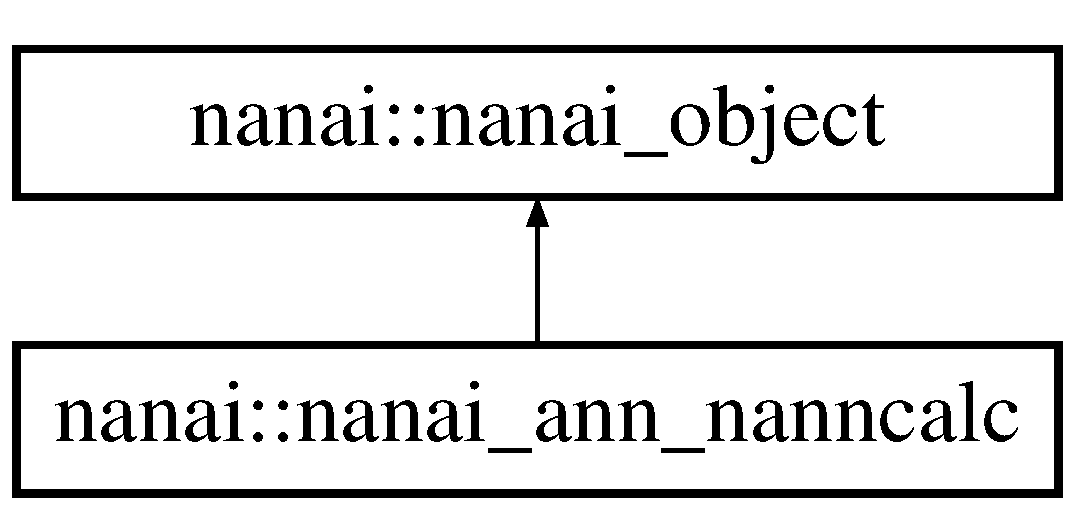
\includegraphics[height=2.000000cm]{classnanai_1_1nanai__ann__nanncalc}
\end{center}
\end{figure}
\subsection*{类}
\begin{DoxyCompactItemize}
\item 
class \hyperlink{classnanai_1_1nanai__ann__nanncalc_1_1ann__t}{ann\+\_\+t}
\item 
struct \hyperlink{structnanai_1_1nanai__ann__nanncalc_1_1ncommand}{ncommand}
\end{DoxyCompactItemize}
\subsection*{Public 成员函数}
\begin{DoxyCompactItemize}
\item 
\hyperlink{classnanai_1_1nanai__ann__nanncalc_a0d26e7efdef5368c0212b3dd02f63767}{nanai\+\_\+ann\+\_\+nanncalc} (\hyperlink{namespacenanai_a892a8c80381d0005a076b68fbbf2d918}{nanai\+\_\+ann\+\_\+nanndesc} \&desc, const char $\ast$lp=\char`\"{}./\char`\"{})
\item 
virtual \hyperlink{classnanai_1_1nanai__ann__nanncalc_a2f5530f782f2585958c79c94bc3232d7}{$\sim$nanai\+\_\+ann\+\_\+nanncalc} ()
\item 
virtual void \hyperlink{classnanai_1_1nanai__ann__nanncalc_a9a2bdcebe0c659e6f6e3466674cc9143}{ann\+\_\+default\+\_\+create} (int ninput, int nhidden, int output, std\+::vector$<$ int $>$ \&nneure)
\item 
virtual void \hyperlink{classnanai_1_1nanai__ann__nanncalc_a0f2a230581dd2c530f35d22d1cd11982}{ann\+\_\+training} (\hyperlink{classnanmath_1_1nanmath__vector}{nanmath\+::nanmath\+\_\+vector} \&input, \hyperlink{classnanmath_1_1nanmath__vector}{nanmath\+::nanmath\+\_\+vector} \&target, const char $\ast$task=N\+U\+L\+L)
\item 
virtual void \hyperlink{classnanai_1_1nanai__ann__nanncalc_a95e5d9672cf1a74e4180389fbf41b899}{ann\+\_\+training\+\_\+notarget} (\hyperlink{classnanmath_1_1nanmath__vector}{nanmath\+::nanmath\+\_\+vector} \&input, const char $\ast$task=N\+U\+L\+L)
\item 
virtual void \hyperlink{classnanai_1_1nanai__ann__nanncalc_a2b1396b5691391e33859c17ab748a39d}{ann\+\_\+training\+\_\+nooutput} (\hyperlink{classnanmath_1_1nanmath__vector}{nanmath\+::nanmath\+\_\+vector} \&input, \hyperlink{classnanmath_1_1nanmath__vector}{nanmath\+::nanmath\+\_\+vector} \&target, const char $\ast$task=N\+U\+L\+L)
\item 
virtual void \hyperlink{classnanai_1_1nanai__ann__nanncalc_a8563aaf57e70ab959dcdec8961af9447}{ann\+\_\+configure} (\hyperlink{namespacenanai_a892a8c80381d0005a076b68fbbf2d918}{nanai\+\_\+ann\+\_\+nanndesc} \&desc)
\item 
virtual void \hyperlink{classnanai_1_1nanai__ann__nanncalc_a6ec3d7893411dcab2edf4e19ae3bb017}{ann\+\_\+exchange} (const \hyperlink{classnanai_1_1nanai__ann__nanncalc_1_1ann__t}{nanai\+\_\+ann\+\_\+nanncalc\+::ann\+\_\+t} \&ann)
\item 
virtual void \hyperlink{classnanai_1_1nanai__ann__nanncalc_ab7c70e33ab6d4ddcc46fcbdd69a14281}{ann\+\_\+stop} ()
\item 
virtual void \hyperlink{classnanai_1_1nanai__ann__nanncalc_a4fb9643a590238c96e8e387022626bd6}{ann\+\_\+destroy} ()
\item 
virtual void \hyperlink{classnanai_1_1nanai__ann__nanncalc_a7b69abc3ab21a6249f360f2c8f319501}{ann\+\_\+wait} (int st=\hyperlink{nanai__ann__nanncalc_8h_abf1ad245b3da2bb8ed628a379ea2c939}{N\+A\+N\+N\+C\+A\+L\+C\+\_\+\+S\+T\+\_\+\+S\+T\+O\+P}, int slt=100)
\item 
virtual \hyperlink{classnanai_1_1nanai__ann__nanncalc_1_1ann__t}{nanai\+\_\+ann\+\_\+nanncalc\+::ann\+\_\+t} \hyperlink{classnanai_1_1nanai__ann__nanncalc_a41ca7081ea2c4244c7013b8edc86e6ba}{ann\+\_\+get} ()
\item 
std\+::string \hyperlink{classnanai_1_1nanai__ann__nanncalc_aa75fcea728a087178b4699a2e2e86a6f}{get\+\_\+task\+\_\+name} () const 
\item 
std\+::string \hyperlink{classnanai_1_1nanai__ann__nanncalc_a19cc8a310068a44c568ada1c9e72d028}{get\+\_\+alg\+\_\+name} () const 
\item 
size\+\_\+t \hyperlink{classnanai_1_1nanai__ann__nanncalc_aa3adf3454d9953ae48e3b0f98ea0cee0}{get\+\_\+cmdlist\+\_\+count} () const 
\item 
virtual void \hyperlink{classnanai_1_1nanai__ann__nanncalc_a0db0e8b62dbea77377e40a5d39f6265c}{set\+\_\+cmd} (struct \hyperlink{structnanai_1_1nanai__ann__nanncalc_1_1ncommand}{ncommand} \&ncmd, bool lock=false)
\item 
virtual int \hyperlink{classnanai_1_1nanai__ann__nanncalc_a18869c97f279df6aa8d467c32fdc7944}{get\+\_\+cmd} (struct \hyperlink{structnanai_1_1nanai__ann__nanncalc_1_1ncommand}{ncommand} \&ncmd, bool lock=false)
\item 
virtual void \hyperlink{classnanai_1_1nanai__ann__nanncalc_a2c8aa9f4f29bb093f0bc26fa9ba6cc41}{set\+\_\+state} (int st, bool lock=false)
\item 
virtual int \hyperlink{classnanai_1_1nanai__ann__nanncalc_abc792abf872514a95a9863cbb3e49cd4}{get\+\_\+state} (bool lock=false)
\item 
virtual void \hyperlink{classnanai_1_1nanai__ann__nanncalc_a5102b94199ba413bd8601e66be5d2293}{set\+\_\+output} (\hyperlink{classnanmath_1_1nanmath__vector}{nanmath\+::nanmath\+\_\+vector} \&output, bool lock=false)
\item 
virtual size\+\_\+t \hyperlink{classnanai_1_1nanai__ann__nanncalc_adc64a3c1efeef53374803673ee44c152}{get\+\_\+output} (\hyperlink{classnanmath_1_1nanmath__vector}{nanmath\+::nanmath\+\_\+vector} \&output, bool lock=false)
\item 
virtual void \hyperlink{classnanai_1_1nanai__ann__nanncalc_ad76affc9e9819af44025704d424ce3ec}{do\+\_\+configure} (\hyperlink{namespacenanai_a892a8c80381d0005a076b68fbbf2d918}{nanai\+\_\+ann\+\_\+nanndesc} \&desc)
\item 
virtual void \hyperlink{classnanai_1_1nanai__ann__nanncalc_a3501b12051f6bb169b408a3671196f16}{do\+\_\+ann\+\_\+exchange} (const \hyperlink{classnanai_1_1nanai__ann__nanncalc_1_1ann__t}{nanai\+\_\+ann\+\_\+nanncalc\+::ann\+\_\+t} \&ann)
\item 
virtual \hyperlink{classnanai_1_1nanai__ann__nanncalc_1_1ann__t}{nanai\+\_\+ann\+\_\+nanncalc\+::ann\+\_\+t} \hyperlink{classnanai_1_1nanai__ann__nanncalc_aefda6586e9dd96625b2e2948baec8e18}{get\+\_\+ann} (bool lock=false)
\item 
virtual void \hyperlink{classnanai_1_1nanai__ann__nanncalc_a1973ea663b28bcc31a7297d75bae139e}{do\+\_\+stop} ()
\item 
virtual void \hyperlink{classnanai_1_1nanai__ann__nanncalc_aeebc06b5241f6f9e1e5b78daa7e31911}{ann\+\_\+calculate} (const char $\ast$task, \hyperlink{classnanmath_1_1nanmath__vector}{nanmath\+::nanmath\+\_\+vector} \&input, \hyperlink{classnanmath_1_1nanmath__vector}{nanmath\+::nanmath\+\_\+vector} $\ast$target, \hyperlink{classnanmath_1_1nanmath__vector}{nanmath\+::nanmath\+\_\+vector} $\ast$output)
\end{DoxyCompactItemize}
\subsection*{Protected 成员函数}
\begin{DoxyCompactItemize}
\item 
virtual void \hyperlink{classnanai_1_1nanai__ann__nanncalc_a59b33730cd75893be549ba6cbe1cd7aa}{ann\+\_\+forward} (\hyperlink{classnanmath_1_1nanmath__vector}{nanmath\+::nanmath\+\_\+vector} \&input, \hyperlink{classnanmath_1_1nanmath__vector}{nanmath\+::nanmath\+\_\+vector} \&output)
\item 
virtual void \hyperlink{classnanai_1_1nanai__ann__nanncalc_af70fe54abb55d464459e2ce4548b1ff2}{ann\+\_\+layer\+\_\+forward} (int h, \hyperlink{classnanmath_1_1nanmath__vector}{nanmath\+::nanmath\+\_\+vector} \&l1, \hyperlink{classnanmath_1_1nanmath__vector}{nanmath\+::nanmath\+\_\+vector} \&l2, \hyperlink{classnanmath_1_1nanmath__matrix}{nanmath\+::nanmath\+\_\+matrix} \&wm, \hyperlink{namespacenanai_a299d9093f72831a48d205e94e200690c}{fptr\+\_\+ann\+\_\+hidden\+\_\+calc} calc)
\item 
virtual \hyperlink{classnanmath_1_1nanmath__vector}{nanmath\+::nanmath\+\_\+vector} \hyperlink{classnanai_1_1nanai__ann__nanncalc_a95e7765ed618d5ab2e4f90593f053d89}{ann\+\_\+output\+\_\+error} (\hyperlink{classnanmath_1_1nanmath__vector}{nanmath\+::nanmath\+\_\+vector} \&target, \hyperlink{classnanmath_1_1nanmath__vector}{nanmath\+::nanmath\+\_\+vector} \&output)
\item 
virtual void \hyperlink{classnanai_1_1nanai__ann__nanncalc_a655e79fd2845915c691081094b02e121}{ann\+\_\+hiddens\+\_\+error} (\hyperlink{classnanmath_1_1nanmath__vector}{nanmath\+::nanmath\+\_\+vector} \&input, \hyperlink{classnanmath_1_1nanmath__vector}{nanmath\+::nanmath\+\_\+vector} \&output\+\_\+delta)
\item 
virtual \hyperlink{classnanmath_1_1nanmath__vector}{nanmath\+::nanmath\+\_\+vector} \hyperlink{classnanai_1_1nanai__ann__nanncalc_ac3254f506152da643ce0dd7b3077ff92}{ann\+\_\+calc\+\_\+hidden\+\_\+delta} (size\+\_\+t h, \hyperlink{classnanmath_1_1nanmath__vector}{nanmath\+::nanmath\+\_\+vector} \&delta\+\_\+k, \hyperlink{classnanmath_1_1nanmath__matrix}{nanmath\+::nanmath\+\_\+matrix} \&w\+\_\+kh, \hyperlink{classnanmath_1_1nanmath__vector}{nanmath\+::nanmath\+\_\+vector} \&o\+\_\+h)
\item 
virtual void \hyperlink{classnanai_1_1nanai__ann__nanncalc_a6066093c9c477445b6bc93261608c1b1}{ann\+\_\+adjust\+\_\+weight} (size\+\_\+t h, \hyperlink{classnanmath_1_1nanmath__vector}{nanmath\+::nanmath\+\_\+vector} \&layer, \hyperlink{classnanmath_1_1nanmath__vector}{nanmath\+::nanmath\+\_\+vector} \&delta)
\item 
virtual void \hyperlink{classnanai_1_1nanai__ann__nanncalc_a675afb775a34013e6aff1f8d669e7de0}{on\+\_\+error} (int err)
\item 
virtual void \hyperlink{classnanai_1_1nanai__ann__nanncalc_a05aa50ca275dade2e3ef735df4a5114d}{ann\+\_\+create} (\hyperlink{namespacenanai_a892a8c80381d0005a076b68fbbf2d918}{nanai\+\_\+ann\+\_\+nanndesc} \&desc)
\item 
virtual void \hyperlink{classnanai_1_1nanai__ann__nanncalc_aa83cff70c2111905341f6b62c9ebd727}{ann\+\_\+on\+\_\+except} (int err)
\item 
virtual void \hyperlink{classnanai_1_1nanai__ann__nanncalc_aa06770b84f20aee6463d57d50c85eb0b}{ann\+\_\+on\+\_\+trained} ()
\item 
virtual void \hyperlink{classnanai_1_1nanai__ann__nanncalc_a718b94361144b9d57eca8e9f665e713a}{ann\+\_\+on\+\_\+trained\+\_\+nooutput} ()
\item 
virtual void \hyperlink{classnanai_1_1nanai__ann__nanncalc_a1d59205c70a0aae1acd02ccd513c64ae}{ann\+\_\+on\+\_\+calculated} ()
\item 
virtual void \hyperlink{classnanai_1_1nanai__ann__nanncalc_ae7fd1a715938713b89830f78bb946c97}{ann\+\_\+on\+\_\+alg\+\_\+uninstall} ()
\item 
virtual void \hyperlink{classnanai_1_1nanai__ann__nanncalc_a20f343f658f4babef5552133159f6c63}{ann\+\_\+process} (int process, void $\ast$arg)
\item 
virtual void \hyperlink{classnanai_1_1nanai__ann__nanncalc_a54ed62943cc681da143bb6a2e1782430}{ann\+\_\+log} (const char $\ast$fmt,...)
\end{DoxyCompactItemize}
\subsection*{Protected 属性}
\begin{DoxyCompactItemize}
\item 
std\+::string \hyperlink{classnanai_1_1nanai__ann__nanncalc_a66ab62c75be9da3951abd85e1eb296e0}{\+\_\+alg}
\item 
std\+::string \hyperlink{classnanai_1_1nanai__ann__nanncalc_ab659b8655ab02f5922ecb19c6418f02c}{\+\_\+task}
\item 
std\+::vector$<$ \hyperlink{classnanmath_1_1nanmath__vector}{nanmath\+::nanmath\+\_\+vector} $>$ \hyperlink{classnanai_1_1nanai__ann__nanncalc_a1e15116b2a2d7b5c8ddb9579de11f5ae}{\+\_\+hiddens}
\item 
pthread\+\_\+mutex\+\_\+t \hyperlink{classnanai_1_1nanai__ann__nanncalc_a1c9006356f22904fee12c3635cdc8a15}{\+\_\+outputs\+\_\+lock}
\item 
std\+::vector$<$ \hyperlink{classnanmath_1_1nanmath__vector}{nanmath\+::nanmath\+\_\+vector} $>$ \hyperlink{classnanai_1_1nanai__ann__nanncalc_a6d00ff0323ee2fd5c1cfbd0f775da125}{\+\_\+outputs}
\item 
\hyperlink{classnanmath_1_1nanmath__vector}{nanmath\+::nanmath\+\_\+vector} \hyperlink{classnanai_1_1nanai__ann__nanncalc_abee00d840fe641d5c69aa1c621333179}{\+\_\+output\+\_\+error}
\item 
pthread\+\_\+mutex\+\_\+t \hyperlink{classnanai_1_1nanai__ann__nanncalc_ab05880760848bb308d30833b362f60a8}{\+\_\+ann\+\_\+lock}
\item 
\hyperlink{classnanai_1_1nanai__ann__nanncalc_1_1ann__t}{ann\+\_\+t} \hyperlink{classnanai_1_1nanai__ann__nanncalc_a3b0bfac7c99ef9d83769efd2936e4638}{\+\_\+ann}
\item 
std\+::queue$<$ struct \hyperlink{structnanai_1_1nanai__ann__nanncalc_1_1ncommand}{ncommand} $>$ \hyperlink{classnanai_1_1nanai__ann__nanncalc_a9af0b8bc21e0d398f3f9489acf1dfab7}{\+\_\+cmdlist}
\item 
pthread\+\_\+mutex\+\_\+t \hyperlink{classnanai_1_1nanai__ann__nanncalc_a92213def4dd3f7f0693159a79446ea09}{\+\_\+cmdlist\+\_\+lock}
\item 
pthread\+\_\+t \hyperlink{classnanai_1_1nanai__ann__nanncalc_ad8115ff56ea159a5e1d43c9752ed5936}{\+\_\+thread\+\_\+worker}
\item 
pthread\+\_\+mutex\+\_\+t \hyperlink{classnanai_1_1nanai__ann__nanncalc_a25ab2c0cf73a5ff7201ad1cd339626dc}{\+\_\+state\+\_\+lock}
\item 
int \hyperlink{classnanai_1_1nanai__ann__nanncalc_a1b2991833f76b5400e371f01ad7c6bbc}{\+\_\+state}
\item 
int \hyperlink{classnanai_1_1nanai__ann__nanncalc_a9834cef878366ef0bab79c5538a9f3be}{\+\_\+command}
\item 
int \hyperlink{classnanai_1_1nanai__ann__nanncalc_ad5c0182fd45d65dd7d91439d4eec6119}{\+\_\+sleep\+\_\+time}
\item 
\hyperlink{namespacenanai_a681d28f80aa95597ffc268b3b01abcfc}{fptr\+\_\+ann\+\_\+input\+\_\+filter} \hyperlink{classnanai_1_1nanai__ann__nanncalc_abebe28725dd1424ef5cd915f0146f56c}{\+\_\+fptr\+\_\+input\+\_\+filter}
\item 
\hyperlink{namespacenanai_ab737ac3c4f32f96a8ee6400db1c5a90f}{fptr\+\_\+ann\+\_\+result} \hyperlink{classnanai_1_1nanai__ann__nanncalc_afdaafe5d48d6590d9c38b020452eabce}{\+\_\+fptr\+\_\+result}
\item 
\hyperlink{namespacenanai_a5e697a4846a90e7e161e1d2d5be57688}{fptr\+\_\+ann\+\_\+output\+\_\+error} \hyperlink{classnanai_1_1nanai__ann__nanncalc_ac3d0e7fa0ac6210163391e0971f306cb}{\+\_\+fptr\+\_\+output\+\_\+error}
\item 
\hyperlink{namespacenanai_ac1a3ebd721fc3cfe1b9accfe7b65b7fe}{fptr\+\_\+ann\+\_\+calculate} \hyperlink{classnanai_1_1nanai__ann__nanncalc_afc0f3e68d5bc6d690d77f7ec938b2586}{\+\_\+fptr\+\_\+calculate}
\item 
\hyperlink{namespacenanai_a5fc4ff646e59919360af1ef410fe9671}{fptr\+\_\+ann\+\_\+hidden\+\_\+init} \hyperlink{classnanai_1_1nanai__ann__nanncalc_a8c430665e02d65d174eac790bb163341}{\+\_\+fptr\+\_\+hidden\+\_\+inits}
\item 
\hyperlink{namespacenanai_a299d9093f72831a48d205e94e200690c}{fptr\+\_\+ann\+\_\+hidden\+\_\+calc} \hyperlink{classnanai_1_1nanai__ann__nanncalc_a37c34eacc9c875653b79b4636596d4d3}{\+\_\+fptr\+\_\+hidden\+\_\+calcs}
\item 
\hyperlink{namespacenanai_aa8cd8d38cbd0a27e2818f132a3cfa2a2}{fptr\+\_\+ann\+\_\+hidden\+\_\+error} \hyperlink{classnanai_1_1nanai__ann__nanncalc_a6b4c7a5a93bd5d46f4ef78f5256963c7}{\+\_\+fptr\+\_\+hidden\+\_\+errors}
\item 
\hyperlink{namespacenanai_a1d9a4524c199b1a2891e208ce4b05306}{fptr\+\_\+ann\+\_\+hidden\+\_\+adjust\+\_\+weight} \hyperlink{classnanai_1_1nanai__ann__nanncalc_a90ca7f0507edefeb6c2b14641bbee7e9}{\+\_\+fptr\+\_\+hidden\+\_\+adjust\+\_\+weights}
\item 
\hyperlink{namespacenanai_ad9527fac6e647a6c149e4f9a8681e4c1}{fptr\+\_\+ann\+\_\+monitor\+\_\+except} \hyperlink{classnanai_1_1nanai__ann__nanncalc_a34ae5583c27674e94782b1491732139c}{\+\_\+callback\+\_\+monitor\+\_\+except}
\item 
\hyperlink{namespacenanai_adb209ab120b98e800db2b0c8621cd488}{fptr\+\_\+ann\+\_\+monitor\+\_\+trained} \hyperlink{classnanai_1_1nanai__ann__nanncalc_abe6bd5a48bafb89a185a8e359ffdcff3}{\+\_\+callback\+\_\+monitor\+\_\+trained}
\item 
\hyperlink{namespacenanai_a598e872bf861dac8080e98d6d155b3b5}{fptr\+\_\+ann\+\_\+monitor\+\_\+trained2} \hyperlink{classnanai_1_1nanai__ann__nanncalc_a0395dff2948785f646f22be1df04bad1}{\+\_\+callback\+\_\+monitor\+\_\+trained\+\_\+nooutput}
\item 
\hyperlink{namespacenanai_afc00080af95a1dc2349880f03d7d6a88}{fptr\+\_\+ann\+\_\+monitor\+\_\+calculated} \hyperlink{classnanai_1_1nanai__ann__nanncalc_af9ee346f2307a03b8570ec21839a3e88}{\+\_\+callback\+\_\+monitor\+\_\+calculated}
\item 
\hyperlink{namespacenanai_a5c9964edbd4db8ae35df7cd024020e87}{fptr\+\_\+ann\+\_\+monitor\+\_\+progress} \hyperlink{classnanai_1_1nanai__ann__nanncalc_af937dc713e3780b86b5ebf2311360dd7}{\+\_\+callback\+\_\+monitor\+\_\+progress}
\item 
\hyperlink{namespacenanai_a04b231ce428a771ab1a9aace53be65c6}{fptr\+\_\+ann\+\_\+monitor\+\_\+alg\+\_\+uninstall} \hyperlink{classnanai_1_1nanai__ann__nanncalc_a524fbed26f582cdf403407173da1634b}{\+\_\+callback\+\_\+monitor\+\_\+alg\+\_\+uninstall}
\item 
F\+I\+L\+E $\ast$ \hyperlink{classnanai_1_1nanai__ann__nanncalc_ad7f1e9a64ffdf10347e0f7175a73103c}{\+\_\+log\+\_\+file}
\item 
std\+::string \hyperlink{classnanai_1_1nanai__ann__nanncalc_ad02491864e160b837d6b84f635f5947a}{\+\_\+log\+\_\+dir}
\end{DoxyCompactItemize}


\subsection{详细描述}


在文件 nanai\+\_\+ann\+\_\+nanncalc.\+h 第 46 行定义.



\subsection{构造及析构函数说明}
\hypertarget{classnanai_1_1nanai__ann__nanncalc_a0d26e7efdef5368c0212b3dd02f63767}{}\index{nanai\+::nanai\+\_\+ann\+\_\+nanncalc@{nanai\+::nanai\+\_\+ann\+\_\+nanncalc}!nanai\+\_\+ann\+\_\+nanncalc@{nanai\+\_\+ann\+\_\+nanncalc}}
\index{nanai\+\_\+ann\+\_\+nanncalc@{nanai\+\_\+ann\+\_\+nanncalc}!nanai\+::nanai\+\_\+ann\+\_\+nanncalc@{nanai\+::nanai\+\_\+ann\+\_\+nanncalc}}
\subsubsection[{nanai\+\_\+ann\+\_\+nanncalc(nanai\+\_\+ann\+\_\+nanndesc \&desc, const char $\ast$lp=""./"")}]{\setlength{\rightskip}{0pt plus 5cm}nanai\+::nanai\+\_\+ann\+\_\+nanncalc\+::nanai\+\_\+ann\+\_\+nanncalc (
\begin{DoxyParamCaption}
\item[{{\bf nanai\+\_\+ann\+\_\+nanndesc} \&}]{desc, }
\item[{const char $\ast$}]{lp = {\ttfamily \char`\"{}./\char`\"{}}}
\end{DoxyParamCaption}
)}\label{classnanai_1_1nanai__ann__nanncalc_a0d26e7efdef5368c0212b3dd02f63767}


在文件 nanai\+\_\+ann\+\_\+nanncalc.\+cc 第 153 行定义.

\hypertarget{classnanai_1_1nanai__ann__nanncalc_a2f5530f782f2585958c79c94bc3232d7}{}\index{nanai\+::nanai\+\_\+ann\+\_\+nanncalc@{nanai\+::nanai\+\_\+ann\+\_\+nanncalc}!````~nanai\+\_\+ann\+\_\+nanncalc@{$\sim$nanai\+\_\+ann\+\_\+nanncalc}}
\index{````~nanai\+\_\+ann\+\_\+nanncalc@{$\sim$nanai\+\_\+ann\+\_\+nanncalc}!nanai\+::nanai\+\_\+ann\+\_\+nanncalc@{nanai\+::nanai\+\_\+ann\+\_\+nanncalc}}
\subsubsection[{$\sim$nanai\+\_\+ann\+\_\+nanncalc()}]{\setlength{\rightskip}{0pt plus 5cm}nanai\+::nanai\+\_\+ann\+\_\+nanncalc\+::$\sim$nanai\+\_\+ann\+\_\+nanncalc (
\begin{DoxyParamCaption}
{}
\end{DoxyParamCaption}
)\hspace{0.3cm}{\ttfamily [virtual]}}\label{classnanai_1_1nanai__ann__nanncalc_a2f5530f782f2585958c79c94bc3232d7}


在文件 nanai\+\_\+ann\+\_\+nanncalc.\+cc 第 222 行定义.



\subsection{成员函数说明}
\hypertarget{classnanai_1_1nanai__ann__nanncalc_a6066093c9c477445b6bc93261608c1b1}{}\index{nanai\+::nanai\+\_\+ann\+\_\+nanncalc@{nanai\+::nanai\+\_\+ann\+\_\+nanncalc}!ann\+\_\+adjust\+\_\+weight@{ann\+\_\+adjust\+\_\+weight}}
\index{ann\+\_\+adjust\+\_\+weight@{ann\+\_\+adjust\+\_\+weight}!nanai\+::nanai\+\_\+ann\+\_\+nanncalc@{nanai\+::nanai\+\_\+ann\+\_\+nanncalc}}
\subsubsection[{ann\+\_\+adjust\+\_\+weight(size\+\_\+t h, nanmath\+::nanmath\+\_\+vector \&layer, nanmath\+::nanmath\+\_\+vector \&delta)}]{\setlength{\rightskip}{0pt plus 5cm}void nanai\+::nanai\+\_\+ann\+\_\+nanncalc\+::ann\+\_\+adjust\+\_\+weight (
\begin{DoxyParamCaption}
\item[{size\+\_\+t}]{h, }
\item[{{\bf nanmath\+::nanmath\+\_\+vector} \&}]{layer, }
\item[{{\bf nanmath\+::nanmath\+\_\+vector} \&}]{delta}
\end{DoxyParamCaption}
)\hspace{0.3cm}{\ttfamily [protected]}, {\ttfamily [virtual]}}\label{classnanai_1_1nanai__ann__nanncalc_a6066093c9c477445b6bc93261608c1b1}


在文件 nanai\+\_\+ann\+\_\+nanncalc.\+cc 第 885 行定义.

\hypertarget{classnanai_1_1nanai__ann__nanncalc_ac3254f506152da643ce0dd7b3077ff92}{}\index{nanai\+::nanai\+\_\+ann\+\_\+nanncalc@{nanai\+::nanai\+\_\+ann\+\_\+nanncalc}!ann\+\_\+calc\+\_\+hidden\+\_\+delta@{ann\+\_\+calc\+\_\+hidden\+\_\+delta}}
\index{ann\+\_\+calc\+\_\+hidden\+\_\+delta@{ann\+\_\+calc\+\_\+hidden\+\_\+delta}!nanai\+::nanai\+\_\+ann\+\_\+nanncalc@{nanai\+::nanai\+\_\+ann\+\_\+nanncalc}}
\subsubsection[{ann\+\_\+calc\+\_\+hidden\+\_\+delta(size\+\_\+t h, nanmath\+::nanmath\+\_\+vector \&delta\+\_\+k, nanmath\+::nanmath\+\_\+matrix \&w\+\_\+kh, nanmath\+::nanmath\+\_\+vector \&o\+\_\+h)}]{\setlength{\rightskip}{0pt plus 5cm}{\bf nanmath\+::nanmath\+\_\+vector} nanai\+::nanai\+\_\+ann\+\_\+nanncalc\+::ann\+\_\+calc\+\_\+hidden\+\_\+delta (
\begin{DoxyParamCaption}
\item[{size\+\_\+t}]{h, }
\item[{{\bf nanmath\+::nanmath\+\_\+vector} \&}]{delta\+\_\+k, }
\item[{{\bf nanmath\+::nanmath\+\_\+matrix} \&}]{w\+\_\+kh, }
\item[{{\bf nanmath\+::nanmath\+\_\+vector} \&}]{o\+\_\+h}
\end{DoxyParamCaption}
)\hspace{0.3cm}{\ttfamily [protected]}, {\ttfamily [virtual]}}\label{classnanai_1_1nanai__ann__nanncalc_ac3254f506152da643ce0dd7b3077ff92}


在文件 nanai\+\_\+ann\+\_\+nanncalc.\+cc 第 832 行定义.

\hypertarget{classnanai_1_1nanai__ann__nanncalc_aeebc06b5241f6f9e1e5b78daa7e31911}{}\index{nanai\+::nanai\+\_\+ann\+\_\+nanncalc@{nanai\+::nanai\+\_\+ann\+\_\+nanncalc}!ann\+\_\+calculate@{ann\+\_\+calculate}}
\index{ann\+\_\+calculate@{ann\+\_\+calculate}!nanai\+::nanai\+\_\+ann\+\_\+nanncalc@{nanai\+::nanai\+\_\+ann\+\_\+nanncalc}}
\subsubsection[{ann\+\_\+calculate(const char $\ast$task, nanmath\+::nanmath\+\_\+vector \&input, nanmath\+::nanmath\+\_\+vector $\ast$target, nanmath\+::nanmath\+\_\+vector $\ast$output)}]{\setlength{\rightskip}{0pt plus 5cm}void nanai\+::nanai\+\_\+ann\+\_\+nanncalc\+::ann\+\_\+calculate (
\begin{DoxyParamCaption}
\item[{const char $\ast$}]{task, }
\item[{{\bf nanmath\+::nanmath\+\_\+vector} \&}]{input, }
\item[{{\bf nanmath\+::nanmath\+\_\+vector} $\ast$}]{target, }
\item[{{\bf nanmath\+::nanmath\+\_\+vector} $\ast$}]{output}
\end{DoxyParamCaption}
)\hspace{0.3cm}{\ttfamily [virtual]}}\label{classnanai_1_1nanai__ann__nanncalc_aeebc06b5241f6f9e1e5b78daa7e31911}


在文件 nanai\+\_\+ann\+\_\+nanncalc.\+cc 第 703 行定义.

\hypertarget{classnanai_1_1nanai__ann__nanncalc_a8563aaf57e70ab959dcdec8961af9447}{}\index{nanai\+::nanai\+\_\+ann\+\_\+nanncalc@{nanai\+::nanai\+\_\+ann\+\_\+nanncalc}!ann\+\_\+configure@{ann\+\_\+configure}}
\index{ann\+\_\+configure@{ann\+\_\+configure}!nanai\+::nanai\+\_\+ann\+\_\+nanncalc@{nanai\+::nanai\+\_\+ann\+\_\+nanncalc}}
\subsubsection[{ann\+\_\+configure(nanai\+\_\+ann\+\_\+nanndesc \&desc)}]{\setlength{\rightskip}{0pt plus 5cm}void nanai\+::nanai\+\_\+ann\+\_\+nanncalc\+::ann\+\_\+configure (
\begin{DoxyParamCaption}
\item[{{\bf nanai\+\_\+ann\+\_\+nanndesc} \&}]{desc}
\end{DoxyParamCaption}
)\hspace{0.3cm}{\ttfamily [virtual]}}\label{classnanai_1_1nanai__ann__nanncalc_a8563aaf57e70ab959dcdec8961af9447}


在文件 nanai\+\_\+ann\+\_\+nanncalc.\+cc 第 303 行定义.

\hypertarget{classnanai_1_1nanai__ann__nanncalc_a05aa50ca275dade2e3ef735df4a5114d}{}\index{nanai\+::nanai\+\_\+ann\+\_\+nanncalc@{nanai\+::nanai\+\_\+ann\+\_\+nanncalc}!ann\+\_\+create@{ann\+\_\+create}}
\index{ann\+\_\+create@{ann\+\_\+create}!nanai\+::nanai\+\_\+ann\+\_\+nanncalc@{nanai\+::nanai\+\_\+ann\+\_\+nanncalc}}
\subsubsection[{ann\+\_\+create(nanai\+\_\+ann\+\_\+nanndesc \&desc)}]{\setlength{\rightskip}{0pt plus 5cm}void nanai\+::nanai\+\_\+ann\+\_\+nanncalc\+::ann\+\_\+create (
\begin{DoxyParamCaption}
\item[{{\bf nanai\+\_\+ann\+\_\+nanndesc} \&}]{desc}
\end{DoxyParamCaption}
)\hspace{0.3cm}{\ttfamily [protected]}, {\ttfamily [virtual]}}\label{classnanai_1_1nanai__ann__nanncalc_a05aa50ca275dade2e3ef735df4a5114d}


在文件 nanai\+\_\+ann\+\_\+nanncalc.\+cc 第 560 行定义.

\hypertarget{classnanai_1_1nanai__ann__nanncalc_a9a2bdcebe0c659e6f6e3466674cc9143}{}\index{nanai\+::nanai\+\_\+ann\+\_\+nanncalc@{nanai\+::nanai\+\_\+ann\+\_\+nanncalc}!ann\+\_\+default\+\_\+create@{ann\+\_\+default\+\_\+create}}
\index{ann\+\_\+default\+\_\+create@{ann\+\_\+default\+\_\+create}!nanai\+::nanai\+\_\+ann\+\_\+nanncalc@{nanai\+::nanai\+\_\+ann\+\_\+nanncalc}}
\subsubsection[{ann\+\_\+default\+\_\+create(int ninput, int nhidden, int output, std\+::vector$<$ int $>$ \&nneure)}]{\setlength{\rightskip}{0pt plus 5cm}void nanai\+::nanai\+\_\+ann\+\_\+nanncalc\+::ann\+\_\+default\+\_\+create (
\begin{DoxyParamCaption}
\item[{int}]{ninput, }
\item[{int}]{nhidden, }
\item[{int}]{output, }
\item[{std\+::vector$<$ int $>$ \&}]{nneure}
\end{DoxyParamCaption}
)\hspace{0.3cm}{\ttfamily [virtual]}}\label{classnanai_1_1nanai__ann__nanncalc_a9a2bdcebe0c659e6f6e3466674cc9143}


在文件 nanai\+\_\+ann\+\_\+nanncalc.\+cc 第 252 行定义.

\hypertarget{classnanai_1_1nanai__ann__nanncalc_a4fb9643a590238c96e8e387022626bd6}{}\index{nanai\+::nanai\+\_\+ann\+\_\+nanncalc@{nanai\+::nanai\+\_\+ann\+\_\+nanncalc}!ann\+\_\+destroy@{ann\+\_\+destroy}}
\index{ann\+\_\+destroy@{ann\+\_\+destroy}!nanai\+::nanai\+\_\+ann\+\_\+nanncalc@{nanai\+::nanai\+\_\+ann\+\_\+nanncalc}}
\subsubsection[{ann\+\_\+destroy()}]{\setlength{\rightskip}{0pt plus 5cm}void nanai\+::nanai\+\_\+ann\+\_\+nanncalc\+::ann\+\_\+destroy (
\begin{DoxyParamCaption}
{}
\end{DoxyParamCaption}
)\hspace{0.3cm}{\ttfamily [virtual]}}\label{classnanai_1_1nanai__ann__nanncalc_a4fb9643a590238c96e8e387022626bd6}


在文件 nanai\+\_\+ann\+\_\+nanncalc.\+cc 第 336 行定义.

\hypertarget{classnanai_1_1nanai__ann__nanncalc_a6ec3d7893411dcab2edf4e19ae3bb017}{}\index{nanai\+::nanai\+\_\+ann\+\_\+nanncalc@{nanai\+::nanai\+\_\+ann\+\_\+nanncalc}!ann\+\_\+exchange@{ann\+\_\+exchange}}
\index{ann\+\_\+exchange@{ann\+\_\+exchange}!nanai\+::nanai\+\_\+ann\+\_\+nanncalc@{nanai\+::nanai\+\_\+ann\+\_\+nanncalc}}
\subsubsection[{ann\+\_\+exchange(const nanai\+\_\+ann\+\_\+nanncalc\+::ann\+\_\+t \&ann)}]{\setlength{\rightskip}{0pt plus 5cm}void nanai\+::nanai\+\_\+ann\+\_\+nanncalc\+::ann\+\_\+exchange (
\begin{DoxyParamCaption}
\item[{const {\bf nanai\+\_\+ann\+\_\+nanncalc\+::ann\+\_\+t} \&}]{ann}
\end{DoxyParamCaption}
)\hspace{0.3cm}{\ttfamily [virtual]}}\label{classnanai_1_1nanai__ann__nanncalc_a6ec3d7893411dcab2edf4e19ae3bb017}


在文件 nanai\+\_\+ann\+\_\+nanncalc.\+cc 第 310 行定义.

\hypertarget{classnanai_1_1nanai__ann__nanncalc_a59b33730cd75893be549ba6cbe1cd7aa}{}\index{nanai\+::nanai\+\_\+ann\+\_\+nanncalc@{nanai\+::nanai\+\_\+ann\+\_\+nanncalc}!ann\+\_\+forward@{ann\+\_\+forward}}
\index{ann\+\_\+forward@{ann\+\_\+forward}!nanai\+::nanai\+\_\+ann\+\_\+nanncalc@{nanai\+::nanai\+\_\+ann\+\_\+nanncalc}}
\subsubsection[{ann\+\_\+forward(nanmath\+::nanmath\+\_\+vector \&input, nanmath\+::nanmath\+\_\+vector \&output)}]{\setlength{\rightskip}{0pt plus 5cm}void nanai\+::nanai\+\_\+ann\+\_\+nanncalc\+::ann\+\_\+forward (
\begin{DoxyParamCaption}
\item[{{\bf nanmath\+::nanmath\+\_\+vector} \&}]{input, }
\item[{{\bf nanmath\+::nanmath\+\_\+vector} \&}]{output}
\end{DoxyParamCaption}
)\hspace{0.3cm}{\ttfamily [protected]}, {\ttfamily [virtual]}}\label{classnanai_1_1nanai__ann__nanncalc_a59b33730cd75893be549ba6cbe1cd7aa}


在文件 nanai\+\_\+ann\+\_\+nanncalc.\+cc 第 746 行定义.

\hypertarget{classnanai_1_1nanai__ann__nanncalc_a41ca7081ea2c4244c7013b8edc86e6ba}{}\index{nanai\+::nanai\+\_\+ann\+\_\+nanncalc@{nanai\+::nanai\+\_\+ann\+\_\+nanncalc}!ann\+\_\+get@{ann\+\_\+get}}
\index{ann\+\_\+get@{ann\+\_\+get}!nanai\+::nanai\+\_\+ann\+\_\+nanncalc@{nanai\+::nanai\+\_\+ann\+\_\+nanncalc}}
\subsubsection[{ann\+\_\+get()}]{\setlength{\rightskip}{0pt plus 5cm}{\bf nanai\+\_\+ann\+\_\+nanncalc\+::ann\+\_\+t} nanai\+::nanai\+\_\+ann\+\_\+nanncalc\+::ann\+\_\+get (
\begin{DoxyParamCaption}
{}
\end{DoxyParamCaption}
)\hspace{0.3cm}{\ttfamily [virtual]}}\label{classnanai_1_1nanai__ann__nanncalc_a41ca7081ea2c4244c7013b8edc86e6ba}


在文件 nanai\+\_\+ann\+\_\+nanncalc.\+cc 第 374 行定义.

\hypertarget{classnanai_1_1nanai__ann__nanncalc_a655e79fd2845915c691081094b02e121}{}\index{nanai\+::nanai\+\_\+ann\+\_\+nanncalc@{nanai\+::nanai\+\_\+ann\+\_\+nanncalc}!ann\+\_\+hiddens\+\_\+error@{ann\+\_\+hiddens\+\_\+error}}
\index{ann\+\_\+hiddens\+\_\+error@{ann\+\_\+hiddens\+\_\+error}!nanai\+::nanai\+\_\+ann\+\_\+nanncalc@{nanai\+::nanai\+\_\+ann\+\_\+nanncalc}}
\subsubsection[{ann\+\_\+hiddens\+\_\+error(nanmath\+::nanmath\+\_\+vector \&input, nanmath\+::nanmath\+\_\+vector \&output\+\_\+delta)}]{\setlength{\rightskip}{0pt plus 5cm}void nanai\+::nanai\+\_\+ann\+\_\+nanncalc\+::ann\+\_\+hiddens\+\_\+error (
\begin{DoxyParamCaption}
\item[{{\bf nanmath\+::nanmath\+\_\+vector} \&}]{input, }
\item[{{\bf nanmath\+::nanmath\+\_\+vector} \&}]{output\+\_\+delta}
\end{DoxyParamCaption}
)\hspace{0.3cm}{\ttfamily [protected]}, {\ttfamily [virtual]}}\label{classnanai_1_1nanai__ann__nanncalc_a655e79fd2845915c691081094b02e121}


在文件 nanai\+\_\+ann\+\_\+nanncalc.\+cc 第 846 行定义.

\hypertarget{classnanai_1_1nanai__ann__nanncalc_af70fe54abb55d464459e2ce4548b1ff2}{}\index{nanai\+::nanai\+\_\+ann\+\_\+nanncalc@{nanai\+::nanai\+\_\+ann\+\_\+nanncalc}!ann\+\_\+layer\+\_\+forward@{ann\+\_\+layer\+\_\+forward}}
\index{ann\+\_\+layer\+\_\+forward@{ann\+\_\+layer\+\_\+forward}!nanai\+::nanai\+\_\+ann\+\_\+nanncalc@{nanai\+::nanai\+\_\+ann\+\_\+nanncalc}}
\subsubsection[{ann\+\_\+layer\+\_\+forward(int h, nanmath\+::nanmath\+\_\+vector \&l1, nanmath\+::nanmath\+\_\+vector \&l2, nanmath\+::nanmath\+\_\+matrix \&wm, fptr\+\_\+ann\+\_\+hidden\+\_\+calc calc)}]{\setlength{\rightskip}{0pt plus 5cm}void nanai\+::nanai\+\_\+ann\+\_\+nanncalc\+::ann\+\_\+layer\+\_\+forward (
\begin{DoxyParamCaption}
\item[{int}]{h, }
\item[{{\bf nanmath\+::nanmath\+\_\+vector} \&}]{l1, }
\item[{{\bf nanmath\+::nanmath\+\_\+vector} \&}]{l2, }
\item[{{\bf nanmath\+::nanmath\+\_\+matrix} \&}]{wm, }
\item[{{\bf fptr\+\_\+ann\+\_\+hidden\+\_\+calc}}]{calc}
\end{DoxyParamCaption}
)\hspace{0.3cm}{\ttfamily [protected]}, {\ttfamily [virtual]}}\label{classnanai_1_1nanai__ann__nanncalc_af70fe54abb55d464459e2ce4548b1ff2}


在文件 nanai\+\_\+ann\+\_\+nanncalc.\+cc 第 782 行定义.

\hypertarget{classnanai_1_1nanai__ann__nanncalc_a54ed62943cc681da143bb6a2e1782430}{}\index{nanai\+::nanai\+\_\+ann\+\_\+nanncalc@{nanai\+::nanai\+\_\+ann\+\_\+nanncalc}!ann\+\_\+log@{ann\+\_\+log}}
\index{ann\+\_\+log@{ann\+\_\+log}!nanai\+::nanai\+\_\+ann\+\_\+nanncalc@{nanai\+::nanai\+\_\+ann\+\_\+nanncalc}}
\subsubsection[{ann\+\_\+log(const char $\ast$fmt,...)}]{\setlength{\rightskip}{0pt plus 5cm}void nanai\+::nanai\+\_\+ann\+\_\+nanncalc\+::ann\+\_\+log (
\begin{DoxyParamCaption}
\item[{const char $\ast$}]{fmt, }
\item[{}]{...}
\end{DoxyParamCaption}
)\hspace{0.3cm}{\ttfamily [protected]}, {\ttfamily [virtual]}}\label{classnanai_1_1nanai__ann__nanncalc_a54ed62943cc681da143bb6a2e1782430}


在文件 nanai\+\_\+ann\+\_\+nanncalc.\+cc 第 681 行定义.

\hypertarget{classnanai_1_1nanai__ann__nanncalc_ae7fd1a715938713b89830f78bb946c97}{}\index{nanai\+::nanai\+\_\+ann\+\_\+nanncalc@{nanai\+::nanai\+\_\+ann\+\_\+nanncalc}!ann\+\_\+on\+\_\+alg\+\_\+uninstall@{ann\+\_\+on\+\_\+alg\+\_\+uninstall}}
\index{ann\+\_\+on\+\_\+alg\+\_\+uninstall@{ann\+\_\+on\+\_\+alg\+\_\+uninstall}!nanai\+::nanai\+\_\+ann\+\_\+nanncalc@{nanai\+::nanai\+\_\+ann\+\_\+nanncalc}}
\subsubsection[{ann\+\_\+on\+\_\+alg\+\_\+uninstall()}]{\setlength{\rightskip}{0pt plus 5cm}void nanai\+::nanai\+\_\+ann\+\_\+nanncalc\+::ann\+\_\+on\+\_\+alg\+\_\+uninstall (
\begin{DoxyParamCaption}
{}
\end{DoxyParamCaption}
)\hspace{0.3cm}{\ttfamily [protected]}, {\ttfamily [virtual]}}\label{classnanai_1_1nanai__ann__nanncalc_ae7fd1a715938713b89830f78bb946c97}


在文件 nanai\+\_\+ann\+\_\+nanncalc.\+cc 第 667 行定义.

\hypertarget{classnanai_1_1nanai__ann__nanncalc_a1d59205c70a0aae1acd02ccd513c64ae}{}\index{nanai\+::nanai\+\_\+ann\+\_\+nanncalc@{nanai\+::nanai\+\_\+ann\+\_\+nanncalc}!ann\+\_\+on\+\_\+calculated@{ann\+\_\+on\+\_\+calculated}}
\index{ann\+\_\+on\+\_\+calculated@{ann\+\_\+on\+\_\+calculated}!nanai\+::nanai\+\_\+ann\+\_\+nanncalc@{nanai\+::nanai\+\_\+ann\+\_\+nanncalc}}
\subsubsection[{ann\+\_\+on\+\_\+calculated()}]{\setlength{\rightskip}{0pt plus 5cm}void nanai\+::nanai\+\_\+ann\+\_\+nanncalc\+::ann\+\_\+on\+\_\+calculated (
\begin{DoxyParamCaption}
{}
\end{DoxyParamCaption}
)\hspace{0.3cm}{\ttfamily [protected]}, {\ttfamily [virtual]}}\label{classnanai_1_1nanai__ann__nanncalc_a1d59205c70a0aae1acd02ccd513c64ae}


在文件 nanai\+\_\+ann\+\_\+nanncalc.\+cc 第 659 行定义.

\hypertarget{classnanai_1_1nanai__ann__nanncalc_aa83cff70c2111905341f6b62c9ebd727}{}\index{nanai\+::nanai\+\_\+ann\+\_\+nanncalc@{nanai\+::nanai\+\_\+ann\+\_\+nanncalc}!ann\+\_\+on\+\_\+except@{ann\+\_\+on\+\_\+except}}
\index{ann\+\_\+on\+\_\+except@{ann\+\_\+on\+\_\+except}!nanai\+::nanai\+\_\+ann\+\_\+nanncalc@{nanai\+::nanai\+\_\+ann\+\_\+nanncalc}}
\subsubsection[{ann\+\_\+on\+\_\+except(int err)}]{\setlength{\rightskip}{0pt plus 5cm}void nanai\+::nanai\+\_\+ann\+\_\+nanncalc\+::ann\+\_\+on\+\_\+except (
\begin{DoxyParamCaption}
\item[{int}]{err}
\end{DoxyParamCaption}
)\hspace{0.3cm}{\ttfamily [protected]}, {\ttfamily [virtual]}}\label{classnanai_1_1nanai__ann__nanncalc_aa83cff70c2111905341f6b62c9ebd727}


在文件 nanai\+\_\+ann\+\_\+nanncalc.\+cc 第 634 行定义.

\hypertarget{classnanai_1_1nanai__ann__nanncalc_aa06770b84f20aee6463d57d50c85eb0b}{}\index{nanai\+::nanai\+\_\+ann\+\_\+nanncalc@{nanai\+::nanai\+\_\+ann\+\_\+nanncalc}!ann\+\_\+on\+\_\+trained@{ann\+\_\+on\+\_\+trained}}
\index{ann\+\_\+on\+\_\+trained@{ann\+\_\+on\+\_\+trained}!nanai\+::nanai\+\_\+ann\+\_\+nanncalc@{nanai\+::nanai\+\_\+ann\+\_\+nanncalc}}
\subsubsection[{ann\+\_\+on\+\_\+trained()}]{\setlength{\rightskip}{0pt plus 5cm}void nanai\+::nanai\+\_\+ann\+\_\+nanncalc\+::ann\+\_\+on\+\_\+trained (
\begin{DoxyParamCaption}
{}
\end{DoxyParamCaption}
)\hspace{0.3cm}{\ttfamily [protected]}, {\ttfamily [virtual]}}\label{classnanai_1_1nanai__ann__nanncalc_aa06770b84f20aee6463d57d50c85eb0b}


在文件 nanai\+\_\+ann\+\_\+nanncalc.\+cc 第 643 行定义.

\hypertarget{classnanai_1_1nanai__ann__nanncalc_a718b94361144b9d57eca8e9f665e713a}{}\index{nanai\+::nanai\+\_\+ann\+\_\+nanncalc@{nanai\+::nanai\+\_\+ann\+\_\+nanncalc}!ann\+\_\+on\+\_\+trained\+\_\+nooutput@{ann\+\_\+on\+\_\+trained\+\_\+nooutput}}
\index{ann\+\_\+on\+\_\+trained\+\_\+nooutput@{ann\+\_\+on\+\_\+trained\+\_\+nooutput}!nanai\+::nanai\+\_\+ann\+\_\+nanncalc@{nanai\+::nanai\+\_\+ann\+\_\+nanncalc}}
\subsubsection[{ann\+\_\+on\+\_\+trained\+\_\+nooutput()}]{\setlength{\rightskip}{0pt plus 5cm}void nanai\+::nanai\+\_\+ann\+\_\+nanncalc\+::ann\+\_\+on\+\_\+trained\+\_\+nooutput (
\begin{DoxyParamCaption}
{}
\end{DoxyParamCaption}
)\hspace{0.3cm}{\ttfamily [protected]}, {\ttfamily [virtual]}}\label{classnanai_1_1nanai__ann__nanncalc_a718b94361144b9d57eca8e9f665e713a}


在文件 nanai\+\_\+ann\+\_\+nanncalc.\+cc 第 651 行定义.

\hypertarget{classnanai_1_1nanai__ann__nanncalc_a95e7765ed618d5ab2e4f90593f053d89}{}\index{nanai\+::nanai\+\_\+ann\+\_\+nanncalc@{nanai\+::nanai\+\_\+ann\+\_\+nanncalc}!ann\+\_\+output\+\_\+error@{ann\+\_\+output\+\_\+error}}
\index{ann\+\_\+output\+\_\+error@{ann\+\_\+output\+\_\+error}!nanai\+::nanai\+\_\+ann\+\_\+nanncalc@{nanai\+::nanai\+\_\+ann\+\_\+nanncalc}}
\subsubsection[{ann\+\_\+output\+\_\+error(nanmath\+::nanmath\+\_\+vector \&target, nanmath\+::nanmath\+\_\+vector \&output)}]{\setlength{\rightskip}{0pt plus 5cm}{\bf nanmath\+::nanmath\+\_\+vector} nanai\+::nanai\+\_\+ann\+\_\+nanncalc\+::ann\+\_\+output\+\_\+error (
\begin{DoxyParamCaption}
\item[{{\bf nanmath\+::nanmath\+\_\+vector} \&}]{target, }
\item[{{\bf nanmath\+::nanmath\+\_\+vector} \&}]{output}
\end{DoxyParamCaption}
)\hspace{0.3cm}{\ttfamily [protected]}, {\ttfamily [virtual]}}\label{classnanai_1_1nanai__ann__nanncalc_a95e7765ed618d5ab2e4f90593f053d89}


在文件 nanai\+\_\+ann\+\_\+nanncalc.\+cc 第 813 行定义.

\hypertarget{classnanai_1_1nanai__ann__nanncalc_a20f343f658f4babef5552133159f6c63}{}\index{nanai\+::nanai\+\_\+ann\+\_\+nanncalc@{nanai\+::nanai\+\_\+ann\+\_\+nanncalc}!ann\+\_\+process@{ann\+\_\+process}}
\index{ann\+\_\+process@{ann\+\_\+process}!nanai\+::nanai\+\_\+ann\+\_\+nanncalc@{nanai\+::nanai\+\_\+ann\+\_\+nanncalc}}
\subsubsection[{ann\+\_\+process(int process, void $\ast$arg)}]{\setlength{\rightskip}{0pt plus 5cm}void nanai\+::nanai\+\_\+ann\+\_\+nanncalc\+::ann\+\_\+process (
\begin{DoxyParamCaption}
\item[{int}]{process, }
\item[{void $\ast$}]{arg}
\end{DoxyParamCaption}
)\hspace{0.3cm}{\ttfamily [protected]}, {\ttfamily [virtual]}}\label{classnanai_1_1nanai__ann__nanncalc_a20f343f658f4babef5552133159f6c63}


在文件 nanai\+\_\+ann\+\_\+nanncalc.\+cc 第 675 行定义.

\hypertarget{classnanai_1_1nanai__ann__nanncalc_ab7c70e33ab6d4ddcc46fcbdd69a14281}{}\index{nanai\+::nanai\+\_\+ann\+\_\+nanncalc@{nanai\+::nanai\+\_\+ann\+\_\+nanncalc}!ann\+\_\+stop@{ann\+\_\+stop}}
\index{ann\+\_\+stop@{ann\+\_\+stop}!nanai\+::nanai\+\_\+ann\+\_\+nanncalc@{nanai\+::nanai\+\_\+ann\+\_\+nanncalc}}
\subsubsection[{ann\+\_\+stop()}]{\setlength{\rightskip}{0pt plus 5cm}void nanai\+::nanai\+\_\+ann\+\_\+nanncalc\+::ann\+\_\+stop (
\begin{DoxyParamCaption}
{}
\end{DoxyParamCaption}
)\hspace{0.3cm}{\ttfamily [virtual]}}\label{classnanai_1_1nanai__ann__nanncalc_ab7c70e33ab6d4ddcc46fcbdd69a14281}


在文件 nanai\+\_\+ann\+\_\+nanncalc.\+cc 第 317 行定义.

\hypertarget{classnanai_1_1nanai__ann__nanncalc_a0f2a230581dd2c530f35d22d1cd11982}{}\index{nanai\+::nanai\+\_\+ann\+\_\+nanncalc@{nanai\+::nanai\+\_\+ann\+\_\+nanncalc}!ann\+\_\+training@{ann\+\_\+training}}
\index{ann\+\_\+training@{ann\+\_\+training}!nanai\+::nanai\+\_\+ann\+\_\+nanncalc@{nanai\+::nanai\+\_\+ann\+\_\+nanncalc}}
\subsubsection[{ann\+\_\+training(nanmath\+::nanmath\+\_\+vector \&input, nanmath\+::nanmath\+\_\+vector \&target, const char $\ast$task=\+N\+U\+L\+L)}]{\setlength{\rightskip}{0pt plus 5cm}void nanai\+::nanai\+\_\+ann\+\_\+nanncalc\+::ann\+\_\+training (
\begin{DoxyParamCaption}
\item[{{\bf nanmath\+::nanmath\+\_\+vector} \&}]{input, }
\item[{{\bf nanmath\+::nanmath\+\_\+vector} \&}]{target, }
\item[{const char $\ast$}]{task = {\ttfamily NULL}}
\end{DoxyParamCaption}
)\hspace{0.3cm}{\ttfamily [virtual]}}\label{classnanai_1_1nanai__ann__nanncalc_a0f2a230581dd2c530f35d22d1cd11982}


在文件 nanai\+\_\+ann\+\_\+nanncalc.\+cc 第 272 行定义.

\hypertarget{classnanai_1_1nanai__ann__nanncalc_a2b1396b5691391e33859c17ab748a39d}{}\index{nanai\+::nanai\+\_\+ann\+\_\+nanncalc@{nanai\+::nanai\+\_\+ann\+\_\+nanncalc}!ann\+\_\+training\+\_\+nooutput@{ann\+\_\+training\+\_\+nooutput}}
\index{ann\+\_\+training\+\_\+nooutput@{ann\+\_\+training\+\_\+nooutput}!nanai\+::nanai\+\_\+ann\+\_\+nanncalc@{nanai\+::nanai\+\_\+ann\+\_\+nanncalc}}
\subsubsection[{ann\+\_\+training\+\_\+nooutput(nanmath\+::nanmath\+\_\+vector \&input, nanmath\+::nanmath\+\_\+vector \&target, const char $\ast$task=\+N\+U\+L\+L)}]{\setlength{\rightskip}{0pt plus 5cm}void nanai\+::nanai\+\_\+ann\+\_\+nanncalc\+::ann\+\_\+training\+\_\+nooutput (
\begin{DoxyParamCaption}
\item[{{\bf nanmath\+::nanmath\+\_\+vector} \&}]{input, }
\item[{{\bf nanmath\+::nanmath\+\_\+vector} \&}]{target, }
\item[{const char $\ast$}]{task = {\ttfamily NULL}}
\end{DoxyParamCaption}
)\hspace{0.3cm}{\ttfamily [virtual]}}\label{classnanai_1_1nanai__ann__nanncalc_a2b1396b5691391e33859c17ab748a39d}


在文件 nanai\+\_\+ann\+\_\+nanncalc.\+cc 第 292 行定义.

\hypertarget{classnanai_1_1nanai__ann__nanncalc_a95e5d9672cf1a74e4180389fbf41b899}{}\index{nanai\+::nanai\+\_\+ann\+\_\+nanncalc@{nanai\+::nanai\+\_\+ann\+\_\+nanncalc}!ann\+\_\+training\+\_\+notarget@{ann\+\_\+training\+\_\+notarget}}
\index{ann\+\_\+training\+\_\+notarget@{ann\+\_\+training\+\_\+notarget}!nanai\+::nanai\+\_\+ann\+\_\+nanncalc@{nanai\+::nanai\+\_\+ann\+\_\+nanncalc}}
\subsubsection[{ann\+\_\+training\+\_\+notarget(nanmath\+::nanmath\+\_\+vector \&input, const char $\ast$task=\+N\+U\+L\+L)}]{\setlength{\rightskip}{0pt plus 5cm}void nanai\+::nanai\+\_\+ann\+\_\+nanncalc\+::ann\+\_\+training\+\_\+notarget (
\begin{DoxyParamCaption}
\item[{{\bf nanmath\+::nanmath\+\_\+vector} \&}]{input, }
\item[{const char $\ast$}]{task = {\ttfamily NULL}}
\end{DoxyParamCaption}
)\hspace{0.3cm}{\ttfamily [virtual]}}\label{classnanai_1_1nanai__ann__nanncalc_a95e5d9672cf1a74e4180389fbf41b899}


在文件 nanai\+\_\+ann\+\_\+nanncalc.\+cc 第 283 行定义.

\hypertarget{classnanai_1_1nanai__ann__nanncalc_a7b69abc3ab21a6249f360f2c8f319501}{}\index{nanai\+::nanai\+\_\+ann\+\_\+nanncalc@{nanai\+::nanai\+\_\+ann\+\_\+nanncalc}!ann\+\_\+wait@{ann\+\_\+wait}}
\index{ann\+\_\+wait@{ann\+\_\+wait}!nanai\+::nanai\+\_\+ann\+\_\+nanncalc@{nanai\+::nanai\+\_\+ann\+\_\+nanncalc}}
\subsubsection[{ann\+\_\+wait(int st=\+N\+A\+N\+N\+C\+A\+L\+C\+\_\+\+S\+T\+\_\+\+S\+T\+O\+P, int slt=100)}]{\setlength{\rightskip}{0pt plus 5cm}void nanai\+::nanai\+\_\+ann\+\_\+nanncalc\+::ann\+\_\+wait (
\begin{DoxyParamCaption}
\item[{int}]{st = {\ttfamily {\bf N\+A\+N\+N\+C\+A\+L\+C\+\_\+\+S\+T\+\_\+\+S\+T\+O\+P}}, }
\item[{int}]{slt = {\ttfamily 100}}
\end{DoxyParamCaption}
)\hspace{0.3cm}{\ttfamily [virtual]}}\label{classnanai_1_1nanai__ann__nanncalc_a7b69abc3ab21a6249f360f2c8f319501}


在文件 nanai\+\_\+ann\+\_\+nanncalc.\+cc 第 364 行定义.

\hypertarget{classnanai_1_1nanai__ann__nanncalc_a3501b12051f6bb169b408a3671196f16}{}\index{nanai\+::nanai\+\_\+ann\+\_\+nanncalc@{nanai\+::nanai\+\_\+ann\+\_\+nanncalc}!do\+\_\+ann\+\_\+exchange@{do\+\_\+ann\+\_\+exchange}}
\index{do\+\_\+ann\+\_\+exchange@{do\+\_\+ann\+\_\+exchange}!nanai\+::nanai\+\_\+ann\+\_\+nanncalc@{nanai\+::nanai\+\_\+ann\+\_\+nanncalc}}
\subsubsection[{do\+\_\+ann\+\_\+exchange(const nanai\+\_\+ann\+\_\+nanncalc\+::ann\+\_\+t \&ann)}]{\setlength{\rightskip}{0pt plus 5cm}void nanai\+::nanai\+\_\+ann\+\_\+nanncalc\+::do\+\_\+ann\+\_\+exchange (
\begin{DoxyParamCaption}
\item[{const {\bf nanai\+\_\+ann\+\_\+nanncalc\+::ann\+\_\+t} \&}]{ann}
\end{DoxyParamCaption}
)\hspace{0.3cm}{\ttfamily [virtual]}}\label{classnanai_1_1nanai__ann__nanncalc_a3501b12051f6bb169b408a3671196f16}


在文件 nanai\+\_\+ann\+\_\+nanncalc.\+cc 第 523 行定义.

\hypertarget{classnanai_1_1nanai__ann__nanncalc_ad76affc9e9819af44025704d424ce3ec}{}\index{nanai\+::nanai\+\_\+ann\+\_\+nanncalc@{nanai\+::nanai\+\_\+ann\+\_\+nanncalc}!do\+\_\+configure@{do\+\_\+configure}}
\index{do\+\_\+configure@{do\+\_\+configure}!nanai\+::nanai\+\_\+ann\+\_\+nanncalc@{nanai\+::nanai\+\_\+ann\+\_\+nanncalc}}
\subsubsection[{do\+\_\+configure(nanai\+\_\+ann\+\_\+nanndesc \&desc)}]{\setlength{\rightskip}{0pt plus 5cm}void nanai\+::nanai\+\_\+ann\+\_\+nanncalc\+::do\+\_\+configure (
\begin{DoxyParamCaption}
\item[{{\bf nanai\+\_\+ann\+\_\+nanndesc} \&}]{desc}
\end{DoxyParamCaption}
)\hspace{0.3cm}{\ttfamily [virtual]}}\label{classnanai_1_1nanai__ann__nanncalc_ad76affc9e9819af44025704d424ce3ec}


在文件 nanai\+\_\+ann\+\_\+nanncalc.\+cc 第 518 行定义.

\hypertarget{classnanai_1_1nanai__ann__nanncalc_a1973ea663b28bcc31a7297d75bae139e}{}\index{nanai\+::nanai\+\_\+ann\+\_\+nanncalc@{nanai\+::nanai\+\_\+ann\+\_\+nanncalc}!do\+\_\+stop@{do\+\_\+stop}}
\index{do\+\_\+stop@{do\+\_\+stop}!nanai\+::nanai\+\_\+ann\+\_\+nanncalc@{nanai\+::nanai\+\_\+ann\+\_\+nanncalc}}
\subsubsection[{do\+\_\+stop()}]{\setlength{\rightskip}{0pt plus 5cm}void nanai\+::nanai\+\_\+ann\+\_\+nanncalc\+::do\+\_\+stop (
\begin{DoxyParamCaption}
{}
\end{DoxyParamCaption}
)\hspace{0.3cm}{\ttfamily [virtual]}}\label{classnanai_1_1nanai__ann__nanncalc_a1973ea663b28bcc31a7297d75bae139e}


在文件 nanai\+\_\+ann\+\_\+nanncalc.\+cc 第 551 行定义.

\hypertarget{classnanai_1_1nanai__ann__nanncalc_a19cc8a310068a44c568ada1c9e72d028}{}\index{nanai\+::nanai\+\_\+ann\+\_\+nanncalc@{nanai\+::nanai\+\_\+ann\+\_\+nanncalc}!get\+\_\+alg\+\_\+name@{get\+\_\+alg\+\_\+name}}
\index{get\+\_\+alg\+\_\+name@{get\+\_\+alg\+\_\+name}!nanai\+::nanai\+\_\+ann\+\_\+nanncalc@{nanai\+::nanai\+\_\+ann\+\_\+nanncalc}}
\subsubsection[{get\+\_\+alg\+\_\+name() const }]{\setlength{\rightskip}{0pt plus 5cm}std\+::string nanai\+::nanai\+\_\+ann\+\_\+nanncalc\+::get\+\_\+alg\+\_\+name (
\begin{DoxyParamCaption}
{}
\end{DoxyParamCaption}
) const}\label{classnanai_1_1nanai__ann__nanncalc_a19cc8a310068a44c568ada1c9e72d028}


在文件 nanai\+\_\+ann\+\_\+nanncalc.\+cc 第 382 行定义.

\hypertarget{classnanai_1_1nanai__ann__nanncalc_aefda6586e9dd96625b2e2948baec8e18}{}\index{nanai\+::nanai\+\_\+ann\+\_\+nanncalc@{nanai\+::nanai\+\_\+ann\+\_\+nanncalc}!get\+\_\+ann@{get\+\_\+ann}}
\index{get\+\_\+ann@{get\+\_\+ann}!nanai\+::nanai\+\_\+ann\+\_\+nanncalc@{nanai\+::nanai\+\_\+ann\+\_\+nanncalc}}
\subsubsection[{get\+\_\+ann(bool lock=false)}]{\setlength{\rightskip}{0pt plus 5cm}{\bf nanai\+\_\+ann\+\_\+nanncalc\+::ann\+\_\+t} nanai\+::nanai\+\_\+ann\+\_\+nanncalc\+::get\+\_\+ann (
\begin{DoxyParamCaption}
\item[{bool}]{lock = {\ttfamily false}}
\end{DoxyParamCaption}
)\hspace{0.3cm}{\ttfamily [virtual]}}\label{classnanai_1_1nanai__ann__nanncalc_aefda6586e9dd96625b2e2948baec8e18}


在文件 nanai\+\_\+ann\+\_\+nanncalc.\+cc 第 533 行定义.

\hypertarget{classnanai_1_1nanai__ann__nanncalc_a18869c97f279df6aa8d467c32fdc7944}{}\index{nanai\+::nanai\+\_\+ann\+\_\+nanncalc@{nanai\+::nanai\+\_\+ann\+\_\+nanncalc}!get\+\_\+cmd@{get\+\_\+cmd}}
\index{get\+\_\+cmd@{get\+\_\+cmd}!nanai\+::nanai\+\_\+ann\+\_\+nanncalc@{nanai\+::nanai\+\_\+ann\+\_\+nanncalc}}
\subsubsection[{get\+\_\+cmd(struct ncommand \&ncmd, bool lock=false)}]{\setlength{\rightskip}{0pt plus 5cm}int nanai\+::nanai\+\_\+ann\+\_\+nanncalc\+::get\+\_\+cmd (
\begin{DoxyParamCaption}
\item[{struct {\bf ncommand} \&}]{ncmd, }
\item[{bool}]{lock = {\ttfamily false}}
\end{DoxyParamCaption}
)\hspace{0.3cm}{\ttfamily [virtual]}}\label{classnanai_1_1nanai__ann__nanncalc_a18869c97f279df6aa8d467c32fdc7944}


在文件 nanai\+\_\+ann\+\_\+nanncalc.\+cc 第 410 行定义.

\hypertarget{classnanai_1_1nanai__ann__nanncalc_aa3adf3454d9953ae48e3b0f98ea0cee0}{}\index{nanai\+::nanai\+\_\+ann\+\_\+nanncalc@{nanai\+::nanai\+\_\+ann\+\_\+nanncalc}!get\+\_\+cmdlist\+\_\+count@{get\+\_\+cmdlist\+\_\+count}}
\index{get\+\_\+cmdlist\+\_\+count@{get\+\_\+cmdlist\+\_\+count}!nanai\+::nanai\+\_\+ann\+\_\+nanncalc@{nanai\+::nanai\+\_\+ann\+\_\+nanncalc}}
\subsubsection[{get\+\_\+cmdlist\+\_\+count() const }]{\setlength{\rightskip}{0pt plus 5cm}size\+\_\+t nanai\+::nanai\+\_\+ann\+\_\+nanncalc\+::get\+\_\+cmdlist\+\_\+count (
\begin{DoxyParamCaption}
{}
\end{DoxyParamCaption}
) const}\label{classnanai_1_1nanai__ann__nanncalc_aa3adf3454d9953ae48e3b0f98ea0cee0}


在文件 nanai\+\_\+ann\+\_\+nanncalc.\+cc 第 386 行定义.

\hypertarget{classnanai_1_1nanai__ann__nanncalc_adc64a3c1efeef53374803673ee44c152}{}\index{nanai\+::nanai\+\_\+ann\+\_\+nanncalc@{nanai\+::nanai\+\_\+ann\+\_\+nanncalc}!get\+\_\+output@{get\+\_\+output}}
\index{get\+\_\+output@{get\+\_\+output}!nanai\+::nanai\+\_\+ann\+\_\+nanncalc@{nanai\+::nanai\+\_\+ann\+\_\+nanncalc}}
\subsubsection[{get\+\_\+output(nanmath\+::nanmath\+\_\+vector \&output, bool lock=false)}]{\setlength{\rightskip}{0pt plus 5cm}size\+\_\+t nanai\+::nanai\+\_\+ann\+\_\+nanncalc\+::get\+\_\+output (
\begin{DoxyParamCaption}
\item[{{\bf nanmath\+::nanmath\+\_\+vector} \&}]{output, }
\item[{bool}]{lock = {\ttfamily false}}
\end{DoxyParamCaption}
)\hspace{0.3cm}{\ttfamily [virtual]}}\label{classnanai_1_1nanai__ann__nanncalc_adc64a3c1efeef53374803673ee44c152}


在文件 nanai\+\_\+ann\+\_\+nanncalc.\+cc 第 491 行定义.

\hypertarget{classnanai_1_1nanai__ann__nanncalc_abc792abf872514a95a9863cbb3e49cd4}{}\index{nanai\+::nanai\+\_\+ann\+\_\+nanncalc@{nanai\+::nanai\+\_\+ann\+\_\+nanncalc}!get\+\_\+state@{get\+\_\+state}}
\index{get\+\_\+state@{get\+\_\+state}!nanai\+::nanai\+\_\+ann\+\_\+nanncalc@{nanai\+::nanai\+\_\+ann\+\_\+nanncalc}}
\subsubsection[{get\+\_\+state(bool lock=false)}]{\setlength{\rightskip}{0pt plus 5cm}int nanai\+::nanai\+\_\+ann\+\_\+nanncalc\+::get\+\_\+state (
\begin{DoxyParamCaption}
\item[{bool}]{lock = {\ttfamily false}}
\end{DoxyParamCaption}
)\hspace{0.3cm}{\ttfamily [virtual]}}\label{classnanai_1_1nanai__ann__nanncalc_abc792abf872514a95a9863cbb3e49cd4}


在文件 nanai\+\_\+ann\+\_\+nanncalc.\+cc 第 452 行定义.

\hypertarget{classnanai_1_1nanai__ann__nanncalc_aa75fcea728a087178b4699a2e2e86a6f}{}\index{nanai\+::nanai\+\_\+ann\+\_\+nanncalc@{nanai\+::nanai\+\_\+ann\+\_\+nanncalc}!get\+\_\+task\+\_\+name@{get\+\_\+task\+\_\+name}}
\index{get\+\_\+task\+\_\+name@{get\+\_\+task\+\_\+name}!nanai\+::nanai\+\_\+ann\+\_\+nanncalc@{nanai\+::nanai\+\_\+ann\+\_\+nanncalc}}
\subsubsection[{get\+\_\+task\+\_\+name() const }]{\setlength{\rightskip}{0pt plus 5cm}std\+::string nanai\+::nanai\+\_\+ann\+\_\+nanncalc\+::get\+\_\+task\+\_\+name (
\begin{DoxyParamCaption}
{}
\end{DoxyParamCaption}
) const}\label{classnanai_1_1nanai__ann__nanncalc_aa75fcea728a087178b4699a2e2e86a6f}


在文件 nanai\+\_\+ann\+\_\+nanncalc.\+cc 第 378 行定义.

\hypertarget{classnanai_1_1nanai__ann__nanncalc_a675afb775a34013e6aff1f8d669e7de0}{}\index{nanai\+::nanai\+\_\+ann\+\_\+nanncalc@{nanai\+::nanai\+\_\+ann\+\_\+nanncalc}!on\+\_\+error@{on\+\_\+error}}
\index{on\+\_\+error@{on\+\_\+error}!nanai\+::nanai\+\_\+ann\+\_\+nanncalc@{nanai\+::nanai\+\_\+ann\+\_\+nanncalc}}
\subsubsection[{on\+\_\+error(int err)}]{\setlength{\rightskip}{0pt plus 5cm}void nanai\+::nanai\+\_\+ann\+\_\+nanncalc\+::on\+\_\+error (
\begin{DoxyParamCaption}
\item[{int}]{err}
\end{DoxyParamCaption}
)\hspace{0.3cm}{\ttfamily [protected]}, {\ttfamily [virtual]}}\label{classnanai_1_1nanai__ann__nanncalc_a675afb775a34013e6aff1f8d669e7de0}


重载 \hyperlink{classnanai_1_1nanai__object_a87f162335cead23a1409f7c0570a3284}{nanai\+::nanai\+\_\+object} .



在文件 nanai\+\_\+ann\+\_\+nanncalc.\+cc 第 556 行定义.

\hypertarget{classnanai_1_1nanai__ann__nanncalc_a0db0e8b62dbea77377e40a5d39f6265c}{}\index{nanai\+::nanai\+\_\+ann\+\_\+nanncalc@{nanai\+::nanai\+\_\+ann\+\_\+nanncalc}!set\+\_\+cmd@{set\+\_\+cmd}}
\index{set\+\_\+cmd@{set\+\_\+cmd}!nanai\+::nanai\+\_\+ann\+\_\+nanncalc@{nanai\+::nanai\+\_\+ann\+\_\+nanncalc}}
\subsubsection[{set\+\_\+cmd(struct ncommand \&ncmd, bool lock=false)}]{\setlength{\rightskip}{0pt plus 5cm}void nanai\+::nanai\+\_\+ann\+\_\+nanncalc\+::set\+\_\+cmd (
\begin{DoxyParamCaption}
\item[{struct {\bf ncommand} \&}]{ncmd, }
\item[{bool}]{lock = {\ttfamily false}}
\end{DoxyParamCaption}
)\hspace{0.3cm}{\ttfamily [virtual]}}\label{classnanai_1_1nanai__ann__nanncalc_a0db0e8b62dbea77377e40a5d39f6265c}


在文件 nanai\+\_\+ann\+\_\+nanncalc.\+cc 第 390 行定义.

\hypertarget{classnanai_1_1nanai__ann__nanncalc_a5102b94199ba413bd8601e66be5d2293}{}\index{nanai\+::nanai\+\_\+ann\+\_\+nanncalc@{nanai\+::nanai\+\_\+ann\+\_\+nanncalc}!set\+\_\+output@{set\+\_\+output}}
\index{set\+\_\+output@{set\+\_\+output}!nanai\+::nanai\+\_\+ann\+\_\+nanncalc@{nanai\+::nanai\+\_\+ann\+\_\+nanncalc}}
\subsubsection[{set\+\_\+output(nanmath\+::nanmath\+\_\+vector \&output, bool lock=false)}]{\setlength{\rightskip}{0pt plus 5cm}void nanai\+::nanai\+\_\+ann\+\_\+nanncalc\+::set\+\_\+output (
\begin{DoxyParamCaption}
\item[{{\bf nanmath\+::nanmath\+\_\+vector} \&}]{output, }
\item[{bool}]{lock = {\ttfamily false}}
\end{DoxyParamCaption}
)\hspace{0.3cm}{\ttfamily [virtual]}}\label{classnanai_1_1nanai__ann__nanncalc_a5102b94199ba413bd8601e66be5d2293}


在文件 nanai\+\_\+ann\+\_\+nanncalc.\+cc 第 471 行定义.

\hypertarget{classnanai_1_1nanai__ann__nanncalc_a2c8aa9f4f29bb093f0bc26fa9ba6cc41}{}\index{nanai\+::nanai\+\_\+ann\+\_\+nanncalc@{nanai\+::nanai\+\_\+ann\+\_\+nanncalc}!set\+\_\+state@{set\+\_\+state}}
\index{set\+\_\+state@{set\+\_\+state}!nanai\+::nanai\+\_\+ann\+\_\+nanncalc@{nanai\+::nanai\+\_\+ann\+\_\+nanncalc}}
\subsubsection[{set\+\_\+state(int st, bool lock=false)}]{\setlength{\rightskip}{0pt plus 5cm}void nanai\+::nanai\+\_\+ann\+\_\+nanncalc\+::set\+\_\+state (
\begin{DoxyParamCaption}
\item[{int}]{st, }
\item[{bool}]{lock = {\ttfamily false}}
\end{DoxyParamCaption}
)\hspace{0.3cm}{\ttfamily [virtual]}}\label{classnanai_1_1nanai__ann__nanncalc_a2c8aa9f4f29bb093f0bc26fa9ba6cc41}


在文件 nanai\+\_\+ann\+\_\+nanncalc.\+cc 第 435 行定义.



\subsection{类成员变量说明}
\hypertarget{classnanai_1_1nanai__ann__nanncalc_a66ab62c75be9da3951abd85e1eb296e0}{}\index{nanai\+::nanai\+\_\+ann\+\_\+nanncalc@{nanai\+::nanai\+\_\+ann\+\_\+nanncalc}!\+\_\+alg@{\+\_\+alg}}
\index{\+\_\+alg@{\+\_\+alg}!nanai\+::nanai\+\_\+ann\+\_\+nanncalc@{nanai\+::nanai\+\_\+ann\+\_\+nanncalc}}
\subsubsection[{\+\_\+alg}]{\setlength{\rightskip}{0pt plus 5cm}std\+::string nanai\+::nanai\+\_\+ann\+\_\+nanncalc\+::\+\_\+alg\hspace{0.3cm}{\ttfamily [protected]}}\label{classnanai_1_1nanai__ann__nanncalc_a66ab62c75be9da3951abd85e1eb296e0}


在文件 nanai\+\_\+ann\+\_\+nanncalc.\+h 第 188 行定义.

\hypertarget{classnanai_1_1nanai__ann__nanncalc_a3b0bfac7c99ef9d83769efd2936e4638}{}\index{nanai\+::nanai\+\_\+ann\+\_\+nanncalc@{nanai\+::nanai\+\_\+ann\+\_\+nanncalc}!\+\_\+ann@{\+\_\+ann}}
\index{\+\_\+ann@{\+\_\+ann}!nanai\+::nanai\+\_\+ann\+\_\+nanncalc@{nanai\+::nanai\+\_\+ann\+\_\+nanncalc}}
\subsubsection[{\+\_\+ann}]{\setlength{\rightskip}{0pt plus 5cm}{\bf ann\+\_\+t} nanai\+::nanai\+\_\+ann\+\_\+nanncalc\+::\+\_\+ann\hspace{0.3cm}{\ttfamily [protected]}}\label{classnanai_1_1nanai__ann__nanncalc_a3b0bfac7c99ef9d83769efd2936e4638}


在文件 nanai\+\_\+ann\+\_\+nanncalc.\+h 第 202 行定义.

\hypertarget{classnanai_1_1nanai__ann__nanncalc_ab05880760848bb308d30833b362f60a8}{}\index{nanai\+::nanai\+\_\+ann\+\_\+nanncalc@{nanai\+::nanai\+\_\+ann\+\_\+nanncalc}!\+\_\+ann\+\_\+lock@{\+\_\+ann\+\_\+lock}}
\index{\+\_\+ann\+\_\+lock@{\+\_\+ann\+\_\+lock}!nanai\+::nanai\+\_\+ann\+\_\+nanncalc@{nanai\+::nanai\+\_\+ann\+\_\+nanncalc}}
\subsubsection[{\+\_\+ann\+\_\+lock}]{\setlength{\rightskip}{0pt plus 5cm}pthread\+\_\+mutex\+\_\+t nanai\+::nanai\+\_\+ann\+\_\+nanncalc\+::\+\_\+ann\+\_\+lock\hspace{0.3cm}{\ttfamily [protected]}}\label{classnanai_1_1nanai__ann__nanncalc_ab05880760848bb308d30833b362f60a8}


在文件 nanai\+\_\+ann\+\_\+nanncalc.\+h 第 201 行定义.

\hypertarget{classnanai_1_1nanai__ann__nanncalc_a524fbed26f582cdf403407173da1634b}{}\index{nanai\+::nanai\+\_\+ann\+\_\+nanncalc@{nanai\+::nanai\+\_\+ann\+\_\+nanncalc}!\+\_\+callback\+\_\+monitor\+\_\+alg\+\_\+uninstall@{\+\_\+callback\+\_\+monitor\+\_\+alg\+\_\+uninstall}}
\index{\+\_\+callback\+\_\+monitor\+\_\+alg\+\_\+uninstall@{\+\_\+callback\+\_\+monitor\+\_\+alg\+\_\+uninstall}!nanai\+::nanai\+\_\+ann\+\_\+nanncalc@{nanai\+::nanai\+\_\+ann\+\_\+nanncalc}}
\subsubsection[{\+\_\+callback\+\_\+monitor\+\_\+alg\+\_\+uninstall}]{\setlength{\rightskip}{0pt plus 5cm}{\bf fptr\+\_\+ann\+\_\+monitor\+\_\+alg\+\_\+uninstall} nanai\+::nanai\+\_\+ann\+\_\+nanncalc\+::\+\_\+callback\+\_\+monitor\+\_\+alg\+\_\+uninstall\hspace{0.3cm}{\ttfamily [protected]}}\label{classnanai_1_1nanai__ann__nanncalc_a524fbed26f582cdf403407173da1634b}


在文件 nanai\+\_\+ann\+\_\+nanncalc.\+h 第 240 行定义.

\hypertarget{classnanai_1_1nanai__ann__nanncalc_af9ee346f2307a03b8570ec21839a3e88}{}\index{nanai\+::nanai\+\_\+ann\+\_\+nanncalc@{nanai\+::nanai\+\_\+ann\+\_\+nanncalc}!\+\_\+callback\+\_\+monitor\+\_\+calculated@{\+\_\+callback\+\_\+monitor\+\_\+calculated}}
\index{\+\_\+callback\+\_\+monitor\+\_\+calculated@{\+\_\+callback\+\_\+monitor\+\_\+calculated}!nanai\+::nanai\+\_\+ann\+\_\+nanncalc@{nanai\+::nanai\+\_\+ann\+\_\+nanncalc}}
\subsubsection[{\+\_\+callback\+\_\+monitor\+\_\+calculated}]{\setlength{\rightskip}{0pt plus 5cm}{\bf fptr\+\_\+ann\+\_\+monitor\+\_\+calculated} nanai\+::nanai\+\_\+ann\+\_\+nanncalc\+::\+\_\+callback\+\_\+monitor\+\_\+calculated\hspace{0.3cm}{\ttfamily [protected]}}\label{classnanai_1_1nanai__ann__nanncalc_af9ee346f2307a03b8570ec21839a3e88}


在文件 nanai\+\_\+ann\+\_\+nanncalc.\+h 第 238 行定义.

\hypertarget{classnanai_1_1nanai__ann__nanncalc_a34ae5583c27674e94782b1491732139c}{}\index{nanai\+::nanai\+\_\+ann\+\_\+nanncalc@{nanai\+::nanai\+\_\+ann\+\_\+nanncalc}!\+\_\+callback\+\_\+monitor\+\_\+except@{\+\_\+callback\+\_\+monitor\+\_\+except}}
\index{\+\_\+callback\+\_\+monitor\+\_\+except@{\+\_\+callback\+\_\+monitor\+\_\+except}!nanai\+::nanai\+\_\+ann\+\_\+nanncalc@{nanai\+::nanai\+\_\+ann\+\_\+nanncalc}}
\subsubsection[{\+\_\+callback\+\_\+monitor\+\_\+except}]{\setlength{\rightskip}{0pt plus 5cm}{\bf fptr\+\_\+ann\+\_\+monitor\+\_\+except} nanai\+::nanai\+\_\+ann\+\_\+nanncalc\+::\+\_\+callback\+\_\+monitor\+\_\+except\hspace{0.3cm}{\ttfamily [protected]}}\label{classnanai_1_1nanai__ann__nanncalc_a34ae5583c27674e94782b1491732139c}


在文件 nanai\+\_\+ann\+\_\+nanncalc.\+h 第 235 行定义.

\hypertarget{classnanai_1_1nanai__ann__nanncalc_af937dc713e3780b86b5ebf2311360dd7}{}\index{nanai\+::nanai\+\_\+ann\+\_\+nanncalc@{nanai\+::nanai\+\_\+ann\+\_\+nanncalc}!\+\_\+callback\+\_\+monitor\+\_\+progress@{\+\_\+callback\+\_\+monitor\+\_\+progress}}
\index{\+\_\+callback\+\_\+monitor\+\_\+progress@{\+\_\+callback\+\_\+monitor\+\_\+progress}!nanai\+::nanai\+\_\+ann\+\_\+nanncalc@{nanai\+::nanai\+\_\+ann\+\_\+nanncalc}}
\subsubsection[{\+\_\+callback\+\_\+monitor\+\_\+progress}]{\setlength{\rightskip}{0pt plus 5cm}{\bf fptr\+\_\+ann\+\_\+monitor\+\_\+progress} nanai\+::nanai\+\_\+ann\+\_\+nanncalc\+::\+\_\+callback\+\_\+monitor\+\_\+progress\hspace{0.3cm}{\ttfamily [protected]}}\label{classnanai_1_1nanai__ann__nanncalc_af937dc713e3780b86b5ebf2311360dd7}


在文件 nanai\+\_\+ann\+\_\+nanncalc.\+h 第 239 行定义.

\hypertarget{classnanai_1_1nanai__ann__nanncalc_abe6bd5a48bafb89a185a8e359ffdcff3}{}\index{nanai\+::nanai\+\_\+ann\+\_\+nanncalc@{nanai\+::nanai\+\_\+ann\+\_\+nanncalc}!\+\_\+callback\+\_\+monitor\+\_\+trained@{\+\_\+callback\+\_\+monitor\+\_\+trained}}
\index{\+\_\+callback\+\_\+monitor\+\_\+trained@{\+\_\+callback\+\_\+monitor\+\_\+trained}!nanai\+::nanai\+\_\+ann\+\_\+nanncalc@{nanai\+::nanai\+\_\+ann\+\_\+nanncalc}}
\subsubsection[{\+\_\+callback\+\_\+monitor\+\_\+trained}]{\setlength{\rightskip}{0pt plus 5cm}{\bf fptr\+\_\+ann\+\_\+monitor\+\_\+trained} nanai\+::nanai\+\_\+ann\+\_\+nanncalc\+::\+\_\+callback\+\_\+monitor\+\_\+trained\hspace{0.3cm}{\ttfamily [protected]}}\label{classnanai_1_1nanai__ann__nanncalc_abe6bd5a48bafb89a185a8e359ffdcff3}


在文件 nanai\+\_\+ann\+\_\+nanncalc.\+h 第 236 行定义.

\hypertarget{classnanai_1_1nanai__ann__nanncalc_a0395dff2948785f646f22be1df04bad1}{}\index{nanai\+::nanai\+\_\+ann\+\_\+nanncalc@{nanai\+::nanai\+\_\+ann\+\_\+nanncalc}!\+\_\+callback\+\_\+monitor\+\_\+trained\+\_\+nooutput@{\+\_\+callback\+\_\+monitor\+\_\+trained\+\_\+nooutput}}
\index{\+\_\+callback\+\_\+monitor\+\_\+trained\+\_\+nooutput@{\+\_\+callback\+\_\+monitor\+\_\+trained\+\_\+nooutput}!nanai\+::nanai\+\_\+ann\+\_\+nanncalc@{nanai\+::nanai\+\_\+ann\+\_\+nanncalc}}
\subsubsection[{\+\_\+callback\+\_\+monitor\+\_\+trained\+\_\+nooutput}]{\setlength{\rightskip}{0pt plus 5cm}{\bf fptr\+\_\+ann\+\_\+monitor\+\_\+trained2} nanai\+::nanai\+\_\+ann\+\_\+nanncalc\+::\+\_\+callback\+\_\+monitor\+\_\+trained\+\_\+nooutput\hspace{0.3cm}{\ttfamily [protected]}}\label{classnanai_1_1nanai__ann__nanncalc_a0395dff2948785f646f22be1df04bad1}


在文件 nanai\+\_\+ann\+\_\+nanncalc.\+h 第 237 行定义.

\hypertarget{classnanai_1_1nanai__ann__nanncalc_a9af0b8bc21e0d398f3f9489acf1dfab7}{}\index{nanai\+::nanai\+\_\+ann\+\_\+nanncalc@{nanai\+::nanai\+\_\+ann\+\_\+nanncalc}!\+\_\+cmdlist@{\+\_\+cmdlist}}
\index{\+\_\+cmdlist@{\+\_\+cmdlist}!nanai\+::nanai\+\_\+ann\+\_\+nanncalc@{nanai\+::nanai\+\_\+ann\+\_\+nanncalc}}
\subsubsection[{\+\_\+cmdlist}]{\setlength{\rightskip}{0pt plus 5cm}std\+::queue$<$struct {\bf ncommand}$>$ nanai\+::nanai\+\_\+ann\+\_\+nanncalc\+::\+\_\+cmdlist\hspace{0.3cm}{\ttfamily [protected]}}\label{classnanai_1_1nanai__ann__nanncalc_a9af0b8bc21e0d398f3f9489acf1dfab7}


在文件 nanai\+\_\+ann\+\_\+nanncalc.\+h 第 208 行定义.

\hypertarget{classnanai_1_1nanai__ann__nanncalc_a92213def4dd3f7f0693159a79446ea09}{}\index{nanai\+::nanai\+\_\+ann\+\_\+nanncalc@{nanai\+::nanai\+\_\+ann\+\_\+nanncalc}!\+\_\+cmdlist\+\_\+lock@{\+\_\+cmdlist\+\_\+lock}}
\index{\+\_\+cmdlist\+\_\+lock@{\+\_\+cmdlist\+\_\+lock}!nanai\+::nanai\+\_\+ann\+\_\+nanncalc@{nanai\+::nanai\+\_\+ann\+\_\+nanncalc}}
\subsubsection[{\+\_\+cmdlist\+\_\+lock}]{\setlength{\rightskip}{0pt plus 5cm}pthread\+\_\+mutex\+\_\+t nanai\+::nanai\+\_\+ann\+\_\+nanncalc\+::\+\_\+cmdlist\+\_\+lock\hspace{0.3cm}{\ttfamily [protected]}}\label{classnanai_1_1nanai__ann__nanncalc_a92213def4dd3f7f0693159a79446ea09}


在文件 nanai\+\_\+ann\+\_\+nanncalc.\+h 第 209 行定义.

\hypertarget{classnanai_1_1nanai__ann__nanncalc_a9834cef878366ef0bab79c5538a9f3be}{}\index{nanai\+::nanai\+\_\+ann\+\_\+nanncalc@{nanai\+::nanai\+\_\+ann\+\_\+nanncalc}!\+\_\+command@{\+\_\+command}}
\index{\+\_\+command@{\+\_\+command}!nanai\+::nanai\+\_\+ann\+\_\+nanncalc@{nanai\+::nanai\+\_\+ann\+\_\+nanncalc}}
\subsubsection[{\+\_\+command}]{\setlength{\rightskip}{0pt plus 5cm}int nanai\+::nanai\+\_\+ann\+\_\+nanncalc\+::\+\_\+command\hspace{0.3cm}{\ttfamily [protected]}}\label{classnanai_1_1nanai__ann__nanncalc_a9834cef878366ef0bab79c5538a9f3be}


在文件 nanai\+\_\+ann\+\_\+nanncalc.\+h 第 214 行定义.

\hypertarget{classnanai_1_1nanai__ann__nanncalc_afc0f3e68d5bc6d690d77f7ec938b2586}{}\index{nanai\+::nanai\+\_\+ann\+\_\+nanncalc@{nanai\+::nanai\+\_\+ann\+\_\+nanncalc}!\+\_\+fptr\+\_\+calculate@{\+\_\+fptr\+\_\+calculate}}
\index{\+\_\+fptr\+\_\+calculate@{\+\_\+fptr\+\_\+calculate}!nanai\+::nanai\+\_\+ann\+\_\+nanncalc@{nanai\+::nanai\+\_\+ann\+\_\+nanncalc}}
\subsubsection[{\+\_\+fptr\+\_\+calculate}]{\setlength{\rightskip}{0pt plus 5cm}{\bf fptr\+\_\+ann\+\_\+calculate} nanai\+::nanai\+\_\+ann\+\_\+nanncalc\+::\+\_\+fptr\+\_\+calculate\hspace{0.3cm}{\ttfamily [protected]}}\label{classnanai_1_1nanai__ann__nanncalc_afc0f3e68d5bc6d690d77f7ec938b2586}


在文件 nanai\+\_\+ann\+\_\+nanncalc.\+h 第 224 行定义.

\hypertarget{classnanai_1_1nanai__ann__nanncalc_a90ca7f0507edefeb6c2b14641bbee7e9}{}\index{nanai\+::nanai\+\_\+ann\+\_\+nanncalc@{nanai\+::nanai\+\_\+ann\+\_\+nanncalc}!\+\_\+fptr\+\_\+hidden\+\_\+adjust\+\_\+weights@{\+\_\+fptr\+\_\+hidden\+\_\+adjust\+\_\+weights}}
\index{\+\_\+fptr\+\_\+hidden\+\_\+adjust\+\_\+weights@{\+\_\+fptr\+\_\+hidden\+\_\+adjust\+\_\+weights}!nanai\+::nanai\+\_\+ann\+\_\+nanncalc@{nanai\+::nanai\+\_\+ann\+\_\+nanncalc}}
\subsubsection[{\+\_\+fptr\+\_\+hidden\+\_\+adjust\+\_\+weights}]{\setlength{\rightskip}{0pt plus 5cm}{\bf fptr\+\_\+ann\+\_\+hidden\+\_\+adjust\+\_\+weight} nanai\+::nanai\+\_\+ann\+\_\+nanncalc\+::\+\_\+fptr\+\_\+hidden\+\_\+adjust\+\_\+weights\hspace{0.3cm}{\ttfamily [protected]}}\label{classnanai_1_1nanai__ann__nanncalc_a90ca7f0507edefeb6c2b14641bbee7e9}


在文件 nanai\+\_\+ann\+\_\+nanncalc.\+h 第 229 行定义.

\hypertarget{classnanai_1_1nanai__ann__nanncalc_a37c34eacc9c875653b79b4636596d4d3}{}\index{nanai\+::nanai\+\_\+ann\+\_\+nanncalc@{nanai\+::nanai\+\_\+ann\+\_\+nanncalc}!\+\_\+fptr\+\_\+hidden\+\_\+calcs@{\+\_\+fptr\+\_\+hidden\+\_\+calcs}}
\index{\+\_\+fptr\+\_\+hidden\+\_\+calcs@{\+\_\+fptr\+\_\+hidden\+\_\+calcs}!nanai\+::nanai\+\_\+ann\+\_\+nanncalc@{nanai\+::nanai\+\_\+ann\+\_\+nanncalc}}
\subsubsection[{\+\_\+fptr\+\_\+hidden\+\_\+calcs}]{\setlength{\rightskip}{0pt plus 5cm}{\bf fptr\+\_\+ann\+\_\+hidden\+\_\+calc} nanai\+::nanai\+\_\+ann\+\_\+nanncalc\+::\+\_\+fptr\+\_\+hidden\+\_\+calcs\hspace{0.3cm}{\ttfamily [protected]}}\label{classnanai_1_1nanai__ann__nanncalc_a37c34eacc9c875653b79b4636596d4d3}


在文件 nanai\+\_\+ann\+\_\+nanncalc.\+h 第 227 行定义.

\hypertarget{classnanai_1_1nanai__ann__nanncalc_a6b4c7a5a93bd5d46f4ef78f5256963c7}{}\index{nanai\+::nanai\+\_\+ann\+\_\+nanncalc@{nanai\+::nanai\+\_\+ann\+\_\+nanncalc}!\+\_\+fptr\+\_\+hidden\+\_\+errors@{\+\_\+fptr\+\_\+hidden\+\_\+errors}}
\index{\+\_\+fptr\+\_\+hidden\+\_\+errors@{\+\_\+fptr\+\_\+hidden\+\_\+errors}!nanai\+::nanai\+\_\+ann\+\_\+nanncalc@{nanai\+::nanai\+\_\+ann\+\_\+nanncalc}}
\subsubsection[{\+\_\+fptr\+\_\+hidden\+\_\+errors}]{\setlength{\rightskip}{0pt plus 5cm}{\bf fptr\+\_\+ann\+\_\+hidden\+\_\+error} nanai\+::nanai\+\_\+ann\+\_\+nanncalc\+::\+\_\+fptr\+\_\+hidden\+\_\+errors\hspace{0.3cm}{\ttfamily [protected]}}\label{classnanai_1_1nanai__ann__nanncalc_a6b4c7a5a93bd5d46f4ef78f5256963c7}


在文件 nanai\+\_\+ann\+\_\+nanncalc.\+h 第 228 行定义.

\hypertarget{classnanai_1_1nanai__ann__nanncalc_a8c430665e02d65d174eac790bb163341}{}\index{nanai\+::nanai\+\_\+ann\+\_\+nanncalc@{nanai\+::nanai\+\_\+ann\+\_\+nanncalc}!\+\_\+fptr\+\_\+hidden\+\_\+inits@{\+\_\+fptr\+\_\+hidden\+\_\+inits}}
\index{\+\_\+fptr\+\_\+hidden\+\_\+inits@{\+\_\+fptr\+\_\+hidden\+\_\+inits}!nanai\+::nanai\+\_\+ann\+\_\+nanncalc@{nanai\+::nanai\+\_\+ann\+\_\+nanncalc}}
\subsubsection[{\+\_\+fptr\+\_\+hidden\+\_\+inits}]{\setlength{\rightskip}{0pt plus 5cm}{\bf fptr\+\_\+ann\+\_\+hidden\+\_\+init} nanai\+::nanai\+\_\+ann\+\_\+nanncalc\+::\+\_\+fptr\+\_\+hidden\+\_\+inits\hspace{0.3cm}{\ttfamily [protected]}}\label{classnanai_1_1nanai__ann__nanncalc_a8c430665e02d65d174eac790bb163341}


在文件 nanai\+\_\+ann\+\_\+nanncalc.\+h 第 226 行定义.

\hypertarget{classnanai_1_1nanai__ann__nanncalc_abebe28725dd1424ef5cd915f0146f56c}{}\index{nanai\+::nanai\+\_\+ann\+\_\+nanncalc@{nanai\+::nanai\+\_\+ann\+\_\+nanncalc}!\+\_\+fptr\+\_\+input\+\_\+filter@{\+\_\+fptr\+\_\+input\+\_\+filter}}
\index{\+\_\+fptr\+\_\+input\+\_\+filter@{\+\_\+fptr\+\_\+input\+\_\+filter}!nanai\+::nanai\+\_\+ann\+\_\+nanncalc@{nanai\+::nanai\+\_\+ann\+\_\+nanncalc}}
\subsubsection[{\+\_\+fptr\+\_\+input\+\_\+filter}]{\setlength{\rightskip}{0pt plus 5cm}{\bf fptr\+\_\+ann\+\_\+input\+\_\+filter} nanai\+::nanai\+\_\+ann\+\_\+nanncalc\+::\+\_\+fptr\+\_\+input\+\_\+filter\hspace{0.3cm}{\ttfamily [protected]}}\label{classnanai_1_1nanai__ann__nanncalc_abebe28725dd1424ef5cd915f0146f56c}


在文件 nanai\+\_\+ann\+\_\+nanncalc.\+h 第 221 行定义.

\hypertarget{classnanai_1_1nanai__ann__nanncalc_ac3d0e7fa0ac6210163391e0971f306cb}{}\index{nanai\+::nanai\+\_\+ann\+\_\+nanncalc@{nanai\+::nanai\+\_\+ann\+\_\+nanncalc}!\+\_\+fptr\+\_\+output\+\_\+error@{\+\_\+fptr\+\_\+output\+\_\+error}}
\index{\+\_\+fptr\+\_\+output\+\_\+error@{\+\_\+fptr\+\_\+output\+\_\+error}!nanai\+::nanai\+\_\+ann\+\_\+nanncalc@{nanai\+::nanai\+\_\+ann\+\_\+nanncalc}}
\subsubsection[{\+\_\+fptr\+\_\+output\+\_\+error}]{\setlength{\rightskip}{0pt plus 5cm}{\bf fptr\+\_\+ann\+\_\+output\+\_\+error} nanai\+::nanai\+\_\+ann\+\_\+nanncalc\+::\+\_\+fptr\+\_\+output\+\_\+error\hspace{0.3cm}{\ttfamily [protected]}}\label{classnanai_1_1nanai__ann__nanncalc_ac3d0e7fa0ac6210163391e0971f306cb}


在文件 nanai\+\_\+ann\+\_\+nanncalc.\+h 第 223 行定义.

\hypertarget{classnanai_1_1nanai__ann__nanncalc_afdaafe5d48d6590d9c38b020452eabce}{}\index{nanai\+::nanai\+\_\+ann\+\_\+nanncalc@{nanai\+::nanai\+\_\+ann\+\_\+nanncalc}!\+\_\+fptr\+\_\+result@{\+\_\+fptr\+\_\+result}}
\index{\+\_\+fptr\+\_\+result@{\+\_\+fptr\+\_\+result}!nanai\+::nanai\+\_\+ann\+\_\+nanncalc@{nanai\+::nanai\+\_\+ann\+\_\+nanncalc}}
\subsubsection[{\+\_\+fptr\+\_\+result}]{\setlength{\rightskip}{0pt plus 5cm}{\bf fptr\+\_\+ann\+\_\+result} nanai\+::nanai\+\_\+ann\+\_\+nanncalc\+::\+\_\+fptr\+\_\+result\hspace{0.3cm}{\ttfamily [protected]}}\label{classnanai_1_1nanai__ann__nanncalc_afdaafe5d48d6590d9c38b020452eabce}


在文件 nanai\+\_\+ann\+\_\+nanncalc.\+h 第 222 行定义.

\hypertarget{classnanai_1_1nanai__ann__nanncalc_a1e15116b2a2d7b5c8ddb9579de11f5ae}{}\index{nanai\+::nanai\+\_\+ann\+\_\+nanncalc@{nanai\+::nanai\+\_\+ann\+\_\+nanncalc}!\+\_\+hiddens@{\+\_\+hiddens}}
\index{\+\_\+hiddens@{\+\_\+hiddens}!nanai\+::nanai\+\_\+ann\+\_\+nanncalc@{nanai\+::nanai\+\_\+ann\+\_\+nanncalc}}
\subsubsection[{\+\_\+hiddens}]{\setlength{\rightskip}{0pt plus 5cm}std\+::vector$<${\bf nanmath\+::nanmath\+\_\+vector}$>$ nanai\+::nanai\+\_\+ann\+\_\+nanncalc\+::\+\_\+hiddens\hspace{0.3cm}{\ttfamily [protected]}}\label{classnanai_1_1nanai__ann__nanncalc_a1e15116b2a2d7b5c8ddb9579de11f5ae}


在文件 nanai\+\_\+ann\+\_\+nanncalc.\+h 第 195 行定义.

\hypertarget{classnanai_1_1nanai__ann__nanncalc_ad02491864e160b837d6b84f635f5947a}{}\index{nanai\+::nanai\+\_\+ann\+\_\+nanncalc@{nanai\+::nanai\+\_\+ann\+\_\+nanncalc}!\+\_\+log\+\_\+dir@{\+\_\+log\+\_\+dir}}
\index{\+\_\+log\+\_\+dir@{\+\_\+log\+\_\+dir}!nanai\+::nanai\+\_\+ann\+\_\+nanncalc@{nanai\+::nanai\+\_\+ann\+\_\+nanncalc}}
\subsubsection[{\+\_\+log\+\_\+dir}]{\setlength{\rightskip}{0pt plus 5cm}std\+::string nanai\+::nanai\+\_\+ann\+\_\+nanncalc\+::\+\_\+log\+\_\+dir\hspace{0.3cm}{\ttfamily [protected]}}\label{classnanai_1_1nanai__ann__nanncalc_ad02491864e160b837d6b84f635f5947a}


在文件 nanai\+\_\+ann\+\_\+nanncalc.\+h 第 247 行定义.

\hypertarget{classnanai_1_1nanai__ann__nanncalc_ad7f1e9a64ffdf10347e0f7175a73103c}{}\index{nanai\+::nanai\+\_\+ann\+\_\+nanncalc@{nanai\+::nanai\+\_\+ann\+\_\+nanncalc}!\+\_\+log\+\_\+file@{\+\_\+log\+\_\+file}}
\index{\+\_\+log\+\_\+file@{\+\_\+log\+\_\+file}!nanai\+::nanai\+\_\+ann\+\_\+nanncalc@{nanai\+::nanai\+\_\+ann\+\_\+nanncalc}}
\subsubsection[{\+\_\+log\+\_\+file}]{\setlength{\rightskip}{0pt plus 5cm}F\+I\+L\+E$\ast$ nanai\+::nanai\+\_\+ann\+\_\+nanncalc\+::\+\_\+log\+\_\+file\hspace{0.3cm}{\ttfamily [protected]}}\label{classnanai_1_1nanai__ann__nanncalc_ad7f1e9a64ffdf10347e0f7175a73103c}


在文件 nanai\+\_\+ann\+\_\+nanncalc.\+h 第 246 行定义.

\hypertarget{classnanai_1_1nanai__ann__nanncalc_abee00d840fe641d5c69aa1c621333179}{}\index{nanai\+::nanai\+\_\+ann\+\_\+nanncalc@{nanai\+::nanai\+\_\+ann\+\_\+nanncalc}!\+\_\+output\+\_\+error@{\+\_\+output\+\_\+error}}
\index{\+\_\+output\+\_\+error@{\+\_\+output\+\_\+error}!nanai\+::nanai\+\_\+ann\+\_\+nanncalc@{nanai\+::nanai\+\_\+ann\+\_\+nanncalc}}
\subsubsection[{\+\_\+output\+\_\+error}]{\setlength{\rightskip}{0pt plus 5cm}{\bf nanmath\+::nanmath\+\_\+vector} nanai\+::nanai\+\_\+ann\+\_\+nanncalc\+::\+\_\+output\+\_\+error\hspace{0.3cm}{\ttfamily [protected]}}\label{classnanai_1_1nanai__ann__nanncalc_abee00d840fe641d5c69aa1c621333179}


在文件 nanai\+\_\+ann\+\_\+nanncalc.\+h 第 198 行定义.

\hypertarget{classnanai_1_1nanai__ann__nanncalc_a6d00ff0323ee2fd5c1cfbd0f775da125}{}\index{nanai\+::nanai\+\_\+ann\+\_\+nanncalc@{nanai\+::nanai\+\_\+ann\+\_\+nanncalc}!\+\_\+outputs@{\+\_\+outputs}}
\index{\+\_\+outputs@{\+\_\+outputs}!nanai\+::nanai\+\_\+ann\+\_\+nanncalc@{nanai\+::nanai\+\_\+ann\+\_\+nanncalc}}
\subsubsection[{\+\_\+outputs}]{\setlength{\rightskip}{0pt plus 5cm}std\+::vector$<${\bf nanmath\+::nanmath\+\_\+vector}$>$ nanai\+::nanai\+\_\+ann\+\_\+nanncalc\+::\+\_\+outputs\hspace{0.3cm}{\ttfamily [protected]}}\label{classnanai_1_1nanai__ann__nanncalc_a6d00ff0323ee2fd5c1cfbd0f775da125}


在文件 nanai\+\_\+ann\+\_\+nanncalc.\+h 第 197 行定义.

\hypertarget{classnanai_1_1nanai__ann__nanncalc_a1c9006356f22904fee12c3635cdc8a15}{}\index{nanai\+::nanai\+\_\+ann\+\_\+nanncalc@{nanai\+::nanai\+\_\+ann\+\_\+nanncalc}!\+\_\+outputs\+\_\+lock@{\+\_\+outputs\+\_\+lock}}
\index{\+\_\+outputs\+\_\+lock@{\+\_\+outputs\+\_\+lock}!nanai\+::nanai\+\_\+ann\+\_\+nanncalc@{nanai\+::nanai\+\_\+ann\+\_\+nanncalc}}
\subsubsection[{\+\_\+outputs\+\_\+lock}]{\setlength{\rightskip}{0pt plus 5cm}pthread\+\_\+mutex\+\_\+t nanai\+::nanai\+\_\+ann\+\_\+nanncalc\+::\+\_\+outputs\+\_\+lock\hspace{0.3cm}{\ttfamily [protected]}}\label{classnanai_1_1nanai__ann__nanncalc_a1c9006356f22904fee12c3635cdc8a15}


在文件 nanai\+\_\+ann\+\_\+nanncalc.\+h 第 196 行定义.

\hypertarget{classnanai_1_1nanai__ann__nanncalc_ad5c0182fd45d65dd7d91439d4eec6119}{}\index{nanai\+::nanai\+\_\+ann\+\_\+nanncalc@{nanai\+::nanai\+\_\+ann\+\_\+nanncalc}!\+\_\+sleep\+\_\+time@{\+\_\+sleep\+\_\+time}}
\index{\+\_\+sleep\+\_\+time@{\+\_\+sleep\+\_\+time}!nanai\+::nanai\+\_\+ann\+\_\+nanncalc@{nanai\+::nanai\+\_\+ann\+\_\+nanncalc}}
\subsubsection[{\+\_\+sleep\+\_\+time}]{\setlength{\rightskip}{0pt plus 5cm}int nanai\+::nanai\+\_\+ann\+\_\+nanncalc\+::\+\_\+sleep\+\_\+time\hspace{0.3cm}{\ttfamily [protected]}}\label{classnanai_1_1nanai__ann__nanncalc_ad5c0182fd45d65dd7d91439d4eec6119}


在文件 nanai\+\_\+ann\+\_\+nanncalc.\+h 第 215 行定义.

\hypertarget{classnanai_1_1nanai__ann__nanncalc_a1b2991833f76b5400e371f01ad7c6bbc}{}\index{nanai\+::nanai\+\_\+ann\+\_\+nanncalc@{nanai\+::nanai\+\_\+ann\+\_\+nanncalc}!\+\_\+state@{\+\_\+state}}
\index{\+\_\+state@{\+\_\+state}!nanai\+::nanai\+\_\+ann\+\_\+nanncalc@{nanai\+::nanai\+\_\+ann\+\_\+nanncalc}}
\subsubsection[{\+\_\+state}]{\setlength{\rightskip}{0pt plus 5cm}int nanai\+::nanai\+\_\+ann\+\_\+nanncalc\+::\+\_\+state\hspace{0.3cm}{\ttfamily [protected]}}\label{classnanai_1_1nanai__ann__nanncalc_a1b2991833f76b5400e371f01ad7c6bbc}


在文件 nanai\+\_\+ann\+\_\+nanncalc.\+h 第 213 行定义.

\hypertarget{classnanai_1_1nanai__ann__nanncalc_a25ab2c0cf73a5ff7201ad1cd339626dc}{}\index{nanai\+::nanai\+\_\+ann\+\_\+nanncalc@{nanai\+::nanai\+\_\+ann\+\_\+nanncalc}!\+\_\+state\+\_\+lock@{\+\_\+state\+\_\+lock}}
\index{\+\_\+state\+\_\+lock@{\+\_\+state\+\_\+lock}!nanai\+::nanai\+\_\+ann\+\_\+nanncalc@{nanai\+::nanai\+\_\+ann\+\_\+nanncalc}}
\subsubsection[{\+\_\+state\+\_\+lock}]{\setlength{\rightskip}{0pt plus 5cm}pthread\+\_\+mutex\+\_\+t nanai\+::nanai\+\_\+ann\+\_\+nanncalc\+::\+\_\+state\+\_\+lock\hspace{0.3cm}{\ttfamily [protected]}}\label{classnanai_1_1nanai__ann__nanncalc_a25ab2c0cf73a5ff7201ad1cd339626dc}


在文件 nanai\+\_\+ann\+\_\+nanncalc.\+h 第 212 行定义.

\hypertarget{classnanai_1_1nanai__ann__nanncalc_ab659b8655ab02f5922ecb19c6418f02c}{}\index{nanai\+::nanai\+\_\+ann\+\_\+nanncalc@{nanai\+::nanai\+\_\+ann\+\_\+nanncalc}!\+\_\+task@{\+\_\+task}}
\index{\+\_\+task@{\+\_\+task}!nanai\+::nanai\+\_\+ann\+\_\+nanncalc@{nanai\+::nanai\+\_\+ann\+\_\+nanncalc}}
\subsubsection[{\+\_\+task}]{\setlength{\rightskip}{0pt plus 5cm}std\+::string nanai\+::nanai\+\_\+ann\+\_\+nanncalc\+::\+\_\+task\hspace{0.3cm}{\ttfamily [protected]}}\label{classnanai_1_1nanai__ann__nanncalc_ab659b8655ab02f5922ecb19c6418f02c}


在文件 nanai\+\_\+ann\+\_\+nanncalc.\+h 第 194 行定义.

\hypertarget{classnanai_1_1nanai__ann__nanncalc_ad8115ff56ea159a5e1d43c9752ed5936}{}\index{nanai\+::nanai\+\_\+ann\+\_\+nanncalc@{nanai\+::nanai\+\_\+ann\+\_\+nanncalc}!\+\_\+thread\+\_\+worker@{\+\_\+thread\+\_\+worker}}
\index{\+\_\+thread\+\_\+worker@{\+\_\+thread\+\_\+worker}!nanai\+::nanai\+\_\+ann\+\_\+nanncalc@{nanai\+::nanai\+\_\+ann\+\_\+nanncalc}}
\subsubsection[{\+\_\+thread\+\_\+worker}]{\setlength{\rightskip}{0pt plus 5cm}pthread\+\_\+t nanai\+::nanai\+\_\+ann\+\_\+nanncalc\+::\+\_\+thread\+\_\+worker\hspace{0.3cm}{\ttfamily [protected]}}\label{classnanai_1_1nanai__ann__nanncalc_ad8115ff56ea159a5e1d43c9752ed5936}


在文件 nanai\+\_\+ann\+\_\+nanncalc.\+h 第 211 行定义.



该类的文档由以下文件生成\+:\begin{DoxyCompactItemize}
\item 
inc/\hyperlink{nanai__ann__nanncalc_8h}{nanai\+\_\+ann\+\_\+nanncalc.\+h}\item 
src/\hyperlink{nanai__ann__nanncalc_8cc}{nanai\+\_\+ann\+\_\+nanncalc.\+cc}\end{DoxyCompactItemize}

\hypertarget{classnanai_1_1nanai__ann__nannmgr}{}\section{nanai\+:\+:nanai\+\_\+ann\+\_\+nannmgr类 参考}
\label{classnanai_1_1nanai__ann__nannmgr}\index{nanai\+::nanai\+\_\+ann\+\_\+nannmgr@{nanai\+::nanai\+\_\+ann\+\_\+nannmgr}}


南南人工神经网络管理器类  




{\ttfamily \#include $<$nanai\+\_\+ann\+\_\+nannmgr.\+h$>$}

类 nanai\+:\+:nanai\+\_\+ann\+\_\+nannmgr 继承关系图\+:\begin{figure}[H]
\begin{center}
\leavevmode
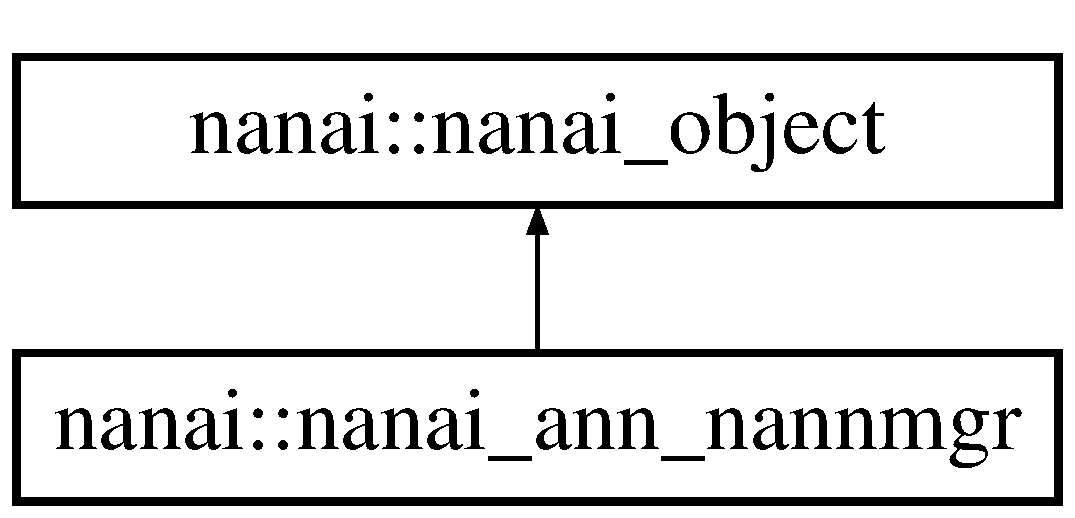
\includegraphics[height=2.000000cm]{classnanai_1_1nanai__ann__nannmgr}
\end{center}
\end{figure}
\subsection*{Public 成员函数}
\begin{DoxyCompactItemize}
\item 
\hyperlink{classnanai_1_1nanai__ann__nannmgr_ac0ab089eae09f4d317218fcad3cfe804}{nanai\+\_\+ann\+\_\+nannmgr} (int max=1024, int now\+\_\+start=0)
\item 
\hyperlink{classnanai_1_1nanai__ann__nannmgr_aa25b7ed3134765348dca37cf200cff3b}{nanai\+\_\+ann\+\_\+nannmgr} (std\+::string alg, \hyperlink{classnanai_1_1nanai__ann__nanncalc_1_1ann__t}{nanai\+\_\+ann\+\_\+nanncalc\+::ann\+\_\+t} \&ann, \hyperlink{classnanmath_1_1nanmath__vector}{nanmath\+::nanmath\+\_\+vector} $\ast$target, int max, int now\+\_\+start)
\item 
virtual \hyperlink{classnanai_1_1nanai__ann__nannmgr_a2594f0a16aed65087e4aebca1b07894e}{$\sim$nanai\+\_\+ann\+\_\+nannmgr} ()
\item 
virtual \hyperlink{classnanai_1_1nanai__ann__nanncalc}{nanai\+\_\+ann\+\_\+nanncalc} $\ast$ \hyperlink{classnanai_1_1nanai__ann__nannmgr_a1b99f051a2a7b2b1ebb21bb45d567afa}{training} (\hyperlink{classnanmath_1_1nanmath__vector}{nanmath\+::nanmath\+\_\+vector} \&input, \hyperlink{classnanmath_1_1nanmath__vector}{nanmath\+::nanmath\+\_\+vector} $\ast$target, \hyperlink{classnanai_1_1nanai__ann__nanncalc}{nanai\+\_\+ann\+\_\+nanncalc} $\ast$dcalc=nullptr, const char $\ast$task=nullptr, \hyperlink{classnanai_1_1nanai__ann__nanncalc_1_1ann__t}{nanai\+\_\+ann\+\_\+nanncalc\+::ann\+\_\+t} $\ast$ann=nullptr, const char $\ast$alg=nullptr)
\item 
virtual \hyperlink{classnanai_1_1nanai__ann__nanncalc}{nanai\+\_\+ann\+\_\+nanncalc} $\ast$ \hyperlink{classnanai_1_1nanai__ann__nannmgr_a7a28db94886caffa0824206c0e2b2fa9}{training\+\_\+notarget} (\hyperlink{classnanmath_1_1nanmath__vector}{nanmath\+::nanmath\+\_\+vector} \&input, \hyperlink{classnanai_1_1nanai__ann__nanncalc}{nanai\+\_\+ann\+\_\+nanncalc} $\ast$dcalc=nullptr, const char $\ast$task=nullptr, \hyperlink{classnanai_1_1nanai__ann__nanncalc_1_1ann__t}{nanai\+\_\+ann\+\_\+nanncalc\+::ann\+\_\+t} $\ast$ann=nullptr, const char $\ast$alg=nullptr)
\item 
virtual \hyperlink{classnanai_1_1nanai__ann__nanncalc}{nanai\+\_\+ann\+\_\+nanncalc} $\ast$ \hyperlink{classnanai_1_1nanai__ann__nannmgr_a7461a5cad561f578869c850adf1e9639}{training\+\_\+nooutput} (\hyperlink{classnanmath_1_1nanmath__vector}{nanmath\+::nanmath\+\_\+vector} \&input, \hyperlink{classnanmath_1_1nanmath__vector}{nanmath\+::nanmath\+\_\+vector} $\ast$target, \hyperlink{classnanai_1_1nanai__ann__nanncalc}{nanai\+\_\+ann\+\_\+nanncalc} $\ast$dcalc=nullptr, const char $\ast$task=nullptr, \hyperlink{classnanai_1_1nanai__ann__nanncalc_1_1ann__t}{nanai\+\_\+ann\+\_\+nanncalc\+::ann\+\_\+t} $\ast$ann=nullptr, const char $\ast$alg=nullptr)
\item 
virtual \hyperlink{classnanai_1_1nanai__ann__nanncalc}{nanai\+\_\+ann\+\_\+nanncalc} $\ast$ \hyperlink{classnanai_1_1nanai__ann__nannmgr_aa4bf6ea43af41a463213c1620757685a}{nnn\+\_\+read} (const std\+::string \&nnn)
\item 
virtual void \hyperlink{classnanai_1_1nanai__ann__nannmgr_a04ac84eff31dab37e338807a4d44d0b9}{nnn\+\_\+write} (const std\+::string \&nnn, \hyperlink{classnanai_1_1nanai__ann__nanncalc}{nanai\+\_\+ann\+\_\+nanncalc} $\ast$calc)
\item 
virtual void \hyperlink{classnanai_1_1nanai__ann__nannmgr_a41e95105ae57bf782fb5ad3b517c4a6a}{waits} ()
\item 
virtual void \hyperlink{classnanai_1_1nanai__ann__nannmgr_ae0a3866bf95574f3d12543da7a326b08}{set\+\_\+max} (int max)
\item 
virtual void \hyperlink{classnanai_1_1nanai__ann__nannmgr_a892c55b5c4a4b22dfd738c1227476ab0}{merge\+\_\+ann\+\_\+by\+\_\+task} (std\+::string task)
\item 
virtual int \hyperlink{classnanai_1_1nanai__ann__nannmgr_a5e88711b173c6074539af3a1b32e761d}{dead\+\_\+task} ()
\item 
virtual int \hyperlink{classnanai_1_1nanai__ann__nannmgr_a1cc1df92755308a610a78c1f16e602c0}{exist\+\_\+task} (std\+::string task)
\end{DoxyCompactItemize}
\subsection*{静态 Public 成员函数}
\begin{DoxyCompactItemize}
\item 
static const char $\ast$ \hyperlink{classnanai_1_1nanai__ann__nannmgr_a94024506784918f4808bbe28c4721335}{version} ()
\end{DoxyCompactItemize}
\subsection*{Protected 成员函数}
\begin{DoxyCompactItemize}
\item 
virtual void \hyperlink{classnanai_1_1nanai__ann__nannmgr_ae4bd257f8c13617deb792e90f72574ea}{init} (int max, int now\+\_\+start)
\item 
virtual \hyperlink{classnanai_1_1nanai__ann__nanncalc_1_1ann__t}{nanai\+\_\+ann\+\_\+nanncalc\+::ann\+\_\+t} \hyperlink{classnanai_1_1nanai__ann__nannmgr_a569b5527d3efd6615b1ed5fe311d3e55}{merge\+\_\+ann} (\hyperlink{classnanai_1_1nanai__ann__nanncalc_1_1ann__t}{nanai\+\_\+ann\+\_\+nanncalc\+::ann\+\_\+t} \&a, \hyperlink{classnanai_1_1nanai__ann__nanncalc_1_1ann__t}{nanai\+\_\+ann\+\_\+nanncalc\+::ann\+\_\+t} \&b)
\item 
virtual \hyperlink{classnanmath_1_1nanmath__matrix}{nanmath\+::nanmath\+\_\+matrix} \hyperlink{classnanai_1_1nanai__ann__nannmgr_a7a9f384ebe727ed9722cbc04e82d30c8}{merge\+\_\+matrix} (\hyperlink{classnanmath_1_1nanmath__matrix}{nanmath\+::nanmath\+\_\+matrix} \&mat1, \hyperlink{classnanmath_1_1nanmath__matrix}{nanmath\+::nanmath\+\_\+matrix} \&mat2, \hyperlink{classnanmath_1_1nanmath__matrix}{nanmath\+::nanmath\+\_\+matrix} \&dmat1, \hyperlink{classnanmath_1_1nanmath__matrix}{nanmath\+::nanmath\+\_\+matrix} \&dmat2)
\item 
virtual \hyperlink{classnanmath_1_1nanmath__matrix}{nanmath\+::nanmath\+\_\+matrix} \hyperlink{classnanai_1_1nanai__ann__nannmgr_a1d9acf82974a0c785349370f40d583af}{merge\+\_\+delta\+\_\+matrix} (\hyperlink{classnanmath_1_1nanmath__matrix}{nanmath\+::nanmath\+\_\+matrix} \&dmat1, \hyperlink{classnanmath_1_1nanmath__matrix}{nanmath\+::nanmath\+\_\+matrix} \&dmat2)
\item 
virtual void \hyperlink{classnanai_1_1nanai__ann__nannmgr_a4097cd6c0d8c9fbd38df08d4474162d7}{configure} ()
\item 
virtual void \hyperlink{classnanai_1_1nanai__ann__nannmgr_a910e51066acc0cefa5a13d441080020a}{get\+\_\+env} ()
\item 
virtual void \hyperlink{classnanai_1_1nanai__ann__nannmgr_af20462056d6628462b18b865197083a5}{get\+\_\+algs} (std\+::string \&path)
\item 
virtual void \hyperlink{classnanai_1_1nanai__ann__nannmgr_a2041f91a11e801557c4e2a310fae4355}{get\+\_\+def\+\_\+algs} ()
\item 
virtual bool \hyperlink{classnanai_1_1nanai__ann__nannmgr_aaf4b292087f8f3f48f6a77140dd512ca}{add\+\_\+alg} (\hyperlink{namespacenanai_a892a8c80381d0005a076b68fbbf2d918}{nanai\+\_\+ann\+\_\+nanndesc} \&desc)
\item 
virtual \hyperlink{namespacenanai_a892a8c80381d0005a076b68fbbf2d918}{nanai\+\_\+ann\+\_\+nanndesc} $\ast$ \hyperlink{classnanai_1_1nanai__ann__nannmgr_aa3fdb4c566c9f8b670631fb559cf1b02}{find\+\_\+alg} (std\+::string alg)
\item 
virtual void \hyperlink{classnanai_1_1nanai__ann__nannmgr_ad67bf88a3df568c5ed07c2adca863be8}{lock} ()
\item 
virtual void \hyperlink{classnanai_1_1nanai__ann__nannmgr_a061504e906faa17ab8cfeccb0f6c17bf}{unlock} ()
\item 
virtual \hyperlink{classnanai_1_1nanai__ann__nanncalc}{nanai\+\_\+ann\+\_\+nanncalc} $\ast$ \hyperlink{classnanai_1_1nanai__ann__nannmgr_a66d329677b38c6d967a737adabaae13e}{generate} (\hyperlink{namespacenanai_a892a8c80381d0005a076b68fbbf2d918}{nanai\+\_\+ann\+\_\+nanndesc} \&desc, \hyperlink{classnanai_1_1nanai__ann__nanncalc_1_1ann__t}{nanai\+\_\+ann\+\_\+nanncalc\+::ann\+\_\+t} $\ast$ann=N\+U\+L\+L, const char $\ast$task=N\+U\+L\+L)
\item 
virtual \hyperlink{classnanai_1_1nanai__ann__nanncalc}{nanai\+\_\+ann\+\_\+nanncalc} $\ast$ \hyperlink{classnanai_1_1nanai__ann__nannmgr_a5f3d6ac53777ccec4d85cde98267693f}{make} (\hyperlink{namespacenanai_a892a8c80381d0005a076b68fbbf2d918}{nanai\+\_\+ann\+\_\+nanndesc} \&desc)
\item 
void \hyperlink{classnanai_1_1nanai__ann__nannmgr_a28ea36058e9dfd5ce6b80d6011931acc}{on\+\_\+error} (int err)
\end{DoxyCompactItemize}
\subsection*{Protected 属性}
\begin{DoxyCompactItemize}
\item 
std\+::string \hyperlink{classnanai_1_1nanai__ann__nannmgr_a8305b13f05cfd2ec029dc325f0921609}{\+\_\+home\+\_\+dir}
\item 
std\+::string \hyperlink{classnanai_1_1nanai__ann__nannmgr_ac074b69306e1ff1a381fbcde3d66d75c}{\+\_\+lib\+\_\+dir}
\item 
std\+::string \hyperlink{classnanai_1_1nanai__ann__nannmgr_a0da1bf8be2e30b97f5414dbba84a9e4c}{\+\_\+etc\+\_\+dir}
\item 
std\+::string \hyperlink{classnanai_1_1nanai__ann__nannmgr_a7d3908d8d93cc40191ec8f20f4808ba0}{\+\_\+log\+\_\+dir}
\item 
std\+::string \hyperlink{classnanai_1_1nanai__ann__nannmgr_a3a14b96819511b38e30bd9857dd86b14}{\+\_\+alg}
\item 
\hyperlink{classnanai_1_1nanai__ann__nanncalc_1_1ann__t}{nanai\+\_\+ann\+\_\+nanncalc\+::ann\+\_\+t} \hyperlink{classnanai_1_1nanai__ann__nannmgr_aa808696e65d0f030afe6e2de2b7d3e6d}{\+\_\+ann}
\item 
\hyperlink{classnanmath_1_1nanmath__vector}{nanmath\+::nanmath\+\_\+vector} \hyperlink{classnanai_1_1nanai__ann__nannmgr_a384127c4c4058bc4b28bdf928d59588a}{\+\_\+target}
\item 
int \hyperlink{classnanai_1_1nanai__ann__nannmgr_a7133133957796b1b5b75e8d761b54866}{\+\_\+max\+\_\+calc}
\item 
int \hyperlink{classnanai_1_1nanai__ann__nannmgr_a8531ad0d6391af0c318f286b44fd0604}{\+\_\+curr\+\_\+calc}
\item 
std\+::vector$<$ \hyperlink{classnanai_1_1nanai__ann__nanncalc}{nanai\+\_\+ann\+\_\+nanncalc} $\ast$ $>$ \hyperlink{classnanai_1_1nanai__ann__nannmgr_a25dc5374ad7545e1c6255afb647264a9}{\+\_\+calcs}
\item 
std\+::vector$<$ \hyperlink{namespacenanai_a892a8c80381d0005a076b68fbbf2d918}{nanai\+\_\+ann\+\_\+nanndesc} $>$ \hyperlink{classnanai_1_1nanai__ann__nannmgr_a4ffd16017f8b8a0aa6dbd0c3210c13d2}{\+\_\+descs}
\item 
std\+::vector$<$ std\+::pair$<$ void $\ast$, \hyperlink{namespacenanai_af358544d3d83ecb56361b1eaa46a0e98}{fptr\+\_\+ann\+\_\+alg\+\_\+setup} $>$ $>$ \hyperlink{classnanai_1_1nanai__ann__nannmgr_a3402ccfa83590793eb0755110e4a023e}{\+\_\+algs}
\item 
pthread\+\_\+mutex\+\_\+t \hyperlink{classnanai_1_1nanai__ann__nannmgr_a9c4963abd61f8aa52b372c01062b5b4d}{\+\_\+lock}
\end{DoxyCompactItemize}


\subsection{详细描述}
南南人工神经网络管理器类 

管理器类用于管理所有计算结点线程 

在文件 nanai\+\_\+ann\+\_\+nannmgr.\+h 第 14 行定义.



\subsection{构造及析构函数说明}
\hypertarget{classnanai_1_1nanai__ann__nannmgr_ac0ab089eae09f4d317218fcad3cfe804}{}\index{nanai\+::nanai\+\_\+ann\+\_\+nannmgr@{nanai\+::nanai\+\_\+ann\+\_\+nannmgr}!nanai\+\_\+ann\+\_\+nannmgr@{nanai\+\_\+ann\+\_\+nannmgr}}
\index{nanai\+\_\+ann\+\_\+nannmgr@{nanai\+\_\+ann\+\_\+nannmgr}!nanai\+::nanai\+\_\+ann\+\_\+nannmgr@{nanai\+::nanai\+\_\+ann\+\_\+nannmgr}}
\subsubsection[{nanai\+\_\+ann\+\_\+nannmgr(int max=1024, int now\+\_\+start=0)}]{\setlength{\rightskip}{0pt plus 5cm}nanai\+::nanai\+\_\+ann\+\_\+nannmgr\+::nanai\+\_\+ann\+\_\+nannmgr (
\begin{DoxyParamCaption}
\item[{int}]{max = {\ttfamily 1024}, }
\item[{int}]{now\+\_\+start = {\ttfamily 0}}
\end{DoxyParamCaption}
)}\label{classnanai_1_1nanai__ann__nannmgr_ac0ab089eae09f4d317218fcad3cfe804}
管理器构造函数. 
\begin{DoxyParams}[1]{参数}
\mbox{\tt in}  & {\em max} & 最大计算结点(线程),默认为1024 \\
\hline
\mbox{\tt in}  & {\em now\+\_\+start} & 当前就要启动的计算结点数 \\
\hline
\end{DoxyParams}


在文件 nanai\+\_\+ann\+\_\+nannmgr.\+cc 第 24 行定义.

\hypertarget{classnanai_1_1nanai__ann__nannmgr_aa25b7ed3134765348dca37cf200cff3b}{}\index{nanai\+::nanai\+\_\+ann\+\_\+nannmgr@{nanai\+::nanai\+\_\+ann\+\_\+nannmgr}!nanai\+\_\+ann\+\_\+nannmgr@{nanai\+\_\+ann\+\_\+nannmgr}}
\index{nanai\+\_\+ann\+\_\+nannmgr@{nanai\+\_\+ann\+\_\+nannmgr}!nanai\+::nanai\+\_\+ann\+\_\+nannmgr@{nanai\+::nanai\+\_\+ann\+\_\+nannmgr}}
\subsubsection[{nanai\+\_\+ann\+\_\+nannmgr(std\+::string alg, nanai\+\_\+ann\+\_\+nanncalc\+::ann\+\_\+t \&ann, nanmath\+::nanmath\+\_\+vector $\ast$target, int max, int now\+\_\+start)}]{\setlength{\rightskip}{0pt plus 5cm}nanai\+::nanai\+\_\+ann\+\_\+nannmgr\+::nanai\+\_\+ann\+\_\+nannmgr (
\begin{DoxyParamCaption}
\item[{std\+::string}]{alg, }
\item[{{\bf nanai\+\_\+ann\+\_\+nanncalc\+::ann\+\_\+t} \&}]{ann, }
\item[{{\bf nanmath\+::nanmath\+\_\+vector} $\ast$}]{target, }
\item[{int}]{max, }
\item[{int}]{now\+\_\+start}
\end{DoxyParamCaption}
)}\label{classnanai_1_1nanai__ann__nannmgr_aa25b7ed3134765348dca37cf200cff3b}
管理器构造函数. 
\begin{DoxyParams}[1]{参数}
\mbox{\tt in}  & {\em alg} & 要设定的神经网络算法 \\
\hline
\mbox{\tt in}  & {\em ann} & 要设定的人工神经网络 \\
\hline
\mbox{\tt in}  & {\em target} & 要训练的目标向量,可选 \\
\hline
\mbox{\tt in}  & {\em max} & 最大计算结点(线程),默认为1024 \\
\hline
\mbox{\tt in}  & {\em now\+\_\+start} & 当前就要启动的计算结点数 \\
\hline
\end{DoxyParams}


在文件 nanai\+\_\+ann\+\_\+nannmgr.\+cc 第 28 行定义.

\hypertarget{classnanai_1_1nanai__ann__nannmgr_a2594f0a16aed65087e4aebca1b07894e}{}\index{nanai\+::nanai\+\_\+ann\+\_\+nannmgr@{nanai\+::nanai\+\_\+ann\+\_\+nannmgr}!````~nanai\+\_\+ann\+\_\+nannmgr@{$\sim$nanai\+\_\+ann\+\_\+nannmgr}}
\index{````~nanai\+\_\+ann\+\_\+nannmgr@{$\sim$nanai\+\_\+ann\+\_\+nannmgr}!nanai\+::nanai\+\_\+ann\+\_\+nannmgr@{nanai\+::nanai\+\_\+ann\+\_\+nannmgr}}
\subsubsection[{$\sim$nanai\+\_\+ann\+\_\+nannmgr()}]{\setlength{\rightskip}{0pt plus 5cm}nanai\+::nanai\+\_\+ann\+\_\+nannmgr\+::$\sim$nanai\+\_\+ann\+\_\+nannmgr (
\begin{DoxyParamCaption}
{}
\end{DoxyParamCaption}
)\hspace{0.3cm}{\ttfamily [virtual]}}\label{classnanai_1_1nanai__ann__nannmgr_a2594f0a16aed65087e4aebca1b07894e}
析构函数.

会向所有正在工作的线程发出停止的命令,并等待完成,最后销毁 

在文件 nanai\+\_\+ann\+\_\+nannmgr.\+cc 第 40 行定义.



\subsection{成员函数说明}
\hypertarget{classnanai_1_1nanai__ann__nannmgr_aaf4b292087f8f3f48f6a77140dd512ca}{}\index{nanai\+::nanai\+\_\+ann\+\_\+nannmgr@{nanai\+::nanai\+\_\+ann\+\_\+nannmgr}!add\+\_\+alg@{add\+\_\+alg}}
\index{add\+\_\+alg@{add\+\_\+alg}!nanai\+::nanai\+\_\+ann\+\_\+nannmgr@{nanai\+::nanai\+\_\+ann\+\_\+nannmgr}}
\subsubsection[{add\+\_\+alg(nanai\+\_\+ann\+\_\+nanndesc \&desc)}]{\setlength{\rightskip}{0pt plus 5cm}bool nanai\+::nanai\+\_\+ann\+\_\+nannmgr\+::add\+\_\+alg (
\begin{DoxyParamCaption}
\item[{{\bf nanai\+\_\+ann\+\_\+nanndesc} \&}]{desc}
\end{DoxyParamCaption}
)\hspace{0.3cm}{\ttfamily [protected]}, {\ttfamily [virtual]}}\label{classnanai_1_1nanai__ann__nannmgr_aaf4b292087f8f3f48f6a77140dd512ca}


在文件 nanai\+\_\+ann\+\_\+nannmgr.\+cc 第 530 行定义.

\hypertarget{classnanai_1_1nanai__ann__nannmgr_a4097cd6c0d8c9fbd38df08d4474162d7}{}\index{nanai\+::nanai\+\_\+ann\+\_\+nannmgr@{nanai\+::nanai\+\_\+ann\+\_\+nannmgr}!configure@{configure}}
\index{configure@{configure}!nanai\+::nanai\+\_\+ann\+\_\+nannmgr@{nanai\+::nanai\+\_\+ann\+\_\+nannmgr}}
\subsubsection[{configure()}]{\setlength{\rightskip}{0pt plus 5cm}void nanai\+::nanai\+\_\+ann\+\_\+nannmgr\+::configure (
\begin{DoxyParamCaption}
{}
\end{DoxyParamCaption}
)\hspace{0.3cm}{\ttfamily [protected]}, {\ttfamily [virtual]}}\label{classnanai_1_1nanai__ann__nannmgr_a4097cd6c0d8c9fbd38df08d4474162d7}


在文件 nanai\+\_\+ann\+\_\+nannmgr.\+cc 第 428 行定义.

\hypertarget{classnanai_1_1nanai__ann__nannmgr_a5e88711b173c6074539af3a1b32e761d}{}\index{nanai\+::nanai\+\_\+ann\+\_\+nannmgr@{nanai\+::nanai\+\_\+ann\+\_\+nannmgr}!dead\+\_\+task@{dead\+\_\+task}}
\index{dead\+\_\+task@{dead\+\_\+task}!nanai\+::nanai\+\_\+ann\+\_\+nannmgr@{nanai\+::nanai\+\_\+ann\+\_\+nannmgr}}
\subsubsection[{dead\+\_\+task()}]{\setlength{\rightskip}{0pt plus 5cm}int nanai\+::nanai\+\_\+ann\+\_\+nannmgr\+::dead\+\_\+task (
\begin{DoxyParamCaption}
{}
\end{DoxyParamCaption}
)\hspace{0.3cm}{\ttfamily [virtual]}}\label{classnanai_1_1nanai__ann__nannmgr_a5e88711b173c6074539af3a1b32e761d}


在文件 nanai\+\_\+ann\+\_\+nannmgr.\+cc 第 295 行定义.

\hypertarget{classnanai_1_1nanai__ann__nannmgr_a1cc1df92755308a610a78c1f16e602c0}{}\index{nanai\+::nanai\+\_\+ann\+\_\+nannmgr@{nanai\+::nanai\+\_\+ann\+\_\+nannmgr}!exist\+\_\+task@{exist\+\_\+task}}
\index{exist\+\_\+task@{exist\+\_\+task}!nanai\+::nanai\+\_\+ann\+\_\+nannmgr@{nanai\+::nanai\+\_\+ann\+\_\+nannmgr}}
\subsubsection[{exist\+\_\+task(std\+::string task)}]{\setlength{\rightskip}{0pt plus 5cm}int nanai\+::nanai\+\_\+ann\+\_\+nannmgr\+::exist\+\_\+task (
\begin{DoxyParamCaption}
\item[{std\+::string}]{task}
\end{DoxyParamCaption}
)\hspace{0.3cm}{\ttfamily [virtual]}}\label{classnanai_1_1nanai__ann__nannmgr_a1cc1df92755308a610a78c1f16e602c0}


在文件 nanai\+\_\+ann\+\_\+nannmgr.\+cc 第 277 行定义.

\hypertarget{classnanai_1_1nanai__ann__nannmgr_aa3fdb4c566c9f8b670631fb559cf1b02}{}\index{nanai\+::nanai\+\_\+ann\+\_\+nannmgr@{nanai\+::nanai\+\_\+ann\+\_\+nannmgr}!find\+\_\+alg@{find\+\_\+alg}}
\index{find\+\_\+alg@{find\+\_\+alg}!nanai\+::nanai\+\_\+ann\+\_\+nannmgr@{nanai\+::nanai\+\_\+ann\+\_\+nannmgr}}
\subsubsection[{find\+\_\+alg(std\+::string alg)}]{\setlength{\rightskip}{0pt plus 5cm}{\bf nanai\+\_\+ann\+\_\+nanndesc} $\ast$ nanai\+::nanai\+\_\+ann\+\_\+nannmgr\+::find\+\_\+alg (
\begin{DoxyParamCaption}
\item[{std\+::string}]{alg}
\end{DoxyParamCaption}
)\hspace{0.3cm}{\ttfamily [protected]}, {\ttfamily [virtual]}}\label{classnanai_1_1nanai__ann__nannmgr_aa3fdb4c566c9f8b670631fb559cf1b02}


在文件 nanai\+\_\+ann\+\_\+nannmgr.\+cc 第 546 行定义.

\hypertarget{classnanai_1_1nanai__ann__nannmgr_a66d329677b38c6d967a737adabaae13e}{}\index{nanai\+::nanai\+\_\+ann\+\_\+nannmgr@{nanai\+::nanai\+\_\+ann\+\_\+nannmgr}!generate@{generate}}
\index{generate@{generate}!nanai\+::nanai\+\_\+ann\+\_\+nannmgr@{nanai\+::nanai\+\_\+ann\+\_\+nannmgr}}
\subsubsection[{generate(nanai\+\_\+ann\+\_\+nanndesc \&desc, nanai\+\_\+ann\+\_\+nanncalc\+::ann\+\_\+t $\ast$ann=\+N\+U\+L\+L, const char $\ast$task=\+N\+U\+L\+L)}]{\setlength{\rightskip}{0pt plus 5cm}{\bf nanai\+\_\+ann\+\_\+nanncalc} $\ast$ nanai\+::nanai\+\_\+ann\+\_\+nannmgr\+::generate (
\begin{DoxyParamCaption}
\item[{{\bf nanai\+\_\+ann\+\_\+nanndesc} \&}]{desc, }
\item[{{\bf nanai\+\_\+ann\+\_\+nanncalc\+::ann\+\_\+t} $\ast$}]{ann = {\ttfamily NULL}, }
\item[{const char $\ast$}]{task = {\ttfamily NULL}}
\end{DoxyParamCaption}
)\hspace{0.3cm}{\ttfamily [protected]}, {\ttfamily [virtual]}}\label{classnanai_1_1nanai__ann__nannmgr_a66d329677b38c6d967a737adabaae13e}


在文件 nanai\+\_\+ann\+\_\+nannmgr.\+cc 第 568 行定义.

\hypertarget{classnanai_1_1nanai__ann__nannmgr_af20462056d6628462b18b865197083a5}{}\index{nanai\+::nanai\+\_\+ann\+\_\+nannmgr@{nanai\+::nanai\+\_\+ann\+\_\+nannmgr}!get\+\_\+algs@{get\+\_\+algs}}
\index{get\+\_\+algs@{get\+\_\+algs}!nanai\+::nanai\+\_\+ann\+\_\+nannmgr@{nanai\+::nanai\+\_\+ann\+\_\+nannmgr}}
\subsubsection[{get\+\_\+algs(std\+::string \&path)}]{\setlength{\rightskip}{0pt plus 5cm}void nanai\+::nanai\+\_\+ann\+\_\+nannmgr\+::get\+\_\+algs (
\begin{DoxyParamCaption}
\item[{std\+::string \&}]{path}
\end{DoxyParamCaption}
)\hspace{0.3cm}{\ttfamily [protected]}, {\ttfamily [virtual]}}\label{classnanai_1_1nanai__ann__nannmgr_af20462056d6628462b18b865197083a5}


在文件 nanai\+\_\+ann\+\_\+nannmgr.\+cc 第 479 行定义.

\hypertarget{classnanai_1_1nanai__ann__nannmgr_a2041f91a11e801557c4e2a310fae4355}{}\index{nanai\+::nanai\+\_\+ann\+\_\+nannmgr@{nanai\+::nanai\+\_\+ann\+\_\+nannmgr}!get\+\_\+def\+\_\+algs@{get\+\_\+def\+\_\+algs}}
\index{get\+\_\+def\+\_\+algs@{get\+\_\+def\+\_\+algs}!nanai\+::nanai\+\_\+ann\+\_\+nannmgr@{nanai\+::nanai\+\_\+ann\+\_\+nannmgr}}
\subsubsection[{get\+\_\+def\+\_\+algs()}]{\setlength{\rightskip}{0pt plus 5cm}void nanai\+::nanai\+\_\+ann\+\_\+nannmgr\+::get\+\_\+def\+\_\+algs (
\begin{DoxyParamCaption}
{}
\end{DoxyParamCaption}
)\hspace{0.3cm}{\ttfamily [protected]}, {\ttfamily [virtual]}}\label{classnanai_1_1nanai__ann__nannmgr_a2041f91a11e801557c4e2a310fae4355}


在文件 nanai\+\_\+ann\+\_\+nannmgr.\+cc 第 525 行定义.

\hypertarget{classnanai_1_1nanai__ann__nannmgr_a910e51066acc0cefa5a13d441080020a}{}\index{nanai\+::nanai\+\_\+ann\+\_\+nannmgr@{nanai\+::nanai\+\_\+ann\+\_\+nannmgr}!get\+\_\+env@{get\+\_\+env}}
\index{get\+\_\+env@{get\+\_\+env}!nanai\+::nanai\+\_\+ann\+\_\+nannmgr@{nanai\+::nanai\+\_\+ann\+\_\+nannmgr}}
\subsubsection[{get\+\_\+env()}]{\setlength{\rightskip}{0pt plus 5cm}void nanai\+::nanai\+\_\+ann\+\_\+nannmgr\+::get\+\_\+env (
\begin{DoxyParamCaption}
{}
\end{DoxyParamCaption}
)\hspace{0.3cm}{\ttfamily [protected]}, {\ttfamily [virtual]}}\label{classnanai_1_1nanai__ann__nannmgr_a910e51066acc0cefa5a13d441080020a}


在文件 nanai\+\_\+ann\+\_\+nannmgr.\+cc 第 443 行定义.

\hypertarget{classnanai_1_1nanai__ann__nannmgr_ae4bd257f8c13617deb792e90f72574ea}{}\index{nanai\+::nanai\+\_\+ann\+\_\+nannmgr@{nanai\+::nanai\+\_\+ann\+\_\+nannmgr}!init@{init}}
\index{init@{init}!nanai\+::nanai\+\_\+ann\+\_\+nannmgr@{nanai\+::nanai\+\_\+ann\+\_\+nannmgr}}
\subsubsection[{init(int max, int now\+\_\+start)}]{\setlength{\rightskip}{0pt plus 5cm}void nanai\+::nanai\+\_\+ann\+\_\+nannmgr\+::init (
\begin{DoxyParamCaption}
\item[{int}]{max, }
\item[{int}]{now\+\_\+start}
\end{DoxyParamCaption}
)\hspace{0.3cm}{\ttfamily [protected]}, {\ttfamily [virtual]}}\label{classnanai_1_1nanai__ann__nannmgr_ae4bd257f8c13617deb792e90f72574ea}
初始化所有的数据. 
\begin{DoxyParams}[1]{参数}
\mbox{\tt in}  & {\em max} & 最大计算结点(线程),默认为1024 \\
\hline
\mbox{\tt in}  & {\em now\+\_\+start} & 当前就要启动的计算结点数 \\
\hline
\end{DoxyParams}


在文件 nanai\+\_\+ann\+\_\+nannmgr.\+cc 第 58 行定义.

\hypertarget{classnanai_1_1nanai__ann__nannmgr_ad67bf88a3df568c5ed07c2adca863be8}{}\index{nanai\+::nanai\+\_\+ann\+\_\+nannmgr@{nanai\+::nanai\+\_\+ann\+\_\+nannmgr}!lock@{lock}}
\index{lock@{lock}!nanai\+::nanai\+\_\+ann\+\_\+nannmgr@{nanai\+::nanai\+\_\+ann\+\_\+nannmgr}}
\subsubsection[{lock()}]{\setlength{\rightskip}{0pt plus 5cm}void nanai\+::nanai\+\_\+ann\+\_\+nannmgr\+::lock (
\begin{DoxyParamCaption}
{}
\end{DoxyParamCaption}
)\hspace{0.3cm}{\ttfamily [protected]}, {\ttfamily [virtual]}}\label{classnanai_1_1nanai__ann__nannmgr_ad67bf88a3df568c5ed07c2adca863be8}


在文件 nanai\+\_\+ann\+\_\+nannmgr.\+cc 第 556 行定义.

\hypertarget{classnanai_1_1nanai__ann__nannmgr_a5f3d6ac53777ccec4d85cde98267693f}{}\index{nanai\+::nanai\+\_\+ann\+\_\+nannmgr@{nanai\+::nanai\+\_\+ann\+\_\+nannmgr}!make@{make}}
\index{make@{make}!nanai\+::nanai\+\_\+ann\+\_\+nannmgr@{nanai\+::nanai\+\_\+ann\+\_\+nannmgr}}
\subsubsection[{make(nanai\+\_\+ann\+\_\+nanndesc \&desc)}]{\setlength{\rightskip}{0pt plus 5cm}{\bf nanai\+\_\+ann\+\_\+nanncalc} $\ast$ nanai\+::nanai\+\_\+ann\+\_\+nannmgr\+::make (
\begin{DoxyParamCaption}
\item[{{\bf nanai\+\_\+ann\+\_\+nanndesc} \&}]{desc}
\end{DoxyParamCaption}
)\hspace{0.3cm}{\ttfamily [protected]}, {\ttfamily [virtual]}}\label{classnanai_1_1nanai__ann__nannmgr_a5f3d6ac53777ccec4d85cde98267693f}


在文件 nanai\+\_\+ann\+\_\+nannmgr.\+cc 第 637 行定义.

\hypertarget{classnanai_1_1nanai__ann__nannmgr_a569b5527d3efd6615b1ed5fe311d3e55}{}\index{nanai\+::nanai\+\_\+ann\+\_\+nannmgr@{nanai\+::nanai\+\_\+ann\+\_\+nannmgr}!merge\+\_\+ann@{merge\+\_\+ann}}
\index{merge\+\_\+ann@{merge\+\_\+ann}!nanai\+::nanai\+\_\+ann\+\_\+nannmgr@{nanai\+::nanai\+\_\+ann\+\_\+nannmgr}}
\subsubsection[{merge\+\_\+ann(nanai\+\_\+ann\+\_\+nanncalc\+::ann\+\_\+t \&a, nanai\+\_\+ann\+\_\+nanncalc\+::ann\+\_\+t \&b)}]{\setlength{\rightskip}{0pt plus 5cm}{\bf nanai\+\_\+ann\+\_\+nanncalc\+::ann\+\_\+t} nanai\+::nanai\+\_\+ann\+\_\+nannmgr\+::merge\+\_\+ann (
\begin{DoxyParamCaption}
\item[{{\bf nanai\+\_\+ann\+\_\+nanncalc\+::ann\+\_\+t} \&}]{a, }
\item[{{\bf nanai\+\_\+ann\+\_\+nanncalc\+::ann\+\_\+t} \&}]{b}
\end{DoxyParamCaption}
)\hspace{0.3cm}{\ttfamily [protected]}, {\ttfamily [virtual]}}\label{classnanai_1_1nanai__ann__nannmgr_a569b5527d3efd6615b1ed5fe311d3e55}


在文件 nanai\+\_\+ann\+\_\+nannmgr.\+cc 第 371 行定义.

\hypertarget{classnanai_1_1nanai__ann__nannmgr_a892c55b5c4a4b22dfd738c1227476ab0}{}\index{nanai\+::nanai\+\_\+ann\+\_\+nannmgr@{nanai\+::nanai\+\_\+ann\+\_\+nannmgr}!merge\+\_\+ann\+\_\+by\+\_\+task@{merge\+\_\+ann\+\_\+by\+\_\+task}}
\index{merge\+\_\+ann\+\_\+by\+\_\+task@{merge\+\_\+ann\+\_\+by\+\_\+task}!nanai\+::nanai\+\_\+ann\+\_\+nannmgr@{nanai\+::nanai\+\_\+ann\+\_\+nannmgr}}
\subsubsection[{merge\+\_\+ann\+\_\+by\+\_\+task(std\+::string task)}]{\setlength{\rightskip}{0pt plus 5cm}void nanai\+::nanai\+\_\+ann\+\_\+nannmgr\+::merge\+\_\+ann\+\_\+by\+\_\+task (
\begin{DoxyParamCaption}
\item[{std\+::string}]{task}
\end{DoxyParamCaption}
)\hspace{0.3cm}{\ttfamily [virtual]}}\label{classnanai_1_1nanai__ann__nannmgr_a892c55b5c4a4b22dfd738c1227476ab0}


在文件 nanai\+\_\+ann\+\_\+nannmgr.\+cc 第 398 行定义.

\hypertarget{classnanai_1_1nanai__ann__nannmgr_a1d9acf82974a0c785349370f40d583af}{}\index{nanai\+::nanai\+\_\+ann\+\_\+nannmgr@{nanai\+::nanai\+\_\+ann\+\_\+nannmgr}!merge\+\_\+delta\+\_\+matrix@{merge\+\_\+delta\+\_\+matrix}}
\index{merge\+\_\+delta\+\_\+matrix@{merge\+\_\+delta\+\_\+matrix}!nanai\+::nanai\+\_\+ann\+\_\+nannmgr@{nanai\+::nanai\+\_\+ann\+\_\+nannmgr}}
\subsubsection[{merge\+\_\+delta\+\_\+matrix(nanmath\+::nanmath\+\_\+matrix \&dmat1, nanmath\+::nanmath\+\_\+matrix \&dmat2)}]{\setlength{\rightskip}{0pt plus 5cm}{\bf nanmath\+::nanmath\+\_\+matrix} nanai\+::nanai\+\_\+ann\+\_\+nannmgr\+::merge\+\_\+delta\+\_\+matrix (
\begin{DoxyParamCaption}
\item[{{\bf nanmath\+::nanmath\+\_\+matrix} \&}]{dmat1, }
\item[{{\bf nanmath\+::nanmath\+\_\+matrix} \&}]{dmat2}
\end{DoxyParamCaption}
)\hspace{0.3cm}{\ttfamily [protected]}, {\ttfamily [virtual]}}\label{classnanai_1_1nanai__ann__nannmgr_a1d9acf82974a0c785349370f40d583af}


在文件 nanai\+\_\+ann\+\_\+nannmgr.\+cc 第 313 行定义.

\hypertarget{classnanai_1_1nanai__ann__nannmgr_a7a9f384ebe727ed9722cbc04e82d30c8}{}\index{nanai\+::nanai\+\_\+ann\+\_\+nannmgr@{nanai\+::nanai\+\_\+ann\+\_\+nannmgr}!merge\+\_\+matrix@{merge\+\_\+matrix}}
\index{merge\+\_\+matrix@{merge\+\_\+matrix}!nanai\+::nanai\+\_\+ann\+\_\+nannmgr@{nanai\+::nanai\+\_\+ann\+\_\+nannmgr}}
\subsubsection[{merge\+\_\+matrix(nanmath\+::nanmath\+\_\+matrix \&mat1, nanmath\+::nanmath\+\_\+matrix \&mat2, nanmath\+::nanmath\+\_\+matrix \&dmat1, nanmath\+::nanmath\+\_\+matrix \&dmat2)}]{\setlength{\rightskip}{0pt plus 5cm}{\bf nanmath\+::nanmath\+\_\+matrix} nanai\+::nanai\+\_\+ann\+\_\+nannmgr\+::merge\+\_\+matrix (
\begin{DoxyParamCaption}
\item[{{\bf nanmath\+::nanmath\+\_\+matrix} \&}]{mat1, }
\item[{{\bf nanmath\+::nanmath\+\_\+matrix} \&}]{mat2, }
\item[{{\bf nanmath\+::nanmath\+\_\+matrix} \&}]{dmat1, }
\item[{{\bf nanmath\+::nanmath\+\_\+matrix} \&}]{dmat2}
\end{DoxyParamCaption}
)\hspace{0.3cm}{\ttfamily [protected]}, {\ttfamily [virtual]}}\label{classnanai_1_1nanai__ann__nannmgr_a7a9f384ebe727ed9722cbc04e82d30c8}


在文件 nanai\+\_\+ann\+\_\+nannmgr.\+cc 第 339 行定义.

\hypertarget{classnanai_1_1nanai__ann__nannmgr_aa4bf6ea43af41a463213c1620757685a}{}\index{nanai\+::nanai\+\_\+ann\+\_\+nannmgr@{nanai\+::nanai\+\_\+ann\+\_\+nannmgr}!nnn\+\_\+read@{nnn\+\_\+read}}
\index{nnn\+\_\+read@{nnn\+\_\+read}!nanai\+::nanai\+\_\+ann\+\_\+nannmgr@{nanai\+::nanai\+\_\+ann\+\_\+nannmgr}}
\subsubsection[{nnn\+\_\+read(const std\+::string \&nnn)}]{\setlength{\rightskip}{0pt plus 5cm}{\bf nanai\+\_\+ann\+\_\+nanncalc} $\ast$ nanai\+::nanai\+\_\+ann\+\_\+nannmgr\+::nnn\+\_\+read (
\begin{DoxyParamCaption}
\item[{const std\+::string \&}]{nnn}
\end{DoxyParamCaption}
)\hspace{0.3cm}{\ttfamily [virtual]}}\label{classnanai_1_1nanai__ann__nannmgr_aa4bf6ea43af41a463213c1620757685a}


在文件 nanai\+\_\+ann\+\_\+nannmgr.\+cc 第 196 行定义.

\hypertarget{classnanai_1_1nanai__ann__nannmgr_a04ac84eff31dab37e338807a4d44d0b9}{}\index{nanai\+::nanai\+\_\+ann\+\_\+nannmgr@{nanai\+::nanai\+\_\+ann\+\_\+nannmgr}!nnn\+\_\+write@{nnn\+\_\+write}}
\index{nnn\+\_\+write@{nnn\+\_\+write}!nanai\+::nanai\+\_\+ann\+\_\+nannmgr@{nanai\+::nanai\+\_\+ann\+\_\+nannmgr}}
\subsubsection[{nnn\+\_\+write(const std\+::string \&nnn, nanai\+\_\+ann\+\_\+nanncalc $\ast$calc)}]{\setlength{\rightskip}{0pt plus 5cm}void nanai\+::nanai\+\_\+ann\+\_\+nannmgr\+::nnn\+\_\+write (
\begin{DoxyParamCaption}
\item[{const std\+::string \&}]{nnn, }
\item[{{\bf nanai\+\_\+ann\+\_\+nanncalc} $\ast$}]{calc}
\end{DoxyParamCaption}
)\hspace{0.3cm}{\ttfamily [virtual]}}\label{classnanai_1_1nanai__ann__nannmgr_a04ac84eff31dab37e338807a4d44d0b9}


在文件 nanai\+\_\+ann\+\_\+nannmgr.\+cc 第 235 行定义.

\hypertarget{classnanai_1_1nanai__ann__nannmgr_a28ea36058e9dfd5ce6b80d6011931acc}{}\index{nanai\+::nanai\+\_\+ann\+\_\+nannmgr@{nanai\+::nanai\+\_\+ann\+\_\+nannmgr}!on\+\_\+error@{on\+\_\+error}}
\index{on\+\_\+error@{on\+\_\+error}!nanai\+::nanai\+\_\+ann\+\_\+nannmgr@{nanai\+::nanai\+\_\+ann\+\_\+nannmgr}}
\subsubsection[{on\+\_\+error(int err)}]{\setlength{\rightskip}{0pt plus 5cm}void nanai\+::nanai\+\_\+ann\+\_\+nannmgr\+::on\+\_\+error (
\begin{DoxyParamCaption}
\item[{int}]{err}
\end{DoxyParamCaption}
)\hspace{0.3cm}{\ttfamily [protected]}, {\ttfamily [virtual]}}\label{classnanai_1_1nanai__ann__nannmgr_a28ea36058e9dfd5ce6b80d6011931acc}


重载 \hyperlink{classnanai_1_1nanai__object_a87f162335cead23a1409f7c0570a3284}{nanai\+::nanai\+\_\+object} .



在文件 nanai\+\_\+ann\+\_\+nannmgr.\+cc 第 646 行定义.

\hypertarget{classnanai_1_1nanai__ann__nannmgr_ae0a3866bf95574f3d12543da7a326b08}{}\index{nanai\+::nanai\+\_\+ann\+\_\+nannmgr@{nanai\+::nanai\+\_\+ann\+\_\+nannmgr}!set\+\_\+max@{set\+\_\+max}}
\index{set\+\_\+max@{set\+\_\+max}!nanai\+::nanai\+\_\+ann\+\_\+nannmgr@{nanai\+::nanai\+\_\+ann\+\_\+nannmgr}}
\subsubsection[{set\+\_\+max(int max)}]{\setlength{\rightskip}{0pt plus 5cm}void nanai\+::nanai\+\_\+ann\+\_\+nannmgr\+::set\+\_\+max (
\begin{DoxyParamCaption}
\item[{int}]{max}
\end{DoxyParamCaption}
)\hspace{0.3cm}{\ttfamily [virtual]}}\label{classnanai_1_1nanai__ann__nannmgr_ae0a3866bf95574f3d12543da7a326b08}


在文件 nanai\+\_\+ann\+\_\+nannmgr.\+cc 第 309 行定义.

\hypertarget{classnanai_1_1nanai__ann__nannmgr_a1b99f051a2a7b2b1ebb21bb45d567afa}{}\index{nanai\+::nanai\+\_\+ann\+\_\+nannmgr@{nanai\+::nanai\+\_\+ann\+\_\+nannmgr}!training@{training}}
\index{training@{training}!nanai\+::nanai\+\_\+ann\+\_\+nannmgr@{nanai\+::nanai\+\_\+ann\+\_\+nannmgr}}
\subsubsection[{training(nanmath\+::nanmath\+\_\+vector \&input, nanmath\+::nanmath\+\_\+vector $\ast$target, nanai\+\_\+ann\+\_\+nanncalc $\ast$dcalc=nullptr, const char $\ast$task=nullptr, nanai\+\_\+ann\+\_\+nanncalc\+::ann\+\_\+t $\ast$ann=nullptr, const char $\ast$alg=nullptr)}]{\setlength{\rightskip}{0pt plus 5cm}{\bf nanai\+\_\+ann\+\_\+nanncalc} $\ast$ nanai\+::nanai\+\_\+ann\+\_\+nannmgr\+::training (
\begin{DoxyParamCaption}
\item[{{\bf nanmath\+::nanmath\+\_\+vector} \&}]{input, }
\item[{{\bf nanmath\+::nanmath\+\_\+vector} $\ast$}]{target, }
\item[{{\bf nanai\+\_\+ann\+\_\+nanncalc} $\ast$}]{dcalc = {\ttfamily nullptr}, }
\item[{const char $\ast$}]{task = {\ttfamily nullptr}, }
\item[{{\bf nanai\+\_\+ann\+\_\+nanncalc\+::ann\+\_\+t} $\ast$}]{ann = {\ttfamily nullptr}, }
\item[{const char $\ast$}]{alg = {\ttfamily nullptr}}
\end{DoxyParamCaption}
)\hspace{0.3cm}{\ttfamily [virtual]}}\label{classnanai_1_1nanai__ann__nannmgr_a1b99f051a2a7b2b1ebb21bb45d567afa}
输出结果,并调整误差

如果指定的计算结点dcalc不为空,则直接使用,随后判断是否指定了算法alg。如果指定了则通过alg 寻找算法描述结点,如果没有找打则抛出异常“\+N\+A\+N\+A\+I\+\_\+\+E\+R\+R\+O\+R\+\_\+\+L\+O\+G\+I\+C\+\_\+\+A\+L\+G\+\_\+\+N\+O\+T\+\_\+\+F\+O\+U\+N\+D”。找到了则 修改当前dcalc计算结点的配置为算法alg的描述结点。如果指定了ann,则应用。如果指定了target 则应用当前指定的目标向量,如果没有指定则使用默认的目标向量。

如果没有指定计算结点,首先会通过alg参数寻找当前管理器是否加载对应的算法描述插件,没有则抛出 “\+N\+A\+N\+A\+I\+\_\+\+E\+R\+R\+O\+R\+\_\+\+L\+O\+G\+I\+C\+\_\+\+A\+L\+G\+\_\+\+N\+O\+T\+\_\+\+F\+O\+U\+N\+D”,如果找到,则调用generate产生一个新的计算结点来进行 训练。如果指定了target则应用当前指定的目标向量,如果没有指定则使用默认的目标向量。 
\begin{DoxyParams}[1]{参数}
\mbox{\tt in}  & {\em input} & 输入样本向量 \\
\hline
\mbox{\tt in}  & {\em target} & 训练目标向量,可选 \\
\hline
\mbox{\tt in}  & {\em dcalc} & 要直接使用的计算结点,可选 \\
\hline
\mbox{\tt in}  & {\em task} & 任务的名称,可选 \\
\hline
\mbox{\tt in}  & {\em ann} & 人工神经网络,可选 \\
\hline
\mbox{\tt in}  & {\em alg} & 可选用的算法,可选 \\
\hline
\end{DoxyParams}


在文件 nanai\+\_\+ann\+\_\+nannmgr.\+cc 第 78 行定义.

\hypertarget{classnanai_1_1nanai__ann__nannmgr_a7461a5cad561f578869c850adf1e9639}{}\index{nanai\+::nanai\+\_\+ann\+\_\+nannmgr@{nanai\+::nanai\+\_\+ann\+\_\+nannmgr}!training\+\_\+nooutput@{training\+\_\+nooutput}}
\index{training\+\_\+nooutput@{training\+\_\+nooutput}!nanai\+::nanai\+\_\+ann\+\_\+nannmgr@{nanai\+::nanai\+\_\+ann\+\_\+nannmgr}}
\subsubsection[{training\+\_\+nooutput(nanmath\+::nanmath\+\_\+vector \&input, nanmath\+::nanmath\+\_\+vector $\ast$target, nanai\+\_\+ann\+\_\+nanncalc $\ast$dcalc=nullptr, const char $\ast$task=nullptr, nanai\+\_\+ann\+\_\+nanncalc\+::ann\+\_\+t $\ast$ann=nullptr, const char $\ast$alg=nullptr)}]{\setlength{\rightskip}{0pt plus 5cm}{\bf nanai\+\_\+ann\+\_\+nanncalc} $\ast$ nanai\+::nanai\+\_\+ann\+\_\+nannmgr\+::training\+\_\+nooutput (
\begin{DoxyParamCaption}
\item[{{\bf nanmath\+::nanmath\+\_\+vector} \&}]{input, }
\item[{{\bf nanmath\+::nanmath\+\_\+vector} $\ast$}]{target, }
\item[{{\bf nanai\+\_\+ann\+\_\+nanncalc} $\ast$}]{dcalc = {\ttfamily nullptr}, }
\item[{const char $\ast$}]{task = {\ttfamily nullptr}, }
\item[{{\bf nanai\+\_\+ann\+\_\+nanncalc\+::ann\+\_\+t} $\ast$}]{ann = {\ttfamily nullptr}, }
\item[{const char $\ast$}]{alg = {\ttfamily nullptr}}
\end{DoxyParamCaption}
)\hspace{0.3cm}{\ttfamily [virtual]}}\label{classnanai_1_1nanai__ann__nannmgr_a7461a5cad561f578869c850adf1e9639}


在文件 nanai\+\_\+ann\+\_\+nannmgr.\+cc 第 157 行定义.

\hypertarget{classnanai_1_1nanai__ann__nannmgr_a7a28db94886caffa0824206c0e2b2fa9}{}\index{nanai\+::nanai\+\_\+ann\+\_\+nannmgr@{nanai\+::nanai\+\_\+ann\+\_\+nannmgr}!training\+\_\+notarget@{training\+\_\+notarget}}
\index{training\+\_\+notarget@{training\+\_\+notarget}!nanai\+::nanai\+\_\+ann\+\_\+nannmgr@{nanai\+::nanai\+\_\+ann\+\_\+nannmgr}}
\subsubsection[{training\+\_\+notarget(nanmath\+::nanmath\+\_\+vector \&input, nanai\+\_\+ann\+\_\+nanncalc $\ast$dcalc=nullptr, const char $\ast$task=nullptr, nanai\+\_\+ann\+\_\+nanncalc\+::ann\+\_\+t $\ast$ann=nullptr, const char $\ast$alg=nullptr)}]{\setlength{\rightskip}{0pt plus 5cm}{\bf nanai\+\_\+ann\+\_\+nanncalc} $\ast$ nanai\+::nanai\+\_\+ann\+\_\+nannmgr\+::training\+\_\+notarget (
\begin{DoxyParamCaption}
\item[{{\bf nanmath\+::nanmath\+\_\+vector} \&}]{input, }
\item[{{\bf nanai\+\_\+ann\+\_\+nanncalc} $\ast$}]{dcalc = {\ttfamily nullptr}, }
\item[{const char $\ast$}]{task = {\ttfamily nullptr}, }
\item[{{\bf nanai\+\_\+ann\+\_\+nanncalc\+::ann\+\_\+t} $\ast$}]{ann = {\ttfamily nullptr}, }
\item[{const char $\ast$}]{alg = {\ttfamily nullptr}}
\end{DoxyParamCaption}
)\hspace{0.3cm}{\ttfamily [virtual]}}\label{classnanai_1_1nanai__ann__nannmgr_a7a28db94886caffa0824206c0e2b2fa9}


在文件 nanai\+\_\+ann\+\_\+nannmgr.\+cc 第 124 行定义.

\hypertarget{classnanai_1_1nanai__ann__nannmgr_a061504e906faa17ab8cfeccb0f6c17bf}{}\index{nanai\+::nanai\+\_\+ann\+\_\+nannmgr@{nanai\+::nanai\+\_\+ann\+\_\+nannmgr}!unlock@{unlock}}
\index{unlock@{unlock}!nanai\+::nanai\+\_\+ann\+\_\+nannmgr@{nanai\+::nanai\+\_\+ann\+\_\+nannmgr}}
\subsubsection[{unlock()}]{\setlength{\rightskip}{0pt plus 5cm}void nanai\+::nanai\+\_\+ann\+\_\+nannmgr\+::unlock (
\begin{DoxyParamCaption}
{}
\end{DoxyParamCaption}
)\hspace{0.3cm}{\ttfamily [protected]}, {\ttfamily [virtual]}}\label{classnanai_1_1nanai__ann__nannmgr_a061504e906faa17ab8cfeccb0f6c17bf}


在文件 nanai\+\_\+ann\+\_\+nannmgr.\+cc 第 562 行定义.

\hypertarget{classnanai_1_1nanai__ann__nannmgr_a94024506784918f4808bbe28c4721335}{}\index{nanai\+::nanai\+\_\+ann\+\_\+nannmgr@{nanai\+::nanai\+\_\+ann\+\_\+nannmgr}!version@{version}}
\index{version@{version}!nanai\+::nanai\+\_\+ann\+\_\+nannmgr@{nanai\+::nanai\+\_\+ann\+\_\+nannmgr}}
\subsubsection[{version()}]{\setlength{\rightskip}{0pt plus 5cm}const char $\ast$ nanai\+::nanai\+\_\+ann\+\_\+nannmgr\+::version (
\begin{DoxyParamCaption}
{}
\end{DoxyParamCaption}
)\hspace{0.3cm}{\ttfamily [static]}}\label{classnanai_1_1nanai__ann__nannmgr_a94024506784918f4808bbe28c4721335}


在文件 nanai\+\_\+ann\+\_\+nannmgr.\+cc 第 424 行定义.

\hypertarget{classnanai_1_1nanai__ann__nannmgr_a41e95105ae57bf782fb5ad3b517c4a6a}{}\index{nanai\+::nanai\+\_\+ann\+\_\+nannmgr@{nanai\+::nanai\+\_\+ann\+\_\+nannmgr}!waits@{waits}}
\index{waits@{waits}!nanai\+::nanai\+\_\+ann\+\_\+nannmgr@{nanai\+::nanai\+\_\+ann\+\_\+nannmgr}}
\subsubsection[{waits()}]{\setlength{\rightskip}{0pt plus 5cm}void nanai\+::nanai\+\_\+ann\+\_\+nannmgr\+::waits (
\begin{DoxyParamCaption}
{}
\end{DoxyParamCaption}
)\hspace{0.3cm}{\ttfamily [virtual]}}\label{classnanai_1_1nanai__ann__nannmgr_a41e95105ae57bf782fb5ad3b517c4a6a}


在文件 nanai\+\_\+ann\+\_\+nannmgr.\+cc 第 271 行定义.



\subsection{类成员变量说明}
\hypertarget{classnanai_1_1nanai__ann__nannmgr_a3a14b96819511b38e30bd9857dd86b14}{}\index{nanai\+::nanai\+\_\+ann\+\_\+nannmgr@{nanai\+::nanai\+\_\+ann\+\_\+nannmgr}!\+\_\+alg@{\+\_\+alg}}
\index{\+\_\+alg@{\+\_\+alg}!nanai\+::nanai\+\_\+ann\+\_\+nannmgr@{nanai\+::nanai\+\_\+ann\+\_\+nannmgr}}
\subsubsection[{\+\_\+alg}]{\setlength{\rightskip}{0pt plus 5cm}std\+::string nanai\+::nanai\+\_\+ann\+\_\+nannmgr\+::\+\_\+alg\hspace{0.3cm}{\ttfamily [protected]}}\label{classnanai_1_1nanai__ann__nannmgr_a3a14b96819511b38e30bd9857dd86b14}


在文件 nanai\+\_\+ann\+\_\+nannmgr.\+h 第 139 行定义.

\hypertarget{classnanai_1_1nanai__ann__nannmgr_a3402ccfa83590793eb0755110e4a023e}{}\index{nanai\+::nanai\+\_\+ann\+\_\+nannmgr@{nanai\+::nanai\+\_\+ann\+\_\+nannmgr}!\+\_\+algs@{\+\_\+algs}}
\index{\+\_\+algs@{\+\_\+algs}!nanai\+::nanai\+\_\+ann\+\_\+nannmgr@{nanai\+::nanai\+\_\+ann\+\_\+nannmgr}}
\subsubsection[{\+\_\+algs}]{\setlength{\rightskip}{0pt plus 5cm}std\+::vector$<$std\+::pair$<$void$\ast$, {\bf fptr\+\_\+ann\+\_\+alg\+\_\+setup}$>$ $>$ nanai\+::nanai\+\_\+ann\+\_\+nannmgr\+::\+\_\+algs\hspace{0.3cm}{\ttfamily [protected]}}\label{classnanai_1_1nanai__ann__nannmgr_a3402ccfa83590793eb0755110e4a023e}


在文件 nanai\+\_\+ann\+\_\+nannmgr.\+h 第 148 行定义.

\hypertarget{classnanai_1_1nanai__ann__nannmgr_aa808696e65d0f030afe6e2de2b7d3e6d}{}\index{nanai\+::nanai\+\_\+ann\+\_\+nannmgr@{nanai\+::nanai\+\_\+ann\+\_\+nannmgr}!\+\_\+ann@{\+\_\+ann}}
\index{\+\_\+ann@{\+\_\+ann}!nanai\+::nanai\+\_\+ann\+\_\+nannmgr@{nanai\+::nanai\+\_\+ann\+\_\+nannmgr}}
\subsubsection[{\+\_\+ann}]{\setlength{\rightskip}{0pt plus 5cm}{\bf nanai\+\_\+ann\+\_\+nanncalc\+::ann\+\_\+t} nanai\+::nanai\+\_\+ann\+\_\+nannmgr\+::\+\_\+ann\hspace{0.3cm}{\ttfamily [protected]}}\label{classnanai_1_1nanai__ann__nannmgr_aa808696e65d0f030afe6e2de2b7d3e6d}


在文件 nanai\+\_\+ann\+\_\+nannmgr.\+h 第 140 行定义.

\hypertarget{classnanai_1_1nanai__ann__nannmgr_a25dc5374ad7545e1c6255afb647264a9}{}\index{nanai\+::nanai\+\_\+ann\+\_\+nannmgr@{nanai\+::nanai\+\_\+ann\+\_\+nannmgr}!\+\_\+calcs@{\+\_\+calcs}}
\index{\+\_\+calcs@{\+\_\+calcs}!nanai\+::nanai\+\_\+ann\+\_\+nannmgr@{nanai\+::nanai\+\_\+ann\+\_\+nannmgr}}
\subsubsection[{\+\_\+calcs}]{\setlength{\rightskip}{0pt plus 5cm}std\+::vector$<${\bf nanai\+\_\+ann\+\_\+nanncalc}$\ast$$>$ nanai\+::nanai\+\_\+ann\+\_\+nannmgr\+::\+\_\+calcs\hspace{0.3cm}{\ttfamily [protected]}}\label{classnanai_1_1nanai__ann__nannmgr_a25dc5374ad7545e1c6255afb647264a9}


在文件 nanai\+\_\+ann\+\_\+nannmgr.\+h 第 146 行定义.

\hypertarget{classnanai_1_1nanai__ann__nannmgr_a8531ad0d6391af0c318f286b44fd0604}{}\index{nanai\+::nanai\+\_\+ann\+\_\+nannmgr@{nanai\+::nanai\+\_\+ann\+\_\+nannmgr}!\+\_\+curr\+\_\+calc@{\+\_\+curr\+\_\+calc}}
\index{\+\_\+curr\+\_\+calc@{\+\_\+curr\+\_\+calc}!nanai\+::nanai\+\_\+ann\+\_\+nannmgr@{nanai\+::nanai\+\_\+ann\+\_\+nannmgr}}
\subsubsection[{\+\_\+curr\+\_\+calc}]{\setlength{\rightskip}{0pt plus 5cm}int nanai\+::nanai\+\_\+ann\+\_\+nannmgr\+::\+\_\+curr\+\_\+calc\hspace{0.3cm}{\ttfamily [protected]}}\label{classnanai_1_1nanai__ann__nannmgr_a8531ad0d6391af0c318f286b44fd0604}


在文件 nanai\+\_\+ann\+\_\+nannmgr.\+h 第 145 行定义.

\hypertarget{classnanai_1_1nanai__ann__nannmgr_a4ffd16017f8b8a0aa6dbd0c3210c13d2}{}\index{nanai\+::nanai\+\_\+ann\+\_\+nannmgr@{nanai\+::nanai\+\_\+ann\+\_\+nannmgr}!\+\_\+descs@{\+\_\+descs}}
\index{\+\_\+descs@{\+\_\+descs}!nanai\+::nanai\+\_\+ann\+\_\+nannmgr@{nanai\+::nanai\+\_\+ann\+\_\+nannmgr}}
\subsubsection[{\+\_\+descs}]{\setlength{\rightskip}{0pt plus 5cm}std\+::vector$<${\bf nanai\+\_\+ann\+\_\+nanndesc}$>$ nanai\+::nanai\+\_\+ann\+\_\+nannmgr\+::\+\_\+descs\hspace{0.3cm}{\ttfamily [protected]}}\label{classnanai_1_1nanai__ann__nannmgr_a4ffd16017f8b8a0aa6dbd0c3210c13d2}


在文件 nanai\+\_\+ann\+\_\+nannmgr.\+h 第 147 行定义.

\hypertarget{classnanai_1_1nanai__ann__nannmgr_a0da1bf8be2e30b97f5414dbba84a9e4c}{}\index{nanai\+::nanai\+\_\+ann\+\_\+nannmgr@{nanai\+::nanai\+\_\+ann\+\_\+nannmgr}!\+\_\+etc\+\_\+dir@{\+\_\+etc\+\_\+dir}}
\index{\+\_\+etc\+\_\+dir@{\+\_\+etc\+\_\+dir}!nanai\+::nanai\+\_\+ann\+\_\+nannmgr@{nanai\+::nanai\+\_\+ann\+\_\+nannmgr}}
\subsubsection[{\+\_\+etc\+\_\+dir}]{\setlength{\rightskip}{0pt plus 5cm}std\+::string nanai\+::nanai\+\_\+ann\+\_\+nannmgr\+::\+\_\+etc\+\_\+dir\hspace{0.3cm}{\ttfamily [protected]}}\label{classnanai_1_1nanai__ann__nannmgr_a0da1bf8be2e30b97f5414dbba84a9e4c}


在文件 nanai\+\_\+ann\+\_\+nannmgr.\+h 第 132 行定义.

\hypertarget{classnanai_1_1nanai__ann__nannmgr_a8305b13f05cfd2ec029dc325f0921609}{}\index{nanai\+::nanai\+\_\+ann\+\_\+nannmgr@{nanai\+::nanai\+\_\+ann\+\_\+nannmgr}!\+\_\+home\+\_\+dir@{\+\_\+home\+\_\+dir}}
\index{\+\_\+home\+\_\+dir@{\+\_\+home\+\_\+dir}!nanai\+::nanai\+\_\+ann\+\_\+nannmgr@{nanai\+::nanai\+\_\+ann\+\_\+nannmgr}}
\subsubsection[{\+\_\+home\+\_\+dir}]{\setlength{\rightskip}{0pt plus 5cm}std\+::string nanai\+::nanai\+\_\+ann\+\_\+nannmgr\+::\+\_\+home\+\_\+dir\hspace{0.3cm}{\ttfamily [protected]}}\label{classnanai_1_1nanai__ann__nannmgr_a8305b13f05cfd2ec029dc325f0921609}


在文件 nanai\+\_\+ann\+\_\+nannmgr.\+h 第 130 行定义.

\hypertarget{classnanai_1_1nanai__ann__nannmgr_ac074b69306e1ff1a381fbcde3d66d75c}{}\index{nanai\+::nanai\+\_\+ann\+\_\+nannmgr@{nanai\+::nanai\+\_\+ann\+\_\+nannmgr}!\+\_\+lib\+\_\+dir@{\+\_\+lib\+\_\+dir}}
\index{\+\_\+lib\+\_\+dir@{\+\_\+lib\+\_\+dir}!nanai\+::nanai\+\_\+ann\+\_\+nannmgr@{nanai\+::nanai\+\_\+ann\+\_\+nannmgr}}
\subsubsection[{\+\_\+lib\+\_\+dir}]{\setlength{\rightskip}{0pt plus 5cm}std\+::string nanai\+::nanai\+\_\+ann\+\_\+nannmgr\+::\+\_\+lib\+\_\+dir\hspace{0.3cm}{\ttfamily [protected]}}\label{classnanai_1_1nanai__ann__nannmgr_ac074b69306e1ff1a381fbcde3d66d75c}


在文件 nanai\+\_\+ann\+\_\+nannmgr.\+h 第 131 行定义.

\hypertarget{classnanai_1_1nanai__ann__nannmgr_a9c4963abd61f8aa52b372c01062b5b4d}{}\index{nanai\+::nanai\+\_\+ann\+\_\+nannmgr@{nanai\+::nanai\+\_\+ann\+\_\+nannmgr}!\+\_\+lock@{\+\_\+lock}}
\index{\+\_\+lock@{\+\_\+lock}!nanai\+::nanai\+\_\+ann\+\_\+nannmgr@{nanai\+::nanai\+\_\+ann\+\_\+nannmgr}}
\subsubsection[{\+\_\+lock}]{\setlength{\rightskip}{0pt plus 5cm}pthread\+\_\+mutex\+\_\+t nanai\+::nanai\+\_\+ann\+\_\+nannmgr\+::\+\_\+lock\hspace{0.3cm}{\ttfamily [protected]}}\label{classnanai_1_1nanai__ann__nannmgr_a9c4963abd61f8aa52b372c01062b5b4d}


在文件 nanai\+\_\+ann\+\_\+nannmgr.\+h 第 150 行定义.

\hypertarget{classnanai_1_1nanai__ann__nannmgr_a7d3908d8d93cc40191ec8f20f4808ba0}{}\index{nanai\+::nanai\+\_\+ann\+\_\+nannmgr@{nanai\+::nanai\+\_\+ann\+\_\+nannmgr}!\+\_\+log\+\_\+dir@{\+\_\+log\+\_\+dir}}
\index{\+\_\+log\+\_\+dir@{\+\_\+log\+\_\+dir}!nanai\+::nanai\+\_\+ann\+\_\+nannmgr@{nanai\+::nanai\+\_\+ann\+\_\+nannmgr}}
\subsubsection[{\+\_\+log\+\_\+dir}]{\setlength{\rightskip}{0pt plus 5cm}std\+::string nanai\+::nanai\+\_\+ann\+\_\+nannmgr\+::\+\_\+log\+\_\+dir\hspace{0.3cm}{\ttfamily [protected]}}\label{classnanai_1_1nanai__ann__nannmgr_a7d3908d8d93cc40191ec8f20f4808ba0}


在文件 nanai\+\_\+ann\+\_\+nannmgr.\+h 第 133 行定义.

\hypertarget{classnanai_1_1nanai__ann__nannmgr_a7133133957796b1b5b75e8d761b54866}{}\index{nanai\+::nanai\+\_\+ann\+\_\+nannmgr@{nanai\+::nanai\+\_\+ann\+\_\+nannmgr}!\+\_\+max\+\_\+calc@{\+\_\+max\+\_\+calc}}
\index{\+\_\+max\+\_\+calc@{\+\_\+max\+\_\+calc}!nanai\+::nanai\+\_\+ann\+\_\+nannmgr@{nanai\+::nanai\+\_\+ann\+\_\+nannmgr}}
\subsubsection[{\+\_\+max\+\_\+calc}]{\setlength{\rightskip}{0pt plus 5cm}int nanai\+::nanai\+\_\+ann\+\_\+nannmgr\+::\+\_\+max\+\_\+calc\hspace{0.3cm}{\ttfamily [protected]}}\label{classnanai_1_1nanai__ann__nannmgr_a7133133957796b1b5b75e8d761b54866}


在文件 nanai\+\_\+ann\+\_\+nannmgr.\+h 第 144 行定义.

\hypertarget{classnanai_1_1nanai__ann__nannmgr_a384127c4c4058bc4b28bdf928d59588a}{}\index{nanai\+::nanai\+\_\+ann\+\_\+nannmgr@{nanai\+::nanai\+\_\+ann\+\_\+nannmgr}!\+\_\+target@{\+\_\+target}}
\index{\+\_\+target@{\+\_\+target}!nanai\+::nanai\+\_\+ann\+\_\+nannmgr@{nanai\+::nanai\+\_\+ann\+\_\+nannmgr}}
\subsubsection[{\+\_\+target}]{\setlength{\rightskip}{0pt plus 5cm}{\bf nanmath\+::nanmath\+\_\+vector} nanai\+::nanai\+\_\+ann\+\_\+nannmgr\+::\+\_\+target\hspace{0.3cm}{\ttfamily [protected]}}\label{classnanai_1_1nanai__ann__nannmgr_a384127c4c4058bc4b28bdf928d59588a}


在文件 nanai\+\_\+ann\+\_\+nannmgr.\+h 第 141 行定义.



该类的文档由以下文件生成\+:\begin{DoxyCompactItemize}
\item 
inc/\hyperlink{nanai__ann__nannmgr_8h}{nanai\+\_\+ann\+\_\+nannmgr.\+h}\item 
src/\hyperlink{nanai__ann__nannmgr_8cc}{nanai\+\_\+ann\+\_\+nannmgr.\+cc}\end{DoxyCompactItemize}

\hypertarget{classnanai_1_1nanai__error__logic__alg__not__found}{}\section{nanai\+:\+:nanai\+\_\+error\+\_\+logic\+\_\+alg\+\_\+not\+\_\+found类 参考}
\label{classnanai_1_1nanai__error__logic__alg__not__found}\index{nanai\+::nanai\+\_\+error\+\_\+logic\+\_\+alg\+\_\+not\+\_\+found@{nanai\+::nanai\+\_\+error\+\_\+logic\+\_\+alg\+\_\+not\+\_\+found}}


{\ttfamily \#include $<$nanai\+\_\+object.\+h$>$}

类 nanai\+:\+:nanai\+\_\+error\+\_\+logic\+\_\+alg\+\_\+not\+\_\+found 继承关系图\+:\begin{figure}[H]
\begin{center}
\leavevmode
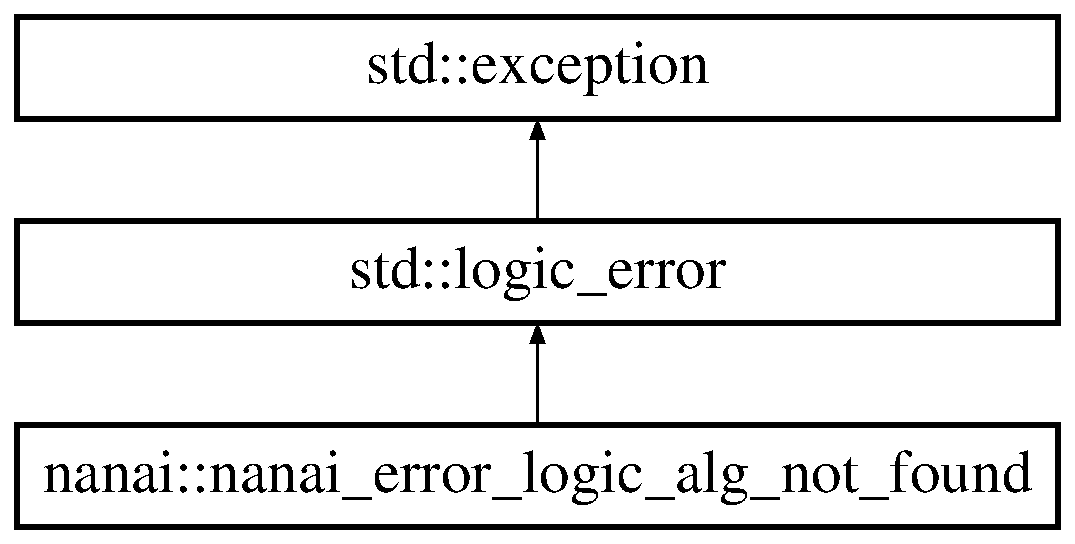
\includegraphics[height=3.000000cm]{classnanai_1_1nanai__error__logic__alg__not__found}
\end{center}
\end{figure}
\subsection*{Public 成员函数}
\begin{DoxyCompactItemize}
\item 
\hyperlink{classnanai_1_1nanai__error__logic__alg__not__found_a37482f1286e3edda3e41e8db08be3899}{nanai\+\_\+error\+\_\+logic\+\_\+alg\+\_\+not\+\_\+found} ()
\end{DoxyCompactItemize}
\subsection*{Public 属性}
\begin{DoxyCompactItemize}
\item 
int \hyperlink{classnanai_1_1nanai__error__logic__alg__not__found_a7701cdbe37605cdaebce0e8a6195e8d9}{\+\_\+errcode}
\end{DoxyCompactItemize}


\subsection{详细描述}


在文件 nanai\+\_\+object.\+h 第 56 行定义.



\subsection{构造及析构函数说明}
\hypertarget{classnanai_1_1nanai__error__logic__alg__not__found_a37482f1286e3edda3e41e8db08be3899}{}\index{nanai\+::nanai\+\_\+error\+\_\+logic\+\_\+alg\+\_\+not\+\_\+found@{nanai\+::nanai\+\_\+error\+\_\+logic\+\_\+alg\+\_\+not\+\_\+found}!nanai\+\_\+error\+\_\+logic\+\_\+alg\+\_\+not\+\_\+found@{nanai\+\_\+error\+\_\+logic\+\_\+alg\+\_\+not\+\_\+found}}
\index{nanai\+\_\+error\+\_\+logic\+\_\+alg\+\_\+not\+\_\+found@{nanai\+\_\+error\+\_\+logic\+\_\+alg\+\_\+not\+\_\+found}!nanai\+::nanai\+\_\+error\+\_\+logic\+\_\+alg\+\_\+not\+\_\+found@{nanai\+::nanai\+\_\+error\+\_\+logic\+\_\+alg\+\_\+not\+\_\+found}}
\subsubsection[{nanai\+\_\+error\+\_\+logic\+\_\+alg\+\_\+not\+\_\+found()}]{\setlength{\rightskip}{0pt plus 5cm}nanai\+::nanai\+\_\+error\+\_\+logic\+\_\+alg\+\_\+not\+\_\+found\+::nanai\+\_\+error\+\_\+logic\+\_\+alg\+\_\+not\+\_\+found (
\begin{DoxyParamCaption}
{}
\end{DoxyParamCaption}
)\hspace{0.3cm}{\ttfamily [explicit]}}\label{classnanai_1_1nanai__error__logic__alg__not__found_a37482f1286e3edda3e41e8db08be3899}


在文件 nanai\+\_\+object.\+cc 第 19 行定义.



\subsection{类成员变量说明}
\hypertarget{classnanai_1_1nanai__error__logic__alg__not__found_a7701cdbe37605cdaebce0e8a6195e8d9}{}\index{nanai\+::nanai\+\_\+error\+\_\+logic\+\_\+alg\+\_\+not\+\_\+found@{nanai\+::nanai\+\_\+error\+\_\+logic\+\_\+alg\+\_\+not\+\_\+found}!\+\_\+errcode@{\+\_\+errcode}}
\index{\+\_\+errcode@{\+\_\+errcode}!nanai\+::nanai\+\_\+error\+\_\+logic\+\_\+alg\+\_\+not\+\_\+found@{nanai\+::nanai\+\_\+error\+\_\+logic\+\_\+alg\+\_\+not\+\_\+found}}
\subsubsection[{\+\_\+errcode}]{\setlength{\rightskip}{0pt plus 5cm}int nanai\+::nanai\+\_\+error\+\_\+logic\+\_\+alg\+\_\+not\+\_\+found\+::\+\_\+errcode}\label{classnanai_1_1nanai__error__logic__alg__not__found_a7701cdbe37605cdaebce0e8a6195e8d9}


在文件 nanai\+\_\+object.\+h 第 60 行定义.



该类的文档由以下文件生成\+:\begin{DoxyCompactItemize}
\item 
inc/\hyperlink{nanai__object_8h}{nanai\+\_\+object.\+h}\item 
src/\hyperlink{nanai__object_8cc}{nanai\+\_\+object.\+cc}\end{DoxyCompactItemize}

\hypertarget{classnanai_1_1nanai__error__logic__home__dir__not__config}{}\section{nanai\+:\+:nanai\+\_\+error\+\_\+logic\+\_\+home\+\_\+dir\+\_\+not\+\_\+config类 参考}
\label{classnanai_1_1nanai__error__logic__home__dir__not__config}\index{nanai\+::nanai\+\_\+error\+\_\+logic\+\_\+home\+\_\+dir\+\_\+not\+\_\+config@{nanai\+::nanai\+\_\+error\+\_\+logic\+\_\+home\+\_\+dir\+\_\+not\+\_\+config}}


{\ttfamily \#include $<$nanai\+\_\+object.\+h$>$}

类 nanai\+:\+:nanai\+\_\+error\+\_\+logic\+\_\+home\+\_\+dir\+\_\+not\+\_\+config 继承关系图\+:\begin{figure}[H]
\begin{center}
\leavevmode
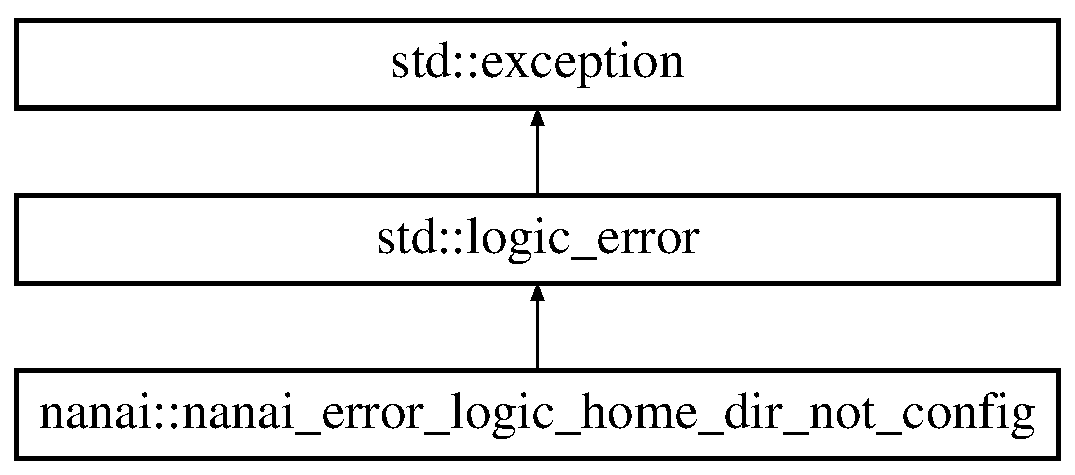
\includegraphics[height=3.000000cm]{classnanai_1_1nanai__error__logic__home__dir__not__config}
\end{center}
\end{figure}
\subsection*{Public 成员函数}
\begin{DoxyCompactItemize}
\item 
\hyperlink{classnanai_1_1nanai__error__logic__home__dir__not__config_a8419fcfc218bb7ec2522eee55fdc6870}{nanai\+\_\+error\+\_\+logic\+\_\+home\+\_\+dir\+\_\+not\+\_\+config} ()
\end{DoxyCompactItemize}
\subsection*{Public 属性}
\begin{DoxyCompactItemize}
\item 
int \hyperlink{classnanai_1_1nanai__error__logic__home__dir__not__config_a9bda795d3a757430411d101bbf9a2df4}{\+\_\+errcode}
\end{DoxyCompactItemize}


\subsection{详细描述}


在文件 nanai\+\_\+object.\+h 第 70 行定义.



\subsection{构造及析构函数说明}
\hypertarget{classnanai_1_1nanai__error__logic__home__dir__not__config_a8419fcfc218bb7ec2522eee55fdc6870}{}\index{nanai\+::nanai\+\_\+error\+\_\+logic\+\_\+home\+\_\+dir\+\_\+not\+\_\+config@{nanai\+::nanai\+\_\+error\+\_\+logic\+\_\+home\+\_\+dir\+\_\+not\+\_\+config}!nanai\+\_\+error\+\_\+logic\+\_\+home\+\_\+dir\+\_\+not\+\_\+config@{nanai\+\_\+error\+\_\+logic\+\_\+home\+\_\+dir\+\_\+not\+\_\+config}}
\index{nanai\+\_\+error\+\_\+logic\+\_\+home\+\_\+dir\+\_\+not\+\_\+config@{nanai\+\_\+error\+\_\+logic\+\_\+home\+\_\+dir\+\_\+not\+\_\+config}!nanai\+::nanai\+\_\+error\+\_\+logic\+\_\+home\+\_\+dir\+\_\+not\+\_\+config@{nanai\+::nanai\+\_\+error\+\_\+logic\+\_\+home\+\_\+dir\+\_\+not\+\_\+config}}
\subsubsection[{nanai\+\_\+error\+\_\+logic\+\_\+home\+\_\+dir\+\_\+not\+\_\+config()}]{\setlength{\rightskip}{0pt plus 5cm}nanai\+::nanai\+\_\+error\+\_\+logic\+\_\+home\+\_\+dir\+\_\+not\+\_\+config\+::nanai\+\_\+error\+\_\+logic\+\_\+home\+\_\+dir\+\_\+not\+\_\+config (
\begin{DoxyParamCaption}
{}
\end{DoxyParamCaption}
)\hspace{0.3cm}{\ttfamily [explicit]}}\label{classnanai_1_1nanai__error__logic__home__dir__not__config_a8419fcfc218bb7ec2522eee55fdc6870}


在文件 nanai\+\_\+object.\+cc 第 27 行定义.



\subsection{类成员变量说明}
\hypertarget{classnanai_1_1nanai__error__logic__home__dir__not__config_a9bda795d3a757430411d101bbf9a2df4}{}\index{nanai\+::nanai\+\_\+error\+\_\+logic\+\_\+home\+\_\+dir\+\_\+not\+\_\+config@{nanai\+::nanai\+\_\+error\+\_\+logic\+\_\+home\+\_\+dir\+\_\+not\+\_\+config}!\+\_\+errcode@{\+\_\+errcode}}
\index{\+\_\+errcode@{\+\_\+errcode}!nanai\+::nanai\+\_\+error\+\_\+logic\+\_\+home\+\_\+dir\+\_\+not\+\_\+config@{nanai\+::nanai\+\_\+error\+\_\+logic\+\_\+home\+\_\+dir\+\_\+not\+\_\+config}}
\subsubsection[{\+\_\+errcode}]{\setlength{\rightskip}{0pt plus 5cm}int nanai\+::nanai\+\_\+error\+\_\+logic\+\_\+home\+\_\+dir\+\_\+not\+\_\+config\+::\+\_\+errcode}\label{classnanai_1_1nanai__error__logic__home__dir__not__config_a9bda795d3a757430411d101bbf9a2df4}


在文件 nanai\+\_\+object.\+h 第 74 行定义.



该类的文档由以下文件生成\+:\begin{DoxyCompactItemize}
\item 
inc/\hyperlink{nanai__object_8h}{nanai\+\_\+object.\+h}\item 
src/\hyperlink{nanai__object_8cc}{nanai\+\_\+object.\+cc}\end{DoxyCompactItemize}

\hypertarget{classnanai_1_1nanai__error__logic__invalid__argument}{}\section{nanai\+:\+:nanai\+\_\+error\+\_\+logic\+\_\+invalid\+\_\+argument类 参考}
\label{classnanai_1_1nanai__error__logic__invalid__argument}\index{nanai\+::nanai\+\_\+error\+\_\+logic\+\_\+invalid\+\_\+argument@{nanai\+::nanai\+\_\+error\+\_\+logic\+\_\+invalid\+\_\+argument}}


{\ttfamily \#include $<$nanai\+\_\+object.\+h$>$}

类 nanai\+:\+:nanai\+\_\+error\+\_\+logic\+\_\+invalid\+\_\+argument 继承关系图\+:\begin{figure}[H]
\begin{center}
\leavevmode
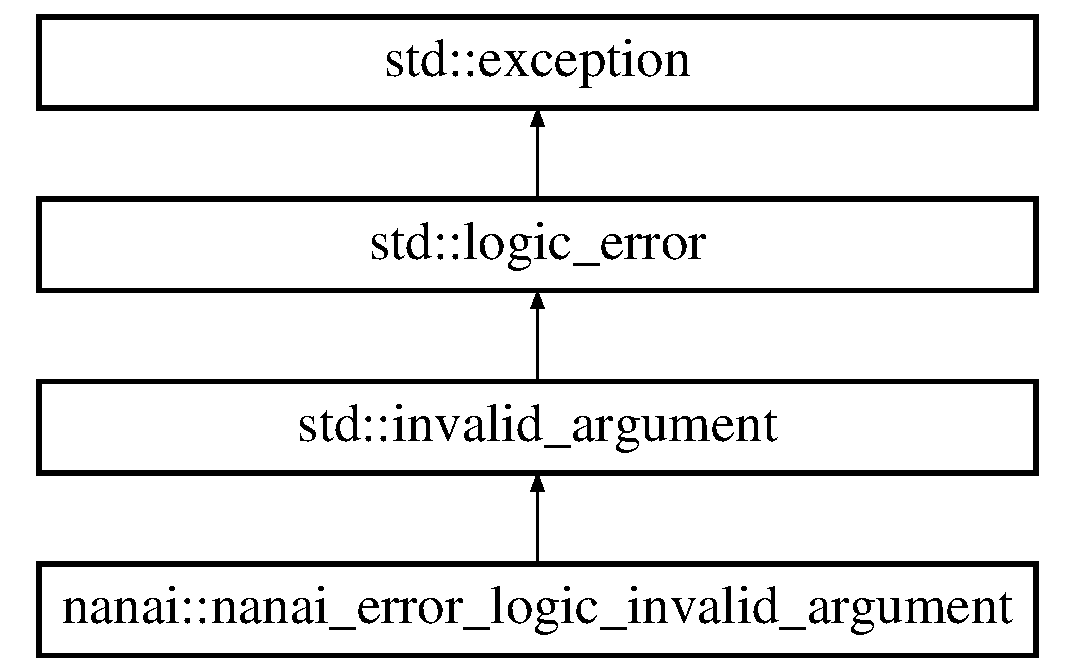
\includegraphics[height=4.000000cm]{classnanai_1_1nanai__error__logic__invalid__argument}
\end{center}
\end{figure}
\subsection*{Public 成员函数}
\begin{DoxyCompactItemize}
\item 
\hyperlink{classnanai_1_1nanai__error__logic__invalid__argument_a4a7a923d0bdaff2a9a450bdfe946adf2}{nanai\+\_\+error\+\_\+logic\+\_\+invalid\+\_\+argument} ()
\end{DoxyCompactItemize}
\subsection*{Public 属性}
\begin{DoxyCompactItemize}
\item 
int \hyperlink{classnanai_1_1nanai__error__logic__invalid__argument_a7a983c95e803de2afbc6220ca65496f4}{\+\_\+errcode}
\end{DoxyCompactItemize}


\subsection{详细描述}


在文件 nanai\+\_\+object.\+h 第 42 行定义.



\subsection{构造及析构函数说明}
\hypertarget{classnanai_1_1nanai__error__logic__invalid__argument_a4a7a923d0bdaff2a9a450bdfe946adf2}{}\index{nanai\+::nanai\+\_\+error\+\_\+logic\+\_\+invalid\+\_\+argument@{nanai\+::nanai\+\_\+error\+\_\+logic\+\_\+invalid\+\_\+argument}!nanai\+\_\+error\+\_\+logic\+\_\+invalid\+\_\+argument@{nanai\+\_\+error\+\_\+logic\+\_\+invalid\+\_\+argument}}
\index{nanai\+\_\+error\+\_\+logic\+\_\+invalid\+\_\+argument@{nanai\+\_\+error\+\_\+logic\+\_\+invalid\+\_\+argument}!nanai\+::nanai\+\_\+error\+\_\+logic\+\_\+invalid\+\_\+argument@{nanai\+::nanai\+\_\+error\+\_\+logic\+\_\+invalid\+\_\+argument}}
\subsubsection[{nanai\+\_\+error\+\_\+logic\+\_\+invalid\+\_\+argument()}]{\setlength{\rightskip}{0pt plus 5cm}nanai\+::nanai\+\_\+error\+\_\+logic\+\_\+invalid\+\_\+argument\+::nanai\+\_\+error\+\_\+logic\+\_\+invalid\+\_\+argument (
\begin{DoxyParamCaption}
{}
\end{DoxyParamCaption}
)\hspace{0.3cm}{\ttfamily [explicit]}}\label{classnanai_1_1nanai__error__logic__invalid__argument_a4a7a923d0bdaff2a9a450bdfe946adf2}


在文件 nanai\+\_\+object.\+cc 第 11 行定义.



\subsection{类成员变量说明}
\hypertarget{classnanai_1_1nanai__error__logic__invalid__argument_a7a983c95e803de2afbc6220ca65496f4}{}\index{nanai\+::nanai\+\_\+error\+\_\+logic\+\_\+invalid\+\_\+argument@{nanai\+::nanai\+\_\+error\+\_\+logic\+\_\+invalid\+\_\+argument}!\+\_\+errcode@{\+\_\+errcode}}
\index{\+\_\+errcode@{\+\_\+errcode}!nanai\+::nanai\+\_\+error\+\_\+logic\+\_\+invalid\+\_\+argument@{nanai\+::nanai\+\_\+error\+\_\+logic\+\_\+invalid\+\_\+argument}}
\subsubsection[{\+\_\+errcode}]{\setlength{\rightskip}{0pt plus 5cm}int nanai\+::nanai\+\_\+error\+\_\+logic\+\_\+invalid\+\_\+argument\+::\+\_\+errcode}\label{classnanai_1_1nanai__error__logic__invalid__argument_a7a983c95e803de2afbc6220ca65496f4}


在文件 nanai\+\_\+object.\+h 第 46 行定义.



该类的文档由以下文件生成\+:\begin{DoxyCompactItemize}
\item 
inc/\hyperlink{nanai__object_8h}{nanai\+\_\+object.\+h}\item 
src/\hyperlink{nanai__object_8cc}{nanai\+\_\+object.\+cc}\end{DoxyCompactItemize}

\hypertarget{classnanai_1_1nanai__error__logic__invalid__config}{}\section{nanai\+:\+:nanai\+\_\+error\+\_\+logic\+\_\+invalid\+\_\+config类 参考}
\label{classnanai_1_1nanai__error__logic__invalid__config}\index{nanai\+::nanai\+\_\+error\+\_\+logic\+\_\+invalid\+\_\+config@{nanai\+::nanai\+\_\+error\+\_\+logic\+\_\+invalid\+\_\+config}}


{\ttfamily \#include $<$nanai\+\_\+object.\+h$>$}

类 nanai\+:\+:nanai\+\_\+error\+\_\+logic\+\_\+invalid\+\_\+config 继承关系图\+:\begin{figure}[H]
\begin{center}
\leavevmode
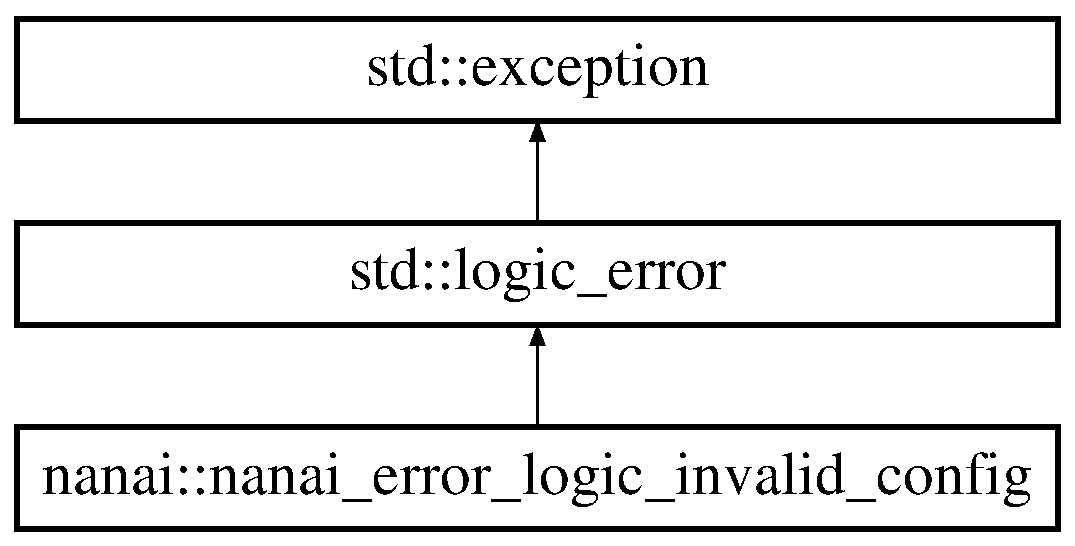
\includegraphics[height=3.000000cm]{classnanai_1_1nanai__error__logic__invalid__config}
\end{center}
\end{figure}
\subsection*{Public 成员函数}
\begin{DoxyCompactItemize}
\item 
\hyperlink{classnanai_1_1nanai__error__logic__invalid__config_a438680feb6cf552fe30c2227286e2a3b}{nanai\+\_\+error\+\_\+logic\+\_\+invalid\+\_\+config} ()
\end{DoxyCompactItemize}
\subsection*{Public 属性}
\begin{DoxyCompactItemize}
\item 
int \hyperlink{classnanai_1_1nanai__error__logic__invalid__config_aaa8c31731609a42d9d3ba8f0def83aa1}{\+\_\+errcode}
\end{DoxyCompactItemize}


\subsection{详细描述}


在文件 nanai\+\_\+object.\+h 第 49 行定义.



\subsection{构造及析构函数说明}
\hypertarget{classnanai_1_1nanai__error__logic__invalid__config_a438680feb6cf552fe30c2227286e2a3b}{}\index{nanai\+::nanai\+\_\+error\+\_\+logic\+\_\+invalid\+\_\+config@{nanai\+::nanai\+\_\+error\+\_\+logic\+\_\+invalid\+\_\+config}!nanai\+\_\+error\+\_\+logic\+\_\+invalid\+\_\+config@{nanai\+\_\+error\+\_\+logic\+\_\+invalid\+\_\+config}}
\index{nanai\+\_\+error\+\_\+logic\+\_\+invalid\+\_\+config@{nanai\+\_\+error\+\_\+logic\+\_\+invalid\+\_\+config}!nanai\+::nanai\+\_\+error\+\_\+logic\+\_\+invalid\+\_\+config@{nanai\+::nanai\+\_\+error\+\_\+logic\+\_\+invalid\+\_\+config}}
\subsubsection[{nanai\+\_\+error\+\_\+logic\+\_\+invalid\+\_\+config()}]{\setlength{\rightskip}{0pt plus 5cm}nanai\+::nanai\+\_\+error\+\_\+logic\+\_\+invalid\+\_\+config\+::nanai\+\_\+error\+\_\+logic\+\_\+invalid\+\_\+config (
\begin{DoxyParamCaption}
{}
\end{DoxyParamCaption}
)\hspace{0.3cm}{\ttfamily [explicit]}}\label{classnanai_1_1nanai__error__logic__invalid__config_a438680feb6cf552fe30c2227286e2a3b}


在文件 nanai\+\_\+object.\+cc 第 15 行定义.



\subsection{类成员变量说明}
\hypertarget{classnanai_1_1nanai__error__logic__invalid__config_aaa8c31731609a42d9d3ba8f0def83aa1}{}\index{nanai\+::nanai\+\_\+error\+\_\+logic\+\_\+invalid\+\_\+config@{nanai\+::nanai\+\_\+error\+\_\+logic\+\_\+invalid\+\_\+config}!\+\_\+errcode@{\+\_\+errcode}}
\index{\+\_\+errcode@{\+\_\+errcode}!nanai\+::nanai\+\_\+error\+\_\+logic\+\_\+invalid\+\_\+config@{nanai\+::nanai\+\_\+error\+\_\+logic\+\_\+invalid\+\_\+config}}
\subsubsection[{\+\_\+errcode}]{\setlength{\rightskip}{0pt plus 5cm}int nanai\+::nanai\+\_\+error\+\_\+logic\+\_\+invalid\+\_\+config\+::\+\_\+errcode}\label{classnanai_1_1nanai__error__logic__invalid__config_aaa8c31731609a42d9d3ba8f0def83aa1}


在文件 nanai\+\_\+object.\+h 第 53 行定义.



该类的文档由以下文件生成\+:\begin{DoxyCompactItemize}
\item 
inc/\hyperlink{nanai__object_8h}{nanai\+\_\+object.\+h}\item 
src/\hyperlink{nanai__object_8cc}{nanai\+\_\+object.\+cc}\end{DoxyCompactItemize}

\hypertarget{classnanai_1_1nanai__error__logic__task__not__matched}{}\section{nanai\+:\+:nanai\+\_\+error\+\_\+logic\+\_\+task\+\_\+not\+\_\+matched类 参考}
\label{classnanai_1_1nanai__error__logic__task__not__matched}\index{nanai\+::nanai\+\_\+error\+\_\+logic\+\_\+task\+\_\+not\+\_\+matched@{nanai\+::nanai\+\_\+error\+\_\+logic\+\_\+task\+\_\+not\+\_\+matched}}


{\ttfamily \#include $<$nanai\+\_\+object.\+h$>$}

类 nanai\+:\+:nanai\+\_\+error\+\_\+logic\+\_\+task\+\_\+not\+\_\+matched 继承关系图\+:\begin{figure}[H]
\begin{center}
\leavevmode
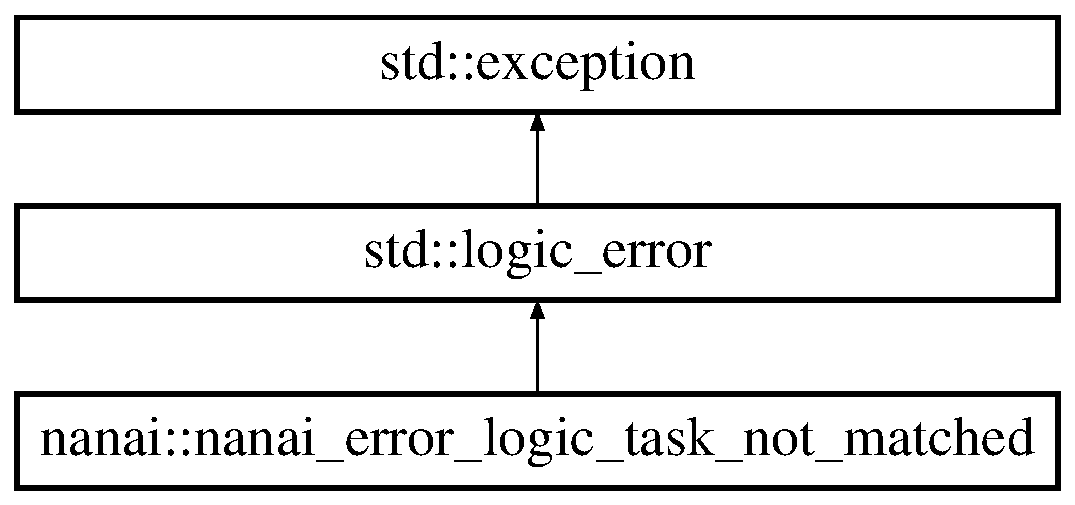
\includegraphics[height=3.000000cm]{classnanai_1_1nanai__error__logic__task__not__matched}
\end{center}
\end{figure}
\subsection*{Public 成员函数}
\begin{DoxyCompactItemize}
\item 
\hyperlink{classnanai_1_1nanai__error__logic__task__not__matched_a94f76745dd25d220afd5dea030f07496}{nanai\+\_\+error\+\_\+logic\+\_\+task\+\_\+not\+\_\+matched} ()
\end{DoxyCompactItemize}
\subsection*{Public 属性}
\begin{DoxyCompactItemize}
\item 
int \hyperlink{classnanai_1_1nanai__error__logic__task__not__matched_a3e73ce12d629068c63360384585d62c9}{\+\_\+errcode}
\end{DoxyCompactItemize}


\subsection{详细描述}


在文件 nanai\+\_\+object.\+h 第 64 行定义.



\subsection{构造及析构函数说明}
\hypertarget{classnanai_1_1nanai__error__logic__task__not__matched_a94f76745dd25d220afd5dea030f07496}{}\index{nanai\+::nanai\+\_\+error\+\_\+logic\+\_\+task\+\_\+not\+\_\+matched@{nanai\+::nanai\+\_\+error\+\_\+logic\+\_\+task\+\_\+not\+\_\+matched}!nanai\+\_\+error\+\_\+logic\+\_\+task\+\_\+not\+\_\+matched@{nanai\+\_\+error\+\_\+logic\+\_\+task\+\_\+not\+\_\+matched}}
\index{nanai\+\_\+error\+\_\+logic\+\_\+task\+\_\+not\+\_\+matched@{nanai\+\_\+error\+\_\+logic\+\_\+task\+\_\+not\+\_\+matched}!nanai\+::nanai\+\_\+error\+\_\+logic\+\_\+task\+\_\+not\+\_\+matched@{nanai\+::nanai\+\_\+error\+\_\+logic\+\_\+task\+\_\+not\+\_\+matched}}
\subsubsection[{nanai\+\_\+error\+\_\+logic\+\_\+task\+\_\+not\+\_\+matched()}]{\setlength{\rightskip}{0pt plus 5cm}nanai\+::nanai\+\_\+error\+\_\+logic\+\_\+task\+\_\+not\+\_\+matched\+::nanai\+\_\+error\+\_\+logic\+\_\+task\+\_\+not\+\_\+matched (
\begin{DoxyParamCaption}
{}
\end{DoxyParamCaption}
)\hspace{0.3cm}{\ttfamily [explicit]}}\label{classnanai_1_1nanai__error__logic__task__not__matched_a94f76745dd25d220afd5dea030f07496}


在文件 nanai\+\_\+object.\+cc 第 23 行定义.



\subsection{类成员变量说明}
\hypertarget{classnanai_1_1nanai__error__logic__task__not__matched_a3e73ce12d629068c63360384585d62c9}{}\index{nanai\+::nanai\+\_\+error\+\_\+logic\+\_\+task\+\_\+not\+\_\+matched@{nanai\+::nanai\+\_\+error\+\_\+logic\+\_\+task\+\_\+not\+\_\+matched}!\+\_\+errcode@{\+\_\+errcode}}
\index{\+\_\+errcode@{\+\_\+errcode}!nanai\+::nanai\+\_\+error\+\_\+logic\+\_\+task\+\_\+not\+\_\+matched@{nanai\+::nanai\+\_\+error\+\_\+logic\+\_\+task\+\_\+not\+\_\+matched}}
\subsubsection[{\+\_\+errcode}]{\setlength{\rightskip}{0pt plus 5cm}int nanai\+::nanai\+\_\+error\+\_\+logic\+\_\+task\+\_\+not\+\_\+matched\+::\+\_\+errcode}\label{classnanai_1_1nanai__error__logic__task__not__matched_a3e73ce12d629068c63360384585d62c9}


在文件 nanai\+\_\+object.\+h 第 68 行定义.



该类的文档由以下文件生成\+:\begin{DoxyCompactItemize}
\item 
inc/\hyperlink{nanai__object_8h}{nanai\+\_\+object.\+h}\item 
src/\hyperlink{nanai__object_8cc}{nanai\+\_\+object.\+cc}\end{DoxyCompactItemize}

\hypertarget{classnanai_1_1nanai__error__runtime__alloc__memory}{}\section{nanai\+:\+:nanai\+\_\+error\+\_\+runtime\+\_\+alloc\+\_\+memory类 参考}
\label{classnanai_1_1nanai__error__runtime__alloc__memory}\index{nanai\+::nanai\+\_\+error\+\_\+runtime\+\_\+alloc\+\_\+memory@{nanai\+::nanai\+\_\+error\+\_\+runtime\+\_\+alloc\+\_\+memory}}


{\ttfamily \#include $<$nanai\+\_\+object.\+h$>$}

类 nanai\+:\+:nanai\+\_\+error\+\_\+runtime\+\_\+alloc\+\_\+memory 继承关系图\+:\begin{figure}[H]
\begin{center}
\leavevmode
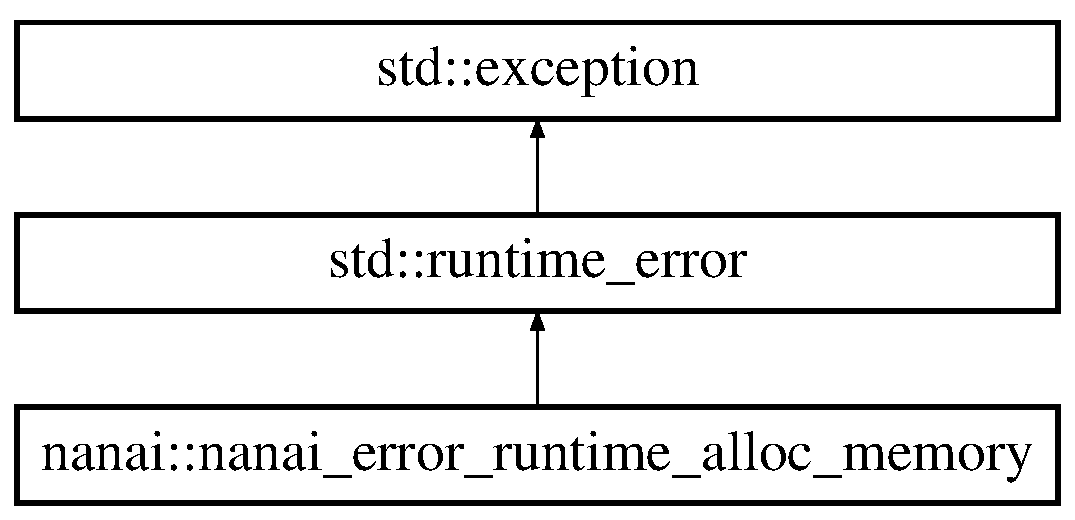
\includegraphics[height=3.000000cm]{classnanai_1_1nanai__error__runtime__alloc__memory}
\end{center}
\end{figure}
\subsection*{Public 成员函数}
\begin{DoxyCompactItemize}
\item 
\hyperlink{classnanai_1_1nanai__error__runtime__alloc__memory_aa638631a5e632fc47409027525c58401}{nanai\+\_\+error\+\_\+runtime\+\_\+alloc\+\_\+memory} ()
\end{DoxyCompactItemize}
\subsection*{Public 属性}
\begin{DoxyCompactItemize}
\item 
int \hyperlink{classnanai_1_1nanai__error__runtime__alloc__memory_a3212283dfac6316bc3ac8e3c2f7578df}{\+\_\+errcode}
\end{DoxyCompactItemize}


\subsection{详细描述}


在文件 nanai\+\_\+object.\+h 第 134 行定义.



\subsection{构造及析构函数说明}
\hypertarget{classnanai_1_1nanai__error__runtime__alloc__memory_aa638631a5e632fc47409027525c58401}{}\index{nanai\+::nanai\+\_\+error\+\_\+runtime\+\_\+alloc\+\_\+memory@{nanai\+::nanai\+\_\+error\+\_\+runtime\+\_\+alloc\+\_\+memory}!nanai\+\_\+error\+\_\+runtime\+\_\+alloc\+\_\+memory@{nanai\+\_\+error\+\_\+runtime\+\_\+alloc\+\_\+memory}}
\index{nanai\+\_\+error\+\_\+runtime\+\_\+alloc\+\_\+memory@{nanai\+\_\+error\+\_\+runtime\+\_\+alloc\+\_\+memory}!nanai\+::nanai\+\_\+error\+\_\+runtime\+\_\+alloc\+\_\+memory@{nanai\+::nanai\+\_\+error\+\_\+runtime\+\_\+alloc\+\_\+memory}}
\subsubsection[{nanai\+\_\+error\+\_\+runtime\+\_\+alloc\+\_\+memory()}]{\setlength{\rightskip}{0pt plus 5cm}nanai\+::nanai\+\_\+error\+\_\+runtime\+\_\+alloc\+\_\+memory\+::nanai\+\_\+error\+\_\+runtime\+\_\+alloc\+\_\+memory (
\begin{DoxyParamCaption}
{}
\end{DoxyParamCaption}
)\hspace{0.3cm}{\ttfamily [explicit]}}\label{classnanai_1_1nanai__error__runtime__alloc__memory_aa638631a5e632fc47409027525c58401}


在文件 nanai\+\_\+object.\+cc 第 63 行定义.



\subsection{类成员变量说明}
\hypertarget{classnanai_1_1nanai__error__runtime__alloc__memory_a3212283dfac6316bc3ac8e3c2f7578df}{}\index{nanai\+::nanai\+\_\+error\+\_\+runtime\+\_\+alloc\+\_\+memory@{nanai\+::nanai\+\_\+error\+\_\+runtime\+\_\+alloc\+\_\+memory}!\+\_\+errcode@{\+\_\+errcode}}
\index{\+\_\+errcode@{\+\_\+errcode}!nanai\+::nanai\+\_\+error\+\_\+runtime\+\_\+alloc\+\_\+memory@{nanai\+::nanai\+\_\+error\+\_\+runtime\+\_\+alloc\+\_\+memory}}
\subsubsection[{\+\_\+errcode}]{\setlength{\rightskip}{0pt plus 5cm}int nanai\+::nanai\+\_\+error\+\_\+runtime\+\_\+alloc\+\_\+memory\+::\+\_\+errcode}\label{classnanai_1_1nanai__error__runtime__alloc__memory_a3212283dfac6316bc3ac8e3c2f7578df}


在文件 nanai\+\_\+object.\+h 第 138 行定义.



该类的文档由以下文件生成\+:\begin{DoxyCompactItemize}
\item 
inc/\hyperlink{nanai__object_8h}{nanai\+\_\+object.\+h}\item 
src/\hyperlink{nanai__object_8cc}{nanai\+\_\+object.\+cc}\end{DoxyCompactItemize}

\hypertarget{classnanai_1_1nanai__error__runtime__create__thread}{}\section{nanai\+:\+:nanai\+\_\+error\+\_\+runtime\+\_\+create\+\_\+thread类 参考}
\label{classnanai_1_1nanai__error__runtime__create__thread}\index{nanai\+::nanai\+\_\+error\+\_\+runtime\+\_\+create\+\_\+thread@{nanai\+::nanai\+\_\+error\+\_\+runtime\+\_\+create\+\_\+thread}}


{\ttfamily \#include $<$nanai\+\_\+object.\+h$>$}

类 nanai\+:\+:nanai\+\_\+error\+\_\+runtime\+\_\+create\+\_\+thread 继承关系图\+:\begin{figure}[H]
\begin{center}
\leavevmode
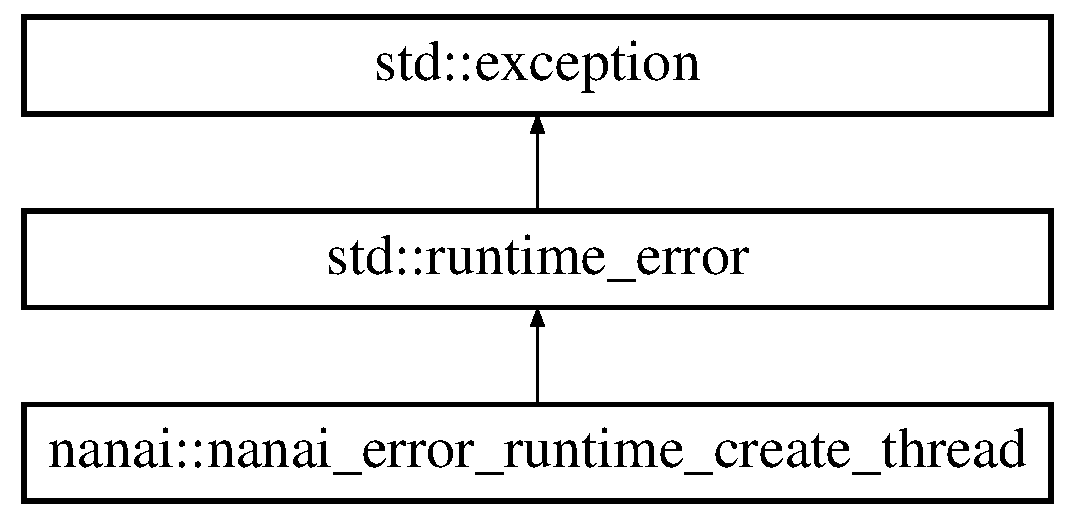
\includegraphics[height=3.000000cm]{classnanai_1_1nanai__error__runtime__create__thread}
\end{center}
\end{figure}
\subsection*{Public 成员函数}
\begin{DoxyCompactItemize}
\item 
\hyperlink{classnanai_1_1nanai__error__runtime__create__thread_aace42682861730c6af0a207b76b3c329}{nanai\+\_\+error\+\_\+runtime\+\_\+create\+\_\+thread} ()
\end{DoxyCompactItemize}
\subsection*{Public 属性}
\begin{DoxyCompactItemize}
\item 
int \hyperlink{classnanai_1_1nanai__error__runtime__create__thread_abc60a585972bae43ec4d6801097bb5ba}{\+\_\+errcode}
\end{DoxyCompactItemize}


\subsection{详细描述}


在文件 nanai\+\_\+object.\+h 第 85 行定义.



\subsection{构造及析构函数说明}
\hypertarget{classnanai_1_1nanai__error__runtime__create__thread_aace42682861730c6af0a207b76b3c329}{}\index{nanai\+::nanai\+\_\+error\+\_\+runtime\+\_\+create\+\_\+thread@{nanai\+::nanai\+\_\+error\+\_\+runtime\+\_\+create\+\_\+thread}!nanai\+\_\+error\+\_\+runtime\+\_\+create\+\_\+thread@{nanai\+\_\+error\+\_\+runtime\+\_\+create\+\_\+thread}}
\index{nanai\+\_\+error\+\_\+runtime\+\_\+create\+\_\+thread@{nanai\+\_\+error\+\_\+runtime\+\_\+create\+\_\+thread}!nanai\+::nanai\+\_\+error\+\_\+runtime\+\_\+create\+\_\+thread@{nanai\+::nanai\+\_\+error\+\_\+runtime\+\_\+create\+\_\+thread}}
\subsubsection[{nanai\+\_\+error\+\_\+runtime\+\_\+create\+\_\+thread()}]{\setlength{\rightskip}{0pt plus 5cm}nanai\+::nanai\+\_\+error\+\_\+runtime\+\_\+create\+\_\+thread\+::nanai\+\_\+error\+\_\+runtime\+\_\+create\+\_\+thread (
\begin{DoxyParamCaption}
{}
\end{DoxyParamCaption}
)\hspace{0.3cm}{\ttfamily [explicit]}}\label{classnanai_1_1nanai__error__runtime__create__thread_aace42682861730c6af0a207b76b3c329}


在文件 nanai\+\_\+object.\+cc 第 35 行定义.



\subsection{类成员变量说明}
\hypertarget{classnanai_1_1nanai__error__runtime__create__thread_abc60a585972bae43ec4d6801097bb5ba}{}\index{nanai\+::nanai\+\_\+error\+\_\+runtime\+\_\+create\+\_\+thread@{nanai\+::nanai\+\_\+error\+\_\+runtime\+\_\+create\+\_\+thread}!\+\_\+errcode@{\+\_\+errcode}}
\index{\+\_\+errcode@{\+\_\+errcode}!nanai\+::nanai\+\_\+error\+\_\+runtime\+\_\+create\+\_\+thread@{nanai\+::nanai\+\_\+error\+\_\+runtime\+\_\+create\+\_\+thread}}
\subsubsection[{\+\_\+errcode}]{\setlength{\rightskip}{0pt plus 5cm}int nanai\+::nanai\+\_\+error\+\_\+runtime\+\_\+create\+\_\+thread\+::\+\_\+errcode}\label{classnanai_1_1nanai__error__runtime__create__thread_abc60a585972bae43ec4d6801097bb5ba}


在文件 nanai\+\_\+object.\+h 第 89 行定义.



该类的文档由以下文件生成\+:\begin{DoxyCompactItemize}
\item 
inc/\hyperlink{nanai__object_8h}{nanai\+\_\+object.\+h}\item 
src/\hyperlink{nanai__object_8cc}{nanai\+\_\+object.\+cc}\end{DoxyCompactItemize}

\hypertarget{classnanai_1_1nanai__error__runtime__destroy__mutex}{}\section{nanai\+:\+:nanai\+\_\+error\+\_\+runtime\+\_\+destroy\+\_\+mutex类 参考}
\label{classnanai_1_1nanai__error__runtime__destroy__mutex}\index{nanai\+::nanai\+\_\+error\+\_\+runtime\+\_\+destroy\+\_\+mutex@{nanai\+::nanai\+\_\+error\+\_\+runtime\+\_\+destroy\+\_\+mutex}}


{\ttfamily \#include $<$nanai\+\_\+object.\+h$>$}

类 nanai\+:\+:nanai\+\_\+error\+\_\+runtime\+\_\+destroy\+\_\+mutex 继承关系图\+:\begin{figure}[H]
\begin{center}
\leavevmode
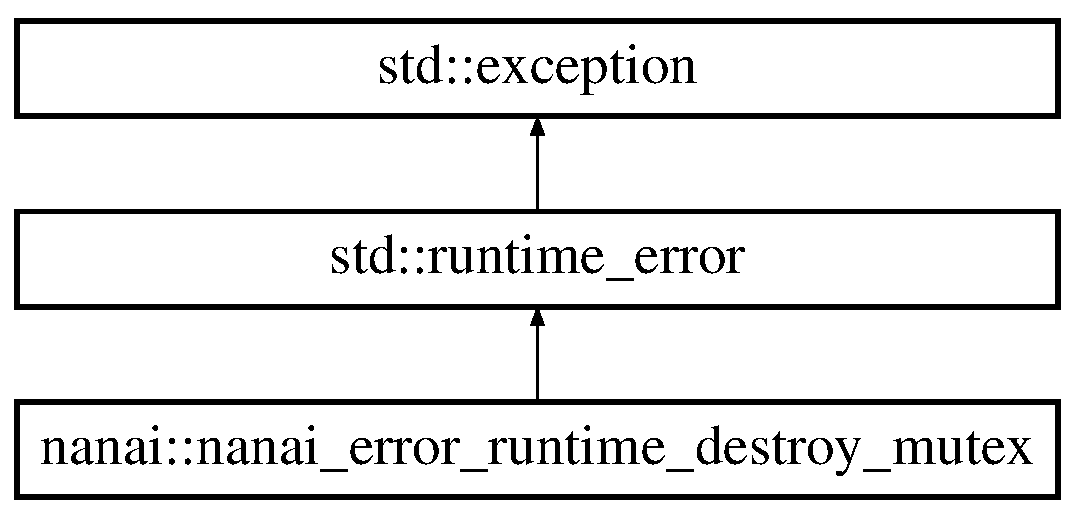
\includegraphics[height=3.000000cm]{classnanai_1_1nanai__error__runtime__destroy__mutex}
\end{center}
\end{figure}
\subsection*{Public 成员函数}
\begin{DoxyCompactItemize}
\item 
\hyperlink{classnanai_1_1nanai__error__runtime__destroy__mutex_a8cf012bdc03827ba61f3d3825c9c3ee4}{nanai\+\_\+error\+\_\+runtime\+\_\+destroy\+\_\+mutex} ()
\end{DoxyCompactItemize}
\subsection*{Public 属性}
\begin{DoxyCompactItemize}
\item 
int \hyperlink{classnanai_1_1nanai__error__runtime__destroy__mutex_a8d75df933f0f165a5d9ee57173c3dd21}{\+\_\+errcode}
\end{DoxyCompactItemize}


\subsection{详细描述}


在文件 nanai\+\_\+object.\+h 第 99 行定义.



\subsection{构造及析构函数说明}
\hypertarget{classnanai_1_1nanai__error__runtime__destroy__mutex_a8cf012bdc03827ba61f3d3825c9c3ee4}{}\index{nanai\+::nanai\+\_\+error\+\_\+runtime\+\_\+destroy\+\_\+mutex@{nanai\+::nanai\+\_\+error\+\_\+runtime\+\_\+destroy\+\_\+mutex}!nanai\+\_\+error\+\_\+runtime\+\_\+destroy\+\_\+mutex@{nanai\+\_\+error\+\_\+runtime\+\_\+destroy\+\_\+mutex}}
\index{nanai\+\_\+error\+\_\+runtime\+\_\+destroy\+\_\+mutex@{nanai\+\_\+error\+\_\+runtime\+\_\+destroy\+\_\+mutex}!nanai\+::nanai\+\_\+error\+\_\+runtime\+\_\+destroy\+\_\+mutex@{nanai\+::nanai\+\_\+error\+\_\+runtime\+\_\+destroy\+\_\+mutex}}
\subsubsection[{nanai\+\_\+error\+\_\+runtime\+\_\+destroy\+\_\+mutex()}]{\setlength{\rightskip}{0pt plus 5cm}nanai\+::nanai\+\_\+error\+\_\+runtime\+\_\+destroy\+\_\+mutex\+::nanai\+\_\+error\+\_\+runtime\+\_\+destroy\+\_\+mutex (
\begin{DoxyParamCaption}
{}
\end{DoxyParamCaption}
)\hspace{0.3cm}{\ttfamily [explicit]}}\label{classnanai_1_1nanai__error__runtime__destroy__mutex_a8cf012bdc03827ba61f3d3825c9c3ee4}


在文件 nanai\+\_\+object.\+cc 第 43 行定义.



\subsection{类成员变量说明}
\hypertarget{classnanai_1_1nanai__error__runtime__destroy__mutex_a8d75df933f0f165a5d9ee57173c3dd21}{}\index{nanai\+::nanai\+\_\+error\+\_\+runtime\+\_\+destroy\+\_\+mutex@{nanai\+::nanai\+\_\+error\+\_\+runtime\+\_\+destroy\+\_\+mutex}!\+\_\+errcode@{\+\_\+errcode}}
\index{\+\_\+errcode@{\+\_\+errcode}!nanai\+::nanai\+\_\+error\+\_\+runtime\+\_\+destroy\+\_\+mutex@{nanai\+::nanai\+\_\+error\+\_\+runtime\+\_\+destroy\+\_\+mutex}}
\subsubsection[{\+\_\+errcode}]{\setlength{\rightskip}{0pt plus 5cm}int nanai\+::nanai\+\_\+error\+\_\+runtime\+\_\+destroy\+\_\+mutex\+::\+\_\+errcode}\label{classnanai_1_1nanai__error__runtime__destroy__mutex_a8d75df933f0f165a5d9ee57173c3dd21}


在文件 nanai\+\_\+object.\+h 第 103 行定义.



该类的文档由以下文件生成\+:\begin{DoxyCompactItemize}
\item 
inc/\hyperlink{nanai__object_8h}{nanai\+\_\+object.\+h}\item 
src/\hyperlink{nanai__object_8cc}{nanai\+\_\+object.\+cc}\end{DoxyCompactItemize}

\hypertarget{classnanai_1_1nanai__error__runtime__init__mutex}{}\section{nanai\+:\+:nanai\+\_\+error\+\_\+runtime\+\_\+init\+\_\+mutex类 参考}
\label{classnanai_1_1nanai__error__runtime__init__mutex}\index{nanai\+::nanai\+\_\+error\+\_\+runtime\+\_\+init\+\_\+mutex@{nanai\+::nanai\+\_\+error\+\_\+runtime\+\_\+init\+\_\+mutex}}


{\ttfamily \#include $<$nanai\+\_\+object.\+h$>$}

类 nanai\+:\+:nanai\+\_\+error\+\_\+runtime\+\_\+init\+\_\+mutex 继承关系图\+:\begin{figure}[H]
\begin{center}
\leavevmode
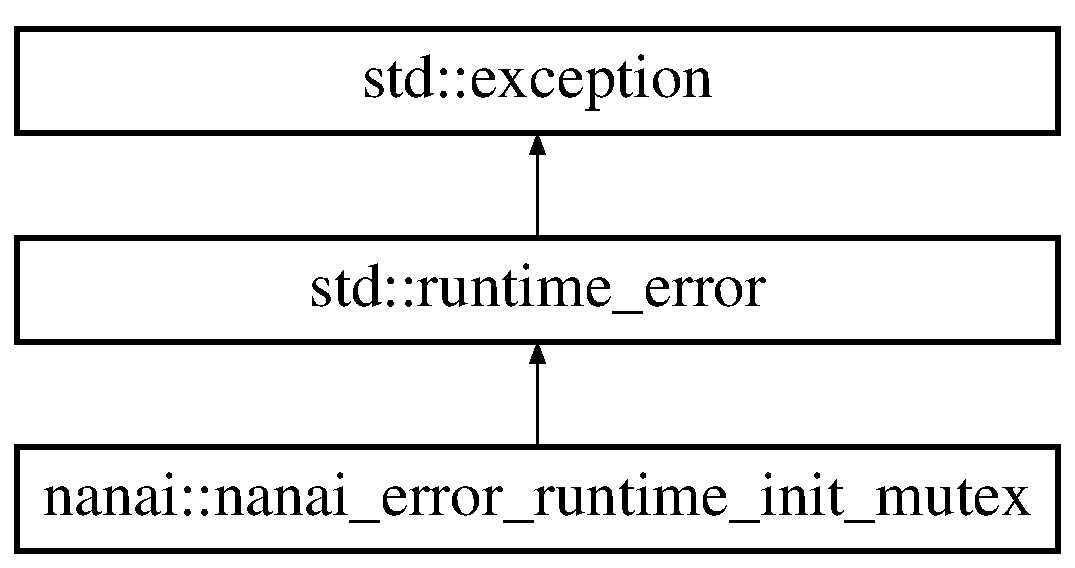
\includegraphics[height=3.000000cm]{classnanai_1_1nanai__error__runtime__init__mutex}
\end{center}
\end{figure}
\subsection*{Public 成员函数}
\begin{DoxyCompactItemize}
\item 
\hyperlink{classnanai_1_1nanai__error__runtime__init__mutex_a0013394fd311166a8407be53eba690a6}{nanai\+\_\+error\+\_\+runtime\+\_\+init\+\_\+mutex} ()
\end{DoxyCompactItemize}
\subsection*{Public 属性}
\begin{DoxyCompactItemize}
\item 
int \hyperlink{classnanai_1_1nanai__error__runtime__init__mutex_a9cf39ee56a510b20711a828030b72c96}{\+\_\+errcode}
\end{DoxyCompactItemize}


\subsection{详细描述}


在文件 nanai\+\_\+object.\+h 第 84 行定义.



\subsection{构造及析构函数说明}
\hypertarget{classnanai_1_1nanai__error__runtime__init__mutex_a0013394fd311166a8407be53eba690a6}{}\index{nanai\+::nanai\+\_\+error\+\_\+runtime\+\_\+init\+\_\+mutex@{nanai\+::nanai\+\_\+error\+\_\+runtime\+\_\+init\+\_\+mutex}!nanai\+\_\+error\+\_\+runtime\+\_\+init\+\_\+mutex@{nanai\+\_\+error\+\_\+runtime\+\_\+init\+\_\+mutex}}
\index{nanai\+\_\+error\+\_\+runtime\+\_\+init\+\_\+mutex@{nanai\+\_\+error\+\_\+runtime\+\_\+init\+\_\+mutex}!nanai\+::nanai\+\_\+error\+\_\+runtime\+\_\+init\+\_\+mutex@{nanai\+::nanai\+\_\+error\+\_\+runtime\+\_\+init\+\_\+mutex}}
\subsubsection[{nanai\+\_\+error\+\_\+runtime\+\_\+init\+\_\+mutex()}]{\setlength{\rightskip}{0pt plus 5cm}nanai\+::nanai\+\_\+error\+\_\+runtime\+\_\+init\+\_\+mutex\+::nanai\+\_\+error\+\_\+runtime\+\_\+init\+\_\+mutex (
\begin{DoxyParamCaption}
{}
\end{DoxyParamCaption}
)\hspace{0.3cm}{\ttfamily [explicit]}}\label{classnanai_1_1nanai__error__runtime__init__mutex_a0013394fd311166a8407be53eba690a6}


在文件 nanai\+\_\+object.\+cc 第 35 行定义.



\subsection{类成员变量说明}
\hypertarget{classnanai_1_1nanai__error__runtime__init__mutex_a9cf39ee56a510b20711a828030b72c96}{}\index{nanai\+::nanai\+\_\+error\+\_\+runtime\+\_\+init\+\_\+mutex@{nanai\+::nanai\+\_\+error\+\_\+runtime\+\_\+init\+\_\+mutex}!\+\_\+errcode@{\+\_\+errcode}}
\index{\+\_\+errcode@{\+\_\+errcode}!nanai\+::nanai\+\_\+error\+\_\+runtime\+\_\+init\+\_\+mutex@{nanai\+::nanai\+\_\+error\+\_\+runtime\+\_\+init\+\_\+mutex}}
\subsubsection[{\+\_\+errcode}]{\setlength{\rightskip}{0pt plus 5cm}int nanai\+::nanai\+\_\+error\+\_\+runtime\+\_\+init\+\_\+mutex\+::\+\_\+errcode}\label{classnanai_1_1nanai__error__runtime__init__mutex_a9cf39ee56a510b20711a828030b72c96}


在文件 nanai\+\_\+object.\+h 第 88 行定义.



该类的文档由以下文件生成\+:\begin{DoxyCompactItemize}
\item 
inc/\hyperlink{nanai__object_8h}{nanai\+\_\+object.\+h}\item 
src/\hyperlink{nanai__object_8cc}{nanai\+\_\+object.\+cc}\end{DoxyCompactItemize}

\hypertarget{classnanai_1_1nanai__error__runtime__join__thread}{}\section{nanai\+:\+:nanai\+\_\+error\+\_\+runtime\+\_\+join\+\_\+thread类 参考}
\label{classnanai_1_1nanai__error__runtime__join__thread}\index{nanai\+::nanai\+\_\+error\+\_\+runtime\+\_\+join\+\_\+thread@{nanai\+::nanai\+\_\+error\+\_\+runtime\+\_\+join\+\_\+thread}}


{\ttfamily \#include $<$nanai\+\_\+object.\+h$>$}

类 nanai\+:\+:nanai\+\_\+error\+\_\+runtime\+\_\+join\+\_\+thread 继承关系图\+:\begin{figure}[H]
\begin{center}
\leavevmode
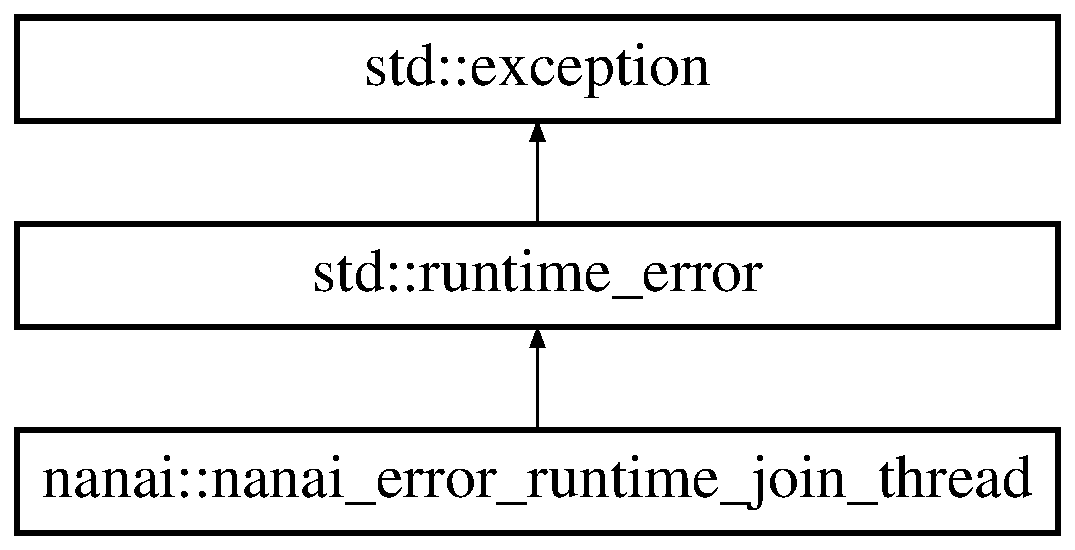
\includegraphics[height=3.000000cm]{classnanai_1_1nanai__error__runtime__join__thread}
\end{center}
\end{figure}
\subsection*{Public 成员函数}
\begin{DoxyCompactItemize}
\item 
\hyperlink{classnanai_1_1nanai__error__runtime__join__thread_aa6319913367e8964e54866f35c763435}{nanai\+\_\+error\+\_\+runtime\+\_\+join\+\_\+thread} ()
\end{DoxyCompactItemize}
\subsection*{Public 属性}
\begin{DoxyCompactItemize}
\item 
int \hyperlink{classnanai_1_1nanai__error__runtime__join__thread_ad213745f7db3d98b873fb826187ed642}{\+\_\+errcode}
\end{DoxyCompactItemize}


\subsection{详细描述}


在文件 nanai\+\_\+object.\+h 第 112 行定义.



\subsection{构造及析构函数说明}
\hypertarget{classnanai_1_1nanai__error__runtime__join__thread_aa6319913367e8964e54866f35c763435}{}\index{nanai\+::nanai\+\_\+error\+\_\+runtime\+\_\+join\+\_\+thread@{nanai\+::nanai\+\_\+error\+\_\+runtime\+\_\+join\+\_\+thread}!nanai\+\_\+error\+\_\+runtime\+\_\+join\+\_\+thread@{nanai\+\_\+error\+\_\+runtime\+\_\+join\+\_\+thread}}
\index{nanai\+\_\+error\+\_\+runtime\+\_\+join\+\_\+thread@{nanai\+\_\+error\+\_\+runtime\+\_\+join\+\_\+thread}!nanai\+::nanai\+\_\+error\+\_\+runtime\+\_\+join\+\_\+thread@{nanai\+::nanai\+\_\+error\+\_\+runtime\+\_\+join\+\_\+thread}}
\subsubsection[{nanai\+\_\+error\+\_\+runtime\+\_\+join\+\_\+thread()}]{\setlength{\rightskip}{0pt plus 5cm}nanai\+::nanai\+\_\+error\+\_\+runtime\+\_\+join\+\_\+thread\+::nanai\+\_\+error\+\_\+runtime\+\_\+join\+\_\+thread (
\begin{DoxyParamCaption}
{}
\end{DoxyParamCaption}
)\hspace{0.3cm}{\ttfamily [explicit]}}\label{classnanai_1_1nanai__error__runtime__join__thread_aa6319913367e8964e54866f35c763435}


在文件 nanai\+\_\+object.\+cc 第 51 行定义.



\subsection{类成员变量说明}
\hypertarget{classnanai_1_1nanai__error__runtime__join__thread_ad213745f7db3d98b873fb826187ed642}{}\index{nanai\+::nanai\+\_\+error\+\_\+runtime\+\_\+join\+\_\+thread@{nanai\+::nanai\+\_\+error\+\_\+runtime\+\_\+join\+\_\+thread}!\+\_\+errcode@{\+\_\+errcode}}
\index{\+\_\+errcode@{\+\_\+errcode}!nanai\+::nanai\+\_\+error\+\_\+runtime\+\_\+join\+\_\+thread@{nanai\+::nanai\+\_\+error\+\_\+runtime\+\_\+join\+\_\+thread}}
\subsubsection[{\+\_\+errcode}]{\setlength{\rightskip}{0pt plus 5cm}int nanai\+::nanai\+\_\+error\+\_\+runtime\+\_\+join\+\_\+thread\+::\+\_\+errcode}\label{classnanai_1_1nanai__error__runtime__join__thread_ad213745f7db3d98b873fb826187ed642}


在文件 nanai\+\_\+object.\+h 第 116 行定义.



该类的文档由以下文件生成\+:\begin{DoxyCompactItemize}
\item 
inc/\hyperlink{nanai__object_8h}{nanai\+\_\+object.\+h}\item 
src/\hyperlink{nanai__object_8cc}{nanai\+\_\+object.\+cc}\end{DoxyCompactItemize}

\hypertarget{classnanai_1_1nanai__error__runtime__lock__mutex}{}\section{nanai\+:\+:nanai\+\_\+error\+\_\+runtime\+\_\+lock\+\_\+mutex类 参考}
\label{classnanai_1_1nanai__error__runtime__lock__mutex}\index{nanai\+::nanai\+\_\+error\+\_\+runtime\+\_\+lock\+\_\+mutex@{nanai\+::nanai\+\_\+error\+\_\+runtime\+\_\+lock\+\_\+mutex}}


{\ttfamily \#include $<$nanai\+\_\+object.\+h$>$}

类 nanai\+:\+:nanai\+\_\+error\+\_\+runtime\+\_\+lock\+\_\+mutex 继承关系图\+:\begin{figure}[H]
\begin{center}
\leavevmode
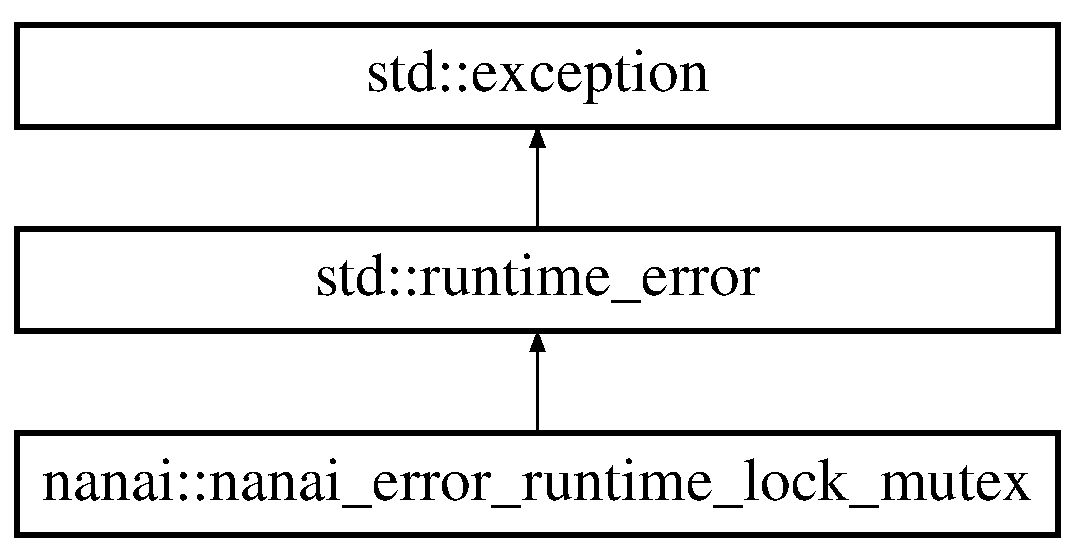
\includegraphics[height=3.000000cm]{classnanai_1_1nanai__error__runtime__lock__mutex}
\end{center}
\end{figure}
\subsection*{Public 成员函数}
\begin{DoxyCompactItemize}
\item 
\hyperlink{classnanai_1_1nanai__error__runtime__lock__mutex_ab4db66d8a33d10c1cfffc880adba1d2f}{nanai\+\_\+error\+\_\+runtime\+\_\+lock\+\_\+mutex} ()
\end{DoxyCompactItemize}
\subsection*{Public 属性}
\begin{DoxyCompactItemize}
\item 
int \hyperlink{classnanai_1_1nanai__error__runtime__lock__mutex_ab01eae05d07fbef9dc8badb4d9aa1b05}{\+\_\+errcode}
\end{DoxyCompactItemize}


\subsection{详细描述}


在文件 nanai\+\_\+object.\+h 第 106 行定义.



\subsection{构造及析构函数说明}
\hypertarget{classnanai_1_1nanai__error__runtime__lock__mutex_ab4db66d8a33d10c1cfffc880adba1d2f}{}\index{nanai\+::nanai\+\_\+error\+\_\+runtime\+\_\+lock\+\_\+mutex@{nanai\+::nanai\+\_\+error\+\_\+runtime\+\_\+lock\+\_\+mutex}!nanai\+\_\+error\+\_\+runtime\+\_\+lock\+\_\+mutex@{nanai\+\_\+error\+\_\+runtime\+\_\+lock\+\_\+mutex}}
\index{nanai\+\_\+error\+\_\+runtime\+\_\+lock\+\_\+mutex@{nanai\+\_\+error\+\_\+runtime\+\_\+lock\+\_\+mutex}!nanai\+::nanai\+\_\+error\+\_\+runtime\+\_\+lock\+\_\+mutex@{nanai\+::nanai\+\_\+error\+\_\+runtime\+\_\+lock\+\_\+mutex}}
\subsubsection[{nanai\+\_\+error\+\_\+runtime\+\_\+lock\+\_\+mutex()}]{\setlength{\rightskip}{0pt plus 5cm}nanai\+::nanai\+\_\+error\+\_\+runtime\+\_\+lock\+\_\+mutex\+::nanai\+\_\+error\+\_\+runtime\+\_\+lock\+\_\+mutex (
\begin{DoxyParamCaption}
{}
\end{DoxyParamCaption}
)\hspace{0.3cm}{\ttfamily [explicit]}}\label{classnanai_1_1nanai__error__runtime__lock__mutex_ab4db66d8a33d10c1cfffc880adba1d2f}


在文件 nanai\+\_\+object.\+cc 第 47 行定义.



\subsection{类成员变量说明}
\hypertarget{classnanai_1_1nanai__error__runtime__lock__mutex_ab01eae05d07fbef9dc8badb4d9aa1b05}{}\index{nanai\+::nanai\+\_\+error\+\_\+runtime\+\_\+lock\+\_\+mutex@{nanai\+::nanai\+\_\+error\+\_\+runtime\+\_\+lock\+\_\+mutex}!\+\_\+errcode@{\+\_\+errcode}}
\index{\+\_\+errcode@{\+\_\+errcode}!nanai\+::nanai\+\_\+error\+\_\+runtime\+\_\+lock\+\_\+mutex@{nanai\+::nanai\+\_\+error\+\_\+runtime\+\_\+lock\+\_\+mutex}}
\subsubsection[{\+\_\+errcode}]{\setlength{\rightskip}{0pt plus 5cm}int nanai\+::nanai\+\_\+error\+\_\+runtime\+\_\+lock\+\_\+mutex\+::\+\_\+errcode}\label{classnanai_1_1nanai__error__runtime__lock__mutex_ab01eae05d07fbef9dc8badb4d9aa1b05}


在文件 nanai\+\_\+object.\+h 第 110 行定义.



该类的文档由以下文件生成\+:\begin{DoxyCompactItemize}
\item 
inc/\hyperlink{nanai__object_8h}{nanai\+\_\+object.\+h}\item 
src/\hyperlink{nanai__object_8cc}{nanai\+\_\+object.\+cc}\end{DoxyCompactItemize}

\hypertarget{classnanai_1_1nanai__error__runtime__open__file}{}\section{nanai\+:\+:nanai\+\_\+error\+\_\+runtime\+\_\+open\+\_\+file类 参考}
\label{classnanai_1_1nanai__error__runtime__open__file}\index{nanai\+::nanai\+\_\+error\+\_\+runtime\+\_\+open\+\_\+file@{nanai\+::nanai\+\_\+error\+\_\+runtime\+\_\+open\+\_\+file}}


{\ttfamily \#include $<$nanai\+\_\+object.\+h$>$}

类 nanai\+:\+:nanai\+\_\+error\+\_\+runtime\+\_\+open\+\_\+file 继承关系图\+:\begin{figure}[H]
\begin{center}
\leavevmode
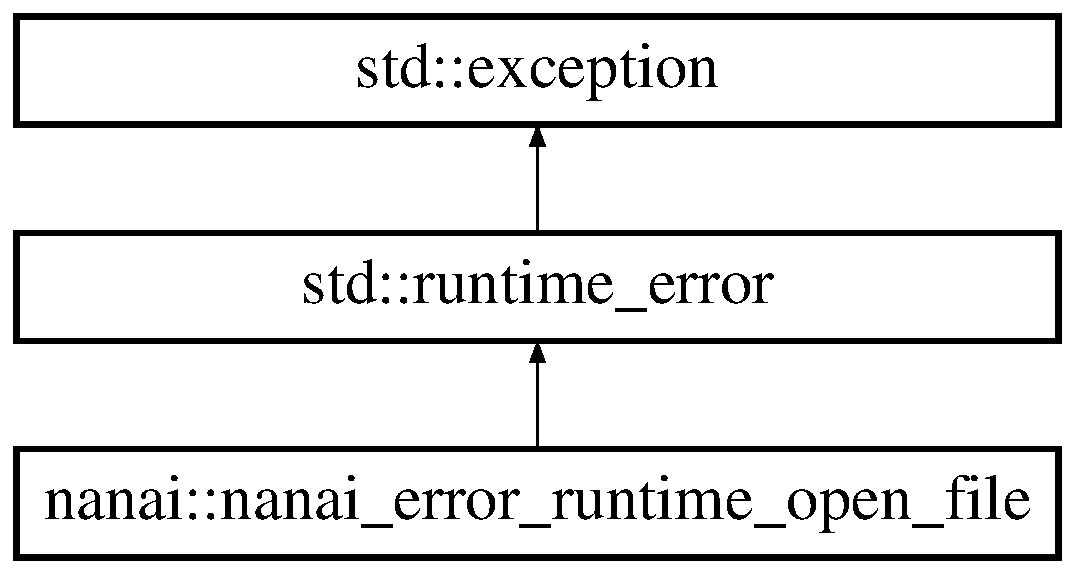
\includegraphics[height=3.000000cm]{classnanai_1_1nanai__error__runtime__open__file}
\end{center}
\end{figure}
\subsection*{Public 成员函数}
\begin{DoxyCompactItemize}
\item 
\hyperlink{classnanai_1_1nanai__error__runtime__open__file_a7ecafd733718b1371cd049961c862bd2}{nanai\+\_\+error\+\_\+runtime\+\_\+open\+\_\+file} ()
\end{DoxyCompactItemize}
\subsection*{Public 属性}
\begin{DoxyCompactItemize}
\item 
int \hyperlink{classnanai_1_1nanai__error__runtime__open__file_a60f374c9a5f457328bf76a8576a61646}{\+\_\+errcode}
\end{DoxyCompactItemize}


\subsection{详细描述}


在文件 nanai\+\_\+object.\+h 第 127 行定义.



\subsection{构造及析构函数说明}
\hypertarget{classnanai_1_1nanai__error__runtime__open__file_a7ecafd733718b1371cd049961c862bd2}{}\index{nanai\+::nanai\+\_\+error\+\_\+runtime\+\_\+open\+\_\+file@{nanai\+::nanai\+\_\+error\+\_\+runtime\+\_\+open\+\_\+file}!nanai\+\_\+error\+\_\+runtime\+\_\+open\+\_\+file@{nanai\+\_\+error\+\_\+runtime\+\_\+open\+\_\+file}}
\index{nanai\+\_\+error\+\_\+runtime\+\_\+open\+\_\+file@{nanai\+\_\+error\+\_\+runtime\+\_\+open\+\_\+file}!nanai\+::nanai\+\_\+error\+\_\+runtime\+\_\+open\+\_\+file@{nanai\+::nanai\+\_\+error\+\_\+runtime\+\_\+open\+\_\+file}}
\subsubsection[{nanai\+\_\+error\+\_\+runtime\+\_\+open\+\_\+file()}]{\setlength{\rightskip}{0pt plus 5cm}nanai\+::nanai\+\_\+error\+\_\+runtime\+\_\+open\+\_\+file\+::nanai\+\_\+error\+\_\+runtime\+\_\+open\+\_\+file (
\begin{DoxyParamCaption}
{}
\end{DoxyParamCaption}
)\hspace{0.3cm}{\ttfamily [explicit]}}\label{classnanai_1_1nanai__error__runtime__open__file_a7ecafd733718b1371cd049961c862bd2}


在文件 nanai\+\_\+object.\+cc 第 59 行定义.



\subsection{类成员变量说明}
\hypertarget{classnanai_1_1nanai__error__runtime__open__file_a60f374c9a5f457328bf76a8576a61646}{}\index{nanai\+::nanai\+\_\+error\+\_\+runtime\+\_\+open\+\_\+file@{nanai\+::nanai\+\_\+error\+\_\+runtime\+\_\+open\+\_\+file}!\+\_\+errcode@{\+\_\+errcode}}
\index{\+\_\+errcode@{\+\_\+errcode}!nanai\+::nanai\+\_\+error\+\_\+runtime\+\_\+open\+\_\+file@{nanai\+::nanai\+\_\+error\+\_\+runtime\+\_\+open\+\_\+file}}
\subsubsection[{\+\_\+errcode}]{\setlength{\rightskip}{0pt plus 5cm}int nanai\+::nanai\+\_\+error\+\_\+runtime\+\_\+open\+\_\+file\+::\+\_\+errcode}\label{classnanai_1_1nanai__error__runtime__open__file_a60f374c9a5f457328bf76a8576a61646}


在文件 nanai\+\_\+object.\+h 第 131 行定义.



该类的文档由以下文件生成\+:\begin{DoxyCompactItemize}
\item 
inc/\hyperlink{nanai__object_8h}{nanai\+\_\+object.\+h}\item 
src/\hyperlink{nanai__object_8cc}{nanai\+\_\+object.\+cc}\end{DoxyCompactItemize}

\hypertarget{classnanai_1_1nanai__error__runtime__unlock__mutex}{}\section{nanai\+:\+:nanai\+\_\+error\+\_\+runtime\+\_\+unlock\+\_\+mutex类 参考}
\label{classnanai_1_1nanai__error__runtime__unlock__mutex}\index{nanai\+::nanai\+\_\+error\+\_\+runtime\+\_\+unlock\+\_\+mutex@{nanai\+::nanai\+\_\+error\+\_\+runtime\+\_\+unlock\+\_\+mutex}}


{\ttfamily \#include $<$nanai\+\_\+object.\+h$>$}

类 nanai\+:\+:nanai\+\_\+error\+\_\+runtime\+\_\+unlock\+\_\+mutex 继承关系图\+:\begin{figure}[H]
\begin{center}
\leavevmode
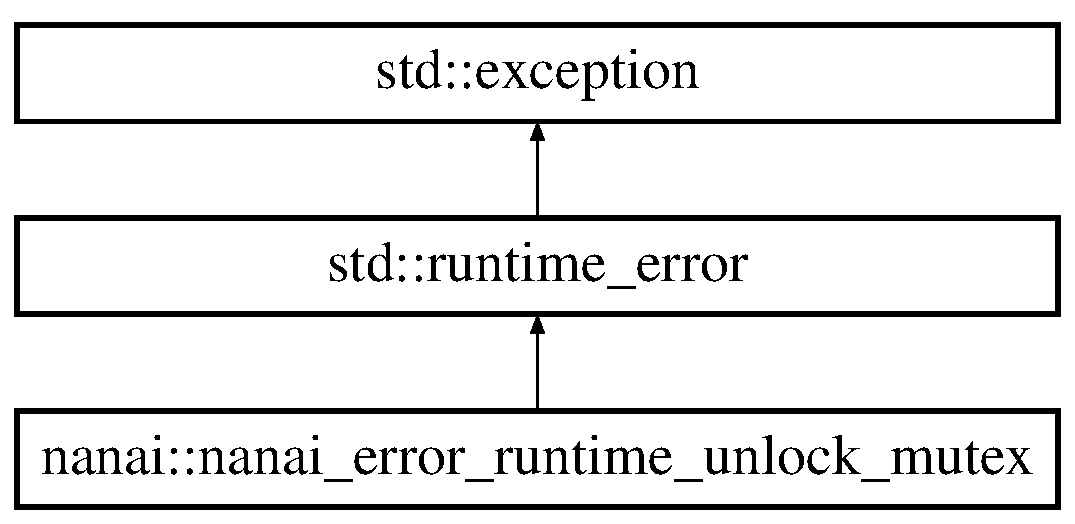
\includegraphics[height=3.000000cm]{classnanai_1_1nanai__error__runtime__unlock__mutex}
\end{center}
\end{figure}
\subsection*{Public 成员函数}
\begin{DoxyCompactItemize}
\item 
\hyperlink{classnanai_1_1nanai__error__runtime__unlock__mutex_a7f077e10b1c5ecf91f7b001d4bf5436f}{nanai\+\_\+error\+\_\+runtime\+\_\+unlock\+\_\+mutex} ()
\end{DoxyCompactItemize}
\subsection*{Public 属性}
\begin{DoxyCompactItemize}
\item 
int \hyperlink{classnanai_1_1nanai__error__runtime__unlock__mutex_aba361f162e36f4a3a7d9028832bf65e6}{\+\_\+errcode}
\end{DoxyCompactItemize}


\subsection{详细描述}


在文件 nanai\+\_\+object.\+h 第 113 行定义.



\subsection{构造及析构函数说明}
\hypertarget{classnanai_1_1nanai__error__runtime__unlock__mutex_a7f077e10b1c5ecf91f7b001d4bf5436f}{}\index{nanai\+::nanai\+\_\+error\+\_\+runtime\+\_\+unlock\+\_\+mutex@{nanai\+::nanai\+\_\+error\+\_\+runtime\+\_\+unlock\+\_\+mutex}!nanai\+\_\+error\+\_\+runtime\+\_\+unlock\+\_\+mutex@{nanai\+\_\+error\+\_\+runtime\+\_\+unlock\+\_\+mutex}}
\index{nanai\+\_\+error\+\_\+runtime\+\_\+unlock\+\_\+mutex@{nanai\+\_\+error\+\_\+runtime\+\_\+unlock\+\_\+mutex}!nanai\+::nanai\+\_\+error\+\_\+runtime\+\_\+unlock\+\_\+mutex@{nanai\+::nanai\+\_\+error\+\_\+runtime\+\_\+unlock\+\_\+mutex}}
\subsubsection[{nanai\+\_\+error\+\_\+runtime\+\_\+unlock\+\_\+mutex()}]{\setlength{\rightskip}{0pt plus 5cm}nanai\+::nanai\+\_\+error\+\_\+runtime\+\_\+unlock\+\_\+mutex\+::nanai\+\_\+error\+\_\+runtime\+\_\+unlock\+\_\+mutex (
\begin{DoxyParamCaption}
{}
\end{DoxyParamCaption}
)\hspace{0.3cm}{\ttfamily [explicit]}}\label{classnanai_1_1nanai__error__runtime__unlock__mutex_a7f077e10b1c5ecf91f7b001d4bf5436f}


在文件 nanai\+\_\+object.\+cc 第 51 行定义.



\subsection{类成员变量说明}
\hypertarget{classnanai_1_1nanai__error__runtime__unlock__mutex_aba361f162e36f4a3a7d9028832bf65e6}{}\index{nanai\+::nanai\+\_\+error\+\_\+runtime\+\_\+unlock\+\_\+mutex@{nanai\+::nanai\+\_\+error\+\_\+runtime\+\_\+unlock\+\_\+mutex}!\+\_\+errcode@{\+\_\+errcode}}
\index{\+\_\+errcode@{\+\_\+errcode}!nanai\+::nanai\+\_\+error\+\_\+runtime\+\_\+unlock\+\_\+mutex@{nanai\+::nanai\+\_\+error\+\_\+runtime\+\_\+unlock\+\_\+mutex}}
\subsubsection[{\+\_\+errcode}]{\setlength{\rightskip}{0pt plus 5cm}int nanai\+::nanai\+\_\+error\+\_\+runtime\+\_\+unlock\+\_\+mutex\+::\+\_\+errcode}\label{classnanai_1_1nanai__error__runtime__unlock__mutex_aba361f162e36f4a3a7d9028832bf65e6}


在文件 nanai\+\_\+object.\+h 第 117 行定义.



该类的文档由以下文件生成\+:\begin{DoxyCompactItemize}
\item 
inc/\hyperlink{nanai__object_8h}{nanai\+\_\+object.\+h}\item 
src/\hyperlink{nanai__object_8cc}{nanai\+\_\+object.\+cc}\end{DoxyCompactItemize}

\hypertarget{classnanai_1_1nanai__error__unknow__error}{}\section{nanai\+:\+:nanai\+\_\+error\+\_\+unknow\+\_\+error类 参考}
\label{classnanai_1_1nanai__error__unknow__error}\index{nanai\+::nanai\+\_\+error\+\_\+unknow\+\_\+error@{nanai\+::nanai\+\_\+error\+\_\+unknow\+\_\+error}}


{\ttfamily \#include $<$nanai\+\_\+object.\+h$>$}

类 nanai\+:\+:nanai\+\_\+error\+\_\+unknow\+\_\+error 继承关系图\+:\begin{figure}[H]
\begin{center}
\leavevmode
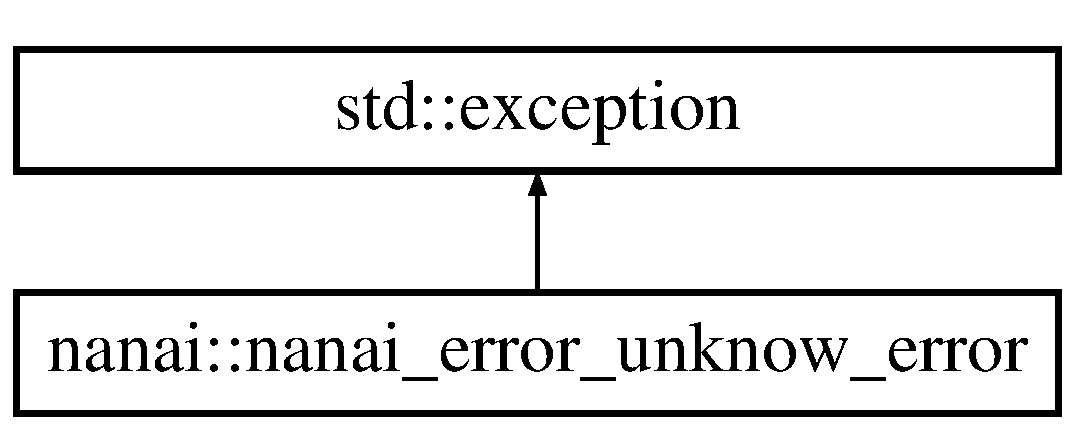
\includegraphics[height=2.000000cm]{classnanai_1_1nanai__error__unknow__error}
\end{center}
\end{figure}
\subsection*{Public 成员函数}
\begin{DoxyCompactItemize}
\item 
\hyperlink{classnanai_1_1nanai__error__unknow__error_afdeee689504293bd5d7ff4950c32b709}{nanai\+\_\+error\+\_\+unknow\+\_\+error} ()
\item 
virtual const char $\ast$ \hyperlink{classnanai_1_1nanai__error__unknow__error_a4e27460d5ed88e9cb297499c5c213253}{what} () const \hyperlink{nanai__object_8h_ad7597118202b58872a4a874eab3dc1a2}{\+\_\+\+N\+O\+E\+X\+C\+E\+P\+T}
\end{DoxyCompactItemize}
\subsection*{Public 属性}
\begin{DoxyCompactItemize}
\item 
int \hyperlink{classnanai_1_1nanai__error__unknow__error_a1d843ccc2365e828549cfea01bab26f8}{\+\_\+errcode}
\end{DoxyCompactItemize}


\subsection{详细描述}


在文件 nanai\+\_\+object.\+h 第 34 行定义.



\subsection{构造及析构函数说明}
\hypertarget{classnanai_1_1nanai__error__unknow__error_afdeee689504293bd5d7ff4950c32b709}{}\index{nanai\+::nanai\+\_\+error\+\_\+unknow\+\_\+error@{nanai\+::nanai\+\_\+error\+\_\+unknow\+\_\+error}!nanai\+\_\+error\+\_\+unknow\+\_\+error@{nanai\+\_\+error\+\_\+unknow\+\_\+error}}
\index{nanai\+\_\+error\+\_\+unknow\+\_\+error@{nanai\+\_\+error\+\_\+unknow\+\_\+error}!nanai\+::nanai\+\_\+error\+\_\+unknow\+\_\+error@{nanai\+::nanai\+\_\+error\+\_\+unknow\+\_\+error}}
\subsubsection[{nanai\+\_\+error\+\_\+unknow\+\_\+error()}]{\setlength{\rightskip}{0pt plus 5cm}nanai\+::nanai\+\_\+error\+\_\+unknow\+\_\+error\+::nanai\+\_\+error\+\_\+unknow\+\_\+error (
\begin{DoxyParamCaption}
{}
\end{DoxyParamCaption}
)\hspace{0.3cm}{\ttfamily [explicit]}}\label{classnanai_1_1nanai__error__unknow__error_afdeee689504293bd5d7ff4950c32b709}


在文件 nanai\+\_\+object.\+cc 第 6 行定义.



\subsection{成员函数说明}
\hypertarget{classnanai_1_1nanai__error__unknow__error_a4e27460d5ed88e9cb297499c5c213253}{}\index{nanai\+::nanai\+\_\+error\+\_\+unknow\+\_\+error@{nanai\+::nanai\+\_\+error\+\_\+unknow\+\_\+error}!what@{what}}
\index{what@{what}!nanai\+::nanai\+\_\+error\+\_\+unknow\+\_\+error@{nanai\+::nanai\+\_\+error\+\_\+unknow\+\_\+error}}
\subsubsection[{what() const \+\_\+\+N\+O\+E\+X\+C\+E\+P\+T}]{\setlength{\rightskip}{0pt plus 5cm}const char $\ast$ nanai\+::nanai\+\_\+error\+\_\+unknow\+\_\+error\+::what (
\begin{DoxyParamCaption}
{}
\end{DoxyParamCaption}
) const\hspace{0.3cm}{\ttfamily [virtual]}}\label{classnanai_1_1nanai__error__unknow__error_a4e27460d5ed88e9cb297499c5c213253}


在文件 nanai\+\_\+object.\+cc 第 9 行定义.



\subsection{类成员变量说明}
\hypertarget{classnanai_1_1nanai__error__unknow__error_a1d843ccc2365e828549cfea01bab26f8}{}\index{nanai\+::nanai\+\_\+error\+\_\+unknow\+\_\+error@{nanai\+::nanai\+\_\+error\+\_\+unknow\+\_\+error}!\+\_\+errcode@{\+\_\+errcode}}
\index{\+\_\+errcode@{\+\_\+errcode}!nanai\+::nanai\+\_\+error\+\_\+unknow\+\_\+error@{nanai\+::nanai\+\_\+error\+\_\+unknow\+\_\+error}}
\subsubsection[{\+\_\+errcode}]{\setlength{\rightskip}{0pt plus 5cm}int nanai\+::nanai\+\_\+error\+\_\+unknow\+\_\+error\+::\+\_\+errcode}\label{classnanai_1_1nanai__error__unknow__error_a1d843ccc2365e828549cfea01bab26f8}


在文件 nanai\+\_\+object.\+h 第 39 行定义.



该类的文档由以下文件生成\+:\begin{DoxyCompactItemize}
\item 
inc/\hyperlink{nanai__object_8h}{nanai\+\_\+object.\+h}\item 
src/\hyperlink{nanai__object_8cc}{nanai\+\_\+object.\+cc}\end{DoxyCompactItemize}

\hypertarget{classnanai_1_1nanai__object}{}\section{nanai\+:\+:nanai\+\_\+object类 参考}
\label{classnanai_1_1nanai__object}\index{nanai\+::nanai\+\_\+object@{nanai\+::nanai\+\_\+object}}


{\ttfamily \#include $<$nanai\+\_\+object.\+h$>$}

类 nanai\+:\+:nanai\+\_\+object 继承关系图\+:\begin{figure}[H]
\begin{center}
\leavevmode
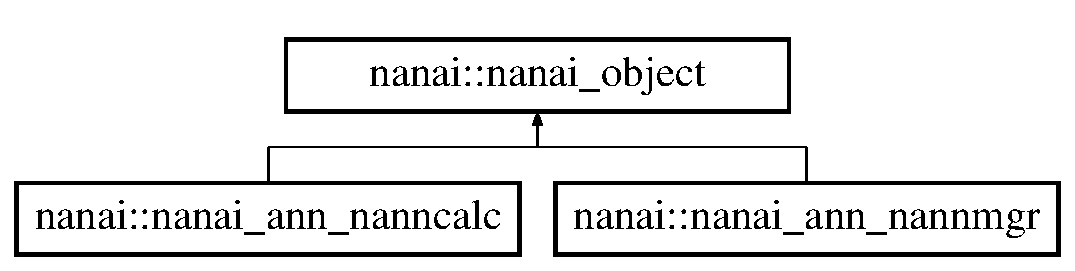
\includegraphics[height=2.000000cm]{classnanai_1_1nanai__object}
\end{center}
\end{figure}
\subsection*{Public 成员函数}
\begin{DoxyCompactItemize}
\item 
\hyperlink{classnanai_1_1nanai__object_a066d094b5abc020f08b38ee92220da6a}{nanai\+\_\+object} ()
\item 
\hyperlink{classnanai_1_1nanai__object_a2c2b99938e659b07204690ab51b148c7}{nanai\+\_\+object} (const \hyperlink{classnanai_1_1nanai__object}{nanai\+\_\+object} \&t)
\item 
virtual \hyperlink{classnanai_1_1nanai__object_a7aaa650c4408749ac7e0ca70547920ee}{$\sim$nanai\+\_\+object} ()
\item 
int \hyperlink{classnanai_1_1nanai__object_ab70ce957f8be26e1a4c61461de9c4aa7}{get\+\_\+last\+\_\+error} () const 
\item 
void \hyperlink{classnanai_1_1nanai__object_a9b05c72f0058867e692dcbba020436c6}{error} (int err)
\end{DoxyCompactItemize}
\subsection*{Protected 成员函数}
\begin{DoxyCompactItemize}
\item 
virtual void \hyperlink{classnanai_1_1nanai__object_a87f162335cead23a1409f7c0570a3284}{on\+\_\+error} (int err)
\end{DoxyCompactItemize}
\subsection*{Protected 属性}
\begin{DoxyCompactItemize}
\item 
int \hyperlink{classnanai_1_1nanai__object_affc3fedffe027488da1cd445291504b3}{\+\_\+last\+\_\+error}
\end{DoxyCompactItemize}


\subsection{详细描述}


在文件 nanai\+\_\+object.\+h 第 141 行定义.



\subsection{构造及析构函数说明}
\hypertarget{classnanai_1_1nanai__object_a066d094b5abc020f08b38ee92220da6a}{}\index{nanai\+::nanai\+\_\+object@{nanai\+::nanai\+\_\+object}!nanai\+\_\+object@{nanai\+\_\+object}}
\index{nanai\+\_\+object@{nanai\+\_\+object}!nanai\+::nanai\+\_\+object@{nanai\+::nanai\+\_\+object}}
\subsubsection[{nanai\+\_\+object()}]{\setlength{\rightskip}{0pt plus 5cm}nanai\+::nanai\+\_\+object\+::nanai\+\_\+object (
\begin{DoxyParamCaption}
{}
\end{DoxyParamCaption}
)}\label{classnanai_1_1nanai__object_a066d094b5abc020f08b38ee92220da6a}


在文件 nanai\+\_\+object.\+cc 第 102 行定义.

\hypertarget{classnanai_1_1nanai__object_a2c2b99938e659b07204690ab51b148c7}{}\index{nanai\+::nanai\+\_\+object@{nanai\+::nanai\+\_\+object}!nanai\+\_\+object@{nanai\+\_\+object}}
\index{nanai\+\_\+object@{nanai\+\_\+object}!nanai\+::nanai\+\_\+object@{nanai\+::nanai\+\_\+object}}
\subsubsection[{nanai\+\_\+object(const nanai\+\_\+object \&t)}]{\setlength{\rightskip}{0pt plus 5cm}nanai\+::nanai\+\_\+object\+::nanai\+\_\+object (
\begin{DoxyParamCaption}
\item[{const {\bf nanai\+\_\+object} \&}]{t}
\end{DoxyParamCaption}
)}\label{classnanai_1_1nanai__object_a2c2b99938e659b07204690ab51b148c7}


在文件 nanai\+\_\+object.\+cc 第 106 行定义.

\hypertarget{classnanai_1_1nanai__object_a7aaa650c4408749ac7e0ca70547920ee}{}\index{nanai\+::nanai\+\_\+object@{nanai\+::nanai\+\_\+object}!````~nanai\+\_\+object@{$\sim$nanai\+\_\+object}}
\index{````~nanai\+\_\+object@{$\sim$nanai\+\_\+object}!nanai\+::nanai\+\_\+object@{nanai\+::nanai\+\_\+object}}
\subsubsection[{$\sim$nanai\+\_\+object()}]{\setlength{\rightskip}{0pt plus 5cm}nanai\+::nanai\+\_\+object\+::$\sim$nanai\+\_\+object (
\begin{DoxyParamCaption}
{}
\end{DoxyParamCaption}
)\hspace{0.3cm}{\ttfamily [virtual]}}\label{classnanai_1_1nanai__object_a7aaa650c4408749ac7e0ca70547920ee}


在文件 nanai\+\_\+object.\+cc 第 110 行定义.



\subsection{成员函数说明}
\hypertarget{classnanai_1_1nanai__object_a9b05c72f0058867e692dcbba020436c6}{}\index{nanai\+::nanai\+\_\+object@{nanai\+::nanai\+\_\+object}!error@{error}}
\index{error@{error}!nanai\+::nanai\+\_\+object@{nanai\+::nanai\+\_\+object}}
\subsubsection[{error(int err)}]{\setlength{\rightskip}{0pt plus 5cm}void nanai\+::nanai\+\_\+object\+::error (
\begin{DoxyParamCaption}
\item[{int}]{err}
\end{DoxyParamCaption}
)}\label{classnanai_1_1nanai__object_a9b05c72f0058867e692dcbba020436c6}


在文件 nanai\+\_\+object.\+cc 第 121 行定义.

\hypertarget{classnanai_1_1nanai__object_ab70ce957f8be26e1a4c61461de9c4aa7}{}\index{nanai\+::nanai\+\_\+object@{nanai\+::nanai\+\_\+object}!get\+\_\+last\+\_\+error@{get\+\_\+last\+\_\+error}}
\index{get\+\_\+last\+\_\+error@{get\+\_\+last\+\_\+error}!nanai\+::nanai\+\_\+object@{nanai\+::nanai\+\_\+object}}
\subsubsection[{get\+\_\+last\+\_\+error() const }]{\setlength{\rightskip}{0pt plus 5cm}int nanai\+::nanai\+\_\+object\+::get\+\_\+last\+\_\+error (
\begin{DoxyParamCaption}
{}
\end{DoxyParamCaption}
) const}\label{classnanai_1_1nanai__object_ab70ce957f8be26e1a4c61461de9c4aa7}


在文件 nanai\+\_\+object.\+cc 第 117 行定义.

\hypertarget{classnanai_1_1nanai__object_a87f162335cead23a1409f7c0570a3284}{}\index{nanai\+::nanai\+\_\+object@{nanai\+::nanai\+\_\+object}!on\+\_\+error@{on\+\_\+error}}
\index{on\+\_\+error@{on\+\_\+error}!nanai\+::nanai\+\_\+object@{nanai\+::nanai\+\_\+object}}
\subsubsection[{on\+\_\+error(int err)}]{\setlength{\rightskip}{0pt plus 5cm}void nanai\+::nanai\+\_\+object\+::on\+\_\+error (
\begin{DoxyParamCaption}
\item[{int}]{err}
\end{DoxyParamCaption}
)\hspace{0.3cm}{\ttfamily [protected]}, {\ttfamily [virtual]}}\label{classnanai_1_1nanai__object_a87f162335cead23a1409f7c0570a3284}


被 \hyperlink{classnanai_1_1nanai__ann__nannmgr_a28ea36058e9dfd5ce6b80d6011931acc}{nanai\+::nanai\+\_\+ann\+\_\+nannmgr} , 以及 \hyperlink{classnanai_1_1nanai__ann__nanncalc_a675afb775a34013e6aff1f8d669e7de0}{nanai\+::nanai\+\_\+ann\+\_\+nanncalc} 重载.



在文件 nanai\+\_\+object.\+cc 第 113 行定义.



\subsection{类成员变量说明}
\hypertarget{classnanai_1_1nanai__object_affc3fedffe027488da1cd445291504b3}{}\index{nanai\+::nanai\+\_\+object@{nanai\+::nanai\+\_\+object}!\+\_\+last\+\_\+error@{\+\_\+last\+\_\+error}}
\index{\+\_\+last\+\_\+error@{\+\_\+last\+\_\+error}!nanai\+::nanai\+\_\+object@{nanai\+::nanai\+\_\+object}}
\subsubsection[{\+\_\+last\+\_\+error}]{\setlength{\rightskip}{0pt plus 5cm}int nanai\+::nanai\+\_\+object\+::\+\_\+last\+\_\+error\hspace{0.3cm}{\ttfamily [protected]}}\label{classnanai_1_1nanai__object_affc3fedffe027488da1cd445291504b3}


在文件 nanai\+\_\+object.\+h 第 155 行定义.



该类的文档由以下文件生成\+:\begin{DoxyCompactItemize}
\item 
inc/\hyperlink{nanai__object_8h}{nanai\+\_\+object.\+h}\item 
src/\hyperlink{nanai__object_8cc}{nanai\+\_\+object.\+cc}\end{DoxyCompactItemize}

\hypertarget{classnanmath_1_1nanmath__matrix}{}\section{nanmath\+:\+:nanmath\+\_\+matrix类 参考}
\label{classnanmath_1_1nanmath__matrix}\index{nanmath\+::nanmath\+\_\+matrix@{nanmath\+::nanmath\+\_\+matrix}}


{\ttfamily \#include $<$nanmath\+\_\+matrix.\+h$>$}

\subsection*{Public 成员函数}
\begin{DoxyCompactItemize}
\item 
\hyperlink{classnanmath_1_1nanmath__matrix_a4f0a09745fd4a7563a9462358a4cf9f3}{nanmath\+\_\+matrix} ()
\item 
\hyperlink{classnanmath_1_1nanmath__matrix_a16873cc6b8741de29e1d7a596ee8836c}{nanmath\+\_\+matrix} (size\+\_\+t r, size\+\_\+t c)
\item 
\hyperlink{classnanmath_1_1nanmath__matrix_ad2712c998744cec123026fe3cbb7b5da}{nanmath\+\_\+matrix} (const std\+::vector$<$ std\+::vector$<$ double $>$ $>$ \&mat)
\item 
\hyperlink{classnanmath_1_1nanmath__matrix_aa0a5698fe01db8ee25bd9d8fbe646628}{nanmath\+\_\+matrix} (const \hyperlink{classnanmath_1_1nanmath__matrix}{nanmath\+\_\+matrix} \&t)
\item 
virtual \hyperlink{classnanmath_1_1nanmath__matrix_a41cc1dac91f6ef08f9b3ec1baf1af3e3}{$\sim$nanmath\+\_\+matrix} ()
\item 
virtual void \hyperlink{classnanmath_1_1nanmath__matrix_a0d9762b03f6e27563bbdf821be78342d}{create} (size\+\_\+t r, size\+\_\+t c)
\item 
virtual void \hyperlink{classnanmath_1_1nanmath__matrix_a8a1432e6ebd91c5035285ee47c747798}{destroy} ()
\item 
virtual void \hyperlink{classnanmath_1_1nanmath__matrix_a65c42ef1d4dca4553ffd13fcc0258a74}{clear} ()
\item 
virtual double \hyperlink{classnanmath_1_1nanmath__matrix_abeecd392efba8d91e4f0e1151199d063}{at} (size\+\_\+t r, size\+\_\+t c) const 
\item 
virtual size\+\_\+t \hyperlink{classnanmath_1_1nanmath__matrix_a15dc80fe330112c1a17ef6f7de168943}{row\+\_\+size} () const 
\item 
virtual size\+\_\+t \hyperlink{classnanmath_1_1nanmath__matrix_a4fcc48d81fc393f7cbee5e3c1fe04f75}{col\+\_\+size} () const 
\item 
virtual void \hyperlink{classnanmath_1_1nanmath__matrix_a96c4e5fed99527adee5ff5b756589d0d}{set} (size\+\_\+t r, size\+\_\+t c, double v)
\item 
virtual void \hyperlink{classnanmath_1_1nanmath__matrix_a0074200e9eaa3ffb2b9ce6602e1bfd5d}{set} (const \hyperlink{classnanmath_1_1nanmath__matrix}{nanmath\+\_\+matrix} \&mat)
\item 
virtual void \hyperlink{classnanmath_1_1nanmath__matrix_afd46732914cf6da29d584cbbb4a47499}{set\+\_\+row} (size\+\_\+t r, const std\+::vector$<$ double $>$ \&row)
\item 
virtual void \hyperlink{classnanmath_1_1nanmath__matrix_af5eea2f6b98686e9b243c02513908d16}{set\+\_\+col} (size\+\_\+t c, const std\+::vector$<$ double $>$ \&col)
\item 
virtual void \hyperlink{classnanmath_1_1nanmath__matrix_a2611cc9aef30706e7f11e15cd2405699}{push\+\_\+row} (const std\+::vector$<$ double $>$ \&row)
\item 
virtual std\+::vector$<$ std\+::vector$<$ double $>$ $>$ \hyperlink{classnanmath_1_1nanmath__matrix_aac2fd129eff7ea0248ccc49e24414454}{get} ()
\item 
virtual void \hyperlink{classnanmath_1_1nanmath__matrix_ac27e457cd31058c95b9b5ccf7b4809c0}{resize} (size\+\_\+t r, size\+\_\+t c)
\item 
virtual void \hyperlink{classnanmath_1_1nanmath__matrix_a114b8a9aa414e94b06c0ddd9496a34d8}{print} ()
\item 
virtual void \hyperlink{classnanmath_1_1nanmath__matrix_aa4dadc0c46659f398ad576eac8c3b064}{zero} ()
\item 
virtual void \hyperlink{classnanmath_1_1nanmath__matrix_a625284547b9fbbef11b331cf312cd74e}{random} (int t=0)
\item 
virtual \hyperlink{classnanmath_1_1nanmath__matrix}{nanmath\+\_\+matrix} \hyperlink{classnanmath_1_1nanmath__matrix_a1e04289b0bfb7556f2d4c25d49a8198d}{T} () const 
\item 
virtual \hyperlink{classnanmath_1_1nanmath__vector}{nanmath\+\_\+vector} \hyperlink{classnanmath_1_1nanmath__matrix_aaebae090e22fdb90b531ea376a958959}{left\+\_\+mul} (const \hyperlink{classnanmath_1_1nanmath__vector}{nanmath\+\_\+vector} \&v)
\item 
virtual \hyperlink{classnanmath_1_1nanmath__vector}{nanmath\+\_\+vector} \hyperlink{classnanmath_1_1nanmath__matrix_a785f78f5f75769e2e4d1dbe23c37ea2a}{right\+\_\+mul} (const \hyperlink{classnanmath_1_1nanmath__vector}{nanmath\+\_\+vector} \&v)
\item 
virtual \hyperlink{classnanmath_1_1nanmath__vector}{nanmath\+\_\+vector} \hyperlink{classnanmath_1_1nanmath__matrix_a947460315b7a871de1c7084cde469e3e}{mul} (const \hyperlink{classnanmath_1_1nanmath__vector}{nanmath\+\_\+vector} \&v)
\item 
virtual \hyperlink{classnanmath_1_1nanmath__matrix}{nanmath\+\_\+matrix} \hyperlink{classnanmath_1_1nanmath__matrix_aec27097c5a8ec49fd44378a3942eebb5}{mul} (const \hyperlink{classnanmath_1_1nanmath__matrix}{nanmath\+\_\+matrix} \&mat)
\item 
std\+::vector$<$ double $>$ \hyperlink{classnanmath_1_1nanmath__matrix_afb04741def3ef6e1fe2b489211d631f6}{operator\mbox{[}$\,$\mbox{]}} (size\+\_\+t r) const 
\end{DoxyCompactItemize}
\subsection*{Protected 属性}
\begin{DoxyCompactItemize}
\item 
std\+::vector$<$ std\+::vector$<$ double $>$ $>$ \hyperlink{classnanmath_1_1nanmath__matrix_a2e376e4d599abc18c1bac142dcc89ab2}{\+\_\+matrix}
\end{DoxyCompactItemize}


\subsection{详细描述}


在文件 nanmath\+\_\+matrix.\+h 第 9 行定义.



\subsection{构造及析构函数说明}
\hypertarget{classnanmath_1_1nanmath__matrix_a4f0a09745fd4a7563a9462358a4cf9f3}{}\index{nanmath\+::nanmath\+\_\+matrix@{nanmath\+::nanmath\+\_\+matrix}!nanmath\+\_\+matrix@{nanmath\+\_\+matrix}}
\index{nanmath\+\_\+matrix@{nanmath\+\_\+matrix}!nanmath\+::nanmath\+\_\+matrix@{nanmath\+::nanmath\+\_\+matrix}}
\subsubsection[{nanmath\+\_\+matrix()}]{\setlength{\rightskip}{0pt plus 5cm}nanmath\+::nanmath\+\_\+matrix\+::nanmath\+\_\+matrix (
\begin{DoxyParamCaption}
{}
\end{DoxyParamCaption}
)}\label{classnanmath_1_1nanmath__matrix_a4f0a09745fd4a7563a9462358a4cf9f3}


在文件 nanmath\+\_\+matrix.\+cc 第 12 行定义.

\hypertarget{classnanmath_1_1nanmath__matrix_a16873cc6b8741de29e1d7a596ee8836c}{}\index{nanmath\+::nanmath\+\_\+matrix@{nanmath\+::nanmath\+\_\+matrix}!nanmath\+\_\+matrix@{nanmath\+\_\+matrix}}
\index{nanmath\+\_\+matrix@{nanmath\+\_\+matrix}!nanmath\+::nanmath\+\_\+matrix@{nanmath\+::nanmath\+\_\+matrix}}
\subsubsection[{nanmath\+\_\+matrix(size\+\_\+t r, size\+\_\+t c)}]{\setlength{\rightskip}{0pt plus 5cm}nanmath\+::nanmath\+\_\+matrix\+::nanmath\+\_\+matrix (
\begin{DoxyParamCaption}
\item[{size\+\_\+t}]{r, }
\item[{size\+\_\+t}]{c}
\end{DoxyParamCaption}
)}\label{classnanmath_1_1nanmath__matrix_a16873cc6b8741de29e1d7a596ee8836c}


在文件 nanmath\+\_\+matrix.\+cc 第 15 行定义.

\hypertarget{classnanmath_1_1nanmath__matrix_ad2712c998744cec123026fe3cbb7b5da}{}\index{nanmath\+::nanmath\+\_\+matrix@{nanmath\+::nanmath\+\_\+matrix}!nanmath\+\_\+matrix@{nanmath\+\_\+matrix}}
\index{nanmath\+\_\+matrix@{nanmath\+\_\+matrix}!nanmath\+::nanmath\+\_\+matrix@{nanmath\+::nanmath\+\_\+matrix}}
\subsubsection[{nanmath\+\_\+matrix(const std\+::vector$<$ std\+::vector$<$ double $>$ $>$ \&mat)}]{\setlength{\rightskip}{0pt plus 5cm}nanmath\+::nanmath\+\_\+matrix\+::nanmath\+\_\+matrix (
\begin{DoxyParamCaption}
\item[{const std\+::vector$<$ std\+::vector$<$ double $>$ $>$ \&}]{mat}
\end{DoxyParamCaption}
)}\label{classnanmath_1_1nanmath__matrix_ad2712c998744cec123026fe3cbb7b5da}


在文件 nanmath\+\_\+matrix.\+cc 第 19 行定义.

\hypertarget{classnanmath_1_1nanmath__matrix_aa0a5698fe01db8ee25bd9d8fbe646628}{}\index{nanmath\+::nanmath\+\_\+matrix@{nanmath\+::nanmath\+\_\+matrix}!nanmath\+\_\+matrix@{nanmath\+\_\+matrix}}
\index{nanmath\+\_\+matrix@{nanmath\+\_\+matrix}!nanmath\+::nanmath\+\_\+matrix@{nanmath\+::nanmath\+\_\+matrix}}
\subsubsection[{nanmath\+\_\+matrix(const nanmath\+\_\+matrix \&t)}]{\setlength{\rightskip}{0pt plus 5cm}nanmath\+::nanmath\+\_\+matrix\+::nanmath\+\_\+matrix (
\begin{DoxyParamCaption}
\item[{const {\bf nanmath\+\_\+matrix} \&}]{t}
\end{DoxyParamCaption}
)}\label{classnanmath_1_1nanmath__matrix_aa0a5698fe01db8ee25bd9d8fbe646628}


在文件 nanmath\+\_\+matrix.\+cc 第 32 行定义.

\hypertarget{classnanmath_1_1nanmath__matrix_a41cc1dac91f6ef08f9b3ec1baf1af3e3}{}\index{nanmath\+::nanmath\+\_\+matrix@{nanmath\+::nanmath\+\_\+matrix}!````~nanmath\+\_\+matrix@{$\sim$nanmath\+\_\+matrix}}
\index{````~nanmath\+\_\+matrix@{$\sim$nanmath\+\_\+matrix}!nanmath\+::nanmath\+\_\+matrix@{nanmath\+::nanmath\+\_\+matrix}}
\subsubsection[{$\sim$nanmath\+\_\+matrix()}]{\setlength{\rightskip}{0pt plus 5cm}nanmath\+::nanmath\+\_\+matrix\+::$\sim$nanmath\+\_\+matrix (
\begin{DoxyParamCaption}
{}
\end{DoxyParamCaption}
)\hspace{0.3cm}{\ttfamily [virtual]}}\label{classnanmath_1_1nanmath__matrix_a41cc1dac91f6ef08f9b3ec1baf1af3e3}


在文件 nanmath\+\_\+matrix.\+cc 第 36 行定义.



\subsection{成员函数说明}
\hypertarget{classnanmath_1_1nanmath__matrix_abeecd392efba8d91e4f0e1151199d063}{}\index{nanmath\+::nanmath\+\_\+matrix@{nanmath\+::nanmath\+\_\+matrix}!at@{at}}
\index{at@{at}!nanmath\+::nanmath\+\_\+matrix@{nanmath\+::nanmath\+\_\+matrix}}
\subsubsection[{at(size\+\_\+t r, size\+\_\+t c) const }]{\setlength{\rightskip}{0pt plus 5cm}double nanmath\+::nanmath\+\_\+matrix\+::at (
\begin{DoxyParamCaption}
\item[{size\+\_\+t}]{r, }
\item[{size\+\_\+t}]{c}
\end{DoxyParamCaption}
) const\hspace{0.3cm}{\ttfamily [virtual]}}\label{classnanmath_1_1nanmath__matrix_abeecd392efba8d91e4f0e1151199d063}


在文件 nanmath\+\_\+matrix.\+cc 第 63 行定义.

\hypertarget{classnanmath_1_1nanmath__matrix_a65c42ef1d4dca4553ffd13fcc0258a74}{}\index{nanmath\+::nanmath\+\_\+matrix@{nanmath\+::nanmath\+\_\+matrix}!clear@{clear}}
\index{clear@{clear}!nanmath\+::nanmath\+\_\+matrix@{nanmath\+::nanmath\+\_\+matrix}}
\subsubsection[{clear()}]{\setlength{\rightskip}{0pt plus 5cm}void nanmath\+::nanmath\+\_\+matrix\+::clear (
\begin{DoxyParamCaption}
{}
\end{DoxyParamCaption}
)\hspace{0.3cm}{\ttfamily [virtual]}}\label{classnanmath_1_1nanmath__matrix_a65c42ef1d4dca4553ffd13fcc0258a74}


在文件 nanmath\+\_\+matrix.\+cc 第 59 行定义.

\hypertarget{classnanmath_1_1nanmath__matrix_a4fcc48d81fc393f7cbee5e3c1fe04f75}{}\index{nanmath\+::nanmath\+\_\+matrix@{nanmath\+::nanmath\+\_\+matrix}!col\+\_\+size@{col\+\_\+size}}
\index{col\+\_\+size@{col\+\_\+size}!nanmath\+::nanmath\+\_\+matrix@{nanmath\+::nanmath\+\_\+matrix}}
\subsubsection[{col\+\_\+size() const }]{\setlength{\rightskip}{0pt plus 5cm}size\+\_\+t nanmath\+::nanmath\+\_\+matrix\+::col\+\_\+size (
\begin{DoxyParamCaption}
{}
\end{DoxyParamCaption}
) const\hspace{0.3cm}{\ttfamily [virtual]}}\label{classnanmath_1_1nanmath__matrix_a4fcc48d81fc393f7cbee5e3c1fe04f75}


在文件 nanmath\+\_\+matrix.\+cc 第 78 行定义.

\hypertarget{classnanmath_1_1nanmath__matrix_a0d9762b03f6e27563bbdf821be78342d}{}\index{nanmath\+::nanmath\+\_\+matrix@{nanmath\+::nanmath\+\_\+matrix}!create@{create}}
\index{create@{create}!nanmath\+::nanmath\+\_\+matrix@{nanmath\+::nanmath\+\_\+matrix}}
\subsubsection[{create(size\+\_\+t r, size\+\_\+t c)}]{\setlength{\rightskip}{0pt plus 5cm}void nanmath\+::nanmath\+\_\+matrix\+::create (
\begin{DoxyParamCaption}
\item[{size\+\_\+t}]{r, }
\item[{size\+\_\+t}]{c}
\end{DoxyParamCaption}
)\hspace{0.3cm}{\ttfamily [virtual]}}\label{classnanmath_1_1nanmath__matrix_a0d9762b03f6e27563bbdf821be78342d}


在文件 nanmath\+\_\+matrix.\+cc 第 40 行定义.

\hypertarget{classnanmath_1_1nanmath__matrix_a8a1432e6ebd91c5035285ee47c747798}{}\index{nanmath\+::nanmath\+\_\+matrix@{nanmath\+::nanmath\+\_\+matrix}!destroy@{destroy}}
\index{destroy@{destroy}!nanmath\+::nanmath\+\_\+matrix@{nanmath\+::nanmath\+\_\+matrix}}
\subsubsection[{destroy()}]{\setlength{\rightskip}{0pt plus 5cm}void nanmath\+::nanmath\+\_\+matrix\+::destroy (
\begin{DoxyParamCaption}
{}
\end{DoxyParamCaption}
)\hspace{0.3cm}{\ttfamily [virtual]}}\label{classnanmath_1_1nanmath__matrix_a8a1432e6ebd91c5035285ee47c747798}


在文件 nanmath\+\_\+matrix.\+cc 第 55 行定义.

\hypertarget{classnanmath_1_1nanmath__matrix_aac2fd129eff7ea0248ccc49e24414454}{}\index{nanmath\+::nanmath\+\_\+matrix@{nanmath\+::nanmath\+\_\+matrix}!get@{get}}
\index{get@{get}!nanmath\+::nanmath\+\_\+matrix@{nanmath\+::nanmath\+\_\+matrix}}
\subsubsection[{get()}]{\setlength{\rightskip}{0pt plus 5cm}std\+::vector$<$ std\+::vector$<$ double $>$ $>$ nanmath\+::nanmath\+\_\+matrix\+::get (
\begin{DoxyParamCaption}
{}
\end{DoxyParamCaption}
)\hspace{0.3cm}{\ttfamily [virtual]}}\label{classnanmath_1_1nanmath__matrix_aac2fd129eff7ea0248ccc49e24414454}


在文件 nanmath\+\_\+matrix.\+cc 第 116 行定义.

\hypertarget{classnanmath_1_1nanmath__matrix_aaebae090e22fdb90b531ea376a958959}{}\index{nanmath\+::nanmath\+\_\+matrix@{nanmath\+::nanmath\+\_\+matrix}!left\+\_\+mul@{left\+\_\+mul}}
\index{left\+\_\+mul@{left\+\_\+mul}!nanmath\+::nanmath\+\_\+matrix@{nanmath\+::nanmath\+\_\+matrix}}
\subsubsection[{left\+\_\+mul(const nanmath\+\_\+vector \&v)}]{\setlength{\rightskip}{0pt plus 5cm}{\bf nanmath\+\_\+vector} nanmath\+::nanmath\+\_\+matrix\+::left\+\_\+mul (
\begin{DoxyParamCaption}
\item[{const {\bf nanmath\+\_\+vector} \&}]{v}
\end{DoxyParamCaption}
)\hspace{0.3cm}{\ttfamily [virtual]}}\label{classnanmath_1_1nanmath__matrix_aaebae090e22fdb90b531ea376a958959}


在文件 nanmath\+\_\+matrix.\+cc 第 175 行定义.

\hypertarget{classnanmath_1_1nanmath__matrix_a947460315b7a871de1c7084cde469e3e}{}\index{nanmath\+::nanmath\+\_\+matrix@{nanmath\+::nanmath\+\_\+matrix}!mul@{mul}}
\index{mul@{mul}!nanmath\+::nanmath\+\_\+matrix@{nanmath\+::nanmath\+\_\+matrix}}
\subsubsection[{mul(const nanmath\+\_\+vector \&v)}]{\setlength{\rightskip}{0pt plus 5cm}{\bf nanmath\+\_\+vector} nanmath\+::nanmath\+\_\+matrix\+::mul (
\begin{DoxyParamCaption}
\item[{const {\bf nanmath\+\_\+vector} \&}]{v}
\end{DoxyParamCaption}
)\hspace{0.3cm}{\ttfamily [virtual]}}\label{classnanmath_1_1nanmath__matrix_a947460315b7a871de1c7084cde469e3e}


在文件 nanmath\+\_\+matrix.\+cc 第 218 行定义.

\hypertarget{classnanmath_1_1nanmath__matrix_aec27097c5a8ec49fd44378a3942eebb5}{}\index{nanmath\+::nanmath\+\_\+matrix@{nanmath\+::nanmath\+\_\+matrix}!mul@{mul}}
\index{mul@{mul}!nanmath\+::nanmath\+\_\+matrix@{nanmath\+::nanmath\+\_\+matrix}}
\subsubsection[{mul(const nanmath\+\_\+matrix \&mat)}]{\setlength{\rightskip}{0pt plus 5cm}{\bf nanmath\+\_\+matrix} nanmath\+::nanmath\+\_\+matrix\+::mul (
\begin{DoxyParamCaption}
\item[{const {\bf nanmath\+\_\+matrix} \&}]{mat}
\end{DoxyParamCaption}
)\hspace{0.3cm}{\ttfamily [virtual]}}\label{classnanmath_1_1nanmath__matrix_aec27097c5a8ec49fd44378a3942eebb5}


在文件 nanmath\+\_\+matrix.\+cc 第 250 行定义.

\hypertarget{classnanmath_1_1nanmath__matrix_afb04741def3ef6e1fe2b489211d631f6}{}\index{nanmath\+::nanmath\+\_\+matrix@{nanmath\+::nanmath\+\_\+matrix}!operator\mbox{[}$\,$\mbox{]}@{operator[]}}
\index{operator\mbox{[}$\,$\mbox{]}@{operator[]}!nanmath\+::nanmath\+\_\+matrix@{nanmath\+::nanmath\+\_\+matrix}}
\subsubsection[{operator[](size\+\_\+t r) const }]{\setlength{\rightskip}{0pt plus 5cm}std\+::vector$<$ double $>$ nanmath\+::nanmath\+\_\+matrix\+::operator\mbox{[}$\,$\mbox{]} (
\begin{DoxyParamCaption}
\item[{size\+\_\+t}]{r}
\end{DoxyParamCaption}
) const}\label{classnanmath_1_1nanmath__matrix_afb04741def3ef6e1fe2b489211d631f6}


在文件 nanmath\+\_\+matrix.\+cc 第 270 行定义.

\hypertarget{classnanmath_1_1nanmath__matrix_a114b8a9aa414e94b06c0ddd9496a34d8}{}\index{nanmath\+::nanmath\+\_\+matrix@{nanmath\+::nanmath\+\_\+matrix}!print@{print}}
\index{print@{print}!nanmath\+::nanmath\+\_\+matrix@{nanmath\+::nanmath\+\_\+matrix}}
\subsubsection[{print()}]{\setlength{\rightskip}{0pt plus 5cm}void nanmath\+::nanmath\+\_\+matrix\+::print (
\begin{DoxyParamCaption}
{}
\end{DoxyParamCaption}
)\hspace{0.3cm}{\ttfamily [virtual]}}\label{classnanmath_1_1nanmath__matrix_a114b8a9aa414e94b06c0ddd9496a34d8}


在文件 nanmath\+\_\+matrix.\+cc 第 256 行定义.

\hypertarget{classnanmath_1_1nanmath__matrix_a2611cc9aef30706e7f11e15cd2405699}{}\index{nanmath\+::nanmath\+\_\+matrix@{nanmath\+::nanmath\+\_\+matrix}!push\+\_\+row@{push\+\_\+row}}
\index{push\+\_\+row@{push\+\_\+row}!nanmath\+::nanmath\+\_\+matrix@{nanmath\+::nanmath\+\_\+matrix}}
\subsubsection[{push\+\_\+row(const std\+::vector$<$ double $>$ \&row)}]{\setlength{\rightskip}{0pt plus 5cm}void nanmath\+::nanmath\+\_\+matrix\+::push\+\_\+row (
\begin{DoxyParamCaption}
\item[{const std\+::vector$<$ double $>$ \&}]{row}
\end{DoxyParamCaption}
)\hspace{0.3cm}{\ttfamily [virtual]}}\label{classnanmath_1_1nanmath__matrix_a2611cc9aef30706e7f11e15cd2405699}


在文件 nanmath\+\_\+matrix.\+cc 第 112 行定义.

\hypertarget{classnanmath_1_1nanmath__matrix_a625284547b9fbbef11b331cf312cd74e}{}\index{nanmath\+::nanmath\+\_\+matrix@{nanmath\+::nanmath\+\_\+matrix}!random@{random}}
\index{random@{random}!nanmath\+::nanmath\+\_\+matrix@{nanmath\+::nanmath\+\_\+matrix}}
\subsubsection[{random(int t=0)}]{\setlength{\rightskip}{0pt plus 5cm}void nanmath\+::nanmath\+\_\+matrix\+::random (
\begin{DoxyParamCaption}
\item[{int}]{t = {\ttfamily 0}}
\end{DoxyParamCaption}
)\hspace{0.3cm}{\ttfamily [virtual]}}\label{classnanmath_1_1nanmath__matrix_a625284547b9fbbef11b331cf312cd74e}


在文件 nanmath\+\_\+matrix.\+cc 第 143 行定义.

\hypertarget{classnanmath_1_1nanmath__matrix_ac27e457cd31058c95b9b5ccf7b4809c0}{}\index{nanmath\+::nanmath\+\_\+matrix@{nanmath\+::nanmath\+\_\+matrix}!resize@{resize}}
\index{resize@{resize}!nanmath\+::nanmath\+\_\+matrix@{nanmath\+::nanmath\+\_\+matrix}}
\subsubsection[{resize(size\+\_\+t r, size\+\_\+t c)}]{\setlength{\rightskip}{0pt plus 5cm}void nanmath\+::nanmath\+\_\+matrix\+::resize (
\begin{DoxyParamCaption}
\item[{size\+\_\+t}]{r, }
\item[{size\+\_\+t}]{c}
\end{DoxyParamCaption}
)\hspace{0.3cm}{\ttfamily [virtual]}}\label{classnanmath_1_1nanmath__matrix_ac27e457cd31058c95b9b5ccf7b4809c0}


在文件 nanmath\+\_\+matrix.\+cc 第 120 行定义.

\hypertarget{classnanmath_1_1nanmath__matrix_a785f78f5f75769e2e4d1dbe23c37ea2a}{}\index{nanmath\+::nanmath\+\_\+matrix@{nanmath\+::nanmath\+\_\+matrix}!right\+\_\+mul@{right\+\_\+mul}}
\index{right\+\_\+mul@{right\+\_\+mul}!nanmath\+::nanmath\+\_\+matrix@{nanmath\+::nanmath\+\_\+matrix}}
\subsubsection[{right\+\_\+mul(const nanmath\+\_\+vector \&v)}]{\setlength{\rightskip}{0pt plus 5cm}{\bf nanmath\+\_\+vector} nanmath\+::nanmath\+\_\+matrix\+::right\+\_\+mul (
\begin{DoxyParamCaption}
\item[{const {\bf nanmath\+\_\+vector} \&}]{v}
\end{DoxyParamCaption}
)\hspace{0.3cm}{\ttfamily [virtual]}}\label{classnanmath_1_1nanmath__matrix_a785f78f5f75769e2e4d1dbe23c37ea2a}


在文件 nanmath\+\_\+matrix.\+cc 第 196 行定义.

\hypertarget{classnanmath_1_1nanmath__matrix_a15dc80fe330112c1a17ef6f7de168943}{}\index{nanmath\+::nanmath\+\_\+matrix@{nanmath\+::nanmath\+\_\+matrix}!row\+\_\+size@{row\+\_\+size}}
\index{row\+\_\+size@{row\+\_\+size}!nanmath\+::nanmath\+\_\+matrix@{nanmath\+::nanmath\+\_\+matrix}}
\subsubsection[{row\+\_\+size() const }]{\setlength{\rightskip}{0pt plus 5cm}size\+\_\+t nanmath\+::nanmath\+\_\+matrix\+::row\+\_\+size (
\begin{DoxyParamCaption}
{}
\end{DoxyParamCaption}
) const\hspace{0.3cm}{\ttfamily [virtual]}}\label{classnanmath_1_1nanmath__matrix_a15dc80fe330112c1a17ef6f7de168943}


在文件 nanmath\+\_\+matrix.\+cc 第 74 行定义.

\hypertarget{classnanmath_1_1nanmath__matrix_a96c4e5fed99527adee5ff5b756589d0d}{}\index{nanmath\+::nanmath\+\_\+matrix@{nanmath\+::nanmath\+\_\+matrix}!set@{set}}
\index{set@{set}!nanmath\+::nanmath\+\_\+matrix@{nanmath\+::nanmath\+\_\+matrix}}
\subsubsection[{set(size\+\_\+t r, size\+\_\+t c, double v)}]{\setlength{\rightskip}{0pt plus 5cm}void nanmath\+::nanmath\+\_\+matrix\+::set (
\begin{DoxyParamCaption}
\item[{size\+\_\+t}]{r, }
\item[{size\+\_\+t}]{c, }
\item[{double}]{v}
\end{DoxyParamCaption}
)\hspace{0.3cm}{\ttfamily [virtual]}}\label{classnanmath_1_1nanmath__matrix_a96c4e5fed99527adee5ff5b756589d0d}


在文件 nanmath\+\_\+matrix.\+cc 第 82 行定义.

\hypertarget{classnanmath_1_1nanmath__matrix_a0074200e9eaa3ffb2b9ce6602e1bfd5d}{}\index{nanmath\+::nanmath\+\_\+matrix@{nanmath\+::nanmath\+\_\+matrix}!set@{set}}
\index{set@{set}!nanmath\+::nanmath\+\_\+matrix@{nanmath\+::nanmath\+\_\+matrix}}
\subsubsection[{set(const nanmath\+\_\+matrix \&mat)}]{\setlength{\rightskip}{0pt plus 5cm}void nanmath\+::nanmath\+\_\+matrix\+::set (
\begin{DoxyParamCaption}
\item[{const {\bf nanmath\+\_\+matrix} \&}]{mat}
\end{DoxyParamCaption}
)\hspace{0.3cm}{\ttfamily [virtual]}}\label{classnanmath_1_1nanmath__matrix_a0074200e9eaa3ffb2b9ce6602e1bfd5d}


在文件 nanmath\+\_\+matrix.\+cc 第 91 行定义.

\hypertarget{classnanmath_1_1nanmath__matrix_af5eea2f6b98686e9b243c02513908d16}{}\index{nanmath\+::nanmath\+\_\+matrix@{nanmath\+::nanmath\+\_\+matrix}!set\+\_\+col@{set\+\_\+col}}
\index{set\+\_\+col@{set\+\_\+col}!nanmath\+::nanmath\+\_\+matrix@{nanmath\+::nanmath\+\_\+matrix}}
\subsubsection[{set\+\_\+col(size\+\_\+t c, const std\+::vector$<$ double $>$ \&col)}]{\setlength{\rightskip}{0pt plus 5cm}void nanmath\+::nanmath\+\_\+matrix\+::set\+\_\+col (
\begin{DoxyParamCaption}
\item[{size\+\_\+t}]{c, }
\item[{const std\+::vector$<$ double $>$ \&}]{col}
\end{DoxyParamCaption}
)\hspace{0.3cm}{\ttfamily [virtual]}}\label{classnanmath_1_1nanmath__matrix_af5eea2f6b98686e9b243c02513908d16}


在文件 nanmath\+\_\+matrix.\+cc 第 108 行定义.

\hypertarget{classnanmath_1_1nanmath__matrix_afd46732914cf6da29d584cbbb4a47499}{}\index{nanmath\+::nanmath\+\_\+matrix@{nanmath\+::nanmath\+\_\+matrix}!set\+\_\+row@{set\+\_\+row}}
\index{set\+\_\+row@{set\+\_\+row}!nanmath\+::nanmath\+\_\+matrix@{nanmath\+::nanmath\+\_\+matrix}}
\subsubsection[{set\+\_\+row(size\+\_\+t r, const std\+::vector$<$ double $>$ \&row)}]{\setlength{\rightskip}{0pt plus 5cm}void nanmath\+::nanmath\+\_\+matrix\+::set\+\_\+row (
\begin{DoxyParamCaption}
\item[{size\+\_\+t}]{r, }
\item[{const std\+::vector$<$ double $>$ \&}]{row}
\end{DoxyParamCaption}
)\hspace{0.3cm}{\ttfamily [virtual]}}\label{classnanmath_1_1nanmath__matrix_afd46732914cf6da29d584cbbb4a47499}


在文件 nanmath\+\_\+matrix.\+cc 第 100 行定义.

\hypertarget{classnanmath_1_1nanmath__matrix_a1e04289b0bfb7556f2d4c25d49a8198d}{}\index{nanmath\+::nanmath\+\_\+matrix@{nanmath\+::nanmath\+\_\+matrix}!T@{T}}
\index{T@{T}!nanmath\+::nanmath\+\_\+matrix@{nanmath\+::nanmath\+\_\+matrix}}
\subsubsection[{T() const }]{\setlength{\rightskip}{0pt plus 5cm}{\bf nanmath\+\_\+matrix} nanmath\+::nanmath\+\_\+matrix\+::\+T (
\begin{DoxyParamCaption}
{}
\end{DoxyParamCaption}
) const\hspace{0.3cm}{\ttfamily [virtual]}}\label{classnanmath_1_1nanmath__matrix_a1e04289b0bfb7556f2d4c25d49a8198d}


在文件 nanmath\+\_\+matrix.\+cc 第 154 行定义.

\hypertarget{classnanmath_1_1nanmath__matrix_aa4dadc0c46659f398ad576eac8c3b064}{}\index{nanmath\+::nanmath\+\_\+matrix@{nanmath\+::nanmath\+\_\+matrix}!zero@{zero}}
\index{zero@{zero}!nanmath\+::nanmath\+\_\+matrix@{nanmath\+::nanmath\+\_\+matrix}}
\subsubsection[{zero()}]{\setlength{\rightskip}{0pt plus 5cm}void nanmath\+::nanmath\+\_\+matrix\+::zero (
\begin{DoxyParamCaption}
{}
\end{DoxyParamCaption}
)\hspace{0.3cm}{\ttfamily [virtual]}}\label{classnanmath_1_1nanmath__matrix_aa4dadc0c46659f398ad576eac8c3b064}


在文件 nanmath\+\_\+matrix.\+cc 第 125 行定义.



\subsection{类成员变量说明}
\hypertarget{classnanmath_1_1nanmath__matrix_a2e376e4d599abc18c1bac142dcc89ab2}{}\index{nanmath\+::nanmath\+\_\+matrix@{nanmath\+::nanmath\+\_\+matrix}!\+\_\+matrix@{\+\_\+matrix}}
\index{\+\_\+matrix@{\+\_\+matrix}!nanmath\+::nanmath\+\_\+matrix@{nanmath\+::nanmath\+\_\+matrix}}
\subsubsection[{\+\_\+matrix}]{\setlength{\rightskip}{0pt plus 5cm}std\+::vector$<$std\+::vector$<$double$>$ $>$ nanmath\+::nanmath\+\_\+matrix\+::\+\_\+matrix\hspace{0.3cm}{\ttfamily [protected]}}\label{classnanmath_1_1nanmath__matrix_a2e376e4d599abc18c1bac142dcc89ab2}


在文件 nanmath\+\_\+matrix.\+h 第 46 行定义.



该类的文档由以下文件生成\+:\begin{DoxyCompactItemize}
\item 
inc/nanmath/\hyperlink{nanmath__matrix_8h}{nanmath\+\_\+matrix.\+h}\item 
src/nanmath/\hyperlink{nanmath__matrix_8cc}{nanmath\+\_\+matrix.\+cc}\end{DoxyCompactItemize}

\hypertarget{classnanmath_1_1nanmath__vector}{}\section{nanmath\+:\+:nanmath\+\_\+vector类 参考}
\label{classnanmath_1_1nanmath__vector}\index{nanmath\+::nanmath\+\_\+vector@{nanmath\+::nanmath\+\_\+vector}}


{\ttfamily \#include $<$nanmath\+\_\+vector.\+h$>$}

\subsection*{Public 成员函数}
\begin{DoxyCompactItemize}
\item 
\hyperlink{classnanmath_1_1nanmath__vector_ac28098c53c4291ce037e15365cfd4b88}{nanmath\+\_\+vector} ()
\item 
\hyperlink{classnanmath_1_1nanmath__vector_a0e16319c50b56097e62694c9f83c5494}{nanmath\+\_\+vector} (size\+\_\+t n)
\item 
\hyperlink{classnanmath_1_1nanmath__vector_afe5d072dfe2201c0fd576fbbb6d1a6d3}{nanmath\+\_\+vector} (const \hyperlink{classnanmath_1_1nanmath__vector}{nanmath\+\_\+vector} \&t)
\item 
virtual \hyperlink{classnanmath_1_1nanmath__vector_abda71a8b607d76e947db2b6f60274e83}{$\sim$nanmath\+\_\+vector} ()
\item 
virtual void \hyperlink{classnanmath_1_1nanmath__vector_af9f7f3a965aee9befe0fff50746848ee}{create} (size\+\_\+t n)
\item 
virtual void \hyperlink{classnanmath_1_1nanmath__vector_a901586a8e1f67af4c1b5c7e5e4126dc0}{destroy} ()
\item 
virtual void \hyperlink{classnanmath_1_1nanmath__vector_a011d39d80690df03197309b2f09105a7}{clear} ()
\item 
virtual double \hyperlink{classnanmath_1_1nanmath__vector_a601939a78266b097d86c2df0ea4504e6}{at} (size\+\_\+t i) const 
\item 
virtual void \hyperlink{classnanmath_1_1nanmath__vector_aa56db6b2a630c59c94b473c459ff4673}{set} (size\+\_\+t i, double v)
\item 
virtual void \hyperlink{classnanmath_1_1nanmath__vector_a331951ae2306cffd3954ccfc2709e68e}{set} (double $\ast$v, int vs)
\item 
virtual void \hyperlink{classnanmath_1_1nanmath__vector_afe89666a38d7fa8182c517ae91639253}{set} (const std\+::vector$<$ double $>$ \&v)
\item 
virtual void \hyperlink{classnanmath_1_1nanmath__vector_a3817b1a44c8c29befa7c72918f227e5f}{set} (const \hyperlink{classnanmath_1_1nanmath__vector}{nanmath\+\_\+vector} \&v)
\item 
virtual void \hyperlink{classnanmath_1_1nanmath__vector_af8019f9e3eb27a88c77cd302bd4e0f49}{push} (double v)
\item 
virtual void \hyperlink{classnanmath_1_1nanmath__vector_ad93f89bf79b97ada43b1b5eb6a20f3b8}{pop} ()
\item 
virtual double \hyperlink{classnanmath_1_1nanmath__vector_aee746173d201103146b602dbb48582c4}{back} ()
\item 
virtual size\+\_\+t \hyperlink{classnanmath_1_1nanmath__vector_a3cf8be42dcdac880c4107bd19ba2d034}{size} () const 
\item 
virtual void \hyperlink{classnanmath_1_1nanmath__vector_ab83eb8611ce5cc0056f3d66455a2c268}{resize} (size\+\_\+t s)
\item 
virtual void \hyperlink{classnanmath_1_1nanmath__vector_a2040460e12d62f93075a0ac5dcb47b67}{print} ()
\item 
virtual void \hyperlink{classnanmath_1_1nanmath__vector_a61b03b8b22481dc0fb233aca6062498a}{zero} ()
\item 
virtual void \hyperlink{classnanmath_1_1nanmath__vector_a4a174f6e1c4b2e9b5ab605c2cbbfca85}{random} (int t=0)
\item 
virtual \hyperlink{classnanmath_1_1nanmath__vector}{nanmath\+\_\+vector} \hyperlink{classnanmath_1_1nanmath__vector_a1fe657deb1a6f3b098cd3c1b386f592e}{add} (const \hyperlink{classnanmath_1_1nanmath__vector}{nanmath\+\_\+vector} \&v)
\item 
virtual \hyperlink{classnanmath_1_1nanmath__vector}{nanmath\+\_\+vector} \hyperlink{classnanmath_1_1nanmath__vector_a2d41772f5b4341d49b33e05aa37133bc}{sub} (const \hyperlink{classnanmath_1_1nanmath__vector}{nanmath\+\_\+vector} \&v)
\item 
virtual std\+::vector$<$ std\+::vector$<$ double $>$ $>$ \hyperlink{classnanmath_1_1nanmath__vector_ad39a2000dbf1c548f38d142295083020}{mul} (const \hyperlink{classnanmath_1_1nanmath__vector}{nanmath\+\_\+vector} \&v)
\item 
virtual double \hyperlink{classnanmath_1_1nanmath__vector_a146b0021c851cd9bf84ddc66dad014e7}{dot} (const \hyperlink{classnanmath_1_1nanmath__vector}{nanmath\+\_\+vector} \&v)
\item 
double \hyperlink{classnanmath_1_1nanmath__vector_aa1a70b8264872ac95c4ce36005ffe23b}{operator\mbox{[}$\,$\mbox{]}} (size\+\_\+t i) const 
\end{DoxyCompactItemize}
\subsection*{Protected 属性}
\begin{DoxyCompactItemize}
\item 
std\+::vector$<$ double $>$ \hyperlink{classnanmath_1_1nanmath__vector_a94ec16545c93633be1f298646a2d65ec}{\+\_\+vector}
\end{DoxyCompactItemize}


\subsection{详细描述}


在文件 nanmath\+\_\+vector.\+h 第 9 行定义.



\subsection{构造及析构函数说明}
\hypertarget{classnanmath_1_1nanmath__vector_ac28098c53c4291ce037e15365cfd4b88}{}\index{nanmath\+::nanmath\+\_\+vector@{nanmath\+::nanmath\+\_\+vector}!nanmath\+\_\+vector@{nanmath\+\_\+vector}}
\index{nanmath\+\_\+vector@{nanmath\+\_\+vector}!nanmath\+::nanmath\+\_\+vector@{nanmath\+::nanmath\+\_\+vector}}
\subsubsection[{nanmath\+\_\+vector()}]{\setlength{\rightskip}{0pt plus 5cm}nanmath\+::nanmath\+\_\+vector\+::nanmath\+\_\+vector (
\begin{DoxyParamCaption}
{}
\end{DoxyParamCaption}
)}\label{classnanmath_1_1nanmath__vector_ac28098c53c4291ce037e15365cfd4b88}


在文件 nanmath\+\_\+vector.\+cc 第 12 行定义.

\hypertarget{classnanmath_1_1nanmath__vector_a0e16319c50b56097e62694c9f83c5494}{}\index{nanmath\+::nanmath\+\_\+vector@{nanmath\+::nanmath\+\_\+vector}!nanmath\+\_\+vector@{nanmath\+\_\+vector}}
\index{nanmath\+\_\+vector@{nanmath\+\_\+vector}!nanmath\+::nanmath\+\_\+vector@{nanmath\+::nanmath\+\_\+vector}}
\subsubsection[{nanmath\+\_\+vector(size\+\_\+t n)}]{\setlength{\rightskip}{0pt plus 5cm}nanmath\+::nanmath\+\_\+vector\+::nanmath\+\_\+vector (
\begin{DoxyParamCaption}
\item[{size\+\_\+t}]{n}
\end{DoxyParamCaption}
)}\label{classnanmath_1_1nanmath__vector_a0e16319c50b56097e62694c9f83c5494}


在文件 nanmath\+\_\+vector.\+cc 第 15 行定义.

\hypertarget{classnanmath_1_1nanmath__vector_afe5d072dfe2201c0fd576fbbb6d1a6d3}{}\index{nanmath\+::nanmath\+\_\+vector@{nanmath\+::nanmath\+\_\+vector}!nanmath\+\_\+vector@{nanmath\+\_\+vector}}
\index{nanmath\+\_\+vector@{nanmath\+\_\+vector}!nanmath\+::nanmath\+\_\+vector@{nanmath\+::nanmath\+\_\+vector}}
\subsubsection[{nanmath\+\_\+vector(const nanmath\+\_\+vector \&t)}]{\setlength{\rightskip}{0pt plus 5cm}nanmath\+::nanmath\+\_\+vector\+::nanmath\+\_\+vector (
\begin{DoxyParamCaption}
\item[{const {\bf nanmath\+\_\+vector} \&}]{t}
\end{DoxyParamCaption}
)}\label{classnanmath_1_1nanmath__vector_afe5d072dfe2201c0fd576fbbb6d1a6d3}


在文件 nanmath\+\_\+vector.\+cc 第 19 行定义.

\hypertarget{classnanmath_1_1nanmath__vector_abda71a8b607d76e947db2b6f60274e83}{}\index{nanmath\+::nanmath\+\_\+vector@{nanmath\+::nanmath\+\_\+vector}!````~nanmath\+\_\+vector@{$\sim$nanmath\+\_\+vector}}
\index{````~nanmath\+\_\+vector@{$\sim$nanmath\+\_\+vector}!nanmath\+::nanmath\+\_\+vector@{nanmath\+::nanmath\+\_\+vector}}
\subsubsection[{$\sim$nanmath\+\_\+vector()}]{\setlength{\rightskip}{0pt plus 5cm}nanmath\+::nanmath\+\_\+vector\+::$\sim$nanmath\+\_\+vector (
\begin{DoxyParamCaption}
{}
\end{DoxyParamCaption}
)\hspace{0.3cm}{\ttfamily [virtual]}}\label{classnanmath_1_1nanmath__vector_abda71a8b607d76e947db2b6f60274e83}


在文件 nanmath\+\_\+vector.\+cc 第 23 行定义.



\subsection{成员函数说明}
\hypertarget{classnanmath_1_1nanmath__vector_a1fe657deb1a6f3b098cd3c1b386f592e}{}\index{nanmath\+::nanmath\+\_\+vector@{nanmath\+::nanmath\+\_\+vector}!add@{add}}
\index{add@{add}!nanmath\+::nanmath\+\_\+vector@{nanmath\+::nanmath\+\_\+vector}}
\subsubsection[{add(const nanmath\+\_\+vector \&v)}]{\setlength{\rightskip}{0pt plus 5cm}{\bf nanmath\+\_\+vector} nanmath\+::nanmath\+\_\+vector\+::add (
\begin{DoxyParamCaption}
\item[{const {\bf nanmath\+\_\+vector} \&}]{v}
\end{DoxyParamCaption}
)\hspace{0.3cm}{\ttfamily [virtual]}}\label{classnanmath_1_1nanmath__vector_a1fe657deb1a6f3b098cd3c1b386f592e}


在文件 nanmath\+\_\+vector.\+cc 第 143 行定义.

\hypertarget{classnanmath_1_1nanmath__vector_a601939a78266b097d86c2df0ea4504e6}{}\index{nanmath\+::nanmath\+\_\+vector@{nanmath\+::nanmath\+\_\+vector}!at@{at}}
\index{at@{at}!nanmath\+::nanmath\+\_\+vector@{nanmath\+::nanmath\+\_\+vector}}
\subsubsection[{at(size\+\_\+t i) const }]{\setlength{\rightskip}{0pt plus 5cm}double nanmath\+::nanmath\+\_\+vector\+::at (
\begin{DoxyParamCaption}
\item[{size\+\_\+t}]{i}
\end{DoxyParamCaption}
) const\hspace{0.3cm}{\ttfamily [virtual]}}\label{classnanmath_1_1nanmath__vector_a601939a78266b097d86c2df0ea4504e6}


在文件 nanmath\+\_\+vector.\+cc 第 40 行定义.

\hypertarget{classnanmath_1_1nanmath__vector_aee746173d201103146b602dbb48582c4}{}\index{nanmath\+::nanmath\+\_\+vector@{nanmath\+::nanmath\+\_\+vector}!back@{back}}
\index{back@{back}!nanmath\+::nanmath\+\_\+vector@{nanmath\+::nanmath\+\_\+vector}}
\subsubsection[{back()}]{\setlength{\rightskip}{0pt plus 5cm}double nanmath\+::nanmath\+\_\+vector\+::back (
\begin{DoxyParamCaption}
{}
\end{DoxyParamCaption}
)\hspace{0.3cm}{\ttfamily [virtual]}}\label{classnanmath_1_1nanmath__vector_aee746173d201103146b602dbb48582c4}


在文件 nanmath\+\_\+vector.\+cc 第 108 行定义.

\hypertarget{classnanmath_1_1nanmath__vector_a011d39d80690df03197309b2f09105a7}{}\index{nanmath\+::nanmath\+\_\+vector@{nanmath\+::nanmath\+\_\+vector}!clear@{clear}}
\index{clear@{clear}!nanmath\+::nanmath\+\_\+vector@{nanmath\+::nanmath\+\_\+vector}}
\subsubsection[{clear()}]{\setlength{\rightskip}{0pt plus 5cm}void nanmath\+::nanmath\+\_\+vector\+::clear (
\begin{DoxyParamCaption}
{}
\end{DoxyParamCaption}
)\hspace{0.3cm}{\ttfamily [virtual]}}\label{classnanmath_1_1nanmath__vector_a011d39d80690df03197309b2f09105a7}


在文件 nanmath\+\_\+vector.\+cc 第 36 行定义.

\hypertarget{classnanmath_1_1nanmath__vector_af9f7f3a965aee9befe0fff50746848ee}{}\index{nanmath\+::nanmath\+\_\+vector@{nanmath\+::nanmath\+\_\+vector}!create@{create}}
\index{create@{create}!nanmath\+::nanmath\+\_\+vector@{nanmath\+::nanmath\+\_\+vector}}
\subsubsection[{create(size\+\_\+t n)}]{\setlength{\rightskip}{0pt plus 5cm}void nanmath\+::nanmath\+\_\+vector\+::create (
\begin{DoxyParamCaption}
\item[{size\+\_\+t}]{n}
\end{DoxyParamCaption}
)\hspace{0.3cm}{\ttfamily [virtual]}}\label{classnanmath_1_1nanmath__vector_af9f7f3a965aee9befe0fff50746848ee}


在文件 nanmath\+\_\+vector.\+cc 第 27 行定义.

\hypertarget{classnanmath_1_1nanmath__vector_a901586a8e1f67af4c1b5c7e5e4126dc0}{}\index{nanmath\+::nanmath\+\_\+vector@{nanmath\+::nanmath\+\_\+vector}!destroy@{destroy}}
\index{destroy@{destroy}!nanmath\+::nanmath\+\_\+vector@{nanmath\+::nanmath\+\_\+vector}}
\subsubsection[{destroy()}]{\setlength{\rightskip}{0pt plus 5cm}void nanmath\+::nanmath\+\_\+vector\+::destroy (
\begin{DoxyParamCaption}
{}
\end{DoxyParamCaption}
)\hspace{0.3cm}{\ttfamily [virtual]}}\label{classnanmath_1_1nanmath__vector_a901586a8e1f67af4c1b5c7e5e4126dc0}


在文件 nanmath\+\_\+vector.\+cc 第 32 行定义.

\hypertarget{classnanmath_1_1nanmath__vector_a146b0021c851cd9bf84ddc66dad014e7}{}\index{nanmath\+::nanmath\+\_\+vector@{nanmath\+::nanmath\+\_\+vector}!dot@{dot}}
\index{dot@{dot}!nanmath\+::nanmath\+\_\+vector@{nanmath\+::nanmath\+\_\+vector}}
\subsubsection[{dot(const nanmath\+\_\+vector \&v)}]{\setlength{\rightskip}{0pt plus 5cm}double nanmath\+::nanmath\+\_\+vector\+::dot (
\begin{DoxyParamCaption}
\item[{const {\bf nanmath\+\_\+vector} \&}]{v}
\end{DoxyParamCaption}
)\hspace{0.3cm}{\ttfamily [virtual]}}\label{classnanmath_1_1nanmath__vector_a146b0021c851cd9bf84ddc66dad014e7}


在文件 nanmath\+\_\+vector.\+cc 第 186 行定义.

\hypertarget{classnanmath_1_1nanmath__vector_ad39a2000dbf1c548f38d142295083020}{}\index{nanmath\+::nanmath\+\_\+vector@{nanmath\+::nanmath\+\_\+vector}!mul@{mul}}
\index{mul@{mul}!nanmath\+::nanmath\+\_\+vector@{nanmath\+::nanmath\+\_\+vector}}
\subsubsection[{mul(const nanmath\+\_\+vector \&v)}]{\setlength{\rightskip}{0pt plus 5cm}std\+::vector$<$ std\+::vector$<$ double $>$ $>$ nanmath\+::nanmath\+\_\+vector\+::mul (
\begin{DoxyParamCaption}
\item[{const {\bf nanmath\+\_\+vector} \&}]{v}
\end{DoxyParamCaption}
)\hspace{0.3cm}{\ttfamily [virtual]}}\label{classnanmath_1_1nanmath__vector_ad39a2000dbf1c548f38d142295083020}


在文件 nanmath\+\_\+vector.\+cc 第 169 行定义.

\hypertarget{classnanmath_1_1nanmath__vector_aa1a70b8264872ac95c4ce36005ffe23b}{}\index{nanmath\+::nanmath\+\_\+vector@{nanmath\+::nanmath\+\_\+vector}!operator\mbox{[}$\,$\mbox{]}@{operator[]}}
\index{operator\mbox{[}$\,$\mbox{]}@{operator[]}!nanmath\+::nanmath\+\_\+vector@{nanmath\+::nanmath\+\_\+vector}}
\subsubsection[{operator[](size\+\_\+t i) const }]{\setlength{\rightskip}{0pt plus 5cm}double nanmath\+::nanmath\+\_\+vector\+::operator\mbox{[}$\,$\mbox{]} (
\begin{DoxyParamCaption}
\item[{size\+\_\+t}]{i}
\end{DoxyParamCaption}
) const}\label{classnanmath_1_1nanmath__vector_aa1a70b8264872ac95c4ce36005ffe23b}


在文件 nanmath\+\_\+vector.\+cc 第 211 行定义.

\hypertarget{classnanmath_1_1nanmath__vector_ad93f89bf79b97ada43b1b5eb6a20f3b8}{}\index{nanmath\+::nanmath\+\_\+vector@{nanmath\+::nanmath\+\_\+vector}!pop@{pop}}
\index{pop@{pop}!nanmath\+::nanmath\+\_\+vector@{nanmath\+::nanmath\+\_\+vector}}
\subsubsection[{pop()}]{\setlength{\rightskip}{0pt plus 5cm}void nanmath\+::nanmath\+\_\+vector\+::pop (
\begin{DoxyParamCaption}
{}
\end{DoxyParamCaption}
)\hspace{0.3cm}{\ttfamily [virtual]}}\label{classnanmath_1_1nanmath__vector_ad93f89bf79b97ada43b1b5eb6a20f3b8}


在文件 nanmath\+\_\+vector.\+cc 第 104 行定义.

\hypertarget{classnanmath_1_1nanmath__vector_a2040460e12d62f93075a0ac5dcb47b67}{}\index{nanmath\+::nanmath\+\_\+vector@{nanmath\+::nanmath\+\_\+vector}!print@{print}}
\index{print@{print}!nanmath\+::nanmath\+\_\+vector@{nanmath\+::nanmath\+\_\+vector}}
\subsubsection[{print()}]{\setlength{\rightskip}{0pt plus 5cm}void nanmath\+::nanmath\+\_\+vector\+::print (
\begin{DoxyParamCaption}
{}
\end{DoxyParamCaption}
)\hspace{0.3cm}{\ttfamily [virtual]}}\label{classnanmath_1_1nanmath__vector_a2040460e12d62f93075a0ac5dcb47b67}


在文件 nanmath\+\_\+vector.\+cc 第 203 行定义.

\hypertarget{classnanmath_1_1nanmath__vector_af8019f9e3eb27a88c77cd302bd4e0f49}{}\index{nanmath\+::nanmath\+\_\+vector@{nanmath\+::nanmath\+\_\+vector}!push@{push}}
\index{push@{push}!nanmath\+::nanmath\+\_\+vector@{nanmath\+::nanmath\+\_\+vector}}
\subsubsection[{push(double v)}]{\setlength{\rightskip}{0pt plus 5cm}void nanmath\+::nanmath\+\_\+vector\+::push (
\begin{DoxyParamCaption}
\item[{double}]{v}
\end{DoxyParamCaption}
)\hspace{0.3cm}{\ttfamily [virtual]}}\label{classnanmath_1_1nanmath__vector_af8019f9e3eb27a88c77cd302bd4e0f49}


在文件 nanmath\+\_\+vector.\+cc 第 100 行定义.

\hypertarget{classnanmath_1_1nanmath__vector_a4a174f6e1c4b2e9b5ab605c2cbbfca85}{}\index{nanmath\+::nanmath\+\_\+vector@{nanmath\+::nanmath\+\_\+vector}!random@{random}}
\index{random@{random}!nanmath\+::nanmath\+\_\+vector@{nanmath\+::nanmath\+\_\+vector}}
\subsubsection[{random(int t=0)}]{\setlength{\rightskip}{0pt plus 5cm}void nanmath\+::nanmath\+\_\+vector\+::random (
\begin{DoxyParamCaption}
\item[{int}]{t = {\ttfamily 0}}
\end{DoxyParamCaption}
)\hspace{0.3cm}{\ttfamily [virtual]}}\label{classnanmath_1_1nanmath__vector_a4a174f6e1c4b2e9b5ab605c2cbbfca85}


在文件 nanmath\+\_\+vector.\+cc 第 136 行定义.

\hypertarget{classnanmath_1_1nanmath__vector_ab83eb8611ce5cc0056f3d66455a2c268}{}\index{nanmath\+::nanmath\+\_\+vector@{nanmath\+::nanmath\+\_\+vector}!resize@{resize}}
\index{resize@{resize}!nanmath\+::nanmath\+\_\+vector@{nanmath\+::nanmath\+\_\+vector}}
\subsubsection[{resize(size\+\_\+t s)}]{\setlength{\rightskip}{0pt plus 5cm}void nanmath\+::nanmath\+\_\+vector\+::resize (
\begin{DoxyParamCaption}
\item[{size\+\_\+t}]{s}
\end{DoxyParamCaption}
)\hspace{0.3cm}{\ttfamily [virtual]}}\label{classnanmath_1_1nanmath__vector_ab83eb8611ce5cc0056f3d66455a2c268}


在文件 nanmath\+\_\+vector.\+cc 第 116 行定义.

\hypertarget{classnanmath_1_1nanmath__vector_aa56db6b2a630c59c94b473c459ff4673}{}\index{nanmath\+::nanmath\+\_\+vector@{nanmath\+::nanmath\+\_\+vector}!set@{set}}
\index{set@{set}!nanmath\+::nanmath\+\_\+vector@{nanmath\+::nanmath\+\_\+vector}}
\subsubsection[{set(size\+\_\+t i, double v)}]{\setlength{\rightskip}{0pt plus 5cm}void nanmath\+::nanmath\+\_\+vector\+::set (
\begin{DoxyParamCaption}
\item[{size\+\_\+t}]{i, }
\item[{double}]{v}
\end{DoxyParamCaption}
)\hspace{0.3cm}{\ttfamily [virtual]}}\label{classnanmath_1_1nanmath__vector_aa56db6b2a630c59c94b473c459ff4673}


在文件 nanmath\+\_\+vector.\+cc 第 52 行定义.

\hypertarget{classnanmath_1_1nanmath__vector_a331951ae2306cffd3954ccfc2709e68e}{}\index{nanmath\+::nanmath\+\_\+vector@{nanmath\+::nanmath\+\_\+vector}!set@{set}}
\index{set@{set}!nanmath\+::nanmath\+\_\+vector@{nanmath\+::nanmath\+\_\+vector}}
\subsubsection[{set(double $\ast$v, int vs)}]{\setlength{\rightskip}{0pt plus 5cm}void nanmath\+::nanmath\+\_\+vector\+::set (
\begin{DoxyParamCaption}
\item[{double $\ast$}]{v, }
\item[{int}]{vs}
\end{DoxyParamCaption}
)\hspace{0.3cm}{\ttfamily [virtual]}}\label{classnanmath_1_1nanmath__vector_a331951ae2306cffd3954ccfc2709e68e}


在文件 nanmath\+\_\+vector.\+cc 第 61 行定义.

\hypertarget{classnanmath_1_1nanmath__vector_afe89666a38d7fa8182c517ae91639253}{}\index{nanmath\+::nanmath\+\_\+vector@{nanmath\+::nanmath\+\_\+vector}!set@{set}}
\index{set@{set}!nanmath\+::nanmath\+\_\+vector@{nanmath\+::nanmath\+\_\+vector}}
\subsubsection[{set(const std\+::vector$<$ double $>$ \&v)}]{\setlength{\rightskip}{0pt plus 5cm}void nanmath\+::nanmath\+\_\+vector\+::set (
\begin{DoxyParamCaption}
\item[{const std\+::vector$<$ double $>$ \&}]{v}
\end{DoxyParamCaption}
)\hspace{0.3cm}{\ttfamily [virtual]}}\label{classnanmath_1_1nanmath__vector_afe89666a38d7fa8182c517ae91639253}


在文件 nanmath\+\_\+vector.\+cc 第 74 行定义.

\hypertarget{classnanmath_1_1nanmath__vector_a3817b1a44c8c29befa7c72918f227e5f}{}\index{nanmath\+::nanmath\+\_\+vector@{nanmath\+::nanmath\+\_\+vector}!set@{set}}
\index{set@{set}!nanmath\+::nanmath\+\_\+vector@{nanmath\+::nanmath\+\_\+vector}}
\subsubsection[{set(const nanmath\+\_\+vector \&v)}]{\setlength{\rightskip}{0pt plus 5cm}void nanmath\+::nanmath\+\_\+vector\+::set (
\begin{DoxyParamCaption}
\item[{const {\bf nanmath\+\_\+vector} \&}]{v}
\end{DoxyParamCaption}
)\hspace{0.3cm}{\ttfamily [virtual]}}\label{classnanmath_1_1nanmath__vector_a3817b1a44c8c29befa7c72918f227e5f}


在文件 nanmath\+\_\+vector.\+cc 第 87 行定义.

\hypertarget{classnanmath_1_1nanmath__vector_a3cf8be42dcdac880c4107bd19ba2d034}{}\index{nanmath\+::nanmath\+\_\+vector@{nanmath\+::nanmath\+\_\+vector}!size@{size}}
\index{size@{size}!nanmath\+::nanmath\+\_\+vector@{nanmath\+::nanmath\+\_\+vector}}
\subsubsection[{size() const }]{\setlength{\rightskip}{0pt plus 5cm}size\+\_\+t nanmath\+::nanmath\+\_\+vector\+::size (
\begin{DoxyParamCaption}
{}
\end{DoxyParamCaption}
) const\hspace{0.3cm}{\ttfamily [virtual]}}\label{classnanmath_1_1nanmath__vector_a3cf8be42dcdac880c4107bd19ba2d034}


在文件 nanmath\+\_\+vector.\+cc 第 112 行定义.

\hypertarget{classnanmath_1_1nanmath__vector_a2d41772f5b4341d49b33e05aa37133bc}{}\index{nanmath\+::nanmath\+\_\+vector@{nanmath\+::nanmath\+\_\+vector}!sub@{sub}}
\index{sub@{sub}!nanmath\+::nanmath\+\_\+vector@{nanmath\+::nanmath\+\_\+vector}}
\subsubsection[{sub(const nanmath\+\_\+vector \&v)}]{\setlength{\rightskip}{0pt plus 5cm}{\bf nanmath\+\_\+vector} nanmath\+::nanmath\+\_\+vector\+::sub (
\begin{DoxyParamCaption}
\item[{const {\bf nanmath\+\_\+vector} \&}]{v}
\end{DoxyParamCaption}
)\hspace{0.3cm}{\ttfamily [virtual]}}\label{classnanmath_1_1nanmath__vector_a2d41772f5b4341d49b33e05aa37133bc}


在文件 nanmath\+\_\+vector.\+cc 第 156 行定义.

\hypertarget{classnanmath_1_1nanmath__vector_a61b03b8b22481dc0fb233aca6062498a}{}\index{nanmath\+::nanmath\+\_\+vector@{nanmath\+::nanmath\+\_\+vector}!zero@{zero}}
\index{zero@{zero}!nanmath\+::nanmath\+\_\+vector@{nanmath\+::nanmath\+\_\+vector}}
\subsubsection[{zero()}]{\setlength{\rightskip}{0pt plus 5cm}void nanmath\+::nanmath\+\_\+vector\+::zero (
\begin{DoxyParamCaption}
{}
\end{DoxyParamCaption}
)\hspace{0.3cm}{\ttfamily [virtual]}}\label{classnanmath_1_1nanmath__vector_a61b03b8b22481dc0fb233aca6062498a}


在文件 nanmath\+\_\+vector.\+cc 第 120 行定义.



\subsection{类成员变量说明}
\hypertarget{classnanmath_1_1nanmath__vector_a94ec16545c93633be1f298646a2d65ec}{}\index{nanmath\+::nanmath\+\_\+vector@{nanmath\+::nanmath\+\_\+vector}!\+\_\+vector@{\+\_\+vector}}
\index{\+\_\+vector@{\+\_\+vector}!nanmath\+::nanmath\+\_\+vector@{nanmath\+::nanmath\+\_\+vector}}
\subsubsection[{\+\_\+vector}]{\setlength{\rightskip}{0pt plus 5cm}std\+::vector$<$double$>$ nanmath\+::nanmath\+\_\+vector\+::\+\_\+vector\hspace{0.3cm}{\ttfamily [protected]}}\label{classnanmath_1_1nanmath__vector_a94ec16545c93633be1f298646a2d65ec}


在文件 nanmath\+\_\+vector.\+h 第 44 行定义.



该类的文档由以下文件生成\+:\begin{DoxyCompactItemize}
\item 
inc/nanmath/\hyperlink{nanmath__vector_8h}{nanmath\+\_\+vector.\+h}\item 
src/nanmath/\hyperlink{nanmath__vector_8cc}{nanmath\+\_\+vector.\+cc}\end{DoxyCompactItemize}

\hypertarget{structnanai_1_1nanai__ann__nanncalc_1_1ncommand}{}\section{nanai\+:\+:nanai\+\_\+ann\+\_\+nanncalc\+:\+:ncommand结构体 参考}
\label{structnanai_1_1nanai__ann__nanncalc_1_1ncommand}\index{nanai\+::nanai\+\_\+ann\+\_\+nanncalc\+::ncommand@{nanai\+::nanai\+\_\+ann\+\_\+nanncalc\+::ncommand}}


{\ttfamily \#include $<$nanai\+\_\+ann\+\_\+nanncalc.\+h$>$}

\subsection*{Public 属性}
\begin{DoxyCompactItemize}
\item 
int \hyperlink{structnanai_1_1nanai__ann__nanncalc_1_1ncommand_a4a61797e6f5a657c50a34a5fb3abda56}{cmd}
\item 
\hyperlink{classnanmath_1_1nanmath__vector}{nanmath\+::nanmath\+\_\+vector} \hyperlink{structnanai_1_1nanai__ann__nanncalc_1_1ncommand_acb609b08ab6f835678886dfeec79da71}{input}
\item 
\hyperlink{classnanmath_1_1nanmath__vector}{nanmath\+::nanmath\+\_\+vector} \hyperlink{structnanai_1_1nanai__ann__nanncalc_1_1ncommand_afd7d33dcebc41d012eeef46b346e9854}{target}
\item 
std\+::string \hyperlink{structnanai_1_1nanai__ann__nanncalc_1_1ncommand_a2355346d40218889f8de46778110deec}{task}
\item 
\hyperlink{namespacenanai_a892a8c80381d0005a076b68fbbf2d918}{nanai\+\_\+ann\+\_\+nanndesc} \hyperlink{structnanai_1_1nanai__ann__nanncalc_1_1ncommand_ad5b646ce90221dc90cc161b8293ba0eb}{desc}
\item 
\hyperlink{classnanai_1_1nanai__ann__nanncalc_1_1ann__t}{nanai\+\_\+ann\+\_\+nanncalc\+::ann\+\_\+t} \hyperlink{structnanai_1_1nanai__ann__nanncalc_1_1ncommand_a64d0d3494fb258a2d7dc7770b7a1da96}{ann}
\end{DoxyCompactItemize}


\subsection{详细描述}


在文件 nanai\+\_\+ann\+\_\+nanncalc.\+h 第 117 行定义.



\subsection{类成员变量说明}
\hypertarget{structnanai_1_1nanai__ann__nanncalc_1_1ncommand_a64d0d3494fb258a2d7dc7770b7a1da96}{}\index{nanai\+::nanai\+\_\+ann\+\_\+nanncalc\+::ncommand@{nanai\+::nanai\+\_\+ann\+\_\+nanncalc\+::ncommand}!ann@{ann}}
\index{ann@{ann}!nanai\+::nanai\+\_\+ann\+\_\+nanncalc\+::ncommand@{nanai\+::nanai\+\_\+ann\+\_\+nanncalc\+::ncommand}}
\subsubsection[{ann}]{\setlength{\rightskip}{0pt plus 5cm}{\bf nanai\+\_\+ann\+\_\+nanncalc\+::ann\+\_\+t} nanai\+::nanai\+\_\+ann\+\_\+nanncalc\+::ncommand\+::ann}\label{structnanai_1_1nanai__ann__nanncalc_1_1ncommand_a64d0d3494fb258a2d7dc7770b7a1da96}


在文件 nanai\+\_\+ann\+\_\+nanncalc.\+h 第 123 行定义.

\hypertarget{structnanai_1_1nanai__ann__nanncalc_1_1ncommand_a4a61797e6f5a657c50a34a5fb3abda56}{}\index{nanai\+::nanai\+\_\+ann\+\_\+nanncalc\+::ncommand@{nanai\+::nanai\+\_\+ann\+\_\+nanncalc\+::ncommand}!cmd@{cmd}}
\index{cmd@{cmd}!nanai\+::nanai\+\_\+ann\+\_\+nanncalc\+::ncommand@{nanai\+::nanai\+\_\+ann\+\_\+nanncalc\+::ncommand}}
\subsubsection[{cmd}]{\setlength{\rightskip}{0pt plus 5cm}int nanai\+::nanai\+\_\+ann\+\_\+nanncalc\+::ncommand\+::cmd}\label{structnanai_1_1nanai__ann__nanncalc_1_1ncommand_a4a61797e6f5a657c50a34a5fb3abda56}


在文件 nanai\+\_\+ann\+\_\+nanncalc.\+h 第 118 行定义.

\hypertarget{structnanai_1_1nanai__ann__nanncalc_1_1ncommand_ad5b646ce90221dc90cc161b8293ba0eb}{}\index{nanai\+::nanai\+\_\+ann\+\_\+nanncalc\+::ncommand@{nanai\+::nanai\+\_\+ann\+\_\+nanncalc\+::ncommand}!desc@{desc}}
\index{desc@{desc}!nanai\+::nanai\+\_\+ann\+\_\+nanncalc\+::ncommand@{nanai\+::nanai\+\_\+ann\+\_\+nanncalc\+::ncommand}}
\subsubsection[{desc}]{\setlength{\rightskip}{0pt plus 5cm}{\bf nanai\+\_\+ann\+\_\+nanndesc} nanai\+::nanai\+\_\+ann\+\_\+nanncalc\+::ncommand\+::desc}\label{structnanai_1_1nanai__ann__nanncalc_1_1ncommand_ad5b646ce90221dc90cc161b8293ba0eb}


在文件 nanai\+\_\+ann\+\_\+nanncalc.\+h 第 122 行定义.

\hypertarget{structnanai_1_1nanai__ann__nanncalc_1_1ncommand_acb609b08ab6f835678886dfeec79da71}{}\index{nanai\+::nanai\+\_\+ann\+\_\+nanncalc\+::ncommand@{nanai\+::nanai\+\_\+ann\+\_\+nanncalc\+::ncommand}!input@{input}}
\index{input@{input}!nanai\+::nanai\+\_\+ann\+\_\+nanncalc\+::ncommand@{nanai\+::nanai\+\_\+ann\+\_\+nanncalc\+::ncommand}}
\subsubsection[{input}]{\setlength{\rightskip}{0pt plus 5cm}{\bf nanmath\+::nanmath\+\_\+vector} nanai\+::nanai\+\_\+ann\+\_\+nanncalc\+::ncommand\+::input}\label{structnanai_1_1nanai__ann__nanncalc_1_1ncommand_acb609b08ab6f835678886dfeec79da71}


在文件 nanai\+\_\+ann\+\_\+nanncalc.\+h 第 119 行定义.

\hypertarget{structnanai_1_1nanai__ann__nanncalc_1_1ncommand_afd7d33dcebc41d012eeef46b346e9854}{}\index{nanai\+::nanai\+\_\+ann\+\_\+nanncalc\+::ncommand@{nanai\+::nanai\+\_\+ann\+\_\+nanncalc\+::ncommand}!target@{target}}
\index{target@{target}!nanai\+::nanai\+\_\+ann\+\_\+nanncalc\+::ncommand@{nanai\+::nanai\+\_\+ann\+\_\+nanncalc\+::ncommand}}
\subsubsection[{target}]{\setlength{\rightskip}{0pt plus 5cm}{\bf nanmath\+::nanmath\+\_\+vector} nanai\+::nanai\+\_\+ann\+\_\+nanncalc\+::ncommand\+::target}\label{structnanai_1_1nanai__ann__nanncalc_1_1ncommand_afd7d33dcebc41d012eeef46b346e9854}


在文件 nanai\+\_\+ann\+\_\+nanncalc.\+h 第 120 行定义.

\hypertarget{structnanai_1_1nanai__ann__nanncalc_1_1ncommand_a2355346d40218889f8de46778110deec}{}\index{nanai\+::nanai\+\_\+ann\+\_\+nanncalc\+::ncommand@{nanai\+::nanai\+\_\+ann\+\_\+nanncalc\+::ncommand}!task@{task}}
\index{task@{task}!nanai\+::nanai\+\_\+ann\+\_\+nanncalc\+::ncommand@{nanai\+::nanai\+\_\+ann\+\_\+nanncalc\+::ncommand}}
\subsubsection[{task}]{\setlength{\rightskip}{0pt plus 5cm}std\+::string nanai\+::nanai\+\_\+ann\+\_\+nanncalc\+::ncommand\+::task}\label{structnanai_1_1nanai__ann__nanncalc_1_1ncommand_a2355346d40218889f8de46778110deec}


在文件 nanai\+\_\+ann\+\_\+nanncalc.\+h 第 121 行定义.



该结构体的文档由以下文件生成\+:\begin{DoxyCompactItemize}
\item 
inc/\hyperlink{nanai__ann__nanncalc_8h}{nanai\+\_\+ann\+\_\+nanncalc.\+h}\end{DoxyCompactItemize}

\hypertarget{structprintbuffer}{}\section{printbuffer结构体 参考}
\label{structprintbuffer}\index{printbuffer@{printbuffer}}
\subsection*{Public 属性}
\begin{DoxyCompactItemize}
\item 
char $\ast$ \hyperlink{structprintbuffer_a5176d97bde8869f161c877e52767b350}{buffer}
\item 
int \hyperlink{structprintbuffer_ae0320ae6fa335d537ce2ad2e09dabf61}{length}
\item 
int \hyperlink{structprintbuffer_ac1e12f39d1f481112ccdb004235f7760}{offset}
\end{DoxyCompactItemize}


\subsection{详细描述}


在文件 c\+J\+S\+O\+N.\+cc 第 119 行定义.



\subsection{类成员变量说明}
\hypertarget{structprintbuffer_a5176d97bde8869f161c877e52767b350}{}\index{printbuffer@{printbuffer}!buffer@{buffer}}
\index{buffer@{buffer}!printbuffer@{printbuffer}}
\subsubsection[{buffer}]{\setlength{\rightskip}{0pt plus 5cm}char$\ast$ printbuffer\+::buffer}\label{structprintbuffer_a5176d97bde8869f161c877e52767b350}


在文件 c\+J\+S\+O\+N.\+cc 第 119 行定义.

\hypertarget{structprintbuffer_ae0320ae6fa335d537ce2ad2e09dabf61}{}\index{printbuffer@{printbuffer}!length@{length}}
\index{length@{length}!printbuffer@{printbuffer}}
\subsubsection[{length}]{\setlength{\rightskip}{0pt plus 5cm}int printbuffer\+::length}\label{structprintbuffer_ae0320ae6fa335d537ce2ad2e09dabf61}


在文件 c\+J\+S\+O\+N.\+cc 第 119 行定义.

\hypertarget{structprintbuffer_ac1e12f39d1f481112ccdb004235f7760}{}\index{printbuffer@{printbuffer}!offset@{offset}}
\index{offset@{offset}!printbuffer@{printbuffer}}
\subsubsection[{offset}]{\setlength{\rightskip}{0pt plus 5cm}int printbuffer\+::offset}\label{structprintbuffer_ac1e12f39d1f481112ccdb004235f7760}


在文件 c\+J\+S\+O\+N.\+cc 第 119 行定义.



该结构体的文档由以下文件生成\+:\begin{DoxyCompactItemize}
\item 
src/\hyperlink{c_j_s_o_n_8cc}{c\+J\+S\+O\+N.\+cc}\end{DoxyCompactItemize}

\hypertarget{class_tuser}{}\section{Tuser类 参考}
\label{class_tuser}\index{Tuser@{Tuser}}


{\ttfamily \#include $<$Tuser.\+hpp$>$}

\subsection*{Public 成员函数}
\begin{DoxyCompactItemize}
\item 
\hyperlink{class_tuser_ace9dca809b9dcab7646789c4ffa78e67}{Tuser} ()
\item 
virtual \hyperlink{class_tuser_a30a83f7c745d63351e4f46ba5c0461ae}{$\sim$\+Tuser} ()
\end{DoxyCompactItemize}
\subsection*{Public 属性}
\begin{DoxyCompactItemize}
\item 
int \hyperlink{class_tuser_a0545ffd37e769c80464f431aeb08df99}{\+\_\+login\+\_\+time}
\item 
int \hyperlink{class_tuser_adb55de79735514f3b2f98e0dec3fe825}{\+\_\+action\+\_\+time}
\item 
int \hyperlink{class_tuser_a4a4fe058fa573458edeee9555d90cb43}{\+\_\+touch\+\_\+num}
\item 
int \hyperlink{class_tuser_a1a88701de1c3ffb4f5ee964bfa940e51}{\+\_\+os\+\_\+version}
\item 
int \hyperlink{class_tuser_a654c53fd14a84adc262a303e7b39a958}{\+\_\+gps}
\end{DoxyCompactItemize}


\subsection{详细描述}


在文件 Tuser.\+hpp 第 14 行定义.



\subsection{构造及析构函数说明}
\hypertarget{class_tuser_ace9dca809b9dcab7646789c4ffa78e67}{}\index{Tuser@{Tuser}!Tuser@{Tuser}}
\index{Tuser@{Tuser}!Tuser@{Tuser}}
\subsubsection[{Tuser()}]{\setlength{\rightskip}{0pt plus 5cm}Tuser\+::\+Tuser (
\begin{DoxyParamCaption}
{}
\end{DoxyParamCaption}
)}\label{class_tuser_ace9dca809b9dcab7646789c4ffa78e67}
\hypertarget{class_tuser_a30a83f7c745d63351e4f46ba5c0461ae}{}\index{Tuser@{Tuser}!````~Tuser@{$\sim$\+Tuser}}
\index{````~Tuser@{$\sim$\+Tuser}!Tuser@{Tuser}}
\subsubsection[{$\sim$\+Tuser()}]{\setlength{\rightskip}{0pt plus 5cm}virtual Tuser\+::$\sim$\+Tuser (
\begin{DoxyParamCaption}
{}
\end{DoxyParamCaption}
)\hspace{0.3cm}{\ttfamily [virtual]}}\label{class_tuser_a30a83f7c745d63351e4f46ba5c0461ae}


\subsection{类成员变量说明}
\hypertarget{class_tuser_adb55de79735514f3b2f98e0dec3fe825}{}\index{Tuser@{Tuser}!\+\_\+action\+\_\+time@{\+\_\+action\+\_\+time}}
\index{\+\_\+action\+\_\+time@{\+\_\+action\+\_\+time}!Tuser@{Tuser}}
\subsubsection[{\+\_\+action\+\_\+time}]{\setlength{\rightskip}{0pt plus 5cm}int Tuser\+::\+\_\+action\+\_\+time}\label{class_tuser_adb55de79735514f3b2f98e0dec3fe825}


在文件 Tuser.\+hpp 第 21 行定义.

\hypertarget{class_tuser_a654c53fd14a84adc262a303e7b39a958}{}\index{Tuser@{Tuser}!\+\_\+gps@{\+\_\+gps}}
\index{\+\_\+gps@{\+\_\+gps}!Tuser@{Tuser}}
\subsubsection[{\+\_\+gps}]{\setlength{\rightskip}{0pt plus 5cm}int Tuser\+::\+\_\+gps}\label{class_tuser_a654c53fd14a84adc262a303e7b39a958}


在文件 Tuser.\+hpp 第 24 行定义.

\hypertarget{class_tuser_a0545ffd37e769c80464f431aeb08df99}{}\index{Tuser@{Tuser}!\+\_\+login\+\_\+time@{\+\_\+login\+\_\+time}}
\index{\+\_\+login\+\_\+time@{\+\_\+login\+\_\+time}!Tuser@{Tuser}}
\subsubsection[{\+\_\+login\+\_\+time}]{\setlength{\rightskip}{0pt plus 5cm}int Tuser\+::\+\_\+login\+\_\+time}\label{class_tuser_a0545ffd37e769c80464f431aeb08df99}


在文件 Tuser.\+hpp 第 20 行定义.

\hypertarget{class_tuser_a1a88701de1c3ffb4f5ee964bfa940e51}{}\index{Tuser@{Tuser}!\+\_\+os\+\_\+version@{\+\_\+os\+\_\+version}}
\index{\+\_\+os\+\_\+version@{\+\_\+os\+\_\+version}!Tuser@{Tuser}}
\subsubsection[{\+\_\+os\+\_\+version}]{\setlength{\rightskip}{0pt plus 5cm}int Tuser\+::\+\_\+os\+\_\+version}\label{class_tuser_a1a88701de1c3ffb4f5ee964bfa940e51}


在文件 Tuser.\+hpp 第 23 行定义.

\hypertarget{class_tuser_a4a4fe058fa573458edeee9555d90cb43}{}\index{Tuser@{Tuser}!\+\_\+touch\+\_\+num@{\+\_\+touch\+\_\+num}}
\index{\+\_\+touch\+\_\+num@{\+\_\+touch\+\_\+num}!Tuser@{Tuser}}
\subsubsection[{\+\_\+touch\+\_\+num}]{\setlength{\rightskip}{0pt plus 5cm}int Tuser\+::\+\_\+touch\+\_\+num}\label{class_tuser_a4a4fe058fa573458edeee9555d90cb43}


在文件 Tuser.\+hpp 第 22 行定义.



该类的文档由以下文件生成\+:\begin{DoxyCompactItemize}
\item 
projects/nann/nann/\hyperlink{_tuser_8hpp}{Tuser.\+hpp}\end{DoxyCompactItemize}

\chapter{文件说明}
\hypertarget{nanai__ann__alg__logistic_8h}{}\section{inc/nanai\+\_\+ann\+\_\+alg\+\_\+logistic.h 文件参考}
\label{nanai__ann__alg__logistic_8h}\index{inc/nanai\+\_\+ann\+\_\+alg\+\_\+logistic.\+h@{inc/nanai\+\_\+ann\+\_\+alg\+\_\+logistic.\+h}}
{\ttfamily \#include $<$nanai\+\_\+ann\+\_\+nanndesc.\+h$>$}\\*
\subsection*{函数}
\begin{DoxyCompactItemize}
\item 
\hyperlink{namespacenanai_a892a8c80381d0005a076b68fbbf2d918}{nanai\+::nanai\+\_\+ann\+\_\+nanndesc} $\ast$ \hyperlink{nanai__ann__alg__logistic_8h_ad91d250f591564487951f4bcf9ced372}{ann\+\_\+alg\+\_\+logistic\+\_\+setup} (const char $\ast$conf\+\_\+dir)
\end{DoxyCompactItemize}


\subsection{函数说明}
\hypertarget{nanai__ann__alg__logistic_8h_ad91d250f591564487951f4bcf9ced372}{}\index{nanai\+\_\+ann\+\_\+alg\+\_\+logistic.\+h@{nanai\+\_\+ann\+\_\+alg\+\_\+logistic.\+h}!ann\+\_\+alg\+\_\+logistic\+\_\+setup@{ann\+\_\+alg\+\_\+logistic\+\_\+setup}}
\index{ann\+\_\+alg\+\_\+logistic\+\_\+setup@{ann\+\_\+alg\+\_\+logistic\+\_\+setup}!nanai\+\_\+ann\+\_\+alg\+\_\+logistic.\+h@{nanai\+\_\+ann\+\_\+alg\+\_\+logistic.\+h}}
\subsubsection[{ann\+\_\+alg\+\_\+logistic\+\_\+setup(const char $\ast$conf\+\_\+dir)}]{\setlength{\rightskip}{0pt plus 5cm}{\bf nanai\+::nanai\+\_\+ann\+\_\+nanndesc}$\ast$ ann\+\_\+alg\+\_\+logistic\+\_\+setup (
\begin{DoxyParamCaption}
\item[{const char $\ast$}]{conf\+\_\+dir}
\end{DoxyParamCaption}
)}\label{nanai__ann__alg__logistic_8h_ad91d250f591564487951f4bcf9ced372}


在文件 nanai\+\_\+ann\+\_\+alg\+\_\+logistic.\+cc 第 175 行定义.


\hypertarget{nanai__ann__nanncalc_8h}{}\section{inc/nanai\+\_\+ann\+\_\+nanncalc.h 文件参考}
\label{nanai__ann__nanncalc_8h}\index{inc/nanai\+\_\+ann\+\_\+nanncalc.\+h@{inc/nanai\+\_\+ann\+\_\+nanncalc.\+h}}
{\ttfamily \#include $<$stdio.\+h$>$}\\*
{\ttfamily \#include $<$pthread.\+h$>$}\\*
{\ttfamily \#include $<$time.\+h$>$}\\*
{\ttfamily \#include $<$string$>$}\\*
{\ttfamily \#include $<$vector$>$}\\*
{\ttfamily \#include $<$queue$>$}\\*
{\ttfamily \#include $<$nanmath\+\_\+matrix.\+h$>$}\\*
{\ttfamily \#include $<$nanai\+\_\+object.\+h$>$}\\*
{\ttfamily \#include $<$nanai\+\_\+ann\+\_\+nanndesc.\+h$>$}\\*
\subsection*{类}
\begin{DoxyCompactItemize}
\item 
class \hyperlink{classnanai_1_1nanai__ann__nanncalc}{nanai\+::nanai\+\_\+ann\+\_\+nanncalc}
\item 
class \hyperlink{classnanai_1_1nanai__ann__nanncalc_1_1ann__t}{nanai\+::nanai\+\_\+ann\+\_\+nanncalc\+::ann\+\_\+t}
\item 
struct \hyperlink{structnanai_1_1nanai__ann__nanncalc_1_1ncommand}{nanai\+::nanai\+\_\+ann\+\_\+nanncalc\+::ncommand}
\end{DoxyCompactItemize}
\subsection*{命名空间}
\begin{DoxyCompactItemize}
\item 
 \hyperlink{namespacenanai}{nanai}
\end{DoxyCompactItemize}
\subsection*{宏定义}
\begin{DoxyCompactItemize}
\item 
\#define \hyperlink{nanai__ann__nanncalc_8h_abf1ad245b3da2bb8ed628a379ea2c939}{N\+A\+N\+N\+C\+A\+L\+C\+\_\+\+S\+T\+\_\+\+S\+T\+O\+P}~0
\item 
\#define \hyperlink{nanai__ann__nanncalc_8h_aa9f870b50eb2eed0f6963582ef8d2a88}{N\+A\+N\+N\+C\+A\+L\+C\+\_\+\+S\+T\+\_\+\+W\+A\+I\+T\+I\+N\+G}~1
\item 
\#define \hyperlink{nanai__ann__nanncalc_8h_a538a7e9e5b2fa1b310a71905f7f132f8}{N\+A\+N\+N\+C\+A\+L\+C\+\_\+\+S\+T\+\_\+\+T\+R\+A\+I\+N\+E\+D}~2
\item 
\#define \hyperlink{nanai__ann__nanncalc_8h_a747daf3f516fc4eeedc852cec55fbb55}{N\+A\+N\+N\+C\+A\+L\+C\+\_\+\+S\+T\+\_\+\+T\+R\+A\+I\+N\+I\+N\+G}~3
\item 
\#define \hyperlink{nanai__ann__nanncalc_8h_a884748d2694c520c825872e484609822}{N\+A\+N\+N\+C\+A\+L\+C\+\_\+\+S\+T\+\_\+\+C\+O\+N\+F\+I\+G\+U\+R\+E\+D}~4
\item 
\#define \hyperlink{nanai__ann__nanncalc_8h_a6e08d51f6f0c88babb702e8fe1100adc}{N\+A\+N\+N\+C\+A\+L\+C\+\_\+\+S\+T\+\_\+\+C\+O\+N\+F\+I\+G\+U\+R\+I\+N\+G}~5
\item 
\#define \hyperlink{nanai__ann__nanncalc_8h_a79e7dc3670242605cf07d0322d68badd}{N\+A\+N\+N\+C\+A\+L\+C\+\_\+\+S\+T\+\_\+\+A\+N\+N\+\_\+\+E\+X\+C\+H\+A\+N\+G\+I\+N\+G}~6
\item 
\#define \hyperlink{nanai__ann__nanncalc_8h_acb43c5e628309e99152eae8feabf1b55}{N\+A\+N\+N\+C\+A\+L\+C\+\_\+\+S\+T\+\_\+\+A\+N\+N\+\_\+\+E\+X\+C\+H\+A\+N\+G\+E\+D}~7
\item 
\#define \hyperlink{nanai__ann__nanncalc_8h_aa83e4c133d8b69741613bd474b972dc3}{N\+A\+N\+N\+C\+A\+L\+C\+\_\+\+C\+M\+D\+\_\+\+S\+T\+O\+P}~0
\item 
\#define \hyperlink{nanai__ann__nanncalc_8h_a163b59201237aa16ad4630fa0cee1a1f}{N\+A\+N\+N\+C\+A\+L\+C\+\_\+\+C\+M\+D\+\_\+\+W\+A\+I\+T\+I\+N\+G}~1
\item 
\#define \hyperlink{nanai__ann__nanncalc_8h_a77942b321c751c97c2880a307377aea7}{N\+A\+N\+N\+C\+A\+L\+C\+\_\+\+C\+M\+D\+\_\+\+T\+R\+A\+I\+N\+I\+N\+G}~2
\item 
\#define \hyperlink{nanai__ann__nanncalc_8h_a364de3feb66956a570d81c293ebe90ea}{N\+A\+N\+N\+C\+A\+L\+C\+\_\+\+C\+M\+D\+\_\+\+T\+R\+A\+I\+N\+I\+N\+G\+\_\+\+N\+O\+T\+A\+R\+G\+E\+T}~3
\item 
\#define \hyperlink{nanai__ann__nanncalc_8h_ac6fc6e859ae484853fb0851a3ba0ee86}{N\+A\+N\+N\+C\+A\+L\+C\+\_\+\+C\+M\+D\+\_\+\+C\+A\+L\+C\+U\+L\+A\+T\+E}~\hyperlink{nanai__ann__nanncalc_8h_a364de3feb66956a570d81c293ebe90ea}{N\+A\+N\+N\+C\+A\+L\+C\+\_\+\+C\+M\+D\+\_\+\+T\+R\+A\+I\+N\+I\+N\+G\+\_\+\+N\+O\+T\+A\+R\+G\+E\+T}
\item 
\#define \hyperlink{nanai__ann__nanncalc_8h_a40d968c21e384500efca55ab95419c5f}{N\+A\+N\+N\+C\+A\+L\+C\+\_\+\+C\+M\+D\+\_\+\+T\+R\+A\+I\+N\+I\+N\+G\+\_\+\+N\+O\+O\+U\+T\+P\+U\+T}~4
\item 
\#define \hyperlink{nanai__ann__nanncalc_8h_ac153179a71e521e506cbb237e9c639d1}{N\+A\+N\+N\+C\+A\+L\+C\+\_\+\+C\+M\+D\+\_\+\+C\+O\+N\+F\+I\+G\+U\+R\+E}~5
\item 
\#define \hyperlink{nanai__ann__nanncalc_8h_a1d3c53a933bbec94804625a341206fdd}{N\+A\+N\+N\+C\+A\+L\+C\+\_\+\+C\+M\+D\+\_\+\+A\+N\+N\+\_\+\+E\+X\+C\+H\+A\+N\+G\+E}~6
\item 
\#define \hyperlink{nanai__ann__nanncalc_8h_a86a353a8a4d8d5753fd49a4888275e5b}{N\+A\+N\+N\+C\+A\+L\+C\+\_\+\+P\+R\+O\+C\+E\+S\+S\+\_\+\+L\+O\+G}~1
\item 
\#define \hyperlink{nanai__ann__nanncalc_8h_aff54a7331e3fc696b20a73a84b534734}{ann\+\_\+calculating}~ann\+\_\+training\+\_\+notarget
\end{DoxyCompactItemize}


\subsection{宏定义说明}
\hypertarget{nanai__ann__nanncalc_8h_aff54a7331e3fc696b20a73a84b534734}{}\index{nanai\+\_\+ann\+\_\+nanncalc.\+h@{nanai\+\_\+ann\+\_\+nanncalc.\+h}!ann\+\_\+calculating@{ann\+\_\+calculating}}
\index{ann\+\_\+calculating@{ann\+\_\+calculating}!nanai\+\_\+ann\+\_\+nanncalc.\+h@{nanai\+\_\+ann\+\_\+nanncalc.\+h}}
\subsubsection[{ann\+\_\+calculating}]{\setlength{\rightskip}{0pt plus 5cm}\#define ann\+\_\+calculating~ann\+\_\+training\+\_\+notarget}\label{nanai__ann__nanncalc_8h_aff54a7331e3fc696b20a73a84b534734}


在文件 nanai\+\_\+ann\+\_\+nanncalc.\+h 第 93 行定义.

\hypertarget{nanai__ann__nanncalc_8h_a1d3c53a933bbec94804625a341206fdd}{}\index{nanai\+\_\+ann\+\_\+nanncalc.\+h@{nanai\+\_\+ann\+\_\+nanncalc.\+h}!N\+A\+N\+N\+C\+A\+L\+C\+\_\+\+C\+M\+D\+\_\+\+A\+N\+N\+\_\+\+E\+X\+C\+H\+A\+N\+G\+E@{N\+A\+N\+N\+C\+A\+L\+C\+\_\+\+C\+M\+D\+\_\+\+A\+N\+N\+\_\+\+E\+X\+C\+H\+A\+N\+G\+E}}
\index{N\+A\+N\+N\+C\+A\+L\+C\+\_\+\+C\+M\+D\+\_\+\+A\+N\+N\+\_\+\+E\+X\+C\+H\+A\+N\+G\+E@{N\+A\+N\+N\+C\+A\+L\+C\+\_\+\+C\+M\+D\+\_\+\+A\+N\+N\+\_\+\+E\+X\+C\+H\+A\+N\+G\+E}!nanai\+\_\+ann\+\_\+nanncalc.\+h@{nanai\+\_\+ann\+\_\+nanncalc.\+h}}
\subsubsection[{N\+A\+N\+N\+C\+A\+L\+C\+\_\+\+C\+M\+D\+\_\+\+A\+N\+N\+\_\+\+E\+X\+C\+H\+A\+N\+G\+E}]{\setlength{\rightskip}{0pt plus 5cm}\#define N\+A\+N\+N\+C\+A\+L\+C\+\_\+\+C\+M\+D\+\_\+\+A\+N\+N\+\_\+\+E\+X\+C\+H\+A\+N\+G\+E~6}\label{nanai__ann__nanncalc_8h_a1d3c53a933bbec94804625a341206fdd}


在文件 nanai\+\_\+ann\+\_\+nanncalc.\+h 第 39 行定义.

\hypertarget{nanai__ann__nanncalc_8h_ac6fc6e859ae484853fb0851a3ba0ee86}{}\index{nanai\+\_\+ann\+\_\+nanncalc.\+h@{nanai\+\_\+ann\+\_\+nanncalc.\+h}!N\+A\+N\+N\+C\+A\+L\+C\+\_\+\+C\+M\+D\+\_\+\+C\+A\+L\+C\+U\+L\+A\+T\+E@{N\+A\+N\+N\+C\+A\+L\+C\+\_\+\+C\+M\+D\+\_\+\+C\+A\+L\+C\+U\+L\+A\+T\+E}}
\index{N\+A\+N\+N\+C\+A\+L\+C\+\_\+\+C\+M\+D\+\_\+\+C\+A\+L\+C\+U\+L\+A\+T\+E@{N\+A\+N\+N\+C\+A\+L\+C\+\_\+\+C\+M\+D\+\_\+\+C\+A\+L\+C\+U\+L\+A\+T\+E}!nanai\+\_\+ann\+\_\+nanncalc.\+h@{nanai\+\_\+ann\+\_\+nanncalc.\+h}}
\subsubsection[{N\+A\+N\+N\+C\+A\+L\+C\+\_\+\+C\+M\+D\+\_\+\+C\+A\+L\+C\+U\+L\+A\+T\+E}]{\setlength{\rightskip}{0pt plus 5cm}\#define N\+A\+N\+N\+C\+A\+L\+C\+\_\+\+C\+M\+D\+\_\+\+C\+A\+L\+C\+U\+L\+A\+T\+E~{\bf N\+A\+N\+N\+C\+A\+L\+C\+\_\+\+C\+M\+D\+\_\+\+T\+R\+A\+I\+N\+I\+N\+G\+\_\+\+N\+O\+T\+A\+R\+G\+E\+T}}\label{nanai__ann__nanncalc_8h_ac6fc6e859ae484853fb0851a3ba0ee86}


在文件 nanai\+\_\+ann\+\_\+nanncalc.\+h 第 36 行定义.

\hypertarget{nanai__ann__nanncalc_8h_ac153179a71e521e506cbb237e9c639d1}{}\index{nanai\+\_\+ann\+\_\+nanncalc.\+h@{nanai\+\_\+ann\+\_\+nanncalc.\+h}!N\+A\+N\+N\+C\+A\+L\+C\+\_\+\+C\+M\+D\+\_\+\+C\+O\+N\+F\+I\+G\+U\+R\+E@{N\+A\+N\+N\+C\+A\+L\+C\+\_\+\+C\+M\+D\+\_\+\+C\+O\+N\+F\+I\+G\+U\+R\+E}}
\index{N\+A\+N\+N\+C\+A\+L\+C\+\_\+\+C\+M\+D\+\_\+\+C\+O\+N\+F\+I\+G\+U\+R\+E@{N\+A\+N\+N\+C\+A\+L\+C\+\_\+\+C\+M\+D\+\_\+\+C\+O\+N\+F\+I\+G\+U\+R\+E}!nanai\+\_\+ann\+\_\+nanncalc.\+h@{nanai\+\_\+ann\+\_\+nanncalc.\+h}}
\subsubsection[{N\+A\+N\+N\+C\+A\+L\+C\+\_\+\+C\+M\+D\+\_\+\+C\+O\+N\+F\+I\+G\+U\+R\+E}]{\setlength{\rightskip}{0pt plus 5cm}\#define N\+A\+N\+N\+C\+A\+L\+C\+\_\+\+C\+M\+D\+\_\+\+C\+O\+N\+F\+I\+G\+U\+R\+E~5}\label{nanai__ann__nanncalc_8h_ac153179a71e521e506cbb237e9c639d1}


在文件 nanai\+\_\+ann\+\_\+nanncalc.\+h 第 38 行定义.

\hypertarget{nanai__ann__nanncalc_8h_aa83e4c133d8b69741613bd474b972dc3}{}\index{nanai\+\_\+ann\+\_\+nanncalc.\+h@{nanai\+\_\+ann\+\_\+nanncalc.\+h}!N\+A\+N\+N\+C\+A\+L\+C\+\_\+\+C\+M\+D\+\_\+\+S\+T\+O\+P@{N\+A\+N\+N\+C\+A\+L\+C\+\_\+\+C\+M\+D\+\_\+\+S\+T\+O\+P}}
\index{N\+A\+N\+N\+C\+A\+L\+C\+\_\+\+C\+M\+D\+\_\+\+S\+T\+O\+P@{N\+A\+N\+N\+C\+A\+L\+C\+\_\+\+C\+M\+D\+\_\+\+S\+T\+O\+P}!nanai\+\_\+ann\+\_\+nanncalc.\+h@{nanai\+\_\+ann\+\_\+nanncalc.\+h}}
\subsubsection[{N\+A\+N\+N\+C\+A\+L\+C\+\_\+\+C\+M\+D\+\_\+\+S\+T\+O\+P}]{\setlength{\rightskip}{0pt plus 5cm}\#define N\+A\+N\+N\+C\+A\+L\+C\+\_\+\+C\+M\+D\+\_\+\+S\+T\+O\+P~0}\label{nanai__ann__nanncalc_8h_aa83e4c133d8b69741613bd474b972dc3}


在文件 nanai\+\_\+ann\+\_\+nanncalc.\+h 第 32 行定义.

\hypertarget{nanai__ann__nanncalc_8h_a77942b321c751c97c2880a307377aea7}{}\index{nanai\+\_\+ann\+\_\+nanncalc.\+h@{nanai\+\_\+ann\+\_\+nanncalc.\+h}!N\+A\+N\+N\+C\+A\+L\+C\+\_\+\+C\+M\+D\+\_\+\+T\+R\+A\+I\+N\+I\+N\+G@{N\+A\+N\+N\+C\+A\+L\+C\+\_\+\+C\+M\+D\+\_\+\+T\+R\+A\+I\+N\+I\+N\+G}}
\index{N\+A\+N\+N\+C\+A\+L\+C\+\_\+\+C\+M\+D\+\_\+\+T\+R\+A\+I\+N\+I\+N\+G@{N\+A\+N\+N\+C\+A\+L\+C\+\_\+\+C\+M\+D\+\_\+\+T\+R\+A\+I\+N\+I\+N\+G}!nanai\+\_\+ann\+\_\+nanncalc.\+h@{nanai\+\_\+ann\+\_\+nanncalc.\+h}}
\subsubsection[{N\+A\+N\+N\+C\+A\+L\+C\+\_\+\+C\+M\+D\+\_\+\+T\+R\+A\+I\+N\+I\+N\+G}]{\setlength{\rightskip}{0pt plus 5cm}\#define N\+A\+N\+N\+C\+A\+L\+C\+\_\+\+C\+M\+D\+\_\+\+T\+R\+A\+I\+N\+I\+N\+G~2}\label{nanai__ann__nanncalc_8h_a77942b321c751c97c2880a307377aea7}


在文件 nanai\+\_\+ann\+\_\+nanncalc.\+h 第 34 行定义.

\hypertarget{nanai__ann__nanncalc_8h_a40d968c21e384500efca55ab95419c5f}{}\index{nanai\+\_\+ann\+\_\+nanncalc.\+h@{nanai\+\_\+ann\+\_\+nanncalc.\+h}!N\+A\+N\+N\+C\+A\+L\+C\+\_\+\+C\+M\+D\+\_\+\+T\+R\+A\+I\+N\+I\+N\+G\+\_\+\+N\+O\+O\+U\+T\+P\+U\+T@{N\+A\+N\+N\+C\+A\+L\+C\+\_\+\+C\+M\+D\+\_\+\+T\+R\+A\+I\+N\+I\+N\+G\+\_\+\+N\+O\+O\+U\+T\+P\+U\+T}}
\index{N\+A\+N\+N\+C\+A\+L\+C\+\_\+\+C\+M\+D\+\_\+\+T\+R\+A\+I\+N\+I\+N\+G\+\_\+\+N\+O\+O\+U\+T\+P\+U\+T@{N\+A\+N\+N\+C\+A\+L\+C\+\_\+\+C\+M\+D\+\_\+\+T\+R\+A\+I\+N\+I\+N\+G\+\_\+\+N\+O\+O\+U\+T\+P\+U\+T}!nanai\+\_\+ann\+\_\+nanncalc.\+h@{nanai\+\_\+ann\+\_\+nanncalc.\+h}}
\subsubsection[{N\+A\+N\+N\+C\+A\+L\+C\+\_\+\+C\+M\+D\+\_\+\+T\+R\+A\+I\+N\+I\+N\+G\+\_\+\+N\+O\+O\+U\+T\+P\+U\+T}]{\setlength{\rightskip}{0pt plus 5cm}\#define N\+A\+N\+N\+C\+A\+L\+C\+\_\+\+C\+M\+D\+\_\+\+T\+R\+A\+I\+N\+I\+N\+G\+\_\+\+N\+O\+O\+U\+T\+P\+U\+T~4}\label{nanai__ann__nanncalc_8h_a40d968c21e384500efca55ab95419c5f}


在文件 nanai\+\_\+ann\+\_\+nanncalc.\+h 第 37 行定义.

\hypertarget{nanai__ann__nanncalc_8h_a364de3feb66956a570d81c293ebe90ea}{}\index{nanai\+\_\+ann\+\_\+nanncalc.\+h@{nanai\+\_\+ann\+\_\+nanncalc.\+h}!N\+A\+N\+N\+C\+A\+L\+C\+\_\+\+C\+M\+D\+\_\+\+T\+R\+A\+I\+N\+I\+N\+G\+\_\+\+N\+O\+T\+A\+R\+G\+E\+T@{N\+A\+N\+N\+C\+A\+L\+C\+\_\+\+C\+M\+D\+\_\+\+T\+R\+A\+I\+N\+I\+N\+G\+\_\+\+N\+O\+T\+A\+R\+G\+E\+T}}
\index{N\+A\+N\+N\+C\+A\+L\+C\+\_\+\+C\+M\+D\+\_\+\+T\+R\+A\+I\+N\+I\+N\+G\+\_\+\+N\+O\+T\+A\+R\+G\+E\+T@{N\+A\+N\+N\+C\+A\+L\+C\+\_\+\+C\+M\+D\+\_\+\+T\+R\+A\+I\+N\+I\+N\+G\+\_\+\+N\+O\+T\+A\+R\+G\+E\+T}!nanai\+\_\+ann\+\_\+nanncalc.\+h@{nanai\+\_\+ann\+\_\+nanncalc.\+h}}
\subsubsection[{N\+A\+N\+N\+C\+A\+L\+C\+\_\+\+C\+M\+D\+\_\+\+T\+R\+A\+I\+N\+I\+N\+G\+\_\+\+N\+O\+T\+A\+R\+G\+E\+T}]{\setlength{\rightskip}{0pt plus 5cm}\#define N\+A\+N\+N\+C\+A\+L\+C\+\_\+\+C\+M\+D\+\_\+\+T\+R\+A\+I\+N\+I\+N\+G\+\_\+\+N\+O\+T\+A\+R\+G\+E\+T~3}\label{nanai__ann__nanncalc_8h_a364de3feb66956a570d81c293ebe90ea}


在文件 nanai\+\_\+ann\+\_\+nanncalc.\+h 第 35 行定义.

\hypertarget{nanai__ann__nanncalc_8h_a163b59201237aa16ad4630fa0cee1a1f}{}\index{nanai\+\_\+ann\+\_\+nanncalc.\+h@{nanai\+\_\+ann\+\_\+nanncalc.\+h}!N\+A\+N\+N\+C\+A\+L\+C\+\_\+\+C\+M\+D\+\_\+\+W\+A\+I\+T\+I\+N\+G@{N\+A\+N\+N\+C\+A\+L\+C\+\_\+\+C\+M\+D\+\_\+\+W\+A\+I\+T\+I\+N\+G}}
\index{N\+A\+N\+N\+C\+A\+L\+C\+\_\+\+C\+M\+D\+\_\+\+W\+A\+I\+T\+I\+N\+G@{N\+A\+N\+N\+C\+A\+L\+C\+\_\+\+C\+M\+D\+\_\+\+W\+A\+I\+T\+I\+N\+G}!nanai\+\_\+ann\+\_\+nanncalc.\+h@{nanai\+\_\+ann\+\_\+nanncalc.\+h}}
\subsubsection[{N\+A\+N\+N\+C\+A\+L\+C\+\_\+\+C\+M\+D\+\_\+\+W\+A\+I\+T\+I\+N\+G}]{\setlength{\rightskip}{0pt plus 5cm}\#define N\+A\+N\+N\+C\+A\+L\+C\+\_\+\+C\+M\+D\+\_\+\+W\+A\+I\+T\+I\+N\+G~1}\label{nanai__ann__nanncalc_8h_a163b59201237aa16ad4630fa0cee1a1f}


在文件 nanai\+\_\+ann\+\_\+nanncalc.\+h 第 33 行定义.

\hypertarget{nanai__ann__nanncalc_8h_a86a353a8a4d8d5753fd49a4888275e5b}{}\index{nanai\+\_\+ann\+\_\+nanncalc.\+h@{nanai\+\_\+ann\+\_\+nanncalc.\+h}!N\+A\+N\+N\+C\+A\+L\+C\+\_\+\+P\+R\+O\+C\+E\+S\+S\+\_\+\+L\+O\+G@{N\+A\+N\+N\+C\+A\+L\+C\+\_\+\+P\+R\+O\+C\+E\+S\+S\+\_\+\+L\+O\+G}}
\index{N\+A\+N\+N\+C\+A\+L\+C\+\_\+\+P\+R\+O\+C\+E\+S\+S\+\_\+\+L\+O\+G@{N\+A\+N\+N\+C\+A\+L\+C\+\_\+\+P\+R\+O\+C\+E\+S\+S\+\_\+\+L\+O\+G}!nanai\+\_\+ann\+\_\+nanncalc.\+h@{nanai\+\_\+ann\+\_\+nanncalc.\+h}}
\subsubsection[{N\+A\+N\+N\+C\+A\+L\+C\+\_\+\+P\+R\+O\+C\+E\+S\+S\+\_\+\+L\+O\+G}]{\setlength{\rightskip}{0pt plus 5cm}\#define N\+A\+N\+N\+C\+A\+L\+C\+\_\+\+P\+R\+O\+C\+E\+S\+S\+\_\+\+L\+O\+G~1}\label{nanai__ann__nanncalc_8h_a86a353a8a4d8d5753fd49a4888275e5b}


在文件 nanai\+\_\+ann\+\_\+nanncalc.\+h 第 44 行定义.

\hypertarget{nanai__ann__nanncalc_8h_acb43c5e628309e99152eae8feabf1b55}{}\index{nanai\+\_\+ann\+\_\+nanncalc.\+h@{nanai\+\_\+ann\+\_\+nanncalc.\+h}!N\+A\+N\+N\+C\+A\+L\+C\+\_\+\+S\+T\+\_\+\+A\+N\+N\+\_\+\+E\+X\+C\+H\+A\+N\+G\+E\+D@{N\+A\+N\+N\+C\+A\+L\+C\+\_\+\+S\+T\+\_\+\+A\+N\+N\+\_\+\+E\+X\+C\+H\+A\+N\+G\+E\+D}}
\index{N\+A\+N\+N\+C\+A\+L\+C\+\_\+\+S\+T\+\_\+\+A\+N\+N\+\_\+\+E\+X\+C\+H\+A\+N\+G\+E\+D@{N\+A\+N\+N\+C\+A\+L\+C\+\_\+\+S\+T\+\_\+\+A\+N\+N\+\_\+\+E\+X\+C\+H\+A\+N\+G\+E\+D}!nanai\+\_\+ann\+\_\+nanncalc.\+h@{nanai\+\_\+ann\+\_\+nanncalc.\+h}}
\subsubsection[{N\+A\+N\+N\+C\+A\+L\+C\+\_\+\+S\+T\+\_\+\+A\+N\+N\+\_\+\+E\+X\+C\+H\+A\+N\+G\+E\+D}]{\setlength{\rightskip}{0pt plus 5cm}\#define N\+A\+N\+N\+C\+A\+L\+C\+\_\+\+S\+T\+\_\+\+A\+N\+N\+\_\+\+E\+X\+C\+H\+A\+N\+G\+E\+D~7}\label{nanai__ann__nanncalc_8h_acb43c5e628309e99152eae8feabf1b55}


在文件 nanai\+\_\+ann\+\_\+nanncalc.\+h 第 27 行定义.

\hypertarget{nanai__ann__nanncalc_8h_a79e7dc3670242605cf07d0322d68badd}{}\index{nanai\+\_\+ann\+\_\+nanncalc.\+h@{nanai\+\_\+ann\+\_\+nanncalc.\+h}!N\+A\+N\+N\+C\+A\+L\+C\+\_\+\+S\+T\+\_\+\+A\+N\+N\+\_\+\+E\+X\+C\+H\+A\+N\+G\+I\+N\+G@{N\+A\+N\+N\+C\+A\+L\+C\+\_\+\+S\+T\+\_\+\+A\+N\+N\+\_\+\+E\+X\+C\+H\+A\+N\+G\+I\+N\+G}}
\index{N\+A\+N\+N\+C\+A\+L\+C\+\_\+\+S\+T\+\_\+\+A\+N\+N\+\_\+\+E\+X\+C\+H\+A\+N\+G\+I\+N\+G@{N\+A\+N\+N\+C\+A\+L\+C\+\_\+\+S\+T\+\_\+\+A\+N\+N\+\_\+\+E\+X\+C\+H\+A\+N\+G\+I\+N\+G}!nanai\+\_\+ann\+\_\+nanncalc.\+h@{nanai\+\_\+ann\+\_\+nanncalc.\+h}}
\subsubsection[{N\+A\+N\+N\+C\+A\+L\+C\+\_\+\+S\+T\+\_\+\+A\+N\+N\+\_\+\+E\+X\+C\+H\+A\+N\+G\+I\+N\+G}]{\setlength{\rightskip}{0pt plus 5cm}\#define N\+A\+N\+N\+C\+A\+L\+C\+\_\+\+S\+T\+\_\+\+A\+N\+N\+\_\+\+E\+X\+C\+H\+A\+N\+G\+I\+N\+G~6}\label{nanai__ann__nanncalc_8h_a79e7dc3670242605cf07d0322d68badd}


在文件 nanai\+\_\+ann\+\_\+nanncalc.\+h 第 26 行定义.

\hypertarget{nanai__ann__nanncalc_8h_a884748d2694c520c825872e484609822}{}\index{nanai\+\_\+ann\+\_\+nanncalc.\+h@{nanai\+\_\+ann\+\_\+nanncalc.\+h}!N\+A\+N\+N\+C\+A\+L\+C\+\_\+\+S\+T\+\_\+\+C\+O\+N\+F\+I\+G\+U\+R\+E\+D@{N\+A\+N\+N\+C\+A\+L\+C\+\_\+\+S\+T\+\_\+\+C\+O\+N\+F\+I\+G\+U\+R\+E\+D}}
\index{N\+A\+N\+N\+C\+A\+L\+C\+\_\+\+S\+T\+\_\+\+C\+O\+N\+F\+I\+G\+U\+R\+E\+D@{N\+A\+N\+N\+C\+A\+L\+C\+\_\+\+S\+T\+\_\+\+C\+O\+N\+F\+I\+G\+U\+R\+E\+D}!nanai\+\_\+ann\+\_\+nanncalc.\+h@{nanai\+\_\+ann\+\_\+nanncalc.\+h}}
\subsubsection[{N\+A\+N\+N\+C\+A\+L\+C\+\_\+\+S\+T\+\_\+\+C\+O\+N\+F\+I\+G\+U\+R\+E\+D}]{\setlength{\rightskip}{0pt plus 5cm}\#define N\+A\+N\+N\+C\+A\+L\+C\+\_\+\+S\+T\+\_\+\+C\+O\+N\+F\+I\+G\+U\+R\+E\+D~4}\label{nanai__ann__nanncalc_8h_a884748d2694c520c825872e484609822}


在文件 nanai\+\_\+ann\+\_\+nanncalc.\+h 第 24 行定义.

\hypertarget{nanai__ann__nanncalc_8h_a6e08d51f6f0c88babb702e8fe1100adc}{}\index{nanai\+\_\+ann\+\_\+nanncalc.\+h@{nanai\+\_\+ann\+\_\+nanncalc.\+h}!N\+A\+N\+N\+C\+A\+L\+C\+\_\+\+S\+T\+\_\+\+C\+O\+N\+F\+I\+G\+U\+R\+I\+N\+G@{N\+A\+N\+N\+C\+A\+L\+C\+\_\+\+S\+T\+\_\+\+C\+O\+N\+F\+I\+G\+U\+R\+I\+N\+G}}
\index{N\+A\+N\+N\+C\+A\+L\+C\+\_\+\+S\+T\+\_\+\+C\+O\+N\+F\+I\+G\+U\+R\+I\+N\+G@{N\+A\+N\+N\+C\+A\+L\+C\+\_\+\+S\+T\+\_\+\+C\+O\+N\+F\+I\+G\+U\+R\+I\+N\+G}!nanai\+\_\+ann\+\_\+nanncalc.\+h@{nanai\+\_\+ann\+\_\+nanncalc.\+h}}
\subsubsection[{N\+A\+N\+N\+C\+A\+L\+C\+\_\+\+S\+T\+\_\+\+C\+O\+N\+F\+I\+G\+U\+R\+I\+N\+G}]{\setlength{\rightskip}{0pt plus 5cm}\#define N\+A\+N\+N\+C\+A\+L\+C\+\_\+\+S\+T\+\_\+\+C\+O\+N\+F\+I\+G\+U\+R\+I\+N\+G~5}\label{nanai__ann__nanncalc_8h_a6e08d51f6f0c88babb702e8fe1100adc}


在文件 nanai\+\_\+ann\+\_\+nanncalc.\+h 第 25 行定义.

\hypertarget{nanai__ann__nanncalc_8h_abf1ad245b3da2bb8ed628a379ea2c939}{}\index{nanai\+\_\+ann\+\_\+nanncalc.\+h@{nanai\+\_\+ann\+\_\+nanncalc.\+h}!N\+A\+N\+N\+C\+A\+L\+C\+\_\+\+S\+T\+\_\+\+S\+T\+O\+P@{N\+A\+N\+N\+C\+A\+L\+C\+\_\+\+S\+T\+\_\+\+S\+T\+O\+P}}
\index{N\+A\+N\+N\+C\+A\+L\+C\+\_\+\+S\+T\+\_\+\+S\+T\+O\+P@{N\+A\+N\+N\+C\+A\+L\+C\+\_\+\+S\+T\+\_\+\+S\+T\+O\+P}!nanai\+\_\+ann\+\_\+nanncalc.\+h@{nanai\+\_\+ann\+\_\+nanncalc.\+h}}
\subsubsection[{N\+A\+N\+N\+C\+A\+L\+C\+\_\+\+S\+T\+\_\+\+S\+T\+O\+P}]{\setlength{\rightskip}{0pt plus 5cm}\#define N\+A\+N\+N\+C\+A\+L\+C\+\_\+\+S\+T\+\_\+\+S\+T\+O\+P~0}\label{nanai__ann__nanncalc_8h_abf1ad245b3da2bb8ed628a379ea2c939}


在文件 nanai\+\_\+ann\+\_\+nanncalc.\+h 第 20 行定义.

\hypertarget{nanai__ann__nanncalc_8h_a538a7e9e5b2fa1b310a71905f7f132f8}{}\index{nanai\+\_\+ann\+\_\+nanncalc.\+h@{nanai\+\_\+ann\+\_\+nanncalc.\+h}!N\+A\+N\+N\+C\+A\+L\+C\+\_\+\+S\+T\+\_\+\+T\+R\+A\+I\+N\+E\+D@{N\+A\+N\+N\+C\+A\+L\+C\+\_\+\+S\+T\+\_\+\+T\+R\+A\+I\+N\+E\+D}}
\index{N\+A\+N\+N\+C\+A\+L\+C\+\_\+\+S\+T\+\_\+\+T\+R\+A\+I\+N\+E\+D@{N\+A\+N\+N\+C\+A\+L\+C\+\_\+\+S\+T\+\_\+\+T\+R\+A\+I\+N\+E\+D}!nanai\+\_\+ann\+\_\+nanncalc.\+h@{nanai\+\_\+ann\+\_\+nanncalc.\+h}}
\subsubsection[{N\+A\+N\+N\+C\+A\+L\+C\+\_\+\+S\+T\+\_\+\+T\+R\+A\+I\+N\+E\+D}]{\setlength{\rightskip}{0pt plus 5cm}\#define N\+A\+N\+N\+C\+A\+L\+C\+\_\+\+S\+T\+\_\+\+T\+R\+A\+I\+N\+E\+D~2}\label{nanai__ann__nanncalc_8h_a538a7e9e5b2fa1b310a71905f7f132f8}


在文件 nanai\+\_\+ann\+\_\+nanncalc.\+h 第 22 行定义.

\hypertarget{nanai__ann__nanncalc_8h_a747daf3f516fc4eeedc852cec55fbb55}{}\index{nanai\+\_\+ann\+\_\+nanncalc.\+h@{nanai\+\_\+ann\+\_\+nanncalc.\+h}!N\+A\+N\+N\+C\+A\+L\+C\+\_\+\+S\+T\+\_\+\+T\+R\+A\+I\+N\+I\+N\+G@{N\+A\+N\+N\+C\+A\+L\+C\+\_\+\+S\+T\+\_\+\+T\+R\+A\+I\+N\+I\+N\+G}}
\index{N\+A\+N\+N\+C\+A\+L\+C\+\_\+\+S\+T\+\_\+\+T\+R\+A\+I\+N\+I\+N\+G@{N\+A\+N\+N\+C\+A\+L\+C\+\_\+\+S\+T\+\_\+\+T\+R\+A\+I\+N\+I\+N\+G}!nanai\+\_\+ann\+\_\+nanncalc.\+h@{nanai\+\_\+ann\+\_\+nanncalc.\+h}}
\subsubsection[{N\+A\+N\+N\+C\+A\+L\+C\+\_\+\+S\+T\+\_\+\+T\+R\+A\+I\+N\+I\+N\+G}]{\setlength{\rightskip}{0pt plus 5cm}\#define N\+A\+N\+N\+C\+A\+L\+C\+\_\+\+S\+T\+\_\+\+T\+R\+A\+I\+N\+I\+N\+G~3}\label{nanai__ann__nanncalc_8h_a747daf3f516fc4eeedc852cec55fbb55}


在文件 nanai\+\_\+ann\+\_\+nanncalc.\+h 第 23 行定义.

\hypertarget{nanai__ann__nanncalc_8h_aa9f870b50eb2eed0f6963582ef8d2a88}{}\index{nanai\+\_\+ann\+\_\+nanncalc.\+h@{nanai\+\_\+ann\+\_\+nanncalc.\+h}!N\+A\+N\+N\+C\+A\+L\+C\+\_\+\+S\+T\+\_\+\+W\+A\+I\+T\+I\+N\+G@{N\+A\+N\+N\+C\+A\+L\+C\+\_\+\+S\+T\+\_\+\+W\+A\+I\+T\+I\+N\+G}}
\index{N\+A\+N\+N\+C\+A\+L\+C\+\_\+\+S\+T\+\_\+\+W\+A\+I\+T\+I\+N\+G@{N\+A\+N\+N\+C\+A\+L\+C\+\_\+\+S\+T\+\_\+\+W\+A\+I\+T\+I\+N\+G}!nanai\+\_\+ann\+\_\+nanncalc.\+h@{nanai\+\_\+ann\+\_\+nanncalc.\+h}}
\subsubsection[{N\+A\+N\+N\+C\+A\+L\+C\+\_\+\+S\+T\+\_\+\+W\+A\+I\+T\+I\+N\+G}]{\setlength{\rightskip}{0pt plus 5cm}\#define N\+A\+N\+N\+C\+A\+L\+C\+\_\+\+S\+T\+\_\+\+W\+A\+I\+T\+I\+N\+G~1}\label{nanai__ann__nanncalc_8h_aa9f870b50eb2eed0f6963582ef8d2a88}


在文件 nanai\+\_\+ann\+\_\+nanncalc.\+h 第 21 行定义.


\hypertarget{nanai__ann__nanndesc_8h}{}\section{inc/nanai\+\_\+ann\+\_\+nanndesc.h 文件参考}
\label{nanai__ann__nanndesc_8h}\index{inc/nanai\+\_\+ann\+\_\+nanndesc.\+h@{inc/nanai\+\_\+ann\+\_\+nanndesc.\+h}}
\subsection*{类}
\begin{DoxyCompactItemize}
\item 
struct \hyperlink{structnanai_1_1__nanai__ann__nanndesc}{nanai\+::\+\_\+nanai\+\_\+ann\+\_\+nanndesc}
\end{DoxyCompactItemize}
\subsection*{命名空间}
\begin{DoxyCompactItemize}
\item 
 \hyperlink{namespacenanai}{nanai}
\end{DoxyCompactItemize}
\subsection*{宏定义}
\begin{DoxyCompactItemize}
\item 
\#define \hyperlink{nanai__ann__nanndesc_8h_a6e62108830287144c83d4681c2d59381}{M\+A\+X\+\_\+\+H\+I\+D\+D\+E\+N\+\_\+\+N\+U\+M\+B\+E\+R}~31
\item 
\#define \hyperlink{nanai__ann__nanndesc_8h_a4ca8d25c309ec7a3f823bfb552d84498}{M\+A\+X\+\_\+\+N\+A\+N\+N\+\_\+\+B\+U\+F\+F\+E\+R}~256
\end{DoxyCompactItemize}
\subsection*{类型定义}
\begin{DoxyCompactItemize}
\item 
typedef struct \+\_\+nanai\+\_\+ann\+\_\+nanndesc \hyperlink{namespacenanai_a892a8c80381d0005a076b68fbbf2d918}{nanai\+::nanai\+\_\+ann\+\_\+nanndesc}
\item 
typedef void($\ast$ \hyperlink{namespacenanai_a3be739c74db7d7304ff72dbcefbdc046}{nanai\+::fptr\+\_\+ann\+\_\+main}) ()
\item 
typedef void($\ast$ \hyperlink{namespacenanai_a681d28f80aa95597ffc268b3b01abcfc}{nanai\+::fptr\+\_\+ann\+\_\+input\+\_\+filter}) (void $\ast$input, void $\ast$input\+\_\+filted)
\item 
typedef void($\ast$ \hyperlink{namespacenanai_ab737ac3c4f32f96a8ee6400db1c5a90f}{nanai\+::fptr\+\_\+ann\+\_\+result}) (void $\ast$output, void $\ast$result)
\item 
typedef double($\ast$ \hyperlink{namespacenanai_a5e697a4846a90e7e161e1d2d5be57688}{nanai\+::fptr\+\_\+ann\+\_\+output\+\_\+error}) (double target, double output)
\item 
typedef void($\ast$ \hyperlink{namespacenanai_ac1a3ebd721fc3cfe1b9accfe7b65b7fe}{nanai\+::fptr\+\_\+ann\+\_\+calculate}) (void $\ast$task, void $\ast$input, void $\ast$target, void $\ast$output, void $\ast$arg)
\item 
typedef void($\ast$ \hyperlink{namespacenanai_a5fc4ff646e59919360af1ef410fe9671}{nanai\+::fptr\+\_\+ann\+\_\+hidden\+\_\+init}) (int h, void $\ast$wmat)
\item 
typedef double($\ast$ \hyperlink{namespacenanai_a299d9093f72831a48d205e94e200690c}{nanai\+::fptr\+\_\+ann\+\_\+hidden\+\_\+calc}) (int h, double input)
\item 
typedef void($\ast$ \hyperlink{namespacenanai_aa8cd8d38cbd0a27e2818f132a3cfa2a2}{nanai\+::fptr\+\_\+ann\+\_\+hidden\+\_\+error}) (int h, void $\ast$delta\+\_\+k, void $\ast$w\+\_\+kh, void $\ast$o\+\_\+h, void $\ast$delta\+\_\+h)
\item 
typedef void($\ast$ \hyperlink{namespacenanai_a1d9a4524c199b1a2891e208ce4b05306}{nanai\+::fptr\+\_\+ann\+\_\+hidden\+\_\+adjust\+\_\+weight}) (int h, void $\ast$layer, void $\ast$delta, void $\ast$wm, void $\ast$prev\+\_\+dwm)
\item 
typedef void($\ast$ \hyperlink{namespacenanai_ad9527fac6e647a6c149e4f9a8681e4c1}{nanai\+::fptr\+\_\+ann\+\_\+monitor\+\_\+except}) (int cid, const char $\ast$task, int errcode, void $\ast$arg)
\item 
typedef void($\ast$ \hyperlink{namespacenanai_adb209ab120b98e800db2b0c8621cd488}{nanai\+::fptr\+\_\+ann\+\_\+monitor\+\_\+trained}) (int cid, const char $\ast$task, void $\ast$arg)
\item 
typedef void($\ast$ \hyperlink{namespacenanai_a598e872bf861dac8080e98d6d155b3b5}{nanai\+::fptr\+\_\+ann\+\_\+monitor\+\_\+trained2}) (int cid, const char $\ast$task, void $\ast$arg)
\item 
typedef void($\ast$ \hyperlink{namespacenanai_afc00080af95a1dc2349880f03d7d6a88}{nanai\+::fptr\+\_\+ann\+\_\+monitor\+\_\+calculated}) (int cid, const char $\ast$task, void $\ast$arg)
\item 
typedef void($\ast$ \hyperlink{namespacenanai_a5c9964edbd4db8ae35df7cd024020e87}{nanai\+::fptr\+\_\+ann\+\_\+monitor\+\_\+progress}) (int cid, const char $\ast$task, int progress, void $\ast$arg)
\item 
typedef void($\ast$ \hyperlink{namespacenanai_a04b231ce428a771ab1a9aace53be65c6}{nanai\+::fptr\+\_\+ann\+\_\+monitor\+\_\+alg\+\_\+uninstall}) (int cid)
\item 
typedef nanai\+\_\+ann\+\_\+nanndesc $\ast$($\ast$ \hyperlink{namespacenanai_af358544d3d83ecb56361b1eaa46a0e98}{nanai\+::fptr\+\_\+ann\+\_\+alg\+\_\+setup}) (const char $\ast$conf\+\_\+dir)
\end{DoxyCompactItemize}


\subsection{宏定义说明}
\hypertarget{nanai__ann__nanndesc_8h_a6e62108830287144c83d4681c2d59381}{}\index{nanai\+\_\+ann\+\_\+nanndesc.\+h@{nanai\+\_\+ann\+\_\+nanndesc.\+h}!M\+A\+X\+\_\+\+H\+I\+D\+D\+E\+N\+\_\+\+N\+U\+M\+B\+E\+R@{M\+A\+X\+\_\+\+H\+I\+D\+D\+E\+N\+\_\+\+N\+U\+M\+B\+E\+R}}
\index{M\+A\+X\+\_\+\+H\+I\+D\+D\+E\+N\+\_\+\+N\+U\+M\+B\+E\+R@{M\+A\+X\+\_\+\+H\+I\+D\+D\+E\+N\+\_\+\+N\+U\+M\+B\+E\+R}!nanai\+\_\+ann\+\_\+nanndesc.\+h@{nanai\+\_\+ann\+\_\+nanndesc.\+h}}
\subsubsection[{M\+A\+X\+\_\+\+H\+I\+D\+D\+E\+N\+\_\+\+N\+U\+M\+B\+E\+R}]{\setlength{\rightskip}{0pt plus 5cm}\#define M\+A\+X\+\_\+\+H\+I\+D\+D\+E\+N\+\_\+\+N\+U\+M\+B\+E\+R~31}\label{nanai__ann__nanndesc_8h_a6e62108830287144c83d4681c2d59381}


在文件 nanai\+\_\+ann\+\_\+nanndesc.\+h 第 30 行定义.

\hypertarget{nanai__ann__nanndesc_8h_a4ca8d25c309ec7a3f823bfb552d84498}{}\index{nanai\+\_\+ann\+\_\+nanndesc.\+h@{nanai\+\_\+ann\+\_\+nanndesc.\+h}!M\+A\+X\+\_\+\+N\+A\+N\+N\+\_\+\+B\+U\+F\+F\+E\+R@{M\+A\+X\+\_\+\+N\+A\+N\+N\+\_\+\+B\+U\+F\+F\+E\+R}}
\index{M\+A\+X\+\_\+\+N\+A\+N\+N\+\_\+\+B\+U\+F\+F\+E\+R@{M\+A\+X\+\_\+\+N\+A\+N\+N\+\_\+\+B\+U\+F\+F\+E\+R}!nanai\+\_\+ann\+\_\+nanndesc.\+h@{nanai\+\_\+ann\+\_\+nanndesc.\+h}}
\subsubsection[{M\+A\+X\+\_\+\+N\+A\+N\+N\+\_\+\+B\+U\+F\+F\+E\+R}]{\setlength{\rightskip}{0pt plus 5cm}\#define M\+A\+X\+\_\+\+N\+A\+N\+N\+\_\+\+B\+U\+F\+F\+E\+R~256}\label{nanai__ann__nanndesc_8h_a4ca8d25c309ec7a3f823bfb552d84498}


在文件 nanai\+\_\+ann\+\_\+nanndesc.\+h 第 31 行定义.


\hypertarget{nanai__ann__nannmgr_8h}{}\section{inc/nanai\+\_\+ann\+\_\+nannmgr.h 文件参考}
\label{nanai__ann__nannmgr_8h}\index{inc/nanai\+\_\+ann\+\_\+nannmgr.\+h@{inc/nanai\+\_\+ann\+\_\+nannmgr.\+h}}
{\ttfamily \#include $<$string$>$}\\*
{\ttfamily \#include $<$vector$>$}\\*
{\ttfamily \#include $<$pthread.\+h$>$}\\*
{\ttfamily \#include $<$nanai\+\_\+ann\+\_\+nanncalc.\+h$>$}\\*
\subsection*{类}
\begin{DoxyCompactItemize}
\item 
class \hyperlink{classnanai_1_1nanai__ann__nannmgr}{nanai\+::nanai\+\_\+ann\+\_\+nannmgr}
\begin{DoxyCompactList}\small\item\em 南南人工神经网络管理器类 \end{DoxyCompactList}\end{DoxyCompactItemize}
\subsection*{命名空间}
\begin{DoxyCompactItemize}
\item 
 \hyperlink{namespacenanai}{nanai}
\end{DoxyCompactItemize}

\hypertarget{nanai__ann__nnn_8h}{}\section{inc/nanai\+\_\+ann\+\_\+nnn.h 文件参考}
\label{nanai__ann__nnn_8h}\index{inc/nanai\+\_\+ann\+\_\+nnn.\+h@{inc/nanai\+\_\+ann\+\_\+nnn.\+h}}
{\ttfamily \#include $<$vector$>$}\\*
{\ttfamily \#include $<$nanai\+\_\+ann\+\_\+nanncalc.\+h$>$}\\*
\subsection*{类}
\begin{DoxyCompactItemize}
\item 
struct \hyperlink{structnanai_1_1__nanai__ann__nnn}{nanai\+::\+\_\+nanai\+\_\+ann\+\_\+nnn}
\end{DoxyCompactItemize}
\subsection*{命名空间}
\begin{DoxyCompactItemize}
\item 
 \hyperlink{namespacenanai}{nanai}
\end{DoxyCompactItemize}
\subsection*{宏定义}
\begin{DoxyCompactItemize}
\item 
\#define \hyperlink{nanai__ann__nnn_8h_a56f06146d4a4a0b1e953fc01e2e53177}{N\+N\+N\+\_\+\+C\+U\+R\+R\+\_\+\+V\+E\+R\+S\+I\+O\+N}~0x100
\item 
\#define \hyperlink{nanai__ann__nnn_8h_a6fb97bf03113af51ea9407ca054c2f33}{N\+N\+N\+\_\+\+M\+A\+G\+I\+C\+\_\+\+C\+O\+D\+E}~0x08080808
\item 
\#define \hyperlink{nanai__ann__nnn_8h_ad383f05f8ff81039b98322a1c0c18500}{N\+N\+N\+\_\+\+E\+O\+F}~0x08080808
\end{DoxyCompactItemize}
\subsection*{类型定义}
\begin{DoxyCompactItemize}
\item 
typedef struct \hyperlink{structnanai_1_1__nanai__ann__nnn}{nanai\+::\+\_\+nanai\+\_\+ann\+\_\+nnn} \hyperlink{namespacenanai_a2a6647c825fde0177764e042130b8b99}{nanai\+::nanai\+\_\+ann\+\_\+nnn}
\end{DoxyCompactItemize}
\subsection*{函数}
\begin{DoxyCompactItemize}
\item 
nanai\+\_\+ann\+\_\+nanncalc\+::ann\+\_\+t \hyperlink{namespacenanai_a2110c709a5eb7407e8f0c6f3b8d019fb}{nanai\+::nanai\+\_\+ann\+\_\+nnn\+\_\+read} (void $\ast$nnn)
\item 
int \hyperlink{namespacenanai_a0ed58a3fd976881313c718c85f77a168}{nanai\+::nanai\+\_\+ann\+\_\+nnn\+\_\+write} (const nanai\+\_\+ann\+\_\+nanncalc\+::ann\+\_\+t \&ann, const std\+::string \&alg, const std\+::string \&task, void $\ast$nnn, int len)
\end{DoxyCompactItemize}


\subsection{宏定义说明}
\hypertarget{nanai__ann__nnn_8h_a56f06146d4a4a0b1e953fc01e2e53177}{}\index{nanai\+\_\+ann\+\_\+nnn.\+h@{nanai\+\_\+ann\+\_\+nnn.\+h}!N\+N\+N\+\_\+\+C\+U\+R\+R\+\_\+\+V\+E\+R\+S\+I\+O\+N@{N\+N\+N\+\_\+\+C\+U\+R\+R\+\_\+\+V\+E\+R\+S\+I\+O\+N}}
\index{N\+N\+N\+\_\+\+C\+U\+R\+R\+\_\+\+V\+E\+R\+S\+I\+O\+N@{N\+N\+N\+\_\+\+C\+U\+R\+R\+\_\+\+V\+E\+R\+S\+I\+O\+N}!nanai\+\_\+ann\+\_\+nnn.\+h@{nanai\+\_\+ann\+\_\+nnn.\+h}}
\subsubsection[{N\+N\+N\+\_\+\+C\+U\+R\+R\+\_\+\+V\+E\+R\+S\+I\+O\+N}]{\setlength{\rightskip}{0pt plus 5cm}\#define N\+N\+N\+\_\+\+C\+U\+R\+R\+\_\+\+V\+E\+R\+S\+I\+O\+N~0x100}\label{nanai__ann__nnn_8h_a56f06146d4a4a0b1e953fc01e2e53177}


在文件 nanai\+\_\+ann\+\_\+nnn.\+h 第 9 行定义.

\hypertarget{nanai__ann__nnn_8h_ad383f05f8ff81039b98322a1c0c18500}{}\index{nanai\+\_\+ann\+\_\+nnn.\+h@{nanai\+\_\+ann\+\_\+nnn.\+h}!N\+N\+N\+\_\+\+E\+O\+F@{N\+N\+N\+\_\+\+E\+O\+F}}
\index{N\+N\+N\+\_\+\+E\+O\+F@{N\+N\+N\+\_\+\+E\+O\+F}!nanai\+\_\+ann\+\_\+nnn.\+h@{nanai\+\_\+ann\+\_\+nnn.\+h}}
\subsubsection[{N\+N\+N\+\_\+\+E\+O\+F}]{\setlength{\rightskip}{0pt plus 5cm}\#define N\+N\+N\+\_\+\+E\+O\+F~0x08080808}\label{nanai__ann__nnn_8h_ad383f05f8ff81039b98322a1c0c18500}


在文件 nanai\+\_\+ann\+\_\+nnn.\+h 第 11 行定义.

\hypertarget{nanai__ann__nnn_8h_a6fb97bf03113af51ea9407ca054c2f33}{}\index{nanai\+\_\+ann\+\_\+nnn.\+h@{nanai\+\_\+ann\+\_\+nnn.\+h}!N\+N\+N\+\_\+\+M\+A\+G\+I\+C\+\_\+\+C\+O\+D\+E@{N\+N\+N\+\_\+\+M\+A\+G\+I\+C\+\_\+\+C\+O\+D\+E}}
\index{N\+N\+N\+\_\+\+M\+A\+G\+I\+C\+\_\+\+C\+O\+D\+E@{N\+N\+N\+\_\+\+M\+A\+G\+I\+C\+\_\+\+C\+O\+D\+E}!nanai\+\_\+ann\+\_\+nnn.\+h@{nanai\+\_\+ann\+\_\+nnn.\+h}}
\subsubsection[{N\+N\+N\+\_\+\+M\+A\+G\+I\+C\+\_\+\+C\+O\+D\+E}]{\setlength{\rightskip}{0pt plus 5cm}\#define N\+N\+N\+\_\+\+M\+A\+G\+I\+C\+\_\+\+C\+O\+D\+E~0x08080808}\label{nanai__ann__nnn_8h_a6fb97bf03113af51ea9407ca054c2f33}


在文件 nanai\+\_\+ann\+\_\+nnn.\+h 第 10 行定义.


\hypertarget{nanai__ann__version_8h}{}\section{inc/nanai\+\_\+ann\+\_\+version.h 文件参考}
\label{nanai__ann__version_8h}\index{inc/nanai\+\_\+ann\+\_\+version.\+h@{inc/nanai\+\_\+ann\+\_\+version.\+h}}
\subsection*{命名空间}
\begin{DoxyCompactItemize}
\item 
 \hyperlink{namespacenanai}{nanai}
\end{DoxyCompactItemize}
\subsection*{宏定义}
\begin{DoxyCompactItemize}
\item 
\#define \hyperlink{nanai__ann__version_8h_a20febdbaa45f00ccc7845af310de025d}{N\+A\+N\+A\+I\+\_\+\+A\+N\+N\+\_\+\+V\+E\+R\+S\+I\+O\+N}~3.\+1
\item 
\#define \hyperlink{nanai__ann__version_8h_ad045812784bcf1fd0b5549d0abd96ff2}{N\+A\+N\+A\+I\+\_\+\+A\+N\+N\+\_\+\+V\+E\+R\+S\+I\+O\+N\+\_\+\+S\+T\+R}~\char`\"{}3.\+1\char`\"{}
\end{DoxyCompactItemize}


\subsection{宏定义说明}
\hypertarget{nanai__ann__version_8h_a20febdbaa45f00ccc7845af310de025d}{}\index{nanai\+\_\+ann\+\_\+version.\+h@{nanai\+\_\+ann\+\_\+version.\+h}!N\+A\+N\+A\+I\+\_\+\+A\+N\+N\+\_\+\+V\+E\+R\+S\+I\+O\+N@{N\+A\+N\+A\+I\+\_\+\+A\+N\+N\+\_\+\+V\+E\+R\+S\+I\+O\+N}}
\index{N\+A\+N\+A\+I\+\_\+\+A\+N\+N\+\_\+\+V\+E\+R\+S\+I\+O\+N@{N\+A\+N\+A\+I\+\_\+\+A\+N\+N\+\_\+\+V\+E\+R\+S\+I\+O\+N}!nanai\+\_\+ann\+\_\+version.\+h@{nanai\+\_\+ann\+\_\+version.\+h}}
\subsubsection[{N\+A\+N\+A\+I\+\_\+\+A\+N\+N\+\_\+\+V\+E\+R\+S\+I\+O\+N}]{\setlength{\rightskip}{0pt plus 5cm}\#define N\+A\+N\+A\+I\+\_\+\+A\+N\+N\+\_\+\+V\+E\+R\+S\+I\+O\+N~3.\+1}\label{nanai__ann__version_8h_a20febdbaa45f00ccc7845af310de025d}


在文件 nanai\+\_\+ann\+\_\+version.\+h 第 5 行定义.

\hypertarget{nanai__ann__version_8h_ad045812784bcf1fd0b5549d0abd96ff2}{}\index{nanai\+\_\+ann\+\_\+version.\+h@{nanai\+\_\+ann\+\_\+version.\+h}!N\+A\+N\+A\+I\+\_\+\+A\+N\+N\+\_\+\+V\+E\+R\+S\+I\+O\+N\+\_\+\+S\+T\+R@{N\+A\+N\+A\+I\+\_\+\+A\+N\+N\+\_\+\+V\+E\+R\+S\+I\+O\+N\+\_\+\+S\+T\+R}}
\index{N\+A\+N\+A\+I\+\_\+\+A\+N\+N\+\_\+\+V\+E\+R\+S\+I\+O\+N\+\_\+\+S\+T\+R@{N\+A\+N\+A\+I\+\_\+\+A\+N\+N\+\_\+\+V\+E\+R\+S\+I\+O\+N\+\_\+\+S\+T\+R}!nanai\+\_\+ann\+\_\+version.\+h@{nanai\+\_\+ann\+\_\+version.\+h}}
\subsubsection[{N\+A\+N\+A\+I\+\_\+\+A\+N\+N\+\_\+\+V\+E\+R\+S\+I\+O\+N\+\_\+\+S\+T\+R}]{\setlength{\rightskip}{0pt plus 5cm}\#define N\+A\+N\+A\+I\+\_\+\+A\+N\+N\+\_\+\+V\+E\+R\+S\+I\+O\+N\+\_\+\+S\+T\+R~\char`\"{}3.\+1\char`\"{}}\label{nanai__ann__version_8h_ad045812784bcf1fd0b5549d0abd96ff2}


在文件 nanai\+\_\+ann\+\_\+version.\+h 第 6 行定义.


\hypertarget{nanai__common_8h}{}\section{inc/nanai\+\_\+common.h 文件参考}
\label{nanai__common_8h}\index{inc/nanai\+\_\+common.\+h@{inc/nanai\+\_\+common.\+h}}
{\ttfamily \#include $<$nanai\+\_\+memory.\+h$>$}\\*
\subsection*{命名空间}
\begin{DoxyCompactItemize}
\item 
 \hyperlink{namespacenanai}{nanai}
\end{DoxyCompactItemize}
\subsection*{宏定义}
\begin{DoxyCompactItemize}
\item 
\#define \hyperlink{nanai__common_8h_ac15da069257627fefd71d875d538b73d}{\+\_\+\+R\+E\+E\+N\+T\+R\+A\+N\+T}
\item 
\#define \hyperlink{nanai__common_8h_afa8342eae6edfccc11823e627a83ba2a}{nanai\+\_\+support\+\_\+abs}(x)                ~(((x) $>$ 0.\+0) ? (x) \+: (-\/(x)))
\end{DoxyCompactItemize}
\subsection*{函数}
\begin{DoxyCompactItemize}
\item 
int \hyperlink{namespacenanai_a8955229cdf11e2d23ab55fc290c48149}{nanai\+::nanai\+\_\+support\+\_\+nid} (int adr)
\item 
int \hyperlink{namespacenanai_a8580e60e0a68dee6dcbc37c87bb96c64}{nanai\+::nanai\+\_\+support\+\_\+tid} ()
\end{DoxyCompactItemize}


\subsection{宏定义说明}
\hypertarget{nanai__common_8h_ac15da069257627fefd71d875d538b73d}{}\index{nanai\+\_\+common.\+h@{nanai\+\_\+common.\+h}!\+\_\+\+R\+E\+E\+N\+T\+R\+A\+N\+T@{\+\_\+\+R\+E\+E\+N\+T\+R\+A\+N\+T}}
\index{\+\_\+\+R\+E\+E\+N\+T\+R\+A\+N\+T@{\+\_\+\+R\+E\+E\+N\+T\+R\+A\+N\+T}!nanai\+\_\+common.\+h@{nanai\+\_\+common.\+h}}
\subsubsection[{\+\_\+\+R\+E\+E\+N\+T\+R\+A\+N\+T}]{\setlength{\rightskip}{0pt plus 5cm}\#define \+\_\+\+R\+E\+E\+N\+T\+R\+A\+N\+T}\label{nanai__common_8h_ac15da069257627fefd71d875d538b73d}


在文件 nanai\+\_\+common.\+h 第 4 行定义.

\hypertarget{nanai__common_8h_afa8342eae6edfccc11823e627a83ba2a}{}\index{nanai\+\_\+common.\+h@{nanai\+\_\+common.\+h}!nanai\+\_\+support\+\_\+abs@{nanai\+\_\+support\+\_\+abs}}
\index{nanai\+\_\+support\+\_\+abs@{nanai\+\_\+support\+\_\+abs}!nanai\+\_\+common.\+h@{nanai\+\_\+common.\+h}}
\subsubsection[{nanai\+\_\+support\+\_\+abs}]{\setlength{\rightskip}{0pt plus 5cm}\#define nanai\+\_\+support\+\_\+abs(
\begin{DoxyParamCaption}
\item[{}]{x}
\end{DoxyParamCaption}
)~(((x) $>$ 0.\+0) ? (x) \+: (-\/(x)))}\label{nanai__common_8h_afa8342eae6edfccc11823e627a83ba2a}


在文件 nanai\+\_\+common.\+h 第 10 行定义.


\hypertarget{nanai__memory_8h}{}\section{inc/nanai\+\_\+memory.h 文件参考}
\label{nanai__memory_8h}\index{inc/nanai\+\_\+memory.\+h@{inc/nanai\+\_\+memory.\+h}}
{\ttfamily \#include $<$stdio.\+h$>$}\\*
{\ttfamily \#include $<$stdlib.\+h$>$}\\*
{\ttfamily \#include $<$string.\+h$>$}\\*
\subsection*{命名空间}
\begin{DoxyCompactItemize}
\item 
 \hyperlink{namespacenanai}{nanai}
\end{DoxyCompactItemize}
\subsection*{函数}
\begin{DoxyCompactItemize}
\item 
void $\ast$ \hyperlink{namespacenanai_a6b14a6c7614acd05e543b753f956f014}{nanai\+::nai\+\_\+memory\+\_\+calloc} (size\+\_\+t count, size\+\_\+t size)
\item 
void \hyperlink{namespacenanai_a5a7f4b23abf51a72b48e4b9b1a6bc1ab}{nanai\+::nai\+\_\+memory\+\_\+free} (void $\ast$ptr)
\item 
void $\ast$ \hyperlink{namespacenanai_af06ac34e8be6b06f6187e1339406a93d}{nanai\+::nai\+\_\+memory\+\_\+malloc} (size\+\_\+t size)
\item 
void $\ast$ \hyperlink{namespacenanai_ac8b2a5d411cf6fdafc7483649501d4eb}{nanai\+::nai\+\_\+memory\+\_\+realloc} (void $\ast$ptr, size\+\_\+t size)
\end{DoxyCompactItemize}

\hypertarget{nanai__object_8h}{}\section{inc/nanai\+\_\+object.h 文件参考}
\label{nanai__object_8h}\index{inc/nanai\+\_\+object.\+h@{inc/nanai\+\_\+object.\+h}}
{\ttfamily \#include $<$stdexcept$>$}\\*
\subsection*{类}
\begin{DoxyCompactItemize}
\item 
class \hyperlink{classnanai_1_1nanai__error__unknow__error}{nanai\+::nanai\+\_\+error\+\_\+unknow\+\_\+error}
\item 
class \hyperlink{classnanai_1_1nanai__error__logic__invalid__argument}{nanai\+::nanai\+\_\+error\+\_\+logic\+\_\+invalid\+\_\+argument}
\item 
class \hyperlink{classnanai_1_1nanai__error__logic__invalid__config}{nanai\+::nanai\+\_\+error\+\_\+logic\+\_\+invalid\+\_\+config}
\item 
class \hyperlink{classnanai_1_1nanai__error__logic__alg__not__found}{nanai\+::nanai\+\_\+error\+\_\+logic\+\_\+alg\+\_\+not\+\_\+found}
\item 
class \hyperlink{classnanai_1_1nanai__error__logic__task__not__matched}{nanai\+::nanai\+\_\+error\+\_\+logic\+\_\+task\+\_\+not\+\_\+matched}
\item 
class \hyperlink{classnanai_1_1nanai__error__logic__home__dir__not__config}{nanai\+::nanai\+\_\+error\+\_\+logic\+\_\+home\+\_\+dir\+\_\+not\+\_\+config}
\item 
class \hyperlink{classnanai_1_1nanai__error__runtime__create__thread}{nanai\+::nanai\+\_\+error\+\_\+runtime\+\_\+create\+\_\+thread}
\item 
class \hyperlink{classnanai_1_1nanai__error__runtime__init__mutex}{nanai\+::nanai\+\_\+error\+\_\+runtime\+\_\+init\+\_\+mutex}
\item 
class \hyperlink{classnanai_1_1nanai__error__runtime__destroy__mutex}{nanai\+::nanai\+\_\+error\+\_\+runtime\+\_\+destroy\+\_\+mutex}
\item 
class \hyperlink{classnanai_1_1nanai__error__runtime__lock__mutex}{nanai\+::nanai\+\_\+error\+\_\+runtime\+\_\+lock\+\_\+mutex}
\item 
class \hyperlink{classnanai_1_1nanai__error__runtime__unlock__mutex}{nanai\+::nanai\+\_\+error\+\_\+runtime\+\_\+unlock\+\_\+mutex}
\item 
class \hyperlink{classnanai_1_1nanai__error__runtime__join__thread}{nanai\+::nanai\+\_\+error\+\_\+runtime\+\_\+join\+\_\+thread}
\item 
class \hyperlink{classnanai_1_1nanai__error__runtime__open__file}{nanai\+::nanai\+\_\+error\+\_\+runtime\+\_\+open\+\_\+file}
\item 
class \hyperlink{classnanai_1_1nanai__error__runtime__alloc__memory}{nanai\+::nanai\+\_\+error\+\_\+runtime\+\_\+alloc\+\_\+memory}
\item 
class \hyperlink{classnanai_1_1nanai__object}{nanai\+::nanai\+\_\+object}
\end{DoxyCompactItemize}
\subsection*{命名空间}
\begin{DoxyCompactItemize}
\item 
 \hyperlink{namespacenanai}{nanai}
\end{DoxyCompactItemize}
\subsection*{宏定义}
\begin{DoxyCompactItemize}
\item 
\#define \hyperlink{nanai__object_8h_ad7597118202b58872a4a874eab3dc1a2}{\+\_\+\+N\+O\+E\+X\+C\+E\+P\+T}~noexcept
\item 
\#define \hyperlink{nanai__object_8h_a8e2caaba0af10ef05f00fbf422a9ec92}{N\+A\+N\+A\+I\+\_\+\+E\+R\+R\+O\+R\+\_\+\+S\+U\+C\+C\+E\+S\+S}~0
\item 
\#define \hyperlink{nanai__object_8h_a8202ed89f73ce63d8df81e3561af9b17}{N\+A\+N\+A\+I\+\_\+\+E\+R\+R\+O\+R\+\_\+\+U\+N\+K\+N\+O\+W\+\_\+\+E\+R\+R\+O\+R}~0x80000000
\item 
\#define \hyperlink{nanai__object_8h_a5b02aefdcfe512c3e7e92fe4f2980b4a}{N\+A\+N\+A\+I\+\_\+\+E\+R\+R\+O\+R\+\_\+\+L\+O\+G\+I\+C}~0x80100000
\item 
\#define \hyperlink{nanai__object_8h_a489753e64a9934f89667dd6636fdfb6a}{N\+A\+N\+A\+I\+\_\+\+E\+R\+R\+O\+R\+\_\+\+L\+O\+G\+I\+C\+\_\+\+I\+N\+V\+A\+L\+I\+D\+\_\+\+A\+R\+G\+U\+M\+E\+N\+T}~0x80100001
\item 
\#define \hyperlink{nanai__object_8h_ac10684c53f958b63a3b36c30b960a8fb}{N\+A\+N\+A\+I\+\_\+\+E\+R\+R\+O\+R\+\_\+\+L\+O\+G\+I\+C\+\_\+\+I\+N\+V\+A\+L\+I\+D\+\_\+\+C\+O\+N\+F\+I\+G}~0x80100002
\item 
\#define \hyperlink{nanai__object_8h_a621d1127c7894b1c41493769a6f6171b}{N\+A\+N\+A\+I\+\_\+\+E\+R\+R\+O\+R\+\_\+\+L\+O\+G\+I\+C\+\_\+\+A\+L\+G\+\_\+\+N\+O\+T\+\_\+\+F\+O\+U\+N\+D}~0x80110001
\item 
\#define \hyperlink{nanai__object_8h_a953c68fa6720aa52ceb9181722ecc0cc}{N\+A\+N\+A\+I\+\_\+\+E\+R\+R\+O\+R\+\_\+\+L\+O\+G\+I\+C\+\_\+\+T\+A\+S\+K\+\_\+\+N\+O\+T\+\_\+\+M\+A\+T\+C\+H\+E\+D}~0x80110002
\item 
\#define \hyperlink{nanai__object_8h_a9055ffa2aa4cac170f0100fe5d4b5e5d}{N\+A\+N\+A\+I\+\_\+\+E\+R\+R\+O\+R\+\_\+\+L\+O\+G\+I\+C\+\_\+\+H\+O\+M\+E\+\_\+\+D\+I\+R\+\_\+\+N\+O\+T\+\_\+\+C\+O\+N\+F\+I\+G}~0x80110003
\item 
\#define \hyperlink{nanai__object_8h_a1fc342badd03153553d91cf29441e035}{N\+A\+N\+A\+I\+\_\+\+E\+R\+R\+O\+R\+\_\+\+R\+U\+N\+T\+I\+M\+E}~0x80200000
\item 
\#define \hyperlink{nanai__object_8h_aebf992058c8a5e3f5cbee060f942ec0c}{N\+A\+N\+A\+I\+\_\+\+E\+R\+R\+O\+R\+\_\+\+R\+U\+N\+T\+I\+M\+E\+\_\+\+C\+R\+E\+A\+T\+E\+\_\+\+T\+H\+R\+E\+A\+D}~0x80200001
\item 
\#define \hyperlink{nanai__object_8h_ac40c4049275d936d76429f6d7e24d830}{N\+A\+N\+A\+I\+\_\+\+E\+R\+R\+O\+R\+\_\+\+R\+U\+N\+T\+I\+M\+E\+\_\+\+I\+N\+I\+T\+\_\+\+M\+U\+T\+E\+X}~0x80200002
\item 
\#define \hyperlink{nanai__object_8h_add9fd2f8a6c84364fe59229b38bdf421}{N\+A\+N\+A\+I\+\_\+\+E\+R\+R\+O\+R\+\_\+\+R\+U\+N\+T\+I\+M\+E\+\_\+\+D\+E\+S\+T\+R\+O\+Y\+\_\+\+M\+U\+T\+E\+X}~0x80200003
\item 
\#define \hyperlink{nanai__object_8h_ad296ae25f83bafb00580187bf07e72a5}{N\+A\+N\+A\+I\+\_\+\+E\+R\+R\+O\+R\+\_\+\+R\+U\+N\+T\+I\+M\+E\+\_\+\+L\+O\+C\+K\+\_\+\+M\+U\+T\+E\+X}~0x80200004
\item 
\#define \hyperlink{nanai__object_8h_ab005004b5cdb3fed72accf00dc544eda}{N\+A\+N\+A\+I\+\_\+\+E\+R\+R\+O\+R\+\_\+\+R\+U\+N\+T\+I\+M\+E\+\_\+\+U\+N\+L\+O\+C\+K\+\_\+\+M\+U\+T\+E\+X}~0x80200005
\item 
\#define \hyperlink{nanai__object_8h_a475c0999859fea55d54ddb17de875a78}{N\+A\+N\+A\+I\+\_\+\+E\+R\+R\+O\+R\+\_\+\+R\+U\+N\+T\+I\+M\+E\+\_\+\+J\+O\+I\+N\+\_\+\+T\+H\+R\+E\+A\+D}~0x80200006
\item 
\#define \hyperlink{nanai__object_8h_a0dc464c147ecd321b99f357c3017921e}{N\+A\+N\+A\+I\+\_\+\+E\+R\+R\+O\+R\+\_\+\+R\+U\+N\+T\+I\+M\+E\+\_\+\+O\+P\+E\+N\+\_\+\+F\+I\+L\+E}~0x80200007
\item 
\#define \hyperlink{nanai__object_8h_aa9050e5adcee1d8d8ac1b1830f93b225}{N\+A\+N\+A\+I\+\_\+\+E\+R\+R\+O\+R\+\_\+\+R\+U\+N\+T\+I\+M\+E\+\_\+\+A\+L\+L\+O\+C\+\_\+\+M\+E\+M\+O\+R\+Y}~0x8020000\+A
\end{DoxyCompactItemize}
\subsection*{函数}
\begin{DoxyCompactItemize}
\item 
void \hyperlink{namespacenanai_a89261d96bcefbd9b2e87c85a4370f878}{nanai\+::error} (int err)
\end{DoxyCompactItemize}


\subsection{宏定义说明}
\hypertarget{nanai__object_8h_ad7597118202b58872a4a874eab3dc1a2}{}\index{nanai\+\_\+object.\+h@{nanai\+\_\+object.\+h}!\+\_\+\+N\+O\+E\+X\+C\+E\+P\+T@{\+\_\+\+N\+O\+E\+X\+C\+E\+P\+T}}
\index{\+\_\+\+N\+O\+E\+X\+C\+E\+P\+T@{\+\_\+\+N\+O\+E\+X\+C\+E\+P\+T}!nanai\+\_\+object.\+h@{nanai\+\_\+object.\+h}}
\subsubsection[{\+\_\+\+N\+O\+E\+X\+C\+E\+P\+T}]{\setlength{\rightskip}{0pt plus 5cm}\#define \+\_\+\+N\+O\+E\+X\+C\+E\+P\+T~noexcept}\label{nanai__object_8h_ad7597118202b58872a4a874eab3dc1a2}


在文件 nanai\+\_\+object.\+h 第 7 行定义.

\hypertarget{nanai__object_8h_a5b02aefdcfe512c3e7e92fe4f2980b4a}{}\index{nanai\+\_\+object.\+h@{nanai\+\_\+object.\+h}!N\+A\+N\+A\+I\+\_\+\+E\+R\+R\+O\+R\+\_\+\+L\+O\+G\+I\+C@{N\+A\+N\+A\+I\+\_\+\+E\+R\+R\+O\+R\+\_\+\+L\+O\+G\+I\+C}}
\index{N\+A\+N\+A\+I\+\_\+\+E\+R\+R\+O\+R\+\_\+\+L\+O\+G\+I\+C@{N\+A\+N\+A\+I\+\_\+\+E\+R\+R\+O\+R\+\_\+\+L\+O\+G\+I\+C}!nanai\+\_\+object.\+h@{nanai\+\_\+object.\+h}}
\subsubsection[{N\+A\+N\+A\+I\+\_\+\+E\+R\+R\+O\+R\+\_\+\+L\+O\+G\+I\+C}]{\setlength{\rightskip}{0pt plus 5cm}\#define N\+A\+N\+A\+I\+\_\+\+E\+R\+R\+O\+R\+\_\+\+L\+O\+G\+I\+C~0x80100000}\label{nanai__object_8h_a5b02aefdcfe512c3e7e92fe4f2980b4a}


在文件 nanai\+\_\+object.\+h 第 16 行定义.

\hypertarget{nanai__object_8h_a621d1127c7894b1c41493769a6f6171b}{}\index{nanai\+\_\+object.\+h@{nanai\+\_\+object.\+h}!N\+A\+N\+A\+I\+\_\+\+E\+R\+R\+O\+R\+\_\+\+L\+O\+G\+I\+C\+\_\+\+A\+L\+G\+\_\+\+N\+O\+T\+\_\+\+F\+O\+U\+N\+D@{N\+A\+N\+A\+I\+\_\+\+E\+R\+R\+O\+R\+\_\+\+L\+O\+G\+I\+C\+\_\+\+A\+L\+G\+\_\+\+N\+O\+T\+\_\+\+F\+O\+U\+N\+D}}
\index{N\+A\+N\+A\+I\+\_\+\+E\+R\+R\+O\+R\+\_\+\+L\+O\+G\+I\+C\+\_\+\+A\+L\+G\+\_\+\+N\+O\+T\+\_\+\+F\+O\+U\+N\+D@{N\+A\+N\+A\+I\+\_\+\+E\+R\+R\+O\+R\+\_\+\+L\+O\+G\+I\+C\+\_\+\+A\+L\+G\+\_\+\+N\+O\+T\+\_\+\+F\+O\+U\+N\+D}!nanai\+\_\+object.\+h@{nanai\+\_\+object.\+h}}
\subsubsection[{N\+A\+N\+A\+I\+\_\+\+E\+R\+R\+O\+R\+\_\+\+L\+O\+G\+I\+C\+\_\+\+A\+L\+G\+\_\+\+N\+O\+T\+\_\+\+F\+O\+U\+N\+D}]{\setlength{\rightskip}{0pt plus 5cm}\#define N\+A\+N\+A\+I\+\_\+\+E\+R\+R\+O\+R\+\_\+\+L\+O\+G\+I\+C\+\_\+\+A\+L\+G\+\_\+\+N\+O\+T\+\_\+\+F\+O\+U\+N\+D~0x80110001}\label{nanai__object_8h_a621d1127c7894b1c41493769a6f6171b}


在文件 nanai\+\_\+object.\+h 第 19 行定义.

\hypertarget{nanai__object_8h_a9055ffa2aa4cac170f0100fe5d4b5e5d}{}\index{nanai\+\_\+object.\+h@{nanai\+\_\+object.\+h}!N\+A\+N\+A\+I\+\_\+\+E\+R\+R\+O\+R\+\_\+\+L\+O\+G\+I\+C\+\_\+\+H\+O\+M\+E\+\_\+\+D\+I\+R\+\_\+\+N\+O\+T\+\_\+\+C\+O\+N\+F\+I\+G@{N\+A\+N\+A\+I\+\_\+\+E\+R\+R\+O\+R\+\_\+\+L\+O\+G\+I\+C\+\_\+\+H\+O\+M\+E\+\_\+\+D\+I\+R\+\_\+\+N\+O\+T\+\_\+\+C\+O\+N\+F\+I\+G}}
\index{N\+A\+N\+A\+I\+\_\+\+E\+R\+R\+O\+R\+\_\+\+L\+O\+G\+I\+C\+\_\+\+H\+O\+M\+E\+\_\+\+D\+I\+R\+\_\+\+N\+O\+T\+\_\+\+C\+O\+N\+F\+I\+G@{N\+A\+N\+A\+I\+\_\+\+E\+R\+R\+O\+R\+\_\+\+L\+O\+G\+I\+C\+\_\+\+H\+O\+M\+E\+\_\+\+D\+I\+R\+\_\+\+N\+O\+T\+\_\+\+C\+O\+N\+F\+I\+G}!nanai\+\_\+object.\+h@{nanai\+\_\+object.\+h}}
\subsubsection[{N\+A\+N\+A\+I\+\_\+\+E\+R\+R\+O\+R\+\_\+\+L\+O\+G\+I\+C\+\_\+\+H\+O\+M\+E\+\_\+\+D\+I\+R\+\_\+\+N\+O\+T\+\_\+\+C\+O\+N\+F\+I\+G}]{\setlength{\rightskip}{0pt plus 5cm}\#define N\+A\+N\+A\+I\+\_\+\+E\+R\+R\+O\+R\+\_\+\+L\+O\+G\+I\+C\+\_\+\+H\+O\+M\+E\+\_\+\+D\+I\+R\+\_\+\+N\+O\+T\+\_\+\+C\+O\+N\+F\+I\+G~0x80110003}\label{nanai__object_8h_a9055ffa2aa4cac170f0100fe5d4b5e5d}


在文件 nanai\+\_\+object.\+h 第 21 行定义.

\hypertarget{nanai__object_8h_a489753e64a9934f89667dd6636fdfb6a}{}\index{nanai\+\_\+object.\+h@{nanai\+\_\+object.\+h}!N\+A\+N\+A\+I\+\_\+\+E\+R\+R\+O\+R\+\_\+\+L\+O\+G\+I\+C\+\_\+\+I\+N\+V\+A\+L\+I\+D\+\_\+\+A\+R\+G\+U\+M\+E\+N\+T@{N\+A\+N\+A\+I\+\_\+\+E\+R\+R\+O\+R\+\_\+\+L\+O\+G\+I\+C\+\_\+\+I\+N\+V\+A\+L\+I\+D\+\_\+\+A\+R\+G\+U\+M\+E\+N\+T}}
\index{N\+A\+N\+A\+I\+\_\+\+E\+R\+R\+O\+R\+\_\+\+L\+O\+G\+I\+C\+\_\+\+I\+N\+V\+A\+L\+I\+D\+\_\+\+A\+R\+G\+U\+M\+E\+N\+T@{N\+A\+N\+A\+I\+\_\+\+E\+R\+R\+O\+R\+\_\+\+L\+O\+G\+I\+C\+\_\+\+I\+N\+V\+A\+L\+I\+D\+\_\+\+A\+R\+G\+U\+M\+E\+N\+T}!nanai\+\_\+object.\+h@{nanai\+\_\+object.\+h}}
\subsubsection[{N\+A\+N\+A\+I\+\_\+\+E\+R\+R\+O\+R\+\_\+\+L\+O\+G\+I\+C\+\_\+\+I\+N\+V\+A\+L\+I\+D\+\_\+\+A\+R\+G\+U\+M\+E\+N\+T}]{\setlength{\rightskip}{0pt plus 5cm}\#define N\+A\+N\+A\+I\+\_\+\+E\+R\+R\+O\+R\+\_\+\+L\+O\+G\+I\+C\+\_\+\+I\+N\+V\+A\+L\+I\+D\+\_\+\+A\+R\+G\+U\+M\+E\+N\+T~0x80100001}\label{nanai__object_8h_a489753e64a9934f89667dd6636fdfb6a}


在文件 nanai\+\_\+object.\+h 第 17 行定义.

\hypertarget{nanai__object_8h_ac10684c53f958b63a3b36c30b960a8fb}{}\index{nanai\+\_\+object.\+h@{nanai\+\_\+object.\+h}!N\+A\+N\+A\+I\+\_\+\+E\+R\+R\+O\+R\+\_\+\+L\+O\+G\+I\+C\+\_\+\+I\+N\+V\+A\+L\+I\+D\+\_\+\+C\+O\+N\+F\+I\+G@{N\+A\+N\+A\+I\+\_\+\+E\+R\+R\+O\+R\+\_\+\+L\+O\+G\+I\+C\+\_\+\+I\+N\+V\+A\+L\+I\+D\+\_\+\+C\+O\+N\+F\+I\+G}}
\index{N\+A\+N\+A\+I\+\_\+\+E\+R\+R\+O\+R\+\_\+\+L\+O\+G\+I\+C\+\_\+\+I\+N\+V\+A\+L\+I\+D\+\_\+\+C\+O\+N\+F\+I\+G@{N\+A\+N\+A\+I\+\_\+\+E\+R\+R\+O\+R\+\_\+\+L\+O\+G\+I\+C\+\_\+\+I\+N\+V\+A\+L\+I\+D\+\_\+\+C\+O\+N\+F\+I\+G}!nanai\+\_\+object.\+h@{nanai\+\_\+object.\+h}}
\subsubsection[{N\+A\+N\+A\+I\+\_\+\+E\+R\+R\+O\+R\+\_\+\+L\+O\+G\+I\+C\+\_\+\+I\+N\+V\+A\+L\+I\+D\+\_\+\+C\+O\+N\+F\+I\+G}]{\setlength{\rightskip}{0pt plus 5cm}\#define N\+A\+N\+A\+I\+\_\+\+E\+R\+R\+O\+R\+\_\+\+L\+O\+G\+I\+C\+\_\+\+I\+N\+V\+A\+L\+I\+D\+\_\+\+C\+O\+N\+F\+I\+G~0x80100002}\label{nanai__object_8h_ac10684c53f958b63a3b36c30b960a8fb}


在文件 nanai\+\_\+object.\+h 第 18 行定义.

\hypertarget{nanai__object_8h_a953c68fa6720aa52ceb9181722ecc0cc}{}\index{nanai\+\_\+object.\+h@{nanai\+\_\+object.\+h}!N\+A\+N\+A\+I\+\_\+\+E\+R\+R\+O\+R\+\_\+\+L\+O\+G\+I\+C\+\_\+\+T\+A\+S\+K\+\_\+\+N\+O\+T\+\_\+\+M\+A\+T\+C\+H\+E\+D@{N\+A\+N\+A\+I\+\_\+\+E\+R\+R\+O\+R\+\_\+\+L\+O\+G\+I\+C\+\_\+\+T\+A\+S\+K\+\_\+\+N\+O\+T\+\_\+\+M\+A\+T\+C\+H\+E\+D}}
\index{N\+A\+N\+A\+I\+\_\+\+E\+R\+R\+O\+R\+\_\+\+L\+O\+G\+I\+C\+\_\+\+T\+A\+S\+K\+\_\+\+N\+O\+T\+\_\+\+M\+A\+T\+C\+H\+E\+D@{N\+A\+N\+A\+I\+\_\+\+E\+R\+R\+O\+R\+\_\+\+L\+O\+G\+I\+C\+\_\+\+T\+A\+S\+K\+\_\+\+N\+O\+T\+\_\+\+M\+A\+T\+C\+H\+E\+D}!nanai\+\_\+object.\+h@{nanai\+\_\+object.\+h}}
\subsubsection[{N\+A\+N\+A\+I\+\_\+\+E\+R\+R\+O\+R\+\_\+\+L\+O\+G\+I\+C\+\_\+\+T\+A\+S\+K\+\_\+\+N\+O\+T\+\_\+\+M\+A\+T\+C\+H\+E\+D}]{\setlength{\rightskip}{0pt plus 5cm}\#define N\+A\+N\+A\+I\+\_\+\+E\+R\+R\+O\+R\+\_\+\+L\+O\+G\+I\+C\+\_\+\+T\+A\+S\+K\+\_\+\+N\+O\+T\+\_\+\+M\+A\+T\+C\+H\+E\+D~0x80110002}\label{nanai__object_8h_a953c68fa6720aa52ceb9181722ecc0cc}


在文件 nanai\+\_\+object.\+h 第 20 行定义.

\hypertarget{nanai__object_8h_a1fc342badd03153553d91cf29441e035}{}\index{nanai\+\_\+object.\+h@{nanai\+\_\+object.\+h}!N\+A\+N\+A\+I\+\_\+\+E\+R\+R\+O\+R\+\_\+\+R\+U\+N\+T\+I\+M\+E@{N\+A\+N\+A\+I\+\_\+\+E\+R\+R\+O\+R\+\_\+\+R\+U\+N\+T\+I\+M\+E}}
\index{N\+A\+N\+A\+I\+\_\+\+E\+R\+R\+O\+R\+\_\+\+R\+U\+N\+T\+I\+M\+E@{N\+A\+N\+A\+I\+\_\+\+E\+R\+R\+O\+R\+\_\+\+R\+U\+N\+T\+I\+M\+E}!nanai\+\_\+object.\+h@{nanai\+\_\+object.\+h}}
\subsubsection[{N\+A\+N\+A\+I\+\_\+\+E\+R\+R\+O\+R\+\_\+\+R\+U\+N\+T\+I\+M\+E}]{\setlength{\rightskip}{0pt plus 5cm}\#define N\+A\+N\+A\+I\+\_\+\+E\+R\+R\+O\+R\+\_\+\+R\+U\+N\+T\+I\+M\+E~0x80200000}\label{nanai__object_8h_a1fc342badd03153553d91cf29441e035}


在文件 nanai\+\_\+object.\+h 第 23 行定义.

\hypertarget{nanai__object_8h_aa9050e5adcee1d8d8ac1b1830f93b225}{}\index{nanai\+\_\+object.\+h@{nanai\+\_\+object.\+h}!N\+A\+N\+A\+I\+\_\+\+E\+R\+R\+O\+R\+\_\+\+R\+U\+N\+T\+I\+M\+E\+\_\+\+A\+L\+L\+O\+C\+\_\+\+M\+E\+M\+O\+R\+Y@{N\+A\+N\+A\+I\+\_\+\+E\+R\+R\+O\+R\+\_\+\+R\+U\+N\+T\+I\+M\+E\+\_\+\+A\+L\+L\+O\+C\+\_\+\+M\+E\+M\+O\+R\+Y}}
\index{N\+A\+N\+A\+I\+\_\+\+E\+R\+R\+O\+R\+\_\+\+R\+U\+N\+T\+I\+M\+E\+\_\+\+A\+L\+L\+O\+C\+\_\+\+M\+E\+M\+O\+R\+Y@{N\+A\+N\+A\+I\+\_\+\+E\+R\+R\+O\+R\+\_\+\+R\+U\+N\+T\+I\+M\+E\+\_\+\+A\+L\+L\+O\+C\+\_\+\+M\+E\+M\+O\+R\+Y}!nanai\+\_\+object.\+h@{nanai\+\_\+object.\+h}}
\subsubsection[{N\+A\+N\+A\+I\+\_\+\+E\+R\+R\+O\+R\+\_\+\+R\+U\+N\+T\+I\+M\+E\+\_\+\+A\+L\+L\+O\+C\+\_\+\+M\+E\+M\+O\+R\+Y}]{\setlength{\rightskip}{0pt plus 5cm}\#define N\+A\+N\+A\+I\+\_\+\+E\+R\+R\+O\+R\+\_\+\+R\+U\+N\+T\+I\+M\+E\+\_\+\+A\+L\+L\+O\+C\+\_\+\+M\+E\+M\+O\+R\+Y~0x8020000\+A}\label{nanai__object_8h_aa9050e5adcee1d8d8ac1b1830f93b225}


在文件 nanai\+\_\+object.\+h 第 31 行定义.

\hypertarget{nanai__object_8h_aebf992058c8a5e3f5cbee060f942ec0c}{}\index{nanai\+\_\+object.\+h@{nanai\+\_\+object.\+h}!N\+A\+N\+A\+I\+\_\+\+E\+R\+R\+O\+R\+\_\+\+R\+U\+N\+T\+I\+M\+E\+\_\+\+C\+R\+E\+A\+T\+E\+\_\+\+T\+H\+R\+E\+A\+D@{N\+A\+N\+A\+I\+\_\+\+E\+R\+R\+O\+R\+\_\+\+R\+U\+N\+T\+I\+M\+E\+\_\+\+C\+R\+E\+A\+T\+E\+\_\+\+T\+H\+R\+E\+A\+D}}
\index{N\+A\+N\+A\+I\+\_\+\+E\+R\+R\+O\+R\+\_\+\+R\+U\+N\+T\+I\+M\+E\+\_\+\+C\+R\+E\+A\+T\+E\+\_\+\+T\+H\+R\+E\+A\+D@{N\+A\+N\+A\+I\+\_\+\+E\+R\+R\+O\+R\+\_\+\+R\+U\+N\+T\+I\+M\+E\+\_\+\+C\+R\+E\+A\+T\+E\+\_\+\+T\+H\+R\+E\+A\+D}!nanai\+\_\+object.\+h@{nanai\+\_\+object.\+h}}
\subsubsection[{N\+A\+N\+A\+I\+\_\+\+E\+R\+R\+O\+R\+\_\+\+R\+U\+N\+T\+I\+M\+E\+\_\+\+C\+R\+E\+A\+T\+E\+\_\+\+T\+H\+R\+E\+A\+D}]{\setlength{\rightskip}{0pt plus 5cm}\#define N\+A\+N\+A\+I\+\_\+\+E\+R\+R\+O\+R\+\_\+\+R\+U\+N\+T\+I\+M\+E\+\_\+\+C\+R\+E\+A\+T\+E\+\_\+\+T\+H\+R\+E\+A\+D~0x80200001}\label{nanai__object_8h_aebf992058c8a5e3f5cbee060f942ec0c}


在文件 nanai\+\_\+object.\+h 第 24 行定义.

\hypertarget{nanai__object_8h_add9fd2f8a6c84364fe59229b38bdf421}{}\index{nanai\+\_\+object.\+h@{nanai\+\_\+object.\+h}!N\+A\+N\+A\+I\+\_\+\+E\+R\+R\+O\+R\+\_\+\+R\+U\+N\+T\+I\+M\+E\+\_\+\+D\+E\+S\+T\+R\+O\+Y\+\_\+\+M\+U\+T\+E\+X@{N\+A\+N\+A\+I\+\_\+\+E\+R\+R\+O\+R\+\_\+\+R\+U\+N\+T\+I\+M\+E\+\_\+\+D\+E\+S\+T\+R\+O\+Y\+\_\+\+M\+U\+T\+E\+X}}
\index{N\+A\+N\+A\+I\+\_\+\+E\+R\+R\+O\+R\+\_\+\+R\+U\+N\+T\+I\+M\+E\+\_\+\+D\+E\+S\+T\+R\+O\+Y\+\_\+\+M\+U\+T\+E\+X@{N\+A\+N\+A\+I\+\_\+\+E\+R\+R\+O\+R\+\_\+\+R\+U\+N\+T\+I\+M\+E\+\_\+\+D\+E\+S\+T\+R\+O\+Y\+\_\+\+M\+U\+T\+E\+X}!nanai\+\_\+object.\+h@{nanai\+\_\+object.\+h}}
\subsubsection[{N\+A\+N\+A\+I\+\_\+\+E\+R\+R\+O\+R\+\_\+\+R\+U\+N\+T\+I\+M\+E\+\_\+\+D\+E\+S\+T\+R\+O\+Y\+\_\+\+M\+U\+T\+E\+X}]{\setlength{\rightskip}{0pt plus 5cm}\#define N\+A\+N\+A\+I\+\_\+\+E\+R\+R\+O\+R\+\_\+\+R\+U\+N\+T\+I\+M\+E\+\_\+\+D\+E\+S\+T\+R\+O\+Y\+\_\+\+M\+U\+T\+E\+X~0x80200003}\label{nanai__object_8h_add9fd2f8a6c84364fe59229b38bdf421}


在文件 nanai\+\_\+object.\+h 第 26 行定义.

\hypertarget{nanai__object_8h_ac40c4049275d936d76429f6d7e24d830}{}\index{nanai\+\_\+object.\+h@{nanai\+\_\+object.\+h}!N\+A\+N\+A\+I\+\_\+\+E\+R\+R\+O\+R\+\_\+\+R\+U\+N\+T\+I\+M\+E\+\_\+\+I\+N\+I\+T\+\_\+\+M\+U\+T\+E\+X@{N\+A\+N\+A\+I\+\_\+\+E\+R\+R\+O\+R\+\_\+\+R\+U\+N\+T\+I\+M\+E\+\_\+\+I\+N\+I\+T\+\_\+\+M\+U\+T\+E\+X}}
\index{N\+A\+N\+A\+I\+\_\+\+E\+R\+R\+O\+R\+\_\+\+R\+U\+N\+T\+I\+M\+E\+\_\+\+I\+N\+I\+T\+\_\+\+M\+U\+T\+E\+X@{N\+A\+N\+A\+I\+\_\+\+E\+R\+R\+O\+R\+\_\+\+R\+U\+N\+T\+I\+M\+E\+\_\+\+I\+N\+I\+T\+\_\+\+M\+U\+T\+E\+X}!nanai\+\_\+object.\+h@{nanai\+\_\+object.\+h}}
\subsubsection[{N\+A\+N\+A\+I\+\_\+\+E\+R\+R\+O\+R\+\_\+\+R\+U\+N\+T\+I\+M\+E\+\_\+\+I\+N\+I\+T\+\_\+\+M\+U\+T\+E\+X}]{\setlength{\rightskip}{0pt plus 5cm}\#define N\+A\+N\+A\+I\+\_\+\+E\+R\+R\+O\+R\+\_\+\+R\+U\+N\+T\+I\+M\+E\+\_\+\+I\+N\+I\+T\+\_\+\+M\+U\+T\+E\+X~0x80200002}\label{nanai__object_8h_ac40c4049275d936d76429f6d7e24d830}


在文件 nanai\+\_\+object.\+h 第 25 行定义.

\hypertarget{nanai__object_8h_a475c0999859fea55d54ddb17de875a78}{}\index{nanai\+\_\+object.\+h@{nanai\+\_\+object.\+h}!N\+A\+N\+A\+I\+\_\+\+E\+R\+R\+O\+R\+\_\+\+R\+U\+N\+T\+I\+M\+E\+\_\+\+J\+O\+I\+N\+\_\+\+T\+H\+R\+E\+A\+D@{N\+A\+N\+A\+I\+\_\+\+E\+R\+R\+O\+R\+\_\+\+R\+U\+N\+T\+I\+M\+E\+\_\+\+J\+O\+I\+N\+\_\+\+T\+H\+R\+E\+A\+D}}
\index{N\+A\+N\+A\+I\+\_\+\+E\+R\+R\+O\+R\+\_\+\+R\+U\+N\+T\+I\+M\+E\+\_\+\+J\+O\+I\+N\+\_\+\+T\+H\+R\+E\+A\+D@{N\+A\+N\+A\+I\+\_\+\+E\+R\+R\+O\+R\+\_\+\+R\+U\+N\+T\+I\+M\+E\+\_\+\+J\+O\+I\+N\+\_\+\+T\+H\+R\+E\+A\+D}!nanai\+\_\+object.\+h@{nanai\+\_\+object.\+h}}
\subsubsection[{N\+A\+N\+A\+I\+\_\+\+E\+R\+R\+O\+R\+\_\+\+R\+U\+N\+T\+I\+M\+E\+\_\+\+J\+O\+I\+N\+\_\+\+T\+H\+R\+E\+A\+D}]{\setlength{\rightskip}{0pt plus 5cm}\#define N\+A\+N\+A\+I\+\_\+\+E\+R\+R\+O\+R\+\_\+\+R\+U\+N\+T\+I\+M\+E\+\_\+\+J\+O\+I\+N\+\_\+\+T\+H\+R\+E\+A\+D~0x80200006}\label{nanai__object_8h_a475c0999859fea55d54ddb17de875a78}


在文件 nanai\+\_\+object.\+h 第 29 行定义.

\hypertarget{nanai__object_8h_ad296ae25f83bafb00580187bf07e72a5}{}\index{nanai\+\_\+object.\+h@{nanai\+\_\+object.\+h}!N\+A\+N\+A\+I\+\_\+\+E\+R\+R\+O\+R\+\_\+\+R\+U\+N\+T\+I\+M\+E\+\_\+\+L\+O\+C\+K\+\_\+\+M\+U\+T\+E\+X@{N\+A\+N\+A\+I\+\_\+\+E\+R\+R\+O\+R\+\_\+\+R\+U\+N\+T\+I\+M\+E\+\_\+\+L\+O\+C\+K\+\_\+\+M\+U\+T\+E\+X}}
\index{N\+A\+N\+A\+I\+\_\+\+E\+R\+R\+O\+R\+\_\+\+R\+U\+N\+T\+I\+M\+E\+\_\+\+L\+O\+C\+K\+\_\+\+M\+U\+T\+E\+X@{N\+A\+N\+A\+I\+\_\+\+E\+R\+R\+O\+R\+\_\+\+R\+U\+N\+T\+I\+M\+E\+\_\+\+L\+O\+C\+K\+\_\+\+M\+U\+T\+E\+X}!nanai\+\_\+object.\+h@{nanai\+\_\+object.\+h}}
\subsubsection[{N\+A\+N\+A\+I\+\_\+\+E\+R\+R\+O\+R\+\_\+\+R\+U\+N\+T\+I\+M\+E\+\_\+\+L\+O\+C\+K\+\_\+\+M\+U\+T\+E\+X}]{\setlength{\rightskip}{0pt plus 5cm}\#define N\+A\+N\+A\+I\+\_\+\+E\+R\+R\+O\+R\+\_\+\+R\+U\+N\+T\+I\+M\+E\+\_\+\+L\+O\+C\+K\+\_\+\+M\+U\+T\+E\+X~0x80200004}\label{nanai__object_8h_ad296ae25f83bafb00580187bf07e72a5}


在文件 nanai\+\_\+object.\+h 第 27 行定义.

\hypertarget{nanai__object_8h_a0dc464c147ecd321b99f357c3017921e}{}\index{nanai\+\_\+object.\+h@{nanai\+\_\+object.\+h}!N\+A\+N\+A\+I\+\_\+\+E\+R\+R\+O\+R\+\_\+\+R\+U\+N\+T\+I\+M\+E\+\_\+\+O\+P\+E\+N\+\_\+\+F\+I\+L\+E@{N\+A\+N\+A\+I\+\_\+\+E\+R\+R\+O\+R\+\_\+\+R\+U\+N\+T\+I\+M\+E\+\_\+\+O\+P\+E\+N\+\_\+\+F\+I\+L\+E}}
\index{N\+A\+N\+A\+I\+\_\+\+E\+R\+R\+O\+R\+\_\+\+R\+U\+N\+T\+I\+M\+E\+\_\+\+O\+P\+E\+N\+\_\+\+F\+I\+L\+E@{N\+A\+N\+A\+I\+\_\+\+E\+R\+R\+O\+R\+\_\+\+R\+U\+N\+T\+I\+M\+E\+\_\+\+O\+P\+E\+N\+\_\+\+F\+I\+L\+E}!nanai\+\_\+object.\+h@{nanai\+\_\+object.\+h}}
\subsubsection[{N\+A\+N\+A\+I\+\_\+\+E\+R\+R\+O\+R\+\_\+\+R\+U\+N\+T\+I\+M\+E\+\_\+\+O\+P\+E\+N\+\_\+\+F\+I\+L\+E}]{\setlength{\rightskip}{0pt plus 5cm}\#define N\+A\+N\+A\+I\+\_\+\+E\+R\+R\+O\+R\+\_\+\+R\+U\+N\+T\+I\+M\+E\+\_\+\+O\+P\+E\+N\+\_\+\+F\+I\+L\+E~0x80200007}\label{nanai__object_8h_a0dc464c147ecd321b99f357c3017921e}


在文件 nanai\+\_\+object.\+h 第 30 行定义.

\hypertarget{nanai__object_8h_ab005004b5cdb3fed72accf00dc544eda}{}\index{nanai\+\_\+object.\+h@{nanai\+\_\+object.\+h}!N\+A\+N\+A\+I\+\_\+\+E\+R\+R\+O\+R\+\_\+\+R\+U\+N\+T\+I\+M\+E\+\_\+\+U\+N\+L\+O\+C\+K\+\_\+\+M\+U\+T\+E\+X@{N\+A\+N\+A\+I\+\_\+\+E\+R\+R\+O\+R\+\_\+\+R\+U\+N\+T\+I\+M\+E\+\_\+\+U\+N\+L\+O\+C\+K\+\_\+\+M\+U\+T\+E\+X}}
\index{N\+A\+N\+A\+I\+\_\+\+E\+R\+R\+O\+R\+\_\+\+R\+U\+N\+T\+I\+M\+E\+\_\+\+U\+N\+L\+O\+C\+K\+\_\+\+M\+U\+T\+E\+X@{N\+A\+N\+A\+I\+\_\+\+E\+R\+R\+O\+R\+\_\+\+R\+U\+N\+T\+I\+M\+E\+\_\+\+U\+N\+L\+O\+C\+K\+\_\+\+M\+U\+T\+E\+X}!nanai\+\_\+object.\+h@{nanai\+\_\+object.\+h}}
\subsubsection[{N\+A\+N\+A\+I\+\_\+\+E\+R\+R\+O\+R\+\_\+\+R\+U\+N\+T\+I\+M\+E\+\_\+\+U\+N\+L\+O\+C\+K\+\_\+\+M\+U\+T\+E\+X}]{\setlength{\rightskip}{0pt plus 5cm}\#define N\+A\+N\+A\+I\+\_\+\+E\+R\+R\+O\+R\+\_\+\+R\+U\+N\+T\+I\+M\+E\+\_\+\+U\+N\+L\+O\+C\+K\+\_\+\+M\+U\+T\+E\+X~0x80200005}\label{nanai__object_8h_ab005004b5cdb3fed72accf00dc544eda}


在文件 nanai\+\_\+object.\+h 第 28 行定义.

\hypertarget{nanai__object_8h_a8e2caaba0af10ef05f00fbf422a9ec92}{}\index{nanai\+\_\+object.\+h@{nanai\+\_\+object.\+h}!N\+A\+N\+A\+I\+\_\+\+E\+R\+R\+O\+R\+\_\+\+S\+U\+C\+C\+E\+S\+S@{N\+A\+N\+A\+I\+\_\+\+E\+R\+R\+O\+R\+\_\+\+S\+U\+C\+C\+E\+S\+S}}
\index{N\+A\+N\+A\+I\+\_\+\+E\+R\+R\+O\+R\+\_\+\+S\+U\+C\+C\+E\+S\+S@{N\+A\+N\+A\+I\+\_\+\+E\+R\+R\+O\+R\+\_\+\+S\+U\+C\+C\+E\+S\+S}!nanai\+\_\+object.\+h@{nanai\+\_\+object.\+h}}
\subsubsection[{N\+A\+N\+A\+I\+\_\+\+E\+R\+R\+O\+R\+\_\+\+S\+U\+C\+C\+E\+S\+S}]{\setlength{\rightskip}{0pt plus 5cm}\#define N\+A\+N\+A\+I\+\_\+\+E\+R\+R\+O\+R\+\_\+\+S\+U\+C\+C\+E\+S\+S~0}\label{nanai__object_8h_a8e2caaba0af10ef05f00fbf422a9ec92}


在文件 nanai\+\_\+object.\+h 第 13 行定义.

\hypertarget{nanai__object_8h_a8202ed89f73ce63d8df81e3561af9b17}{}\index{nanai\+\_\+object.\+h@{nanai\+\_\+object.\+h}!N\+A\+N\+A\+I\+\_\+\+E\+R\+R\+O\+R\+\_\+\+U\+N\+K\+N\+O\+W\+\_\+\+E\+R\+R\+O\+R@{N\+A\+N\+A\+I\+\_\+\+E\+R\+R\+O\+R\+\_\+\+U\+N\+K\+N\+O\+W\+\_\+\+E\+R\+R\+O\+R}}
\index{N\+A\+N\+A\+I\+\_\+\+E\+R\+R\+O\+R\+\_\+\+U\+N\+K\+N\+O\+W\+\_\+\+E\+R\+R\+O\+R@{N\+A\+N\+A\+I\+\_\+\+E\+R\+R\+O\+R\+\_\+\+U\+N\+K\+N\+O\+W\+\_\+\+E\+R\+R\+O\+R}!nanai\+\_\+object.\+h@{nanai\+\_\+object.\+h}}
\subsubsection[{N\+A\+N\+A\+I\+\_\+\+E\+R\+R\+O\+R\+\_\+\+U\+N\+K\+N\+O\+W\+\_\+\+E\+R\+R\+O\+R}]{\setlength{\rightskip}{0pt plus 5cm}\#define N\+A\+N\+A\+I\+\_\+\+E\+R\+R\+O\+R\+\_\+\+U\+N\+K\+N\+O\+W\+\_\+\+E\+R\+R\+O\+R~0x80000000}\label{nanai__object_8h_a8202ed89f73ce63d8df81e3561af9b17}


在文件 nanai\+\_\+object.\+h 第 14 行定义.


\hypertarget{nanmath__matrix_8h}{}\section{inc/nanmath/nanmath\+\_\+matrix.h 文件参考}
\label{nanmath__matrix_8h}\index{inc/nanmath/nanmath\+\_\+matrix.\+h@{inc/nanmath/nanmath\+\_\+matrix.\+h}}
{\ttfamily \#include $<$vector$>$}\\*
{\ttfamily \#include $<$nanmath\+\_\+vector.\+h$>$}\\*
\subsection*{类}
\begin{DoxyCompactItemize}
\item 
class \hyperlink{classnanmath_1_1nanmath__matrix}{nanmath\+::nanmath\+\_\+matrix}
\end{DoxyCompactItemize}
\subsection*{命名空间}
\begin{DoxyCompactItemize}
\item 
 \hyperlink{namespacenanmath}{nanmath}
\end{DoxyCompactItemize}
\subsection*{变量}
\begin{DoxyCompactItemize}
\item 
nanmath\+\_\+matrix \hyperlink{namespacenanmath_a9c0de52dbad8862e49038ed1db9f70a1}{nanmath\+::nm\+\_\+null}
\end{DoxyCompactItemize}

\hypertarget{nanmath__vector_8h}{}\section{inc/nanmath/nanmath\+\_\+vector.h 文件参考}
\label{nanmath__vector_8h}\index{inc/nanmath/nanmath\+\_\+vector.\+h@{inc/nanmath/nanmath\+\_\+vector.\+h}}
{\ttfamily \#include $<$vector$>$}\\*
\subsection*{类}
\begin{DoxyCompactItemize}
\item 
class \hyperlink{classnanmath_1_1nanmath__vector}{nanmath\+::nanmath\+\_\+vector}
\end{DoxyCompactItemize}
\subsection*{命名空间}
\begin{DoxyCompactItemize}
\item 
 \hyperlink{namespacenanmath}{nanmath}
\end{DoxyCompactItemize}
\subsection*{变量}
\begin{DoxyCompactItemize}
\item 
nanmath\+\_\+vector \hyperlink{namespacenanmath_a72a622e555a21df499397344dc000321}{nanmath\+::nv\+\_\+null}
\end{DoxyCompactItemize}

\hypertarget{main_8cpp}{}\section{projects/nann/nann/main.cpp 文件参考}
\label{main_8cpp}\index{projects/nann/nann/main.\+cpp@{projects/nann/nann/main.\+cpp}}
{\ttfamily \#include $<$stdlib.\+h$>$}\\*
{\ttfamily \#include $<$unistd.\+h$>$}\\*
{\ttfamily \#include $<$iostream$>$}\\*
{\ttfamily \#include $<$fstream$>$}\\*
{\ttfamily \#include $<$nanmath\+\_\+matrix.\+h$>$}\\*
{\ttfamily \#include $<$nanai\+\_\+ann\+\_\+nannmgr.\+h$>$}\\*
{\ttfamily \#include $<$string$>$}\\*
{\ttfamily \#include $<$list$>$}\\*
\subsection*{函数}
\begin{DoxyCompactItemize}
\item 
int \hyperlink{main_8cpp_ac0f2228420376f4db7e1274f2b41667c}{main} (int argc, const char $\ast$argv\mbox{[}$\,$\mbox{]})
\end{DoxyCompactItemize}


\subsection{函数说明}
\hypertarget{main_8cpp_ac0f2228420376f4db7e1274f2b41667c}{}\index{main.\+cpp@{main.\+cpp}!main@{main}}
\index{main@{main}!main.\+cpp@{main.\+cpp}}
\subsubsection[{main(int argc, const char $\ast$argv[])}]{\setlength{\rightskip}{0pt plus 5cm}int main (
\begin{DoxyParamCaption}
\item[{int}]{argc, }
\item[{const char $\ast$}]{argv\mbox{[}$\,$\mbox{]}}
\end{DoxyParamCaption}
)}\label{main_8cpp_ac0f2228420376f4db7e1274f2b41667c}


在文件 main.\+cpp 第 19 行定义.


\hypertarget{_tuser_8cpp}{}\section{projects/nann/nann/\+Tuser.cpp 文件参考}
\label{_tuser_8cpp}\index{projects/nann/nann/\+Tuser.\+cpp@{projects/nann/nann/\+Tuser.\+cpp}}
{\ttfamily \#include \char`\"{}Tuser.\+hpp\char`\"{}}\\*

\hypertarget{_tuser_8hpp}{}\section{projects/nann/nann/\+Tuser.hpp 文件参考}
\label{_tuser_8hpp}\index{projects/nann/nann/\+Tuser.\+hpp@{projects/nann/nann/\+Tuser.\+hpp}}
{\ttfamily \#include $<$stdio.\+h$>$}\\*
\subsection*{类}
\begin{DoxyCompactItemize}
\item 
class \hyperlink{class_tuser}{Tuser}
\end{DoxyCompactItemize}

\hypertarget{_r_e_a_d_m_e_8md}{}\section{R\+E\+A\+D\+M\+E.\+md 文件参考}
\label{_r_e_a_d_m_e_8md}\index{R\+E\+A\+D\+M\+E.\+md@{R\+E\+A\+D\+M\+E.\+md}}

\hypertarget{setup_8py}{}\section{setup.\+py 文件参考}
\label{setup_8py}\index{setup.\+py@{setup.\+py}}
\subsection*{命名空间}
\begin{DoxyCompactItemize}
\item 
 \hyperlink{namespacesetup}{setup}
\end{DoxyCompactItemize}
\subsection*{变量}
\begin{DoxyCompactItemize}
\item 
list \hyperlink{namespacesetup_a4b5f9185c7fc55c9c97ee2ff3565c4ae}{setup.\+nann\+\_\+sources}
\item 
list \hyperlink{namespacesetup_a25d264f9c4a7736a9768459d01558f6e}{setup.\+nann\+\_\+h\+\_\+files} = \mbox{[}\textquotesingle{}inc\textquotesingle{},\textquotesingle{}inc/nanmath\textquotesingle{}\mbox{]}
\item 
list \hyperlink{namespacesetup_a707ac5d361a916ed078172866c82b945}{setup.\+nann\+\_\+define\+\_\+macros} = \mbox{[}(\textquotesingle{}N\+D\+E\+B\+U\+G\textquotesingle{},\textquotesingle{}1\textquotesingle{})\mbox{]}
\item 
list \hyperlink{namespacesetup_af38ce6c9c3a49620b55d56731ddc9e25}{setup.\+nann\+\_\+undef\+\_\+macros} = \mbox{[}$\,$\mbox{]}
\item 
list \hyperlink{namespacesetup_aa5c01e7a20f0777834d3baeb4a26d4ab}{setup.\+nann\+\_\+library\+\_\+dirs} = \mbox{[}$\,$\mbox{]}
\item 
list \hyperlink{namespacesetup_ae3bc32a9ba0a115dd20666d52d39eeef}{setup.\+nann\+\_\+libraries} = \mbox{[}$\,$\mbox{]}
\item 
list \hyperlink{namespacesetup_a81583b74353eadcdbfd2817fa9302056}{setup.\+nann\+\_\+extra\+\_\+objects} = \mbox{[}$\,$\mbox{]}
\item 
list \hyperlink{namespacesetup_a0856af7a2cf5373d7ba13fb91d69da14}{setup.\+nann\+\_\+extra\+\_\+compile\+\_\+args} = \mbox{[}\textquotesingle{}-\/std=c++11\textquotesingle{}\mbox{]}
\item 
list \hyperlink{namespacesetup_a91c749571f0ed8408640cf8729aa9d7a}{setup.\+nann\+\_\+extra\+\_\+link\+\_\+args} = \mbox{[}$\,$\mbox{]}
\item 
tuple \hyperlink{namespacesetup_aebabf02abf54d1e0cd11949d52c28be5}{setup.\+nann\+\_\+extension}
\item 
list \hyperlink{namespacesetup_ada29bda9ada755db57f408d28c2e0b7b}{setup.\+nann\+\_\+python\+\_\+sources} = \mbox{[}\textquotesingle{}\textquotesingle{}\mbox{]}
\item 
string \hyperlink{namespacesetup_ab177531e7a80674a3db3de2d79eb8be7}{setup.\+version} = \textquotesingle{}1.\+0.\+0\textquotesingle{}
\item 
string \hyperlink{namespacesetup_ade8aa54df2083113a10326ea2fe7934b}{setup.\+description} = \textquotesingle{}Nanan rtificial neural network algorithm library\textquotesingle{}
\item 
string \hyperlink{namespacesetup_ac83393287a89728d636e4ae9f4ac914f}{setup.\+author} = \textquotesingle{}devilogic\textquotesingle{}
\item 
string \hyperlink{namespacesetup_aa144ac52ed417d5c65d7377e0e75673e}{setup.\+author\+\_\+email} = \textquotesingle{}logic.\+yan@me.\+com\textquotesingle{}
\item 
string \hyperlink{namespacesetup_a3376e8b9735800b5b9e455914cee908d}{setup.\+url} = \textquotesingle{}https\+://git.\+coding.\+net/devilogic/nann.\+git\textquotesingle{}
\item 
list \hyperlink{namespacesetup_a657516be9ed3c70ce05f5f6918206934}{setup.\+ext\+\_\+modules} = \mbox{[}nann\+\_\+extension\mbox{]}
\item 
list \hyperlink{namespacesetup_aada4406eeab94f62c5f72fee617f0b82}{setup.\+packages} = \mbox{[}\textquotesingle{}pynann\textquotesingle{}\mbox{]}
\end{DoxyCompactItemize}

\hypertarget{c_j_s_o_n_8cc}{}\section{src/c\+J\+S\+O\+N.cc 文件参考}
\label{c_j_s_o_n_8cc}\index{src/c\+J\+S\+O\+N.\+cc@{src/c\+J\+S\+O\+N.\+cc}}
{\ttfamily \#include $<$string.\+h$>$}\\*
{\ttfamily \#include $<$stdio.\+h$>$}\\*
{\ttfamily \#include $<$math.\+h$>$}\\*
{\ttfamily \#include $<$stdlib.\+h$>$}\\*
{\ttfamily \#include $<$float.\+h$>$}\\*
{\ttfamily \#include $<$limits.\+h$>$}\\*
{\ttfamily \#include $<$ctype.\+h$>$}\\*
{\ttfamily \#include \char`\"{}c\+J\+S\+O\+N.\+h\char`\"{}}\\*
\subsection*{类}
\begin{DoxyCompactItemize}
\item 
struct \hyperlink{structprintbuffer}{printbuffer}
\end{DoxyCompactItemize}
\subsection*{函数}
\begin{DoxyCompactItemize}
\item 
const char $\ast$ \hyperlink{c_j_s_o_n_8cc_a5e81ffc372644963c759103865b0cad1}{c\+J\+S\+O\+N\+\_\+\+Get\+Error\+Ptr} (void)
\item 
void \hyperlink{c_j_s_o_n_8cc_a20837ed285a3c2abf578330f2bd97ad4}{c\+J\+S\+O\+N\+\_\+\+Init\+Hooks} (\hyperlink{structc_j_s_o_n___hooks}{c\+J\+S\+O\+N\+\_\+\+Hooks} $\ast$hooks)
\item 
void \hyperlink{c_j_s_o_n_8cc_ab18060251de70a2b55a18dec694f8f8a}{c\+J\+S\+O\+N\+\_\+\+Delete} (\hyperlink{structc_j_s_o_n}{c\+J\+S\+O\+N} $\ast$c)
\item 
\hyperlink{structc_j_s_o_n}{c\+J\+S\+O\+N} $\ast$ \hyperlink{c_j_s_o_n_8cc_a9c63df4d9350bee4bd1726f8f23ad536}{c\+J\+S\+O\+N\+\_\+\+Parse\+With\+Opts} (const char $\ast$value, const char $\ast$$\ast$return\+\_\+parse\+\_\+end, int require\+\_\+null\+\_\+terminated)
\item 
\hyperlink{structc_j_s_o_n}{c\+J\+S\+O\+N} $\ast$ \hyperlink{c_j_s_o_n_8cc_ad3df5f943457d4befebe4109d48e4a50}{c\+J\+S\+O\+N\+\_\+\+Parse} (const char $\ast$value)
\item 
char $\ast$ \hyperlink{c_j_s_o_n_8cc_aea4f15b04dba4dff2edc2bb1d387b555}{c\+J\+S\+O\+N\+\_\+\+Print} (\hyperlink{structc_j_s_o_n}{c\+J\+S\+O\+N} $\ast$item)
\item 
char $\ast$ \hyperlink{c_j_s_o_n_8cc_a5539c9504a8e65390a94852707f105d4}{c\+J\+S\+O\+N\+\_\+\+Print\+Unformatted} (\hyperlink{structc_j_s_o_n}{c\+J\+S\+O\+N} $\ast$item)
\item 
char $\ast$ \hyperlink{c_j_s_o_n_8cc_a4354cf61f1d9b71688c34ab626b726ce}{c\+J\+S\+O\+N\+\_\+\+Print\+Buffered} (\hyperlink{structc_j_s_o_n}{c\+J\+S\+O\+N} $\ast$item, int prebuffer, int fmt)
\item 
int \hyperlink{c_j_s_o_n_8cc_adb5c049d3211599c90cd5a3d5e68d854}{c\+J\+S\+O\+N\+\_\+\+Get\+Array\+Size} (\hyperlink{structc_j_s_o_n}{c\+J\+S\+O\+N} $\ast$array)
\item 
\hyperlink{structc_j_s_o_n}{c\+J\+S\+O\+N} $\ast$ \hyperlink{c_j_s_o_n_8cc_ac48335f22f743aff913991d809e0d620}{c\+J\+S\+O\+N\+\_\+\+Get\+Array\+Item} (\hyperlink{structc_j_s_o_n}{c\+J\+S\+O\+N} $\ast$array, int item)
\item 
\hyperlink{structc_j_s_o_n}{c\+J\+S\+O\+N} $\ast$ \hyperlink{c_j_s_o_n_8cc_aba766c9d2c20996e323522cbf2ba46c6}{c\+J\+S\+O\+N\+\_\+\+Get\+Object\+Item} (\hyperlink{structc_j_s_o_n}{c\+J\+S\+O\+N} $\ast$object, const char $\ast$string)
\item 
void \hyperlink{c_j_s_o_n_8cc_a164dcefd36af8654942116c444bd0b6a}{c\+J\+S\+O\+N\+\_\+\+Add\+Item\+To\+Array} (\hyperlink{structc_j_s_o_n}{c\+J\+S\+O\+N} $\ast$array, \hyperlink{structc_j_s_o_n}{c\+J\+S\+O\+N} $\ast$item)
\item 
void \hyperlink{c_j_s_o_n_8cc_a096004811663311569e95aa77518959c}{c\+J\+S\+O\+N\+\_\+\+Add\+Item\+To\+Object} (\hyperlink{structc_j_s_o_n}{c\+J\+S\+O\+N} $\ast$object, const char $\ast$string, \hyperlink{structc_j_s_o_n}{c\+J\+S\+O\+N} $\ast$item)
\item 
void \hyperlink{c_j_s_o_n_8cc_af5153e89d76785c5b2ebdd0d8e8f258e}{c\+J\+S\+O\+N\+\_\+\+Add\+Item\+To\+Object\+C\+S} (\hyperlink{structc_j_s_o_n}{c\+J\+S\+O\+N} $\ast$object, const char $\ast$string, \hyperlink{structc_j_s_o_n}{c\+J\+S\+O\+N} $\ast$item)
\item 
void \hyperlink{c_j_s_o_n_8cc_a076941e875d547f20959c66de97beee5}{c\+J\+S\+O\+N\+\_\+\+Add\+Item\+Reference\+To\+Array} (\hyperlink{structc_j_s_o_n}{c\+J\+S\+O\+N} $\ast$array, \hyperlink{structc_j_s_o_n}{c\+J\+S\+O\+N} $\ast$item)
\item 
void \hyperlink{c_j_s_o_n_8cc_a001634f84d255810784155f4c8e4e288}{c\+J\+S\+O\+N\+\_\+\+Add\+Item\+Reference\+To\+Object} (\hyperlink{structc_j_s_o_n}{c\+J\+S\+O\+N} $\ast$object, const char $\ast$string, \hyperlink{structc_j_s_o_n}{c\+J\+S\+O\+N} $\ast$item)
\item 
\hyperlink{structc_j_s_o_n}{c\+J\+S\+O\+N} $\ast$ \hyperlink{c_j_s_o_n_8cc_a68b9e0b2d984f1d873fb571425a98b9b}{c\+J\+S\+O\+N\+\_\+\+Detach\+Item\+From\+Array} (\hyperlink{structc_j_s_o_n}{c\+J\+S\+O\+N} $\ast$array, int which)
\item 
void \hyperlink{c_j_s_o_n_8cc_a2b08ee3d172cb94e9abea1e4031a366f}{c\+J\+S\+O\+N\+\_\+\+Delete\+Item\+From\+Array} (\hyperlink{structc_j_s_o_n}{c\+J\+S\+O\+N} $\ast$array, int which)
\item 
\hyperlink{structc_j_s_o_n}{c\+J\+S\+O\+N} $\ast$ \hyperlink{c_j_s_o_n_8cc_a7010822d267256f274e0adf22be2b202}{c\+J\+S\+O\+N\+\_\+\+Detach\+Item\+From\+Object} (\hyperlink{structc_j_s_o_n}{c\+J\+S\+O\+N} $\ast$object, const char $\ast$string)
\item 
void \hyperlink{c_j_s_o_n_8cc_a148a56617a2a97921d9b9dfbe5dc85bf}{c\+J\+S\+O\+N\+\_\+\+Delete\+Item\+From\+Object} (\hyperlink{structc_j_s_o_n}{c\+J\+S\+O\+N} $\ast$object, const char $\ast$string)
\item 
void \hyperlink{c_j_s_o_n_8cc_a26521dbb099b8247457808972930547b}{c\+J\+S\+O\+N\+\_\+\+Insert\+Item\+In\+Array} (\hyperlink{structc_j_s_o_n}{c\+J\+S\+O\+N} $\ast$array, int which, \hyperlink{structc_j_s_o_n}{c\+J\+S\+O\+N} $\ast$newitem)
\item 
void \hyperlink{c_j_s_o_n_8cc_a567d357a7a0c3c0c9c896d98aae3dcec}{c\+J\+S\+O\+N\+\_\+\+Replace\+Item\+In\+Array} (\hyperlink{structc_j_s_o_n}{c\+J\+S\+O\+N} $\ast$array, int which, \hyperlink{structc_j_s_o_n}{c\+J\+S\+O\+N} $\ast$newitem)
\item 
void \hyperlink{c_j_s_o_n_8cc_a31202ffebc9e4f86c3db12f9793b6800}{c\+J\+S\+O\+N\+\_\+\+Replace\+Item\+In\+Object} (\hyperlink{structc_j_s_o_n}{c\+J\+S\+O\+N} $\ast$object, const char $\ast$string, \hyperlink{structc_j_s_o_n}{c\+J\+S\+O\+N} $\ast$newitem)
\item 
\hyperlink{structc_j_s_o_n}{c\+J\+S\+O\+N} $\ast$ \hyperlink{c_j_s_o_n_8cc_a83ea2a0b33071a1120b9052170a2bc13}{c\+J\+S\+O\+N\+\_\+\+Create\+Null} (void)
\item 
\hyperlink{structc_j_s_o_n}{c\+J\+S\+O\+N} $\ast$ \hyperlink{c_j_s_o_n_8cc_a07b3d4616c5a682aa558180713ce858a}{c\+J\+S\+O\+N\+\_\+\+Create\+True} (void)
\item 
\hyperlink{structc_j_s_o_n}{c\+J\+S\+O\+N} $\ast$ \hyperlink{c_j_s_o_n_8cc_a33dcdd4d4f5da12bc91372376908c42b}{c\+J\+S\+O\+N\+\_\+\+Create\+False} (void)
\item 
\hyperlink{structc_j_s_o_n}{c\+J\+S\+O\+N} $\ast$ \hyperlink{c_j_s_o_n_8cc_a06b0c43427994498d770e65b0089f8a8}{c\+J\+S\+O\+N\+\_\+\+Create\+Bool} (int b)
\item 
\hyperlink{structc_j_s_o_n}{c\+J\+S\+O\+N} $\ast$ \hyperlink{c_j_s_o_n_8cc_a220d076d7d3a309049d6889be6d4904a}{c\+J\+S\+O\+N\+\_\+\+Create\+Number} (double num)
\item 
\hyperlink{structc_j_s_o_n}{c\+J\+S\+O\+N} $\ast$ \hyperlink{c_j_s_o_n_8cc_a5987bbc1c94d9f602d719a4015ff0e6c}{c\+J\+S\+O\+N\+\_\+\+Create\+String} (const char $\ast$string)
\item 
\hyperlink{structc_j_s_o_n}{c\+J\+S\+O\+N} $\ast$ \hyperlink{c_j_s_o_n_8cc_a29e5808c66c1cf1f3edbf117babe07b3}{c\+J\+S\+O\+N\+\_\+\+Create\+Array} (void)
\item 
\hyperlink{structc_j_s_o_n}{c\+J\+S\+O\+N} $\ast$ \hyperlink{c_j_s_o_n_8cc_a9c5f44afdd781b16dead90042fe74085}{c\+J\+S\+O\+N\+\_\+\+Create\+Object} (void)
\item 
\hyperlink{structc_j_s_o_n}{c\+J\+S\+O\+N} $\ast$ \hyperlink{c_j_s_o_n_8cc_a12576edcea9baca64be6fe7a6ae8d4fa}{c\+J\+S\+O\+N\+\_\+\+Create\+Int\+Array} (const int $\ast$numbers, int count)
\item 
\hyperlink{structc_j_s_o_n}{c\+J\+S\+O\+N} $\ast$ \hyperlink{c_j_s_o_n_8cc_a328fe12c04efcf2073b218bbf35ac6ec}{c\+J\+S\+O\+N\+\_\+\+Create\+Float\+Array} (const float $\ast$numbers, int count)
\item 
\hyperlink{structc_j_s_o_n}{c\+J\+S\+O\+N} $\ast$ \hyperlink{c_j_s_o_n_8cc_a04cb41ee475a68bd2ee63e92d8534049}{c\+J\+S\+O\+N\+\_\+\+Create\+Double\+Array} (const double $\ast$numbers, int count)
\item 
\hyperlink{structc_j_s_o_n}{c\+J\+S\+O\+N} $\ast$ \hyperlink{c_j_s_o_n_8cc_abeecb344ac9a0318cd42ac32b6e22289}{c\+J\+S\+O\+N\+\_\+\+Create\+String\+Array} (const char $\ast$$\ast$strings, int count)
\item 
\hyperlink{structc_j_s_o_n}{c\+J\+S\+O\+N} $\ast$ \hyperlink{c_j_s_o_n_8cc_a9acb1410be711f33d7c6d39f916b2d35}{c\+J\+S\+O\+N\+\_\+\+Duplicate} (\hyperlink{structc_j_s_o_n}{c\+J\+S\+O\+N} $\ast$item, int recurse)
\item 
void \hyperlink{c_j_s_o_n_8cc_afd416be779f90b6369a189437d3bcc05}{c\+J\+S\+O\+N\+\_\+\+Minify} (char $\ast$json)
\end{DoxyCompactItemize}


\subsection{函数说明}
\hypertarget{c_j_s_o_n_8cc_a076941e875d547f20959c66de97beee5}{}\index{c\+J\+S\+O\+N.\+cc@{c\+J\+S\+O\+N.\+cc}!c\+J\+S\+O\+N\+\_\+\+Add\+Item\+Reference\+To\+Array@{c\+J\+S\+O\+N\+\_\+\+Add\+Item\+Reference\+To\+Array}}
\index{c\+J\+S\+O\+N\+\_\+\+Add\+Item\+Reference\+To\+Array@{c\+J\+S\+O\+N\+\_\+\+Add\+Item\+Reference\+To\+Array}!c\+J\+S\+O\+N.\+cc@{c\+J\+S\+O\+N.\+cc}}
\subsubsection[{c\+J\+S\+O\+N\+\_\+\+Add\+Item\+Reference\+To\+Array(c\+J\+S\+O\+N $\ast$array, c\+J\+S\+O\+N $\ast$item)}]{\setlength{\rightskip}{0pt plus 5cm}void c\+J\+S\+O\+N\+\_\+\+Add\+Item\+Reference\+To\+Array (
\begin{DoxyParamCaption}
\item[{{\bf c\+J\+S\+O\+N} $\ast$}]{array, }
\item[{{\bf c\+J\+S\+O\+N} $\ast$}]{item}
\end{DoxyParamCaption}
)}\label{c_j_s_o_n_8cc_a076941e875d547f20959c66de97beee5}


在文件 c\+J\+S\+O\+N.\+cc 第 674 行定义.

\hypertarget{c_j_s_o_n_8cc_a001634f84d255810784155f4c8e4e288}{}\index{c\+J\+S\+O\+N.\+cc@{c\+J\+S\+O\+N.\+cc}!c\+J\+S\+O\+N\+\_\+\+Add\+Item\+Reference\+To\+Object@{c\+J\+S\+O\+N\+\_\+\+Add\+Item\+Reference\+To\+Object}}
\index{c\+J\+S\+O\+N\+\_\+\+Add\+Item\+Reference\+To\+Object@{c\+J\+S\+O\+N\+\_\+\+Add\+Item\+Reference\+To\+Object}!c\+J\+S\+O\+N.\+cc@{c\+J\+S\+O\+N.\+cc}}
\subsubsection[{c\+J\+S\+O\+N\+\_\+\+Add\+Item\+Reference\+To\+Object(c\+J\+S\+O\+N $\ast$object, const char $\ast$string, c\+J\+S\+O\+N $\ast$item)}]{\setlength{\rightskip}{0pt plus 5cm}void c\+J\+S\+O\+N\+\_\+\+Add\+Item\+Reference\+To\+Object (
\begin{DoxyParamCaption}
\item[{{\bf c\+J\+S\+O\+N} $\ast$}]{object, }
\item[{const char $\ast$}]{string, }
\item[{{\bf c\+J\+S\+O\+N} $\ast$}]{item}
\end{DoxyParamCaption}
)}\label{c_j_s_o_n_8cc_a001634f84d255810784155f4c8e4e288}


在文件 c\+J\+S\+O\+N.\+cc 第 675 行定义.

\hypertarget{c_j_s_o_n_8cc_a164dcefd36af8654942116c444bd0b6a}{}\index{c\+J\+S\+O\+N.\+cc@{c\+J\+S\+O\+N.\+cc}!c\+J\+S\+O\+N\+\_\+\+Add\+Item\+To\+Array@{c\+J\+S\+O\+N\+\_\+\+Add\+Item\+To\+Array}}
\index{c\+J\+S\+O\+N\+\_\+\+Add\+Item\+To\+Array@{c\+J\+S\+O\+N\+\_\+\+Add\+Item\+To\+Array}!c\+J\+S\+O\+N.\+cc@{c\+J\+S\+O\+N.\+cc}}
\subsubsection[{c\+J\+S\+O\+N\+\_\+\+Add\+Item\+To\+Array(c\+J\+S\+O\+N $\ast$array, c\+J\+S\+O\+N $\ast$item)}]{\setlength{\rightskip}{0pt plus 5cm}void c\+J\+S\+O\+N\+\_\+\+Add\+Item\+To\+Array (
\begin{DoxyParamCaption}
\item[{{\bf c\+J\+S\+O\+N} $\ast$}]{array, }
\item[{{\bf c\+J\+S\+O\+N} $\ast$}]{item}
\end{DoxyParamCaption}
)}\label{c_j_s_o_n_8cc_a164dcefd36af8654942116c444bd0b6a}


在文件 c\+J\+S\+O\+N.\+cc 第 671 行定义.

\hypertarget{c_j_s_o_n_8cc_a096004811663311569e95aa77518959c}{}\index{c\+J\+S\+O\+N.\+cc@{c\+J\+S\+O\+N.\+cc}!c\+J\+S\+O\+N\+\_\+\+Add\+Item\+To\+Object@{c\+J\+S\+O\+N\+\_\+\+Add\+Item\+To\+Object}}
\index{c\+J\+S\+O\+N\+\_\+\+Add\+Item\+To\+Object@{c\+J\+S\+O\+N\+\_\+\+Add\+Item\+To\+Object}!c\+J\+S\+O\+N.\+cc@{c\+J\+S\+O\+N.\+cc}}
\subsubsection[{c\+J\+S\+O\+N\+\_\+\+Add\+Item\+To\+Object(c\+J\+S\+O\+N $\ast$object, const char $\ast$string, c\+J\+S\+O\+N $\ast$item)}]{\setlength{\rightskip}{0pt plus 5cm}void c\+J\+S\+O\+N\+\_\+\+Add\+Item\+To\+Object (
\begin{DoxyParamCaption}
\item[{{\bf c\+J\+S\+O\+N} $\ast$}]{object, }
\item[{const char $\ast$}]{string, }
\item[{{\bf c\+J\+S\+O\+N} $\ast$}]{item}
\end{DoxyParamCaption}
)}\label{c_j_s_o_n_8cc_a096004811663311569e95aa77518959c}


在文件 c\+J\+S\+O\+N.\+cc 第 672 行定义.

\hypertarget{c_j_s_o_n_8cc_af5153e89d76785c5b2ebdd0d8e8f258e}{}\index{c\+J\+S\+O\+N.\+cc@{c\+J\+S\+O\+N.\+cc}!c\+J\+S\+O\+N\+\_\+\+Add\+Item\+To\+Object\+C\+S@{c\+J\+S\+O\+N\+\_\+\+Add\+Item\+To\+Object\+C\+S}}
\index{c\+J\+S\+O\+N\+\_\+\+Add\+Item\+To\+Object\+C\+S@{c\+J\+S\+O\+N\+\_\+\+Add\+Item\+To\+Object\+C\+S}!c\+J\+S\+O\+N.\+cc@{c\+J\+S\+O\+N.\+cc}}
\subsubsection[{c\+J\+S\+O\+N\+\_\+\+Add\+Item\+To\+Object\+C\+S(c\+J\+S\+O\+N $\ast$object, const char $\ast$string, c\+J\+S\+O\+N $\ast$item)}]{\setlength{\rightskip}{0pt plus 5cm}void c\+J\+S\+O\+N\+\_\+\+Add\+Item\+To\+Object\+C\+S (
\begin{DoxyParamCaption}
\item[{{\bf c\+J\+S\+O\+N} $\ast$}]{object, }
\item[{const char $\ast$}]{string, }
\item[{{\bf c\+J\+S\+O\+N} $\ast$}]{item}
\end{DoxyParamCaption}
)}\label{c_j_s_o_n_8cc_af5153e89d76785c5b2ebdd0d8e8f258e}


在文件 c\+J\+S\+O\+N.\+cc 第 673 行定义.

\hypertarget{c_j_s_o_n_8cc_a29e5808c66c1cf1f3edbf117babe07b3}{}\index{c\+J\+S\+O\+N.\+cc@{c\+J\+S\+O\+N.\+cc}!c\+J\+S\+O\+N\+\_\+\+Create\+Array@{c\+J\+S\+O\+N\+\_\+\+Create\+Array}}
\index{c\+J\+S\+O\+N\+\_\+\+Create\+Array@{c\+J\+S\+O\+N\+\_\+\+Create\+Array}!c\+J\+S\+O\+N.\+cc@{c\+J\+S\+O\+N.\+cc}}
\subsubsection[{c\+J\+S\+O\+N\+\_\+\+Create\+Array(void)}]{\setlength{\rightskip}{0pt plus 5cm}{\bf c\+J\+S\+O\+N}$\ast$ c\+J\+S\+O\+N\+\_\+\+Create\+Array (
\begin{DoxyParamCaption}
\item[{void}]{}
\end{DoxyParamCaption}
)}\label{c_j_s_o_n_8cc_a29e5808c66c1cf1f3edbf117babe07b3}


在文件 c\+J\+S\+O\+N.\+cc 第 698 行定义.

\hypertarget{c_j_s_o_n_8cc_a06b0c43427994498d770e65b0089f8a8}{}\index{c\+J\+S\+O\+N.\+cc@{c\+J\+S\+O\+N.\+cc}!c\+J\+S\+O\+N\+\_\+\+Create\+Bool@{c\+J\+S\+O\+N\+\_\+\+Create\+Bool}}
\index{c\+J\+S\+O\+N\+\_\+\+Create\+Bool@{c\+J\+S\+O\+N\+\_\+\+Create\+Bool}!c\+J\+S\+O\+N.\+cc@{c\+J\+S\+O\+N.\+cc}}
\subsubsection[{c\+J\+S\+O\+N\+\_\+\+Create\+Bool(int b)}]{\setlength{\rightskip}{0pt plus 5cm}{\bf c\+J\+S\+O\+N}$\ast$ c\+J\+S\+O\+N\+\_\+\+Create\+Bool (
\begin{DoxyParamCaption}
\item[{int}]{b}
\end{DoxyParamCaption}
)}\label{c_j_s_o_n_8cc_a06b0c43427994498d770e65b0089f8a8}


在文件 c\+J\+S\+O\+N.\+cc 第 695 行定义.

\hypertarget{c_j_s_o_n_8cc_a04cb41ee475a68bd2ee63e92d8534049}{}\index{c\+J\+S\+O\+N.\+cc@{c\+J\+S\+O\+N.\+cc}!c\+J\+S\+O\+N\+\_\+\+Create\+Double\+Array@{c\+J\+S\+O\+N\+\_\+\+Create\+Double\+Array}}
\index{c\+J\+S\+O\+N\+\_\+\+Create\+Double\+Array@{c\+J\+S\+O\+N\+\_\+\+Create\+Double\+Array}!c\+J\+S\+O\+N.\+cc@{c\+J\+S\+O\+N.\+cc}}
\subsubsection[{c\+J\+S\+O\+N\+\_\+\+Create\+Double\+Array(const double $\ast$numbers, int count)}]{\setlength{\rightskip}{0pt plus 5cm}{\bf c\+J\+S\+O\+N}$\ast$ c\+J\+S\+O\+N\+\_\+\+Create\+Double\+Array (
\begin{DoxyParamCaption}
\item[{const double $\ast$}]{numbers, }
\item[{int}]{count}
\end{DoxyParamCaption}
)}\label{c_j_s_o_n_8cc_a04cb41ee475a68bd2ee63e92d8534049}


在文件 c\+J\+S\+O\+N.\+cc 第 704 行定义.

\hypertarget{c_j_s_o_n_8cc_a33dcdd4d4f5da12bc91372376908c42b}{}\index{c\+J\+S\+O\+N.\+cc@{c\+J\+S\+O\+N.\+cc}!c\+J\+S\+O\+N\+\_\+\+Create\+False@{c\+J\+S\+O\+N\+\_\+\+Create\+False}}
\index{c\+J\+S\+O\+N\+\_\+\+Create\+False@{c\+J\+S\+O\+N\+\_\+\+Create\+False}!c\+J\+S\+O\+N.\+cc@{c\+J\+S\+O\+N.\+cc}}
\subsubsection[{c\+J\+S\+O\+N\+\_\+\+Create\+False(void)}]{\setlength{\rightskip}{0pt plus 5cm}{\bf c\+J\+S\+O\+N}$\ast$ c\+J\+S\+O\+N\+\_\+\+Create\+False (
\begin{DoxyParamCaption}
\item[{void}]{}
\end{DoxyParamCaption}
)}\label{c_j_s_o_n_8cc_a33dcdd4d4f5da12bc91372376908c42b}


在文件 c\+J\+S\+O\+N.\+cc 第 694 行定义.

\hypertarget{c_j_s_o_n_8cc_a328fe12c04efcf2073b218bbf35ac6ec}{}\index{c\+J\+S\+O\+N.\+cc@{c\+J\+S\+O\+N.\+cc}!c\+J\+S\+O\+N\+\_\+\+Create\+Float\+Array@{c\+J\+S\+O\+N\+\_\+\+Create\+Float\+Array}}
\index{c\+J\+S\+O\+N\+\_\+\+Create\+Float\+Array@{c\+J\+S\+O\+N\+\_\+\+Create\+Float\+Array}!c\+J\+S\+O\+N.\+cc@{c\+J\+S\+O\+N.\+cc}}
\subsubsection[{c\+J\+S\+O\+N\+\_\+\+Create\+Float\+Array(const float $\ast$numbers, int count)}]{\setlength{\rightskip}{0pt plus 5cm}{\bf c\+J\+S\+O\+N}$\ast$ c\+J\+S\+O\+N\+\_\+\+Create\+Float\+Array (
\begin{DoxyParamCaption}
\item[{const float $\ast$}]{numbers, }
\item[{int}]{count}
\end{DoxyParamCaption}
)}\label{c_j_s_o_n_8cc_a328fe12c04efcf2073b218bbf35ac6ec}


在文件 c\+J\+S\+O\+N.\+cc 第 703 行定义.

\hypertarget{c_j_s_o_n_8cc_a12576edcea9baca64be6fe7a6ae8d4fa}{}\index{c\+J\+S\+O\+N.\+cc@{c\+J\+S\+O\+N.\+cc}!c\+J\+S\+O\+N\+\_\+\+Create\+Int\+Array@{c\+J\+S\+O\+N\+\_\+\+Create\+Int\+Array}}
\index{c\+J\+S\+O\+N\+\_\+\+Create\+Int\+Array@{c\+J\+S\+O\+N\+\_\+\+Create\+Int\+Array}!c\+J\+S\+O\+N.\+cc@{c\+J\+S\+O\+N.\+cc}}
\subsubsection[{c\+J\+S\+O\+N\+\_\+\+Create\+Int\+Array(const int $\ast$numbers, int count)}]{\setlength{\rightskip}{0pt plus 5cm}{\bf c\+J\+S\+O\+N}$\ast$ c\+J\+S\+O\+N\+\_\+\+Create\+Int\+Array (
\begin{DoxyParamCaption}
\item[{const int $\ast$}]{numbers, }
\item[{int}]{count}
\end{DoxyParamCaption}
)}\label{c_j_s_o_n_8cc_a12576edcea9baca64be6fe7a6ae8d4fa}


在文件 c\+J\+S\+O\+N.\+cc 第 702 行定义.

\hypertarget{c_j_s_o_n_8cc_a83ea2a0b33071a1120b9052170a2bc13}{}\index{c\+J\+S\+O\+N.\+cc@{c\+J\+S\+O\+N.\+cc}!c\+J\+S\+O\+N\+\_\+\+Create\+Null@{c\+J\+S\+O\+N\+\_\+\+Create\+Null}}
\index{c\+J\+S\+O\+N\+\_\+\+Create\+Null@{c\+J\+S\+O\+N\+\_\+\+Create\+Null}!c\+J\+S\+O\+N.\+cc@{c\+J\+S\+O\+N.\+cc}}
\subsubsection[{c\+J\+S\+O\+N\+\_\+\+Create\+Null(void)}]{\setlength{\rightskip}{0pt plus 5cm}{\bf c\+J\+S\+O\+N}$\ast$ c\+J\+S\+O\+N\+\_\+\+Create\+Null (
\begin{DoxyParamCaption}
\item[{void}]{}
\end{DoxyParamCaption}
)}\label{c_j_s_o_n_8cc_a83ea2a0b33071a1120b9052170a2bc13}


在文件 c\+J\+S\+O\+N.\+cc 第 692 行定义.

\hypertarget{c_j_s_o_n_8cc_a220d076d7d3a309049d6889be6d4904a}{}\index{c\+J\+S\+O\+N.\+cc@{c\+J\+S\+O\+N.\+cc}!c\+J\+S\+O\+N\+\_\+\+Create\+Number@{c\+J\+S\+O\+N\+\_\+\+Create\+Number}}
\index{c\+J\+S\+O\+N\+\_\+\+Create\+Number@{c\+J\+S\+O\+N\+\_\+\+Create\+Number}!c\+J\+S\+O\+N.\+cc@{c\+J\+S\+O\+N.\+cc}}
\subsubsection[{c\+J\+S\+O\+N\+\_\+\+Create\+Number(double num)}]{\setlength{\rightskip}{0pt plus 5cm}{\bf c\+J\+S\+O\+N}$\ast$ c\+J\+S\+O\+N\+\_\+\+Create\+Number (
\begin{DoxyParamCaption}
\item[{double}]{num}
\end{DoxyParamCaption}
)}\label{c_j_s_o_n_8cc_a220d076d7d3a309049d6889be6d4904a}


在文件 c\+J\+S\+O\+N.\+cc 第 696 行定义.

\hypertarget{c_j_s_o_n_8cc_a9c5f44afdd781b16dead90042fe74085}{}\index{c\+J\+S\+O\+N.\+cc@{c\+J\+S\+O\+N.\+cc}!c\+J\+S\+O\+N\+\_\+\+Create\+Object@{c\+J\+S\+O\+N\+\_\+\+Create\+Object}}
\index{c\+J\+S\+O\+N\+\_\+\+Create\+Object@{c\+J\+S\+O\+N\+\_\+\+Create\+Object}!c\+J\+S\+O\+N.\+cc@{c\+J\+S\+O\+N.\+cc}}
\subsubsection[{c\+J\+S\+O\+N\+\_\+\+Create\+Object(void)}]{\setlength{\rightskip}{0pt plus 5cm}{\bf c\+J\+S\+O\+N}$\ast$ c\+J\+S\+O\+N\+\_\+\+Create\+Object (
\begin{DoxyParamCaption}
\item[{void}]{}
\end{DoxyParamCaption}
)}\label{c_j_s_o_n_8cc_a9c5f44afdd781b16dead90042fe74085}


在文件 c\+J\+S\+O\+N.\+cc 第 699 行定义.

\hypertarget{c_j_s_o_n_8cc_a5987bbc1c94d9f602d719a4015ff0e6c}{}\index{c\+J\+S\+O\+N.\+cc@{c\+J\+S\+O\+N.\+cc}!c\+J\+S\+O\+N\+\_\+\+Create\+String@{c\+J\+S\+O\+N\+\_\+\+Create\+String}}
\index{c\+J\+S\+O\+N\+\_\+\+Create\+String@{c\+J\+S\+O\+N\+\_\+\+Create\+String}!c\+J\+S\+O\+N.\+cc@{c\+J\+S\+O\+N.\+cc}}
\subsubsection[{c\+J\+S\+O\+N\+\_\+\+Create\+String(const char $\ast$string)}]{\setlength{\rightskip}{0pt plus 5cm}{\bf c\+J\+S\+O\+N}$\ast$ c\+J\+S\+O\+N\+\_\+\+Create\+String (
\begin{DoxyParamCaption}
\item[{const char $\ast$}]{string}
\end{DoxyParamCaption}
)}\label{c_j_s_o_n_8cc_a5987bbc1c94d9f602d719a4015ff0e6c}


在文件 c\+J\+S\+O\+N.\+cc 第 697 行定义.

\hypertarget{c_j_s_o_n_8cc_abeecb344ac9a0318cd42ac32b6e22289}{}\index{c\+J\+S\+O\+N.\+cc@{c\+J\+S\+O\+N.\+cc}!c\+J\+S\+O\+N\+\_\+\+Create\+String\+Array@{c\+J\+S\+O\+N\+\_\+\+Create\+String\+Array}}
\index{c\+J\+S\+O\+N\+\_\+\+Create\+String\+Array@{c\+J\+S\+O\+N\+\_\+\+Create\+String\+Array}!c\+J\+S\+O\+N.\+cc@{c\+J\+S\+O\+N.\+cc}}
\subsubsection[{c\+J\+S\+O\+N\+\_\+\+Create\+String\+Array(const char $\ast$$\ast$strings, int count)}]{\setlength{\rightskip}{0pt plus 5cm}{\bf c\+J\+S\+O\+N}$\ast$ c\+J\+S\+O\+N\+\_\+\+Create\+String\+Array (
\begin{DoxyParamCaption}
\item[{const char $\ast$$\ast$}]{strings, }
\item[{int}]{count}
\end{DoxyParamCaption}
)}\label{c_j_s_o_n_8cc_abeecb344ac9a0318cd42ac32b6e22289}


在文件 c\+J\+S\+O\+N.\+cc 第 705 行定义.

\hypertarget{c_j_s_o_n_8cc_a07b3d4616c5a682aa558180713ce858a}{}\index{c\+J\+S\+O\+N.\+cc@{c\+J\+S\+O\+N.\+cc}!c\+J\+S\+O\+N\+\_\+\+Create\+True@{c\+J\+S\+O\+N\+\_\+\+Create\+True}}
\index{c\+J\+S\+O\+N\+\_\+\+Create\+True@{c\+J\+S\+O\+N\+\_\+\+Create\+True}!c\+J\+S\+O\+N.\+cc@{c\+J\+S\+O\+N.\+cc}}
\subsubsection[{c\+J\+S\+O\+N\+\_\+\+Create\+True(void)}]{\setlength{\rightskip}{0pt plus 5cm}{\bf c\+J\+S\+O\+N}$\ast$ c\+J\+S\+O\+N\+\_\+\+Create\+True (
\begin{DoxyParamCaption}
\item[{void}]{}
\end{DoxyParamCaption}
)}\label{c_j_s_o_n_8cc_a07b3d4616c5a682aa558180713ce858a}


在文件 c\+J\+S\+O\+N.\+cc 第 693 行定义.

\hypertarget{c_j_s_o_n_8cc_ab18060251de70a2b55a18dec694f8f8a}{}\index{c\+J\+S\+O\+N.\+cc@{c\+J\+S\+O\+N.\+cc}!c\+J\+S\+O\+N\+\_\+\+Delete@{c\+J\+S\+O\+N\+\_\+\+Delete}}
\index{c\+J\+S\+O\+N\+\_\+\+Delete@{c\+J\+S\+O\+N\+\_\+\+Delete}!c\+J\+S\+O\+N.\+cc@{c\+J\+S\+O\+N.\+cc}}
\subsubsection[{c\+J\+S\+O\+N\+\_\+\+Delete(c\+J\+S\+O\+N $\ast$c)}]{\setlength{\rightskip}{0pt plus 5cm}void c\+J\+S\+O\+N\+\_\+\+Delete (
\begin{DoxyParamCaption}
\item[{{\bf c\+J\+S\+O\+N} $\ast$}]{c}
\end{DoxyParamCaption}
)}\label{c_j_s_o_n_8cc_ab18060251de70a2b55a18dec694f8f8a}


在文件 c\+J\+S\+O\+N.\+cc 第 81 行定义.

\hypertarget{c_j_s_o_n_8cc_a2b08ee3d172cb94e9abea1e4031a366f}{}\index{c\+J\+S\+O\+N.\+cc@{c\+J\+S\+O\+N.\+cc}!c\+J\+S\+O\+N\+\_\+\+Delete\+Item\+From\+Array@{c\+J\+S\+O\+N\+\_\+\+Delete\+Item\+From\+Array}}
\index{c\+J\+S\+O\+N\+\_\+\+Delete\+Item\+From\+Array@{c\+J\+S\+O\+N\+\_\+\+Delete\+Item\+From\+Array}!c\+J\+S\+O\+N.\+cc@{c\+J\+S\+O\+N.\+cc}}
\subsubsection[{c\+J\+S\+O\+N\+\_\+\+Delete\+Item\+From\+Array(c\+J\+S\+O\+N $\ast$array, int which)}]{\setlength{\rightskip}{0pt plus 5cm}void c\+J\+S\+O\+N\+\_\+\+Delete\+Item\+From\+Array (
\begin{DoxyParamCaption}
\item[{{\bf c\+J\+S\+O\+N} $\ast$}]{array, }
\item[{int}]{which}
\end{DoxyParamCaption}
)}\label{c_j_s_o_n_8cc_a2b08ee3d172cb94e9abea1e4031a366f}


在文件 c\+J\+S\+O\+N.\+cc 第 679 行定义.

\hypertarget{c_j_s_o_n_8cc_a148a56617a2a97921d9b9dfbe5dc85bf}{}\index{c\+J\+S\+O\+N.\+cc@{c\+J\+S\+O\+N.\+cc}!c\+J\+S\+O\+N\+\_\+\+Delete\+Item\+From\+Object@{c\+J\+S\+O\+N\+\_\+\+Delete\+Item\+From\+Object}}
\index{c\+J\+S\+O\+N\+\_\+\+Delete\+Item\+From\+Object@{c\+J\+S\+O\+N\+\_\+\+Delete\+Item\+From\+Object}!c\+J\+S\+O\+N.\+cc@{c\+J\+S\+O\+N.\+cc}}
\subsubsection[{c\+J\+S\+O\+N\+\_\+\+Delete\+Item\+From\+Object(c\+J\+S\+O\+N $\ast$object, const char $\ast$string)}]{\setlength{\rightskip}{0pt plus 5cm}void c\+J\+S\+O\+N\+\_\+\+Delete\+Item\+From\+Object (
\begin{DoxyParamCaption}
\item[{{\bf c\+J\+S\+O\+N} $\ast$}]{object, }
\item[{const char $\ast$}]{string}
\end{DoxyParamCaption}
)}\label{c_j_s_o_n_8cc_a148a56617a2a97921d9b9dfbe5dc85bf}


在文件 c\+J\+S\+O\+N.\+cc 第 681 行定义.

\hypertarget{c_j_s_o_n_8cc_a68b9e0b2d984f1d873fb571425a98b9b}{}\index{c\+J\+S\+O\+N.\+cc@{c\+J\+S\+O\+N.\+cc}!c\+J\+S\+O\+N\+\_\+\+Detach\+Item\+From\+Array@{c\+J\+S\+O\+N\+\_\+\+Detach\+Item\+From\+Array}}
\index{c\+J\+S\+O\+N\+\_\+\+Detach\+Item\+From\+Array@{c\+J\+S\+O\+N\+\_\+\+Detach\+Item\+From\+Array}!c\+J\+S\+O\+N.\+cc@{c\+J\+S\+O\+N.\+cc}}
\subsubsection[{c\+J\+S\+O\+N\+\_\+\+Detach\+Item\+From\+Array(c\+J\+S\+O\+N $\ast$array, int which)}]{\setlength{\rightskip}{0pt plus 5cm}{\bf c\+J\+S\+O\+N}$\ast$ c\+J\+S\+O\+N\+\_\+\+Detach\+Item\+From\+Array (
\begin{DoxyParamCaption}
\item[{{\bf c\+J\+S\+O\+N} $\ast$}]{array, }
\item[{int}]{which}
\end{DoxyParamCaption}
)}\label{c_j_s_o_n_8cc_a68b9e0b2d984f1d873fb571425a98b9b}


在文件 c\+J\+S\+O\+N.\+cc 第 677 行定义.

\hypertarget{c_j_s_o_n_8cc_a7010822d267256f274e0adf22be2b202}{}\index{c\+J\+S\+O\+N.\+cc@{c\+J\+S\+O\+N.\+cc}!c\+J\+S\+O\+N\+\_\+\+Detach\+Item\+From\+Object@{c\+J\+S\+O\+N\+\_\+\+Detach\+Item\+From\+Object}}
\index{c\+J\+S\+O\+N\+\_\+\+Detach\+Item\+From\+Object@{c\+J\+S\+O\+N\+\_\+\+Detach\+Item\+From\+Object}!c\+J\+S\+O\+N.\+cc@{c\+J\+S\+O\+N.\+cc}}
\subsubsection[{c\+J\+S\+O\+N\+\_\+\+Detach\+Item\+From\+Object(c\+J\+S\+O\+N $\ast$object, const char $\ast$string)}]{\setlength{\rightskip}{0pt plus 5cm}{\bf c\+J\+S\+O\+N}$\ast$ c\+J\+S\+O\+N\+\_\+\+Detach\+Item\+From\+Object (
\begin{DoxyParamCaption}
\item[{{\bf c\+J\+S\+O\+N} $\ast$}]{object, }
\item[{const char $\ast$}]{string}
\end{DoxyParamCaption}
)}\label{c_j_s_o_n_8cc_a7010822d267256f274e0adf22be2b202}


在文件 c\+J\+S\+O\+N.\+cc 第 680 行定义.

\hypertarget{c_j_s_o_n_8cc_a9acb1410be711f33d7c6d39f916b2d35}{}\index{c\+J\+S\+O\+N.\+cc@{c\+J\+S\+O\+N.\+cc}!c\+J\+S\+O\+N\+\_\+\+Duplicate@{c\+J\+S\+O\+N\+\_\+\+Duplicate}}
\index{c\+J\+S\+O\+N\+\_\+\+Duplicate@{c\+J\+S\+O\+N\+\_\+\+Duplicate}!c\+J\+S\+O\+N.\+cc@{c\+J\+S\+O\+N.\+cc}}
\subsubsection[{c\+J\+S\+O\+N\+\_\+\+Duplicate(c\+J\+S\+O\+N $\ast$item, int recurse)}]{\setlength{\rightskip}{0pt plus 5cm}{\bf c\+J\+S\+O\+N}$\ast$ c\+J\+S\+O\+N\+\_\+\+Duplicate (
\begin{DoxyParamCaption}
\item[{{\bf c\+J\+S\+O\+N} $\ast$}]{item, }
\item[{int}]{recurse}
\end{DoxyParamCaption}
)}\label{c_j_s_o_n_8cc_a9acb1410be711f33d7c6d39f916b2d35}


在文件 c\+J\+S\+O\+N.\+cc 第 708 行定义.

\hypertarget{c_j_s_o_n_8cc_ac48335f22f743aff913991d809e0d620}{}\index{c\+J\+S\+O\+N.\+cc@{c\+J\+S\+O\+N.\+cc}!c\+J\+S\+O\+N\+\_\+\+Get\+Array\+Item@{c\+J\+S\+O\+N\+\_\+\+Get\+Array\+Item}}
\index{c\+J\+S\+O\+N\+\_\+\+Get\+Array\+Item@{c\+J\+S\+O\+N\+\_\+\+Get\+Array\+Item}!c\+J\+S\+O\+N.\+cc@{c\+J\+S\+O\+N.\+cc}}
\subsubsection[{c\+J\+S\+O\+N\+\_\+\+Get\+Array\+Item(c\+J\+S\+O\+N $\ast$array, int item)}]{\setlength{\rightskip}{0pt plus 5cm}{\bf c\+J\+S\+O\+N}$\ast$ c\+J\+S\+O\+N\+\_\+\+Get\+Array\+Item (
\begin{DoxyParamCaption}
\item[{{\bf c\+J\+S\+O\+N} $\ast$}]{array, }
\item[{int}]{item}
\end{DoxyParamCaption}
)}\label{c_j_s_o_n_8cc_ac48335f22f743aff913991d809e0d620}


在文件 c\+J\+S\+O\+N.\+cc 第 662 行定义.

\hypertarget{c_j_s_o_n_8cc_adb5c049d3211599c90cd5a3d5e68d854}{}\index{c\+J\+S\+O\+N.\+cc@{c\+J\+S\+O\+N.\+cc}!c\+J\+S\+O\+N\+\_\+\+Get\+Array\+Size@{c\+J\+S\+O\+N\+\_\+\+Get\+Array\+Size}}
\index{c\+J\+S\+O\+N\+\_\+\+Get\+Array\+Size@{c\+J\+S\+O\+N\+\_\+\+Get\+Array\+Size}!c\+J\+S\+O\+N.\+cc@{c\+J\+S\+O\+N.\+cc}}
\subsubsection[{c\+J\+S\+O\+N\+\_\+\+Get\+Array\+Size(c\+J\+S\+O\+N $\ast$array)}]{\setlength{\rightskip}{0pt plus 5cm}int c\+J\+S\+O\+N\+\_\+\+Get\+Array\+Size (
\begin{DoxyParamCaption}
\item[{{\bf c\+J\+S\+O\+N} $\ast$}]{array}
\end{DoxyParamCaption}
)}\label{c_j_s_o_n_8cc_adb5c049d3211599c90cd5a3d5e68d854}


在文件 c\+J\+S\+O\+N.\+cc 第 661 行定义.

\hypertarget{c_j_s_o_n_8cc_a5e81ffc372644963c759103865b0cad1}{}\index{c\+J\+S\+O\+N.\+cc@{c\+J\+S\+O\+N.\+cc}!c\+J\+S\+O\+N\+\_\+\+Get\+Error\+Ptr@{c\+J\+S\+O\+N\+\_\+\+Get\+Error\+Ptr}}
\index{c\+J\+S\+O\+N\+\_\+\+Get\+Error\+Ptr@{c\+J\+S\+O\+N\+\_\+\+Get\+Error\+Ptr}!c\+J\+S\+O\+N.\+cc@{c\+J\+S\+O\+N.\+cc}}
\subsubsection[{c\+J\+S\+O\+N\+\_\+\+Get\+Error\+Ptr(void)}]{\setlength{\rightskip}{0pt plus 5cm}const char$\ast$ c\+J\+S\+O\+N\+\_\+\+Get\+Error\+Ptr (
\begin{DoxyParamCaption}
\item[{void}]{}
\end{DoxyParamCaption}
)}\label{c_j_s_o_n_8cc_a5e81ffc372644963c759103865b0cad1}


在文件 c\+J\+S\+O\+N.\+cc 第 37 行定义.

\hypertarget{c_j_s_o_n_8cc_aba766c9d2c20996e323522cbf2ba46c6}{}\index{c\+J\+S\+O\+N.\+cc@{c\+J\+S\+O\+N.\+cc}!c\+J\+S\+O\+N\+\_\+\+Get\+Object\+Item@{c\+J\+S\+O\+N\+\_\+\+Get\+Object\+Item}}
\index{c\+J\+S\+O\+N\+\_\+\+Get\+Object\+Item@{c\+J\+S\+O\+N\+\_\+\+Get\+Object\+Item}!c\+J\+S\+O\+N.\+cc@{c\+J\+S\+O\+N.\+cc}}
\subsubsection[{c\+J\+S\+O\+N\+\_\+\+Get\+Object\+Item(c\+J\+S\+O\+N $\ast$object, const char $\ast$string)}]{\setlength{\rightskip}{0pt plus 5cm}{\bf c\+J\+S\+O\+N}$\ast$ c\+J\+S\+O\+N\+\_\+\+Get\+Object\+Item (
\begin{DoxyParamCaption}
\item[{{\bf c\+J\+S\+O\+N} $\ast$}]{object, }
\item[{const char $\ast$}]{string}
\end{DoxyParamCaption}
)}\label{c_j_s_o_n_8cc_aba766c9d2c20996e323522cbf2ba46c6}


在文件 c\+J\+S\+O\+N.\+cc 第 663 行定义.

\hypertarget{c_j_s_o_n_8cc_a20837ed285a3c2abf578330f2bd97ad4}{}\index{c\+J\+S\+O\+N.\+cc@{c\+J\+S\+O\+N.\+cc}!c\+J\+S\+O\+N\+\_\+\+Init\+Hooks@{c\+J\+S\+O\+N\+\_\+\+Init\+Hooks}}
\index{c\+J\+S\+O\+N\+\_\+\+Init\+Hooks@{c\+J\+S\+O\+N\+\_\+\+Init\+Hooks}!c\+J\+S\+O\+N.\+cc@{c\+J\+S\+O\+N.\+cc}}
\subsubsection[{c\+J\+S\+O\+N\+\_\+\+Init\+Hooks(c\+J\+S\+O\+N\+\_\+\+Hooks $\ast$hooks)}]{\setlength{\rightskip}{0pt plus 5cm}void c\+J\+S\+O\+N\+\_\+\+Init\+Hooks (
\begin{DoxyParamCaption}
\item[{{\bf c\+J\+S\+O\+N\+\_\+\+Hooks} $\ast$}]{hooks}
\end{DoxyParamCaption}
)}\label{c_j_s_o_n_8cc_a20837ed285a3c2abf578330f2bd97ad4}


在文件 c\+J\+S\+O\+N.\+cc 第 60 行定义.

\hypertarget{c_j_s_o_n_8cc_a26521dbb099b8247457808972930547b}{}\index{c\+J\+S\+O\+N.\+cc@{c\+J\+S\+O\+N.\+cc}!c\+J\+S\+O\+N\+\_\+\+Insert\+Item\+In\+Array@{c\+J\+S\+O\+N\+\_\+\+Insert\+Item\+In\+Array}}
\index{c\+J\+S\+O\+N\+\_\+\+Insert\+Item\+In\+Array@{c\+J\+S\+O\+N\+\_\+\+Insert\+Item\+In\+Array}!c\+J\+S\+O\+N.\+cc@{c\+J\+S\+O\+N.\+cc}}
\subsubsection[{c\+J\+S\+O\+N\+\_\+\+Insert\+Item\+In\+Array(c\+J\+S\+O\+N $\ast$array, int which, c\+J\+S\+O\+N $\ast$newitem)}]{\setlength{\rightskip}{0pt plus 5cm}void c\+J\+S\+O\+N\+\_\+\+Insert\+Item\+In\+Array (
\begin{DoxyParamCaption}
\item[{{\bf c\+J\+S\+O\+N} $\ast$}]{array, }
\item[{int}]{which, }
\item[{{\bf c\+J\+S\+O\+N} $\ast$}]{newitem}
\end{DoxyParamCaption}
)}\label{c_j_s_o_n_8cc_a26521dbb099b8247457808972930547b}


在文件 c\+J\+S\+O\+N.\+cc 第 684 行定义.

\hypertarget{c_j_s_o_n_8cc_afd416be779f90b6369a189437d3bcc05}{}\index{c\+J\+S\+O\+N.\+cc@{c\+J\+S\+O\+N.\+cc}!c\+J\+S\+O\+N\+\_\+\+Minify@{c\+J\+S\+O\+N\+\_\+\+Minify}}
\index{c\+J\+S\+O\+N\+\_\+\+Minify@{c\+J\+S\+O\+N\+\_\+\+Minify}!c\+J\+S\+O\+N.\+cc@{c\+J\+S\+O\+N.\+cc}}
\subsubsection[{c\+J\+S\+O\+N\+\_\+\+Minify(char $\ast$json)}]{\setlength{\rightskip}{0pt plus 5cm}void c\+J\+S\+O\+N\+\_\+\+Minify (
\begin{DoxyParamCaption}
\item[{char $\ast$}]{json}
\end{DoxyParamCaption}
)}\label{c_j_s_o_n_8cc_afd416be779f90b6369a189437d3bcc05}


在文件 c\+J\+S\+O\+N.\+cc 第 735 行定义.

\hypertarget{c_j_s_o_n_8cc_ad3df5f943457d4befebe4109d48e4a50}{}\index{c\+J\+S\+O\+N.\+cc@{c\+J\+S\+O\+N.\+cc}!c\+J\+S\+O\+N\+\_\+\+Parse@{c\+J\+S\+O\+N\+\_\+\+Parse}}
\index{c\+J\+S\+O\+N\+\_\+\+Parse@{c\+J\+S\+O\+N\+\_\+\+Parse}!c\+J\+S\+O\+N.\+cc@{c\+J\+S\+O\+N.\+cc}}
\subsubsection[{c\+J\+S\+O\+N\+\_\+\+Parse(const char $\ast$value)}]{\setlength{\rightskip}{0pt plus 5cm}{\bf c\+J\+S\+O\+N}$\ast$ c\+J\+S\+O\+N\+\_\+\+Parse (
\begin{DoxyParamCaption}
\item[{const char $\ast$}]{value}
\end{DoxyParamCaption}
)}\label{c_j_s_o_n_8cc_ad3df5f943457d4befebe4109d48e4a50}


在文件 c\+J\+S\+O\+N.\+cc 第 339 行定义.

\hypertarget{c_j_s_o_n_8cc_a9c63df4d9350bee4bd1726f8f23ad536}{}\index{c\+J\+S\+O\+N.\+cc@{c\+J\+S\+O\+N.\+cc}!c\+J\+S\+O\+N\+\_\+\+Parse\+With\+Opts@{c\+J\+S\+O\+N\+\_\+\+Parse\+With\+Opts}}
\index{c\+J\+S\+O\+N\+\_\+\+Parse\+With\+Opts@{c\+J\+S\+O\+N\+\_\+\+Parse\+With\+Opts}!c\+J\+S\+O\+N.\+cc@{c\+J\+S\+O\+N.\+cc}}
\subsubsection[{c\+J\+S\+O\+N\+\_\+\+Parse\+With\+Opts(const char $\ast$value, const char $\ast$$\ast$return\+\_\+parse\+\_\+end, int require\+\_\+null\+\_\+terminated)}]{\setlength{\rightskip}{0pt plus 5cm}{\bf c\+J\+S\+O\+N}$\ast$ c\+J\+S\+O\+N\+\_\+\+Parse\+With\+Opts (
\begin{DoxyParamCaption}
\item[{const char $\ast$}]{value, }
\item[{const char $\ast$$\ast$}]{return\+\_\+parse\+\_\+end, }
\item[{int}]{require\+\_\+null\+\_\+terminated}
\end{DoxyParamCaption}
)}\label{c_j_s_o_n_8cc_a9c63df4d9350bee4bd1726f8f23ad536}


在文件 c\+J\+S\+O\+N.\+cc 第 323 行定义.

\hypertarget{c_j_s_o_n_8cc_aea4f15b04dba4dff2edc2bb1d387b555}{}\index{c\+J\+S\+O\+N.\+cc@{c\+J\+S\+O\+N.\+cc}!c\+J\+S\+O\+N\+\_\+\+Print@{c\+J\+S\+O\+N\+\_\+\+Print}}
\index{c\+J\+S\+O\+N\+\_\+\+Print@{c\+J\+S\+O\+N\+\_\+\+Print}!c\+J\+S\+O\+N.\+cc@{c\+J\+S\+O\+N.\+cc}}
\subsubsection[{c\+J\+S\+O\+N\+\_\+\+Print(c\+J\+S\+O\+N $\ast$item)}]{\setlength{\rightskip}{0pt plus 5cm}char$\ast$ c\+J\+S\+O\+N\+\_\+\+Print (
\begin{DoxyParamCaption}
\item[{{\bf c\+J\+S\+O\+N} $\ast$}]{item}
\end{DoxyParamCaption}
)}\label{c_j_s_o_n_8cc_aea4f15b04dba4dff2edc2bb1d387b555}


在文件 c\+J\+S\+O\+N.\+cc 第 342 行定义.

\hypertarget{c_j_s_o_n_8cc_a4354cf61f1d9b71688c34ab626b726ce}{}\index{c\+J\+S\+O\+N.\+cc@{c\+J\+S\+O\+N.\+cc}!c\+J\+S\+O\+N\+\_\+\+Print\+Buffered@{c\+J\+S\+O\+N\+\_\+\+Print\+Buffered}}
\index{c\+J\+S\+O\+N\+\_\+\+Print\+Buffered@{c\+J\+S\+O\+N\+\_\+\+Print\+Buffered}!c\+J\+S\+O\+N.\+cc@{c\+J\+S\+O\+N.\+cc}}
\subsubsection[{c\+J\+S\+O\+N\+\_\+\+Print\+Buffered(c\+J\+S\+O\+N $\ast$item, int prebuffer, int fmt)}]{\setlength{\rightskip}{0pt plus 5cm}char$\ast$ c\+J\+S\+O\+N\+\_\+\+Print\+Buffered (
\begin{DoxyParamCaption}
\item[{{\bf c\+J\+S\+O\+N} $\ast$}]{item, }
\item[{int}]{prebuffer, }
\item[{int}]{fmt}
\end{DoxyParamCaption}
)}\label{c_j_s_o_n_8cc_a4354cf61f1d9b71688c34ab626b726ce}


在文件 c\+J\+S\+O\+N.\+cc 第 345 行定义.

\hypertarget{c_j_s_o_n_8cc_a5539c9504a8e65390a94852707f105d4}{}\index{c\+J\+S\+O\+N.\+cc@{c\+J\+S\+O\+N.\+cc}!c\+J\+S\+O\+N\+\_\+\+Print\+Unformatted@{c\+J\+S\+O\+N\+\_\+\+Print\+Unformatted}}
\index{c\+J\+S\+O\+N\+\_\+\+Print\+Unformatted@{c\+J\+S\+O\+N\+\_\+\+Print\+Unformatted}!c\+J\+S\+O\+N.\+cc@{c\+J\+S\+O\+N.\+cc}}
\subsubsection[{c\+J\+S\+O\+N\+\_\+\+Print\+Unformatted(c\+J\+S\+O\+N $\ast$item)}]{\setlength{\rightskip}{0pt plus 5cm}char$\ast$ c\+J\+S\+O\+N\+\_\+\+Print\+Unformatted (
\begin{DoxyParamCaption}
\item[{{\bf c\+J\+S\+O\+N} $\ast$}]{item}
\end{DoxyParamCaption}
)}\label{c_j_s_o_n_8cc_a5539c9504a8e65390a94852707f105d4}


在文件 c\+J\+S\+O\+N.\+cc 第 343 行定义.

\hypertarget{c_j_s_o_n_8cc_a567d357a7a0c3c0c9c896d98aae3dcec}{}\index{c\+J\+S\+O\+N.\+cc@{c\+J\+S\+O\+N.\+cc}!c\+J\+S\+O\+N\+\_\+\+Replace\+Item\+In\+Array@{c\+J\+S\+O\+N\+\_\+\+Replace\+Item\+In\+Array}}
\index{c\+J\+S\+O\+N\+\_\+\+Replace\+Item\+In\+Array@{c\+J\+S\+O\+N\+\_\+\+Replace\+Item\+In\+Array}!c\+J\+S\+O\+N.\+cc@{c\+J\+S\+O\+N.\+cc}}
\subsubsection[{c\+J\+S\+O\+N\+\_\+\+Replace\+Item\+In\+Array(c\+J\+S\+O\+N $\ast$array, int which, c\+J\+S\+O\+N $\ast$newitem)}]{\setlength{\rightskip}{0pt plus 5cm}void c\+J\+S\+O\+N\+\_\+\+Replace\+Item\+In\+Array (
\begin{DoxyParamCaption}
\item[{{\bf c\+J\+S\+O\+N} $\ast$}]{array, }
\item[{int}]{which, }
\item[{{\bf c\+J\+S\+O\+N} $\ast$}]{newitem}
\end{DoxyParamCaption}
)}\label{c_j_s_o_n_8cc_a567d357a7a0c3c0c9c896d98aae3dcec}


在文件 c\+J\+S\+O\+N.\+cc 第 686 行定义.

\hypertarget{c_j_s_o_n_8cc_a31202ffebc9e4f86c3db12f9793b6800}{}\index{c\+J\+S\+O\+N.\+cc@{c\+J\+S\+O\+N.\+cc}!c\+J\+S\+O\+N\+\_\+\+Replace\+Item\+In\+Object@{c\+J\+S\+O\+N\+\_\+\+Replace\+Item\+In\+Object}}
\index{c\+J\+S\+O\+N\+\_\+\+Replace\+Item\+In\+Object@{c\+J\+S\+O\+N\+\_\+\+Replace\+Item\+In\+Object}!c\+J\+S\+O\+N.\+cc@{c\+J\+S\+O\+N.\+cc}}
\subsubsection[{c\+J\+S\+O\+N\+\_\+\+Replace\+Item\+In\+Object(c\+J\+S\+O\+N $\ast$object, const char $\ast$string, c\+J\+S\+O\+N $\ast$newitem)}]{\setlength{\rightskip}{0pt plus 5cm}void c\+J\+S\+O\+N\+\_\+\+Replace\+Item\+In\+Object (
\begin{DoxyParamCaption}
\item[{{\bf c\+J\+S\+O\+N} $\ast$}]{object, }
\item[{const char $\ast$}]{string, }
\item[{{\bf c\+J\+S\+O\+N} $\ast$}]{newitem}
\end{DoxyParamCaption}
)}\label{c_j_s_o_n_8cc_a31202ffebc9e4f86c3db12f9793b6800}


在文件 c\+J\+S\+O\+N.\+cc 第 689 行定义.


\hypertarget{c_j_s_o_n_8h}{}\section{src/c\+J\+S\+O\+N.h 文件参考}
\label{c_j_s_o_n_8h}\index{src/c\+J\+S\+O\+N.\+h@{src/c\+J\+S\+O\+N.\+h}}
\subsection*{类}
\begin{DoxyCompactItemize}
\item 
struct \hyperlink{structc_j_s_o_n}{c\+J\+S\+O\+N}
\item 
struct \hyperlink{structc_j_s_o_n___hooks}{c\+J\+S\+O\+N\+\_\+\+Hooks}
\end{DoxyCompactItemize}
\subsection*{宏定义}
\begin{DoxyCompactItemize}
\item 
\#define \hyperlink{c_j_s_o_n_8h_a2d240682316354b5748f909ad220184b}{c\+J\+S\+O\+N\+\_\+\+False}~0
\item 
\#define \hyperlink{c_j_s_o_n_8h_aad4e442b8095939decddfb67d87d9324}{c\+J\+S\+O\+N\+\_\+\+True}~1
\item 
\#define \hyperlink{c_j_s_o_n_8h_aeadaba63ddb68aaa518528595d503dcd}{c\+J\+S\+O\+N\+\_\+\+N\+U\+L\+L}~2
\item 
\#define \hyperlink{c_j_s_o_n_8h_a15e77e2f6457dc9b19c10ddb032af971}{c\+J\+S\+O\+N\+\_\+\+Number}~3
\item 
\#define \hyperlink{c_j_s_o_n_8h_aa2cb4765308e2bbdf01988b2acdf92d9}{c\+J\+S\+O\+N\+\_\+\+String}~4
\item 
\#define \hyperlink{c_j_s_o_n_8h_a57cffa126740a8efcdcb7bcef80e8897}{c\+J\+S\+O\+N\+\_\+\+Array}~5
\item 
\#define \hyperlink{c_j_s_o_n_8h_a22c6e13481c090629afbd77b7cebd24c}{c\+J\+S\+O\+N\+\_\+\+Object}~6
\item 
\#define \hyperlink{c_j_s_o_n_8h_ad3d18116aae3bfa46f13bcfd7fd6d4e7}{c\+J\+S\+O\+N\+\_\+\+Is\+Reference}~256
\item 
\#define \hyperlink{c_j_s_o_n_8h_a491c3484a36f3915cc4710088f55971f}{c\+J\+S\+O\+N\+\_\+\+String\+Is\+Const}~512
\item 
\#define \hyperlink{c_j_s_o_n_8h_a7a02f3a43ca58698933294a95c90a6e6}{c\+J\+S\+O\+N\+\_\+\+Add\+Null\+To\+Object}(object,  name)~\hyperlink{c_j_s_o_n_8h_a096004811663311569e95aa77518959c}{c\+J\+S\+O\+N\+\_\+\+Add\+Item\+To\+Object}(object, name, \hyperlink{c_j_s_o_n_8h_a83ea2a0b33071a1120b9052170a2bc13}{c\+J\+S\+O\+N\+\_\+\+Create\+Null}())
\item 
\#define \hyperlink{c_j_s_o_n_8h_a0bb61d70afe61f6bf209999458f170ac}{c\+J\+S\+O\+N\+\_\+\+Add\+True\+To\+Object}(object,  name)~\hyperlink{c_j_s_o_n_8h_a096004811663311569e95aa77518959c}{c\+J\+S\+O\+N\+\_\+\+Add\+Item\+To\+Object}(object, name, \hyperlink{c_j_s_o_n_8h_a07b3d4616c5a682aa558180713ce858a}{c\+J\+S\+O\+N\+\_\+\+Create\+True}())
\item 
\#define \hyperlink{c_j_s_o_n_8h_a7069c1ed4b02a9ed2dc6063b2e62d675}{c\+J\+S\+O\+N\+\_\+\+Add\+False\+To\+Object}(object,  name)~\hyperlink{c_j_s_o_n_8h_a096004811663311569e95aa77518959c}{c\+J\+S\+O\+N\+\_\+\+Add\+Item\+To\+Object}(object, name, \hyperlink{c_j_s_o_n_8h_a33dcdd4d4f5da12bc91372376908c42b}{c\+J\+S\+O\+N\+\_\+\+Create\+False}())
\item 
\#define \hyperlink{c_j_s_o_n_8h_ae9b6c76048eda06c6b92ff5e32f2e02e}{c\+J\+S\+O\+N\+\_\+\+Add\+Bool\+To\+Object}(object,  name,  b)~\hyperlink{c_j_s_o_n_8h_a096004811663311569e95aa77518959c}{c\+J\+S\+O\+N\+\_\+\+Add\+Item\+To\+Object}(object, name, \hyperlink{c_j_s_o_n_8h_a06b0c43427994498d770e65b0089f8a8}{c\+J\+S\+O\+N\+\_\+\+Create\+Bool}(b))
\item 
\#define \hyperlink{c_j_s_o_n_8h_aedf8e7037a7332b3653f90be04519862}{c\+J\+S\+O\+N\+\_\+\+Add\+Number\+To\+Object}(object,  name,  n)~\hyperlink{c_j_s_o_n_8h_a096004811663311569e95aa77518959c}{c\+J\+S\+O\+N\+\_\+\+Add\+Item\+To\+Object}(object, name, \hyperlink{c_j_s_o_n_8h_a220d076d7d3a309049d6889be6d4904a}{c\+J\+S\+O\+N\+\_\+\+Create\+Number}(n))
\item 
\#define \hyperlink{c_j_s_o_n_8h_a3e2f334ba489b1c267ca40b3e046d5ee}{c\+J\+S\+O\+N\+\_\+\+Add\+String\+To\+Object}(object,  name,  s)~\hyperlink{c_j_s_o_n_8h_a096004811663311569e95aa77518959c}{c\+J\+S\+O\+N\+\_\+\+Add\+Item\+To\+Object}(object, name, \hyperlink{c_j_s_o_n_8h_a5987bbc1c94d9f602d719a4015ff0e6c}{c\+J\+S\+O\+N\+\_\+\+Create\+String}(s))
\item 
\#define \hyperlink{c_j_s_o_n_8h_a548f0c2ae589c8ea4a1bab43d198854e}{c\+J\+S\+O\+N\+\_\+\+Set\+Int\+Value}(object,  val)~((object)?(object)-\/$>$valueint=(object)-\/$>$valuedouble=(val)\+:(val))
\item 
\#define \hyperlink{c_j_s_o_n_8h_a3e23a54bc9aa6860fe74b6e882df5ef2}{c\+J\+S\+O\+N\+\_\+\+Set\+Number\+Value}(object,  val)~((object)?(object)-\/$>$valueint=(object)-\/$>$valuedouble=(val)\+:(val))
\end{DoxyCompactItemize}
\subsection*{类型定义}
\begin{DoxyCompactItemize}
\item 
typedef struct \hyperlink{structc_j_s_o_n}{c\+J\+S\+O\+N} \hyperlink{c_j_s_o_n_8h_a417c667b0692c463cf3c6c435f1d5978}{c\+J\+S\+O\+N}
\item 
typedef struct \hyperlink{structc_j_s_o_n___hooks}{c\+J\+S\+O\+N\+\_\+\+Hooks} \hyperlink{c_j_s_o_n_8h_a4c24043be07442b38adc0ef79fcfb3f8}{c\+J\+S\+O\+N\+\_\+\+Hooks}
\end{DoxyCompactItemize}
\subsection*{函数}
\begin{DoxyCompactItemize}
\item 
void \hyperlink{c_j_s_o_n_8h_a20837ed285a3c2abf578330f2bd97ad4}{c\+J\+S\+O\+N\+\_\+\+Init\+Hooks} (\hyperlink{structc_j_s_o_n___hooks}{c\+J\+S\+O\+N\+\_\+\+Hooks} $\ast$hooks)
\item 
\hyperlink{structc_j_s_o_n}{c\+J\+S\+O\+N} $\ast$ \hyperlink{c_j_s_o_n_8h_ad3df5f943457d4befebe4109d48e4a50}{c\+J\+S\+O\+N\+\_\+\+Parse} (const char $\ast$value)
\item 
char $\ast$ \hyperlink{c_j_s_o_n_8h_aea4f15b04dba4dff2edc2bb1d387b555}{c\+J\+S\+O\+N\+\_\+\+Print} (\hyperlink{structc_j_s_o_n}{c\+J\+S\+O\+N} $\ast$item)
\item 
char $\ast$ \hyperlink{c_j_s_o_n_8h_a5539c9504a8e65390a94852707f105d4}{c\+J\+S\+O\+N\+\_\+\+Print\+Unformatted} (\hyperlink{structc_j_s_o_n}{c\+J\+S\+O\+N} $\ast$item)
\item 
char $\ast$ \hyperlink{c_j_s_o_n_8h_a4354cf61f1d9b71688c34ab626b726ce}{c\+J\+S\+O\+N\+\_\+\+Print\+Buffered} (\hyperlink{structc_j_s_o_n}{c\+J\+S\+O\+N} $\ast$item, int prebuffer, int fmt)
\item 
void \hyperlink{c_j_s_o_n_8h_ab18060251de70a2b55a18dec694f8f8a}{c\+J\+S\+O\+N\+\_\+\+Delete} (\hyperlink{structc_j_s_o_n}{c\+J\+S\+O\+N} $\ast$c)
\item 
int \hyperlink{c_j_s_o_n_8h_adb5c049d3211599c90cd5a3d5e68d854}{c\+J\+S\+O\+N\+\_\+\+Get\+Array\+Size} (\hyperlink{structc_j_s_o_n}{c\+J\+S\+O\+N} $\ast$array)
\item 
\hyperlink{structc_j_s_o_n}{c\+J\+S\+O\+N} $\ast$ \hyperlink{c_j_s_o_n_8h_ac48335f22f743aff913991d809e0d620}{c\+J\+S\+O\+N\+\_\+\+Get\+Array\+Item} (\hyperlink{structc_j_s_o_n}{c\+J\+S\+O\+N} $\ast$array, int item)
\item 
\hyperlink{structc_j_s_o_n}{c\+J\+S\+O\+N} $\ast$ \hyperlink{c_j_s_o_n_8h_aba766c9d2c20996e323522cbf2ba46c6}{c\+J\+S\+O\+N\+\_\+\+Get\+Object\+Item} (\hyperlink{structc_j_s_o_n}{c\+J\+S\+O\+N} $\ast$object, const char $\ast$string)
\item 
const char $\ast$ \hyperlink{c_j_s_o_n_8h_a5e81ffc372644963c759103865b0cad1}{c\+J\+S\+O\+N\+\_\+\+Get\+Error\+Ptr} (void)
\item 
\hyperlink{structc_j_s_o_n}{c\+J\+S\+O\+N} $\ast$ \hyperlink{c_j_s_o_n_8h_a83ea2a0b33071a1120b9052170a2bc13}{c\+J\+S\+O\+N\+\_\+\+Create\+Null} (void)
\item 
\hyperlink{structc_j_s_o_n}{c\+J\+S\+O\+N} $\ast$ \hyperlink{c_j_s_o_n_8h_a07b3d4616c5a682aa558180713ce858a}{c\+J\+S\+O\+N\+\_\+\+Create\+True} (void)
\item 
\hyperlink{structc_j_s_o_n}{c\+J\+S\+O\+N} $\ast$ \hyperlink{c_j_s_o_n_8h_a33dcdd4d4f5da12bc91372376908c42b}{c\+J\+S\+O\+N\+\_\+\+Create\+False} (void)
\item 
\hyperlink{structc_j_s_o_n}{c\+J\+S\+O\+N} $\ast$ \hyperlink{c_j_s_o_n_8h_a06b0c43427994498d770e65b0089f8a8}{c\+J\+S\+O\+N\+\_\+\+Create\+Bool} (int b)
\item 
\hyperlink{structc_j_s_o_n}{c\+J\+S\+O\+N} $\ast$ \hyperlink{c_j_s_o_n_8h_a220d076d7d3a309049d6889be6d4904a}{c\+J\+S\+O\+N\+\_\+\+Create\+Number} (double num)
\item 
\hyperlink{structc_j_s_o_n}{c\+J\+S\+O\+N} $\ast$ \hyperlink{c_j_s_o_n_8h_a5987bbc1c94d9f602d719a4015ff0e6c}{c\+J\+S\+O\+N\+\_\+\+Create\+String} (const char $\ast$string)
\item 
\hyperlink{structc_j_s_o_n}{c\+J\+S\+O\+N} $\ast$ \hyperlink{c_j_s_o_n_8h_a29e5808c66c1cf1f3edbf117babe07b3}{c\+J\+S\+O\+N\+\_\+\+Create\+Array} (void)
\item 
\hyperlink{structc_j_s_o_n}{c\+J\+S\+O\+N} $\ast$ \hyperlink{c_j_s_o_n_8h_a9c5f44afdd781b16dead90042fe74085}{c\+J\+S\+O\+N\+\_\+\+Create\+Object} (void)
\item 
\hyperlink{structc_j_s_o_n}{c\+J\+S\+O\+N} $\ast$ \hyperlink{c_j_s_o_n_8h_a12576edcea9baca64be6fe7a6ae8d4fa}{c\+J\+S\+O\+N\+\_\+\+Create\+Int\+Array} (const int $\ast$numbers, int count)
\item 
\hyperlink{structc_j_s_o_n}{c\+J\+S\+O\+N} $\ast$ \hyperlink{c_j_s_o_n_8h_a328fe12c04efcf2073b218bbf35ac6ec}{c\+J\+S\+O\+N\+\_\+\+Create\+Float\+Array} (const float $\ast$numbers, int count)
\item 
\hyperlink{structc_j_s_o_n}{c\+J\+S\+O\+N} $\ast$ \hyperlink{c_j_s_o_n_8h_a04cb41ee475a68bd2ee63e92d8534049}{c\+J\+S\+O\+N\+\_\+\+Create\+Double\+Array} (const double $\ast$numbers, int count)
\item 
\hyperlink{structc_j_s_o_n}{c\+J\+S\+O\+N} $\ast$ \hyperlink{c_j_s_o_n_8h_abeecb344ac9a0318cd42ac32b6e22289}{c\+J\+S\+O\+N\+\_\+\+Create\+String\+Array} (const char $\ast$$\ast$strings, int count)
\item 
void \hyperlink{c_j_s_o_n_8h_a164dcefd36af8654942116c444bd0b6a}{c\+J\+S\+O\+N\+\_\+\+Add\+Item\+To\+Array} (\hyperlink{structc_j_s_o_n}{c\+J\+S\+O\+N} $\ast$array, \hyperlink{structc_j_s_o_n}{c\+J\+S\+O\+N} $\ast$item)
\item 
void \hyperlink{c_j_s_o_n_8h_a096004811663311569e95aa77518959c}{c\+J\+S\+O\+N\+\_\+\+Add\+Item\+To\+Object} (\hyperlink{structc_j_s_o_n}{c\+J\+S\+O\+N} $\ast$object, const char $\ast$string, \hyperlink{structc_j_s_o_n}{c\+J\+S\+O\+N} $\ast$item)
\item 
void \hyperlink{c_j_s_o_n_8h_af5153e89d76785c5b2ebdd0d8e8f258e}{c\+J\+S\+O\+N\+\_\+\+Add\+Item\+To\+Object\+C\+S} (\hyperlink{structc_j_s_o_n}{c\+J\+S\+O\+N} $\ast$object, const char $\ast$string, \hyperlink{structc_j_s_o_n}{c\+J\+S\+O\+N} $\ast$item)
\item 
void \hyperlink{c_j_s_o_n_8h_a076941e875d547f20959c66de97beee5}{c\+J\+S\+O\+N\+\_\+\+Add\+Item\+Reference\+To\+Array} (\hyperlink{structc_j_s_o_n}{c\+J\+S\+O\+N} $\ast$array, \hyperlink{structc_j_s_o_n}{c\+J\+S\+O\+N} $\ast$item)
\item 
void \hyperlink{c_j_s_o_n_8h_a001634f84d255810784155f4c8e4e288}{c\+J\+S\+O\+N\+\_\+\+Add\+Item\+Reference\+To\+Object} (\hyperlink{structc_j_s_o_n}{c\+J\+S\+O\+N} $\ast$object, const char $\ast$string, \hyperlink{structc_j_s_o_n}{c\+J\+S\+O\+N} $\ast$item)
\item 
\hyperlink{structc_j_s_o_n}{c\+J\+S\+O\+N} $\ast$ \hyperlink{c_j_s_o_n_8h_a68b9e0b2d984f1d873fb571425a98b9b}{c\+J\+S\+O\+N\+\_\+\+Detach\+Item\+From\+Array} (\hyperlink{structc_j_s_o_n}{c\+J\+S\+O\+N} $\ast$array, int which)
\item 
void \hyperlink{c_j_s_o_n_8h_a2b08ee3d172cb94e9abea1e4031a366f}{c\+J\+S\+O\+N\+\_\+\+Delete\+Item\+From\+Array} (\hyperlink{structc_j_s_o_n}{c\+J\+S\+O\+N} $\ast$array, int which)
\item 
\hyperlink{structc_j_s_o_n}{c\+J\+S\+O\+N} $\ast$ \hyperlink{c_j_s_o_n_8h_a7010822d267256f274e0adf22be2b202}{c\+J\+S\+O\+N\+\_\+\+Detach\+Item\+From\+Object} (\hyperlink{structc_j_s_o_n}{c\+J\+S\+O\+N} $\ast$object, const char $\ast$string)
\item 
void \hyperlink{c_j_s_o_n_8h_a148a56617a2a97921d9b9dfbe5dc85bf}{c\+J\+S\+O\+N\+\_\+\+Delete\+Item\+From\+Object} (\hyperlink{structc_j_s_o_n}{c\+J\+S\+O\+N} $\ast$object, const char $\ast$string)
\item 
void \hyperlink{c_j_s_o_n_8h_a26521dbb099b8247457808972930547b}{c\+J\+S\+O\+N\+\_\+\+Insert\+Item\+In\+Array} (\hyperlink{structc_j_s_o_n}{c\+J\+S\+O\+N} $\ast$array, int which, \hyperlink{structc_j_s_o_n}{c\+J\+S\+O\+N} $\ast$newitem)
\item 
void \hyperlink{c_j_s_o_n_8h_a567d357a7a0c3c0c9c896d98aae3dcec}{c\+J\+S\+O\+N\+\_\+\+Replace\+Item\+In\+Array} (\hyperlink{structc_j_s_o_n}{c\+J\+S\+O\+N} $\ast$array, int which, \hyperlink{structc_j_s_o_n}{c\+J\+S\+O\+N} $\ast$newitem)
\item 
void \hyperlink{c_j_s_o_n_8h_a31202ffebc9e4f86c3db12f9793b6800}{c\+J\+S\+O\+N\+\_\+\+Replace\+Item\+In\+Object} (\hyperlink{structc_j_s_o_n}{c\+J\+S\+O\+N} $\ast$object, const char $\ast$string, \hyperlink{structc_j_s_o_n}{c\+J\+S\+O\+N} $\ast$newitem)
\item 
\hyperlink{structc_j_s_o_n}{c\+J\+S\+O\+N} $\ast$ \hyperlink{c_j_s_o_n_8h_a9acb1410be711f33d7c6d39f916b2d35}{c\+J\+S\+O\+N\+\_\+\+Duplicate} (\hyperlink{structc_j_s_o_n}{c\+J\+S\+O\+N} $\ast$item, int recurse)
\item 
\hyperlink{structc_j_s_o_n}{c\+J\+S\+O\+N} $\ast$ \hyperlink{c_j_s_o_n_8h_a9c63df4d9350bee4bd1726f8f23ad536}{c\+J\+S\+O\+N\+\_\+\+Parse\+With\+Opts} (const char $\ast$value, const char $\ast$$\ast$return\+\_\+parse\+\_\+end, int require\+\_\+null\+\_\+terminated)
\item 
void \hyperlink{c_j_s_o_n_8h_afd416be779f90b6369a189437d3bcc05}{c\+J\+S\+O\+N\+\_\+\+Minify} (char $\ast$json)
\end{DoxyCompactItemize}


\subsection{宏定义说明}
\hypertarget{c_j_s_o_n_8h_ae9b6c76048eda06c6b92ff5e32f2e02e}{}\index{c\+J\+S\+O\+N.\+h@{c\+J\+S\+O\+N.\+h}!c\+J\+S\+O\+N\+\_\+\+Add\+Bool\+To\+Object@{c\+J\+S\+O\+N\+\_\+\+Add\+Bool\+To\+Object}}
\index{c\+J\+S\+O\+N\+\_\+\+Add\+Bool\+To\+Object@{c\+J\+S\+O\+N\+\_\+\+Add\+Bool\+To\+Object}!c\+J\+S\+O\+N.\+h@{c\+J\+S\+O\+N.\+h}}
\subsubsection[{c\+J\+S\+O\+N\+\_\+\+Add\+Bool\+To\+Object}]{\setlength{\rightskip}{0pt plus 5cm}\#define c\+J\+S\+O\+N\+\_\+\+Add\+Bool\+To\+Object(
\begin{DoxyParamCaption}
\item[{}]{object, }
\item[{}]{name, }
\item[{}]{b}
\end{DoxyParamCaption}
)~{\bf c\+J\+S\+O\+N\+\_\+\+Add\+Item\+To\+Object}(object, name, {\bf c\+J\+S\+O\+N\+\_\+\+Create\+Bool}(b))}\label{c_j_s_o_n_8h_ae9b6c76048eda06c6b92ff5e32f2e02e}


在文件 c\+J\+S\+O\+N.\+h 第 137 行定义.

\hypertarget{c_j_s_o_n_8h_a7069c1ed4b02a9ed2dc6063b2e62d675}{}\index{c\+J\+S\+O\+N.\+h@{c\+J\+S\+O\+N.\+h}!c\+J\+S\+O\+N\+\_\+\+Add\+False\+To\+Object@{c\+J\+S\+O\+N\+\_\+\+Add\+False\+To\+Object}}
\index{c\+J\+S\+O\+N\+\_\+\+Add\+False\+To\+Object@{c\+J\+S\+O\+N\+\_\+\+Add\+False\+To\+Object}!c\+J\+S\+O\+N.\+h@{c\+J\+S\+O\+N.\+h}}
\subsubsection[{c\+J\+S\+O\+N\+\_\+\+Add\+False\+To\+Object}]{\setlength{\rightskip}{0pt plus 5cm}\#define c\+J\+S\+O\+N\+\_\+\+Add\+False\+To\+Object(
\begin{DoxyParamCaption}
\item[{}]{object, }
\item[{}]{name}
\end{DoxyParamCaption}
)~{\bf c\+J\+S\+O\+N\+\_\+\+Add\+Item\+To\+Object}(object, name, {\bf c\+J\+S\+O\+N\+\_\+\+Create\+False}())}\label{c_j_s_o_n_8h_a7069c1ed4b02a9ed2dc6063b2e62d675}


在文件 c\+J\+S\+O\+N.\+h 第 136 行定义.

\hypertarget{c_j_s_o_n_8h_a7a02f3a43ca58698933294a95c90a6e6}{}\index{c\+J\+S\+O\+N.\+h@{c\+J\+S\+O\+N.\+h}!c\+J\+S\+O\+N\+\_\+\+Add\+Null\+To\+Object@{c\+J\+S\+O\+N\+\_\+\+Add\+Null\+To\+Object}}
\index{c\+J\+S\+O\+N\+\_\+\+Add\+Null\+To\+Object@{c\+J\+S\+O\+N\+\_\+\+Add\+Null\+To\+Object}!c\+J\+S\+O\+N.\+h@{c\+J\+S\+O\+N.\+h}}
\subsubsection[{c\+J\+S\+O\+N\+\_\+\+Add\+Null\+To\+Object}]{\setlength{\rightskip}{0pt plus 5cm}\#define c\+J\+S\+O\+N\+\_\+\+Add\+Null\+To\+Object(
\begin{DoxyParamCaption}
\item[{}]{object, }
\item[{}]{name}
\end{DoxyParamCaption}
)~{\bf c\+J\+S\+O\+N\+\_\+\+Add\+Item\+To\+Object}(object, name, {\bf c\+J\+S\+O\+N\+\_\+\+Create\+Null}())}\label{c_j_s_o_n_8h_a7a02f3a43ca58698933294a95c90a6e6}


在文件 c\+J\+S\+O\+N.\+h 第 134 行定义.

\hypertarget{c_j_s_o_n_8h_aedf8e7037a7332b3653f90be04519862}{}\index{c\+J\+S\+O\+N.\+h@{c\+J\+S\+O\+N.\+h}!c\+J\+S\+O\+N\+\_\+\+Add\+Number\+To\+Object@{c\+J\+S\+O\+N\+\_\+\+Add\+Number\+To\+Object}}
\index{c\+J\+S\+O\+N\+\_\+\+Add\+Number\+To\+Object@{c\+J\+S\+O\+N\+\_\+\+Add\+Number\+To\+Object}!c\+J\+S\+O\+N.\+h@{c\+J\+S\+O\+N.\+h}}
\subsubsection[{c\+J\+S\+O\+N\+\_\+\+Add\+Number\+To\+Object}]{\setlength{\rightskip}{0pt plus 5cm}\#define c\+J\+S\+O\+N\+\_\+\+Add\+Number\+To\+Object(
\begin{DoxyParamCaption}
\item[{}]{object, }
\item[{}]{name, }
\item[{}]{n}
\end{DoxyParamCaption}
)~{\bf c\+J\+S\+O\+N\+\_\+\+Add\+Item\+To\+Object}(object, name, {\bf c\+J\+S\+O\+N\+\_\+\+Create\+Number}(n))}\label{c_j_s_o_n_8h_aedf8e7037a7332b3653f90be04519862}


在文件 c\+J\+S\+O\+N.\+h 第 138 行定义.

\hypertarget{c_j_s_o_n_8h_a3e2f334ba489b1c267ca40b3e046d5ee}{}\index{c\+J\+S\+O\+N.\+h@{c\+J\+S\+O\+N.\+h}!c\+J\+S\+O\+N\+\_\+\+Add\+String\+To\+Object@{c\+J\+S\+O\+N\+\_\+\+Add\+String\+To\+Object}}
\index{c\+J\+S\+O\+N\+\_\+\+Add\+String\+To\+Object@{c\+J\+S\+O\+N\+\_\+\+Add\+String\+To\+Object}!c\+J\+S\+O\+N.\+h@{c\+J\+S\+O\+N.\+h}}
\subsubsection[{c\+J\+S\+O\+N\+\_\+\+Add\+String\+To\+Object}]{\setlength{\rightskip}{0pt plus 5cm}\#define c\+J\+S\+O\+N\+\_\+\+Add\+String\+To\+Object(
\begin{DoxyParamCaption}
\item[{}]{object, }
\item[{}]{name, }
\item[{}]{s}
\end{DoxyParamCaption}
)~{\bf c\+J\+S\+O\+N\+\_\+\+Add\+Item\+To\+Object}(object, name, {\bf c\+J\+S\+O\+N\+\_\+\+Create\+String}(s))}\label{c_j_s_o_n_8h_a3e2f334ba489b1c267ca40b3e046d5ee}


在文件 c\+J\+S\+O\+N.\+h 第 139 行定义.

\hypertarget{c_j_s_o_n_8h_a0bb61d70afe61f6bf209999458f170ac}{}\index{c\+J\+S\+O\+N.\+h@{c\+J\+S\+O\+N.\+h}!c\+J\+S\+O\+N\+\_\+\+Add\+True\+To\+Object@{c\+J\+S\+O\+N\+\_\+\+Add\+True\+To\+Object}}
\index{c\+J\+S\+O\+N\+\_\+\+Add\+True\+To\+Object@{c\+J\+S\+O\+N\+\_\+\+Add\+True\+To\+Object}!c\+J\+S\+O\+N.\+h@{c\+J\+S\+O\+N.\+h}}
\subsubsection[{c\+J\+S\+O\+N\+\_\+\+Add\+True\+To\+Object}]{\setlength{\rightskip}{0pt plus 5cm}\#define c\+J\+S\+O\+N\+\_\+\+Add\+True\+To\+Object(
\begin{DoxyParamCaption}
\item[{}]{object, }
\item[{}]{name}
\end{DoxyParamCaption}
)~{\bf c\+J\+S\+O\+N\+\_\+\+Add\+Item\+To\+Object}(object, name, {\bf c\+J\+S\+O\+N\+\_\+\+Create\+True}())}\label{c_j_s_o_n_8h_a0bb61d70afe61f6bf209999458f170ac}


在文件 c\+J\+S\+O\+N.\+h 第 135 行定义.

\hypertarget{c_j_s_o_n_8h_a57cffa126740a8efcdcb7bcef80e8897}{}\index{c\+J\+S\+O\+N.\+h@{c\+J\+S\+O\+N.\+h}!c\+J\+S\+O\+N\+\_\+\+Array@{c\+J\+S\+O\+N\+\_\+\+Array}}
\index{c\+J\+S\+O\+N\+\_\+\+Array@{c\+J\+S\+O\+N\+\_\+\+Array}!c\+J\+S\+O\+N.\+h@{c\+J\+S\+O\+N.\+h}}
\subsubsection[{c\+J\+S\+O\+N\+\_\+\+Array}]{\setlength{\rightskip}{0pt plus 5cm}\#define c\+J\+S\+O\+N\+\_\+\+Array~5}\label{c_j_s_o_n_8h_a57cffa126740a8efcdcb7bcef80e8897}


在文件 c\+J\+S\+O\+N.\+h 第 37 行定义.

\hypertarget{c_j_s_o_n_8h_a2d240682316354b5748f909ad220184b}{}\index{c\+J\+S\+O\+N.\+h@{c\+J\+S\+O\+N.\+h}!c\+J\+S\+O\+N\+\_\+\+False@{c\+J\+S\+O\+N\+\_\+\+False}}
\index{c\+J\+S\+O\+N\+\_\+\+False@{c\+J\+S\+O\+N\+\_\+\+False}!c\+J\+S\+O\+N.\+h@{c\+J\+S\+O\+N.\+h}}
\subsubsection[{c\+J\+S\+O\+N\+\_\+\+False}]{\setlength{\rightskip}{0pt plus 5cm}\#define c\+J\+S\+O\+N\+\_\+\+False~0}\label{c_j_s_o_n_8h_a2d240682316354b5748f909ad220184b}


在文件 c\+J\+S\+O\+N.\+h 第 32 行定义.

\hypertarget{c_j_s_o_n_8h_ad3d18116aae3bfa46f13bcfd7fd6d4e7}{}\index{c\+J\+S\+O\+N.\+h@{c\+J\+S\+O\+N.\+h}!c\+J\+S\+O\+N\+\_\+\+Is\+Reference@{c\+J\+S\+O\+N\+\_\+\+Is\+Reference}}
\index{c\+J\+S\+O\+N\+\_\+\+Is\+Reference@{c\+J\+S\+O\+N\+\_\+\+Is\+Reference}!c\+J\+S\+O\+N.\+h@{c\+J\+S\+O\+N.\+h}}
\subsubsection[{c\+J\+S\+O\+N\+\_\+\+Is\+Reference}]{\setlength{\rightskip}{0pt plus 5cm}\#define c\+J\+S\+O\+N\+\_\+\+Is\+Reference~256}\label{c_j_s_o_n_8h_ad3d18116aae3bfa46f13bcfd7fd6d4e7}


在文件 c\+J\+S\+O\+N.\+h 第 40 行定义.

\hypertarget{c_j_s_o_n_8h_aeadaba63ddb68aaa518528595d503dcd}{}\index{c\+J\+S\+O\+N.\+h@{c\+J\+S\+O\+N.\+h}!c\+J\+S\+O\+N\+\_\+\+N\+U\+L\+L@{c\+J\+S\+O\+N\+\_\+\+N\+U\+L\+L}}
\index{c\+J\+S\+O\+N\+\_\+\+N\+U\+L\+L@{c\+J\+S\+O\+N\+\_\+\+N\+U\+L\+L}!c\+J\+S\+O\+N.\+h@{c\+J\+S\+O\+N.\+h}}
\subsubsection[{c\+J\+S\+O\+N\+\_\+\+N\+U\+L\+L}]{\setlength{\rightskip}{0pt plus 5cm}\#define c\+J\+S\+O\+N\+\_\+\+N\+U\+L\+L~2}\label{c_j_s_o_n_8h_aeadaba63ddb68aaa518528595d503dcd}


在文件 c\+J\+S\+O\+N.\+h 第 34 行定义.

\hypertarget{c_j_s_o_n_8h_a15e77e2f6457dc9b19c10ddb032af971}{}\index{c\+J\+S\+O\+N.\+h@{c\+J\+S\+O\+N.\+h}!c\+J\+S\+O\+N\+\_\+\+Number@{c\+J\+S\+O\+N\+\_\+\+Number}}
\index{c\+J\+S\+O\+N\+\_\+\+Number@{c\+J\+S\+O\+N\+\_\+\+Number}!c\+J\+S\+O\+N.\+h@{c\+J\+S\+O\+N.\+h}}
\subsubsection[{c\+J\+S\+O\+N\+\_\+\+Number}]{\setlength{\rightskip}{0pt plus 5cm}\#define c\+J\+S\+O\+N\+\_\+\+Number~3}\label{c_j_s_o_n_8h_a15e77e2f6457dc9b19c10ddb032af971}


在文件 c\+J\+S\+O\+N.\+h 第 35 行定义.

\hypertarget{c_j_s_o_n_8h_a22c6e13481c090629afbd77b7cebd24c}{}\index{c\+J\+S\+O\+N.\+h@{c\+J\+S\+O\+N.\+h}!c\+J\+S\+O\+N\+\_\+\+Object@{c\+J\+S\+O\+N\+\_\+\+Object}}
\index{c\+J\+S\+O\+N\+\_\+\+Object@{c\+J\+S\+O\+N\+\_\+\+Object}!c\+J\+S\+O\+N.\+h@{c\+J\+S\+O\+N.\+h}}
\subsubsection[{c\+J\+S\+O\+N\+\_\+\+Object}]{\setlength{\rightskip}{0pt plus 5cm}\#define c\+J\+S\+O\+N\+\_\+\+Object~6}\label{c_j_s_o_n_8h_a22c6e13481c090629afbd77b7cebd24c}


在文件 c\+J\+S\+O\+N.\+h 第 38 行定义.

\hypertarget{c_j_s_o_n_8h_a548f0c2ae589c8ea4a1bab43d198854e}{}\index{c\+J\+S\+O\+N.\+h@{c\+J\+S\+O\+N.\+h}!c\+J\+S\+O\+N\+\_\+\+Set\+Int\+Value@{c\+J\+S\+O\+N\+\_\+\+Set\+Int\+Value}}
\index{c\+J\+S\+O\+N\+\_\+\+Set\+Int\+Value@{c\+J\+S\+O\+N\+\_\+\+Set\+Int\+Value}!c\+J\+S\+O\+N.\+h@{c\+J\+S\+O\+N.\+h}}
\subsubsection[{c\+J\+S\+O\+N\+\_\+\+Set\+Int\+Value}]{\setlength{\rightskip}{0pt plus 5cm}\#define c\+J\+S\+O\+N\+\_\+\+Set\+Int\+Value(
\begin{DoxyParamCaption}
\item[{}]{object, }
\item[{}]{val}
\end{DoxyParamCaption}
)~((object)?(object)-\/$>$valueint=(object)-\/$>$valuedouble=(val)\+:(val))}\label{c_j_s_o_n_8h_a548f0c2ae589c8ea4a1bab43d198854e}


在文件 c\+J\+S\+O\+N.\+h 第 142 行定义.

\hypertarget{c_j_s_o_n_8h_a3e23a54bc9aa6860fe74b6e882df5ef2}{}\index{c\+J\+S\+O\+N.\+h@{c\+J\+S\+O\+N.\+h}!c\+J\+S\+O\+N\+\_\+\+Set\+Number\+Value@{c\+J\+S\+O\+N\+\_\+\+Set\+Number\+Value}}
\index{c\+J\+S\+O\+N\+\_\+\+Set\+Number\+Value@{c\+J\+S\+O\+N\+\_\+\+Set\+Number\+Value}!c\+J\+S\+O\+N.\+h@{c\+J\+S\+O\+N.\+h}}
\subsubsection[{c\+J\+S\+O\+N\+\_\+\+Set\+Number\+Value}]{\setlength{\rightskip}{0pt plus 5cm}\#define c\+J\+S\+O\+N\+\_\+\+Set\+Number\+Value(
\begin{DoxyParamCaption}
\item[{}]{object, }
\item[{}]{val}
\end{DoxyParamCaption}
)~((object)?(object)-\/$>$valueint=(object)-\/$>$valuedouble=(val)\+:(val))}\label{c_j_s_o_n_8h_a3e23a54bc9aa6860fe74b6e882df5ef2}


在文件 c\+J\+S\+O\+N.\+h 第 143 行定义.

\hypertarget{c_j_s_o_n_8h_aa2cb4765308e2bbdf01988b2acdf92d9}{}\index{c\+J\+S\+O\+N.\+h@{c\+J\+S\+O\+N.\+h}!c\+J\+S\+O\+N\+\_\+\+String@{c\+J\+S\+O\+N\+\_\+\+String}}
\index{c\+J\+S\+O\+N\+\_\+\+String@{c\+J\+S\+O\+N\+\_\+\+String}!c\+J\+S\+O\+N.\+h@{c\+J\+S\+O\+N.\+h}}
\subsubsection[{c\+J\+S\+O\+N\+\_\+\+String}]{\setlength{\rightskip}{0pt plus 5cm}\#define c\+J\+S\+O\+N\+\_\+\+String~4}\label{c_j_s_o_n_8h_aa2cb4765308e2bbdf01988b2acdf92d9}


在文件 c\+J\+S\+O\+N.\+h 第 36 行定义.

\hypertarget{c_j_s_o_n_8h_a491c3484a36f3915cc4710088f55971f}{}\index{c\+J\+S\+O\+N.\+h@{c\+J\+S\+O\+N.\+h}!c\+J\+S\+O\+N\+\_\+\+String\+Is\+Const@{c\+J\+S\+O\+N\+\_\+\+String\+Is\+Const}}
\index{c\+J\+S\+O\+N\+\_\+\+String\+Is\+Const@{c\+J\+S\+O\+N\+\_\+\+String\+Is\+Const}!c\+J\+S\+O\+N.\+h@{c\+J\+S\+O\+N.\+h}}
\subsubsection[{c\+J\+S\+O\+N\+\_\+\+String\+Is\+Const}]{\setlength{\rightskip}{0pt plus 5cm}\#define c\+J\+S\+O\+N\+\_\+\+String\+Is\+Const~512}\label{c_j_s_o_n_8h_a491c3484a36f3915cc4710088f55971f}


在文件 c\+J\+S\+O\+N.\+h 第 41 行定义.

\hypertarget{c_j_s_o_n_8h_aad4e442b8095939decddfb67d87d9324}{}\index{c\+J\+S\+O\+N.\+h@{c\+J\+S\+O\+N.\+h}!c\+J\+S\+O\+N\+\_\+\+True@{c\+J\+S\+O\+N\+\_\+\+True}}
\index{c\+J\+S\+O\+N\+\_\+\+True@{c\+J\+S\+O\+N\+\_\+\+True}!c\+J\+S\+O\+N.\+h@{c\+J\+S\+O\+N.\+h}}
\subsubsection[{c\+J\+S\+O\+N\+\_\+\+True}]{\setlength{\rightskip}{0pt plus 5cm}\#define c\+J\+S\+O\+N\+\_\+\+True~1}\label{c_j_s_o_n_8h_aad4e442b8095939decddfb67d87d9324}


在文件 c\+J\+S\+O\+N.\+h 第 33 行定义.



\subsection{类型定义说明}
\hypertarget{c_j_s_o_n_8h_a417c667b0692c463cf3c6c435f1d5978}{}\index{c\+J\+S\+O\+N.\+h@{c\+J\+S\+O\+N.\+h}!c\+J\+S\+O\+N@{c\+J\+S\+O\+N}}
\index{c\+J\+S\+O\+N@{c\+J\+S\+O\+N}!c\+J\+S\+O\+N.\+h@{c\+J\+S\+O\+N.\+h}}
\subsubsection[{c\+J\+S\+O\+N}]{\setlength{\rightskip}{0pt plus 5cm}typedef struct {\bf c\+J\+S\+O\+N}  {\bf c\+J\+S\+O\+N}}\label{c_j_s_o_n_8h_a417c667b0692c463cf3c6c435f1d5978}
\hypertarget{c_j_s_o_n_8h_a4c24043be07442b38adc0ef79fcfb3f8}{}\index{c\+J\+S\+O\+N.\+h@{c\+J\+S\+O\+N.\+h}!c\+J\+S\+O\+N\+\_\+\+Hooks@{c\+J\+S\+O\+N\+\_\+\+Hooks}}
\index{c\+J\+S\+O\+N\+\_\+\+Hooks@{c\+J\+S\+O\+N\+\_\+\+Hooks}!c\+J\+S\+O\+N.\+h@{c\+J\+S\+O\+N.\+h}}
\subsubsection[{c\+J\+S\+O\+N\+\_\+\+Hooks}]{\setlength{\rightskip}{0pt plus 5cm}typedef struct {\bf c\+J\+S\+O\+N\+\_\+\+Hooks}  {\bf c\+J\+S\+O\+N\+\_\+\+Hooks}}\label{c_j_s_o_n_8h_a4c24043be07442b38adc0ef79fcfb3f8}


\subsection{函数说明}
\hypertarget{c_j_s_o_n_8h_a076941e875d547f20959c66de97beee5}{}\index{c\+J\+S\+O\+N.\+h@{c\+J\+S\+O\+N.\+h}!c\+J\+S\+O\+N\+\_\+\+Add\+Item\+Reference\+To\+Array@{c\+J\+S\+O\+N\+\_\+\+Add\+Item\+Reference\+To\+Array}}
\index{c\+J\+S\+O\+N\+\_\+\+Add\+Item\+Reference\+To\+Array@{c\+J\+S\+O\+N\+\_\+\+Add\+Item\+Reference\+To\+Array}!c\+J\+S\+O\+N.\+h@{c\+J\+S\+O\+N.\+h}}
\subsubsection[{c\+J\+S\+O\+N\+\_\+\+Add\+Item\+Reference\+To\+Array(c\+J\+S\+O\+N $\ast$array, c\+J\+S\+O\+N $\ast$item)}]{\setlength{\rightskip}{0pt plus 5cm}void c\+J\+S\+O\+N\+\_\+\+Add\+Item\+Reference\+To\+Array (
\begin{DoxyParamCaption}
\item[{{\bf c\+J\+S\+O\+N} $\ast$}]{array, }
\item[{{\bf c\+J\+S\+O\+N} $\ast$}]{item}
\end{DoxyParamCaption}
)}\label{c_j_s_o_n_8h_a076941e875d547f20959c66de97beee5}


在文件 c\+J\+S\+O\+N.\+cc 第 674 行定义.

\hypertarget{c_j_s_o_n_8h_a001634f84d255810784155f4c8e4e288}{}\index{c\+J\+S\+O\+N.\+h@{c\+J\+S\+O\+N.\+h}!c\+J\+S\+O\+N\+\_\+\+Add\+Item\+Reference\+To\+Object@{c\+J\+S\+O\+N\+\_\+\+Add\+Item\+Reference\+To\+Object}}
\index{c\+J\+S\+O\+N\+\_\+\+Add\+Item\+Reference\+To\+Object@{c\+J\+S\+O\+N\+\_\+\+Add\+Item\+Reference\+To\+Object}!c\+J\+S\+O\+N.\+h@{c\+J\+S\+O\+N.\+h}}
\subsubsection[{c\+J\+S\+O\+N\+\_\+\+Add\+Item\+Reference\+To\+Object(c\+J\+S\+O\+N $\ast$object, const char $\ast$string, c\+J\+S\+O\+N $\ast$item)}]{\setlength{\rightskip}{0pt plus 5cm}void c\+J\+S\+O\+N\+\_\+\+Add\+Item\+Reference\+To\+Object (
\begin{DoxyParamCaption}
\item[{{\bf c\+J\+S\+O\+N} $\ast$}]{object, }
\item[{const char $\ast$}]{string, }
\item[{{\bf c\+J\+S\+O\+N} $\ast$}]{item}
\end{DoxyParamCaption}
)}\label{c_j_s_o_n_8h_a001634f84d255810784155f4c8e4e288}


在文件 c\+J\+S\+O\+N.\+cc 第 675 行定义.

\hypertarget{c_j_s_o_n_8h_a164dcefd36af8654942116c444bd0b6a}{}\index{c\+J\+S\+O\+N.\+h@{c\+J\+S\+O\+N.\+h}!c\+J\+S\+O\+N\+\_\+\+Add\+Item\+To\+Array@{c\+J\+S\+O\+N\+\_\+\+Add\+Item\+To\+Array}}
\index{c\+J\+S\+O\+N\+\_\+\+Add\+Item\+To\+Array@{c\+J\+S\+O\+N\+\_\+\+Add\+Item\+To\+Array}!c\+J\+S\+O\+N.\+h@{c\+J\+S\+O\+N.\+h}}
\subsubsection[{c\+J\+S\+O\+N\+\_\+\+Add\+Item\+To\+Array(c\+J\+S\+O\+N $\ast$array, c\+J\+S\+O\+N $\ast$item)}]{\setlength{\rightskip}{0pt plus 5cm}void c\+J\+S\+O\+N\+\_\+\+Add\+Item\+To\+Array (
\begin{DoxyParamCaption}
\item[{{\bf c\+J\+S\+O\+N} $\ast$}]{array, }
\item[{{\bf c\+J\+S\+O\+N} $\ast$}]{item}
\end{DoxyParamCaption}
)}\label{c_j_s_o_n_8h_a164dcefd36af8654942116c444bd0b6a}


在文件 c\+J\+S\+O\+N.\+cc 第 671 行定义.

\hypertarget{c_j_s_o_n_8h_a096004811663311569e95aa77518959c}{}\index{c\+J\+S\+O\+N.\+h@{c\+J\+S\+O\+N.\+h}!c\+J\+S\+O\+N\+\_\+\+Add\+Item\+To\+Object@{c\+J\+S\+O\+N\+\_\+\+Add\+Item\+To\+Object}}
\index{c\+J\+S\+O\+N\+\_\+\+Add\+Item\+To\+Object@{c\+J\+S\+O\+N\+\_\+\+Add\+Item\+To\+Object}!c\+J\+S\+O\+N.\+h@{c\+J\+S\+O\+N.\+h}}
\subsubsection[{c\+J\+S\+O\+N\+\_\+\+Add\+Item\+To\+Object(c\+J\+S\+O\+N $\ast$object, const char $\ast$string, c\+J\+S\+O\+N $\ast$item)}]{\setlength{\rightskip}{0pt plus 5cm}void c\+J\+S\+O\+N\+\_\+\+Add\+Item\+To\+Object (
\begin{DoxyParamCaption}
\item[{{\bf c\+J\+S\+O\+N} $\ast$}]{object, }
\item[{const char $\ast$}]{string, }
\item[{{\bf c\+J\+S\+O\+N} $\ast$}]{item}
\end{DoxyParamCaption}
)}\label{c_j_s_o_n_8h_a096004811663311569e95aa77518959c}


在文件 c\+J\+S\+O\+N.\+cc 第 672 行定义.

\hypertarget{c_j_s_o_n_8h_af5153e89d76785c5b2ebdd0d8e8f258e}{}\index{c\+J\+S\+O\+N.\+h@{c\+J\+S\+O\+N.\+h}!c\+J\+S\+O\+N\+\_\+\+Add\+Item\+To\+Object\+C\+S@{c\+J\+S\+O\+N\+\_\+\+Add\+Item\+To\+Object\+C\+S}}
\index{c\+J\+S\+O\+N\+\_\+\+Add\+Item\+To\+Object\+C\+S@{c\+J\+S\+O\+N\+\_\+\+Add\+Item\+To\+Object\+C\+S}!c\+J\+S\+O\+N.\+h@{c\+J\+S\+O\+N.\+h}}
\subsubsection[{c\+J\+S\+O\+N\+\_\+\+Add\+Item\+To\+Object\+C\+S(c\+J\+S\+O\+N $\ast$object, const char $\ast$string, c\+J\+S\+O\+N $\ast$item)}]{\setlength{\rightskip}{0pt plus 5cm}void c\+J\+S\+O\+N\+\_\+\+Add\+Item\+To\+Object\+C\+S (
\begin{DoxyParamCaption}
\item[{{\bf c\+J\+S\+O\+N} $\ast$}]{object, }
\item[{const char $\ast$}]{string, }
\item[{{\bf c\+J\+S\+O\+N} $\ast$}]{item}
\end{DoxyParamCaption}
)}\label{c_j_s_o_n_8h_af5153e89d76785c5b2ebdd0d8e8f258e}


在文件 c\+J\+S\+O\+N.\+cc 第 673 行定义.

\hypertarget{c_j_s_o_n_8h_a29e5808c66c1cf1f3edbf117babe07b3}{}\index{c\+J\+S\+O\+N.\+h@{c\+J\+S\+O\+N.\+h}!c\+J\+S\+O\+N\+\_\+\+Create\+Array@{c\+J\+S\+O\+N\+\_\+\+Create\+Array}}
\index{c\+J\+S\+O\+N\+\_\+\+Create\+Array@{c\+J\+S\+O\+N\+\_\+\+Create\+Array}!c\+J\+S\+O\+N.\+h@{c\+J\+S\+O\+N.\+h}}
\subsubsection[{c\+J\+S\+O\+N\+\_\+\+Create\+Array(void)}]{\setlength{\rightskip}{0pt plus 5cm}{\bf c\+J\+S\+O\+N}$\ast$ c\+J\+S\+O\+N\+\_\+\+Create\+Array (
\begin{DoxyParamCaption}
\item[{void}]{}
\end{DoxyParamCaption}
)}\label{c_j_s_o_n_8h_a29e5808c66c1cf1f3edbf117babe07b3}


在文件 c\+J\+S\+O\+N.\+cc 第 698 行定义.

\hypertarget{c_j_s_o_n_8h_a06b0c43427994498d770e65b0089f8a8}{}\index{c\+J\+S\+O\+N.\+h@{c\+J\+S\+O\+N.\+h}!c\+J\+S\+O\+N\+\_\+\+Create\+Bool@{c\+J\+S\+O\+N\+\_\+\+Create\+Bool}}
\index{c\+J\+S\+O\+N\+\_\+\+Create\+Bool@{c\+J\+S\+O\+N\+\_\+\+Create\+Bool}!c\+J\+S\+O\+N.\+h@{c\+J\+S\+O\+N.\+h}}
\subsubsection[{c\+J\+S\+O\+N\+\_\+\+Create\+Bool(int b)}]{\setlength{\rightskip}{0pt plus 5cm}{\bf c\+J\+S\+O\+N}$\ast$ c\+J\+S\+O\+N\+\_\+\+Create\+Bool (
\begin{DoxyParamCaption}
\item[{int}]{b}
\end{DoxyParamCaption}
)}\label{c_j_s_o_n_8h_a06b0c43427994498d770e65b0089f8a8}


在文件 c\+J\+S\+O\+N.\+cc 第 695 行定义.

\hypertarget{c_j_s_o_n_8h_a04cb41ee475a68bd2ee63e92d8534049}{}\index{c\+J\+S\+O\+N.\+h@{c\+J\+S\+O\+N.\+h}!c\+J\+S\+O\+N\+\_\+\+Create\+Double\+Array@{c\+J\+S\+O\+N\+\_\+\+Create\+Double\+Array}}
\index{c\+J\+S\+O\+N\+\_\+\+Create\+Double\+Array@{c\+J\+S\+O\+N\+\_\+\+Create\+Double\+Array}!c\+J\+S\+O\+N.\+h@{c\+J\+S\+O\+N.\+h}}
\subsubsection[{c\+J\+S\+O\+N\+\_\+\+Create\+Double\+Array(const double $\ast$numbers, int count)}]{\setlength{\rightskip}{0pt plus 5cm}{\bf c\+J\+S\+O\+N}$\ast$ c\+J\+S\+O\+N\+\_\+\+Create\+Double\+Array (
\begin{DoxyParamCaption}
\item[{const double $\ast$}]{numbers, }
\item[{int}]{count}
\end{DoxyParamCaption}
)}\label{c_j_s_o_n_8h_a04cb41ee475a68bd2ee63e92d8534049}


在文件 c\+J\+S\+O\+N.\+cc 第 704 行定义.

\hypertarget{c_j_s_o_n_8h_a33dcdd4d4f5da12bc91372376908c42b}{}\index{c\+J\+S\+O\+N.\+h@{c\+J\+S\+O\+N.\+h}!c\+J\+S\+O\+N\+\_\+\+Create\+False@{c\+J\+S\+O\+N\+\_\+\+Create\+False}}
\index{c\+J\+S\+O\+N\+\_\+\+Create\+False@{c\+J\+S\+O\+N\+\_\+\+Create\+False}!c\+J\+S\+O\+N.\+h@{c\+J\+S\+O\+N.\+h}}
\subsubsection[{c\+J\+S\+O\+N\+\_\+\+Create\+False(void)}]{\setlength{\rightskip}{0pt plus 5cm}{\bf c\+J\+S\+O\+N}$\ast$ c\+J\+S\+O\+N\+\_\+\+Create\+False (
\begin{DoxyParamCaption}
\item[{void}]{}
\end{DoxyParamCaption}
)}\label{c_j_s_o_n_8h_a33dcdd4d4f5da12bc91372376908c42b}


在文件 c\+J\+S\+O\+N.\+cc 第 694 行定义.

\hypertarget{c_j_s_o_n_8h_a328fe12c04efcf2073b218bbf35ac6ec}{}\index{c\+J\+S\+O\+N.\+h@{c\+J\+S\+O\+N.\+h}!c\+J\+S\+O\+N\+\_\+\+Create\+Float\+Array@{c\+J\+S\+O\+N\+\_\+\+Create\+Float\+Array}}
\index{c\+J\+S\+O\+N\+\_\+\+Create\+Float\+Array@{c\+J\+S\+O\+N\+\_\+\+Create\+Float\+Array}!c\+J\+S\+O\+N.\+h@{c\+J\+S\+O\+N.\+h}}
\subsubsection[{c\+J\+S\+O\+N\+\_\+\+Create\+Float\+Array(const float $\ast$numbers, int count)}]{\setlength{\rightskip}{0pt plus 5cm}{\bf c\+J\+S\+O\+N}$\ast$ c\+J\+S\+O\+N\+\_\+\+Create\+Float\+Array (
\begin{DoxyParamCaption}
\item[{const float $\ast$}]{numbers, }
\item[{int}]{count}
\end{DoxyParamCaption}
)}\label{c_j_s_o_n_8h_a328fe12c04efcf2073b218bbf35ac6ec}


在文件 c\+J\+S\+O\+N.\+cc 第 703 行定义.

\hypertarget{c_j_s_o_n_8h_a12576edcea9baca64be6fe7a6ae8d4fa}{}\index{c\+J\+S\+O\+N.\+h@{c\+J\+S\+O\+N.\+h}!c\+J\+S\+O\+N\+\_\+\+Create\+Int\+Array@{c\+J\+S\+O\+N\+\_\+\+Create\+Int\+Array}}
\index{c\+J\+S\+O\+N\+\_\+\+Create\+Int\+Array@{c\+J\+S\+O\+N\+\_\+\+Create\+Int\+Array}!c\+J\+S\+O\+N.\+h@{c\+J\+S\+O\+N.\+h}}
\subsubsection[{c\+J\+S\+O\+N\+\_\+\+Create\+Int\+Array(const int $\ast$numbers, int count)}]{\setlength{\rightskip}{0pt plus 5cm}{\bf c\+J\+S\+O\+N}$\ast$ c\+J\+S\+O\+N\+\_\+\+Create\+Int\+Array (
\begin{DoxyParamCaption}
\item[{const int $\ast$}]{numbers, }
\item[{int}]{count}
\end{DoxyParamCaption}
)}\label{c_j_s_o_n_8h_a12576edcea9baca64be6fe7a6ae8d4fa}


在文件 c\+J\+S\+O\+N.\+cc 第 702 行定义.

\hypertarget{c_j_s_o_n_8h_a83ea2a0b33071a1120b9052170a2bc13}{}\index{c\+J\+S\+O\+N.\+h@{c\+J\+S\+O\+N.\+h}!c\+J\+S\+O\+N\+\_\+\+Create\+Null@{c\+J\+S\+O\+N\+\_\+\+Create\+Null}}
\index{c\+J\+S\+O\+N\+\_\+\+Create\+Null@{c\+J\+S\+O\+N\+\_\+\+Create\+Null}!c\+J\+S\+O\+N.\+h@{c\+J\+S\+O\+N.\+h}}
\subsubsection[{c\+J\+S\+O\+N\+\_\+\+Create\+Null(void)}]{\setlength{\rightskip}{0pt plus 5cm}{\bf c\+J\+S\+O\+N}$\ast$ c\+J\+S\+O\+N\+\_\+\+Create\+Null (
\begin{DoxyParamCaption}
\item[{void}]{}
\end{DoxyParamCaption}
)}\label{c_j_s_o_n_8h_a83ea2a0b33071a1120b9052170a2bc13}


在文件 c\+J\+S\+O\+N.\+cc 第 692 行定义.

\hypertarget{c_j_s_o_n_8h_a220d076d7d3a309049d6889be6d4904a}{}\index{c\+J\+S\+O\+N.\+h@{c\+J\+S\+O\+N.\+h}!c\+J\+S\+O\+N\+\_\+\+Create\+Number@{c\+J\+S\+O\+N\+\_\+\+Create\+Number}}
\index{c\+J\+S\+O\+N\+\_\+\+Create\+Number@{c\+J\+S\+O\+N\+\_\+\+Create\+Number}!c\+J\+S\+O\+N.\+h@{c\+J\+S\+O\+N.\+h}}
\subsubsection[{c\+J\+S\+O\+N\+\_\+\+Create\+Number(double num)}]{\setlength{\rightskip}{0pt plus 5cm}{\bf c\+J\+S\+O\+N}$\ast$ c\+J\+S\+O\+N\+\_\+\+Create\+Number (
\begin{DoxyParamCaption}
\item[{double}]{num}
\end{DoxyParamCaption}
)}\label{c_j_s_o_n_8h_a220d076d7d3a309049d6889be6d4904a}


在文件 c\+J\+S\+O\+N.\+cc 第 696 行定义.

\hypertarget{c_j_s_o_n_8h_a9c5f44afdd781b16dead90042fe74085}{}\index{c\+J\+S\+O\+N.\+h@{c\+J\+S\+O\+N.\+h}!c\+J\+S\+O\+N\+\_\+\+Create\+Object@{c\+J\+S\+O\+N\+\_\+\+Create\+Object}}
\index{c\+J\+S\+O\+N\+\_\+\+Create\+Object@{c\+J\+S\+O\+N\+\_\+\+Create\+Object}!c\+J\+S\+O\+N.\+h@{c\+J\+S\+O\+N.\+h}}
\subsubsection[{c\+J\+S\+O\+N\+\_\+\+Create\+Object(void)}]{\setlength{\rightskip}{0pt plus 5cm}{\bf c\+J\+S\+O\+N}$\ast$ c\+J\+S\+O\+N\+\_\+\+Create\+Object (
\begin{DoxyParamCaption}
\item[{void}]{}
\end{DoxyParamCaption}
)}\label{c_j_s_o_n_8h_a9c5f44afdd781b16dead90042fe74085}


在文件 c\+J\+S\+O\+N.\+cc 第 699 行定义.

\hypertarget{c_j_s_o_n_8h_a5987bbc1c94d9f602d719a4015ff0e6c}{}\index{c\+J\+S\+O\+N.\+h@{c\+J\+S\+O\+N.\+h}!c\+J\+S\+O\+N\+\_\+\+Create\+String@{c\+J\+S\+O\+N\+\_\+\+Create\+String}}
\index{c\+J\+S\+O\+N\+\_\+\+Create\+String@{c\+J\+S\+O\+N\+\_\+\+Create\+String}!c\+J\+S\+O\+N.\+h@{c\+J\+S\+O\+N.\+h}}
\subsubsection[{c\+J\+S\+O\+N\+\_\+\+Create\+String(const char $\ast$string)}]{\setlength{\rightskip}{0pt plus 5cm}{\bf c\+J\+S\+O\+N}$\ast$ c\+J\+S\+O\+N\+\_\+\+Create\+String (
\begin{DoxyParamCaption}
\item[{const char $\ast$}]{string}
\end{DoxyParamCaption}
)}\label{c_j_s_o_n_8h_a5987bbc1c94d9f602d719a4015ff0e6c}


在文件 c\+J\+S\+O\+N.\+cc 第 697 行定义.

\hypertarget{c_j_s_o_n_8h_abeecb344ac9a0318cd42ac32b6e22289}{}\index{c\+J\+S\+O\+N.\+h@{c\+J\+S\+O\+N.\+h}!c\+J\+S\+O\+N\+\_\+\+Create\+String\+Array@{c\+J\+S\+O\+N\+\_\+\+Create\+String\+Array}}
\index{c\+J\+S\+O\+N\+\_\+\+Create\+String\+Array@{c\+J\+S\+O\+N\+\_\+\+Create\+String\+Array}!c\+J\+S\+O\+N.\+h@{c\+J\+S\+O\+N.\+h}}
\subsubsection[{c\+J\+S\+O\+N\+\_\+\+Create\+String\+Array(const char $\ast$$\ast$strings, int count)}]{\setlength{\rightskip}{0pt plus 5cm}{\bf c\+J\+S\+O\+N}$\ast$ c\+J\+S\+O\+N\+\_\+\+Create\+String\+Array (
\begin{DoxyParamCaption}
\item[{const char $\ast$$\ast$}]{strings, }
\item[{int}]{count}
\end{DoxyParamCaption}
)}\label{c_j_s_o_n_8h_abeecb344ac9a0318cd42ac32b6e22289}


在文件 c\+J\+S\+O\+N.\+cc 第 705 行定义.

\hypertarget{c_j_s_o_n_8h_a07b3d4616c5a682aa558180713ce858a}{}\index{c\+J\+S\+O\+N.\+h@{c\+J\+S\+O\+N.\+h}!c\+J\+S\+O\+N\+\_\+\+Create\+True@{c\+J\+S\+O\+N\+\_\+\+Create\+True}}
\index{c\+J\+S\+O\+N\+\_\+\+Create\+True@{c\+J\+S\+O\+N\+\_\+\+Create\+True}!c\+J\+S\+O\+N.\+h@{c\+J\+S\+O\+N.\+h}}
\subsubsection[{c\+J\+S\+O\+N\+\_\+\+Create\+True(void)}]{\setlength{\rightskip}{0pt plus 5cm}{\bf c\+J\+S\+O\+N}$\ast$ c\+J\+S\+O\+N\+\_\+\+Create\+True (
\begin{DoxyParamCaption}
\item[{void}]{}
\end{DoxyParamCaption}
)}\label{c_j_s_o_n_8h_a07b3d4616c5a682aa558180713ce858a}


在文件 c\+J\+S\+O\+N.\+cc 第 693 行定义.

\hypertarget{c_j_s_o_n_8h_ab18060251de70a2b55a18dec694f8f8a}{}\index{c\+J\+S\+O\+N.\+h@{c\+J\+S\+O\+N.\+h}!c\+J\+S\+O\+N\+\_\+\+Delete@{c\+J\+S\+O\+N\+\_\+\+Delete}}
\index{c\+J\+S\+O\+N\+\_\+\+Delete@{c\+J\+S\+O\+N\+\_\+\+Delete}!c\+J\+S\+O\+N.\+h@{c\+J\+S\+O\+N.\+h}}
\subsubsection[{c\+J\+S\+O\+N\+\_\+\+Delete(c\+J\+S\+O\+N $\ast$c)}]{\setlength{\rightskip}{0pt plus 5cm}void c\+J\+S\+O\+N\+\_\+\+Delete (
\begin{DoxyParamCaption}
\item[{{\bf c\+J\+S\+O\+N} $\ast$}]{c}
\end{DoxyParamCaption}
)}\label{c_j_s_o_n_8h_ab18060251de70a2b55a18dec694f8f8a}


在文件 c\+J\+S\+O\+N.\+cc 第 81 行定义.

\hypertarget{c_j_s_o_n_8h_a2b08ee3d172cb94e9abea1e4031a366f}{}\index{c\+J\+S\+O\+N.\+h@{c\+J\+S\+O\+N.\+h}!c\+J\+S\+O\+N\+\_\+\+Delete\+Item\+From\+Array@{c\+J\+S\+O\+N\+\_\+\+Delete\+Item\+From\+Array}}
\index{c\+J\+S\+O\+N\+\_\+\+Delete\+Item\+From\+Array@{c\+J\+S\+O\+N\+\_\+\+Delete\+Item\+From\+Array}!c\+J\+S\+O\+N.\+h@{c\+J\+S\+O\+N.\+h}}
\subsubsection[{c\+J\+S\+O\+N\+\_\+\+Delete\+Item\+From\+Array(c\+J\+S\+O\+N $\ast$array, int which)}]{\setlength{\rightskip}{0pt plus 5cm}void c\+J\+S\+O\+N\+\_\+\+Delete\+Item\+From\+Array (
\begin{DoxyParamCaption}
\item[{{\bf c\+J\+S\+O\+N} $\ast$}]{array, }
\item[{int}]{which}
\end{DoxyParamCaption}
)}\label{c_j_s_o_n_8h_a2b08ee3d172cb94e9abea1e4031a366f}


在文件 c\+J\+S\+O\+N.\+cc 第 679 行定义.

\hypertarget{c_j_s_o_n_8h_a148a56617a2a97921d9b9dfbe5dc85bf}{}\index{c\+J\+S\+O\+N.\+h@{c\+J\+S\+O\+N.\+h}!c\+J\+S\+O\+N\+\_\+\+Delete\+Item\+From\+Object@{c\+J\+S\+O\+N\+\_\+\+Delete\+Item\+From\+Object}}
\index{c\+J\+S\+O\+N\+\_\+\+Delete\+Item\+From\+Object@{c\+J\+S\+O\+N\+\_\+\+Delete\+Item\+From\+Object}!c\+J\+S\+O\+N.\+h@{c\+J\+S\+O\+N.\+h}}
\subsubsection[{c\+J\+S\+O\+N\+\_\+\+Delete\+Item\+From\+Object(c\+J\+S\+O\+N $\ast$object, const char $\ast$string)}]{\setlength{\rightskip}{0pt plus 5cm}void c\+J\+S\+O\+N\+\_\+\+Delete\+Item\+From\+Object (
\begin{DoxyParamCaption}
\item[{{\bf c\+J\+S\+O\+N} $\ast$}]{object, }
\item[{const char $\ast$}]{string}
\end{DoxyParamCaption}
)}\label{c_j_s_o_n_8h_a148a56617a2a97921d9b9dfbe5dc85bf}


在文件 c\+J\+S\+O\+N.\+cc 第 681 行定义.

\hypertarget{c_j_s_o_n_8h_a68b9e0b2d984f1d873fb571425a98b9b}{}\index{c\+J\+S\+O\+N.\+h@{c\+J\+S\+O\+N.\+h}!c\+J\+S\+O\+N\+\_\+\+Detach\+Item\+From\+Array@{c\+J\+S\+O\+N\+\_\+\+Detach\+Item\+From\+Array}}
\index{c\+J\+S\+O\+N\+\_\+\+Detach\+Item\+From\+Array@{c\+J\+S\+O\+N\+\_\+\+Detach\+Item\+From\+Array}!c\+J\+S\+O\+N.\+h@{c\+J\+S\+O\+N.\+h}}
\subsubsection[{c\+J\+S\+O\+N\+\_\+\+Detach\+Item\+From\+Array(c\+J\+S\+O\+N $\ast$array, int which)}]{\setlength{\rightskip}{0pt plus 5cm}{\bf c\+J\+S\+O\+N}$\ast$ c\+J\+S\+O\+N\+\_\+\+Detach\+Item\+From\+Array (
\begin{DoxyParamCaption}
\item[{{\bf c\+J\+S\+O\+N} $\ast$}]{array, }
\item[{int}]{which}
\end{DoxyParamCaption}
)}\label{c_j_s_o_n_8h_a68b9e0b2d984f1d873fb571425a98b9b}


在文件 c\+J\+S\+O\+N.\+cc 第 677 行定义.

\hypertarget{c_j_s_o_n_8h_a7010822d267256f274e0adf22be2b202}{}\index{c\+J\+S\+O\+N.\+h@{c\+J\+S\+O\+N.\+h}!c\+J\+S\+O\+N\+\_\+\+Detach\+Item\+From\+Object@{c\+J\+S\+O\+N\+\_\+\+Detach\+Item\+From\+Object}}
\index{c\+J\+S\+O\+N\+\_\+\+Detach\+Item\+From\+Object@{c\+J\+S\+O\+N\+\_\+\+Detach\+Item\+From\+Object}!c\+J\+S\+O\+N.\+h@{c\+J\+S\+O\+N.\+h}}
\subsubsection[{c\+J\+S\+O\+N\+\_\+\+Detach\+Item\+From\+Object(c\+J\+S\+O\+N $\ast$object, const char $\ast$string)}]{\setlength{\rightskip}{0pt plus 5cm}{\bf c\+J\+S\+O\+N}$\ast$ c\+J\+S\+O\+N\+\_\+\+Detach\+Item\+From\+Object (
\begin{DoxyParamCaption}
\item[{{\bf c\+J\+S\+O\+N} $\ast$}]{object, }
\item[{const char $\ast$}]{string}
\end{DoxyParamCaption}
)}\label{c_j_s_o_n_8h_a7010822d267256f274e0adf22be2b202}


在文件 c\+J\+S\+O\+N.\+cc 第 680 行定义.

\hypertarget{c_j_s_o_n_8h_a9acb1410be711f33d7c6d39f916b2d35}{}\index{c\+J\+S\+O\+N.\+h@{c\+J\+S\+O\+N.\+h}!c\+J\+S\+O\+N\+\_\+\+Duplicate@{c\+J\+S\+O\+N\+\_\+\+Duplicate}}
\index{c\+J\+S\+O\+N\+\_\+\+Duplicate@{c\+J\+S\+O\+N\+\_\+\+Duplicate}!c\+J\+S\+O\+N.\+h@{c\+J\+S\+O\+N.\+h}}
\subsubsection[{c\+J\+S\+O\+N\+\_\+\+Duplicate(c\+J\+S\+O\+N $\ast$item, int recurse)}]{\setlength{\rightskip}{0pt plus 5cm}{\bf c\+J\+S\+O\+N}$\ast$ c\+J\+S\+O\+N\+\_\+\+Duplicate (
\begin{DoxyParamCaption}
\item[{{\bf c\+J\+S\+O\+N} $\ast$}]{item, }
\item[{int}]{recurse}
\end{DoxyParamCaption}
)}\label{c_j_s_o_n_8h_a9acb1410be711f33d7c6d39f916b2d35}


在文件 c\+J\+S\+O\+N.\+cc 第 708 行定义.

\hypertarget{c_j_s_o_n_8h_ac48335f22f743aff913991d809e0d620}{}\index{c\+J\+S\+O\+N.\+h@{c\+J\+S\+O\+N.\+h}!c\+J\+S\+O\+N\+\_\+\+Get\+Array\+Item@{c\+J\+S\+O\+N\+\_\+\+Get\+Array\+Item}}
\index{c\+J\+S\+O\+N\+\_\+\+Get\+Array\+Item@{c\+J\+S\+O\+N\+\_\+\+Get\+Array\+Item}!c\+J\+S\+O\+N.\+h@{c\+J\+S\+O\+N.\+h}}
\subsubsection[{c\+J\+S\+O\+N\+\_\+\+Get\+Array\+Item(c\+J\+S\+O\+N $\ast$array, int item)}]{\setlength{\rightskip}{0pt plus 5cm}{\bf c\+J\+S\+O\+N}$\ast$ c\+J\+S\+O\+N\+\_\+\+Get\+Array\+Item (
\begin{DoxyParamCaption}
\item[{{\bf c\+J\+S\+O\+N} $\ast$}]{array, }
\item[{int}]{item}
\end{DoxyParamCaption}
)}\label{c_j_s_o_n_8h_ac48335f22f743aff913991d809e0d620}


在文件 c\+J\+S\+O\+N.\+cc 第 662 行定义.

\hypertarget{c_j_s_o_n_8h_adb5c049d3211599c90cd5a3d5e68d854}{}\index{c\+J\+S\+O\+N.\+h@{c\+J\+S\+O\+N.\+h}!c\+J\+S\+O\+N\+\_\+\+Get\+Array\+Size@{c\+J\+S\+O\+N\+\_\+\+Get\+Array\+Size}}
\index{c\+J\+S\+O\+N\+\_\+\+Get\+Array\+Size@{c\+J\+S\+O\+N\+\_\+\+Get\+Array\+Size}!c\+J\+S\+O\+N.\+h@{c\+J\+S\+O\+N.\+h}}
\subsubsection[{c\+J\+S\+O\+N\+\_\+\+Get\+Array\+Size(c\+J\+S\+O\+N $\ast$array)}]{\setlength{\rightskip}{0pt plus 5cm}int c\+J\+S\+O\+N\+\_\+\+Get\+Array\+Size (
\begin{DoxyParamCaption}
\item[{{\bf c\+J\+S\+O\+N} $\ast$}]{array}
\end{DoxyParamCaption}
)}\label{c_j_s_o_n_8h_adb5c049d3211599c90cd5a3d5e68d854}


在文件 c\+J\+S\+O\+N.\+cc 第 661 行定义.

\hypertarget{c_j_s_o_n_8h_a5e81ffc372644963c759103865b0cad1}{}\index{c\+J\+S\+O\+N.\+h@{c\+J\+S\+O\+N.\+h}!c\+J\+S\+O\+N\+\_\+\+Get\+Error\+Ptr@{c\+J\+S\+O\+N\+\_\+\+Get\+Error\+Ptr}}
\index{c\+J\+S\+O\+N\+\_\+\+Get\+Error\+Ptr@{c\+J\+S\+O\+N\+\_\+\+Get\+Error\+Ptr}!c\+J\+S\+O\+N.\+h@{c\+J\+S\+O\+N.\+h}}
\subsubsection[{c\+J\+S\+O\+N\+\_\+\+Get\+Error\+Ptr(void)}]{\setlength{\rightskip}{0pt plus 5cm}const char$\ast$ c\+J\+S\+O\+N\+\_\+\+Get\+Error\+Ptr (
\begin{DoxyParamCaption}
\item[{void}]{}
\end{DoxyParamCaption}
)}\label{c_j_s_o_n_8h_a5e81ffc372644963c759103865b0cad1}


在文件 c\+J\+S\+O\+N.\+cc 第 37 行定义.

\hypertarget{c_j_s_o_n_8h_aba766c9d2c20996e323522cbf2ba46c6}{}\index{c\+J\+S\+O\+N.\+h@{c\+J\+S\+O\+N.\+h}!c\+J\+S\+O\+N\+\_\+\+Get\+Object\+Item@{c\+J\+S\+O\+N\+\_\+\+Get\+Object\+Item}}
\index{c\+J\+S\+O\+N\+\_\+\+Get\+Object\+Item@{c\+J\+S\+O\+N\+\_\+\+Get\+Object\+Item}!c\+J\+S\+O\+N.\+h@{c\+J\+S\+O\+N.\+h}}
\subsubsection[{c\+J\+S\+O\+N\+\_\+\+Get\+Object\+Item(c\+J\+S\+O\+N $\ast$object, const char $\ast$string)}]{\setlength{\rightskip}{0pt plus 5cm}{\bf c\+J\+S\+O\+N}$\ast$ c\+J\+S\+O\+N\+\_\+\+Get\+Object\+Item (
\begin{DoxyParamCaption}
\item[{{\bf c\+J\+S\+O\+N} $\ast$}]{object, }
\item[{const char $\ast$}]{string}
\end{DoxyParamCaption}
)}\label{c_j_s_o_n_8h_aba766c9d2c20996e323522cbf2ba46c6}


在文件 c\+J\+S\+O\+N.\+cc 第 663 行定义.

\hypertarget{c_j_s_o_n_8h_a20837ed285a3c2abf578330f2bd97ad4}{}\index{c\+J\+S\+O\+N.\+h@{c\+J\+S\+O\+N.\+h}!c\+J\+S\+O\+N\+\_\+\+Init\+Hooks@{c\+J\+S\+O\+N\+\_\+\+Init\+Hooks}}
\index{c\+J\+S\+O\+N\+\_\+\+Init\+Hooks@{c\+J\+S\+O\+N\+\_\+\+Init\+Hooks}!c\+J\+S\+O\+N.\+h@{c\+J\+S\+O\+N.\+h}}
\subsubsection[{c\+J\+S\+O\+N\+\_\+\+Init\+Hooks(c\+J\+S\+O\+N\+\_\+\+Hooks $\ast$hooks)}]{\setlength{\rightskip}{0pt plus 5cm}void c\+J\+S\+O\+N\+\_\+\+Init\+Hooks (
\begin{DoxyParamCaption}
\item[{{\bf c\+J\+S\+O\+N\+\_\+\+Hooks} $\ast$}]{hooks}
\end{DoxyParamCaption}
)}\label{c_j_s_o_n_8h_a20837ed285a3c2abf578330f2bd97ad4}


在文件 c\+J\+S\+O\+N.\+cc 第 60 行定义.

\hypertarget{c_j_s_o_n_8h_a26521dbb099b8247457808972930547b}{}\index{c\+J\+S\+O\+N.\+h@{c\+J\+S\+O\+N.\+h}!c\+J\+S\+O\+N\+\_\+\+Insert\+Item\+In\+Array@{c\+J\+S\+O\+N\+\_\+\+Insert\+Item\+In\+Array}}
\index{c\+J\+S\+O\+N\+\_\+\+Insert\+Item\+In\+Array@{c\+J\+S\+O\+N\+\_\+\+Insert\+Item\+In\+Array}!c\+J\+S\+O\+N.\+h@{c\+J\+S\+O\+N.\+h}}
\subsubsection[{c\+J\+S\+O\+N\+\_\+\+Insert\+Item\+In\+Array(c\+J\+S\+O\+N $\ast$array, int which, c\+J\+S\+O\+N $\ast$newitem)}]{\setlength{\rightskip}{0pt plus 5cm}void c\+J\+S\+O\+N\+\_\+\+Insert\+Item\+In\+Array (
\begin{DoxyParamCaption}
\item[{{\bf c\+J\+S\+O\+N} $\ast$}]{array, }
\item[{int}]{which, }
\item[{{\bf c\+J\+S\+O\+N} $\ast$}]{newitem}
\end{DoxyParamCaption}
)}\label{c_j_s_o_n_8h_a26521dbb099b8247457808972930547b}


在文件 c\+J\+S\+O\+N.\+cc 第 684 行定义.

\hypertarget{c_j_s_o_n_8h_afd416be779f90b6369a189437d3bcc05}{}\index{c\+J\+S\+O\+N.\+h@{c\+J\+S\+O\+N.\+h}!c\+J\+S\+O\+N\+\_\+\+Minify@{c\+J\+S\+O\+N\+\_\+\+Minify}}
\index{c\+J\+S\+O\+N\+\_\+\+Minify@{c\+J\+S\+O\+N\+\_\+\+Minify}!c\+J\+S\+O\+N.\+h@{c\+J\+S\+O\+N.\+h}}
\subsubsection[{c\+J\+S\+O\+N\+\_\+\+Minify(char $\ast$json)}]{\setlength{\rightskip}{0pt plus 5cm}void c\+J\+S\+O\+N\+\_\+\+Minify (
\begin{DoxyParamCaption}
\item[{char $\ast$}]{json}
\end{DoxyParamCaption}
)}\label{c_j_s_o_n_8h_afd416be779f90b6369a189437d3bcc05}


在文件 c\+J\+S\+O\+N.\+cc 第 735 行定义.

\hypertarget{c_j_s_o_n_8h_ad3df5f943457d4befebe4109d48e4a50}{}\index{c\+J\+S\+O\+N.\+h@{c\+J\+S\+O\+N.\+h}!c\+J\+S\+O\+N\+\_\+\+Parse@{c\+J\+S\+O\+N\+\_\+\+Parse}}
\index{c\+J\+S\+O\+N\+\_\+\+Parse@{c\+J\+S\+O\+N\+\_\+\+Parse}!c\+J\+S\+O\+N.\+h@{c\+J\+S\+O\+N.\+h}}
\subsubsection[{c\+J\+S\+O\+N\+\_\+\+Parse(const char $\ast$value)}]{\setlength{\rightskip}{0pt plus 5cm}{\bf c\+J\+S\+O\+N}$\ast$ c\+J\+S\+O\+N\+\_\+\+Parse (
\begin{DoxyParamCaption}
\item[{const char $\ast$}]{value}
\end{DoxyParamCaption}
)}\label{c_j_s_o_n_8h_ad3df5f943457d4befebe4109d48e4a50}


在文件 c\+J\+S\+O\+N.\+cc 第 339 行定义.

\hypertarget{c_j_s_o_n_8h_a9c63df4d9350bee4bd1726f8f23ad536}{}\index{c\+J\+S\+O\+N.\+h@{c\+J\+S\+O\+N.\+h}!c\+J\+S\+O\+N\+\_\+\+Parse\+With\+Opts@{c\+J\+S\+O\+N\+\_\+\+Parse\+With\+Opts}}
\index{c\+J\+S\+O\+N\+\_\+\+Parse\+With\+Opts@{c\+J\+S\+O\+N\+\_\+\+Parse\+With\+Opts}!c\+J\+S\+O\+N.\+h@{c\+J\+S\+O\+N.\+h}}
\subsubsection[{c\+J\+S\+O\+N\+\_\+\+Parse\+With\+Opts(const char $\ast$value, const char $\ast$$\ast$return\+\_\+parse\+\_\+end, int require\+\_\+null\+\_\+terminated)}]{\setlength{\rightskip}{0pt plus 5cm}{\bf c\+J\+S\+O\+N}$\ast$ c\+J\+S\+O\+N\+\_\+\+Parse\+With\+Opts (
\begin{DoxyParamCaption}
\item[{const char $\ast$}]{value, }
\item[{const char $\ast$$\ast$}]{return\+\_\+parse\+\_\+end, }
\item[{int}]{require\+\_\+null\+\_\+terminated}
\end{DoxyParamCaption}
)}\label{c_j_s_o_n_8h_a9c63df4d9350bee4bd1726f8f23ad536}


在文件 c\+J\+S\+O\+N.\+cc 第 323 行定义.

\hypertarget{c_j_s_o_n_8h_aea4f15b04dba4dff2edc2bb1d387b555}{}\index{c\+J\+S\+O\+N.\+h@{c\+J\+S\+O\+N.\+h}!c\+J\+S\+O\+N\+\_\+\+Print@{c\+J\+S\+O\+N\+\_\+\+Print}}
\index{c\+J\+S\+O\+N\+\_\+\+Print@{c\+J\+S\+O\+N\+\_\+\+Print}!c\+J\+S\+O\+N.\+h@{c\+J\+S\+O\+N.\+h}}
\subsubsection[{c\+J\+S\+O\+N\+\_\+\+Print(c\+J\+S\+O\+N $\ast$item)}]{\setlength{\rightskip}{0pt plus 5cm}char$\ast$ c\+J\+S\+O\+N\+\_\+\+Print (
\begin{DoxyParamCaption}
\item[{{\bf c\+J\+S\+O\+N} $\ast$}]{item}
\end{DoxyParamCaption}
)}\label{c_j_s_o_n_8h_aea4f15b04dba4dff2edc2bb1d387b555}


在文件 c\+J\+S\+O\+N.\+cc 第 342 行定义.

\hypertarget{c_j_s_o_n_8h_a4354cf61f1d9b71688c34ab626b726ce}{}\index{c\+J\+S\+O\+N.\+h@{c\+J\+S\+O\+N.\+h}!c\+J\+S\+O\+N\+\_\+\+Print\+Buffered@{c\+J\+S\+O\+N\+\_\+\+Print\+Buffered}}
\index{c\+J\+S\+O\+N\+\_\+\+Print\+Buffered@{c\+J\+S\+O\+N\+\_\+\+Print\+Buffered}!c\+J\+S\+O\+N.\+h@{c\+J\+S\+O\+N.\+h}}
\subsubsection[{c\+J\+S\+O\+N\+\_\+\+Print\+Buffered(c\+J\+S\+O\+N $\ast$item, int prebuffer, int fmt)}]{\setlength{\rightskip}{0pt plus 5cm}char$\ast$ c\+J\+S\+O\+N\+\_\+\+Print\+Buffered (
\begin{DoxyParamCaption}
\item[{{\bf c\+J\+S\+O\+N} $\ast$}]{item, }
\item[{int}]{prebuffer, }
\item[{int}]{fmt}
\end{DoxyParamCaption}
)}\label{c_j_s_o_n_8h_a4354cf61f1d9b71688c34ab626b726ce}


在文件 c\+J\+S\+O\+N.\+cc 第 345 行定义.

\hypertarget{c_j_s_o_n_8h_a5539c9504a8e65390a94852707f105d4}{}\index{c\+J\+S\+O\+N.\+h@{c\+J\+S\+O\+N.\+h}!c\+J\+S\+O\+N\+\_\+\+Print\+Unformatted@{c\+J\+S\+O\+N\+\_\+\+Print\+Unformatted}}
\index{c\+J\+S\+O\+N\+\_\+\+Print\+Unformatted@{c\+J\+S\+O\+N\+\_\+\+Print\+Unformatted}!c\+J\+S\+O\+N.\+h@{c\+J\+S\+O\+N.\+h}}
\subsubsection[{c\+J\+S\+O\+N\+\_\+\+Print\+Unformatted(c\+J\+S\+O\+N $\ast$item)}]{\setlength{\rightskip}{0pt plus 5cm}char$\ast$ c\+J\+S\+O\+N\+\_\+\+Print\+Unformatted (
\begin{DoxyParamCaption}
\item[{{\bf c\+J\+S\+O\+N} $\ast$}]{item}
\end{DoxyParamCaption}
)}\label{c_j_s_o_n_8h_a5539c9504a8e65390a94852707f105d4}


在文件 c\+J\+S\+O\+N.\+cc 第 343 行定义.

\hypertarget{c_j_s_o_n_8h_a567d357a7a0c3c0c9c896d98aae3dcec}{}\index{c\+J\+S\+O\+N.\+h@{c\+J\+S\+O\+N.\+h}!c\+J\+S\+O\+N\+\_\+\+Replace\+Item\+In\+Array@{c\+J\+S\+O\+N\+\_\+\+Replace\+Item\+In\+Array}}
\index{c\+J\+S\+O\+N\+\_\+\+Replace\+Item\+In\+Array@{c\+J\+S\+O\+N\+\_\+\+Replace\+Item\+In\+Array}!c\+J\+S\+O\+N.\+h@{c\+J\+S\+O\+N.\+h}}
\subsubsection[{c\+J\+S\+O\+N\+\_\+\+Replace\+Item\+In\+Array(c\+J\+S\+O\+N $\ast$array, int which, c\+J\+S\+O\+N $\ast$newitem)}]{\setlength{\rightskip}{0pt plus 5cm}void c\+J\+S\+O\+N\+\_\+\+Replace\+Item\+In\+Array (
\begin{DoxyParamCaption}
\item[{{\bf c\+J\+S\+O\+N} $\ast$}]{array, }
\item[{int}]{which, }
\item[{{\bf c\+J\+S\+O\+N} $\ast$}]{newitem}
\end{DoxyParamCaption}
)}\label{c_j_s_o_n_8h_a567d357a7a0c3c0c9c896d98aae3dcec}


在文件 c\+J\+S\+O\+N.\+cc 第 686 行定义.

\hypertarget{c_j_s_o_n_8h_a31202ffebc9e4f86c3db12f9793b6800}{}\index{c\+J\+S\+O\+N.\+h@{c\+J\+S\+O\+N.\+h}!c\+J\+S\+O\+N\+\_\+\+Replace\+Item\+In\+Object@{c\+J\+S\+O\+N\+\_\+\+Replace\+Item\+In\+Object}}
\index{c\+J\+S\+O\+N\+\_\+\+Replace\+Item\+In\+Object@{c\+J\+S\+O\+N\+\_\+\+Replace\+Item\+In\+Object}!c\+J\+S\+O\+N.\+h@{c\+J\+S\+O\+N.\+h}}
\subsubsection[{c\+J\+S\+O\+N\+\_\+\+Replace\+Item\+In\+Object(c\+J\+S\+O\+N $\ast$object, const char $\ast$string, c\+J\+S\+O\+N $\ast$newitem)}]{\setlength{\rightskip}{0pt plus 5cm}void c\+J\+S\+O\+N\+\_\+\+Replace\+Item\+In\+Object (
\begin{DoxyParamCaption}
\item[{{\bf c\+J\+S\+O\+N} $\ast$}]{object, }
\item[{const char $\ast$}]{string, }
\item[{{\bf c\+J\+S\+O\+N} $\ast$}]{newitem}
\end{DoxyParamCaption}
)}\label{c_j_s_o_n_8h_a31202ffebc9e4f86c3db12f9793b6800}


在文件 c\+J\+S\+O\+N.\+cc 第 689 行定义.


\hypertarget{nanai__ann__alg__logistic_8cc}{}\section{src/nanai\+\_\+ann\+\_\+alg\+\_\+logistic.cc 文件参考}
\label{nanai__ann__alg__logistic_8cc}\index{src/nanai\+\_\+ann\+\_\+alg\+\_\+logistic.\+cc@{src/nanai\+\_\+ann\+\_\+alg\+\_\+logistic.\+cc}}
{\ttfamily \#include $<$stdio.\+h$>$}\\*
{\ttfamily \#include $<$stdlib.\+h$>$}\\*
{\ttfamily \#include $<$string.\+h$>$}\\*
{\ttfamily \#include $<$math.\+h$>$}\\*
{\ttfamily \#include $<$string$>$}\\*
{\ttfamily \#include $<$fstream$>$}\\*
{\ttfamily \#include $<$nanai\+\_\+ann\+\_\+nanndesc.\+h$>$}\\*
{\ttfamily \#include $<$nanai\+\_\+ann\+\_\+alg\+\_\+logistic.\+h$>$}\\*
{\ttfamily \#include $<$nanai\+\_\+ann\+\_\+nanncalc.\+h$>$}\\*
{\ttfamily \#include \char`\"{}c\+J\+S\+O\+N.\+h\char`\"{}}\\*
\subsection*{函数}
\begin{DoxyCompactItemize}
\item 
void \hyperlink{nanai__ann__alg__logistic_8cc_a3c42fb0fb40b8a54d51349dc55251839}{ann\+\_\+input\+\_\+filter} (void $\ast$input, void $\ast$input\+\_\+filted)
\item 
void \hyperlink{nanai__ann__alg__logistic_8cc_ae0a39878ad8f501450035f59421114d5}{ann\+\_\+result} (\hyperlink{classnanmath_1_1nanmath__vector}{nanmath\+::nanmath\+\_\+vector} $\ast$output, \hyperlink{classnanmath_1_1nanmath__vector}{nanmath\+::nanmath\+\_\+vector} $\ast$result)
\item 
void \hyperlink{nanai__ann__alg__logistic_8cc_ad53ec39444e2dbde1c7e183600b887e2}{ann\+\_\+hidden\+\_\+init} (int h, \hyperlink{classnanmath_1_1nanmath__matrix}{nanmath\+::nanmath\+\_\+matrix} $\ast$wmat)
\item 
double \hyperlink{nanai__ann__alg__logistic_8cc_a0fe61d9bf990d8ffc0a793ea8cba203c}{ann\+\_\+hidden\+\_\+calc} (int h, double input)
\item 
void \hyperlink{nanai__ann__alg__logistic_8cc_a37136881199e91079d26428f8929f236}{ann\+\_\+hidden\+\_\+error} (int h, \hyperlink{classnanmath_1_1nanmath__vector}{nanmath\+::nanmath\+\_\+vector} $\ast$delta\+\_\+k, \hyperlink{classnanmath_1_1nanmath__matrix}{nanmath\+::nanmath\+\_\+matrix} $\ast$w\+\_\+kh, \hyperlink{classnanmath_1_1nanmath__vector}{nanmath\+::nanmath\+\_\+vector} $\ast$o\+\_\+h, \hyperlink{classnanmath_1_1nanmath__vector}{nanmath\+::nanmath\+\_\+vector} $\ast$delta\+\_\+h)
\item 
double \hyperlink{nanai__ann__alg__logistic_8cc_a22f48a67aa60dc222ac10684db01a3dc}{ann\+\_\+output\+\_\+error} (double target, double output)
\item 
void \hyperlink{nanai__ann__alg__logistic_8cc_ac308ebcb9d03ce254c575e5128e7030c}{ann\+\_\+hidden\+\_\+adjust\+\_\+weight} (int h, \hyperlink{classnanmath_1_1nanmath__vector}{nanmath\+::nanmath\+\_\+vector} $\ast$layer, \hyperlink{classnanmath_1_1nanmath__vector}{nanmath\+::nanmath\+\_\+vector} $\ast$delta, \hyperlink{classnanmath_1_1nanmath__matrix}{nanmath\+::nanmath\+\_\+matrix} $\ast$wm, \hyperlink{classnanmath_1_1nanmath__matrix}{nanmath\+::nanmath\+\_\+matrix} $\ast$prev\+\_\+dwm)
\item 
void \hyperlink{nanai__ann__alg__logistic_8cc_a282d5a12ff41af40bc5b670a41095e72}{ann\+\_\+monitor\+\_\+except} (int cid, const char $\ast$task, int errcode, \hyperlink{classnanai_1_1nanai__ann__nanncalc}{nanai\+::nanai\+\_\+ann\+\_\+nanncalc} $\ast$arg)
\item 
void \hyperlink{nanai__ann__alg__logistic_8cc_afcad9c91560b6f6d36144adc94df9bf6}{ann\+\_\+monitor\+\_\+trained} (int cid, const char $\ast$task, \hyperlink{classnanai_1_1nanai__ann__nanncalc}{nanai\+::nanai\+\_\+ann\+\_\+nanncalc} $\ast$arg)
\item 
void \hyperlink{nanai__ann__alg__logistic_8cc_a1b0daaa9e62ce0e0a4b108cc753e90ee}{ann\+\_\+monitor\+\_\+trained\+\_\+nooutput} (int cid, const char $\ast$task, \hyperlink{classnanai_1_1nanai__ann__nanncalc}{nanai\+::nanai\+\_\+ann\+\_\+nanncalc} $\ast$arg)
\item 
void \hyperlink{nanai__ann__alg__logistic_8cc_ac177a5bc96e146bd4376c50287239f5d}{ann\+\_\+monitor\+\_\+calculated} (int cid, const char $\ast$task, \hyperlink{classnanai_1_1nanai__ann__nanncalc}{nanai\+::nanai\+\_\+ann\+\_\+nanncalc} $\ast$arg)
\item 
void \hyperlink{nanai__ann__alg__logistic_8cc_a721ca374b41dac6722b0967c10a34e56}{ann\+\_\+monitor\+\_\+progress} (int cid, const char $\ast$task, int progress, void $\ast$arg)
\item 
void \hyperlink{nanai__ann__alg__logistic_8cc_aa772f422064c07029248888a5fc060a5}{ann\+\_\+monitor\+\_\+alg\+\_\+uninstall} (int cid)
\item 
void \hyperlink{nanai__ann__alg__logistic_8cc_ab312239cb5785dbc93e733218d3df3ce}{ann\+\_\+calculate} (std\+::string $\ast$task, \hyperlink{classnanmath_1_1nanmath__vector}{nanmath\+::nanmath\+\_\+vector} $\ast$input, \hyperlink{classnanmath_1_1nanmath__vector}{nanmath\+::nanmath\+\_\+vector} $\ast$target, \hyperlink{classnanmath_1_1nanmath__vector}{nanmath\+::nanmath\+\_\+vector} $\ast$output, \hyperlink{classnanai_1_1nanai__ann__nanncalc}{nanai\+::nanai\+\_\+ann\+\_\+nanncalc} $\ast$arg)
\item 
void \hyperlink{nanai__ann__alg__logistic_8cc_a4f489f346a33b59185f5e8160854487a}{ann\+\_\+alg\+\_\+logistic\+\_\+main} ()
\item 
\hyperlink{namespacenanai_a892a8c80381d0005a076b68fbbf2d918}{nanai\+::nanai\+\_\+ann\+\_\+nanndesc} $\ast$ \hyperlink{nanai__ann__alg__logistic_8cc_a03b34fb77e89f8a0f98627492547fff1}{ann\+\_\+alg\+\_\+setup} (const char $\ast$conf\+\_\+dir)
\item 
\hyperlink{namespacenanai_a892a8c80381d0005a076b68fbbf2d918}{nanai\+::nanai\+\_\+ann\+\_\+nanndesc} $\ast$ \hyperlink{nanai__ann__alg__logistic_8cc_ad91d250f591564487951f4bcf9ced372}{ann\+\_\+alg\+\_\+logistic\+\_\+setup} (const char $\ast$conf\+\_\+dir)
\end{DoxyCompactItemize}
\subsection*{变量}
\begin{DoxyCompactItemize}
\item 
\hyperlink{namespacenanai_a892a8c80381d0005a076b68fbbf2d918}{nanai\+::nanai\+\_\+ann\+\_\+nanndesc} \hyperlink{nanai__ann__alg__logistic_8cc_ab42fc0a55054de694d9af3d377cf8a9d}{nanai\+\_\+ann\+\_\+alg\+\_\+logistic\+\_\+desc}
\item 
const char $\ast$ \hyperlink{nanai__ann__alg__logistic_8cc_a21480ab0c40aac8e0926656f33a3c155}{alg\+\_\+name} = \char`\"{}ann\+\_\+alg\+\_\+logistic\char`\"{}
\end{DoxyCompactItemize}


\subsection{函数说明}
\hypertarget{nanai__ann__alg__logistic_8cc_a4f489f346a33b59185f5e8160854487a}{}\index{nanai\+\_\+ann\+\_\+alg\+\_\+logistic.\+cc@{nanai\+\_\+ann\+\_\+alg\+\_\+logistic.\+cc}!ann\+\_\+alg\+\_\+logistic\+\_\+main@{ann\+\_\+alg\+\_\+logistic\+\_\+main}}
\index{ann\+\_\+alg\+\_\+logistic\+\_\+main@{ann\+\_\+alg\+\_\+logistic\+\_\+main}!nanai\+\_\+ann\+\_\+alg\+\_\+logistic.\+cc@{nanai\+\_\+ann\+\_\+alg\+\_\+logistic.\+cc}}
\subsubsection[{ann\+\_\+alg\+\_\+logistic\+\_\+main()}]{\setlength{\rightskip}{0pt plus 5cm}void ann\+\_\+alg\+\_\+logistic\+\_\+main (
\begin{DoxyParamCaption}
{}
\end{DoxyParamCaption}
)}\label{nanai__ann__alg__logistic_8cc_a4f489f346a33b59185f5e8160854487a}


在文件 nanai\+\_\+ann\+\_\+alg\+\_\+logistic.\+cc 第 125 行定义.

\hypertarget{nanai__ann__alg__logistic_8cc_ad91d250f591564487951f4bcf9ced372}{}\index{nanai\+\_\+ann\+\_\+alg\+\_\+logistic.\+cc@{nanai\+\_\+ann\+\_\+alg\+\_\+logistic.\+cc}!ann\+\_\+alg\+\_\+logistic\+\_\+setup@{ann\+\_\+alg\+\_\+logistic\+\_\+setup}}
\index{ann\+\_\+alg\+\_\+logistic\+\_\+setup@{ann\+\_\+alg\+\_\+logistic\+\_\+setup}!nanai\+\_\+ann\+\_\+alg\+\_\+logistic.\+cc@{nanai\+\_\+ann\+\_\+alg\+\_\+logistic.\+cc}}
\subsubsection[{ann\+\_\+alg\+\_\+logistic\+\_\+setup(const char $\ast$conf\+\_\+dir)}]{\setlength{\rightskip}{0pt plus 5cm}{\bf nanai\+::nanai\+\_\+ann\+\_\+nanndesc}$\ast$ ann\+\_\+alg\+\_\+logistic\+\_\+setup (
\begin{DoxyParamCaption}
\item[{const char $\ast$}]{conf\+\_\+dir}
\end{DoxyParamCaption}
)}\label{nanai__ann__alg__logistic_8cc_ad91d250f591564487951f4bcf9ced372}


在文件 nanai\+\_\+ann\+\_\+alg\+\_\+logistic.\+cc 第 175 行定义.

\hypertarget{nanai__ann__alg__logistic_8cc_a03b34fb77e89f8a0f98627492547fff1}{}\index{nanai\+\_\+ann\+\_\+alg\+\_\+logistic.\+cc@{nanai\+\_\+ann\+\_\+alg\+\_\+logistic.\+cc}!ann\+\_\+alg\+\_\+setup@{ann\+\_\+alg\+\_\+setup}}
\index{ann\+\_\+alg\+\_\+setup@{ann\+\_\+alg\+\_\+setup}!nanai\+\_\+ann\+\_\+alg\+\_\+logistic.\+cc@{nanai\+\_\+ann\+\_\+alg\+\_\+logistic.\+cc}}
\subsubsection[{ann\+\_\+alg\+\_\+setup(const char $\ast$conf\+\_\+dir)}]{\setlength{\rightskip}{0pt plus 5cm}{\bf nanai\+::nanai\+\_\+ann\+\_\+nanndesc}$\ast$ ann\+\_\+alg\+\_\+setup (
\begin{DoxyParamCaption}
\item[{const char $\ast$}]{conf\+\_\+dir}
\end{DoxyParamCaption}
)}\label{nanai__ann__alg__logistic_8cc_a03b34fb77e89f8a0f98627492547fff1}


在文件 nanai\+\_\+ann\+\_\+alg\+\_\+logistic.\+cc 第 129 行定义.

\hypertarget{nanai__ann__alg__logistic_8cc_ab312239cb5785dbc93e733218d3df3ce}{}\index{nanai\+\_\+ann\+\_\+alg\+\_\+logistic.\+cc@{nanai\+\_\+ann\+\_\+alg\+\_\+logistic.\+cc}!ann\+\_\+calculate@{ann\+\_\+calculate}}
\index{ann\+\_\+calculate@{ann\+\_\+calculate}!nanai\+\_\+ann\+\_\+alg\+\_\+logistic.\+cc@{nanai\+\_\+ann\+\_\+alg\+\_\+logistic.\+cc}}
\subsubsection[{ann\+\_\+calculate(std\+::string $\ast$task, nanmath\+::nanmath\+\_\+vector $\ast$input, nanmath\+::nanmath\+\_\+vector $\ast$target, nanmath\+::nanmath\+\_\+vector $\ast$output, nanai\+::nanai\+\_\+ann\+\_\+nanncalc $\ast$arg)}]{\setlength{\rightskip}{0pt plus 5cm}void ann\+\_\+calculate (
\begin{DoxyParamCaption}
\item[{std\+::string $\ast$}]{task, }
\item[{{\bf nanmath\+::nanmath\+\_\+vector} $\ast$}]{input, }
\item[{{\bf nanmath\+::nanmath\+\_\+vector} $\ast$}]{target, }
\item[{{\bf nanmath\+::nanmath\+\_\+vector} $\ast$}]{output, }
\item[{{\bf nanai\+::nanai\+\_\+ann\+\_\+nanncalc} $\ast$}]{arg}
\end{DoxyParamCaption}
)}\label{nanai__ann__alg__logistic_8cc_ab312239cb5785dbc93e733218d3df3ce}


在文件 nanai\+\_\+ann\+\_\+alg\+\_\+logistic.\+cc 第 114 行定义.

\hypertarget{nanai__ann__alg__logistic_8cc_ac308ebcb9d03ce254c575e5128e7030c}{}\index{nanai\+\_\+ann\+\_\+alg\+\_\+logistic.\+cc@{nanai\+\_\+ann\+\_\+alg\+\_\+logistic.\+cc}!ann\+\_\+hidden\+\_\+adjust\+\_\+weight@{ann\+\_\+hidden\+\_\+adjust\+\_\+weight}}
\index{ann\+\_\+hidden\+\_\+adjust\+\_\+weight@{ann\+\_\+hidden\+\_\+adjust\+\_\+weight}!nanai\+\_\+ann\+\_\+alg\+\_\+logistic.\+cc@{nanai\+\_\+ann\+\_\+alg\+\_\+logistic.\+cc}}
\subsubsection[{ann\+\_\+hidden\+\_\+adjust\+\_\+weight(int h, nanmath\+::nanmath\+\_\+vector $\ast$layer, nanmath\+::nanmath\+\_\+vector $\ast$delta, nanmath\+::nanmath\+\_\+matrix $\ast$wm, nanmath\+::nanmath\+\_\+matrix $\ast$prev\+\_\+dwm)}]{\setlength{\rightskip}{0pt plus 5cm}void ann\+\_\+hidden\+\_\+adjust\+\_\+weight (
\begin{DoxyParamCaption}
\item[{int}]{h, }
\item[{{\bf nanmath\+::nanmath\+\_\+vector} $\ast$}]{layer, }
\item[{{\bf nanmath\+::nanmath\+\_\+vector} $\ast$}]{delta, }
\item[{{\bf nanmath\+::nanmath\+\_\+matrix} $\ast$}]{wm, }
\item[{{\bf nanmath\+::nanmath\+\_\+matrix} $\ast$}]{prev\+\_\+dwm}
\end{DoxyParamCaption}
)}\label{nanai__ann__alg__logistic_8cc_ac308ebcb9d03ce254c575e5128e7030c}


在文件 nanai\+\_\+ann\+\_\+alg\+\_\+logistic.\+cc 第 54 行定义.

\hypertarget{nanai__ann__alg__logistic_8cc_a0fe61d9bf990d8ffc0a793ea8cba203c}{}\index{nanai\+\_\+ann\+\_\+alg\+\_\+logistic.\+cc@{nanai\+\_\+ann\+\_\+alg\+\_\+logistic.\+cc}!ann\+\_\+hidden\+\_\+calc@{ann\+\_\+hidden\+\_\+calc}}
\index{ann\+\_\+hidden\+\_\+calc@{ann\+\_\+hidden\+\_\+calc}!nanai\+\_\+ann\+\_\+alg\+\_\+logistic.\+cc@{nanai\+\_\+ann\+\_\+alg\+\_\+logistic.\+cc}}
\subsubsection[{ann\+\_\+hidden\+\_\+calc(int h, double input)}]{\setlength{\rightskip}{0pt plus 5cm}double ann\+\_\+hidden\+\_\+calc (
\begin{DoxyParamCaption}
\item[{int}]{h, }
\item[{double}]{input}
\end{DoxyParamCaption}
)}\label{nanai__ann__alg__logistic_8cc_a0fe61d9bf990d8ffc0a793ea8cba203c}


在文件 nanai\+\_\+ann\+\_\+alg\+\_\+logistic.\+cc 第 32 行定义.

\hypertarget{nanai__ann__alg__logistic_8cc_a37136881199e91079d26428f8929f236}{}\index{nanai\+\_\+ann\+\_\+alg\+\_\+logistic.\+cc@{nanai\+\_\+ann\+\_\+alg\+\_\+logistic.\+cc}!ann\+\_\+hidden\+\_\+error@{ann\+\_\+hidden\+\_\+error}}
\index{ann\+\_\+hidden\+\_\+error@{ann\+\_\+hidden\+\_\+error}!nanai\+\_\+ann\+\_\+alg\+\_\+logistic.\+cc@{nanai\+\_\+ann\+\_\+alg\+\_\+logistic.\+cc}}
\subsubsection[{ann\+\_\+hidden\+\_\+error(int h, nanmath\+::nanmath\+\_\+vector $\ast$delta\+\_\+k, nanmath\+::nanmath\+\_\+matrix $\ast$w\+\_\+kh, nanmath\+::nanmath\+\_\+vector $\ast$o\+\_\+h, nanmath\+::nanmath\+\_\+vector $\ast$delta\+\_\+h)}]{\setlength{\rightskip}{0pt plus 5cm}void ann\+\_\+hidden\+\_\+error (
\begin{DoxyParamCaption}
\item[{int}]{h, }
\item[{{\bf nanmath\+::nanmath\+\_\+vector} $\ast$}]{delta\+\_\+k, }
\item[{{\bf nanmath\+::nanmath\+\_\+matrix} $\ast$}]{w\+\_\+kh, }
\item[{{\bf nanmath\+::nanmath\+\_\+vector} $\ast$}]{o\+\_\+h, }
\item[{{\bf nanmath\+::nanmath\+\_\+vector} $\ast$}]{delta\+\_\+h}
\end{DoxyParamCaption}
)}\label{nanai__ann__alg__logistic_8cc_a37136881199e91079d26428f8929f236}


在文件 nanai\+\_\+ann\+\_\+alg\+\_\+logistic.\+cc 第 36 行定义.

\hypertarget{nanai__ann__alg__logistic_8cc_ad53ec39444e2dbde1c7e183600b887e2}{}\index{nanai\+\_\+ann\+\_\+alg\+\_\+logistic.\+cc@{nanai\+\_\+ann\+\_\+alg\+\_\+logistic.\+cc}!ann\+\_\+hidden\+\_\+init@{ann\+\_\+hidden\+\_\+init}}
\index{ann\+\_\+hidden\+\_\+init@{ann\+\_\+hidden\+\_\+init}!nanai\+\_\+ann\+\_\+alg\+\_\+logistic.\+cc@{nanai\+\_\+ann\+\_\+alg\+\_\+logistic.\+cc}}
\subsubsection[{ann\+\_\+hidden\+\_\+init(int h, nanmath\+::nanmath\+\_\+matrix $\ast$wmat)}]{\setlength{\rightskip}{0pt plus 5cm}void ann\+\_\+hidden\+\_\+init (
\begin{DoxyParamCaption}
\item[{int}]{h, }
\item[{{\bf nanmath\+::nanmath\+\_\+matrix} $\ast$}]{wmat}
\end{DoxyParamCaption}
)}\label{nanai__ann__alg__logistic_8cc_ad53ec39444e2dbde1c7e183600b887e2}


在文件 nanai\+\_\+ann\+\_\+alg\+\_\+logistic.\+cc 第 24 行定义.

\hypertarget{nanai__ann__alg__logistic_8cc_a3c42fb0fb40b8a54d51349dc55251839}{}\index{nanai\+\_\+ann\+\_\+alg\+\_\+logistic.\+cc@{nanai\+\_\+ann\+\_\+alg\+\_\+logistic.\+cc}!ann\+\_\+input\+\_\+filter@{ann\+\_\+input\+\_\+filter}}
\index{ann\+\_\+input\+\_\+filter@{ann\+\_\+input\+\_\+filter}!nanai\+\_\+ann\+\_\+alg\+\_\+logistic.\+cc@{nanai\+\_\+ann\+\_\+alg\+\_\+logistic.\+cc}}
\subsubsection[{ann\+\_\+input\+\_\+filter(void $\ast$input, void $\ast$input\+\_\+filted)}]{\setlength{\rightskip}{0pt plus 5cm}void ann\+\_\+input\+\_\+filter (
\begin{DoxyParamCaption}
\item[{void $\ast$}]{input, }
\item[{void $\ast$}]{input\+\_\+filted}
\end{DoxyParamCaption}
)}\label{nanai__ann__alg__logistic_8cc_a3c42fb0fb40b8a54d51349dc55251839}


在文件 nanai\+\_\+ann\+\_\+alg\+\_\+logistic.\+cc 第 18 行定义.

\hypertarget{nanai__ann__alg__logistic_8cc_aa772f422064c07029248888a5fc060a5}{}\index{nanai\+\_\+ann\+\_\+alg\+\_\+logistic.\+cc@{nanai\+\_\+ann\+\_\+alg\+\_\+logistic.\+cc}!ann\+\_\+monitor\+\_\+alg\+\_\+uninstall@{ann\+\_\+monitor\+\_\+alg\+\_\+uninstall}}
\index{ann\+\_\+monitor\+\_\+alg\+\_\+uninstall@{ann\+\_\+monitor\+\_\+alg\+\_\+uninstall}!nanai\+\_\+ann\+\_\+alg\+\_\+logistic.\+cc@{nanai\+\_\+ann\+\_\+alg\+\_\+logistic.\+cc}}
\subsubsection[{ann\+\_\+monitor\+\_\+alg\+\_\+uninstall(int cid)}]{\setlength{\rightskip}{0pt plus 5cm}void ann\+\_\+monitor\+\_\+alg\+\_\+uninstall (
\begin{DoxyParamCaption}
\item[{int}]{cid}
\end{DoxyParamCaption}
)}\label{nanai__ann__alg__logistic_8cc_aa772f422064c07029248888a5fc060a5}


在文件 nanai\+\_\+ann\+\_\+alg\+\_\+logistic.\+cc 第 110 行定义.

\hypertarget{nanai__ann__alg__logistic_8cc_ac177a5bc96e146bd4376c50287239f5d}{}\index{nanai\+\_\+ann\+\_\+alg\+\_\+logistic.\+cc@{nanai\+\_\+ann\+\_\+alg\+\_\+logistic.\+cc}!ann\+\_\+monitor\+\_\+calculated@{ann\+\_\+monitor\+\_\+calculated}}
\index{ann\+\_\+monitor\+\_\+calculated@{ann\+\_\+monitor\+\_\+calculated}!nanai\+\_\+ann\+\_\+alg\+\_\+logistic.\+cc@{nanai\+\_\+ann\+\_\+alg\+\_\+logistic.\+cc}}
\subsubsection[{ann\+\_\+monitor\+\_\+calculated(int cid, const char $\ast$task, nanai\+::nanai\+\_\+ann\+\_\+nanncalc $\ast$arg)}]{\setlength{\rightskip}{0pt plus 5cm}void ann\+\_\+monitor\+\_\+calculated (
\begin{DoxyParamCaption}
\item[{int}]{cid, }
\item[{const char $\ast$}]{task, }
\item[{{\bf nanai\+::nanai\+\_\+ann\+\_\+nanncalc} $\ast$}]{arg}
\end{DoxyParamCaption}
)}\label{nanai__ann__alg__logistic_8cc_ac177a5bc96e146bd4376c50287239f5d}


在文件 nanai\+\_\+ann\+\_\+alg\+\_\+logistic.\+cc 第 94 行定义.

\hypertarget{nanai__ann__alg__logistic_8cc_a282d5a12ff41af40bc5b670a41095e72}{}\index{nanai\+\_\+ann\+\_\+alg\+\_\+logistic.\+cc@{nanai\+\_\+ann\+\_\+alg\+\_\+logistic.\+cc}!ann\+\_\+monitor\+\_\+except@{ann\+\_\+monitor\+\_\+except}}
\index{ann\+\_\+monitor\+\_\+except@{ann\+\_\+monitor\+\_\+except}!nanai\+\_\+ann\+\_\+alg\+\_\+logistic.\+cc@{nanai\+\_\+ann\+\_\+alg\+\_\+logistic.\+cc}}
\subsubsection[{ann\+\_\+monitor\+\_\+except(int cid, const char $\ast$task, int errcode, nanai\+::nanai\+\_\+ann\+\_\+nanncalc $\ast$arg)}]{\setlength{\rightskip}{0pt plus 5cm}void ann\+\_\+monitor\+\_\+except (
\begin{DoxyParamCaption}
\item[{int}]{cid, }
\item[{const char $\ast$}]{task, }
\item[{int}]{errcode, }
\item[{{\bf nanai\+::nanai\+\_\+ann\+\_\+nanncalc} $\ast$}]{arg}
\end{DoxyParamCaption}
)}\label{nanai__ann__alg__logistic_8cc_a282d5a12ff41af40bc5b670a41095e72}


在文件 nanai\+\_\+ann\+\_\+alg\+\_\+logistic.\+cc 第 73 行定义.

\hypertarget{nanai__ann__alg__logistic_8cc_a721ca374b41dac6722b0967c10a34e56}{}\index{nanai\+\_\+ann\+\_\+alg\+\_\+logistic.\+cc@{nanai\+\_\+ann\+\_\+alg\+\_\+logistic.\+cc}!ann\+\_\+monitor\+\_\+progress@{ann\+\_\+monitor\+\_\+progress}}
\index{ann\+\_\+monitor\+\_\+progress@{ann\+\_\+monitor\+\_\+progress}!nanai\+\_\+ann\+\_\+alg\+\_\+logistic.\+cc@{nanai\+\_\+ann\+\_\+alg\+\_\+logistic.\+cc}}
\subsubsection[{ann\+\_\+monitor\+\_\+progress(int cid, const char $\ast$task, int progress, void $\ast$arg)}]{\setlength{\rightskip}{0pt plus 5cm}void ann\+\_\+monitor\+\_\+progress (
\begin{DoxyParamCaption}
\item[{int}]{cid, }
\item[{const char $\ast$}]{task, }
\item[{int}]{progress, }
\item[{void $\ast$}]{arg}
\end{DoxyParamCaption}
)}\label{nanai__ann__alg__logistic_8cc_a721ca374b41dac6722b0967c10a34e56}


在文件 nanai\+\_\+ann\+\_\+alg\+\_\+logistic.\+cc 第 100 行定义.

\hypertarget{nanai__ann__alg__logistic_8cc_afcad9c91560b6f6d36144adc94df9bf6}{}\index{nanai\+\_\+ann\+\_\+alg\+\_\+logistic.\+cc@{nanai\+\_\+ann\+\_\+alg\+\_\+logistic.\+cc}!ann\+\_\+monitor\+\_\+trained@{ann\+\_\+monitor\+\_\+trained}}
\index{ann\+\_\+monitor\+\_\+trained@{ann\+\_\+monitor\+\_\+trained}!nanai\+\_\+ann\+\_\+alg\+\_\+logistic.\+cc@{nanai\+\_\+ann\+\_\+alg\+\_\+logistic.\+cc}}
\subsubsection[{ann\+\_\+monitor\+\_\+trained(int cid, const char $\ast$task, nanai\+::nanai\+\_\+ann\+\_\+nanncalc $\ast$arg)}]{\setlength{\rightskip}{0pt plus 5cm}void ann\+\_\+monitor\+\_\+trained (
\begin{DoxyParamCaption}
\item[{int}]{cid, }
\item[{const char $\ast$}]{task, }
\item[{{\bf nanai\+::nanai\+\_\+ann\+\_\+nanncalc} $\ast$}]{arg}
\end{DoxyParamCaption}
)}\label{nanai__ann__alg__logistic_8cc_afcad9c91560b6f6d36144adc94df9bf6}


在文件 nanai\+\_\+ann\+\_\+alg\+\_\+logistic.\+cc 第 80 行定义.

\hypertarget{nanai__ann__alg__logistic_8cc_a1b0daaa9e62ce0e0a4b108cc753e90ee}{}\index{nanai\+\_\+ann\+\_\+alg\+\_\+logistic.\+cc@{nanai\+\_\+ann\+\_\+alg\+\_\+logistic.\+cc}!ann\+\_\+monitor\+\_\+trained\+\_\+nooutput@{ann\+\_\+monitor\+\_\+trained\+\_\+nooutput}}
\index{ann\+\_\+monitor\+\_\+trained\+\_\+nooutput@{ann\+\_\+monitor\+\_\+trained\+\_\+nooutput}!nanai\+\_\+ann\+\_\+alg\+\_\+logistic.\+cc@{nanai\+\_\+ann\+\_\+alg\+\_\+logistic.\+cc}}
\subsubsection[{ann\+\_\+monitor\+\_\+trained\+\_\+nooutput(int cid, const char $\ast$task, nanai\+::nanai\+\_\+ann\+\_\+nanncalc $\ast$arg)}]{\setlength{\rightskip}{0pt plus 5cm}void ann\+\_\+monitor\+\_\+trained\+\_\+nooutput (
\begin{DoxyParamCaption}
\item[{int}]{cid, }
\item[{const char $\ast$}]{task, }
\item[{{\bf nanai\+::nanai\+\_\+ann\+\_\+nanncalc} $\ast$}]{arg}
\end{DoxyParamCaption}
)}\label{nanai__ann__alg__logistic_8cc_a1b0daaa9e62ce0e0a4b108cc753e90ee}


在文件 nanai\+\_\+ann\+\_\+alg\+\_\+logistic.\+cc 第 88 行定义.

\hypertarget{nanai__ann__alg__logistic_8cc_a22f48a67aa60dc222ac10684db01a3dc}{}\index{nanai\+\_\+ann\+\_\+alg\+\_\+logistic.\+cc@{nanai\+\_\+ann\+\_\+alg\+\_\+logistic.\+cc}!ann\+\_\+output\+\_\+error@{ann\+\_\+output\+\_\+error}}
\index{ann\+\_\+output\+\_\+error@{ann\+\_\+output\+\_\+error}!nanai\+\_\+ann\+\_\+alg\+\_\+logistic.\+cc@{nanai\+\_\+ann\+\_\+alg\+\_\+logistic.\+cc}}
\subsubsection[{ann\+\_\+output\+\_\+error(double target, double output)}]{\setlength{\rightskip}{0pt plus 5cm}double ann\+\_\+output\+\_\+error (
\begin{DoxyParamCaption}
\item[{double}]{target, }
\item[{double}]{output}
\end{DoxyParamCaption}
)}\label{nanai__ann__alg__logistic_8cc_a22f48a67aa60dc222ac10684db01a3dc}


在文件 nanai\+\_\+ann\+\_\+alg\+\_\+logistic.\+cc 第 49 行定义.

\hypertarget{nanai__ann__alg__logistic_8cc_ae0a39878ad8f501450035f59421114d5}{}\index{nanai\+\_\+ann\+\_\+alg\+\_\+logistic.\+cc@{nanai\+\_\+ann\+\_\+alg\+\_\+logistic.\+cc}!ann\+\_\+result@{ann\+\_\+result}}
\index{ann\+\_\+result@{ann\+\_\+result}!nanai\+\_\+ann\+\_\+alg\+\_\+logistic.\+cc@{nanai\+\_\+ann\+\_\+alg\+\_\+logistic.\+cc}}
\subsubsection[{ann\+\_\+result(nanmath\+::nanmath\+\_\+vector $\ast$output, nanmath\+::nanmath\+\_\+vector $\ast$result)}]{\setlength{\rightskip}{0pt plus 5cm}void ann\+\_\+result (
\begin{DoxyParamCaption}
\item[{{\bf nanmath\+::nanmath\+\_\+vector} $\ast$}]{output, }
\item[{{\bf nanmath\+::nanmath\+\_\+vector} $\ast$}]{result}
\end{DoxyParamCaption}
)}\label{nanai__ann__alg__logistic_8cc_ae0a39878ad8f501450035f59421114d5}


在文件 nanai\+\_\+ann\+\_\+alg\+\_\+logistic.\+cc 第 21 行定义.



\subsection{变量说明}
\hypertarget{nanai__ann__alg__logistic_8cc_a21480ab0c40aac8e0926656f33a3c155}{}\index{nanai\+\_\+ann\+\_\+alg\+\_\+logistic.\+cc@{nanai\+\_\+ann\+\_\+alg\+\_\+logistic.\+cc}!alg\+\_\+name@{alg\+\_\+name}}
\index{alg\+\_\+name@{alg\+\_\+name}!nanai\+\_\+ann\+\_\+alg\+\_\+logistic.\+cc@{nanai\+\_\+ann\+\_\+alg\+\_\+logistic.\+cc}}
\subsubsection[{alg\+\_\+name}]{\setlength{\rightskip}{0pt plus 5cm}const char$\ast$ alg\+\_\+name = \char`\"{}ann\+\_\+alg\+\_\+logistic\char`\"{}}\label{nanai__ann__alg__logistic_8cc_a21480ab0c40aac8e0926656f33a3c155}


在文件 nanai\+\_\+ann\+\_\+alg\+\_\+logistic.\+cc 第 174 行定义.

\hypertarget{nanai__ann__alg__logistic_8cc_ab42fc0a55054de694d9af3d377cf8a9d}{}\index{nanai\+\_\+ann\+\_\+alg\+\_\+logistic.\+cc@{nanai\+\_\+ann\+\_\+alg\+\_\+logistic.\+cc}!nanai\+\_\+ann\+\_\+alg\+\_\+logistic\+\_\+desc@{nanai\+\_\+ann\+\_\+alg\+\_\+logistic\+\_\+desc}}
\index{nanai\+\_\+ann\+\_\+alg\+\_\+logistic\+\_\+desc@{nanai\+\_\+ann\+\_\+alg\+\_\+logistic\+\_\+desc}!nanai\+\_\+ann\+\_\+alg\+\_\+logistic.\+cc@{nanai\+\_\+ann\+\_\+alg\+\_\+logistic.\+cc}}
\subsubsection[{nanai\+\_\+ann\+\_\+alg\+\_\+logistic\+\_\+desc}]{\setlength{\rightskip}{0pt plus 5cm}{\bf nanai\+::nanai\+\_\+ann\+\_\+nanndesc} nanai\+\_\+ann\+\_\+alg\+\_\+logistic\+\_\+desc}\label{nanai__ann__alg__logistic_8cc_ab42fc0a55054de694d9af3d377cf8a9d}


在文件 nanai\+\_\+ann\+\_\+alg\+\_\+logistic.\+cc 第 14 行定义.


\hypertarget{nanai__ann__nanncalc_8cc}{}\section{src/nanai\+\_\+ann\+\_\+nanncalc.cc 文件参考}
\label{nanai__ann__nanncalc_8cc}\index{src/nanai\+\_\+ann\+\_\+nanncalc.\+cc@{src/nanai\+\_\+ann\+\_\+nanncalc.\+cc}}
{\ttfamily \#include $<$stdio.\+h$>$}\\*
{\ttfamily \#include $<$stdlib.\+h$>$}\\*
{\ttfamily \#include $<$stdarg.\+h$>$}\\*
{\ttfamily \#include $<$iostream$>$}\\*
{\ttfamily \#include $<$fcntl.\+h$>$}\\*
{\ttfamily \#include $<$unistd.\+h$>$}\\*
{\ttfamily \#include $<$math.\+h$>$}\\*
{\ttfamily \#include $<$time.\+h$>$}\\*
{\ttfamily \#include $<$stdexcept$>$}\\*
{\ttfamily \#include $<$nanai\+\_\+common.\+h$>$}\\*
{\ttfamily \#include $<$nanai\+\_\+ann\+\_\+nanncalc.\+h$>$}\\*
\subsection*{命名空间}
\begin{DoxyCompactItemize}
\item 
 \hyperlink{namespacenanai}{nanai}
\end{DoxyCompactItemize}

\hypertarget{nanai__ann__nannmgr_8cc}{}\section{src/nanai\+\_\+ann\+\_\+nannmgr.cc 文件参考}
\label{nanai__ann__nannmgr_8cc}\index{src/nanai\+\_\+ann\+\_\+nannmgr.\+cc@{src/nanai\+\_\+ann\+\_\+nannmgr.\+cc}}
{\ttfamily \#include $<$cstdio$>$}\\*
{\ttfamily \#include $<$cstdlib$>$}\\*
{\ttfamily \#include $<$cstring$>$}\\*
{\ttfamily \#include $<$sys/types.\+h$>$}\\*
{\ttfamily \#include $<$sys/stat.\+h$>$}\\*
{\ttfamily \#include $<$dlfcn.\+h$>$}\\*
{\ttfamily \#include $<$unistd.\+h$>$}\\*
{\ttfamily \#include $<$dirent.\+h$>$}\\*
{\ttfamily \#include $<$pthread.\+h$>$}\\*
{\ttfamily \#include $<$fstream$>$}\\*
{\ttfamily \#include $<$algorithm$>$}\\*
{\ttfamily \#include $<$nanai\+\_\+common.\+h$>$}\\*
{\ttfamily \#include $<$nanai\+\_\+ann\+\_\+nnn.\+h$>$}\\*
{\ttfamily \#include $<$nanai\+\_\+ann\+\_\+nanncalc.\+h$>$}\\*
{\ttfamily \#include $<$nanai\+\_\+ann\+\_\+nannmgr.\+h$>$}\\*
{\ttfamily \#include $<$nanai\+\_\+ann\+\_\+version.\+h$>$}\\*
{\ttfamily \#include $<$nanai\+\_\+ann\+\_\+alg\+\_\+logistic.\+h$>$}\\*
\subsection*{命名空间}
\begin{DoxyCompactItemize}
\item 
 \hyperlink{namespacenanai}{nanai}
\end{DoxyCompactItemize}

\hypertarget{nanai__ann__nnn_8cc}{}\section{src/nanai\+\_\+ann\+\_\+nnn.cc 文件参考}
\label{nanai__ann__nnn_8cc}\index{src/nanai\+\_\+ann\+\_\+nnn.\+cc@{src/nanai\+\_\+ann\+\_\+nnn.\+cc}}
{\ttfamily \#include $<$cstring$>$}\\*
{\ttfamily \#include $<$string$>$}\\*
{\ttfamily \#include $<$sstream$>$}\\*
{\ttfamily \#include $<$stdexcept$>$}\\*
{\ttfamily \#include $<$iomanip$>$}\\*
{\ttfamily \#include $<$nanai\+\_\+ann\+\_\+nnn.\+h$>$}\\*
{\ttfamily \#include \char`\"{}c\+J\+S\+O\+N.\+h\char`\"{}}\\*
\subsection*{命名空间}
\begin{DoxyCompactItemize}
\item 
 \hyperlink{namespacenanai}{nanai}
\end{DoxyCompactItemize}
\subsection*{函数}
\begin{DoxyCompactItemize}
\item 
void \hyperlink{namespacenanai_a20e02521fe935d028e8b2d88a313c2a5}{nanai\+::nanai\+\_\+ann\+\_\+nnn\+\_\+read} (const std\+::string \&json\+\_\+context, std\+::string \&alg, nanai\+\_\+ann\+\_\+nanncalc\+::ann\+\_\+t \&ann, \hyperlink{classnanmath_1_1nanmath__vector}{nanmath\+::nanmath\+\_\+vector} $\ast$target=nullptr)
\item 
void \hyperlink{namespacenanai_ae4c32003caaa1ec76a3cb62ad31a1357}{nanai\+::nanai\+\_\+ann\+\_\+nnn\+\_\+write} (std\+::string \&json\+\_\+context, const std\+::string \&alg, const nanai\+\_\+ann\+\_\+nanncalc\+::ann\+\_\+t \&ann, \hyperlink{classnanmath_1_1nanmath__vector}{nanmath\+::nanmath\+\_\+vector} $\ast$target=nullptr)
\end{DoxyCompactItemize}

\hypertarget{nanai__memory_8cc}{}\section{src/nanai\+\_\+memory.cc 文件参考}
\label{nanai__memory_8cc}\index{src/nanai\+\_\+memory.\+cc@{src/nanai\+\_\+memory.\+cc}}
{\ttfamily \#include $<$nanai\+\_\+memory.\+h$>$}\\*
\subsection*{命名空间}
\begin{DoxyCompactItemize}
\item 
 \hyperlink{namespacenanai}{nanai}
\end{DoxyCompactItemize}
\subsection*{函数}
\begin{DoxyCompactItemize}
\item 
void $\ast$ \hyperlink{namespacenanai_a6b14a6c7614acd05e543b753f956f014}{nanai\+::nai\+\_\+memory\+\_\+calloc} (size\+\_\+t count, size\+\_\+t size)
\item 
void \hyperlink{namespacenanai_a5a7f4b23abf51a72b48e4b9b1a6bc1ab}{nanai\+::nai\+\_\+memory\+\_\+free} (void $\ast$ptr)
\item 
void $\ast$ \hyperlink{namespacenanai_af06ac34e8be6b06f6187e1339406a93d}{nanai\+::nai\+\_\+memory\+\_\+malloc} (size\+\_\+t size)
\item 
void $\ast$ \hyperlink{namespacenanai_ac8b2a5d411cf6fdafc7483649501d4eb}{nanai\+::nai\+\_\+memory\+\_\+realloc} (void $\ast$ptr, size\+\_\+t size)
\end{DoxyCompactItemize}

\hypertarget{nanai__object_8cc}{}\section{src/nanai\+\_\+object.cc 文件参考}
\label{nanai__object_8cc}\index{src/nanai\+\_\+object.\+cc@{src/nanai\+\_\+object.\+cc}}
{\ttfamily \#include $<$nanai\+\_\+object.\+h$>$}\\*
{\ttfamily \#include $<$errno.\+h$>$}\\*
\subsection*{命名空间}
\begin{DoxyCompactItemize}
\item 
 \hyperlink{namespacenanai}{nanai}
\end{DoxyCompactItemize}
\subsection*{函数}
\begin{DoxyCompactItemize}
\item 
void \hyperlink{namespacenanai_a89261d96bcefbd9b2e87c85a4370f878}{nanai\+::error} (int err)
\end{DoxyCompactItemize}

\hypertarget{nanai__support_8cc}{}\section{src/nanai\+\_\+support.cc 文件参考}
\label{nanai__support_8cc}\index{src/nanai\+\_\+support.\+cc@{src/nanai\+\_\+support.\+cc}}
{\ttfamily \#include $<$cstdio$>$}\\*
{\ttfamily \#include $<$fstream$>$}\\*
{\ttfamily \#include $<$nanai\+\_\+common.\+h$>$}\\*
{\ttfamily \#include $<$nanai\+\_\+ann\+\_\+nanncalc.\+h$>$}\\*
{\ttfamily \#include \char`\"{}c\+J\+S\+O\+N.\+h\char`\"{}}\\*
\subsection*{命名空间}
\begin{DoxyCompactItemize}
\item 
 \hyperlink{namespacenanai}{nanai}
\end{DoxyCompactItemize}
\subsection*{函数}
\begin{DoxyCompactItemize}
\item 
int \hyperlink{namespacenanai_a8955229cdf11e2d23ab55fc290c48149}{nanai\+::nanai\+\_\+support\+\_\+nid} (int adr)
\item 
int \hyperlink{namespacenanai_a8580e60e0a68dee6dcbc37c87bb96c64}{nanai\+::nanai\+\_\+support\+\_\+tid} ()
\item 
void \hyperlink{namespacenanai_a79e141583981fcfd056e2d0840b6f266}{nanai\+::nanai\+\_\+support\+\_\+input\+\_\+json} (const std\+::string \&json\+\_\+context, std\+::vector$<$ \hyperlink{classnanmath_1_1nanmath__vector}{nanmath\+::nanmath\+\_\+vector} $>$ \&inputs, \hyperlink{classnanmath_1_1nanmath__vector}{nanmath\+::nanmath\+\_\+vector} $\ast$target)
\item 
std\+::string \hyperlink{namespacenanai_ac074f99f45eae555eead257e190c0bc8}{nanai\+::nanai\+\_\+support\+\_\+just\+\_\+filename} (const std\+::string \&path)
\item 
size\+\_\+t \hyperlink{namespacenanai_ab80cfceeef0eaa6bdc340551049b08b0}{nanai\+::nanai\+\_\+support\+\_\+get\+\_\+file\+\_\+size} (const std\+::string \&path)
\end{DoxyCompactItemize}

\hypertarget{nanmath__matrix_8cc}{}\section{src/nanmath/nanmath\+\_\+matrix.cc 文件参考}
\label{nanmath__matrix_8cc}\index{src/nanmath/nanmath\+\_\+matrix.\+cc@{src/nanmath/nanmath\+\_\+matrix.\+cc}}
{\ttfamily \#include $<$cstdio$>$}\\*
{\ttfamily \#include $<$cstdlib$>$}\\*
{\ttfamily \#include $<$iostream$>$}\\*
{\ttfamily \#include $<$stdexcept$>$}\\*
{\ttfamily \#include $<$iomanip$>$}\\*
{\ttfamily \#include $<$nanmath\+\_\+matrix.\+h$>$}\\*
\subsection*{命名空间}
\begin{DoxyCompactItemize}
\item 
 \hyperlink{namespacenanmath}{nanmath}
\end{DoxyCompactItemize}

\hypertarget{nanmath__vector_8cc}{}\section{src/nanmath/nanmath\+\_\+vector.cc 文件参考}
\label{nanmath__vector_8cc}\index{src/nanmath/nanmath\+\_\+vector.\+cc@{src/nanmath/nanmath\+\_\+vector.\+cc}}
{\ttfamily \#include $<$cstdio$>$}\\*
{\ttfamily \#include $<$cstdlib$>$}\\*
{\ttfamily \#include $<$iostream$>$}\\*
{\ttfamily \#include $<$iomanip$>$}\\*
{\ttfamily \#include $<$stdexcept$>$}\\*
{\ttfamily \#include $<$nanmath\+\_\+vector.\+h$>$}\\*
{\ttfamily \#include $<$nanmath\+\_\+matrix.\+h$>$}\\*
\subsection*{命名空间}
\begin{DoxyCompactItemize}
\item 
 \hyperlink{namespacenanmath}{nanmath}
\end{DoxyCompactItemize}

\hypertarget{pynann_8cc}{}\section{src/pynann.cc 文件参考}
\label{pynann_8cc}\index{src/pynann.\+cc@{src/pynann.\+cc}}
{\ttfamily \#include $<$cstdio$>$}\\*
{\ttfamily \#include $<$iostream$>$}\\*
{\ttfamily \#include $<$fstream$>$}\\*
{\ttfamily \#include $<$map$>$}\\*
{\ttfamily \#include $<$pthread.\+h$>$}\\*
{\ttfamily \#include $<$stdexcept$>$}\\*
{\ttfamily \#include $<$iomanip$>$}\\*
{\ttfamily \#include $<$Python/\+Python.\+h$>$}\\*
{\ttfamily \#include $<$nanai\+\_\+common.\+h$>$}\\*
{\ttfamily \#include $<$nanai\+\_\+ann\+\_\+nannmgr.\+h$>$}\\*
{\ttfamily \#include $<$nanai\+\_\+object.\+h$>$}\\*
{\ttfamily \#include $<$nanai\+\_\+ann\+\_\+nnn.\+h$>$}\\*
\subsection*{类}
\begin{DoxyCompactItemize}
\item 
struct \hyperlink{struct__nannmgr__node}{\+\_\+nannmgr\+\_\+node}
\end{DoxyCompactItemize}
\subsection*{宏定义}
\begin{DoxyCompactItemize}
\item 
\#define \hyperlink{pynann_8cc_a2fccba016181edae38b3e23c5038da32}{P\+Y\+N\+A\+N\+N\+\_\+\+E\+R\+R\+O\+R\+\_\+\+S\+U\+C\+C\+E\+S\+S}~0
\item 
\#define \hyperlink{pynann_8cc_a3a9f77989575d3a7b93ff1eb5d570a5b}{P\+Y\+N\+A\+N\+N\+\_\+\+E\+R\+R\+O\+R\+\_\+\+I\+N\+T\+E\+R\+N\+A\+L}~0x88000000
\item 
\#define \hyperlink{pynann_8cc_a4c07950c0b01264934f8e3e511c9d8c6}{P\+Y\+N\+A\+N\+N\+\_\+\+E\+R\+R\+O\+R\+\_\+\+P\+A\+R\+S\+E\+\_\+\+J\+S\+O\+N}~0x88000001
\item 
\#define \hyperlink{pynann_8cc_a31f0a20534bd7e932241075bb3031602}{P\+Y\+N\+A\+N\+N\+\_\+\+E\+R\+R\+O\+R\+\_\+\+O\+P\+E\+N\+\_\+\+F\+I\+L\+E}~0x88000002
\item 
\#define \hyperlink{pynann_8cc_a0ae063d409525e8801c1e9c453029e38}{P\+Y\+N\+A\+N\+N\+\_\+\+E\+R\+R\+O\+R\+\_\+\+I\+N\+V\+A\+L\+I\+D\+\_\+\+A\+R\+G\+U\+M\+E\+N\+T}~0x88000100
\item 
\#define \hyperlink{pynann_8cc_ac42674bdae391b53ad20715cf3f8f5e8}{P\+Y\+N\+A\+N\+N\+\_\+\+E\+R\+R\+O\+R\+\_\+\+I\+N\+V\+A\+L\+I\+D\+\_\+\+A\+R\+G\+U\+M\+E\+N\+T\+\_\+\+T\+A\+S\+K\+\_\+\+E\+X\+I\+S\+T}~0x88000101
\item 
\#define \hyperlink{pynann_8cc_ae2dc3447c5565d62eaa858b7add90cad}{P\+Y\+N\+A\+N\+N\+\_\+\+E\+R\+R\+O\+R\+\_\+\+I\+N\+V\+A\+L\+I\+D\+\_\+\+A\+R\+G\+U\+M\+E\+N\+T\+\_\+\+T\+A\+S\+K\+\_\+\+N\+O\+T\+\_\+\+E\+X\+I\+S\+T}~0x88000102
\item 
\#define \hyperlink{pynann_8cc_a42151634719d100a489cb8cbc65ee14f}{P\+Y\+N\+A\+N\+N\+\_\+\+E\+R\+R\+O\+R\+\_\+\+A\+L\+L\+O\+C\+\_\+\+M\+E\+M\+O\+R\+Y}~0x88000200
\item 
\#define \hyperlink{pynann_8cc_a4c6cba2fb4573a448016520940f13d82}{P\+Y\+N\+A\+N\+N\+\_\+\+W\+A\+R\+N\+I\+N\+G\+\_\+\+I\+N\+T\+E\+R\+N\+A\+L}~0x87000000
\item 
\#define \hyperlink{pynann_8cc_ab8454bb2147daf7fe5ac739294d66ce9}{P\+Y\+N\+A\+N\+N\+\_\+\+W\+A\+R\+N\+I\+N\+G\+\_\+\+I\+N\+V\+A\+L\+I\+D\+\_\+\+A\+R\+G\+U\+M\+E\+N\+T}~0x87000100
\item 
\#define \hyperlink{pynann_8cc_a1105798e98d9a76474c7e62b2d0f34d1}{P\+Y\+N\+A\+N\+N\+\_\+\+W\+A\+R\+N\+I\+N\+G\+\_\+\+I\+N\+V\+A\+L\+I\+D\+\_\+\+A\+R\+G\+U\+M\+E\+N\+T\+\_\+\+T\+A\+S\+K\+\_\+\+E\+X\+I\+S\+T}~0x87000101
\item 
\#define \hyperlink{pynann_8cc_a6d148eca556f236a53222e29294850c1}{P\+Y\+N\+A\+N\+N\+\_\+\+W\+A\+R\+N\+I\+N\+G\+\_\+\+I\+N\+V\+A\+L\+I\+D\+\_\+\+A\+R\+G\+U\+M\+E\+N\+T\+\_\+\+T\+A\+S\+K\+\_\+\+N\+O\+T\+\_\+\+E\+X\+I\+S\+T}~0x87000102
\end{DoxyCompactItemize}
\subsection*{类型定义}
\begin{DoxyCompactItemize}
\item 
typedef struct \hyperlink{struct__nannmgr__node}{\+\_\+nannmgr\+\_\+node} \hyperlink{pynann_8cc_a64aa65645ef3f1bd056df71f39edf537}{nannmgr\+\_\+node\+\_\+t}
\end{DoxyCompactItemize}
\subsection*{函数}
\begin{DoxyCompactItemize}
\item 
Py\+M\+O\+D\+I\+N\+I\+T\+\_\+\+F\+U\+N\+C \hyperlink{pynann_8cc_a65df1c011e60583652fb98d0e79120d3}{initnann} (void)
\end{DoxyCompactItemize}
\subsection*{变量}
\begin{DoxyCompactItemize}
\item 
pthread\+\_\+mutex\+\_\+t \hyperlink{pynann_8cc_a93c93ded778696437f0d2ffd8b73d7db}{g\+\_\+lock}
\end{DoxyCompactItemize}


\subsection{宏定义说明}
\hypertarget{pynann_8cc_a42151634719d100a489cb8cbc65ee14f}{}\index{pynann.\+cc@{pynann.\+cc}!P\+Y\+N\+A\+N\+N\+\_\+\+E\+R\+R\+O\+R\+\_\+\+A\+L\+L\+O\+C\+\_\+\+M\+E\+M\+O\+R\+Y@{P\+Y\+N\+A\+N\+N\+\_\+\+E\+R\+R\+O\+R\+\_\+\+A\+L\+L\+O\+C\+\_\+\+M\+E\+M\+O\+R\+Y}}
\index{P\+Y\+N\+A\+N\+N\+\_\+\+E\+R\+R\+O\+R\+\_\+\+A\+L\+L\+O\+C\+\_\+\+M\+E\+M\+O\+R\+Y@{P\+Y\+N\+A\+N\+N\+\_\+\+E\+R\+R\+O\+R\+\_\+\+A\+L\+L\+O\+C\+\_\+\+M\+E\+M\+O\+R\+Y}!pynann.\+cc@{pynann.\+cc}}
\subsubsection[{P\+Y\+N\+A\+N\+N\+\_\+\+E\+R\+R\+O\+R\+\_\+\+A\+L\+L\+O\+C\+\_\+\+M\+E\+M\+O\+R\+Y}]{\setlength{\rightskip}{0pt plus 5cm}\#define P\+Y\+N\+A\+N\+N\+\_\+\+E\+R\+R\+O\+R\+\_\+\+A\+L\+L\+O\+C\+\_\+\+M\+E\+M\+O\+R\+Y~0x88000200}\label{pynann_8cc_a42151634719d100a489cb8cbc65ee14f}


在文件 pynann.\+cc 第 25 行定义.

\hypertarget{pynann_8cc_a3a9f77989575d3a7b93ff1eb5d570a5b}{}\index{pynann.\+cc@{pynann.\+cc}!P\+Y\+N\+A\+N\+N\+\_\+\+E\+R\+R\+O\+R\+\_\+\+I\+N\+T\+E\+R\+N\+A\+L@{P\+Y\+N\+A\+N\+N\+\_\+\+E\+R\+R\+O\+R\+\_\+\+I\+N\+T\+E\+R\+N\+A\+L}}
\index{P\+Y\+N\+A\+N\+N\+\_\+\+E\+R\+R\+O\+R\+\_\+\+I\+N\+T\+E\+R\+N\+A\+L@{P\+Y\+N\+A\+N\+N\+\_\+\+E\+R\+R\+O\+R\+\_\+\+I\+N\+T\+E\+R\+N\+A\+L}!pynann.\+cc@{pynann.\+cc}}
\subsubsection[{P\+Y\+N\+A\+N\+N\+\_\+\+E\+R\+R\+O\+R\+\_\+\+I\+N\+T\+E\+R\+N\+A\+L}]{\setlength{\rightskip}{0pt plus 5cm}\#define P\+Y\+N\+A\+N\+N\+\_\+\+E\+R\+R\+O\+R\+\_\+\+I\+N\+T\+E\+R\+N\+A\+L~0x88000000}\label{pynann_8cc_a3a9f77989575d3a7b93ff1eb5d570a5b}


在文件 pynann.\+cc 第 19 行定义.

\hypertarget{pynann_8cc_a0ae063d409525e8801c1e9c453029e38}{}\index{pynann.\+cc@{pynann.\+cc}!P\+Y\+N\+A\+N\+N\+\_\+\+E\+R\+R\+O\+R\+\_\+\+I\+N\+V\+A\+L\+I\+D\+\_\+\+A\+R\+G\+U\+M\+E\+N\+T@{P\+Y\+N\+A\+N\+N\+\_\+\+E\+R\+R\+O\+R\+\_\+\+I\+N\+V\+A\+L\+I\+D\+\_\+\+A\+R\+G\+U\+M\+E\+N\+T}}
\index{P\+Y\+N\+A\+N\+N\+\_\+\+E\+R\+R\+O\+R\+\_\+\+I\+N\+V\+A\+L\+I\+D\+\_\+\+A\+R\+G\+U\+M\+E\+N\+T@{P\+Y\+N\+A\+N\+N\+\_\+\+E\+R\+R\+O\+R\+\_\+\+I\+N\+V\+A\+L\+I\+D\+\_\+\+A\+R\+G\+U\+M\+E\+N\+T}!pynann.\+cc@{pynann.\+cc}}
\subsubsection[{P\+Y\+N\+A\+N\+N\+\_\+\+E\+R\+R\+O\+R\+\_\+\+I\+N\+V\+A\+L\+I\+D\+\_\+\+A\+R\+G\+U\+M\+E\+N\+T}]{\setlength{\rightskip}{0pt plus 5cm}\#define P\+Y\+N\+A\+N\+N\+\_\+\+E\+R\+R\+O\+R\+\_\+\+I\+N\+V\+A\+L\+I\+D\+\_\+\+A\+R\+G\+U\+M\+E\+N\+T~0x88000100}\label{pynann_8cc_a0ae063d409525e8801c1e9c453029e38}


在文件 pynann.\+cc 第 22 行定义.

\hypertarget{pynann_8cc_ac42674bdae391b53ad20715cf3f8f5e8}{}\index{pynann.\+cc@{pynann.\+cc}!P\+Y\+N\+A\+N\+N\+\_\+\+E\+R\+R\+O\+R\+\_\+\+I\+N\+V\+A\+L\+I\+D\+\_\+\+A\+R\+G\+U\+M\+E\+N\+T\+\_\+\+T\+A\+S\+K\+\_\+\+E\+X\+I\+S\+T@{P\+Y\+N\+A\+N\+N\+\_\+\+E\+R\+R\+O\+R\+\_\+\+I\+N\+V\+A\+L\+I\+D\+\_\+\+A\+R\+G\+U\+M\+E\+N\+T\+\_\+\+T\+A\+S\+K\+\_\+\+E\+X\+I\+S\+T}}
\index{P\+Y\+N\+A\+N\+N\+\_\+\+E\+R\+R\+O\+R\+\_\+\+I\+N\+V\+A\+L\+I\+D\+\_\+\+A\+R\+G\+U\+M\+E\+N\+T\+\_\+\+T\+A\+S\+K\+\_\+\+E\+X\+I\+S\+T@{P\+Y\+N\+A\+N\+N\+\_\+\+E\+R\+R\+O\+R\+\_\+\+I\+N\+V\+A\+L\+I\+D\+\_\+\+A\+R\+G\+U\+M\+E\+N\+T\+\_\+\+T\+A\+S\+K\+\_\+\+E\+X\+I\+S\+T}!pynann.\+cc@{pynann.\+cc}}
\subsubsection[{P\+Y\+N\+A\+N\+N\+\_\+\+E\+R\+R\+O\+R\+\_\+\+I\+N\+V\+A\+L\+I\+D\+\_\+\+A\+R\+G\+U\+M\+E\+N\+T\+\_\+\+T\+A\+S\+K\+\_\+\+E\+X\+I\+S\+T}]{\setlength{\rightskip}{0pt plus 5cm}\#define P\+Y\+N\+A\+N\+N\+\_\+\+E\+R\+R\+O\+R\+\_\+\+I\+N\+V\+A\+L\+I\+D\+\_\+\+A\+R\+G\+U\+M\+E\+N\+T\+\_\+\+T\+A\+S\+K\+\_\+\+E\+X\+I\+S\+T~0x88000101}\label{pynann_8cc_ac42674bdae391b53ad20715cf3f8f5e8}


在文件 pynann.\+cc 第 23 行定义.

\hypertarget{pynann_8cc_ae2dc3447c5565d62eaa858b7add90cad}{}\index{pynann.\+cc@{pynann.\+cc}!P\+Y\+N\+A\+N\+N\+\_\+\+E\+R\+R\+O\+R\+\_\+\+I\+N\+V\+A\+L\+I\+D\+\_\+\+A\+R\+G\+U\+M\+E\+N\+T\+\_\+\+T\+A\+S\+K\+\_\+\+N\+O\+T\+\_\+\+E\+X\+I\+S\+T@{P\+Y\+N\+A\+N\+N\+\_\+\+E\+R\+R\+O\+R\+\_\+\+I\+N\+V\+A\+L\+I\+D\+\_\+\+A\+R\+G\+U\+M\+E\+N\+T\+\_\+\+T\+A\+S\+K\+\_\+\+N\+O\+T\+\_\+\+E\+X\+I\+S\+T}}
\index{P\+Y\+N\+A\+N\+N\+\_\+\+E\+R\+R\+O\+R\+\_\+\+I\+N\+V\+A\+L\+I\+D\+\_\+\+A\+R\+G\+U\+M\+E\+N\+T\+\_\+\+T\+A\+S\+K\+\_\+\+N\+O\+T\+\_\+\+E\+X\+I\+S\+T@{P\+Y\+N\+A\+N\+N\+\_\+\+E\+R\+R\+O\+R\+\_\+\+I\+N\+V\+A\+L\+I\+D\+\_\+\+A\+R\+G\+U\+M\+E\+N\+T\+\_\+\+T\+A\+S\+K\+\_\+\+N\+O\+T\+\_\+\+E\+X\+I\+S\+T}!pynann.\+cc@{pynann.\+cc}}
\subsubsection[{P\+Y\+N\+A\+N\+N\+\_\+\+E\+R\+R\+O\+R\+\_\+\+I\+N\+V\+A\+L\+I\+D\+\_\+\+A\+R\+G\+U\+M\+E\+N\+T\+\_\+\+T\+A\+S\+K\+\_\+\+N\+O\+T\+\_\+\+E\+X\+I\+S\+T}]{\setlength{\rightskip}{0pt plus 5cm}\#define P\+Y\+N\+A\+N\+N\+\_\+\+E\+R\+R\+O\+R\+\_\+\+I\+N\+V\+A\+L\+I\+D\+\_\+\+A\+R\+G\+U\+M\+E\+N\+T\+\_\+\+T\+A\+S\+K\+\_\+\+N\+O\+T\+\_\+\+E\+X\+I\+S\+T~0x88000102}\label{pynann_8cc_ae2dc3447c5565d62eaa858b7add90cad}


在文件 pynann.\+cc 第 24 行定义.

\hypertarget{pynann_8cc_a31f0a20534bd7e932241075bb3031602}{}\index{pynann.\+cc@{pynann.\+cc}!P\+Y\+N\+A\+N\+N\+\_\+\+E\+R\+R\+O\+R\+\_\+\+O\+P\+E\+N\+\_\+\+F\+I\+L\+E@{P\+Y\+N\+A\+N\+N\+\_\+\+E\+R\+R\+O\+R\+\_\+\+O\+P\+E\+N\+\_\+\+F\+I\+L\+E}}
\index{P\+Y\+N\+A\+N\+N\+\_\+\+E\+R\+R\+O\+R\+\_\+\+O\+P\+E\+N\+\_\+\+F\+I\+L\+E@{P\+Y\+N\+A\+N\+N\+\_\+\+E\+R\+R\+O\+R\+\_\+\+O\+P\+E\+N\+\_\+\+F\+I\+L\+E}!pynann.\+cc@{pynann.\+cc}}
\subsubsection[{P\+Y\+N\+A\+N\+N\+\_\+\+E\+R\+R\+O\+R\+\_\+\+O\+P\+E\+N\+\_\+\+F\+I\+L\+E}]{\setlength{\rightskip}{0pt plus 5cm}\#define P\+Y\+N\+A\+N\+N\+\_\+\+E\+R\+R\+O\+R\+\_\+\+O\+P\+E\+N\+\_\+\+F\+I\+L\+E~0x88000002}\label{pynann_8cc_a31f0a20534bd7e932241075bb3031602}


在文件 pynann.\+cc 第 21 行定义.

\hypertarget{pynann_8cc_a4c07950c0b01264934f8e3e511c9d8c6}{}\index{pynann.\+cc@{pynann.\+cc}!P\+Y\+N\+A\+N\+N\+\_\+\+E\+R\+R\+O\+R\+\_\+\+P\+A\+R\+S\+E\+\_\+\+J\+S\+O\+N@{P\+Y\+N\+A\+N\+N\+\_\+\+E\+R\+R\+O\+R\+\_\+\+P\+A\+R\+S\+E\+\_\+\+J\+S\+O\+N}}
\index{P\+Y\+N\+A\+N\+N\+\_\+\+E\+R\+R\+O\+R\+\_\+\+P\+A\+R\+S\+E\+\_\+\+J\+S\+O\+N@{P\+Y\+N\+A\+N\+N\+\_\+\+E\+R\+R\+O\+R\+\_\+\+P\+A\+R\+S\+E\+\_\+\+J\+S\+O\+N}!pynann.\+cc@{pynann.\+cc}}
\subsubsection[{P\+Y\+N\+A\+N\+N\+\_\+\+E\+R\+R\+O\+R\+\_\+\+P\+A\+R\+S\+E\+\_\+\+J\+S\+O\+N}]{\setlength{\rightskip}{0pt plus 5cm}\#define P\+Y\+N\+A\+N\+N\+\_\+\+E\+R\+R\+O\+R\+\_\+\+P\+A\+R\+S\+E\+\_\+\+J\+S\+O\+N~0x88000001}\label{pynann_8cc_a4c07950c0b01264934f8e3e511c9d8c6}


在文件 pynann.\+cc 第 20 行定义.

\hypertarget{pynann_8cc_a2fccba016181edae38b3e23c5038da32}{}\index{pynann.\+cc@{pynann.\+cc}!P\+Y\+N\+A\+N\+N\+\_\+\+E\+R\+R\+O\+R\+\_\+\+S\+U\+C\+C\+E\+S\+S@{P\+Y\+N\+A\+N\+N\+\_\+\+E\+R\+R\+O\+R\+\_\+\+S\+U\+C\+C\+E\+S\+S}}
\index{P\+Y\+N\+A\+N\+N\+\_\+\+E\+R\+R\+O\+R\+\_\+\+S\+U\+C\+C\+E\+S\+S@{P\+Y\+N\+A\+N\+N\+\_\+\+E\+R\+R\+O\+R\+\_\+\+S\+U\+C\+C\+E\+S\+S}!pynann.\+cc@{pynann.\+cc}}
\subsubsection[{P\+Y\+N\+A\+N\+N\+\_\+\+E\+R\+R\+O\+R\+\_\+\+S\+U\+C\+C\+E\+S\+S}]{\setlength{\rightskip}{0pt plus 5cm}\#define P\+Y\+N\+A\+N\+N\+\_\+\+E\+R\+R\+O\+R\+\_\+\+S\+U\+C\+C\+E\+S\+S~0}\label{pynann_8cc_a2fccba016181edae38b3e23c5038da32}


在文件 pynann.\+cc 第 16 行定义.

\hypertarget{pynann_8cc_a4c6cba2fb4573a448016520940f13d82}{}\index{pynann.\+cc@{pynann.\+cc}!P\+Y\+N\+A\+N\+N\+\_\+\+W\+A\+R\+N\+I\+N\+G\+\_\+\+I\+N\+T\+E\+R\+N\+A\+L@{P\+Y\+N\+A\+N\+N\+\_\+\+W\+A\+R\+N\+I\+N\+G\+\_\+\+I\+N\+T\+E\+R\+N\+A\+L}}
\index{P\+Y\+N\+A\+N\+N\+\_\+\+W\+A\+R\+N\+I\+N\+G\+\_\+\+I\+N\+T\+E\+R\+N\+A\+L@{P\+Y\+N\+A\+N\+N\+\_\+\+W\+A\+R\+N\+I\+N\+G\+\_\+\+I\+N\+T\+E\+R\+N\+A\+L}!pynann.\+cc@{pynann.\+cc}}
\subsubsection[{P\+Y\+N\+A\+N\+N\+\_\+\+W\+A\+R\+N\+I\+N\+G\+\_\+\+I\+N\+T\+E\+R\+N\+A\+L}]{\setlength{\rightskip}{0pt plus 5cm}\#define P\+Y\+N\+A\+N\+N\+\_\+\+W\+A\+R\+N\+I\+N\+G\+\_\+\+I\+N\+T\+E\+R\+N\+A\+L~0x87000000}\label{pynann_8cc_a4c6cba2fb4573a448016520940f13d82}


在文件 pynann.\+cc 第 28 行定义.

\hypertarget{pynann_8cc_ab8454bb2147daf7fe5ac739294d66ce9}{}\index{pynann.\+cc@{pynann.\+cc}!P\+Y\+N\+A\+N\+N\+\_\+\+W\+A\+R\+N\+I\+N\+G\+\_\+\+I\+N\+V\+A\+L\+I\+D\+\_\+\+A\+R\+G\+U\+M\+E\+N\+T@{P\+Y\+N\+A\+N\+N\+\_\+\+W\+A\+R\+N\+I\+N\+G\+\_\+\+I\+N\+V\+A\+L\+I\+D\+\_\+\+A\+R\+G\+U\+M\+E\+N\+T}}
\index{P\+Y\+N\+A\+N\+N\+\_\+\+W\+A\+R\+N\+I\+N\+G\+\_\+\+I\+N\+V\+A\+L\+I\+D\+\_\+\+A\+R\+G\+U\+M\+E\+N\+T@{P\+Y\+N\+A\+N\+N\+\_\+\+W\+A\+R\+N\+I\+N\+G\+\_\+\+I\+N\+V\+A\+L\+I\+D\+\_\+\+A\+R\+G\+U\+M\+E\+N\+T}!pynann.\+cc@{pynann.\+cc}}
\subsubsection[{P\+Y\+N\+A\+N\+N\+\_\+\+W\+A\+R\+N\+I\+N\+G\+\_\+\+I\+N\+V\+A\+L\+I\+D\+\_\+\+A\+R\+G\+U\+M\+E\+N\+T}]{\setlength{\rightskip}{0pt plus 5cm}\#define P\+Y\+N\+A\+N\+N\+\_\+\+W\+A\+R\+N\+I\+N\+G\+\_\+\+I\+N\+V\+A\+L\+I\+D\+\_\+\+A\+R\+G\+U\+M\+E\+N\+T~0x87000100}\label{pynann_8cc_ab8454bb2147daf7fe5ac739294d66ce9}


在文件 pynann.\+cc 第 29 行定义.

\hypertarget{pynann_8cc_a1105798e98d9a76474c7e62b2d0f34d1}{}\index{pynann.\+cc@{pynann.\+cc}!P\+Y\+N\+A\+N\+N\+\_\+\+W\+A\+R\+N\+I\+N\+G\+\_\+\+I\+N\+V\+A\+L\+I\+D\+\_\+\+A\+R\+G\+U\+M\+E\+N\+T\+\_\+\+T\+A\+S\+K\+\_\+\+E\+X\+I\+S\+T@{P\+Y\+N\+A\+N\+N\+\_\+\+W\+A\+R\+N\+I\+N\+G\+\_\+\+I\+N\+V\+A\+L\+I\+D\+\_\+\+A\+R\+G\+U\+M\+E\+N\+T\+\_\+\+T\+A\+S\+K\+\_\+\+E\+X\+I\+S\+T}}
\index{P\+Y\+N\+A\+N\+N\+\_\+\+W\+A\+R\+N\+I\+N\+G\+\_\+\+I\+N\+V\+A\+L\+I\+D\+\_\+\+A\+R\+G\+U\+M\+E\+N\+T\+\_\+\+T\+A\+S\+K\+\_\+\+E\+X\+I\+S\+T@{P\+Y\+N\+A\+N\+N\+\_\+\+W\+A\+R\+N\+I\+N\+G\+\_\+\+I\+N\+V\+A\+L\+I\+D\+\_\+\+A\+R\+G\+U\+M\+E\+N\+T\+\_\+\+T\+A\+S\+K\+\_\+\+E\+X\+I\+S\+T}!pynann.\+cc@{pynann.\+cc}}
\subsubsection[{P\+Y\+N\+A\+N\+N\+\_\+\+W\+A\+R\+N\+I\+N\+G\+\_\+\+I\+N\+V\+A\+L\+I\+D\+\_\+\+A\+R\+G\+U\+M\+E\+N\+T\+\_\+\+T\+A\+S\+K\+\_\+\+E\+X\+I\+S\+T}]{\setlength{\rightskip}{0pt plus 5cm}\#define P\+Y\+N\+A\+N\+N\+\_\+\+W\+A\+R\+N\+I\+N\+G\+\_\+\+I\+N\+V\+A\+L\+I\+D\+\_\+\+A\+R\+G\+U\+M\+E\+N\+T\+\_\+\+T\+A\+S\+K\+\_\+\+E\+X\+I\+S\+T~0x87000101}\label{pynann_8cc_a1105798e98d9a76474c7e62b2d0f34d1}


在文件 pynann.\+cc 第 30 行定义.

\hypertarget{pynann_8cc_a6d148eca556f236a53222e29294850c1}{}\index{pynann.\+cc@{pynann.\+cc}!P\+Y\+N\+A\+N\+N\+\_\+\+W\+A\+R\+N\+I\+N\+G\+\_\+\+I\+N\+V\+A\+L\+I\+D\+\_\+\+A\+R\+G\+U\+M\+E\+N\+T\+\_\+\+T\+A\+S\+K\+\_\+\+N\+O\+T\+\_\+\+E\+X\+I\+S\+T@{P\+Y\+N\+A\+N\+N\+\_\+\+W\+A\+R\+N\+I\+N\+G\+\_\+\+I\+N\+V\+A\+L\+I\+D\+\_\+\+A\+R\+G\+U\+M\+E\+N\+T\+\_\+\+T\+A\+S\+K\+\_\+\+N\+O\+T\+\_\+\+E\+X\+I\+S\+T}}
\index{P\+Y\+N\+A\+N\+N\+\_\+\+W\+A\+R\+N\+I\+N\+G\+\_\+\+I\+N\+V\+A\+L\+I\+D\+\_\+\+A\+R\+G\+U\+M\+E\+N\+T\+\_\+\+T\+A\+S\+K\+\_\+\+N\+O\+T\+\_\+\+E\+X\+I\+S\+T@{P\+Y\+N\+A\+N\+N\+\_\+\+W\+A\+R\+N\+I\+N\+G\+\_\+\+I\+N\+V\+A\+L\+I\+D\+\_\+\+A\+R\+G\+U\+M\+E\+N\+T\+\_\+\+T\+A\+S\+K\+\_\+\+N\+O\+T\+\_\+\+E\+X\+I\+S\+T}!pynann.\+cc@{pynann.\+cc}}
\subsubsection[{P\+Y\+N\+A\+N\+N\+\_\+\+W\+A\+R\+N\+I\+N\+G\+\_\+\+I\+N\+V\+A\+L\+I\+D\+\_\+\+A\+R\+G\+U\+M\+E\+N\+T\+\_\+\+T\+A\+S\+K\+\_\+\+N\+O\+T\+\_\+\+E\+X\+I\+S\+T}]{\setlength{\rightskip}{0pt plus 5cm}\#define P\+Y\+N\+A\+N\+N\+\_\+\+W\+A\+R\+N\+I\+N\+G\+\_\+\+I\+N\+V\+A\+L\+I\+D\+\_\+\+A\+R\+G\+U\+M\+E\+N\+T\+\_\+\+T\+A\+S\+K\+\_\+\+N\+O\+T\+\_\+\+E\+X\+I\+S\+T~0x87000102}\label{pynann_8cc_a6d148eca556f236a53222e29294850c1}


在文件 pynann.\+cc 第 31 行定义.



\subsection{类型定义说明}
\hypertarget{pynann_8cc_a64aa65645ef3f1bd056df71f39edf537}{}\index{pynann.\+cc@{pynann.\+cc}!nannmgr\+\_\+node\+\_\+t@{nannmgr\+\_\+node\+\_\+t}}
\index{nannmgr\+\_\+node\+\_\+t@{nannmgr\+\_\+node\+\_\+t}!pynann.\+cc@{pynann.\+cc}}
\subsubsection[{nannmgr\+\_\+node\+\_\+t}]{\setlength{\rightskip}{0pt plus 5cm}typedef struct {\bf \+\_\+nannmgr\+\_\+node}  {\bf nannmgr\+\_\+node\+\_\+t}}\label{pynann_8cc_a64aa65645ef3f1bd056df71f39edf537}


\subsection{函数说明}
\hypertarget{pynann_8cc_a65df1c011e60583652fb98d0e79120d3}{}\index{pynann.\+cc@{pynann.\+cc}!initnann@{initnann}}
\index{initnann@{initnann}!pynann.\+cc@{pynann.\+cc}}
\subsubsection[{initnann(void)}]{\setlength{\rightskip}{0pt plus 5cm}Py\+M\+O\+D\+I\+N\+I\+T\+\_\+\+F\+U\+N\+C initnann (
\begin{DoxyParamCaption}
\item[{void}]{}
\end{DoxyParamCaption}
)}\label{pynann_8cc_a65df1c011e60583652fb98d0e79120d3}


在文件 pynann.\+cc 第 548 行定义.



\subsection{变量说明}
\hypertarget{pynann_8cc_a93c93ded778696437f0d2ffd8b73d7db}{}\index{pynann.\+cc@{pynann.\+cc}!g\+\_\+lock@{g\+\_\+lock}}
\index{g\+\_\+lock@{g\+\_\+lock}!pynann.\+cc@{pynann.\+cc}}
\subsubsection[{g\+\_\+lock}]{\setlength{\rightskip}{0pt plus 5cm}pthread\+\_\+mutex\+\_\+t g\+\_\+lock}\label{pynann_8cc_a93c93ded778696437f0d2ffd8b73d7db}


在文件 pynann.\+cc 第 40 行定义.


%--- End generated contents ---

% Index
\backmatter
\newpage
\phantomsection
\clearemptydoublepage
\addcontentsline{toc}{chapter}{索引}
\printindex

\end{document}
